\documentclass[10pt,twoside,a4paper,openany]{report}
\usepackage[solcolor]{ex_test} % dethi, color, loigiai, solcolor, book
%\usepackage{ex_test}
\renewtheorem{ex}{\color{black} Câu}
%%%%%%%%%%%%%%%%%%%%%%%%%%%%%%%%%%%%%%%%%%%%%%%%%
%				PREAMBLE 						%
%%%%%%%%%%%%%%%%%%%%%%%%%%%%%%%%%%%%%%%%%%%%%%%%%
	\usepackage[newparttoc]{titlesec}	% định dạng tiêu đề cho các section
\usepackage{titletoc}	% định dạng mục lục 
\usepackage{pdfpages}	% chèn trang từ file pdf 
\usepackage{lipsum}		% văn bản định dạng trang in 
\usepackage[utf8]{vietnam}	% tiếng Việt 
\usepackage{xparse} % hỗ trợ định nghĩa options cho lệnh tự tạo
\usepackage{xcolor,color,colortbl}  % các gói xử lý màu 
\usepackage{xpatch}	% hỗ trợ định nghĩa lệnh tự tạo 
\usepackage{tkz-tab} % xử lý hình với tikz 
\usepackage{fancybox} % tạo các hộp 
\usepackage[most]{tcolorbox} % định dạng các hộp, khung 
	\tcbuselibrary{skins} % thư viện bổ sung cho tcolorbox
\usepackage{graphicx} % Chèn hình, vẽ hình đơn giản 
\usepackage{geometry} % định dạng, canh lề trang in 
\usepackage{indentfirst} % viết hoa đoạn đầu của mỗi mục 
\usepackage{fancyhdr} % tạo header và footer 
\usepackage{longtable} % bảng dài nhiều trang 
\usepackage[locale=DE]{siunitx} % cách viết số đo có đơn vị theo chuẩn DE (gần giống VN) 
\usepackage[T1,T5]{fontenc} % font encoding 
\usepackage{tikz} % gói TikZ vẽ hình 
	\usetikzlibrary{decorations.shapes,shapes.geometric,calc,positioning}
\usepackage[version=3]{mhchem} % công thức và phương trình hóa học 
%\usepackage{chemmacros} % công thức ion trong hóa học
%\usepackage{chemfig} % vẽ cấu trúc hợp chất hữu cơ 
\usepackage{wasysym} % các ký hiệu sinh học, khoa học 
\usepackage{makecell} % hỗ trợ định dạng ô trong bảng 
\usepackage{array} % hỗ trợ định dạng array
\usepackage{amsmath,amssymb} % công thức và ký hiệu toán học 
%\usepackage{mathabx} % ký hiệu toán học bổ sung (+ thiên văn)  - xung đột với wasysym, tránh dùng đồng thời 
\usepackage{enumitem} % định dạng môi trường liệt kê 
	\setlist[itemize,enumerate,description]{noitemsep, {nosep}}
\usepackage{cprotect}% cho phép marco hủy tác dụng chống verbatim trong các môi trường tiêu đề 
\usepackage{multicol} % môi trường nhiều cột
\usepackage{environ} % hỗ trợ định nghĩa môi trường
\usepackage{tasks} % hỗ trợ list dạng task 
\usepackage{calc} % hỗ trợ tính toán & đo kích thước văn bản 
\usepackage{multido} % thực hiện lệnh lặp lại 
\usepackage{pgf} % hỗ trợ phép tính toán học và vẽ hình	
\usepackage{setspace} % hỗ trợ định dạng khoảng cách văn bản. 
%\usepackage{showframe}	% hiển thị khung lề khi thiết kế
\usepackage{tabularx} % hỗ trợ bảng 
\usepackage{needspace} % hỗ trợ định dạng khối dòng văn bản 
\usepackage{hyperref}
% định dạng tham chiếu và tham chiếu chéo 
\hypersetup{hidelinks,colorlinks=false,breaklinks=true,bookmarksopen=true}
%\usepackage{slashbox}	% chia chéo trong bảng
%\usepackage{mnsymbol} % tạo thêm symbol (stars)

%\usepackage[varg]{txfonts}	% hỗ trợ font 
%\usepackage{times}			% font Times (kèm txfonts)
%\usepackage{helvet}			% font helvet (không chân - kèm txfonts)

\usepackage{capt-of}
\usepackage{tikz,pgfplots}
\usepackage{tkz-euclide}
\usetikzlibrary{calc,patterns,angles,quotes}
\usepackage{cases}
\usepackage{tkz-euclide}
	%============ DECLARATION OF DEFAULT VALUE =====
\newcommand{\outfooter}{
\textbf{\color{purple} Vật lý 10} % Tên tài liệu ở footer
}

\graphicspath{{../figs/}{../extra/}} % các thư mục chứa hình ảnh 

% ========== PAPER FORMAT ====================
% --- paper size 
\geometry{
	a4paper	% khổ giấy A4
	,total={180mm,260mm} % kích thước văn bản A4 170mmx247mm
	,left=15mm % canh lề trái
	,top=15mm % canh lề trên
	,footskip=1.0cm % khoảng cách từ văn bản đến footer
}
% --- line spacing -- choose 1 in 2 choices 
\onehalfspacing			% cách dòng đơn
%\doublespacing			% cách dòng đôi  

% ========== color =============
\definecolor{obcolor}{HTML}	
%		{ffce00}	% Mathematics
{aa98ff}	% Physics
%		{99bcff}	% Chemistry
%		{c4e538}	% Biology
%		{f37676}	% English
% --- testing
\colorlet{pagecol}{white}	

\colorlet{headerbcol}{obcolor}
\colorlet{headerdcol}{black}
\colorlet{headertcol}{black}

\colorlet{footercol}{obcolor}
\colorlet{footertextcol}{black}

\colorlet{secdcol}{black}
\colorlet{secbcol}{obcolor}
\colorlet{sectcol}{black}
\colorlet{secnbcol}{white}
\colorlet{secntcol}{black}

\colorlet{ssecdcol}{black}
\colorlet{ssectcol}{black}
\colorlet{ssecnbcol}{obcolor}
\colorlet{ssecntcol}{black}

\colorlet{dangtbcol}{obcolor!15}

\colorlet{vidufcol}{obcolor}
\colorlet{vidutbcol}{obcolor}
\colorlet{viduttcol}{black}
\colorlet{vidumbcol}{pagecol}
\colorlet{vidumtcol}{black}
\colorlet{vidulbcol}{pagecol}
\colorlet{vidultcol}{black}

\colorlet{baitapfcol}{obcolor}
\colorlet{baitaptbcol}{obcolor}
\colorlet{baitapttcol}{black}
\colorlet{baitapmbcol}{obcolor!15}
\colorlet{baitapmtcol}{black}
\colorlet{baitaplbcol}{pagecol}
\colorlet{baitapltcol}{black}

\colorlet{stardrawcol}{white}
\colorlet{starmkdcol}{white}
\colorlet{starempcol}{vidutbcol}

\definecolor{manatbcol}{HTML}{05C88C}
\colorlet{manatfcol}{manatbcol}
\colorlet{manafcol}{manatbcol!25}
\colorlet{manambcol}{manafcol}

\definecolor{luuytbcol}{HTML}{546de5}
\colorlet{luuytfcol}{luuytbcol}
\colorlet{luuyfcol}{luuytbcol!25}
\colorlet{luuymbcol}{luuyfcol}

\definecolor{pphaptbcol}{HTML}{f45b5b}
\colorlet{pphaptfcol}{pphaptbcol}
\colorlet{pphapfcol}{pphaptbcol!25}
\colorlet{pphapmbcol}{pphapfcol}

\pagecolor{pagecol}

% ========== DEFINE LEVELS  
% --- định nghĩa môi trường \mychapter, nằm giữa \part và \chapter
\titleclass{\mychapter}{top}[\part] 
\newcounter{mychapter}[part]
\renewcommand{\themychapter}{\arabic{mychapter}}
\titlespacing{\mychapter}{0pt}{1cm}{2.3em}


% ========== MAIN TABLE OF CONTENTS =========
\contentsmargin{1.5em}	
\titlecontents{part}
[3cm] % Left indentation
{\addvspace{20pt}
	\begin{tikzpicture}[remember picture, overlay]%
		\draw[fill=obcolor!70!black,draw=black] (-2.4,-.15) rectangle (0,.5);%
		\pgftext[left,x=-2.2cm,y=0.15cm]{\color{white}\sc\bfseries \textbf{CHƯƠNG}  \thecontentslabel};%
	\end{tikzpicture}\color{black!60}\large\bfseries\hspace*{1pt}
} % Spacing and font options for parts
{}
{}
{}
[\addvspace{5pt}\color{black}]
% My chapter text styling 
\titlecontents{mychapter}
[1.25em]
{}
{ Bài \thecontentslabel.\enspace}
{}
{\titlerule*[0.75pc]{.}\contentspage} %bad formatting, but only here to produce a content line in ToC	
% Chapter text styling
\titlecontents{chapter}
[1.25cm] % Left indentation
{} % Spacing and font options for chapters
{} % Formatting of numbered sections of this type
{} % Formatting of numberless sections of this type
{\nolinebreak\;\titlerule*[.75pc]{.}\;\contentspage} % Formatting of the filler to the right of the heading and the page number

\makeatletter
% that a section has Level 2, rather than Level 1.
\renewcommand{\l@section}{\@dottedtocline{2}{1.5em}{2.3em}}
\makeatother
\setcounter{tocdepth}{1}

% ========== TITLE FORMATTING 
% --- draw circle around chapter number 
\newcommand*{\circhap}[1]{
	\tikz[baseline=(char.base)] % tạo ô bao quanh chữ
	{
		\node[
		shape=circle % hình tròn
		,fill=gray!50 % màu nền 
		,inner sep=5pt % khoảng cách chữ và hình 
		] 
		(char)
		{#1};
	}
}	
% --- 
\AtBeginDocument{
	% --- PART format (level -1)
	\titleclass{\part}{top}
	\renewcommand{\thepart}{\arabic{part}}
	\titleformat{\part}
	[display]
	{\bfseries\Huge}
	{\filleft \LARGE CHƯƠNG  \Huge\thepart}
	{4ex}
	{\titlerule
		%\pagecolor{green}	 
		\vspace{2ex}%
		\filcenter
	}
	[\vspace{2ex}%
	\titlerule
	%\pagecolor{white}
	]
	
	% --- MYCHAPTER format (level 0) 
	\titleformat{\mychapter}
	[display]
	{\bfseries\huge}
	{\filleft \LARGE\itshape Bài \Huge\themychapter}
	{4ex}
	{%\titlerule
		\vspace{2ex}%
		\filcenter}
	[\vspace{2ex}%
	%\titlerule
	]
	
	% --- CHAPTER format (level 1)
	\titleformat{\chapter}
	[display]
	{\normalfont\large\bfseries\centering}
	{}
	{-3.5cm} % giảm khoảng cách của chapter đến đầu trang
	{\Large}	
	%\titleformat % định dạng tiêu đề
	\renewcommand{\thesection} % định dạng chỉ số subsection
	{
		\arabic{section} % kiểu số Ả rập
	}
	\titleformat{\section} % chỉnh tiêu đề section  
	[hang]
	{\large\bfseries} % format 
	{\thesection\!\!.} % không ghi chỉ mục 
	{0.5em} % khoảng cách đến tiêu đề 
	{} % trước khi bắt đầu 
	\renewcommand{\thesubsection} % định dạng chỉ số subsection
	{
		\thesection\!\!.\,\arabic{subsection} % kiểu số Ả rập 
	}
	\titleformat % định dạng tiêu đề 
	{\subsection} %command 
	{\normalsize\bfseries} % format 
	{\thesubsection\!\!.} % đánh số 1,2,3,...
	{0.5em} % khoảng cách đến tiêu đề 
	{} % trước tiêu đề 
	[] % sau tiêu đề 	
	\renewcommand{\thesubsubsection} % định dạng chỉ số subsubsection 
	{
		\thesubsection\!\!.\,\arabic{subsubsection} % kiểu số Ả rập 
	}
	\titleformat % định dạng tiêu đề 
	{\subsubsection} % command 
	{\normalsize\bfseries} % format 
	{\thesubsubsection\!\!.} % 1.1, 1.2
	{0.25em} % khoảng cách sau 1.1 
	{ } % trước tiêu đề 
	[\vspace*{-3mm}] % sau tiêu đề  	
}


% ----- định dạng Header và footer
% --- trang văn bản thông thường  
\pagestyle{fancy} 
\fancyhf{}
\renewcommand{\headrulewidth}
{0pt} % độ dày đường kẻ ở header 
\newcommand*\cirpage[1] % tạo hình tròn quanh số trang 
{\tikz[baseline=(char.base)]
	{
		\node[
		shape=circle
		,draw=black
		,fill=gray!0
		,inner sep=2pt
		]
		(char)
		{#1};
	}
}
\fancyfoot[LO,RE] % footer - lề trong 
{	
	\small \outfooter % tên tài liệu lấy từ phần khai báo đầu file 
}  
\fancyfoot[CO,CE] % footer - giữa trang 
{
	\small \cirpage{\thepage}
} 
\fancyfoot[LE] % footer - lề ngoài 
{
	\vspace*{-11pt}
	\hspace*{-1.1pt}\textbf{\color{purple} Lớp Cô Thảo - Thầy Sang}
}
\fancyfoot[RO] % footer - lề ngoài 
{
	\vspace*{-11pt}
	\textbf{\color{purple} Lớp Cô Thảo - Thầy Sang}\hspace*{-5pt}
}
% --- trang Part và terter title 
\fancypagestyle{plain} % mặc định của trang Part và Chapter title 
{
	\fancyfoot[LO,RE]
	{
		\small \outfooter
	}
	\fancyfoot[CO,CE]
	{
		\small \cirpage{\thepage}
	} % footer - giữa trang chẵn và lẻ 
	\fancyfoot[LE]
	{
		\vspace*{-11pt}
		\hspace*{-1.1pt}\textbf{\color{purple} Lớp Cô Thảo - Thầy Sang}
	}
	\fancyfoot[RO]
	{
		\vspace*{-11pt}
		\textbf{\color{purple} Lớp Cô Thảo - Thầy Sang}\hspace*{-5pt}
	}
} % giống với trang thường 


% --- Định dạng cấu trúc 
\setcounter{secnumdepth}{4} % đánh số đến cấp thứ 4 của chỉ mục (subsubsection sẽ được đánh số)






% ======== MANUAL DEFINITIONS VERSION 3.1415 ===
% --- chừa chỗ trống tương ứng - văn bản gốc 
\newcommand{\bltext}[1]{#1}
\newcommand{\xtrule}{ }
\newcommand{\phantomeqn}[2][b]{
	#2
}


% --- tạo hộp Tóm tắt lý thuyết  
\newcommand{\hops}[1] %lệnh hộp (tóm tắt lý thuyết)
{	
	\begin{flushright}
		\leavevmode 
		\begin{tcolorbox}
			[
			standard jigsaw
			,opacityback=0
			,opacityframe=1
			,breakable
			,pad at break*=2mm
			%						,colback=white!20!white,
			,colframe=black!70!white
			,width=\textwidth
			,before upper={\parindent15pt}
			%						,watermark color=blue!3!white
			%						,watermark text=\arabic{tcbbreakpart}
			]
			{
				#1
			}
		\end{tcolorbox}
	\end{flushright}
}

% --- định nghĩa môi trường mới - Dạng 
\newcounter{dang} % định nghĩa chỉ số cho Dạng 
[section] % chỉ số sẽ reset mỗi section 
\newenvironment % định nghĩa môi trường mới 
{dang} % tên môi trường 
[1] % số thành phần phải có 
{
	\refstepcounter{dang} % chỉ số tương ứng 
	\leavevmode
	\begin{center}
		\leavevmode \vspace{-0.6cm}
		\begin{tcolorbox}
			[
			bicolor
			,sidebyside
			,width=0.98\textwidth
			,lefthand width=2.4cm
			,arc=0.5cm
			%	,rounded corners
			,colback=blue!3
			,colbacklower=green!4
			,segmentation engine=path
			,segmentation style=
			{
				line width=1.5pt
				,solid
			}
			%						,borderline={0.3mm}{0.3mm}{black}
			]
			\large
			{
				\bf Mục tiêu \thedang
			}
			\tcblower
			\centering\large
			{
				\color{white}\large\bfseries #1
			}
		\end{tcolorbox}
	\end{center}
	
} 

{
	
	\par
	\medskip	
}

% --- Định nghĩa lệnh tạo box Phương pháp giải 
\newcommand{\ppgiai}[1] %lệnh hộp (tóm tắt lý thuyết)
{
	\leavevmode 
	\begin{center}
		\leavevmode 
		\begin{tcolorbox}
			[
			%standard jigsaw
			,enhanced
			,opacityback=0
			,opacityfill=1
			,attach boxed title to top left={yshift=-3mm,yshifttext=-1mm}
			,boxed title style=
			{
				size=small
				,boxrule=1.5pt
				,colframe=black!70!white
				,colback=white!10!black
			}
			,title=\textbf{Phương pháp giải}
			%						,opacityback=0
			,opacityframe=1
			,breakable
			,pad at break*=2mm
			,colback=green!3,
			,colframe=black!70!white
			,width=0.85\textwidth
			,before upper={\parindent15pt}
			%						,watermark color=blue!3!white
			%						,watermark text=\arabic{tcbbreakpart}
			]
			{
				#1
			}
		\end{tcolorbox}
	\end{center}
}

% --- Định nghĩa lệnh tạo box Manatips
\newcommand{\manatip}[1] %lệnh hộp (tóm tắt lý thuyết)
{	\begin{center}
		\leavevmode 
		\begin{tcolorbox}
			[
			%standard jigsaw
			,enhanced
			,opacityback=0
			,opacityfill=1
			,attach boxed title to top left={yshift=-0.5mm,yshifttext=0mm}
			,boxed title style=
			{
				size=small
				,boxrule=1.5pt
				,colframe=black!70!white
				,colback=white!40!black
			}
			,title=\textbf{Manatip}
			%						,opacityback=0
			,opacityframe=1
			,breakable
			,pad at break*=2mm
			,colback=white!20!white,
			,colframe=black!70!white
			,width=0.85\textwidth
			,before upper={\parindent15pt}
			%						,watermark color=blue!3!white
			%						,watermark text=\arabic{tcbbreakpart}
			]
			{
				#1
			}
		\end{tcolorbox}
	\end{center}
}
% --- Định nghĩa lệnh tạo box Lưu ý khi dàn trang
\newcommand{\notebox}[1] %lệnh hộp (tóm tắt lý thuyết)
{	\begin{center}
		\leavevmode 
		\begin{tcolorbox}
			[
			%standard jigsaw
			,enhanced
			,opacityback=0
			,opacityfill=1
			,attach boxed title to top center={yshift=-0.5mm,yshifttext=0mm}
			,boxed title style=
			{
				size=small
				,boxrule=1.5pt
				,colframe=red!90!black
				,colback=red!90!black
			}
			,title=\textbf{Lưu ý khi dàn trang}
			%						,opacityback=0
			,opacityframe=1
			,breakable
			,pad at break*=2mm
			,colback=black!60!white,
			,colframe=red!90!black
			,width=0.85\textwidth
			,before upper={\parindent15pt}
			%						,watermark color=blue!3!white
			%						,watermark text=\arabic{tcbbreakpart}
			]
			{
				#1
			}
		\end{tcolorbox}
	\end{center}
}

% --- Định nghĩa lệnh tạo box Lưu ý 
\newcommand{\luuy}[1] %lệnh hộp (tóm tắt lý thuyết)
{	
	\vspace*{-0.7cm}
	\begin{center}
		\leavevmode 
		\begin{tcolorbox}
			[
			%standard jigsaw
			,enhanced
			,opacityback=0
			,opacityfill=1
			,attach boxed title to top right={yshift=-0.5mm,yshifttext=0mm}
			,boxed title style=
			{
				size=small
				,boxrule=1.5pt
				,colframe=black!70!white
				,colback=purple!
			}
			,title=\textbf{Lưu ý}
			%						,opacityback=0
			,opacityframe=1
			,breakable
			,pad at break*=2mm
			,colback=white!20!white,
			,colframe=black!70!white
			,width=0.85\textwidth
			,before upper={\parindent15pt}
			%						,watermark color=blue!3!white
			%						,watermark text=\arabic{tcbbreakpart}
			]
			{
				#1
			}
		\end{tcolorbox}
	\end{center}
}



% --- Tạo môi trường các đáp án trắc nghiệm 
\makeatletter
\@ifpackagelater{tasks}{2019/10/04}
{
	\NewTasksEnvironment[style=enumerate,label=\Alph*.,label-format={\bfseries},label-width=2.5ex,label-offset=1ex,item-indent=1.8cm]{mcq}[\item](1)
	% Code which runs if the package date is 2019/10/04 or later
}
{
	\NewTasks[style=enumerate,counter-format={\bfseries tsk[A].},label-width=2.5ex,label-offset=1.5ex,item-indent=1.8cm]{mcq}[\item](1)
	% Code which runs if the package date is older than 2019/10/04
}
\makeatother
%	\NewEnviron{mcq}[1][]
%		{
	% Misc. stuff to preceed the tasks env here
	%			\def\tempbegin
	%				{%\vspace{1cm}
		%					\begin{twopartasks}
			%				}%
		%					\expandafter\tempbegin\BODY
		%					\end{twopartasks}
	% Misc. stuff to follow
	%		}

% -- insert stars
\newcommand\score[2]{%
	\pgfmathsetmacro\pgfxa{#1 + 1}%
	\tikzstyle{scorestars}=[star, star points=5, star point ratio=2.25, draw, inner sep=1.75pt, anchor=outer point 3]%
	\begin{tikzpicture}[baseline]
		\foreach \i in {1, ..., #2} {
			\pgfmathparse{\i<=#1 ? "black" : "white"}
			\edef\starcolor{\pgfmathresult}
			\draw (\i*2.5ex, 0ex) node[name=star\i, scorestars, fill=\starcolor]  {};
		}
	\end{tikzpicture}%
}
\newcommand{\mkstar}[1]{\protect\score{#1}{4}}


% --- Định nghĩa môi trường ví dụ 
\newcommand{\vidu}[3] % -- không đánh số, có lời giải 
{
	%\vspace{0.3cm}
	\noindent\textbf{Ví dụ}\quad\mkstar{#1}
	\needspace{4\baselineskip}
	\begin{flushright}
		\leavevmode\vspace{-15pt}
		\begin{tcolorbox}[
			standard jigsaw
			,opacityback=0
			,opacityframe=0
			,width=0.95\textwidth
			,breakable
			,right=-4pt,top=-4pt,left=-4pt
			,colframe=white
			,colback=white
			,before upper={\parindent15pt}
			]
			
			{#2}
			\needspace{4\baselineskip}
			%			\begin{center}
				%				\textbf{Giải:}
				%			\end{center}
			
			{#3}	
		\end{tcolorbox}
	\end{flushright}	
}

\newcommand{\viduon}[2] % không đánh số, không lời giải
{
	%\vspace{0.3cm}
	\noindent\textbf{Ví dụ \quad\mkstar{#1}}
	\needspace{4\baselineskip}
	\begin{flushright}
		\leavevmode\vspace{-15pt}
		\begin{tcolorbox}[
			standard jigsaw
			,opacityback=0
			,opacityframe=0
			,width=0.95\textwidth
			,breakable
			,right=-4pt,top=-4pt,left=-4pt
			,colframe=white
			,colback=white
			,before upper={\parindent15pt}
			]
			
			
			{#2}
			
		\end{tcolorbox}
	\end{flushright}	
}

\newcounter{viduii}[dang] % chỉ số của ví dụ, reset khi bắt đầu dạng mới 
\newcommand{\viduii}[3] % có đánh số, có lời giải 
{
	\refstepcounter{viduii}
	\begin{tcolorbox}[
		title=\textbf{\textsf{Ví dụ \theviduii~}}\hfill \mkstar{#1}
		,width=0.9\linewidth
		,grow to right by=0.1\textwidth
		%		,text width=0.9/textwidth
		,breakable
		,colbacktitle=vidutbcol
		,coltitle=viduttcol
		,colframe=vidufcol
		,colback=vidumbcol
		,boxrule=1.5pt
		,every float=\centering
		]
		{#2}
		\tcblower
		{\begin{center}
				\textbf{Hướng dẫn giải}
			\end{center}
			#3}
	\end{tcolorbox}
	\vspace{5pt}
}


\newcommand{\viduin}[2] % có đánh số, không lời giải 
{
	%\vspace{0.3cm}
	\refstepcounter{viduii}
	\needspace{4\baselineskip}
	\noindent\textbf{Ví dụ \theviduii~ \quad\mkstar{#1}}
	\begin{flushright}
		\leavevmode\vspace{-10pt}
		\begin{tcolorbox}[
			standard jigsaw
			,opacityback=0
			,opacityframe=0
			,width=0.95\textwidth
			,breakable
			,right=-4pt,top=-4pt,left=-4pt
			,colframe=white
			,colback=white
			,before upper={\parindent15pt}
			]
			
			
			{#2}	
			
		\end{tcolorbox}
	\end{flushright}	
}

% --- các ký tự tạo thêm 
% --- ký hiệu song song 
\newcommand{\parallelsum} % tên lệnh tạo ký hiệu song song 
{
	{\mathbin{\!/\mkern-5mu/\!}}
}
\newcommand{\dpara}{\parallelsum}
% --- đồng nhất kí hiệu độ (đơn vị góc) thành ^\circ
\renewcommand{\ang}[1]{#1^\circ}
% --- ký hiệu suất điện động và công suất như sgk
% ký hiệu từ font Boondox 
\DeclareFontFamily{U}{BOONDOX-cal}{\skewchar\font=45 }
\DeclareFontShape{U}{BOONDOX-cal}{m}{n}{
	<-> s*[1.05] BOONDOX-r-cal}{}
\DeclareFontShape{U}{BOONDOX-cal}{b}{n}{
	<-> s*[1.05] BOONDOX-b-cal}{}
\DeclareMathAlphabet{\bdx}{U}{BOONDOX-cal}{m}{n}
\SetMathAlphabet{\bdx}{bold}{U}{BOONDOX-cal}{b}{n}
\DeclareMathAlphabet{\bbdx}{U}{BOONDOX-cal}{b}{n}
\newcommand{\calE}{\bdx{E}}
\newcommand{\calP}{\bdx{P}}
% lệnh siunit 
\newcommand{\xsi}[2]{\SI[parse-numbers=false]{#1}{#2}}

% --- định nghĩa môi trường định luật 
\newtheorem{thrPh}{Định luật}

%--- hỗ trợ bảng 
\renewcommand{\theadfont}
{
	\normalfont\bfseries
} % làm ô trong bảng canh giữa + in đậm 
\newcommand{\nfhead}[1] % tên lệnh 
{
	\renewcommand{\theadfont}
	{
		\normalfont
	}
	\thead{#1}
	\renewcommand{\theadfont}
	{
		\normalfont\bfseries
	} 
} % làm ô trong bảng canh giữa 
% lưu ý, khi sử dụng \thead và \nfhead thì phải xuống dòng thủ công.

% --- tạo dòng trống 
\newcommand{\Pointilles}[1]{%
	\par\nobreak
	\noindent\rule{0pt}{\baselineskip}% Provides a larger gap between the preceding paragraph and the dots
	%\doublespacing
	\multido{}{#1}{\noindent\makebox[\linewidth]{\dotfill}\endgraf}% ... dotted lines ...
	%\onehalfspacing
	\bigskip% Gap between dots and next paragraph
}

\newcommand{\Linesfill}[1]{%
	\par\nobreak
	\noindent\rule{0pt}{\baselineskip}% Provides a larger gap between the preceding paragraph and the dots
	%\doublespacing
	\multido{}{#1}{\noindent\rule{\linewidth}{0.2pt}\endgraf}% ... dotted lines ...
	%\onehalfspacing
	\bigskip% Gap between dots and next paragraph
}	

\newcommand{\Blfill}[1]{%
	\par\nobreak
	\noindent\rule{0pt}{\baselineskip}% Provides a larger gap between the preceding paragraph and the dots
	%\doublespacing
	\multido{}{#1}{\noindent\rule{\linewidth}{0pt}\endgraf}% ... dotted lines ...
	%\onehalfspacing
	\bigskip% Gap between dots and next paragraph
}	

\newcommand{\phantomline}[2][b]{
	\ifx b#1 \Blfill{#2} \else
	\ifx d#1	\Pointilles{#2} \else
	\ifx l#1 \Linesfill{#2}
	\fi\fi\fi 
}

% --- các lệnh che các đoạn văn bản 
\newlength{\saveparindent}
\AtBeginDocument{\setlength{\saveparindent}{\parindent}}

\newsavebox{\mytext}

\newcommand{\dotshide}[1]{%
	\savebox{\mytext}{%
		\parbox[t]{\columnwidth}{
			\setlength{\parindent}{\saveparindent}
			#1\par\xdef\savedprevdepth{\the\prevdepth}
		}%
	}%
	\noindent
	\pgfmathparse{int(round(\the\dp\mytext/\the\baselineskip))}
	\Pointilles{\pgfmathresult}
	\par
	% restore \prevdepth to compute correctly the interline glue
	\prevdepth\savedprevdepth
}

\newcommand{\lineshide}[1]{%
	\savebox{\mytext}{%
		\parbox[t]{\columnwidth}{
			\setlength{\parindent}{\saveparindent}
			#1\par\xdef\savedprevdepth{\the\prevdepth}
		}%
	}%
	\noindent
	%	\vrule height \ht\mytext % the height of \mytext
	%	depth \dp\mytext  % the depth of \mytext
	%	width \columnwidth
	%	\newline	
	\pgfmathparse{int(round(\the\dp\mytext/\the\baselineskip))}
	\Linesfill{\pgfmathresult}
	\par
	% restore \prevdepth to compute correctly the interline glue
	\prevdepth\savedprevdepth
}

\newcommand{\blankhide}[1]{%
	\savebox{\mytext}{%
		\parbox[t]{\columnwidth}{
			\setlength{\parindent}{\saveparindent}
			#1\par\xdef\savedprevdepth{\the\prevdepth}
		}%
	}%
	\noindent
	\pgfmathparse{int(round(\the\dp\mytext/\the\baselineskip))}
	\Blfill{\pgfmathresult}
	\par
	% restore \prevdepth to compute correctly the interline glue
	\prevdepth\savedprevdepth
}

\newcommand{\hide}[2][b]{
	\ifx b#1 #2
	\fi
}

% --- new commands workshop 
\DeclareSIUnit\minute{\textrm{phút}}
% 
\newcommand{\bai}[1]{\part{#1}}
\newcommand{\LO}[1]{\chapter{#1}}

% --- equation number
\renewcommand{\theequation}{\arabic{equation}}


% --- testing 
\newcommand{\hides}[1]{#1}
% --- các lệnh bật / tắt dáp án
\newcommand{\AnswersOff}{
	\def\anskey{0}
}
\newcommand{\AnswersOn}{
	\def\anskey{1}
}	
\newcommand{\hideall}[1]{
	\begin{center}
		\textbf{Hướng dẫn giải}
	\end{center}
	#1}
\renewcommand{\hideall}[1]{
	\ifthenelse{\equal{\anskey}{0}}{}{
		\begin{center}
			\textbf{Hướng dẫn giải}
		\end{center}
		#1}	
}

% --- tạo minitoc cho part, mychapter 
\newcommand{\startPartToc}{
	\startcontents[part]
	\printcontents[part]{}{0}{\setcounter{tocdepth}{0}}
}
\newcommand{\stopPartToc}{\stopcontents[part]}
\newcommand{\startMyChapterToc}{
	\startcontents[mychapter]
	\printcontents[mychapter]{}{0}{\setcounter{tocdepth}{1}}	
}
\newcommand{\stopMyChapterToc}{\stopcontents[mychapter]}
% --- bỏ xuống dòng trong title ở ToC 
%	\let\oldchapter\chapter
\newcommand{\phantomlesson}[1]{}

% --- figure counter according to mychapter
\counterwithout{figure}{chapter}
\counterwithin{figure}{mychapter}
%	\renewcommand{\thefigure}{\arabic{mychapter}.\arabic{figure}}
% VẼ ĐIỆN TÍCH
\colorlet{Ecol}{orange!90!black}
\colorlet{EcolFL}{orange!80!black}
\colorlet{Bcol}{blue!90!black}
\tikzstyle{EcolEP}=[blue!80!white]
\colorlet{veccol}{green!45!black}
\tikzstyle{charge+}=[very thin,top color=red!50,bottom color=red!90!black,shading angle=20]
\tikzstyle{charge-}=[very thin,top color=blue!50,bottom color=blue!80,shading angle=20]
% Tạo arrow
\newcommand{\arrowIn}{
	\tikz \draw[-stealth] (-1pt,0) -- (1pt,0);
}

\newcolumntype{M}[1]{>{\centering\arraybackslash}m{#1}} % m là middle
\newcolumntype{C}[1]{>{\centering\arraybackslash}p{#1}} 
\newcolumntype{L}[1]{>{\raggedright\arraybackslash}p{#1}}
\newcommand{\hoac}[2]{ %hệ hoặc
	\left[\begin{aligned}&#1\\
		&#2\end{aligned}\right.}
%	% --- tạo đường kẻ chấm 
\newcommand{\dhorline}[2]{\hbox to #1{\leaders\hbox to 0.5em{\hss . \hss}\hfil}}

% --- chừa chỗ trống tương ứng trong câu 

\newlength\rulegoal
\newlength\drule
\setlength{\drule}{0.5em}
\newcommand\breakableruleaux[2]{%
	\if dim\rulegoal>\drule\relax%
	\dhorline{\drule}{#2}\allowbreak%
	\def\next{\breakableruleaux{#1}{#2}}%
	\else
	\dhorline{\rulegoal}{#2}%
	\def\next{}%
	\fi 
	\addtolength{\rulegoal}{-\drule}%
	\next%
}

\newcommand\breakablerule[2]{\setlength{\rulegoal}{#1}\breakableruleaux{#1}{#2}}

\newlength{\myblanklength}
\renewcommand{\bltext}[1]
{
	~\hspace*{-7.5pt}\relax
	\settowidth{\myblanklength}{#1}
	\breakablerule{\the\myblanklength*\real{1.5}}{0.2pt}
}

\renewcommand{\xtrule}{\hspace*{-5pt}\dhorline{1cm}{0.2pt}~}

% --- % che công thức trên dòng riêng:
\renewcommand{\phantomeqn}[1]{
	%		\phantomline[b]{1} % dòng trắng
	\phantomline[d]{1} % dòng kẻ chấm
	%		\phantomline[l]{1} % dòng kẻ liền
}

% che đoạn văn bản 

\renewcommand{\hide}[2][d]{
	\ifx b#1 \blankhide{#2} \else
	\ifx d#1 \dotshide{#2} \else
	\ifx l#1 \lineshide{#2}
	\fi\fi\fi 
	
}

% che bài giải tất cả ví dụ 
%\usetikzlibrary{decorations.shapes}
%	\tikzset{
	%
	%		decoration = {shape backgrounds, shape=circle,
		%
		%			shape size=0.25pt, shape sep=2pt},
	%
	%		paint/.style = {decorate, fill=black}
	%
	%		}% tạo dạng dots 

\renewcommand{\vidu}[2] % -- không đánh số, có lời giải 
{
	%\vspace{0.3cm}
	\needspace{4\baselineskip}
	\noindent\textbf{Ví dụ:}
	\begin{flushright}
		\leavevmode\vspace{-15pt}
		\begin{tcolorbox}[
			standard jigsaw
			,opacityback=0
			,opacityframe=0
			,width=0.95\textwidth
			,breakable
			,right=-4pt,top=-4pt,left=-4pt
			,colframe=white
			,colback=white
			,before upper={\parindent15pt}
			]
			
			{#1}
		\end{tcolorbox}
		
		\begin{tcolorbox}
			[enhanced
			,frame hidden
			,width=0.95\textwidth
			,borderline={0.3mm}{0.5mm}{dotted}
			,colback=white
			,title=Bài giải
			,fonttitle=\bfseries
			,coltitle=black
			,breakable
			,attach boxed title to top center={yshift=-\tcboxedtitleheight/2}
			,boxed title style={colback=green!10!white}]
			\hide{#2}
		\end{tcolorbox}	
		
	\end{flushright}	
}



	\AnswersOn
%	\AnswersOff
	
%%%%%%%%%%%%%%%%%%%%%%%%%%%%%%%%%%%%%%%%%%%%%%%%%
%				CONTENTS						%
%%%%%%%%%%%%%%%%%%%%%%%%%%%%%%%%%%%%%%%%%%%%%%%%%
\begin{document}
	% ---------	Table of Contents (ToC) ---------
	\tableofcontents
	\cleardoublepage
	% ------------- end of ToC ----------------
	% --------- Main Contents ------------------
%%%% HỌC KÌ 1
%	\part{Mở đầu}
%		\startPartToc
%		\mychapter[Khái quát về môn Vật lí - Vấn đề an toàn trong Vật lí]{Khái quát về môn Vật lí - Vấn đề an toàn trong Vật lí}
%			\startMyChapterToc	
%				\let\lesson\undefined
\newcommand{\lesson}{\phantomlesson{Bài 1 + 2: Khái quát về môn Vật lí - Vấn đề an toàn trong Vật lí}}
\chapter[Khái quát về môn Vật lí - Vấn đề an toàn trong Vật lí]{Khái quát về môn Vật lí - Vấn đề an toàn trong Vật lí}
\section{Lý thuyết}
%\subsection{Các đơn vị thường dùng trong vật lí học}
%\subsubsection{Đơn vị cơ bản}
%\begin{longtable}{|c|m{11em}|m{13em}|m{8em}|}
%	\hline
%	\thead{TT} & \thead{Đại lượng} & \thead{Tên đơn vị} & \thead{Kí hiệu đơn vị}
%	\\
%	\hline	
%	1 & Độ dài & mét & m 
%	\\
%	\hline	
%	2 & Khối lượng & kilôgam & kg
%	\\
%	\hline	
%	3 & Thời gian & giây & s
%	\\
%	\hline	
%	4 & Cường độ dòng điện & ampe & A 
%	\\
%	\hline	
%	5 & Nhiệt độ & kenvin & K
%	\\
%	\hline	
%	6 & Lượng chất & mol & mol
%	\\
%	\hline	
%	7 & Cường độ sáng & candela & cd
%	\\
%	\hline	

%\end{longtable}
%\subsubsection{Đơn vị dẫn xuất}
%\begin{longtable}{|c|m{11em}|m{13em}|m{8em}|}
%	\hline
%	\thead{TT} & \thead{Đại lượng} & \thead{Tên đơn vị} & \thead{Kí hiệu đơn vị}
%	\\
%	\hline	
%	\multicolumn{4}{|c|}{\textbf{Đơn vị không gian, thời gian và hiện tượng tuần hoàn}}
%	\\
%	\hline	
%	1 & Góc phẳng & rađian & rad 
%	\\
%	\hline	
%	2 & Diện tích & mét vuông & m$^2$
%	\\
%	\hline	
%	3 & Thể tích & mét khối & m$^3$
%	\\
%	\hline	
%	4 & Tần số & héc & Hz 
%	\\
%	\hline	
%	5 & Vận tốc góc & rađian trên giây & rad/s
%	\\
%	\hline	
%	6 & Gia tốc góc & rađian trên giây bình phương & rad/s$^2$
%	\\
%	\hline	
%	7 & Vận tốc & mét trên giây & m/s
%	\\
%	\hline	
%	8 & Gia tốc & mét trên giây bình phương & m/s$^2$
%	\\
%	\hline	
%		\multicolumn{4}{|c|}{\textbf{Đơn vị cơ}}
%	\\
%	\hline	
%	9 & Khối lượng riêng & kilôgam trên mét khối & kg/m$^3$ 
%	\\
%	\hline	
%	10 & Lực & niutơn & N
%	\\
%	\hline	
%	11 & Moment lực & niutơn mét & \SI{}{\newton.\meter}
%	\\
%	\hline	
%	12 & Áp suất & pascan & Pa 
%	\\
%	\hline	

%\end{longtable}

\subsection{Đối tượng - Mục tiêu - Phương pháp nghiên cứu Vật lý}
\subsubsection{Đối tượng nghiên cứu của vật lí}
Vật lí là môn ``khoa học tự nhiên'' có đối tượng nghiên cứu tập trung vào các dạng vận động của vật chất (chất, trường), năng lượng.
\subsubsection{Mục tiêu học tập môn vật lí}
Mục tiêu của vật lí là khám phá ra quy luật tổng quát nhất chi phối sự vận động của vật chất và năng lượng cũng như tương tác giữa chúng ở mọi cấp độ: vi mô, vĩ mô và siêu vĩ mô.
\subsection{Quá trình phát triển của vật lí}
\begin{center}
	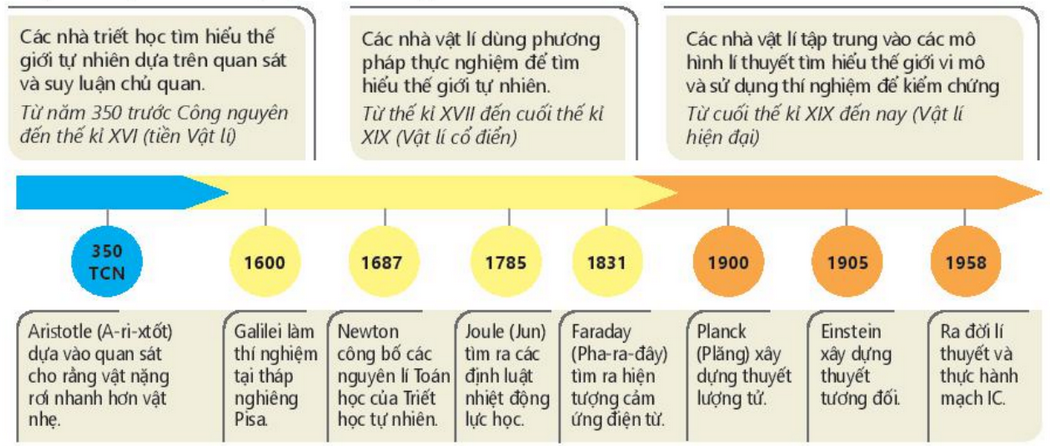
\includegraphics[width=0.95\textwidth]{../figs/G10-1-1}
\end{center}
\subsection{Phương pháp nghiên cứu của Vật lí}
Phương pháp nghiên cứu của Khoa học nói chung và Vật lí nói riêng được hình thành qua các thời kì phát triển của nền văn minh nhân loại, bao gồm hai phương pháp chính:
\begin{itemize}
	\item \textbf{\textit{Phương pháp thực nghiệm:}} dùng thí nghiệm để phát hiện kết quả mới giúp kiểm chứng, hoàn thiện, bổ sung hay bác bỏ giả thuyết nào đó. Kết quả mới này cần được giải thích bằng lí thuyết đã biết hoặc lí thuyết mới.
	\item \textbf{\textit{Phương pháp lí thuyết:}} sử dụng ngôn ngữ toán học và suy luận lí thuyết để phát hiện một kết quả mới. Kết quả mới này cần được kiểm chứng bằng thực nghiệm.
\end{itemize}
Hai phương pháp hỗ trợ cho nhau, trong đó phương pháp thực nghiệm có tính quyết định.\\
\textbf{Quy trình tìm hiểu thế giới tự nhiên dưới góc độ Vật lí}
\begin{center}
	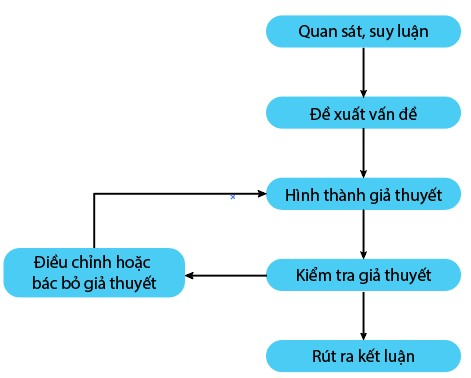
\includegraphics[width=0.6\linewidth]{../figs/VN10-2023-PH-TP002-1}
\end{center}
\subsection{Vai trò của vật lí đối với khoa học, kĩ thuật và công nghệ}
Vật Lý có quan hệ với mọi ngành khoa học và thường được coi là cơ sở của khoa học tự nhiên.

Ảnh hưởng của Vật Lý đến đời sống và kỹ thuật là vô cùng to lớn.
\subsubsection{Thông tin liên lạc}
Ngày nay, khoảng cách địa lí không còn là vấn đề quá lớn của con người trong thông tin liên lạc, sự bùng nổ của mạng lưới internet kết hợp sự phát triển vượt bậc của điện thoại thông minh (smartphone) giúp con người có thể chia sẻ thông tin liên lạc (hình ảnh, giọng nói, tin tức...) một cách dễ dàng. Thế giới ngày này là một thế giới “phẳng”.
\subsubsection{Y tế}
Hầu hết các phương pháp chuẩn đoán và chữa bệnh trong y học đều có cơ sở từ những kiến thức Vật Lý như: chụp X – quang, chụp cộng hưởng từ (MRI), siêu âm, nội soi, xạ trị, \dots
\subsubsection{Công nghiệp}
Cuộc cách mạng công nghiệp lần thứ tư được coi là bắt đầu thế kỉ XXI. Các nền sản xuất thủ công nhỏ lẻ được thay thế bởi những dây chuyền sản xuất tự động hóa, sử dụng trí tuệ nhân tạo, công nghệ vật liệu (nano), điện toán đám mây.
\subsubsection{Nông nghiệp}
Việc ứng dụng những thành tựu của Vật Lý vào nông nghiệp đã giúp cho người nông dân tiếp cận với nhiều phương pháp mới, ít tốn lao động, cho năng suất cao. 
\subsubsection{Nghiên cứu khoa học}
Vật lý góp phần to lớn trong việc cải tiến các thiết bị nghiên cứu khoa học ở nhiều ngành khác nhau như: kính hiển vi điện tử, nhiễu xạ tia X, máy quang phổ, \dots

\subsection{Một số quy định về an toàn trong phòng thực hành vật lí}
\subsubsection{Quy tắc an toàn trong sử dụng các thiết bị điện}
Cần quan sát kĩ các kí hiệu và nhãn thông số trên thiết bị để sử dụng đúng chức năng, đúng yêu cầu kĩ thuật.

Một số kí hiệu trên các thiết bị thí nghiệm:
\begin{center}
	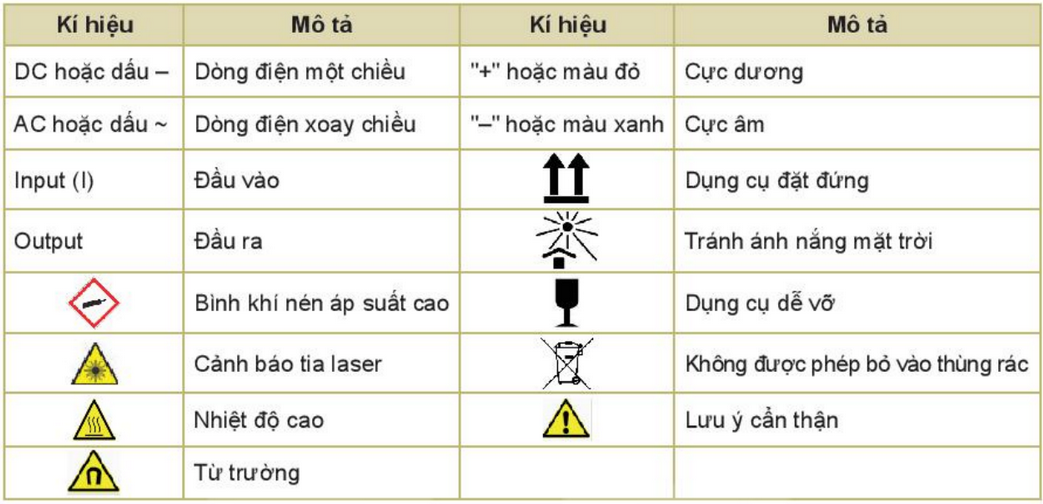
\includegraphics[scale=0.7]{../figs/G10-2-1}
\end{center}
\subsubsection{Quy tắc an toàn sử dụng các thiết bị nhiệt và thủy tinh}
Các thiết bị đun nóng có thể gây cháy hoặc nứt, vỡ các dụng cụ bằng thuỷ tinh.
\subsubsection{Quy tắc an toàn sử dụng các thiết bị quang học}
Các thiết bị quang học rất dễ bị mốc, xước, nứt, vỡ và dính bụi bẩn, làm ảnh hưởng đến đường truyền tia sáng và sai lệch kết quả thí nghiệm.
\section{Mục tiêu bài học - Ví dụ minh họa}
\begin{dang}{Nêu được đối tượng nghiên cứu của\\ vật lí học và mục tiêu của môn Vật lí}
	\viduii{1}{Hãy kể tên các lĩnh vực vật lí mà em đã được học ở cấp Trung học cơ sở.
	}
	{\hide{
		Ở cấp Trung học cơ sở, vật lí nghiên cứu các vấn đề cơ bản nhất của vật lí học, có thể kể đến như:
		\begin{itemize}
			%		\item Đo lường và các dụng cụ đo lường;
			\item Cơ học: Các chuyển động cơ học đơn giản, chuyển động dưới tác dụng của lực, năng lượng cơ học (cơ năng);
			\item Nhiệt học: Các đại lượng đặc trưng trong nhiệt học;
			\item Âm học: Các hiện tượng liên quan đến âm thanh;
			\item Điện học: Các mạch điện chứa điện trở, định luật cơ bản trong điện học;
			\item Quang học: Các dụng cụ quang học thường gặp, các định luật quang hình học.
		\end{itemize}
	}}


	\viduii{1}{Học tốt môn vật lí sẽ giúp ích gì cho em?
	}
	{\hide{
		Em hãy trao đổi với giáo viên và bày tỏ suy nghĩ của mình.
	}}
\end{dang}

\begin{dang}{Phân tích được một số ảnh hưởng của vật lí đối với cuộc sống, đối với sự phát triển của khoa học, công nghệ và kĩ thuật}
	\viduii{1}{Lấy ví dụ chứng tỏ tri thức vật lí giúp tránh được nguy cơ tổn hại về sức khỏe.
	}
	{\hide{
		Các em có thể lấy ví dụ vào các lĩnh vực nằm trong hiểu biết của mình:
		\begin{itemize}
			\item Kỹ thuật: chế tạo các công cụ, máy móc giúp tiết kiệm sức lao động;
			\item Công nghệ: chế tạo robot để thực hiện những công việc nguy hiểm;
			\item Y sinh: phẫu thuật bằng laser, siêu âm, chụp X-quang, xạ trị, $\ldots$; 
			\item Y học dự phòng: thay đổi thói quen sinh hoạt và làm việc khoa học dựa trên hoạt động của cơ, xương khớp; \dots
			\item Vật lí trị liệu: kích hoạt huyệt đạo trên cơ thể bằng dòng điện (châm cứu), sử dụng đèn hồng ngoại trong trị liệu, $\ldots$.
		\end{itemize}
	}}

	\viduii{1}{Lấy ví dụ và phân tích ảnh hưởng của vật lí đối với sự phát triển của khoa học kĩ thuật và công nghệ
	}
	{\hide{
		Các em có thể lấy ví dụ vào các lĩnh vực nằm trong hiểu biết của mình:
		\begin{itemize}
			\item Công nghiệp: tự động hoá trong hoạt động sản xuất nhờ ứng dụng điện - điện tử; sản xuất máy móc phục vụ công nghiệp dựa vào các kiến thức vật lí; \dots
			\item Nông nghiệp: cơ giới hoá trong sản xuất nông nghiệp. 
			\item Dịch vụ: sản xuất các phương tiện giao thông; truyền tin bằng sóng vô tuyến, wifi; $\ldots$.
		\end{itemize}
	}}
\end{dang}

\begin{dang}{Nêu được ví dụ về các phương pháp nghiên cứu vật lí}
	\viduii{2}
	{Vào đầu thế kỉ XX, J.J.Thomson đã đề xuất mô hình cấu tạo nguyên tử gồm các electron phân bố đều trong một khối điện dương kết cấu tựa như khối mây. Để kiểm chứng giả thuyết này, E. Rutherford đã sử dụng tia alpha gồm các hạt mang điện dương bắn vào các nguyên tử kim loại vàng Hình \ref{fig:2.2}. Kết quả của thí nghiệm đã bác bỏ giả thuyết của J. J. Thomson, đồng thời đã giúp khám phá ra hạt nhân nguyên tử. E. Rutherford đã vận dụng phương pháp nghiên cứu nào để nghiên cứu vấn đề này? Giải thích.
	\begin{center}
		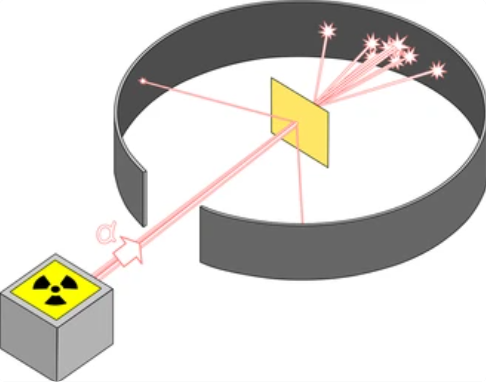
\includegraphics[width=0.3\linewidth]{../figs/VN10-2023-PH-TP002-2}
		\captionof{figure}{Thí nghiệm Rutherford.}
		\label{fig:2.2}
\end{center}  }
	{\hide{
		Rutherford đã sử dụng phương pháp thực nghiệm trong nghiên cứu vật lí vì ông đã thực hiện thí nghiệm dùng tia alpha gồm các hạt mang điện dương bắn vào các nguyên tử vàng để phát hiện ra kết quả mới chính là hạt nhân nguyên tử.
	}}
\end{dang}
\begin{dang}{Mô tả được các bước \\trong tiến trình tìm hiểu thế giới tự nhiên}
	\viduii{1}
	{Sắp xếp các bước tiến hành quá trình tìm hiểu thế giới tự nhiên dưới góc độ vật lí:\\
	\begin{enumerate}[label= (\arabic*)]
		\item Phân tích số liệu.
		\item Quan sát, xác định đối tượng cần nghiên cứu.
		\item Thiết kế, xây dựng mô hình kiểm chứng giả thuyết.
		\item Đề xuất giả thuyết nghiên cứu.
		\item Rút ra kết luận.
\end{enumerate} }
	{\hide{
	Tiến trình tìm hiểu thế giới tự nhiên dưới góc độ Vật lí là (2) - (4) - (3) - (1) - (5).
	}}
\end{dang}


\begin{dang}{Vận dụng được các quy tắc an toàn \\trong phòng thực hành vật lí}
	\viduii{2}{Hãy nêu quy tắc an toàn trong việc sử dụng các thiết bị sau:
		\begin{enumerate}
			\item Phích cắm điện;
			\item Dây điện;
			\item Nguồn tia LASER;
		\end{enumerate}
	}
	{\hide{
		\begin{enumerate}
			\item Phích cắm điện: Không chạm tay vào vị trí tiếp xúc giữa phích cắm và ổ điện, không cắm điện khi tay ướt.
			\item Dây điện: Không sử dụng dây điện cũ, không đấu nối dây điện thiếu an toàn.
			\item Nguồn tia LASER: Không đặt mắt trực tiếp trên đường truyền của tia LASER, không chiếu tia LASER vào người khác;
		\end{enumerate}
	}}

	\viduii{2}{Hãy cho biết các dụng cụ đo sau có chức năng gì và cách nối chúng vào mạch điện:
		\begin{enumerate}
			\item Ampe kế;
			\item Vôn kế;
			\item Đồng hồ đo điện đa năng.
		\end{enumerate}
	}
	{\hide{
		\begin{enumerate}
			\item Ampe kế: Dùng để đo cường độ dòng điện, nối tiếp với đoạn mạch cần đo;
			\item Vôn kế: Dùng để đo hiệu điện thế, mắc song song với đoạn mạch cần đo;
			\item Đồng hồ đo điện đa năng: Dùng để đo hiệu điện thế, cường độ dòng điện và điện trở, cần vặn núm xoay vào thang đo phù hợp trước khi tiến hành đo.
		\end{enumerate}
	}}
\end{dang}

%				\let\lesson\undefined
\newcommand{\lesson}{\phantomlesson{Bài 1+2.}}


\setcounter{section}{2}
\section{Bài tập trắc nghiệm}
\begin{enumerate}[label=\bfseries Câu \arabic*:,leftmargin=1.5cm]
	\item \mkstar{1}\\
	{Đối tượng nghiên cứu của Vật lí là gì?
		\begin{mcq}
			\item Các dạng vận động và tương tác của vật chất.
			\item Quy luật tương tác của các dạng năng lượng.
			\item Các dạng vận động của vật chất và năng lượng.
			\item Quy luật vận động, phát triển của sự vật - hiện tượng.
		\end{mcq}
}
\hideall{
\textbf{Đáp án: C.}
}

\item \mkstar{1}\\
{Lĩnh vực nghiên cứu nào sau đây là của Vật lí?
	\begin{mcq}
		\item Nghiên cứu về sự thay đổi của các chất khi kết hợp với nhau.
		\item Nghiên cứu sự phát triển của vi khuẩn.
		\item Nghiên cứu về sự hình thành và phát triển của các tầng lớp, giai cấp trong xã hội.
		\item Nghiên cứu về các dạng chuyển động và các dạng năng lượng khác nhau.
	\end{mcq}

}
\hideall{
\textbf{Đáp án: D.}
}

\item \mkstar{1}\\
{Cách sắp xếp nào sau đây trong 5 bước của phương pháp thực nghiệm là đúng?
	\begin{mcq}
		\item Xác định vấn đề cần nghiên cứu, dự đoán, quan sát, thí nghiệm, kết luận.
		\item Quan sát, xác định vấn đề cần nghiên cứu, thí nghiệm, dự đoán, kết luận.
		\item Xác định vấn đề cần nghiên cứu, quan sát, dự đoán, thí nghiệm, kết luận.
		\item Thí nghiệm, xác định vấn đề cần nghiên cứu, dự đoán, quan sát, kết luận.
	\end{mcq}
}
\hideall{
\textbf{Đáp án: C.}
}


\item \mkstar{2}\\
{Thành tựu nghiên cứu nào sau đây của Vật lí được coi là có vai trò quan trọng trong việc mở đầu cho cuộc cách mạng công nghệ lần thứ nhất?
	\begin{mcq}
		\item Nghiên cứu về lực vạn vật hấp dẫn.
		\item Nghiên cứu về nhiệt động lực học.
		\item Nghiên cứu về cảm ứng điện từ.
		\item Nghiên cứu về thuyết tương đối.
	\end{mcq}
}
\hideall{
\textbf{Đáp án: B.}
}


\item \mkstar{2}\\
{Trong các hoạt động dưới đây, những hoạt động nào tuân thủ nguyên tắc an toàn khi sử dụng điện?
	\begin{mcq}
		\item Bọc kĩ các dây dẫn điện bằng vật liệu cách điện.
		\item Kiểm tra mạch có điện bằng bút thử điện.
		\item Sửa chữa điện khi chưa ngắt nguồn điện.
		\item Chạm tay trực tiếp vào ổ điện, dây điện trần hoặc dây dẫn điện bị hở.
		\item Thường xuyên kiểm tra tình trạng hệ thống đường điện và các đồ dùng điện.
		\item Đến gần nhưng không tiếp xúc với các máy biến thế và lưới điện cao áp.
	\end{mcq}
}
\hideall{
\textbf{Đáp án: A, B, E.}
}

\item \mkstar{2}\\
{Trong các hoạt động dưới đây, những hoạt động nào tuân thủ nguyên tắc an toàn khi làm việc với các nguồn phóng xạ?
	\begin{mcq}
		\item Sử dụng phương tiện phòng hộ cá nhân như quần áo phòng hộ, mũ, găng tay, áo chì, \dots
		\item Ăn uống, trang điểm trong phòng làm việc có chứa chất phóng xạ.
		\item Tẩy xạ khi bị nhiễm bẩn phóng xạ theo quy định.
		\item Đổ rác thải phóng xạ tại các khu tập trung rác thải sinh hoạt.
		\item Kiểm tra sức khoẻ định kì.
	\end{mcq}
}
\hideall{
\textbf{Đáp án: A, C, E.}
}
\end{enumerate}
\section{Bài tập tự luận}
\setcounter{section}{0}

\begin{enumerate}[label=\bfseries Câu \arabic*:,leftmargin=1.5cm]
	\item \mkstar{2}
	
	
	{ 
		
		Quan sát thiết bị thí nghiệm về nhiệt học và trình bày đặc điểm của các dụng cụ thí nghiệm trên. Những điều cần chú ý để đảm bảo an toàn khi tiến hành thí nghiệm với các dụng cụ này là gì?
		\begin{center}
			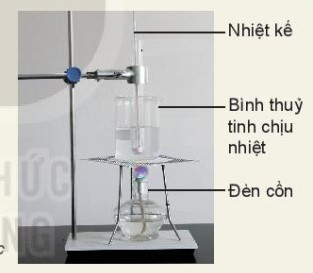
\includegraphics[scale=0.6]{../figs/VN10-2022-PH-TP003-3.jpg}
		\end{center}
	}
	
	\hideall
	{
		- Nhiệt kế: dùng để đo nhiệt độ của nước, hoạt động dựa trên cơ sở dãn nở vì nhiệt của các chất như: thủy ngân, rượu, ... được làm bằng thủy tinh dễ vỡ $\Rightarrow$ Khi tiến hành thí nghiệm cần cẩn thận, không để làm rơi, vỡ do thủy ngân trong nhiệt kế là một chất rất độc hại.
		
		- Bình thủy tinh chịu nhiệt: có thể chịu được nhiệt độ rất cao $\Rightarrow$ không dùng tay cầm trực tiếp vào bình.
		
		- Đèn cồn: dùng để đun sôi nước. Được thiết kế gồm:
		
		+ 1 bầu đựng cồn bằng thủy tinh
		
		+ 1 sợi bấc thường được dệt bằng sợi bông
		
		+ 1 chiếc chụp đèn bằng thủy tinh hoặc kim loại.
		
		$\Rightarrow$ \textbf{Lưu ý:}
		
		+ Không nên kéo sợi bấc quá dài
		
		+ Không trực tiếp thổi tắt ngọn lửa đèn cồn vì sẽ làm ngọn lửa cháy dữ dội hơn. Cách tốt nhất để tắt đèn là đậy nắp đèn cồn lại.
		
	}
	\item \mkstar{2}
	
	
	{
		Quan sát thiết bị thí nghiệm về quang học và trình bày đặc điểm của các dụng cụ thí nghiệm trên. Những điều cần chú ý để đảm bảo an toàn khi tiến hành thí nghiệm với các dụng cụ này là gì?
		
		\begin{center}
			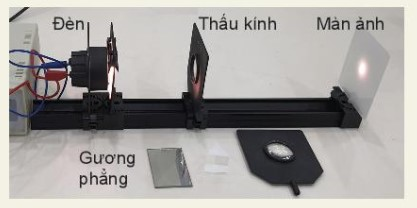
\includegraphics[scale=0.6]{../figs/VN10-2022-PH-TP003-4.jpg}
		\end{center}
	}
	
	\hideall
	{	
		- Đèn chiếu sáng: có kính tụ quang để tạo chùm tia song song, vỏ bằng nhôm hợp kim, có khe cài bản chắn sáng, có các vít điều chỉnh đèn. $\Rightarrow$ Tránh rơi, vỡ; để nơi khô thoáng.
		
		- Thấu kính: bằng thủy tinh, được lắp trong khung nhựa, gắn trên trụ nhôm $\Rightarrow$ Mỏng, dễ vỡ cần để trên cao, cất gọn gàng khi sử dụng xong.
		
		- Màn ảnh: có màu trắng mờ, gắn trên trụ nhôm $\Rightarrow$ Để nơi khô thoáng, tránh bụi bẩn.
		
		- Gương phẳng: bằng thủy tinh, dễ vỡ, sắc, nhọn $\Rightarrow$ Khi sử dụng cần cẩn thẩn, tránh va chạm mạnh hoặc rơi vỡ.
		
	}
	\item \mkstar{2}
	
	
	{
		Hãy quan sát một số hình ảnh về thao tác sử dụng các thiết bị thí nghiệm trong hình và dự đoán xem có những nguy cơ nào có thể gây nguy hiểm trong phòng thực hành vật lí.
		
		\begin{center}
			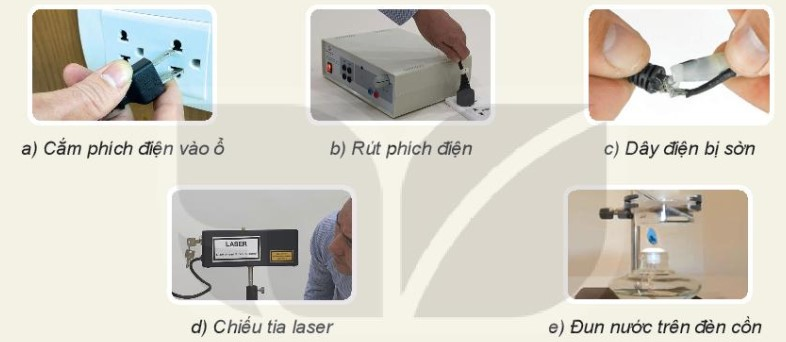
\includegraphics[scale=0.6]{../figs/VN10-2022-PH-TP003-5.jpg}
		\end{center}
	}
	
	\hideall
	{	
		\textbf{Nguy cơ có thể gây nguy hiểm}
		\begin{enumerate}[label=\alph*)]
			\item Cắm phích điện vào ổ: tay chạm vào phần kim loại dẫn điện ở phích điện $\Rightarrow$ bị giật.
			
			\item Rút phích điện: cầm vào phần dây điện, cách xa phích điện $\Rightarrow$ có thể làm dây điện bị đứt.
			
			\item Dây điện bị sờn: cầm tay trần vào dây điện mà không có đồ bảo hộ $\Rightarrow$ rất dễ bị giật điện.
			
			\item Chiếu tia laser: mắt nhìn trực tiếp vào tia laser gây nguy hiểm cho mắt.
			
			\item Đun nước trên đèn cồn: kẹp cốc thủy tinh quá gần với đèn cồn, bên dưới cốc không có lưới kim loại để phân tán nhiệt lượng (cốc sẽ dãn nở không đều) $\Rightarrow$ hư hỏng thiết bị thí nghiệm.
		\end{enumerate}
		
	}


	\item \mkstar{2}


{
	Hãy quan sát một số hình ảnh về thí nghiệm trong hình và dự đoán có những nguy cơ cháy nổ nào có thể xảy ra trong phòng thực hành.
	\begin{center}
		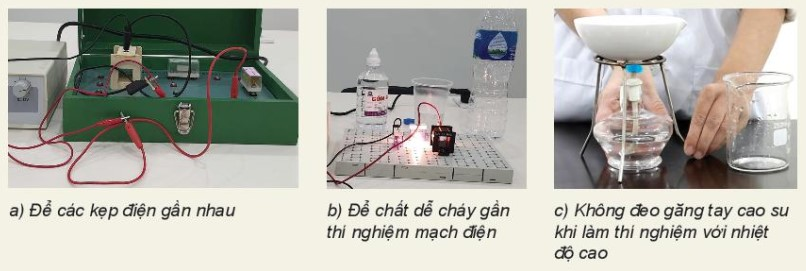
\includegraphics[scale=0.6]{../figs/VN10-2022-PH-TP003-7.jpg}
	\end{center}
}

\hideall
{	
	\begin{enumerate}[label=\alph*)]
		\item Để các kẹp điện gần nhau: có thể gây ra chập điện.
		\item Để chất dễ cháy gần mạch điện: nguy cơ cháy nổ.
		\item Không đeo găng tay cao su khi làm thí nghiệm với nhiệt độ cao, chạm tay trực tiếp vào đế kim loại khi đang đun: có thể bỏng.
	\end{enumerate}
}

	\item \mkstar{2}
	
	
	{
		Sử dụng động cơ điện có những ưu điểm vượt trội nào so với sử dụng máy hơi nước?
	}
	
	\hideall
	{	\begin{itemize}
			\item Ít tiêu tốn nhiên liệu vì hiệu suất chuyển hoá năng lượng cao.
			\item Hoạt động mạnh mẽ, tiết kiệm được thời gian vì động cơ điện có công suất lớn hơn nhiều so với động cơ hơi nước.
			\item Ít gây ô nhiễm môi trường do không phát thải khí thải thông qua quá trình đốt nhiên liệu.
		\end{itemize}
	}
	
	\item \mkstar{2}\\
	{Khí chiếu ánh sáng đến gương, ta quan sát thấy ánh sáng bị gương hắt trở lại môi trường cũ. Thực hiện những khảo sát chi tiết, ta có thể rút ra kết luận về nội dung định luật phản xạ ánh sáng như sau:
		\begin{itemize}
			\item Khi ánh sáng bị phản xạ, tia phản xạ sẽ nằm trong mặt phẳng chứa tia sáng tới và pháp tuyến của gương tại điểm tới.
			\item Góc phản xạ sẽ bằng góc tới.
		\end{itemize}
	Hãy xác định đối tượng cần nghiên cứu và phương pháp nghiên cứu trong khảo sát trên.
}
\hideall{
\begin{itemize}
	\item Đối tượng nghiên cứu: Sự truyền ánh sáng khi đến mặt gương.
	\item Phương pháp nghiên cứu: Phương pháp thực nghiệm.
\end{itemize}
}
	
	\item \mkstar{3}\\
	{Nhiều nhận định cho rằng: "Khoa học công nghệ ngày càng phát triển, bên cạnh việc chất lượng cuộc sống con người ngày càng được nâng cao thì con người cũng ngày càng đối diện với nhiều nguy hiểm". Em có ý kiến như thế nào về nhận định này? Bằng những hiểu biết Vật lí của mình, em hãy nếu các dẫn chứng cụ thể.
	
}
\hideall{
Học sinh đưa ra câu trả lời theo nhận định cá nhân:
\begin{itemize}
	\item Chất lượng cuộc sống con người ngày càng được nâng lên: nhiều thiết bị chăm sóc sức khoẻ, làm đẹp tại nhà; các thiết bị điện tự động hoặc điều khiển từ xa; vật dụng hiện đại trong nhà như bếp điện, nồi điện, máy hút bụi, \dots giúp cuộc sống con người tiện nghi hơn.
	\item Các nguy hiểm có thể có: rủi ro về điện như giật, cháy nổ, \dots; rủi ro phóng xạ từ các nhà máy điện hạt nhân; nguy cơ chiến tranh hạt nhân; \dots
\end{itemize}
}
	
	\item \mkstar{3}\\
	{Cho các biển báo như hình \ref{fig:2P-1}, hãy sắp xếp các biển này theo từng loại (biển báo cấm, biển báo nguy hiểm, biển thông báo) và cho biết ý nghĩa của từng biển báo.
		\begin{center}
			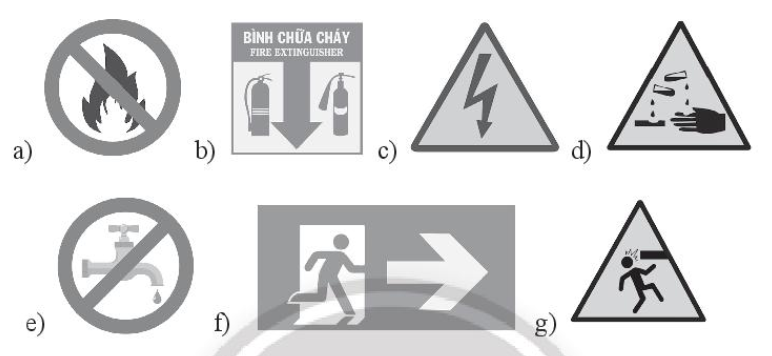
\includegraphics[width=0.6\linewidth]{../figs/VN10-2022-PH-TP002-P-1}
			\captionof{figure}{Một số biển báo}
			\label{fig:2P-1}
		\end{center}

}
\hideall{
\begin{itemize}
	\item Biển báo cấm: a (biển báo cấm lửa), e (biển báo cấm sử dụng nước).
	\item Biển báo nguy hiểm: c (biển cảnh báo nguy hiểm có điện), d (biển cảnh báo hoá chất ăn mòn), g (biển cảnh báo va chạm đầu).
	\item Biển thông báo: b (biển thông báo vị trí bình chữa cháy), f (biển thông báo lỗi thoát hiểm).
\end{itemize}
}

\item \mkstar{4}\\
{Ở những nơi nhiệt độ thấp (dưới $\SI{0}{\degree C}$), người ta nhận thấy rằng khi vung một lượng nước nhất định ra không khí thì nước nóng sẽ nhanh đông đặc hơn so với nước lạnh (Hình \ref{fig:2P-3}). Em hãy xây dựng tiến trình tìm hiểu hiện tượng trên, mô tả cụ thể các bước cần thực hiện, sau đó thực hiện tiến trình vừa xây dựng tại nhà và lưu lại kết quả thực hiện.\\
	\textit{Lưu ý: Chỉ nên sử dụng nước có nhiệt độ dưới $\SI{40}{\degree C}$ để đảm bảo an toàn trong quá trình thực hiện.}
	\begin{center}
		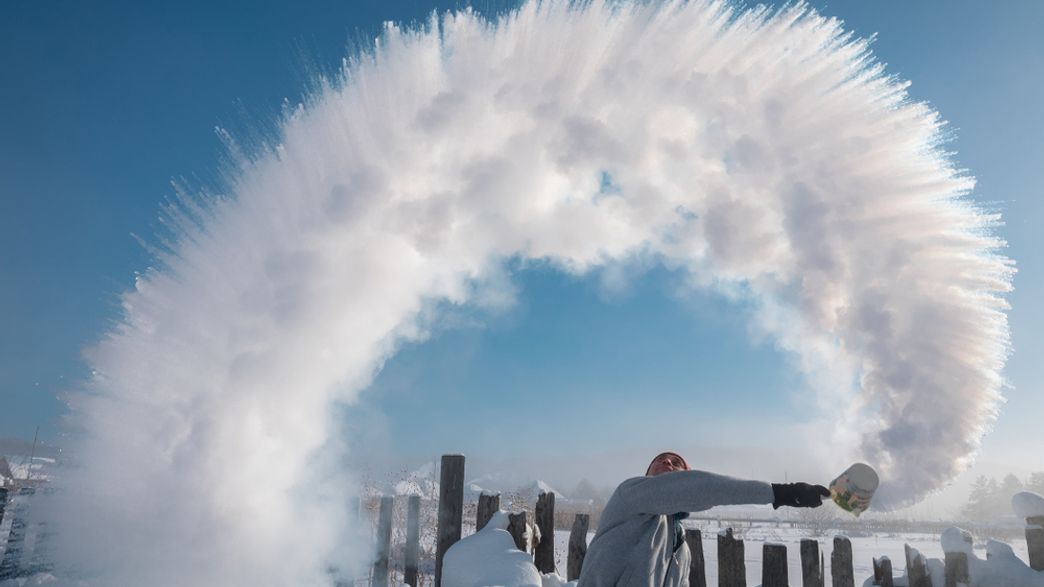
\includegraphics[width=0.3\linewidth]{../figs/VN10-2022-PH-TP002-P-3}
		\captionof{figure}{Nước nóng bị đông đặc ngay sau khi được vung ra ở nơi có nhiệt độ thấp.}
		\label{fig:2P-3}
	\end{center}
}
\hideall{
\textit{Tiến trình gợi ý:}\\
\begin{enumerate}[label=\arabic*.]
	\item Quan sát hiện tượng, các định đối tượng nghiên cứu: Nước nóng sẽ nhanh đông đặc hơn so với nước lạnh. Đối tượng nghiên cứu: Sự ảnh hưởng của nhiệt độ ban đầu đến thời gian đông đặc của nước.
	\item Giả thuyết đặt ra: Nước nóng đông đặc nhanh hơn nước lạnh.
	\item Lập phương án thực nghiệm: Khảo sát thời gian đông đặc của hai cốc nước có nhiệt độ khác nhau khi cho vào ngăn đông của tủ lạnh.
	\item Tiến hành thí nghiệm: Pha hai cốc nước (cùng thể tích) có nhiệt độ $\SI{5}{\degree C}$ và $\SI{35}{\degree C}$. Đặt hai cốc nước vào ngăn đông của tủ lạnh. Quan sát trạng thái đông đặc của hai cốc nước sau mỗi một giờ. Thu thập, xử lí và phân tích dữ liệu thực nghiệm.
	\item Rút ra kết luận.
\end{enumerate}
}
\end{enumerate}		
%			\stopMyChapterToc
%		\mychapter[Đơn vị và sai số trong vật lí]{Đơn vị và sai số trong vật lí}
%			\startMyChapterToc	
%				\let\lesson\undefined
\newcommand{\lesson}{\phantomlesson{Bài 3: Đơn vị và sai số trong vật lí}}
\chapter[Đơn vị và sai số trong vật lí]{Đơn vị và sai số trong vật lí}
\section{Lý thuyết}
\subsection{Đơn vị và thứ nguyên trong vật lí}
\subsubsection{Hệ đơn vị SI, đơn vị cơ bản và đơn vị dẫn xuất}
Tập hợp của đơn vị được gọi là hệ đơn vị. Trong khoa học có rất nhiều hệ đơn vị được sử dụng, trong đó thông dụng nhất là hệ đơn vị đo lường quốc tế SI (Système International d’unités) được xây dựng trên cơ sở của 7 đơn vị cơ bản.\\
Ngoài 7 đơn vị cơ bản, những đơn vị còn lại được gọi là đơn vị dẫn xuất. Mọi đơn vị dẫn xuất đều có thể phân tích thành các đơn vị cơ bản dựa vào mối liên hệ giữa các đại lượng tương ứng.\\
Khi số đo của đại lượng đang xem xét là một bội số hoặc ước số thập phân của mười, ta có thể sử dụng tiếp đầu ngữ như trong Bảng \ref{tab:1} ngay trước đơn vị để phần số đo được trình bày ngắn gọn.
\begin{table}[h]
	\centering
	\caption{Các đơn vị cơ bản trong hệ SI}
	\begin{tabular}{|c|c|c|c|}
		\hline
		\thead{STT} & \thead{Đơn vị} & \thead{Kí hiệu} & \thead{Đại lượng}\\
		\hline
		$1$ & \text{mét} & $\si{\meter}$ & \text{Chiều dài}\\
		\hline
		$2$ & \text{kilôgam} & $\si{\kilo\gram}$ & \text{Khối lượng}\\
		\hline
		$3$ & \text{giây} & $\si{\second}$ & \text{Thời gian}\\
		\hline
		$4$ & \text{kelvin} & $\si{\kelvin}$ & \text{Nhiệt độ}\\
		\hline
		$5$ & \text{ampe}& $\si{\ampere}$ & \text{Cường độ dòng điện}\\ 
		\hline
		$6$ & \text{mol} & $\si{\mole}$ & \text{Lượng chất}\\
		\hline
		$7$ & \text{candela} & $\si{\candela}$ & \text{Cường độ sáng}\\
		\hline
	\end{tabular}
\end{table}
\begin{table}[h]
	\centering
	\caption{Tên và kí hiệu tiếp đầu ngữ của bội số, ước số thập phân của đơn vị}
	\begin{tabular}{|c|c|c|c|c|c|}
		\hline
		\thead{Kí hiệu} & \thead{Tên đọc} & \thead{Hệ số} & \thead{Kí hiệu} & \thead{Tên đọc} & \thead{Hệ số}\\
		\hline
		Y & \text{yotta} & $10^{24}$ & \text{y} & \text{yokto} & $10^{-24}$\\
		\hline
		Z & \text{zetta} & $10^{21}$ & z & \text{zepto} & $10^{-21}$\\
		\hline
		E & \text{eta} & $10^{18}$ & \text{a} & \text{atto} & $10^{-18}$\\
		\hline
		P & \text{peta} & $10^{15}$ & f & \text{femto} & $10^{-15}$\\
		\hline
		T & \text{tera} & $10^{12}$ & p & \text{pico} & $10^{-12}$\\
		\hline
		G & \text{giga} & $10^{9}$ & n & \text{nano} & $10^{-9}$\\
		\hline
		M & \text{mega} & $10^{6}$ & \text{$\mu$} & \text{micro} & $10^{-6}$\\
		\hline
		k & \text{kilo} & $10^{3}$ & m & \text{mili} & $10^{-3}$\\
		\hline
		h & \text{hecto} & $10^{2}$ & c & \text{centi} & $10^{-2}$\\
		\hline
		da & \text{deka} & $10^{1}$ & d & \text{deci} & $10^{-1}$\\
		\hline
	\end{tabular}
	\label{tab:1}
\end{table}
\subsubsection{Thứ nguyên}
Thứ nguyên của một đại lượng là quy luật nêu lên sự phụ thuộc của đơn vị đo đại lượng đó vào các đơn vị cơ bản.
\begin{itemize}
	\item Thứ nguyên của một đại lượng $X$ được biễn diễn dưới dạng $[X]$. Thứ nguyên của một số đại lượng cơ bản thường sử dụng được thể hiện trong Bảng \ref{tab:2}.
	\item Một đại lượng vật lí có thể được biểu diễn bằng nhiều đơn vị khác nhau nhưng chỉ có một thứ nguyên duy nhất. Một số đại lượng vật lí có thể có cùng thứ nguyên.
\end{itemize}
\begin{center}
	\captionof{table}{Thứ nguyên của một số đại lượng cơ bản}
	\label{tab:2}
	\begin{tabular}{|c|c|}
		\hline
		\thead{Đại lượng cơ bản} & \thead{Thứ nguyên}\\
		\hline
		\text{[Chiều dài]} & $L$\\
		\hline
		\text{[Khối lượng]} & $M$\\
		\hline
		\text{[Thời gian]} & $T$\\
		\hline
		\text{[Cường độ dòng điện]} & $I$\\
		\hline
		\text{[Nhiệt độ]} & $K$\\
		\hline
	\end{tabular}
\end{center}
\luuy{Trong các biểu thức vật lí:
	\begin{itemize}
		\item Các số hạng trong phép cộng (hoặc trừ) phải có cùng thứ nguyên.
		\item Hai vế của một biểu thức vật lí có cùng thứ nguyên.
\end{itemize}}
\subsection{Sai số trong phép đo và cách hạn chế}
\subsubsection{Phép đo các đại lượng vật lí}
Phép đo một đại lượng vật lí là phép so sánh nó với đại lượng cùng loại được quy ước làm đơn vị.

Phép đo được phân loại thành 
\begin{itemize}
	\item \textbf{Phép đo trực tiếp} là phép xác định giá trị  một đại lượng bằng cách so sánh trực tiếp với dụng cụ đo (ví dụ như đo khối lượng bằng cân, đo nhiệt độ bằng nhiệt kế). 
	\item \textbf{Phép đo gián tiếp} là phép xác định giá trị một đại lượng thông qua một công thức liên hệ với các đại lượng được đo trực tiếp (ví dụ như đo khối lượng riêng thông qua việc xác định khối lượng và thể tích của khối vật chất).   
\end{itemize}
\subsubsection{Các loại sai số của phép đo}
\begin{center}
	\captionof{table}{Các loại sai số của phép đo}
	\begin{longtable}{|m{5em}|m{20em}|m{20em}|}
		\hline
		&\thead{Sai số hệ thống} & \thead{Sai số ngẫu nhiên}\\
		\hline
		\text{Khái niệm} & Sai số hệ thống là sai số có tính quy luật và được lặp lại ở tất cả các lần đo. Sai số hệ thống làm cho giá trị đo tăng hoặc giảm một lượng nhất định so với giá trị thực. & Sai số ngẫu nhiên là sai số xuất phát từ sai sót, phản xạ của người làm thí nghiệm hoặc từ những yếu tố ngẫu nhiên bên ngoài.\\
		\hline
		\text{Nguyên nhân} & Các dụng cụ đo các đại lượng vật lí luôn có sự sai lệch do đặc điểm và cấu tạo của dụng cụ gây ra. & Sai số này thường có nguyên nhân không rõ ràng và dẫn đến sự phân tán của các kết quả đo xung quanh một giá trị trung bình.\\
		\hline
		\text{Cách hạn chế} & Sai số hệ thống có thể được hạn chế bằng cách thường xuyên hiệu chỉnh dụng cụ đo, sử dụng thiết bị đo có độ chính xác cao. & Sai số ngẫu nhiên có thể được hạn chế bằng cách thực hiện phép đo nhiều lần và lấy giá trị trung bình để hạn chế sự phân tán của số liệu đo.\\
		\hline
	\end{longtable}
\end{center}
\luuy{Đối với một số dụng cụ đo, sai số dụng cụ thường được xác định bằng một nửa độ chia nhỏ nhất.}
\subsubsection{Cách biểu diễn sai số của phép đo}
Khi đo $n$ lần cùng một đại lượng $A$, ta thu được các giá trị khác nhau: $A_1,\, A_2,\,...,A_n$

Giá trị trung bình khi đo nhiều lần một đại lượng $A$:$$\bar{A}=\dfrac{A_1+A_2+...+A_{\text{n}}}{n},$$
là giá trị gần đúng nhất với giá trị thực của đại lượng $A$.  
\begin{itemize}
	\item Sai số tuyệt đối ứng với mỗi lần đo:
	$$\Delta A_1=|\bar{A}-A_1|;\quad\Delta A_2=|\bar{A}-A_2|;\quad\Delta A_3=|\bar{A}-A_3|;\dots; \Delta A_i=\left|\overline{A}-A_i\right|$$
	\item Sai số ngẫu nhiên là sai số tuyệt đối trung bình của $n$ lần đo:
	$$\overline{\Delta A}=\dfrac{\Delta A_1+\Delta A_2+...+\Delta A_{\textrm{n}} }{n}.$$
	\item Sai số dụng cụ $\Delta A_\text{dc}$ thường được lấy bằng nửa độ chia nhỏ nhất đối với những dụng cụ đơn giản như thước kẻ, cân bàn, bình chia độ, \dots Trong nhiều trường hợp, sai số dụng cụ thường được cung cấp chính xác bởi nhà sản xuất.
	\item Sai số tuyệt đối của phép đo cho biết phạm vi biến thiên của giá trị đo được và bằng tổng của sai số ngẫu nhiên và sai số dụng cụ:
	$$\Delta A= \overline{\Delta A}+ \Delta A_\text{dc}.$$
\end{itemize}
\subsubsection{Sai số tương đối (tỉ đối)}
Sai số tỉ đối $\delta A$ của phép đo là tỉ số giữa \bltext{sai số tuyệt đối} và \bltext{giá trị trung bình} của đại lượng cần đo, tính bằng phần trăm:
$$\delta A=\dfrac{\Delta A}{\overline A}\cdot 100\%.$$
Sai số tỉ đối càng \bltext{nhỏ} thì phép đo càng chính xác.

\subsubsection{Cách xác định sai số của phép đo gián tiếp}
Sai số của phép đo gián tiếp, được xác định theo các quy tắc:
\begin{itemize}
	\item Sai số tuyệt đối của một tổng hay hiệu thì bằng \bltext{tổng} các sai số tuyệt đối của các số hạng:\\
	Nếu $F=x\pm y\pm z \dots$ thì $\Delta F = \Delta x + \Delta y + \Delta z+\dots$.
	\item Sai số tỉ đối của một tích hay thương thì bằng \bltext{tổng} các sai số tỉ đối của các thừa số:\\ 
	Nếu $F= x^m\cdot\dfrac{y^n}{z^k}$ thì $\delta F=m\cdot\delta x+n\cdot\delta y +k\cdot\delta z$.
\end{itemize}
\textbf{Quy tắc xác định số chữ số có nghĩa (CSCN):}\\
Các chữ số có nghĩa bao gồm:
\begin{itemize}
	\item Các chữ số khác 0.
	\item Các chữ số 0 nằm giữa hai chữ số khác 0.
	\item Các chữ số 0 nằm bên phải của dấu	thập phân và một chữ số khác 0
\end{itemize}
\textit{Ví dụ:} \textbf{678} có ba chữ số có nghĩa, \textbf{6008} có bốn chữ số có nghĩa, 0,0\textbf{800} có ba chữ số có nghĩa.
\subsubsection{Cách viết kết quả đo}
$$A=\overline{A} \pm \Delta A,$$
trong đó:
\begin{itemize}
	\item $\overline A$ là giá trị trung bình,
	\item $\Delta A$ là sai số tuyệt đối. 
\end{itemize}
\section{Mục tiêu bài học - Ví dụ minh hoạ}
\begin{dang}{Tìm hiểu một số loại sai số đơn giản hay gặp khi đo các đại lượng vật lí và cách khắc phục chúng}
	\viduii{2}{
	Quan sát các hình sau và phân tích các nguyên nhân gây ra sai số của phép đo trong các trường hợp được nêu
	\begin{center}
		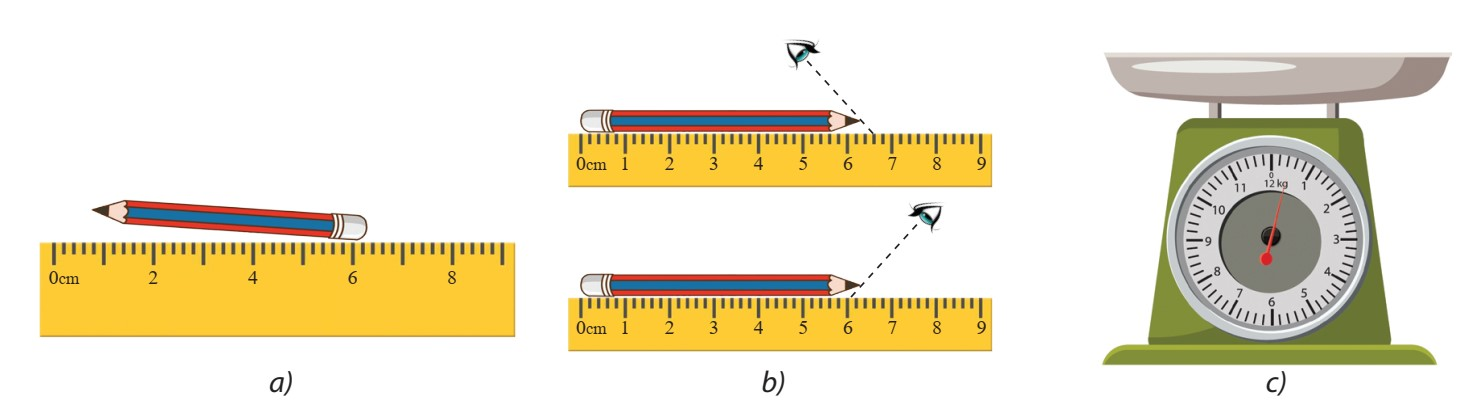
\includegraphics[width=0.7\linewidth]{../figs/VN10-2023-PH-TP003-1}
	\end{center}
}{\hide{
\begin{enumerate}[label=\alph*)]
	\item Đặt bút không dọc theo thước, đầu bút không trùng với vạch số 0.
	\item Đặt mắt sai cách, hướng nhìn không vuông góc.
	\item Kim cân chưa được hiệu chỉnh về số 0.
\end{enumerate}
}}
\end{dang}
\begin{dang}{Vận dụng mối liên hệ giữa đơn vị dẫn xuất với 7 đơn vị cơ bản của hệ SI}
	\viduii{3}
	{Để xác định quãng đường đi được $s$ của một chất điểm chuyển động thẳng đều, một bạn học sinh đã viết công thức như sau: $s=\alpha\cdot v\cdot t^2$ với $v$ và $t$ lần lượt là vận tốc và thời gian, $\alpha$ là hằng số không thứ nguyên. Dựa vào việc xác định thứ nguyên, em hãy cho biết công thức trên là đúng hay sai.
	}
{\hide{
	Thứ nguyên của các đại lượng $s$, $v$ và $t$ lần lượt là
	\begin{itemize}
		\item $\left[s\right]=L$
		\item $\left[v\right]=L\cdot T^{-1}$
		\item $\left[t\right]=T$
	\end{itemize}
Từ đó, ta thấy vế trái của công thức trên có thứ nguyên $L$ trong khi vế phải lại có thứ nguyên $L\cdot T$. Do 2 vế của công thức không cùng thứ nguyên nên bạn học sinh chưa đưa ra được công thức chính xác.\\
Dựa vào phân tích thứ nguyên, ta cần sửa lại công thức chính xác như sau:
$$s=\alpha \cdot v\cdot t$$
Trong hệ SI, $s$, $v$ và $t$ lần lượt có đơn vị là $\si{\meter}, \si{\meter\cdot\second^{-1}}, \si{\second}$.
}}
	
\end{dang}
\begin{dang}{Xác định được sai số tuyệt đối,\\ sai số tỉ đối và biểu diễn được kết quả đo}
	\viduii{3}
	{Cho bảng số liệu thể hiện kết quả đo đường kính của một viên bi thép bằng thước kẹp có sai số dụng cụ là $\SI{0.02}{\milli\meter}$. Tính sai số tuyệt đối, sai số tương đối của phép đo và biểu diễn kết quả đo có kèm theo sai số
		\begin{longtable}{|c|c|c|}
			\hline
			\thead{Lần đo} & \thead{$d \left(\si{\milli\meter}\right)$} & \thead{$\Delta d \left(\si{\milli\meter}\right)$}\\
			\hline
			1 & 6,32 & \dots\\
			\hline
			2 & 6,32 & \dots\\
			\hline
			3 & 6,32 & \dots\\
			\hline
			4 & 6,32 & \dots\\
			\hline
			5 & 6,34 & \dots\\
			\hline
			6 & 6,34 & \dots\\
			\hline
			7 & 6,32 & \dots\\
			\hline
			8 & 6,34 & \dots\\
			\hline
			9 & 6,32 & \dots\\
			\hline
			\textbf{Trung bình} & $\overline{d}=?$ & $\overline{\Delta d}=?$\\
			\hline
		\end{longtable}
	
}
{\hide{
Giá trị trung bình của đường kính viên bi:
$$\overline{d}=\dfrac{d_1+d_2+d_3+\dots+d_9}{9}\approx\SI{6.327}{\milli\meter}$$
Sai số tuyệt đối ứng với mỗi lần đo
$$\Delta d_i=\left|\overline{d}-d_i\right|$$
$$\Delta d_1=\Delta d_2=\Delta d_3=\Delta d_4=\Delta d_7=\Delta d_9=\left|\SI{6.327}{\milli\meter}-\SI{6.32}{\milli\meter}\right|=\SI{0.007}{\milli\meter}$$
$$\Delta d_5=\Delta d_6=\Delta d_8=\left|\SI{6.327}{\milli\meter}-\SI{6.34}{\milli\meter}\right|=\SI{0.013}{\milli\meter}$$
Sai số tuyệt đối trung bình của phép đo:
$$\overline{\Delta d}=\dfrac{\Delta d_1+\Delta d_2+\dots+\Delta d_9}{9}=\SI{0.009}{\milli\meter}$$
Sai số tuyệt đối của phép đo:
$$\Delta d = \overline{\Delta d}+\Delta d_\text{dc}=\SI{0.009}{\milli\meter}+\SI{0.02}{\milli\meter}=\SI{0.029}{\milli\meter}$$
Sai số tương đối của phép đo:
$$\delta d =\dfrac{\Delta d}{\overline{d}}\cdot\SI{100}{\percent}\approx\SI{0.46}{\percent}$$
Kết quả phép đo:
$$d=\overline{d}\pm\Delta d=6,273\pm\SI{0.029}{\milli\meter}.$$
}}
\end{dang}
\begin{dang}{Xác định sai số gián tiếp}
	\viduii{3}{Trong bài thực hành đo gia tốc trọng trường của Trái Đất tại phòng thí nghiệm, một học sinh đo được chiều dài của con lắc đơn $\ell= \xsi{800\pm 1}{\milli\meter}$ thì chu kì dao động là $T = \xsi{1,78\pm 0,02}{\second}$. Lấy $\pi=\SI{3.14}{}$. Biết chu kỳ của con lắc đơn tính theo công thức $T=2\pi \sqrt{\dfrac{\ell}{g}}$. Gia tốc trọng trường $g$ của Trái Đất tại phòng thí nghiệm đó là bao nhiêu?
	}
	{\hide{
		Từ công thức: $$T=2\pi \sqrt{\dfrac{\ell}{g}} \Rightarrow g=\dfrac{4\pi^2\ell}{T^2}.$$ 	
		
		Giá trị trung bình của gia tốc trọng trường: 	
		$$\overline{g}=\dfrac{4\pi^2\ell}{T^2}=\dfrac{4\pi^2\cdot \SI{3.14}{}^2\cdot \SI{0.8}{\meter}}{\left( \SI{1.78}{\second}\right)^2}=\SI{9.96}{\meter\per\second^2}.$$
		
		Sai số tuyệt đối của gia tốc trọng trường:
		\begin{align*}
			\dfrac{\Delta g}{\overline g}&= \dfrac{\Delta \ell}{\overline \ell}+ 2\dfrac{\Delta T}{\overline T}\\
			&=\dfrac{\SI{1}{\milli\meter}}{\SI{800}{\milli\meter}}+2\times\dfrac{\SI{0.02}{\second}}{\SI{1.78}{\second}}\\
			&=\SI{0.024}{}\\
			\Rightarrow\quad \Delta g&= \SI{0.024}{}\cdot \overline g\\
			&= \SI{0.24}{\meter\per\second^2}.
		\end{align*}
		
		
		
		Vậy gia tốc trọng trường của Trái Đất tại phòng thí nghiệm đó là
		$$g={\overline g } \pm \Delta g =9,96\pm\SI{0.24}{\meter\per\second^2}.$$
	}}


	\viduii{3}{Một học sinh dùng cân và đồng hồ đếm giây để đo độ cứng $k$ của lò xo. Dùng cân để cân vật nặng thu được kết quả khối lượng $m = 100 \,\text{g}$ với sai số tỉ đối là $2\%$. Gắn vật vào lò xo và kích thích cho con lắc dao động rồi dùng đồng hồ đếm giây đo thời gian của một dao động cho kết quả $T = 2\,\text{s}$ với sai số tỉ đối là $1\%$. Biết chu kỳ của con lắc lò xo tính theo công thức $T=2\pi \sqrt{m/k}$. Sai số tỉ đối của phép đo độ cứng của lò xo là bao nhiêu?
	}
	{\hide{
		Từ công thức: $$T=2\pi \sqrt{\dfrac{m}{k}} \Rightarrow k=\dfrac{4\pi^2m}{T^2}.$$	
		
		Sai số tỉ đối của độ cứng lò xo: 	
		$$\dfrac{\Delta k}{\overline k}= \dfrac{\Delta m}{\overline m}+ 2\dfrac{\Delta T}{\overline T}= 2\%+2\cdot 1\%= 4\%.$$
		
		Vậy sai số tỉ đối của phép đo độ cứng của lò xo là $4\%.$
	}}
\end{dang}

%				\let\lesson\undefined
\newcommand{\lesson}{\phantomlesson{Bài 3.}}


\setcounter{section}{2}
\section{Bài tập trắc nghiệm}
\begin{enumerate}[label=\bfseries Câu \arabic*:,leftmargin=1.5cm]
\item \mkstar{1}\\
{Chọn đáp án có từ /cụm từ thích hợp để hoàn thành bảng sau:
	\begin{center}
		\begin{tabular}{|c|c|c|}
			\hline
			\thead{Đơn vị} & \thead{Kí hiệu} & \thead{Đại lượng }\\
			\hline
			kelvin & (1) & (2)\\
			\hline
			ampe & $\si{\ampere}$ & (3)\\
			\hline
			candela & $\si{\candela}$ & (4)\\
			\hline
		\end{tabular}
	\end{center}
\begin{mcq}
	\item (1) $\si{\kelvin}$; (2) Khối lượng; (3) Cường độ dòng điện; (4) Lượng chất.
	\item (1) $\si{\kelvin}$; (2) Nhiệt độ; (3) Cường độ dòng điện; (4) Cường độ ánh sáng.
	\item (1) $\si{\kelvin}$; (2) Nhiệt độ; (3) Cường độ dòng điện; (4) Lượng chất.
	\item (1) $\si{\kelvin}$; (2) Khối lượng; (3) Cường độ dòng điện; (4) Cường độ ánh sáng.
\end{mcq}
}
\hideall{
\textbf{Đáp án: B.}
}

\item \mkstar{1}\\
{Đơn vị nào sau đây không thuộc thứ nguyên $L$ [Chiều dài]?
	\begin{mcq}(4)
		\item Dặm.
		\item Hải lí.
		\item Năm ánh sáng.
		\item Năm.
	\end{mcq}
}
\hideall{
\textbf{Đáp án: D.}
}


\item \mkstar{1}\\
{Chọn đáp án có từ/cụm từ thích hợp để hoàn thành các câu sau:
	\begin{itemize}
		\item[-] Các số hạng trong phép cộng (hoặc trừ) phải có cùng (1) \dots và nên chuyển về cùng (2) \dots.
		\item[-] (3) \dots của một biểu thức vật lí phải có cùng thứ nguyên.
	\end{itemize}
\begin{mcq}
	\item (1) đơn vị; (2) thứ nguyên; (3)  Đại lượng.
	\item (1) thứ nguyên; (2) đại lượng; (3) Hai vế.
	\item (1) đơn vị; (2) đại lượng; (3) Hai vế.
	\item (1) thứ nguyên; (2) đơn vị; (3) Hai vế.
\end{mcq}
}
\hideall{
\textbf{Đáp án: D.}
}

\item \mkstar{2}\\
Trong hệ đơn vị SI, tốc độ có đơn vị là
\begin{mcq}(4)
	\item $\si{\kilo\meter/\hour}$.
	\item $\si{\meter/\second}$.
	\item $\si{\text{dặm}/\hour}$.
	\item $\si{ft/\second}$.
\end{mcq} 
\hideall{
	\textbf{Đáp án B.}
}


\item \mkstar{2}\\
{Trong các phép đo dưới đây, đâu là phép đo trực tiếp?
	\begin{enumerate}[label=(\arabic*)]
		\item Dùng thước đo chiều cao.
		\item Dùng cân đo cân nặng.
		\item Dùng cân và ca đong đo khối lượng riêng của nước.
		\item Dùng đồng hồ và cột cây số đo tốc độ của người lái xe.
	\end{enumerate}
\begin{mcq}(4)
	\item (1), (2).
	\item (1), (2), (4).
	\item (2), (3), (4).
	\item (2), (4).
\end{mcq}
}
\hideall{
\textbf{Đáp án: A.}
}

\item \mkstar{2}\\
{Đáp án nào sau đây có 1 đơn vị cơ bản và 1 đơn vị dẫn xuất?
	\begin{mcq}(2)
		\item mét, kilogram.
		\item newton, mol.
		\item pascal, joule.
		\item candela, kelvin.
	\end{mcq}
}
\hideall{
\textbf{Đáp án: B.}
}

\item \mkstar{2}\\
{Giá trị nào sau dây có 2 chữ số có nghĩa (CSCN)?
	\begin{mcq}(4)
		\item $\SI{201}{\meter}$.
		\item $\SI{0.02}{\meter}$.
		\item $\SI{20}{\meter}$.
		\item $\SI{210}{\meter}$.
	\end{mcq}

}
\hideall{
\textbf{Đáp án: D.}
}

\item \mkstar{3}\\
{Một bánh xe có bán kính $R=\xsi{10\pm0,5}{\centi\meter}$. Sai số tương đối của chu vi bánh xe là
	\begin{mcq}(4)
		\item $\SI{0.05}{\percent}$.
		\item $\SI{5}{\percent}$.
		\item $\SI{10}{\percent}$.
		\item $\SI{25}{\percent}$.
	\end{mcq}
}
\hideall{
\textbf{Đáp án: B.}\\
$$\delta R=\dfrac{\Delta R}{\overrightarrow{R}}\cdot\SI{100}{\percent}=\SI{5}{\percent}.$$
}

\item \mkstar{3}\\
Thứ nguyên của vận tốc là
\begin{mcq}(4)
	\item $LT$.
	\item $L^{-1}T$.
	\item $L^{-1}T^{-1}$.
	\item $LT^{-1}$.
\end{mcq}
\hideall{
\textbf{Đáp án D.}\\
\begin{eqnarray*}
	v&=&\dfrac{s}{t}\\
	\Rightarrow \left[v\right]&=&\dfrac{\left[s\right]}{\left[t\right]}=LT^{-1}.
\end{eqnarray*}
}

\item \mkstar{3}\\
Thứ nguyên của trọng lượng riêng là
\begin{mcq}(4)
	\item $MLT^{-1}$.
	\item $MLT^{-2}$.
	\item $ML^{-2}T^{-1}$.
	\item $ML^{-2}T^{-2}$.
\end{mcq}
\hideall{
\textbf{Đáp án D.}\\
\begin{eqnarray*}
	d&=&\dfrac{P}{V}\\
	\Rightarrow \left[d\right]&=&\dfrac{\left[P\right]}{\left[V\right]}\\
	\Leftrightarrow \left[d\right]&=&\dfrac{MLT^{-2}}{L^3}=ML^{-2}T^{-2}.
\end{eqnarray*}
}
\end{enumerate}
\section{Bài tập tự luận}
\begin{enumerate}[label=\bfseries Bài \arabic*:,leftmargin=1.5cm]
	\item 
	\mkstar{2}\\
	Một học sinh làm thí nghiệm đo chiều dài của bàn học bằng thước. Sau 6 lần đo, bạn học sinh tính được:
	\begin{itemize}
		\item Giá trị trung bình chiều dài bàn là $\overline{\ell}=\SI{1202}{\milli\meter}$.
		\item Sai số trung bình là $\overline{\Delta\ell}=\SI{2}{\milli\meter}$.
	\end{itemize}
Biết sai số dụng cụ đo là $\Delta \ell_\text{dc}=\SI{1}{\milli\meter}$.\\
Bạn hãy trình bày kết quả phép đo của học sinh trên.
\hideall{
Sai số tuyệt đối của phép đo:
$$\Delta \ell=\overline{\Delta \ell}+\Delta\ell_\text{dc}=\SI{3}{\milli\meter}.$$
Kết quả phép đo:
$$\ell=\overline{\ell}+\Delta\ell=\xsi{1202\pm3}{\milli\meter}.$$
}
	\item \mkstar{2}
	
	
	{
		Em hãy lập phương án đo tốc độ chuyển động của ô tô đồ chơi, chỉ dùng thước và đồng hồ bấm giây để trả lời các câu hỏi sau:
		\begin{enumerate}[label=\alph*)]
			\item Để đo tốc độ chuyển động của chiếc xe, cần đo những đại lượng nào?
			\item Xác định tốc độ chuyển động của xe theo công thức nào?
			\item Phép đo nào là phép đo trực tiếp? Tại sao?
			\item Phép đo nào là phép đo gián tiếp? Tại sao?
		\end{enumerate}
		
	}
	
	\hideall
	{	
		\begin{enumerate}[label=\alph*)]
			\item Để đo tốc độ chuyển động của chiếc xe, cần đo những đại lượng: đo quãng đường xe di chuyển được và thời gian xe di chuyển.
			\item Xác định tốc độ chuyển động của xe theo công thức:
			
			$$v = \dfrac{s}{t}.$$
			
			\item Phép đo quãng đường và thời gian là phép đo trực tiếp. Vì ta thực hiện động tác trực tiếp lên các dụng cụ thí nghiệm.
			\item Phép đo xác đinh vận tốc là phép đo gián tiếp. Vì phép đo này có được cần phải thông qua hai phép đo kia.
		\end{enumerate}
	}

\item \mkstar{2}\\
{Hình \ref{fig:3P-1} thể hiện nhiệt kế đo nhiệt độ $t_1$ $\left(\si{\degree C}\right)$ và $t_2$ $\left(\si{\degree C}\right)$ của một dung dịch trước và sau khi đun. Hãy xác định và ghi kết quả độ tăng nhiệt độ $t$ của dung dịch này.
	\begin{center}
		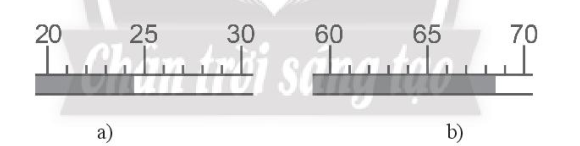
\includegraphics[width=0.4\linewidth]{../figs/VN10-2022-PH-TP003-P-1}
		\captionof{figure}{Nhiệt kế: \textit{a) trước; b) sau khi đun dung dịch}}
		\label{fig:3P-1}
	\end{center}
}
\hideall{
Lấy sai số dụng cụ $\Delta t_\text{dc}=\dfrac{\text{ĐCNN}}{2}=\SI{0.5}{\degree C}$.\\
Nhiệt độ ban đầu:
$$t_1=\xsi{24\pm0,5}{\degree C}$$
Nhiệt độ lúc sau:
$$t_2=\xsi{68\pm 0,5}{\degree C}$$
Đồ tăng nhiệt độ của dung dịch này:
$$t=t_2-t_1=\xsi{44,0\pm1,0}{\degree C}.$$
}

\item \mkstar{2}\\
{Hãy xác định số CSCN của các số sau đây: $123,45$; $1,990$; $3,110\cdot 10^{-9}$; $1907,21$; $0,002099$; $12768000$. 

}
\hideall{
$123,45$ - 5 CSCN; $1,990$ - 4 CSCN; $3,110\cdot10^{-9}$ - 4 CSCN; $1907,21$ - 6 CSCN; $0,002099$ - 4 CSCN; $12768000$ - 5 CSCN.
}
	
	\item \mkstar{2}\\
	{Một viên bị hình cầu có bán kính $r$ đang chuyển động với tốc độ $v$ trong dầu. Viên bị chịu tác dụng của lực cản có độ lớn được cho bởi biểu thức $F=c\cdot r\cdot v$, trong đó $c$ là một hằng số. Xác định đơn vị của $c$ theo đơn vị của lực, chiều dài và thời gian trong hệ SI.
}
\hideall{
	Từ công thức trên đề bài $\Rightarrow c=\dfrac{F}{r\cdot v}$\\
Đơn vị của $c$ là: $\si{\newton\cdot\meter^{-2}\cdot\second}$.
}
	
	\item \mkstar{2}\\
	{Một vật có khối lượng $m$ và thể tích $V$, có khối lượng riêng $\rho$ được xác định bằng công thức $\rho =\dfrac{m}{V}$. Biết sai số tương đối của phép đo $m$ và $V$ lần lượt là $\SI{12}{\percent}$ và $\SI{5}{\percent}$. Hãy xác định sai số tương đối của phép đo $\rho$.
	
}
\hideall{
$$\delta \rho=\delta m+\delta V=\SI{12}{\percent}+\SI{5}{\percent}=\SI{17}{\percent}.$$
}
	
	\item \mkstar{2}\\
	{Một học sinh muốn xác định gia tốc rơi tự do $g$ bằng cách thả một quả bóng từ độ cao $h$ và dùng đồng hồ để bấm thời gian rơi $t$ của quả bóng. Sau đó, thông qua quá trình tìm hiểu, bạn sử dụng công thức $h=\dfrac{1}{2}g\cdot t^2$ để xác định $g$. Hãy nêu ít nhất 2 giải pháp giúp bạn học sinh đó giảm sai số trong quá trình thực nghiệm để thu được kết quả chính xác nhất.
	
}
\hideall{
Một số giải pháp phù hợp: hạn chế sự tác động của lực cản không khí, thả rơi quả bóng ở nhiều độ cao khác nhau, sử dụng đồng hồ có độ nhạy cao, thao tác bấm đồng hồ dứt khoát.
}

\item \mkstar{2}


{
	\begin{center}
		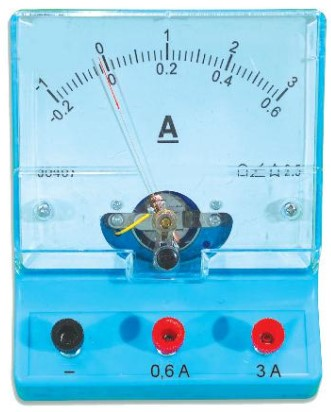
\includegraphics[scale=0.6]{../figs/VN10-2022-PH-TP003-6.jpg}
	\end{center}
	\begin{enumerate}[label=\alph*)]
		\item Giới hạn đo của ampe kế là bao nhiêu?
		\item Nếu sử dụng ampe kế để đo dòng điện vượt quá giới hạn đo thì có thể gây ra nguy cơ gì?
	\end{enumerate}
}

\hideall
{	
	\begin{enumerate}[label=\alph*)]
		\item Giới hạn đo của ampe kế ở hình là $\SI{3}{A}$.
		\item Nếu sử dụng ampe kế để đo dòng điện vượt quá giới hạn đo thì có thể làm cho ampe kế bị hư hỏng.
	\end{enumerate}
}



\item \mkstar{3}\\
{Hãy xác định số đo chiều dài của cây bút chì trong các trường hợp dưới đây:
	\begin{center}
		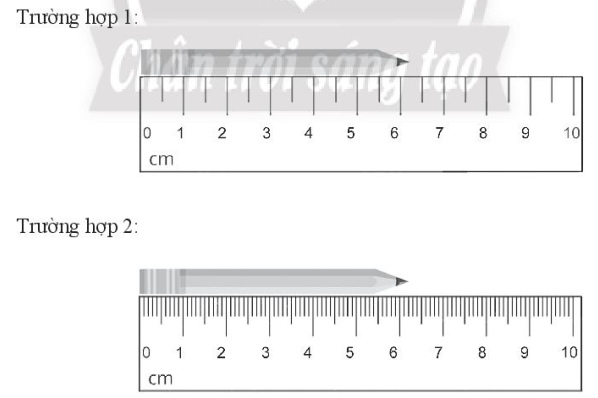
\includegraphics[width=0.6\linewidth]{../figs/VN10-2022-PH-TP003-P-2}
	\end{center}

}
\hideall{
\begin{itemize}
	\item Trường hợp 1: $\ell=\xsi{6,0\pm0,3}{\centi\meter}$.
	\item Trường hợp 2: $\ell=\xsi{6,20\pm0,05}{\centi\meter}$.
\end{itemize}
}
	
	\item \mkstar{3}
	
	{
		Đo chiều dày của một cuốn sách, được kết quả: $\SI{2,3}{cm}$; $\SI{2,4}{cm}$; $\SI{2,5}{cm}$; $\SI{2,4}{cm}$. Tính giá trị trung bình chiều dày cuốn sách. Sai số tuyệt đối trung bình của phép đo này là bao nhiêu?
	}
	
	\hideall{
		
		Ta có: 
		
		$$\overline{A} = \dfrac{A_1 + A_2 +...+ A_n}{n} =\SI{2,4}{cm}.$$
		
		Vậy trung bình chiều dày cuốn sách là $\SI{2,4}{cm}.$
		
		$$\Delta A_1 = |\overline{A} - A_1| = \text{0,1}.$$
		
		$$\Delta A_2 = |\overline{A} - A_2| = 0.$$
		
		$$\Delta A_3 = |\overline{A} - A_3| = \text{0,1}.$$
		
		$$\Delta A_4 = |\overline{A} - A_4| = 0.$$
		
		Ta có:
		
		$$\Delta \overline{A} = \dfrac{\Delta A_1 + \Delta A_2 +\Delta A_3+ \Delta A_4}{4} =\SI{0,05}{cm}.$$
		
		Vậy sai số tuyệt đối trung bình là $\SI{0,05}{cm}.$
	}
	
	\item \mkstar{3}
	
	{
		
		Bảng ghi thời gian một vật rơi giữa hai điểm cố định:
		
		\begin{center}
			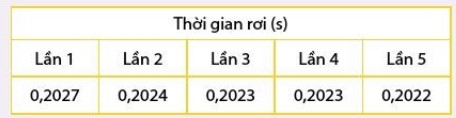
\includegraphics[scale=1]{../figs/VN10-2022-PH-TP003-1.jpg}
		\end{center}
		\begin{enumerate}[label=\alph*)]
			\item Tính giá trị trung bình của thời gian rơi.
			\item Tìm sai số tuyệt đối trung bình.
		\end{enumerate}
	}
	
	\hideall{
		
		\begin{enumerate}[label=\alph*)]
			\item Giá trị trung bình của thời gian rơi là:
			
			$$\dfrac{\text{0,2027} + \text{0,2024}+ \text{0,2023}+ \text{0,2023}+ \text{0,2022}}{5} \approx \text{0,2024}$$
			
			\item Sai số tuyệt đối:
			
			$$A_1= |\text{0,2024} - \text{0,2027}| = \text{0,0003}.$$
			
			$$A_2= |\text{0,2024} - \text{0,2024}| = \text{0,0000}.$$
			
			$$A_3= |\text{0,2024} - \text{0,2023}| = \text{0,0001}.$$
			
			$$A_4= |\text{0,2024} - \text{0,2023}| = \text{0,0001}.$$
			
			$$A_5= |\text{0,2024} - \text{0,2022}| = \text{0,0002}.$$
			
			Sai số tuyệt đối trung bình là: 
			
			$$\dfrac{\text{0,0003} + \text{0,0000} + \text{0,0001} + \text{0,0001}  + \text{0,0002}}{5} = \text{0,00014}.$$	\end{enumerate}
		
	}

	
	\item \mkstar{3}\\
	Dùng một đồng hồ đo thời gian có độ chia nhỏ nhất là $\SI{0.001}{\second}$ để đo $n$ lần thời gian rơi tự do của một vật bắt đầu từ điểm A đến điểm B. Kết quả đo hiển thị trong bảng sau:
	\begin{center}
		\begin{tabular}{|C{5em}|C{5em}|C{5em}|}
			\hline
			\thead{n} & \thead{\xsi{t}{\left(\second\right)}} &\thead{$\Delta t_i$}\\
			\hline
			1 & 0,398 &\\
			\hline
			2 & 0,399 &\\
			\hline
			3 & 0,408 & \\
			\hline
			4 & 0,410 &\\
			\hline
			5 & 0,406&\\
			\hline
			6 & 0,405 &\\
			\hline
			\thead{Trung bình} & &\\
			\hline
		\end{tabular}
	\end{center}
Hãy tính thời gian rơi trung bình, sai số ngẫu nhiên, sai số dụng cụ và sai số phép đo thời gian. Phép đo này là phép đo trực tiếp hay gián tiếp?
\hideall{
	\begin{center}
	\begin{tabular}{|C{5em}|C{5em}|C{5em}|}
		\hline
		\thead{n} & \thead{\xsi{t}{\left(\second\right)}} &\thead{$\Delta t_i$}\\
		\hline
		1 & 0,398 & 0,0063\\
		\hline
		2 & 0,399 &0,0053\\
		\hline
		3 & 0,408 & 0,0037\\
		\hline
		4 & 0,410 &0,0057\\
		\hline
		5 & 0,406&0,0017\\
		\hline
		6 & 0,405 &0,0007\\
		\hline
		\thead{Trung bình} &0,4043 &0,0039\\
		\hline	
	\end{tabular}
\end{center}
\begin{itemize}
	\item Thời gian rơi trung bình: $\overline{t}=\SI{0.4043}{\second}$.
	\item Sai số dụng cụ: $\Delta t_\text{dc}=\dfrac{\text{ĐCNN}}{2}=\SI{0.0005}{\second}$.
	\item Sai số ngẫu nhiên: $\overline{\Delta t}=\SI{0.0039}{\second}$.
	\item Sai số phép đo thời gian: $\Delta t=\overline{\Delta t}+\Delta t_\text{dc}=\SI{0.0044}{\second}$.
\end{itemize}
}
	

	\item \mkstar{4}
	
	
	{
		Dùng thước kẹp có ĐCNN $\SI{0,1}{mm}$ để đo 5 lần đường kính $d$ và chiều cao $h$ của một trụ thép, cho kết quả như trong bảng sau:
		
		\begin{center}
			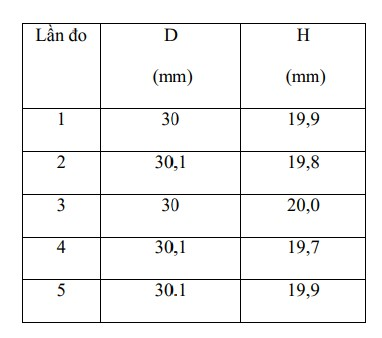
\includegraphics[scale=1]{../figs/VN10-2022-PH-TP003-8.jpg}
		\end{center}
		
		Hãy cho biết kết quả phép đo $d, h$ và tính thể tích trụ thép.
	}
	
	\hideall
	{	
		Phép đo $d, h$ là phép đo trực tiếp, giá trị
		trung bình và sai số ngẫu nhiên tính trong
		bảng sau
		
		\begin{center}
			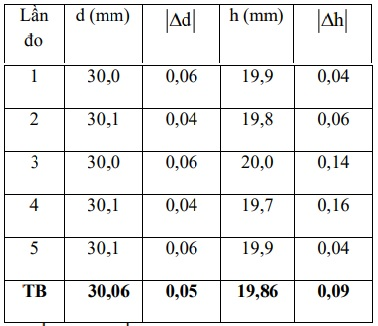
\includegraphics[scale=1]{../figs/VN10-2022-PH-TP003-9.jpg}
		\end{center}
		
		Sai số dụng cụ bằng $\SI{0,1}{mm}$. Vậy:
		
		Sai số phép đo đường kính trụ là:
		
		$$\Delta d = \text{0,05} + \text{0,05} =\SI{0,10}{mm}.$$
		
		Sai số phép đo chiều cao trụ là:
		
		$$\Delta h = \text{0,09} + \text{0,05} =\SI{0,14}{mm}.$$
		
		Kết quả: 
		
		$$d = \text{30,06} \pm \text{0,10}\ (\text{mm}).$$
		
		$$h = \text{19,86} \pm \text{0,14}\ (\text{mm}).$$
		
		Thể tích trung bình của khối trụ:
		
		$$\overline{V}  = \dfrac{\pi \bar{d}^2 \bar{h}}{4} =\SI{14094.42}{mm}^3.$$
		
		Sai số tỉ đối:
		
		$$\dfrac{\Delta V}{\overline V} = 2 \dfrac{\overline{\Delta d}}{\overline d} + \dfrac{\overline {\Delta h}}{\overline{h}} + \dfrac{\Delta \pi}{\pi} = \text{0,014} = 1,4\%.$$
		
		Sai số tuyệt đối:
		
		$$\Delta V = \overline{V} \delta V = \SI{193.13}{mm}^3.$$
		
		Suy ra:
		
		$$V = 14094 \pm 193 \ \text{mm}^3.$$
		
		
	}
	
\end{enumerate}		
%			\stopMyChapterToc
%		\mychapter[Ôn tập chương 1]{Ôn tập chương 1}
%			\startMyChapterToc	
%				\let\lesson\undefined
\newcommand{\lesson}{\phantomlesson{Bài 3.}}


\setcounter{section}{0}
\begin{enumerate}[label=\bfseries Bài \arabic*:,leftmargin=1.5cm]
	\item\mkstar{2}\\
	{Tìm số CSCN của các số sau:
		\begin{enumerate}[label=\alph*)]
			\item $78,9\pm 0,2$;
			\item $3,788\cdot10^9$;
			\item $2,46\cdot10^6$;
			\item $0,0053$.
		\end{enumerate}
}
	\hideall{
	\begin{enumerate}[label=\alph*)]
		\item 3 CSCN;
		\item 4 CSCN;
		\item 3 CSCN;
		\item 2 CSCN.
	\end{enumerate}
}
	\item \mkstar{3}\\
	{Trong quá trình thực hành tại phòng thí nghiệm, một bạn học sinh vô tình làm vỡ nhiệt kế thuỷ ngân và làm thuỷ ngân đổ ra ngoài như Hình \ref{fig:2P-2}. Em hãy giúp bạn học sinh đó đưa ra cách xử lí thuỷ ngân đổ ra ngoài đúng cách để đảm bảo an toàn.
		\begin{center}
			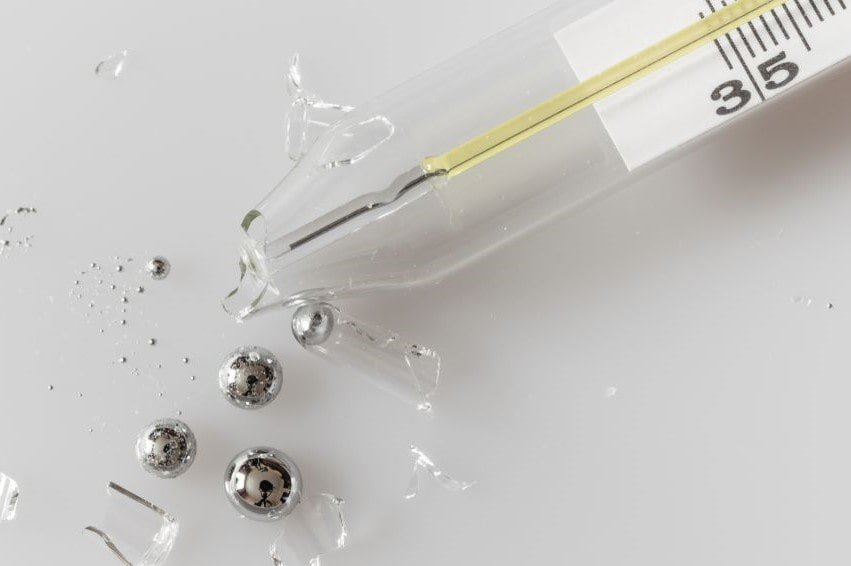
\includegraphics[width=0.3\linewidth]{../figs/VN10-2022-PH-TP002-P-2}
			\captionof{figure}{Thuỷ ngân bị đổ ra khỏi nhiệt kế}
			\label{fig:2P-2}
		\end{center}
	}
	\hideall{
		Cách xử lí đúng nguyên tắc an toàn: báo cho giáo viên tại phòng thí nghiệm, sơ tán các bạn học sinh ở khu vực gần đó, tắt quạt và đóng hết cửa sổ để tránh việc thuỷ ngân phát tán trong không khí. Người dọn dẹp phải sử dụng găng tay và khẩu trang để dọn sạch thuỷ ngân, tuyệt đối không được tiếp xúc với thuỷ ngân bằng tay trần.
	}
	
	\item \mkstar{3}\\
	{Theo em, tốc độ bay hơi của nước phụ thuộc vào những đặc điểm nào? Hãy dựa trên những hiện tượng thường thấy hằng ngày để đưa ra giả thuyết và thiết kế phương án thí nghiệm kiểm tra giải thuyết của mình.
	}
	\hideall{
		Nhiệt độ của nước, gió trên mặt thoáng của nước và diện tích mặt thoáng của nước.
	}
	
	\item \mkstar{3}\\
	{Hai người cùng đo chiều dài của cánh cửa sổ, kết quả thu được như sau:
		\begin{itemize}
			\item Người thứ nhất: $d=\xsi{120\pm1}{\centi\meter}$;
			\item Người thứ hai: $d=\xsi{120\pm 2}{\centi\meter}$;
		\end{itemize}
	Trong hai người, ai là người đo chính xác hơn? Vì sao?
}
	\hideall{
Người 1 đo chính xác hơn vì với cùng một giá trị trung bình nhưng sai số tuyệt đối trong phép đo của người 1 bé hơn sai số tuyệt đối trong phép đo của người 2.\\
Hoặc có thể tính sai số tỉ đối $\delta_1=\SI{0.83}{\percent}$ và $\delta_2=\SI{1.67}{\percent}$. Vì $\delta_1<\delta_2$ nên người 1 đo chính xác hơn.	
}
	
	\item \mkstar{3}\\
	{Một tấm bìa hình chữ nhật có chiều dài $\xsi{\left(21,3\pm0,2\right)}{\centi\meter}$ và chiều rộng $\xsi{\left(9,8\pm0,1\right)}{\centi\meter}$. Tính diện tích của tấm bìa.
	
}
\hideall{
$$S=\xsi{\left(21,3\pm0,2\right)\times\left(9,8\pm0,1\right)}{\centi\meter^2}=\xsi{\left(21,3\times 9,8 \pm 21,3\times 0,1 \pm 9,8\times 0,2 \pm 0,1\times 0,2\right)}{\centi\meter^2}= \xsi{\left(209\pm4\right)}{\centi\meter^2}.$$
Hoặc
$$\overline{S}=\overline{d}\times \overline{r}=\xsi{\left(21,3\times 9,8\right)}{\centi\meter^2}=\SI{208.8}{\centi\meter^2}$$
$$\Delta S=\left(\dfrac{\Delta d}{\overline{d}}+\dfrac{\Delta r}{\overline{r}}\right)\times \overline{S}=\SI{4.1}{\centi\meter^2}$$
Vậy kết quả đo diện tích của tấm bìa $S=\xsi{\left(209\pm4\right)}{\centi\meter^2}.$
}

\item \mkstar{3}\\
{Một học sinh đo cường độ dòng điện đi qua các đèn $\text{Đ}_1$ và $\text{Đ}_2$ như Hình \ref{fig:0001-1} được các giá trị lần lượt là 
	\begin{center}
		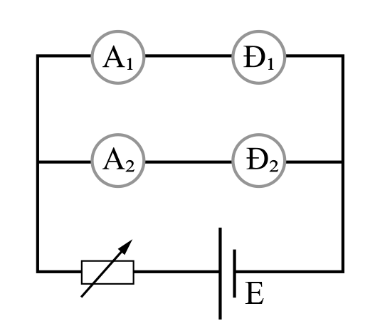
\includegraphics[width=0.3\linewidth]{../figs/VN10-2023-PH-TP0001-1}
		\captionof{figure}{}
		\label{fig:0001-1}
	\end{center}
	$$I_1=\xsi{\left(2,0\pm0,1\right)}{\ampere}$$
	$$I_2=\xsi{\left(1,5\pm0,2\right)}{\ampere}$$
	Cường độ dòng điện mạch chính được cho bởi
	$$I=I_1+I_2$$
	Tính giá trị và viết kết quả của $I$.


}
\hideall{
$$I=\xsi{\left(3,5\pm0,3\right)}{\ampere}.$$
}

\item \mkstar{3}\\
{Một nhóm học sinh đo được hiệu điện thế giữa hai đầu một điện trở là $\xsi{\left(10,0\pm0,3\right)}{\volt}$ và cường độ dòng điện qua điện trở là $\xsi{\left(1,3\pm0,2\right)}{\ampere}$. Viết kết quả tính giá trị của điện trở.

}
\hideall{
	Ta có: $R=\dfrac{U}{I}$\\
	Giá trị trung bình $$\overline{R}=\dfrac{\overline{U}}{\overline{I}}=\SI{7.7}{\ohm}$$
	Sai số tuyệt đối:
	$$\Delta R =\left(\dfrac{\Delta U}{\overline{U}}+\dfrac{\Delta I}{\overline{I}}\right)\cdot\overline{R}=\SI{1.4}{\ohm}$$
Vậy kết quả tính giá trị điện trở $R=\xsi{\left(7,7\pm1,4\right)}{\ohm}.$
}

\item \mkstar{3}\\
{Cho bảng số liệu thể hiện kết quả đo khối lượng của một túi trái cây bằng cân đồng hồ. Em hãy xác định sai số tuyệt đối ứng với từng lần đo, sai số tuyệt đối và sai số tương đối của phép đo. Biết sai số dụng cụ là $\SI{0.1}{\kilogram}$.
	\begin{center}
		\begin{tabular}{|c|c|c|}
			\hline
			\thead{Lần đo} & \thead{$\xsi{m}{\left(\kilogram\right)}$} & \thead{$\xsi{\Delta m}{\left(\kilogram\right)}$}\\
			\hline
			1& $4,2$ & \dots\\
			\hline
			2& $4,4$ & \dots\\
			\hline
			3& $4,4$ & \dots\\
			\hline
			4& $4,2$ & \dots\\
			\hline
		\end{tabular}
	\end{center}
}
\hideall{
	\begin{center}
		\begin{tabular}{|c|c|c|}
			\hline
			\thead{Lần đo} & \thead{$\xsi{m}{\left(\kilogram\right)}$} & \thead{$\xsi{\Delta m}{\left(\kilogram\right)}$}\\
			\hline
			1& $4,2$ & $0,1$\\
			\hline
			2& $4,4$ & $0,1$\\
			\hline
			3& $4,4$ & $0,1$\\
			\hline
			4& $4,2$ & $0,1$\\
			\hline
			Trung bình &$4,3$ & $0,1$\\
			\hline
		\end{tabular}
	\end{center}
Sai số tuyệt đối: $\Delta m=\overline{\Delta m}+\Delta m_\text{dc}=\SI{0.2}{\kilogram}$.\\
Sai số tương đối: $\delta m=\dfrac{\Delta m}{\overline{m}}=\SI{4.65}{\percent}$.\\
Kết quả đo: $m=\overline{m}\pm \Delta m=\xsi{4,3\pm0,2}{\kilogram}$.
}
\item \mkstar{4}\\
{Giá trị đo gia tốc rơi tự do $g$ có thể được xác định bằng cách đo chu kì dao động của con lắc đơn có chiều dài $\ell$. Mối quan hệ giữa $g, T$ và $\ell$ là 
	$$g=4\pi^2\left(\dfrac{\ell}{T^2}\right)$$
Trong một thí nghiệm, đo được:
$$\ell=\xsi{\left(0,55\pm0,02\right)}{\meter}; T=\xsi{\left(1,50\pm0,02\right)}{\second}$$
Tìm giá trị và viết kết quả của $g$.

}
\hideall{
	Giá trị trung bình:
	$$\overline{g}=4\pi^2\cdot\dfrac{\overline{\ell}}{\overline{T}^2}$$
	Sai số tuyệt đối
	$$\Delta g=\left(\dfrac{\Delta \ell}{\overline{\ell}}+2\cdot\dfrac{\Delta T}{\overline{T}}\right)\cdot\overline{g}=\SI{0.6}{\meter/\second^2}$$
	Kết quả đo:
$$g=\xsi{\left(9,7\pm0,6\right)}{\meter/\second^2}.$$

}
 \item \mkstar{4}\\
 {Một học sinh dùng thước có ĐCNN là $\SI{1}{\milli\meter}$ và một đồng hồ đo thời gian có ĐCNN $\SI{0.01}{\second}$ để đo 5 lần thời gian chuyển động của một chiếc xe đồ chơi chạy bằng pin từ điểm $A$ đến điểm $B$. Kết quả đo được cho ở bảng sau
 	\begin{center}
 		\begin{tabular}{|c|c|c|c|c|}
 			\hline
 			\thead{Lần đo}& \thead{$\xsi{s}{\left(\meter\right)}$} &\thead{$\xsi{\Delta s}{\left(\meter\right)}$} & \thead{$\xsi{t}{\left(\second\right)}$} & \thead{$\xsi{\Delta t}{\left(\second\right)}$}\\
 			\hline
 			1 & $0,546$ & \dots & $2,47$ & \dots\\
 			\hline
 			2 & $0,554$ & \dots & $2,51$ & \dots\\
 			\hline
 			3 & $0,549$ & \dots & $2,42$ & \dots\\
 			\hline
 			4 & $0,560$ & \dots & $2,52$ & \dots\\
 			\hline
 			5 & $0,551$ & \dots & $2,48$ & \dots\\
 			\hline
 		\end{tabular}
 	\end{center}
 \begin{enumerate}[label=\alph*)]
 	\item Nêu nguyên nhân gây ra sự sai khác giữa các lần đo?
 	\item Tính sai số tuyệt đối và sai số tỉ đối của phép đo $s$, $t$.
 	\item Biểu diễn kết quả đo $s$ và $t$.
 	\item Tính sai sối tỉ đối $\delta v$ sai số tuyệt đối $\Delta v$. Biểu diễn kết quả tính $v$.
 \end{enumerate}
}
\hideall{
\begin{enumerate}[label=\alph*)]
	\item Nguyên nhân gây ra sai khác giữa các lần đo: Do cấu tạo của dụng cụ thí nghiệm, thao tác khi đo chưa chuẩn xác.
	\item $\Delta s=\SI{0.0055}{\meter}$; $\Delta t=\SI{0.035}{\second}$.
	\item $s=\xsi{0,5520\pm0,0055}{\meter}$; $t=\xsi{2,480\pm0,035}{\second}$.
	\item $\delta v=\SI{2.41}{\percent}$; $\Delta v=\SI{0.0054}{\meter/\second}$.\\
	Kết quả tính: $v=\xsi{0,2226\pm0,0054}{\meter/\second}$.
\end{enumerate}
}

\end{enumerate}
%			\stopMyChapterToc
%		\stopPartToc
%	\part{Mô tả chuyển động}
%	\setcounter{mychapter}{3}
%		\startPartToc
%		\mychapter[Chuyển động thẳng]{Chuyển động thẳng}
%			\startMyChapterToc
%				\let\lesson\undefined
\newcommand{\lesson}{\phantomlesson{Bài 4: Chuyển động thẳng}}
\chapter[Độ dịch chuyển và quãng đường]{Độ dịch chuyển và quãng đường đi được}
\setcounter{section}{0}
\section{Lý thuyết}
\subsection{Chuyển động cơ. Chất điểm}
\subsubsection{Chuyển động cơ}
Chuyển động cơ của một vật (gọi tắt là chuyển động) là sự thay đổi vị trí của vật đó so với các vật khác theo thời gian.
\subsubsection{Chất điểm}
Một vật chuyển động được coi là một chất điểm nếu kích thước của nó rất nhỏ so với độ dài đường đi (hoặc so với những khoảng cách mà ta đề cập đến).

Ví dụ: trong chuyển động của ô tô từ thành phố Hồ Chí Minh đến Hà Nội thì ô tô được xem là chất điểm.
\subsubsection{Quỹ đạo}
Tập hợp tất cả các vị trí của một chất điểm chuyển động tạo ra một đường trong không gian, đường đó gọi là quỹ đạo của chuyển động.
\subsection{Cách xác định vị trí của vật trong không gian}
\subsubsection{Vật làm mốc và thước đo}
Nếu đã biết đường đi (quỹ đạo) của vật, ta cần chọn một vật làm mốc và một chiều dương trên đường đi, và dùng thước đo chiều dài đoạn đường từ vật làm mốc đến vật là có thể xác định được chính xác vị trí của vật.
\begin{center}
	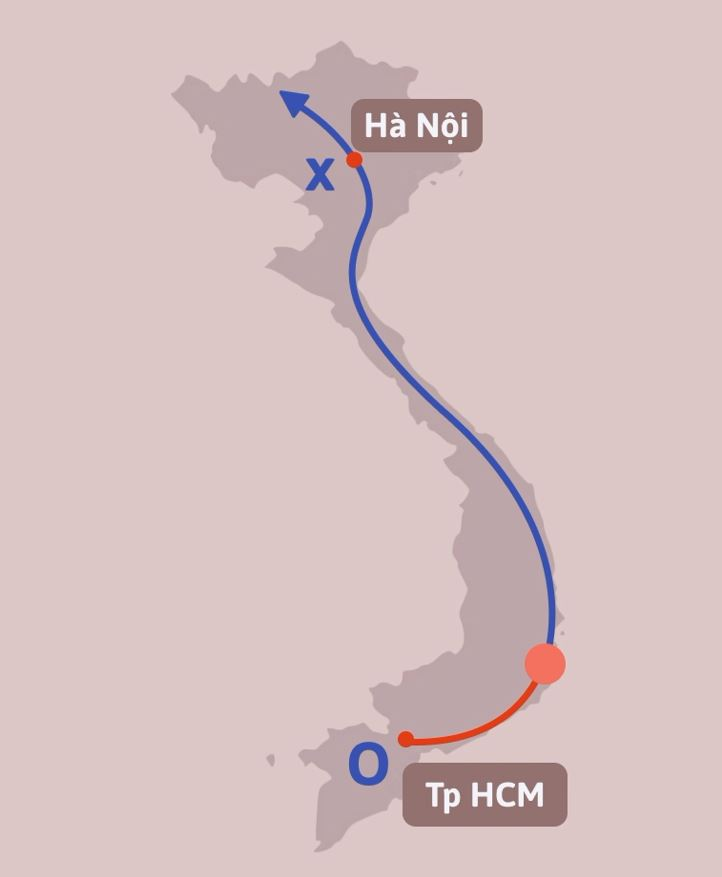
\includegraphics[scale=0.3]{../figs/VN10-PH-02-L-001-1-V2-01.jpg}
\end{center}
\subsubsection{Hệ tọa độ}
Muốn xác định vị trí của một điểm trên một mặt phẳng ta cần có hệ tọa độ với hai trục O$x$ và O$y$ vuông góc nhau, hình chiếu vuông góc của điểm xuống hai trục tọa độ đó chính là tọa độ của điểm đó.
\begin{center}
	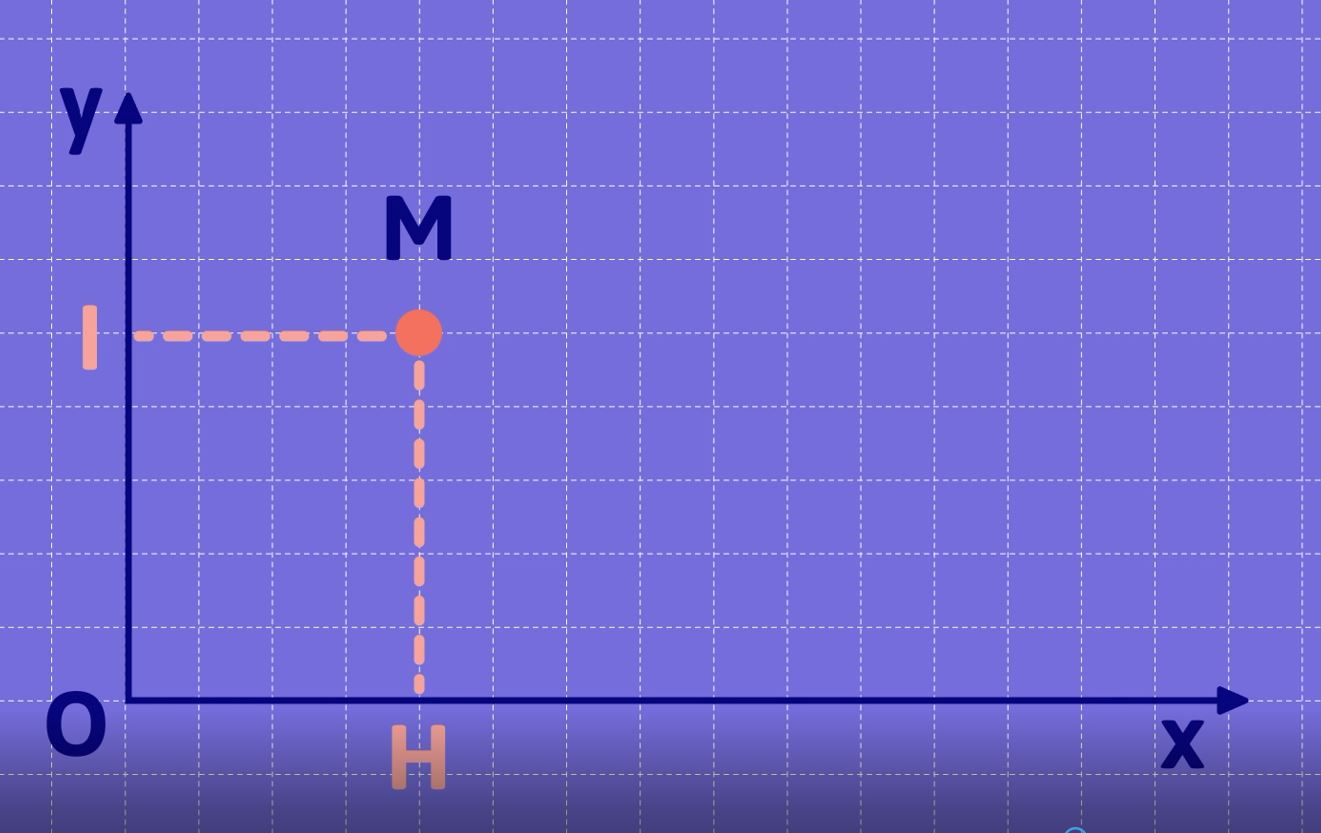
\includegraphics[height=3cm]{../figs/VN10-PH-02-L-001-1-V2-02.jpg}
	
\end{center}
\subsection{Cách xác định thời gian trong chuyển động}
\subsubsection{Mốc thời gian và đồng hồ}
Để mô tả chuyển động của một vật ta phải biết tọa độ của vật đó ở những thời điểm khác nhau. Muốn thế, ta phải chỉ rõ mốc thời gian và đo khoảng thời gian trôi đi kể từ mốc thời gian bằng một đồng hồ.
\subsubsection{Thời điểm và thời gian}
Nếu lấy mốc thời gian là thời điểm vật bắt đầu chuyển động (thời điểm 0) thì số chỉ của thời điểm sẽ trùng với số đo khoảng thời gian đã trôi qua kể từ mốc thời gian.
\subsection{Hệ quy chiếu}
Một hệ quy chiếu gồm:
\begin{itemize}
	\item mốc tọa độ và một hệ tọa độ để đo vị trí;
	\item mốc thời gian và một đồng hồ để xác định thời điểm.
\end{itemize}
\subsection{Độ dịch chuyển và quãng đường đi được}
\subsubsection{Độ dịch chuyển}
Độ dịch chuyển được xác định bằng độ biến thiên toạ độ của vật
$$d=x_2-x_1=\Delta x$$
\begin{center}
	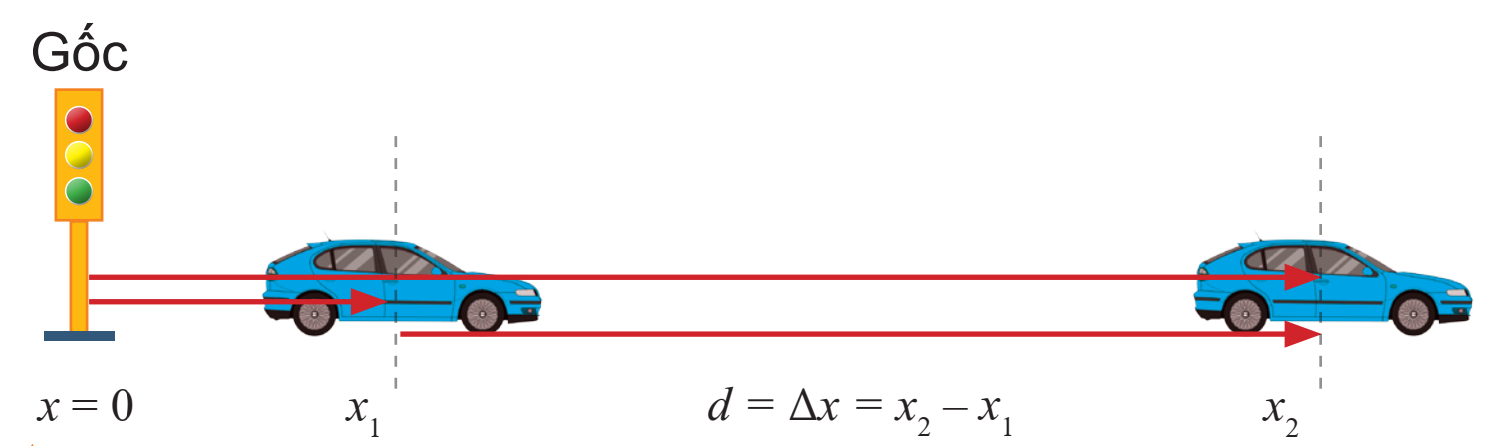
\includegraphics[width=0.6\linewidth]{../figs/VN10-2023-PH-TP004-1}
	\captionof{figure}{Ví dụ thực tế về độ dịch chuyển của vật trên đường thẳng}
\end{center}
Độ dịch chuyển có các đặc điểm sau:
\begin{itemize}
	\item độ dịch chuyển là một đại lượng vectơ $\left(\vec{d}\right)$ có gốc tại vị trí ban đầu, hướng từ vị trí đầu đến vị trí cuối, độ lớn bằng khoảng cách giữa vị trí đầu và vị trí cuối.
	\item độ dịch chuyển là một đại lượng có thể nhận giá trị dương, âm hoặc bằng không. 
\end{itemize}
\subsubsection{So sánh độ dịch chuyển và quãng đường đi được}
\begin{longtable}{|m{20em}|m{20em}|}
	\hline
	\thead{Độ dịch chuyển $\left(\vec{d}\right)$} & \thead{Quãng đường $\left(s\right)$}\\
	\hline
	Là đại lượng vectơ. & Là đại lượng vô hướng.\\
	\hline
	Cho biết sự thay đổi vị trí của một vật (về hướng và độ dời). & Cho biết độ dài mà vật đi được.\\
	\hline
	Có thể nhận giá trị dương, âm hoặc bằng 0. & Có giá trị không âm.\\
	\hline
\end{longtable}
\luuy{Khi vật chuyển động theo một hướng (chuyển động thẳng và không đổi chiều) thì độ lớn của độ dịch chuyển và quãng đường đi được bằng nhau $(d=s)$.

}
\section{Mục tiêu bài học - Ví dụ minh họa}
\begin{dang}{Thực hiện xác định thời điểm và thời gian (mốc thời gian và đồng hồ)}
	\viduii{2}{Giờ Berlin chậm hơn giờ Hà Nội 5 giờ. Trận bóng đá diễn ra tại Beclin lúc 19h00 ngày 2-9-2021. Khi đó theo giờ Hà Nội là
		\begin{mcq}(2)
			\item 14h00 ngày 3-9-2021.
			\item 0h00 ngày 3-9-2021. 
			\item 0h00 ngày 2-9-2021
			\item 14h00 ngày 2-9-2021.
		\end{mcq}
	}
	{\hide{	
		Giờ Berlin chậm hơn giờ Hà Nội 5 giờ, nghĩa là
		$$t_{\text{B}}+\SI{5}{\hour}=t_{\text{HN}}.$$
		Trận bóng đá diễn ra tại Berlin lúc 19h00 ngày 2-9-2021. Thời điểm đó theo giờ Hà Nội là:
		$$t_{\text{HN}}=t_{\text{B}}+\SI{5}{\hour}=19\text{h}00 + 5\text{h} = 24\text{h}00$$
		Một ngày chỉ có 24 giờ nên thời điểm trên đã bước sang ngày hôm sau. Do đó, trận bóng trên diễn ra vào lúc 0h00 ngày 3-9-2007 giờ Hà Nội. 	
		
		\textbf{Đáp án: B}.
	}}

	\viduii{3}{Theo lịch trình tại bến xe ở Hà Nội thì ô tô chở khách trên tuyến Hà Nội - Hải Phòng chạy từ Hà Nội lúc 6 giờ sáng, đi qua Hải Dương lúc 7 giờ 15 phút sáng và tới Hải Phòng lúc 8 giờ 50 phút sáng cùng ngày. Hà Nội cách Hải Dương 60 km và cách Hải Phòng $\SI{105}{km}$. Xe ô tô chạy liên tục không nghỉ dọc đường, chỉ dừng lại 10 phút tại bến xe Hải Dương để đón, trả khách. Tính khoảng thời gian chuyển động và quãng đường đi được của các hành khách sau:
		\begin{enumerate}[label=\alph*)]
			\item Hành khách lên xe tại Hà Nội đi Hải Phòng.
			\item Hành khách lên xe tại Hải Dương đi Hải Phòng.
		\end{enumerate}
	}
	{\hide{
		\begin{enumerate}[label=\alph*)]
			\item Đối với hành khách lên xe tại Hà Nội đi Hải Phòng, chọn bến xe Hà Nội làm mốc và thời điểm ô tô bắt đầu xuất phát là mốc thời gian.
			
			Khoảng thời gian chuyển động là:	
			\begin{center}
				(8 giờ 50 phút - 6 giờ) - 10 phút = 2 giờ 40 phút.
			\end{center}
			Quãng đường đi được đúng bằng độ dài của đoạn đường Hà Nội - Hải Phòng là $\SI{105}{km}$.
			\item Đối với hành khách lên xe tại Hải Dương đi Hải Phòng, chọn bến xe Hải Dương làm mốc và thời điểm ô tô bắt đầu xuất phát là mốc thời gian.
			
			Khoảng thời gian chuyển động là:
			\begin{center}
				8 giờ 50 phút - (7 giờ 15 phút + 10 phút) = 1 giờ 25 phút.
			\end{center}
			Quãng đường đi được là:
			$$\SI{105}{km}-\SI{60}{km}=\SI{45}{km}.$$
		\end{enumerate}
	}}
\end{dang}

\begin{dang}{So sánh được quãng đường đi được và độ dịch chuyển.}
	\viduii{2}
{Xét quãng đường $AB$ dài $\SI{1000}{\meter}$ với $A$ là vị trí nhà của em và $B$ là vị trí của bưu điện. Tiệm tạp hóa nằm tại vị trí $C$ là trung điểm của $AB$. Nếu chọn nhà em làm gốc tọa độ và chiều dương hướng từ nhà em đến bưu điện. Hãy xác định độ dịch chuyển và quãng đường đi được của em trong các trường hợp:
	\begin{center}
		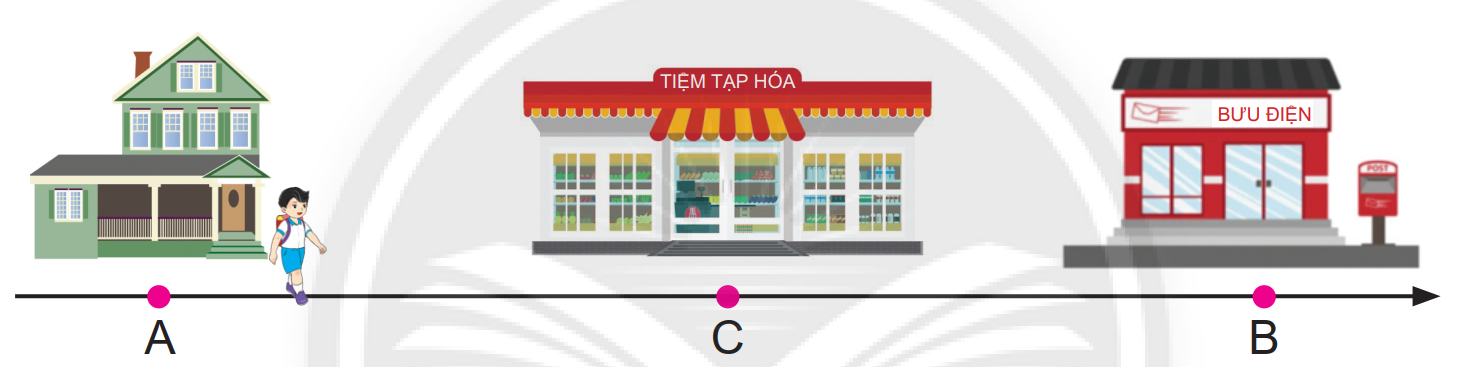
\includegraphics[width=0.6\linewidth]{../figs/VN10-2023-PH-TP004-2}
	\end{center}
	\begin{enumerate}[label=\alph*)]
		\item Đi từ nhà đến bưu điện.
		\item Đi từ nhà đến bưu điện rồi quay lại tiệm tạp hóa.
		\item Đi từ nhà đến tiệm tạp hóa rồi quay về. 
	\end{enumerate}	
}
{\hide{
\begin{enumerate}[label=\alph*)]
	\item Độ dịch chuyển $d=AB=x_B-x_A=\SI{1000}{\meter}-\SI{0}{\meter}=\SI{1000}{\meter}$.\\
	Quãng đường đi được $s=AB=\SI{1000}{\meter}$.
	\item Độ dịch chuyển $d=AC=x_A-x_C=\SI{500}{\meter}-\SI{0}{\meter}=\SI{500}{\meter}$.\\
	Quãng đường đi được $s=AB+BC=\SI{1500}{\meter}$.
	\item  Độ dịch chuyển $d=x_A-x_A=\SI{0}{\meter}$.\\
	Quãng đường đi được $s=2AC=\SI{1000}{\meter}$.
\end{enumerate}
}}

\viduii{2}
{Một vận động viên chạy từ cổng Dinh Thống Nhất (A) đến Thảo Cầm Viên (D) theo hai quỹ đạo khác nhau. Hãy xác định độ dịch chuyển và quãng đường chạy được của người vận động viên trong 2 trường hợp trên.
\begin{center}
	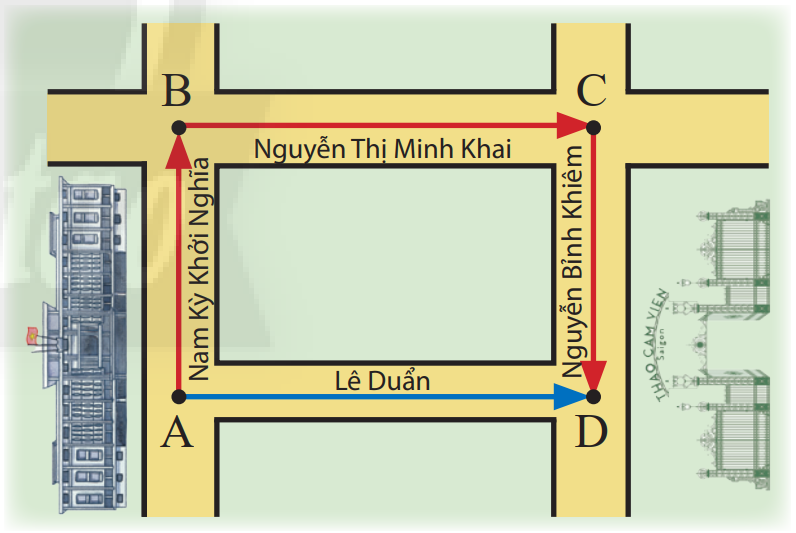
\includegraphics[width=0.5\linewidth]{../figs/VN10-2023-PH-TP004-3}
\end{center}
}
{\hide{
\textbf{Trường hợp 1:} Nếu vận động viên chạy theo đường Lê Duẩn thì\\
	Độ dời $\vec{d}=\overrightarrow{AD}$, về độ lớn thì $d=AD$.\\
	Quãng đường $s=AD$.\\
\textbf{Trường hợp 2:} Nếu vận động viên chạy theo đường Nam Kì Khởi Nghĩa qua đường Nguyễn Thị Minh Khai rồi mới đến Thảo Cầm Viên ở đường Nguyễn Bỉnh Khiêm thì\\
Độ dời $\vec{d}=\overrightarrow{AD}$, về độ lớn thì $d=AD$.\\
Quãng đường $s=AB+BC+CD$.
}}
\end{dang}


%				\let\lesson\undefined
\newcommand{\lesson}{\phantomlesson{Bài 4.}}


\setcounter{section}{2}
\section{Bài tập trắc nghiệm}
\begin{enumerate}[label=\bfseries Câu \arabic*:,leftmargin=1.5cm]
	\item \mkstar{1}\\
	{Hãy chọn câu phát biểu đúng?
	\begin{mcq}
		\item Hệ quy chiếu bao gồm hệ toạ độ, mốc thời gian và đồng hồ.
		\item Hệ quy chiếu bao gồm vật làm mốc, mốc thời gian và đồng hồ.
		\item Hệ quy chiếu bao gồm vật làm mốc, hệ toạ độ, mốc thời gian.
		\item Hệ quy chiếu bao gồm vật làm mốc, hệ toạ độ, mốc thời gian và đồng hồ.
	\end{mcq}
}
\hideall{
\textbf{Đáp án: D.}
}

\item \mkstar{1}\\
{Kết luận nào sau đây là đúng khi nói về độ dịch chuyển và quãng đường đi được của một vật?
	\begin{mcq}
		\item Độ dịch chuyển và quãng đường đi được đều là đại lượng vô hướng.
		\item Độ dịch chuyển là đại lượng vectơ còn quãng đường đi được là đại lượng vô hướng.
		\item Độ dịch chuyển và quãng đường đi được đều là đại lượng vectơ.
		\item Độ dịch chuyển và quãng đường đi được đều là đại lượng không âm.
	\end{mcq}
}
\hideall{
\textbf{Đáp án: B.}
}

\item\mkstar{2}\\
{Một vật bắt đầu chuyển động từ điểm $O$ đến điểm $A$, sau đó chuyển động về điểm $B$. Quãng đường và độ dịch chuyển của vật tương ứng là
	\begin{center}
		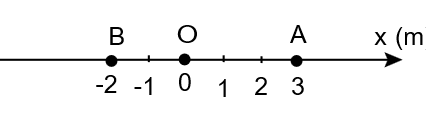
\includegraphics[width=0.4\linewidth]{../figs/VN10-2022-PH-TP004-P-2}
	\end{center}
\begin{mcq}(4)
	\item $\SI{2}{\meter}$; $\SI{-2}{\meter}$.
	\item $\SI{8}{\meter}$; $\SI{-2}{\meter}$.
	\item $\SI{2}{\meter}$; $\SI{2}{\meter}$.
	\item $\SI{8}{\meter}$; $\SI{-8}{\meter}$.
\end{mcq}
}
\hideall{
\textbf{Đáp án: B.}
}
\item \mkstar{2}\\
{Nếu nói “Trái Đất quay quanh Mặt Trời” thì trong câu nói này vật nào được chọn làm mốc
	\begin{mcq}(2)
		\item Cả Mặt Trời và Trái Đất.
		\item Trái Đất.
		\item Mặt Trăng.
		\item Mặt Trời.
	\end{mcq}
}
\hideall{
\textbf{Đáp án: D.}
}

\item \mkstar{2}\\
{“Lúc 15 giờ 30 phút hôm qua, xe chúng tôi đang chạy trên quốc lộ 5, cách Hải Dương 10 km”. Việc xác định vị trí của ô tô như trên còn thiếu yếu tố gì?
	\begin{mcq}(2)
		\item Vật làm mốc.
		\item Chiều dương trên đường đi.
		\item Mốc thời gian.
		\item Thước đo và đồng hồ.
	\end{mcq}
}
\hideall{
\textbf{Đáp án: B.}
}

\item \mkstar{2}\\
{Trong trường hợp nào dưới đây số chỉ thời điểm mà ta xét trùng với số đo khoảng thời gian trôi?
	\begin{mcq}
		\item Một trận bóng đá diễn ra từ 15 giờ đến 16 giờ 45 phút.
		\item Lúc 8 giờ một ô tô khởi hành từ Thành phố Hồ Chí Minh, sau 3 giờ chạy thì xe đến Vũng Tàu.
		\item Một đoàn tàu xuất phát từ Vinh lúc 0 giờ, đến 8 giờ 05 phút thì đoàn tàu đến Huế.
		\item Không có trường hợp nào phù hợp với yêu cầu nêu ra.
	\end{mcq}

}
\hideall{
\textbf{Đáp án: C.}
}


\item \mkstar{2}\\
{Bảng giờ tàu ở bên cho chúng ta biết quãng đường và thời gian mà đoàn tàu SE1 chạy từ ga Huế đến ga Sài Gòn (bỏ qua thời gian tàu đỗ lại các ga) tương ứng là
	\begin{center}
		\begin{tabular}{|c|c|c|}
			\hline
			\thead{Tên ga} & \thead{km} & \thead{SE1}\\
			\hline
			Hà Nội & 0 & 22:15\\
			\hline
			Thanh Hoá & 175& 01:28 (ngày $+1$)\\
			\hline
			Huế & 688 & 11:08 (ngày $+1$)\\
			\hline
			Sài Gòn & 1726 & 06:32 (ngày $+2$)\\
			\hline
		\end{tabular}
	\end{center}
	\begin{mcq}(2)
		\item $\SI{1726}{\kilo\meter}$, 4 giờ 36 phút.
		\item $\SI{1726}{\kilo\meter}$, 19 giờ 24 phút.
		\item $\SI{1038}{\kilo\meter}$, 19 giờ 24 phút.
		\item $\SI{1038}{\kilo\meter}$, 4 giờ 36 phút.
	\end{mcq}

}
\hideall{
\textbf{Đáp án: C.}
}

\item \mkstar{3}\\
{\begin{minipage}[l]{0.65\textwidth}
		Hai người đi xe đạp từ $A$ đến $C$, người thứ nhất đi theo đường từ $A$ đến $B$, rồi từ $B$ đến $C$; người thứ hai đi thẳng từ $A$ đến $C$. Cả hai đều về đích cùng một lúc.\\
		Hãy chọn kết luận \textbf{sai}.
		\begin{mcq}
			\item Người thứ nhất đi được quãng đường $\SI{8}{\kilo\meter}$.
			\item Độ dịch chuyển của người thứ nhất và người thứ hai bằng nhau.
			\item Độ dịch chuyển và quãng đường đi được của người thứ nhất bằng nhau.
			\item Độ dịch chuyển của người thứ nhất là $\SI{5.7}{\kilo\meter}$, hướng $\SI{45}{\degree}$ Đông – Bắc.
		\end{mcq}
	\end{minipage}
\begin{minipage}{0.35\textwidth}
	\begin{center}
		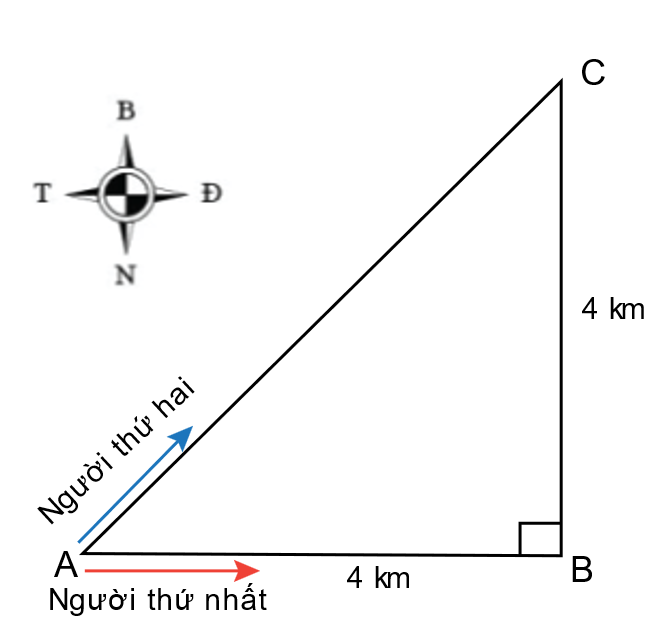
\includegraphics[width=0.7\linewidth]{../figs/VN10-2022-PH-TP004-P-3}
	\end{center}
\end{minipage}

}
\hideall{
\textbf{Đáp án: C.}
}

\item \mkstar{3}\\
{Cho biết Giờ Phối hợp Quốc Tế gọi tắt UTC. So với 0 giờ Quốc Tế, Việt Nam ở múi giờ thứ 7 (UTC+7) và Nhật Bản ở múi giờ thứ 9 (TUC+ 9). Ngày 20/12/2021, máy bay VN300, thuộc hãng hàng không Vietnam Airlines, khởi hành từ Tp. Hồ Chí Minh lúc 0 giờ 20 phút và đến Tp. Tokyo lúc 7 giờ 45 phút, theo giờ địa phương. Thời gian di chuyển của chuyến bay này là
\begin{mcq}(4)
	\item 5 giờ 25 phút.
	\item 9 giờ 25 phút.
	\item 7 giờ 25 phút.
	\item 8 giờ 05 phút.
\end{mcq}
}
\hideall{
\textbf{Đáp án: A.}
}
\item \mkstar{3}\\
{Chuyến bay từ Thành phố Hồ Chí Minh đi Paris khởi hành lúc 21 giờ 30 phút giờ Hà Nội ngày hôm trước, đến Paris lúc 5 giờ 30 phút sáng hôm sau theo giờ Paris. Biết giờ Paris chậm hơn giờ Hà Nội là 6 giờ. Theo giờ Hà Nội, máy bay đến Paris lúc
\begin{mcq}(4)
	\item 11 giờ 30 phút.
	\item 14 giờ.
	\item 12 giờ 30 phút.
	\item 10 giờ.
\end{mcq}
}
\hideall{
\textbf{Đáp án: A.}
}

\end{enumerate}
\section{Bài tập tự luận}
\begin{enumerate}[label=\bfseries Bài \arabic*:,leftmargin=1.5cm]
	\item \mkstar{1}
	
	
	{
		Khi nào quãng đường và độ di chuyển của một vật có cùng một độ lớn?
	}
	
	\hideall
	{	Chuyển động của vật có quỹ đạo là đường thẳng và không đổi chiều chuyển động.
	}

	\item \mkstar{2}
	
	
	{
		Xác định độ dịch chuyển trong các khoảng thời gian liên tiếp bằng nhau của mỗi chuyển động.
		
		\begin{center}
			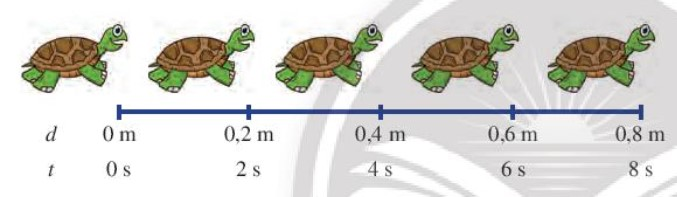
\includegraphics[scale=0.6]{../figs/VN10-2022-PH-TP004-6.jpg}
		\end{center}
	}
	
	\hideall
	{	
		
		Độ dịch chuyển trong các khoảng thời gian liên tiếp bằng nhau của mỗi chuyển động
		
		$$\Delta d_1 = x_2 - x_1 = \SI{0,2}{m}.$$
		
		$$\Delta d_2 = x_3 - x_2 = \SI{0,2}{m}.$$
		
		$$\Delta d_3 = x_4 - x_3 = \SI{0,2}{m}.$$
		
		$$\Delta d_4 = x_5 - x_4 = \SI{0,2}{m}.$$
		
	}


	\item \mkstar{2}
	
	
	{
		Hãy xác định các độ dịch chuyển mô tả ở hình trong tọa độ địa lí.
		
		\begin{center}
			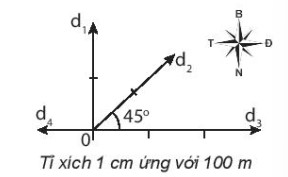
\includegraphics[scale=1]{../figs/VN10-2022-PH-TP004-2.jpg}
		\end{center}
	}
	
	\hideall
	{	
		Độ dịch chuyển mô tả trên hình là:
		
		$+ d_1 = \SI{200}{m}\ \text{(Bắc)}.$
		
		$+ d_2 = \SI{200}{m}\ \text{(Đông Bắc)}.$
		
		$+ d_3 = \SI{300}{m}\ \text{(Đông)}.$
		
		$+ d_4 = \SI{100}{m}\ \text{(Tây)}.$
		
		
	}

	\item \mkstar{2}
	
	
	{
		Một ô tô chuyển động trên đường thẳng. Tại thời điểm $t_1$, ô tô ở cách vị trí xuất phát $\SI{5}{km}$. Tại thời điểm $t_2$, ô tô cách vị trí xuất phát $\SI{12}{km}$. Từ $t_1$ đến $t_2$, độ dịch chuyển của ô tô đã thay đổi một đoạn bằng bao nhiêu?
		
	}
	
	\hideall
	{	
		Từ $t_1$ đến $t_2$ ,  độ dịch chuyển của ô tô thay đổi một đoạn bằng 
		
		$$12-5 = \SI{7}{km}.$$
	}
	\item \mkstar{2}\\
	{Một xe ô tô xuất phát từ tỉnh A, đi đến tỉnh B; rồi lại trở về vị trí xuất phát ở tỉnh A. Xe này đã dịch chuyển, so với vị trí xuất phát một đoạn bằng bao nhiêu? 
	}
	\hideall
	{Xe máy này đã dịch chuyển, so với vị trí xuất phát một đoạn là $\SI{0}{km}$.
	}

	\item \mkstar{2}\\
	{Xác định vị trí của vật A trên trục Ox ở hình vẽ tại thời điểm 12h. Biết vật chuyển động thẳng, mỗi giờ đi được $\SI{40}{km}$.
		
		\begin{center}
			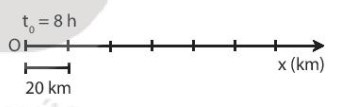
\includegraphics[scale=1]{../figs/VN10-2022-PH-TP004-1.jpg}
		\end{center}
	}
	\hideall
	{	Thời gian vật di chuyển là:
		
		$$12 - 8 = \SI{4}{h}.$$
		
		1 giờ vật di chuyển được $\SI{40}{km}$
		
		$\Rightarrow$ 4 giờ vật di chuyển được: 
		
		$$4 \cdot 40 = \SI{160}{km}.$$
		Tương ứng vật cách gốc toạ độ 8 ô đơn vị.
	}
	
	\item \mkstar{2}
	
	
	{
		Bạn A đi xe đạp từ nhà qua trạm xăng, tới siêu thị mua đồ rồi quay về nhà cất đồ, sau đó đi đến trường. 
		
		\begin{center}
			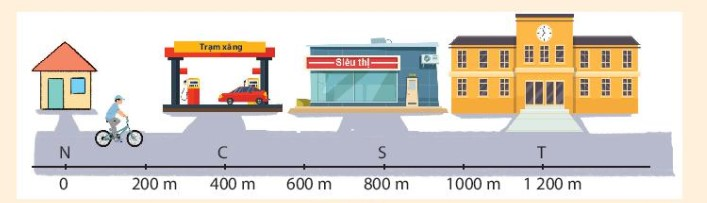
\includegraphics[scale=1]{../figs/VN10-2022-PH-TP004-4.jpg}
		\end{center}
		Chọn hệ tọa độ có gốc là vị trí nhà bạn A, trục Ox trùng với đường đi từ nhà bạn A đến trường. 
		\begin{enumerate}[label=\alph*)]
			\item Tính quãng đường đi được và độ dịch chuyển của bạn A khi đi từ trạm xăng tới siêu thị.
			\item Tính quãng đường đi được và độ dịch chuyển của bạn A trong cả chuyến đi trên.
		\end{enumerate}
	}
	
	\hideall
	{	
		\begin{enumerate}[label=\alph*)]
			\item Quãng đường bạn A đi từ trạm xăng đến siêu thị là: $$800 - 400 = \SI{400}{m}.$$
			
			Độ dịch chuyển của bạn A từ trạm xăng đến siêu thị là: $$800 - 400 = \SI{400}{m}.$$
			
			\item 
			Quãng đường đi được của bạn A trong cả chuyến đi:
			
			+ Quãng đường bạn A đi từ nhà đến siêu thị là: $\SI{800}{m}.$
			
			+ Quãng đường bạn A quay về nhà cất đồ là: $\SI{800}{m}.$
			
			+ Quãng đường bạn A đi từ nhà đến trường là: $\SI{1200}{m}.$
			
			$\Rightarrow$ Quãng đường đi được của bạn A trong cả chuyến đi là: 	$$ 800 \cdot 2 + 1200 = \SI{2800}{m}.$$ 
			
			Điểm đầu xuất phát của bạn A là nhà, điểm cuối của bạn A là trường.
			
			$\Rightarrow$ Độ dịch chuyển của bạn A là $\SI{1200}{m}.$
			
			
			Quãng đường đi được và độ dịch chuyển của A trong cả chuyến đi trên là khác nhau. 
			
		\end{enumerate}
	}
	
	\item \mkstar{2}
	
	
	{
		Hãy so sánh độ lớn của quãng đường đi được và độ dịch chuyển của ba chuyển động. 
		
		\begin{center}
			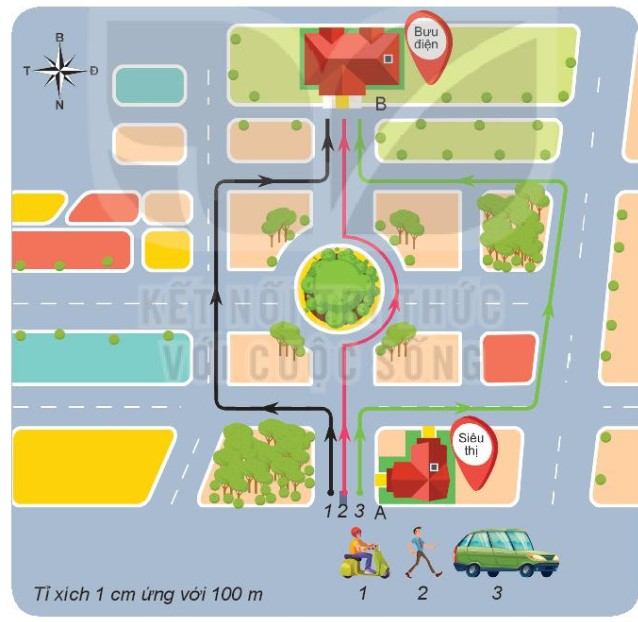
\includegraphics[scale=0.8]{../figs/VN10-2022-PH-TP004-3.jpg}
		\end{center}
	}
	
	\hideall
	{	
		Quãng đường đi được từ ngắn đến dài: $$2 - 1 - 3.$$
		
		Độ dịch chuyển, ta thấy điểm đầu và điểm cuối của ba chuyển động đều như nhau nên độ dịch chuyển của ba chuyển động bằng nhau.
		
	}
	
	
	\item \mkstar{2}
	
	
	{
		Một người lái ô tô đi thẳng $\SI{6}{km}$ theo hướng Tây, sau đó rẽ trái đi thẳng theo hướng Nam $\SI{4}{km}$ rồi quay sang hướng Đông $\SI{3}{km}$. Xác định quãng đường đi được và độ dịch chuyển của ô tô.
	}
	
	\hideall
	{	\begin{center}
			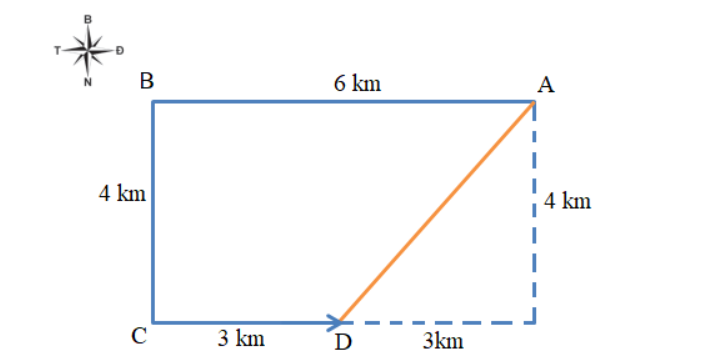
\includegraphics[width=0.4\linewidth]{../figs/VN10-2022-PH-TP004-P-1}
		\end{center}
		Quãng đường đi được :
		
		$$s=6+4+3=\SI{13}{km}.$$
		
		Độ dịch chuyển là :
		
		$$d=\sqrt{3^2+4^2}=\SI{5}{\kilo\meter}$$
	}
	
	
	
\item \mkstar{3}


{
	Một người bơi ngang từ bờ bên này sang bờ bên kia của một dòng sông rộng $\SI{50}{m}$ có dòng chảy theo hướng từ Bắc xuống Nam. Do nước sông chảy mạnh nên khi sang đến bờ bên kia thì người đó đã trôi xuôi theo dòng nước $\SI{50}{m}$. Xác định độ dịch chuyển của người đó.
}

\hideall
{
	\begin{center}
		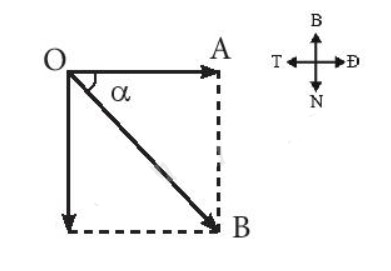
\includegraphics[scale=0.6]{../figs/VN10-2022-PH-TP0001-2.jpg}
	\end{center}
	Người bơi ngang từ bờ bên này sang bên kia theo dự định là OA = $\SI{50}{m}$.
	
	Thực tế, do nước sông chảy mạnh nên vị trí của người đó ở vị trí B, ta có AB = $\SI{50}{m}$.
	
	$\Rightarrow$ Độ dịch chuyển:
	
	$$\Rightarrow\text{OB} = \sqrt{\text{OA}^2 + \text{AB}^2} = \SI{70,7}{km}.$$ 
}
\end{enumerate}
%				\let\lesson\undefined
\newcommand{\lesson}{\phantomlesson{Bài 4: Chuyển động thẳng}}
\chapter[Tốc độ]{Tốc độ}
\setcounter{section}{0}
\section{Lý thuyết}
\subsection{Tốc độ trung bình}
Tốc độ trung bình $v_{\text{tb}}$ là đại lượng đặc trưng cho mức độ nhanh hay chậm của chuyển động; được đo bằng thương số giữa quãng đường đi được $s$ và khoảng thời gian $t$ để đi hết quãng đường đó:
\begin{equation}
	v_{\text{tb}}=\dfrac{s}{t}.
\end{equation}
Trong hệ SI, đơn vị của tốc độ trung bình là m/s. Các đơn vị khác cũng thường được sử dụng là km/h, cm/s...
\subsection{Tốc độ tức thời}
Tốc độ trung bình tính trong khoảng thời gian rất nhỏ là tốc độ tức thời (kí hiệu $v$) diễn tả sự nhanh, chậm của chuyển động tại thời điểm đó.
\luuy{\begin{itemize}
		\item Khi một vật chuyển động với tốc độ tức thời không đổi, ta nói chuyển động của vật là chuyển động đều. Ngược lại, ta nói chuyển động của vật là không đều.
		\item Trên thực tế, tốc độ tức thời được hiển thị bởi tốc kế trên nhiều phương tiện giao thông.
	\end{itemize}
}
\section{Mục tiêu bài học - Ví dụ minh họa}
\begin{dang}{Xác định quãng đường, tốc độ \\trong chuyển động thẳng đều}
	\viduii{3}{Một ô tô đi trên con đường bằng phẳng với tốc độ trung bình $v = \SI{60}{km/h}$, trong thời gian 5 phút, sau đó lên dốc 3 phút với tốc độ trung bình $v = \SI{40}{km/h}$. Tính quãng đường ô tô đã đi trong cả giai đoạn.
	}
	{\hide{
		Quãng đường ô tô đi được trên đoạn đường phẳng
		$$s_1 =v_1t_1 =\xsi{60}{\kilo\meter/\hour}\cdot\xsi{5}{\minute}=\dfrac{\xsi{60}{\kilo\meter}}{\xsi{1}{\hour}}\cdot\xsi{5}{\minute}=\dfrac{\xsi{60}{\kilo\meter}}{\xsi{60}{\minute}}\cdot\xsi{5}{\minute}=\SI{5}{km}.$$
		
		Quãng đường ô tô lên dốc
		$$s_2 = v_2t_2=\xsi{40}{\kilo\meter/\hour}\cdot\xsi{3}{\minute}=\dfrac{\xsi{40}{\kilo\meter}}{\xsi{1}{\hour}}\cdot\xsi{3}{\minute}=\dfrac{\xsi{40}{\kilo\meter}}{\xsi{60}{\minute}}\cdot\xsi{3}{\minute} = \SI{2}{km}.$$
		
		Quãng đường ô tô đã đi trong cả giai đoạn
		$$s = s_1+s_2 = \SI{7}{km}.$$
		
	}}

	\viduii{3}{Hai xe cùng chuyển động đều trên đường thẳng. Nếu chúng đi ngược chiều thì cứ 30 phút khoảng cách của chúng giảm $\SI{40}{km}$. Nếu chúng đi cùng chiều thì cứ sau 20 phút khoảng cách giữa chúng giảm $\SI{8}{km}$. Tính tốc độ của mỗi xe.
	}
	{\hide{
		Nếu đi ngược chiều thì 
		\begin{eqnarray}
			s_1+s_2 &=&(v_1+v_2)t_1 =\xsi{40}{\kilo\meter}\nonumber\\
			\Rightarrow\qquad v_1+v_2&=&\dfrac{\xsi{40}{\kilo\meter}}{\xsi{0.5}{\hour}}=\xsi{80}{\kilo\meter/\hour}\label{eq:tongv}
		\end{eqnarray}
		Nếu đi cùng chiều thì	
		\begin{eqnarray}
			s'_1-s'_2 &=&(v_1-v_2)t_2 =\xsi{8}{\kilo\meter}\nonumber\\
			\Rightarrow\qquad v_1-v_2&=&\dfrac{\xsi{8}{\kilo\meter}}{\xsi{\frac{1}{3}}{\hour}}=\xsi{24}{\kilo\meter/\hour}\label{eq:hieuv}
		\end{eqnarray}
		
		Giải hệ gồm 2 phương trình \eqref{eq:tongv} và \eqref{eq:hieuv}, ta tìm được:
		$$v_1 = \SI{52}{km/h};\quad v_2 =\SI{28}{km/h}.$$
		
		\luuy{Khi làm bài, ta cần phải đổi các đại lượng cùng loại về cùng một đơn vị.\\Ví dụ, trong bài này, ta phải đổi tất cả thời gian về cùng một đơn vị là giờ (h).}
		
		
	}}
\end{dang}
\begin{dang}{Phân biệt chuyển động đều và không đều}
	\viduii{1}{Chuyển động thẳng đều không có đặc điểm nào dưới đây 
		\begin{mcq}
			\item Vật đi được quãng đường như nhau trong những khoảng thời gian bằng nhau bất kì.
			\item Tốc độ không đổi từ lúc xuất phát đến lúc dừng lại.
			\item Tốc độ trung bình trên mọi quãng đường là như nhau.
			\item Quỹ đạo là một đường thẳng.
		\end{mcq}
	}
	{\hide{
		Vật chuyển động thẳng đều sẽ giữ nguyên trạng thái chuyển động (quỹ đạo thẳng và tốc độ không thay đổi), nên sẽ không ``dừng lại''. 
		
		\textbf{Đáp án: B}.
	}}
\end{dang}

\begin{dang}{Xác định tốc độ trung bình\\ của chuyển động thẳng khi biết \\tốc độ trung bình trên từng giai đoạn}
	\viduii{3}{Một xe chạy trong $\SI{5}{\hour}$, $\SI{2}{\hour}$ đầu xe chạy với tốc độ trung bình $\SI{60}{\km/\hour}$, $\SI{3}{\hour}$ sau xe chạy với tốc độ trung bình $\SI{40}{\km/\hour}$. Tính tốc độ trung bình của xe trong suốt thời gian chuyển động.
	}
	{\hide{
		Quãng đường xe đi được trong $\SI{2}{\hour}$ đầu 
		\begin{equation*}
			s_1 = v_1t_1 =\SI{60}{\kilo\meter/\hour}\cdot\SI{2}{\hour} = \SI{120}{km}.
		\end{equation*}
		
		Quãng đường xe đi được trong $\SI{3}{\hour}$ sau 
		\begin{equation*}
			s_2 = v_2t_2 =\SI{40}{\kilo\meter/\hour}\cdot\SI{3}{\hour}= \SI{120}{km}.
		\end{equation*}
		
		Tốc độ trung bình của xe trong suốt thời gian chuyển động 
		\begin{equation*}
			v_{\text{tb}}=\dfrac{s}{t}=\dfrac{s_1+s_2}{t_1+t_2}=\dfrac{\SI{120}{\kilo\meter}+\SI{120}{\kilo\meter}}{\SI{2}{\hour}+\SI{3}{\hour}}=\dfrac{\SI{240}{\kilo\meter}}{\SI{5}{\hour}}=\SI{48}{\km/\hour}.
		\end{equation*}
		
	}}
	\viduii{1}{	Một ô tô đi từ A đến B. Đầu chặng ô tô đi 1/4 tổng thời gian với tốc độ $v_1=\SI{50}{\km/\hour}$. Giữa chặng ô tô đi 1/2 tổng thời gian với tốc độ  $v_2=\SI{40}{\km/\hour}$. Cuối chặng ô tô đi 1/4 tổng thời gian với tốc độ $v_3=\SI{20}{\km/\hour}$. Tính tốc độ trung bình của ô tô?
	}
	{\hide{
		Quãng đường ô tô đi đầu chặng 
		\begin{equation*}
			s_1=v_1t_1=v_1\cdot\dfrac{t}{4}.
		\end{equation*}
		
		Quãng đường ô tô đi giữa chặng 
		\begin{equation*}
			s_2=v_2t_2=v_2\cdot\dfrac{t}{2}.
		\end{equation*}
		
		Quãng đường ô tô đi cuối chặng 
		\begin{equation*}
			s_3=v_3t_3=v_3\cdot\dfrac{t}{4}.
		\end{equation*}
		
		Tốc độ trung bình của ô tô trên cả hành trình 
		\begin{equation*}
			v_{\text{tb}}=\dfrac{s_1+s_2+s_3}{t}=\dfrac{v_1\cdot\dfrac{t}{4}+v_2\cdot\dfrac{t}{2}+v_3\cdot\dfrac{t}{4}}{t}=\dfrac{v_1}{4}+\dfrac{v_2}{2}+\dfrac{v_3}{4}=\SI{37,5}{\km/\hour}.
		\end{equation*}
	}}
\end{dang}



%				\let\lesson\undefined
\newcommand{\lesson}{\phantomlesson{Bài 4.}}


\setcounter{section}{2}
\section{Bài tập trắc nghiệm}
\begin{enumerate}[label=\bfseries Câu \arabic*:,leftmargin=1.5cm]
	\item \mkstar{1}\\
	Đại lượng đặc trưng cho tính chất nhanh hay chậm của chuyển động là 
	\begin{mcq}(4)
		\item toạ độ.
		\item gia tốc.
		\item quãng đường đi.
		\item tốc độ.
	\end{mcq}
\hideall{
\textbf{Đáp án D.}
}

\item \mkstar{1}\\
Khi nhìn vào tốc kế của ô tô đang chạy, số chỉ trên tốc kế cho ta biết
\begin{mcq}(2)
	\item gia tốc tức thời của ô tô.
	\item vận tốc tức thời của ô tô.
	\item tốc độ tức thời của ô tô.
	\item tốc độ trung bình của ô tô.
\end{mcq}
\hideall{
\textbf{Đáp án C.}
}

\item \mkstar{2}\\
Một máy bay phản lực có tốc độ $\SI{700}{\kilo\meter/\hour}$. Nếu muốn bay liên tục trên khoảng cách $\SI{1400}{\kilo\meter}$ thì máy bay phải bay trong thời gian là
\begin{mcq}(4)
	\item $\SI{2}{\hour}$.
	\item $\SI{3}{\hour}$.
	\item $\SI{2}{\hour}\SI{30}{\minute}$.
	\item $\SI{1}{\hour}\SI{30}{\minute}$.
\end{mcq}
\hideall{
\textbf{Đáp án A.}\\
Thời gian máy bay bay quãng đường $\SI{1400}{\kilo\meter}$:
$$t=\dfrac{s}{v}=\SI{2}{\hour}.$$
}

\item \mkstar{2}\\
Một xe xuất phát từ lúc 7 giờ 15 phút sáng từ thành phố M, chuyển động thẳng đều tới thành phố N, cách thành phố M $\SI{90}{\kilo\meter}$. Biết tốc độ của xe là $\SI{60}{\kilo\meter/\hour}$, xe đến thành phố N lúc
\begin{mcq}(4)
	\item 9 giờ 45 phút.
	\item 8 giờ 30 phút.
	\item 9 giờ 30 phút.
	\item 8 giờ 45 phút.
\end{mcq}
\hideall{
\textbf{Đáp án D.}\\
Thời gian để xe đi từ M đến N:
$$\Delta t=\dfrac{s}{v}=\SI{1.5}{\hour}.$$
Thời điểm xe đến N:
$$t=\SI{7}{\hour}\SI{15}{\minute}+\Delta t=\SI{8}{\hour}\SI{45}{\minute}.$$
}

\item \mkstar{2}\\
Một vận động viên chạy cự li $\SI{600}{\meter}$ mất $\SI{74.75}{\second}$. Hỏi vận động viên đó có tốc độ trung bình bao nhiêu?
\begin{mcq}(4)
	\item $\SI{8.03}{\meter/\second}$.
	\item $\SI{9.03}{\meter/\second}$.
	\item $\SI{10.03}{\meter/\second}$.
	\item $\SI{11.03}{\meter/\second}$.
\end{mcq}
\hideall{
\textbf{Đáp án A.}\\
Tốc độ trung bình của vận động viên:
$$v_\text{tb}=\dfrac{s}{\Delta t}=\SI{8.03}{\meter/\second}.$$
}

\item Trong nội dung thi đấu môn bơi ếch $\SI{100}{\meter}$, một vận động viên đã hoàn thành đường đua với thành tích $\SI{63.25}{\second}$. Tốc độ trung bình của vận động viên này trong giải thi đấu đó là bao nhiêu?
\begin{mcq}(4)
	\item $\SI{1.58}{\meter/\second}$.
	\item $\SI{0.63}{\meter/\second}$.
	\item $\SI{6.33}{\meter/\second}$.
	\item $\SI{36.75}{\meter/\second}$.
\end{mcq}
\hideall{
\textbf{Đáp án A.}\\
 Tốc độ trung bình của vận động viên này
 $$v_\text{tb}=\dfrac{s}{t}\approx\SI{1.58}{\meter/\second}.$$
}

\item Một ô tô chạy thử nghiệm trên một đoạn đường thẳng. Cứ $\SI{5}{\second}$ thì có một giọt dầu từ động cơ của ô tô rơi thẳng xuống mặt đường. Hình bên cho thấy mô hình các giọt dầu để lại trên mặt đường. Ô tô chuyển động trên đường này với tốc độ trung bình là
\begin{center}
	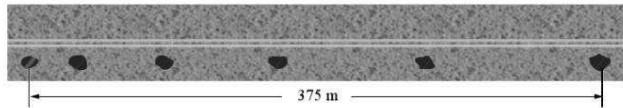
\includegraphics[width=0.5\linewidth]{../figs/VN10-2022-PH-TP004-1-P-1}
\end{center}
\begin{mcq}(4)
	\item $\SI{12.5}{\meter/\second}$.
	\item $\SI{15}{\meter/\second}$.
	\item $\SI{30}{\meter/\second}$.
	\item $\SI{25}{\meter/\second}$.
\end{mcq}
\hideall{
\textbf{Đáp án B.}\\
Tốc độ trung bình của ô tô:
$$v_\text{tb}=\dfrac{s}{t}=\dfrac{\SI{375}{\meter}}{\SI{25}{\second}}=\SI{15}{\meter/\second}.$$
}
	
	\item \mkstar{2}\\
	Một chiếc xe ô tô xuất phát từ A lúc 6 giờ sáng, chuyển động thẳng đều tới B, cách A $\SI{120}{\kilo\meter}$. Biết xe tới B lúc 8 giờ 30 phút sáng, tốc độ trung bình của xe là 
	\begin{mcq}(4)
		\item $\SI{48}{\kilo\meter/\hour}$.
		\item $\SI{45}{\kilo\meter/\hour}$.
		\item $\SI{60}{\kilo\meter/\hour}$.
		\item $\SI{50}{\kilo\meter/\second}$.
	\end{mcq}
\hideall{
	\textbf{Đáp án A.}\\
	Tốc độ trung bình của xe:
	$$v_\text{tb}=\dfrac{s}{t_2-t_1}=\SI{48}{\kilo\meter/\hour}.$$
}

	\item \mkstar{3}\\
	{Một xe chuyển động thẳng không đổi chiều, $\SI{1}{\hour}$ đầu xe chạy với tốc độ trung bình $\SI{60}{\kilo\meter/\hour}$ và $\SI{3}{\hour}$ sau xe chạy với tốc độ trung bình $\SI{40}{\kilo\meter/\hour}$. Tính tốc độ trung bình của xe trong suốt thời gian chuyển động.
		\begin{mcq}(4)
			\item $\SI{48}{\kilo\meter/\hour}$.
			\item $\SI{40}{\kilo\meter/\hour}$.
			\item $\SI{58}{\kilo\meter/\hour}$.
			\item $\SI{45}{\kilo\meter/\hour}$.
		\end{mcq}
	}
	\hideall{
		\textbf{Đáp án: D.}\\
		$$v_{tb}=\dfrac{v_1t_1+v_2t_2}{t_1+t_2}=\SI{45}{\kilo\meter/\hour}.$$
	}
	
	\item \mkstar{3}\\
	{Một người đi xe đạp trên $\dfrac{2}{3}$ đoạn đường đầu với tốc độ trung bình $\SI{10}{\kilo\meter/\hour}$ và $\dfrac{1}{3}$ đoạn đường sau với tốc độ trung bình $\SI{20}{\kilo\meter/\hour}$. Tốc độ trung bình của người đi xe đạp trên cả quãng đường là
		\begin{mcq}(4)
			\item $\SI{12}{\kilo\meter/\hour}$.
			\item $\SI{15}{\kilo\meter/\hour}$.
			\item $\SI{17}{\kilo\meter/\hour}$.
			\item $\SI{13.3}{\kilo\meter/\hour}$.
		\end{mcq}
	}
	\hideall{
		\textbf{Đáp án: A.}\\
		Gọi $s$ là chiều dài đoạn đường
		$$v_{tb}=\dfrac{s}{t_1+t_2}=\dfrac{s}{\dfrac{2s}{3v_1}+\dfrac{s}{3v_2}}=\dfrac{1}{\dfrac{2}{3v_1}+\dfrac{1}{3v_2}}=\SI{12}{\kilo\meter/\hour}.$$
	}
\end{enumerate}
\section{Bài tập tự luận}
\begin{enumerate}[label=\bfseries Bài \arabic*:,leftmargin=1.5cm]
	\item \mkstar{2}\\
	{		Hãy tính tốc độ trung bình ra m/s và km/h của nữ vận động viên tại một số giải thi đấu dựa vào bảng:
		\begin{center}
			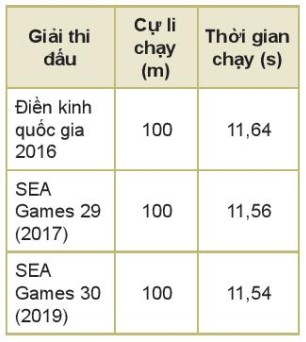
\includegraphics[width=0.3\linewidth]{../figs/VN10-2022-PH-TP005-5.jpg}
		\end{center}
	}
	\hideall
	{		Tốc độ trung bình của nữ vận động viên tại giải điền kinh quốc  gia 2016 là:
		$$v_\text{tb} = \dfrac{s}{t} =\dfrac{100}{\SI{11,64}{}} = \SI{8,6}{m/s} = \SI{30,96}{km/h}.$$
		Tốc độ trung bình của nữ vận động viên tại SEA GAME 19, 2017  là 100 : 
		$$v_\text{tb} = \dfrac{s}{t} =\dfrac{100}{\SI{11,56}{}} = \SI{8,65}{m/s} = \SI{31,141}{km/h}.$$
		Tốc độ trung bình của nữ vận động viên tại SEA GAME 30, 2019 là 100: 
		$$v_\text{tb} = \dfrac{s}{t} =\dfrac{100}{\SI{11,54}{}}= \SI{8,66}{m/s} = \SI{31,195}{km/h}.$$
	}

	\item \mkstar{2}
	
	
	{
		Một người đi xe máy đi từ ngã tư với tốc độ trung bình $\SI{30}{km/h}$ theo hướng Bắc. Sau 3 phút người đó đến vị trí nào trên hình?
		\begin{center}
			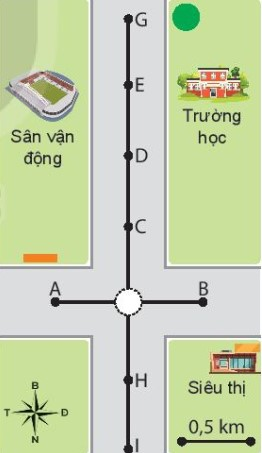
\includegraphics[width=0.25\linewidth]{../figs/VN10-2022-PH-TP005-1.jpg}
		\end{center}
	}
	\hideall
	{
		Sau 3 phút người đó đi được quãng đường là:
		
		$$s = vt = \SI{1,5}{km}.$$ 
		
		Như vậy người đó đến vị trí điểm E.
	}

	
	\item \mkstar{2}
	
	{
		
		Một ô tô chạy liên tục, trong 2 giờ đầu với tốc độ $\SI{80}{km/h}$, trong 1 giờ sau chạy với tốc độ $\SI{50}{km/h}$. Tốc độ trung bình của xe trong cả quá trình là bao nhiêu?
	}
	\hideall{
		
		Đoạn đường đi được trong 2 giờ đầu
		
		$$s_1 = v_1 t_1.$$
		
		Đoạn đường đi được trong 1 giờ sau
		
		$$s_2 = v_2t_2.$$
		
		Tốc độ trung bình của xe
		
		$$v_\text{tb} = \dfrac{s_1 + s_2}{t_1 + t_2} = \SI{70}{km/h}.$$
		
	}

\item \mkstar{2}

{
	
	Một người đi xe bắt đầu cho xe chạy trên đoạn đường thẳng: trong 10 giây đầu xe chạy được quãng đường $\SI{50}{m}$, trong 10 giây tiếp theo xe chạy được $\SI{150}{m}$. Tính tốc độ trung bình của xe máy trong khoảng thời gian nói trên.
}
\hideall{
	
	Tốc độ trung bình của xe máy
	
	$$v_\text{tb} = \dfrac{S_1 + S_2}{t_1 + t_2} = \SI{10}{m/s}.$$
}

	\item \mkstar{3}

{
	Một xe máy điện đi nửa đoạn đường đầu tiên với tốc độ trung bình $v_1 = \SI{24}{km/h}$ và nửa đoạn đường sau với tốc độ trung bình $v_2 = \SI{40}{km/h}$. Tính tốc độ trung bình trên cả đoạn đường.
	
}
\hideall{Gọi $2s$ là chiều dài cả đoạn đường.
	
	Thời gian đi nửa đoạn đường đầu:
	
	$$t_1 = \dfrac{s_1}{v_1} = \dfrac{s}{48}.$$
	
	Thời gian đi nửa đoạn đường cuối:
	
	$$t_2 = \dfrac{s_2}{v_2} = \dfrac{s}{80}.$$
	
	Tốc độ trung bình trên cả đoạn đường của xe máy điện:
	
	$$v = \dfrac{s}{t_1 + t_2} = \dfrac{s}{\dfrac{s}{48} + \dfrac{s}{80}} = \SI{30}{km/h}.$$
	
}

\item \mkstar{3}

{
	
	Một ô tô chạy trên đoạn đường thẳng từ A đến B phải mất khoảng thời gian $t$. Trong nửa đầu của khoảng thời gian này ô tô có tốc độ là $\SI{60}{km/h}$. Trong nửa khoảng thời gian cuối ô tô có tốc độ là $\SI{40}{km/h}$. Tính tốc độ trung bình trên cả đoạn AB.
}
\hideall{
	
	Tốc độ trung bình:
	
	$$v_\text{tb} = \dfrac{S}{t} = \dfrac{v_1\cdot\dfrac{t}{2}+v_2\cdot\dfrac{t}{2}}{t}=\dfrac{v_1 + v_2}{2} =\SI{50}{km/h}.$$		
}



\item \mkstar{3}

{
	
	Một người đi xe đạp từ A đến B với tốc độ $\SI{12}{km/h}$ trong $\dfrac{1}{3}$ quãng đường, và tốc độ $\SI{18}{km/h}$ trong $\dfrac{2}{3}$ quãng đường còn lại. Tính tốc độ trung bình của người đó trên cả đoạn đường AB.
}
\hideall{
	
	Thời gian đi $\dfrac{1}{3}$ quãng đường đầu:
	
	$$t_1 = \dfrac{S}{3v_1} = \dfrac{S}{36}.$$
	
	Thời gian đi $\dfrac{2}{3}$ quãng đường còn lại:
	
	$$t_2 = \dfrac{2S}{3v_2} = \dfrac{S}{27}.$$
	
	Tốc độ trung bình của người đó
	
	$$v_\text{tb} = \dfrac{S}{t_1 + t_2} = \dfrac{S}{\dfrac{S}{36} + \dfrac{S}{27}} \approx \SI{15,43}{km/h}.$$
}

\item \mkstar{3}

{
	
	Một chiếc thuyền cao tốc đi từ bến A đến bến B. Trong $\dfrac{2}{3}$ thời gian đầu tốc độ của thuyền là $v_1 = \SI{45}{km/h}$, thời gian còn lại thuyền chuyển động với tốc độ $v_2$ bằng bao nhiêu để tốc độ trung bình của nó trên cả quãng đường AB là $v = \SI{48}{km/h}$?
	
}
\hideall{
	
	Tốc độ trung bình của thuyền trên đoạn đường AB:
	$$v_\text{tb}=\dfrac{v_1\cdot\dfrac{2t}{3}+v_2\cdot\dfrac{t}{3}}{t}=\dfrac{2v_1}{3}+\dfrac{v_2}{3}\Rightarrow v_2=\SI{54}{\kilo\meter/\hour}.$$
}

\item \mkstar{3}\\
{	Một người đua xe đạp đi trên $\dfrac{1}{3}$ quãng đường đầu với tốc độ $\SI{25}{km/h}$. Tính tốc độ của người đó đi trên đoạn đường còn lại. Biết rằng tốc độ trung bình trên cả đoạn đường là $v_\text{tb} = \SI{20}{km/h}$.
}
\hideall{
	Tốc độ trung bình trên cả đoạn đường
	$$v_\text{tb}=\dfrac{s}{\dfrac{s}{3v_1}+\dfrac{2s}{3v_2}}=\dfrac{1}{\dfrac{1}{3v_1}+\dfrac{2}{3v_2}}$$
	$$\Leftrightarrow 20=\dfrac{1}{\dfrac{1}{3\cdot25}+\dfrac{2}{3v_2}}\Rightarrow v_2=\SI{18.18}{\kilo\meter/\hour}.$$
}




	\item \mkstar{3}\\
	{Một ô tô đi trên quãng đường AB với tốc độ trung bình $\SI{54}{km/h}$. Nếu giảm tốc độ trung bình đi $\SI{9}{km/h}$ thì ôtô đến B trễ hơn dự định 45 phút. Tính quãng đường AB và thời gian dự tính để đi quãng đường đó.
	}
	\hideall{Gọi $t$ là thời gian dự định để đi quãng đường AB, $v$ là tốc độ trung bình ban đầu và $s$ là chiều dài quãng đường AB. Phương trình chuyển động cho các trường hợp đi đúng tốc độ trung bình dự kiến và đi chậm hơn lần lượt là 
		\begin{equation}
			\label{eq:1}
			s=vt=54t
		\end{equation}
	\begin{equation}
		\label{eq:2}
		s=\left(v-9\right)\left(t+\SI{0.75}{}\right)=45\left(t+\SI{0.75}{}\right)
	\end{equation}
		Từ phương trình (\ref{eq:1}) và phương trình (\ref{eq:2}), giải được $t=\SI{3,75}{\hour}$.	\\
		Chiều dài quãng đường AB: $s=54t=\SI{202.5}{\kilo\meter}$.
		
	}

\item \mkstar{3}

{
	Một cậu bé dắt chó đi dạo về nhà, khi còn cách nhà $\SI{10}{m}$, con chó chạy về nhà với tốc độ $\SI{5}{m/s}$. Vừa đến nhà nó lại chạy ngay lại với tốc độ $\SI{3}{m/s}$. Tính tốc độ trung bình của chú chó trong quãng đường đi được kể từ lúc chạy về nhà đến lúc gặp lại cậu bé, biết cậu bé đi đều với tốc độ $\SI{1}{m/s}$.
}
\hideall{
	
	Thời gian chú chó về đến nhà là
	
	$$t_1 = \dfrac{s_1}{v_c} = \SI{2}{s}.$$
	
	Trong thời gian đó cậu bé đi được
	
	$$s_n = t_1 v_n = 1 \cdot 2 = \SI{2}{m}.$$
	
	Khoảng cách từ cậu bé đến nhà lúc đó là
	
	$$s' = s - s_n = \SI{8}{m}.$$
	
	Thời gian chú chó chạy từ nhà tới lúc gặp lại cậu bé
	
	$$t_2 = \dfrac{s'}{v_c + v_n} = \SI{2}{s}.$$
	
	Chú chó đã quay lại một đoạn là:
	
	$$s_2 = v_ct_2 = 3 \cdot 2 = \SI{6}{m}.$$
	
	
	Tốc độ trung bình của chú chó trong cả quá trình là: 
	
	$$v_\text{tb} = \dfrac{s_1 + s_2}{t_1 + t_2} = \SI{4}{m/s}.$$
}

	
	\item \mkstar{3}
	
	{
		
		Một người đi xe máy chuyển động trên đường thẳng theo 3 giai đoạn: Giai đoạn 1 chuyển động với tốc độ không đổi $v_1 = \SI{30}{km/h}$ trong $\SI{10}{km}$ đầu tiên; giai đoạn 2 chuyển động với tốc độ $v_2 = \SI{40}{km/h}$ trong 30 phút; giai đoạn 3 chuyển động trên đoạn đường $\SI{4}{km}$ trong 10 phút. Tính tốc độ trung bình trên cả đoạn đường.
	}
	\hideall{
		
		Thời gian xe máy chuyển động giai đoạn đầu
		
		$$t_1 = \dfrac{s_1}{v_1} = \dfrac{1}{3}\ \text{h}.$$
		
		Quãng đường giai đoạn sau:
		
		$$s_2 = v_2t_2 = \SI{20}{km}.$$
		
		Ta có:
		
		$$s = s_1 + s_2 + s_3 = \SI{34}{km}.$$
		
		$$t = t_1 + t_2 + t_3 = \SI{1}{h}.$$
		
		Tốc độ trung bình của xe máy trên cả đoạn đường:
		
		$$v_\text{tb} = \dfrac{s}{t} = \SI{34}{km/h}.$$
		
	}

	

	\item \mkstar{3}
	
	{
		Một ô tô chuyển động trên đoạn đường MN. Trong một phần hai quãng đường đầu đi với $v = \SI{40}{km/h}$. Trong một phần hai quãng đường còn lại đi trong một phần hai thời gian đầu với $v = \SI{75}{km/h}$ và trong một phần hai thời gian cuối đi với $v = \SI{45}{km/h}$. Tính tốc độ trung bình trên đoạn MN.
	}
	\hideall{
		
		Tốc độ trung bình trong nữa quãng đường cuối:
		$$v_\text{tb 2}=\dfrac{v_2\cdot\dfrac{t}{2}+v_3\cdot \dfrac{t}{2}}{t}=\dfrac{v_2+v_3}{2}=\SI{60}{\kilo\meter/\hour}$$
		Tốc độ trung bình trên cả đoạn đường:
		$$v_\text{tb}=\dfrac{s}{\dfrac{s}{2v_1}+\dfrac{s}{2v_\text{tb 2}}}=\dfrac{2}{\dfrac{1}{v_1}+\dfrac{1}{v_\text{tb 2}}}=\SI{48}{\kilo\meter/\hour}.$$
	}
	
	\item \mkstar{3}
	
	{
		
		Một người đi xe máy trên một đoạn đường thẳng AB. Trên một phần ba đoạn đường đầu đi với $v_1 = \SI{30}{km/h}$, một phần ba đoạn đường tiếp theo với $v_2 = \SI{36}{km/h}$ và một phần ba đoạn đường cuối cùng đi với $v_3= \SI{48}{km/h}$. Tính $v_\text{tb}$ trên cả đoạn AB.
		
	}
	\hideall{
		
	Tốc độ trung bình trên của đoạn đường AB:
	$$v_\text{tb}=\dfrac{s}{\dfrac{s}{3v_1}+\dfrac{s}{3v_2}+\dfrac{s}{3v_3}}=\dfrac{3}{\dfrac{1}{v_1}+\dfrac{1}{v_2}+\dfrac{1}{v_3}}=\SI{36.61}{\kilo\meter/\hour}.$$
	}
\end{enumerate}
%				\let\lesson\undefined
\newcommand{\lesson}{\phantomlesson{Bài 4: Chuyển động thẳng}}
\chapter[Vận tốc và đồ thị độ dịch chuyển - thời gian]{Vận tốc và đồ thị độ dịch chuyển - thời gian}
\setcounter{section}{0}
\section{Lý thuyết}
\subsection{Vận tốc}
\subsubsection{Vận tốc trung bình}
Vận tốc trung bình là đại lượng vectơ được xác định bằng thương số giữa độ dịch chuyển của vật và thời gian để vật thực hiện độ dịch chuyển đó
$$\overrightarrow{v_\text{tb}}=\dfrac{\vec{d}}{\Delta t}=\dfrac{\Delta \vec{x}}{\Delta t}$$
\luuy{Tốc độ trung bình chỉ bằng độ lớn của vận tốc trung bình khi vật chuyển động thẳng không đổi chiều.}
\subsection{Phương trình chuyển động thẳng đều}
Xét một chất điểm chuyển động thẳng đều trên đường thẳng O$x$ với tốc độ $v$. Ở thời điểm ban đầu ($t_0=0$), vật ở vị trí A cách gốc O một đoạn $x_0$. Vào thời điểm $t$, vật ở vị trí M cách gốc O một đoạn $x$.  
\begin{center}
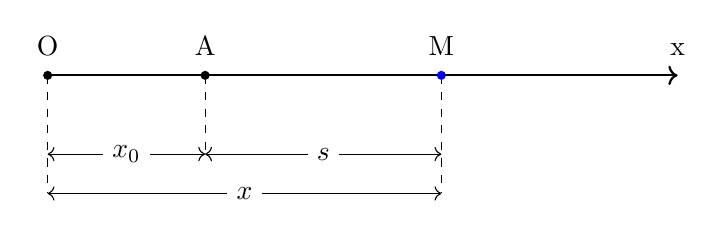
\begin{tikzpicture}
	\coordinate (O) at (0,0);
	\coordinate (A) at (2,0);
	\coordinate (M) at (5,0);
	\coordinate (x) at (8,0);
	\coordinate (O1) at ($(O)-(0,1cm)$);
	\coordinate (A1) at ($(A)-(0,1cm)$);
	\draw[->,thick] (O) -- (x);
	\foreach \i in {O,A}{
		\filldraw[black] (\i) circle (0.5mm);
	}
	\node[label=90:O] at (O){};	
	\node[label=90:A] at (A){};
	\node[label=90:M] at (M){};	
	\node[label=90:x] at (x){};	
	\draw[<->] (O1) -- (A1);
	\node [fill=white] (F1) at ($(O1)!0.5!(A1)$) {$x_0$};
	\coordinate (M1) at ($(M)-(0,1cm)$);
	\draw[<->] (A1) -- (M1);
	\node [fill=white] (F2) at ($(A1)!0.5!(M1)$) {$s$};
	\coordinate (O2) at ($(O)-(0,1.5cm)$);
	\coordinate (M2) at ($(M)-(0,1.5cm)$);
	\draw[<->] (O2) -- (M2);
	\node [fill=white] (F3) at ($(O2)!0.5!(M2)$) {$x$};
	\draw[dashed] (O) -- (O2);
	\draw[dashed] (A) -- (A1);
	\draw[dashed] (M) -- (M2);
	\filldraw[blue] (M) circle (0.5mm);
	%		\node[above of=O]()
\end{tikzpicture}
\end{center}

Tọa độ của chất điểm sau thời gian chuyển động $t$ là:
\begin{equation}
x=x_0+s=x_0+vt.
\end{equation}
Phương trình dùng để xác định tọa độ của M theo thời gian được gọi là phương trình chuyển động của chất điểm M. Trong trường hợp này, M chuyển động thẳng đều nên phương trình này gọi là phương trình chuyển động thẳng đều của điểm M. 
\subsection{Đồ thị độ dịch chuyển - thời gian}
Đồ thị độ dịch chuyển - thời gian của hai vật A và B được mô tả như hình \ref{fig:5.1}
\begin{center}
	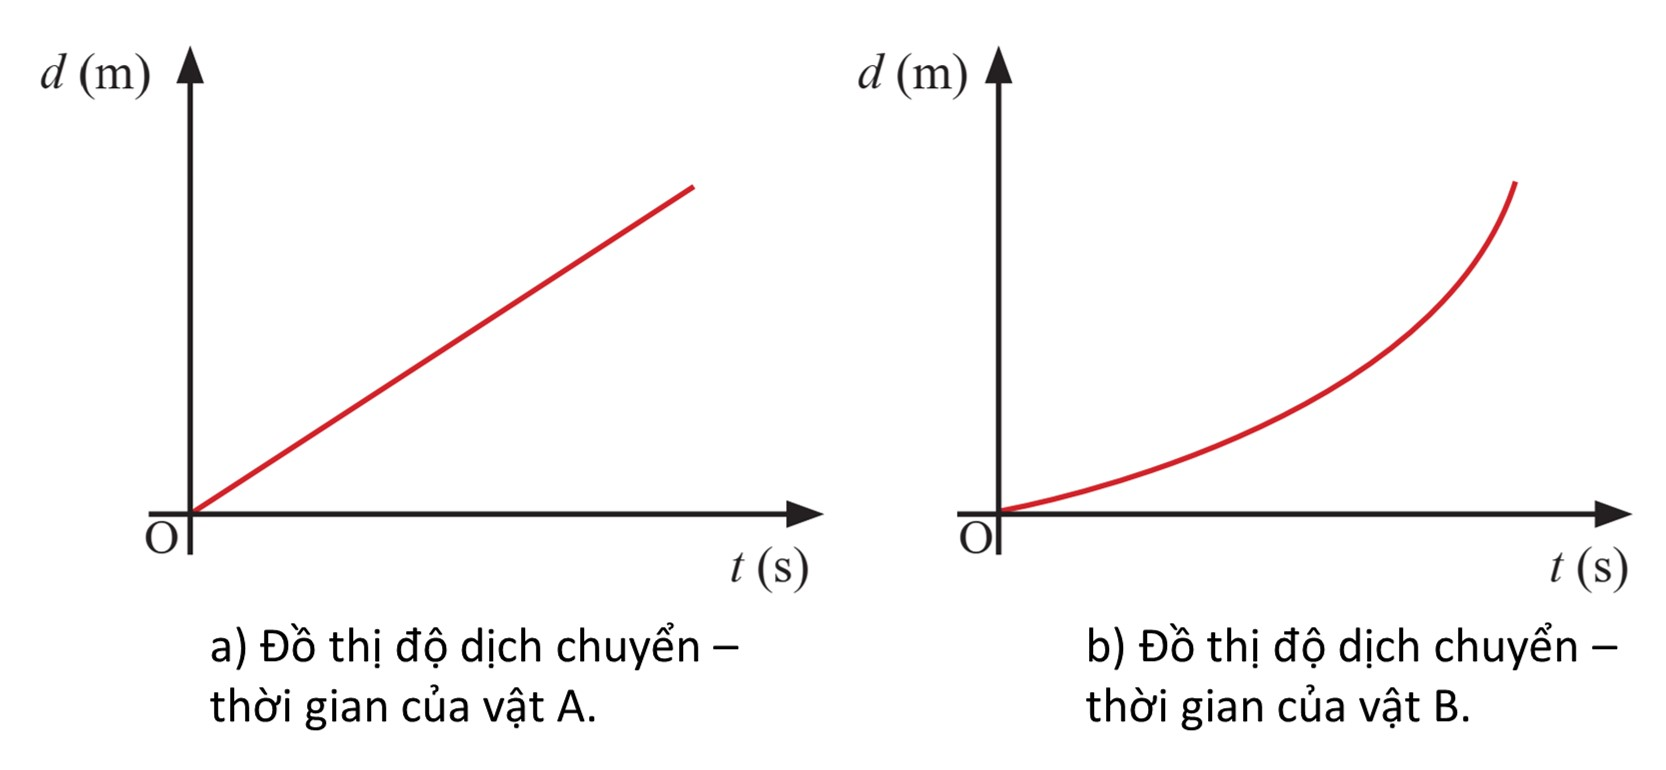
\includegraphics[width=0.6\linewidth]{../figs/VN10-2023-PH-TP005-1}
	\captionof{figure}{}
	\label{fig:5.1}
\end{center}
Từ các đồ thị $\left(d-t\right)$, ta có nhận xét:
\begin{enumerate}[label=\alph*)]
	\item Đồ thị $\left(d-t\right)$ mô tả chuyển động của vật $A$ là đường thẳng đi qua gốc toạ độ. Chuyển động của vật $A$ là chuyển động thẳng đều.
	\item Đồ thị $\left(d-t\right)$ mô tả chuyển động của vật $B$ là đường cong qua gốc toạ độ. Độ dịch chuyển của vật B trong những khoảng thời gian bằng nhau tăng lên nên chuyển động của vật B là chuyển động thẳng nhanh dần.
\end{enumerate}
\subsubsection{Xác định vận tốc từ độ dốc của đồ thị $\left(d-t\right)$}
\textbf{Xác định vận tốc trung bình từ đồ thị độ dịch chuyển - thời gian}\\
Xét vật chuyển động từ vị trí 1 (tại thời điểm $t_1$) đến vị trí 2 (tại thời điểm $t_2$) lần lượt được biểu diễn bởi hai điểm $P$ và $Q$ trên đồ thị ($d$ – $t$) trong hình \ref{fig:5.2}. So sánh với biểu thức để xác định vận tốc trung bình, ta có: độ dịch chuyển $d$ của vật chính là đoạn $HQ$, khoảng thời gian $\Delta t$ chính là độ dài $PH$.\\
\begin{center}
	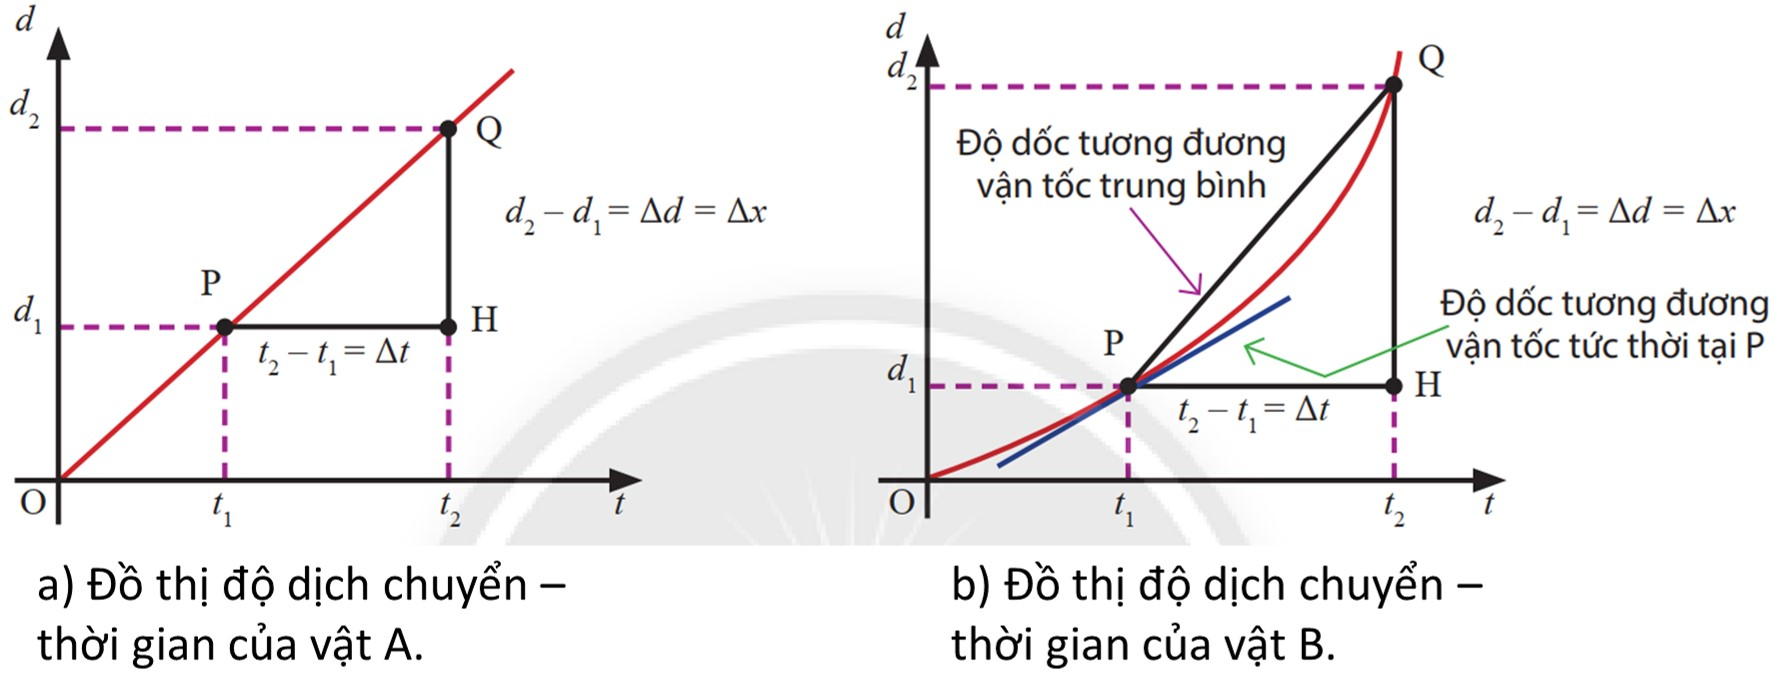
\includegraphics[width=0.8\linewidth]{../figs/VN10-2023-PH-TP005-2}
	\captionof{figure}{}
	\label{fig:5.2}
\end{center}
Từ đó, ta thấy vận tốc trung bình chính là độ dốc của đoạn $PQ$ nối hai điểm trên đồ thị biểu diễn vị trí đầu đến vị trí cuối của vật.\\
\textbf{Xác định vận tốc tức thời từ đồ thị độ dịch chuyển - thời gian}\\
Vận tốc tức thời của vật tại một thời điểm được xác định bởi độ dốc của tiếp tuyến với đồ thị ($d$ - $t$) tại thời điểm đang xét.\\
Tốc độ tức thời tại một thời điểm chính là độ lớn của độ dốc tiếp tuyến của đồ thị ($d$ - $t$) tại điểm đó.
\section{Mục tiêu bài học - Ví dụ minh họa}
\begin{dang}{Nhận biết được phương trình chuyển động thẳng đều}
	\viduii{2}{ Trong các phương trình chuyển động thẳng đều sau đây, phương trình nào biểu diễn chuyển động không xuất phát từ gốc tọa độ và ban đầu hướng về gốc tọa độ:
		\begin{mcq}(2)
			\item $x = 80 - 30t.$
			\item $x = 15 + 40t.$
			\item $x = -6t.$
			\item $x = -10 - 6t.$
		\end{mcq}
	}
	{\hide{
		Phương trình chuyển động của vật là 
		$$x=x_0 +vt.$$	
		Chuyển động không xuất phát từ gốc tọa độ thì $x_0 \neq  0$.
		
		Ban đầu vật hướng về gốc tọa độ thì vị trí ban đầu và vận tốc của vật phải thỏa mãn 
		\begin{equation*}
			\left\lbrace
			\begin{array}{rl}
				x_0&<0,\\
				v&>0
			\end{array}
			\right.
			\qquad\text{hoặc}\qquad
			\left\lbrace
			\begin{array}{rl}
				x_0&>0,\\
				v&<0
			\end{array}
			\right.
		\end{equation*}
		Hình vẽ sau minh họa hai trường hợp này.
		\begin{center}
			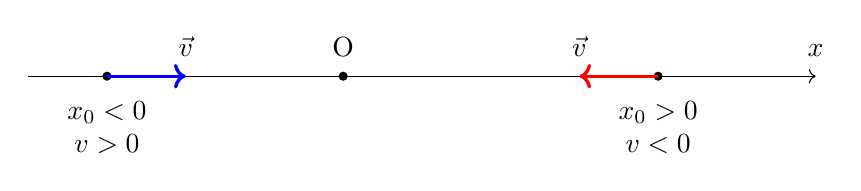
\begin{tikzpicture}
				\coordinate (O) at (0,0);
				\coordinate (A) at (-3,0);
				\coordinate (A1) at ($(A)+(1,0)$);
				\coordinate (M) at (4,0);
				\coordinate (M1) at ($(M)-(1,0)$);
				\coordinate (x) at (6,0);
				\coordinate (X) at (-4,0);
				\draw[->] (X) -- (x);
				\foreach \i in {O,A,M}{
					\filldraw[black] (\i) circle (0.5mm);
				}
				\draw[->,very thick,blue] (A) -- (A1);
				\draw[->,very thick,red] (M) -- (M1);
				\node[label=90:O] at (O){};	
				\node[label=90:$\vec{v}$]at (A1){};
				\node[label=90:$\vec{v}$]at (M1){};
				\node[align=center,below=0.2cm of A](Mnode){$x_0<0$\\$v>0$};
				\node[align=center,below=0.2cm of M](Mnode){$x_0>0$\\$v<0$};
				\node[label=90:$x$]at (x){};
			\end{tikzpicture}
		\end{center}
		Trong các lựa chọn, chỉ có lựa chọn A ($x = 80 - 30t$) thỏa mãn với điều kiện trên.
		
		\textbf{Đáp án: A}.
	}}
\end{dang}

\begin{dang}{Xây dựng phương trình, tính các đại lượng\\ trong phương trình chuyển động thẳng đều\\ cho một hoặc hai vật.}
	\viduii{2}{Một vật chuyển động thẳng đều với tốc độ $\SI{2}{m/s}$. Lúc $t = \SI{2}{s}$ vật có tọa độ $\SI{5}{m}$. Phương trình chuyển động của vật là 
		\begin{mcq}(2)
			\item $x=2t+1\qquad\left(\si{\meter}, \si{\second}\right)$.
			\item $x=-2t +5\qquad\left(\si{\meter}, \si{\second}\right)$.
			\item $x=2t+5\qquad\left(\si{\meter}, \si{\second}\right)$.
			\item $x=-2t+1\qquad\left(\si{\meter}, \si{\second}\right)$.
		\end{mcq}
	}
	{\hide{
		Phương trình tọa độ của vật có dạng: 
		$$x=x_0 +vt.$$
		
		Thay $x=\SI{5}{m}$, $v=\SI{2}{m/s}$, $t=\SI{2}{s}$ vào ta suy ra 
		\begin{align*}
			x_0=x-vt=\SI{5}{m}-\SI{2}{\meter/\second}\cdot\SI{2}{s}=\SI{1}{m}.
		\end{align*}
		
		Vậy phương trình chuyển động của vật là:
		
		$$x=1+2t =2t+1\qquad\left(\si{\meter}, \si{\second}\right).$$
		
		\textbf{Đáp án: A}.
	}}

	\viduii{3}{	Trên đường thẳng từ nhà đến chỗ làm việc của A, cùng một lúc xe 1 khởi hành từ nhà đến chỗ làm với $v_1=\SI{80}{\km/\hour}$. Xe 2 từ chỗ làm đi cùng chiều xe 1 với $v_2=\SI{60}{\km/\hour}$. Biết quãng đường từ nhà đến chỗ làm là $\SI{40}{\km}$. Lập phương trình chuyển động của mỗi xe với cùng hệ quy chiếu.
	}
	{\hide{
		Chọn hệ quy chiếu gồm:
		\begin{itemize}
			\item Chiều dương cùng chiều với chiều chuyển động với hai xe;
			\item Gốc tọa độ tại A;
			\item Mốc thời gian lúc hai xe bắt đầu xuất phát.
		\end{itemize}
		
		Xe 1 có phương trình chuyển động
		\begin{equation*}
			x_1=x_0 + v_1t = 80t\textrm{ (km, h)}.
		\end{equation*}
		Xe 2 có phương trình chuyển động  
		\begin{equation*}
			x_2=x_0 + v_2t = 40+60t\textrm{ (km, h)}.
		\end{equation*}
	}}


	\viduii{3}{	Hai vật chuyển động ngược chiều qua A và B cùng một lúc. Vật qua A có tốc độ $v_1=\SI{10}{\meter/\second}$, vật qua B có tốc độ $v_2=\SI{15}{\meter/\second}$. Cho biết AB có chiều dài $\SI{100}{m}$. Lấy trục tọa độ là đường thẳng AB, gốc tọa độ ở B, chiều dương từ A sang B, mốc thời gian là lúc chúng cùng qua A và B. Lập phương trình chuyển động của mỗi vật.
	}
	{\hide{
		Hệ quy chiếu gồm:
		\begin{itemize}
			\item Gốc tọa độ tại B;
			\item Chiều dương từ A sang B;
			\item Mốc thời gian lúc hai vật cùng qua A và B.
		\end{itemize}
		
		Phương trình chuyển động của vật qua A là
		\begin{equation*}
			x_\text{A}=x_{0\text{A}} + v_\text{A}t =-100+10t\textrm{ (m, s)}.
		\end{equation*}
		
		Phương trình chuyển động của vật qua B là
		\begin{equation*}
			x_\text{B}=x_{0\text{B}} + v_\text{B}t = -15t\textrm{ (m, s)}.
		\end{equation*}
		
	}}
\end{dang}

\begin{dang}{Xác định vị trí, thời điểm \\hai vật chuyển động thẳng đều gặp nhau}
\viduii{3}{	Hai vật chuyển động ngược chiều qua A và B cùng một lúc. Vật qua A có tốc độ $v_1=\SI{10}{\meter/\second}$, vật qua B có tốc độ $v_2=\SI{15}{\meter/\second}$. Cho biết AB có chiều dài $\SI{100}{m}$. Xác định vị trí và thời điểm chúng gặp nhau.
	
}
{\hide{
	Chọn gốc tọa độ ở vị trí A, gốc thời gian ở thời điểm hai vật đang ở A và B. Chiều dương trục toạ độ hướng từ A sang B.\\
	Phương trình chuyển động của hai vật:
	\begin{equation*}
		\begin{cases}
			x_1=x_{01}+v_1t\\
			x_2=x_{02}+v_2t
		\end{cases}
	\Rightarrow
	\begin{cases}
		x_1=10t\\
		x_2=100-15t
	\end{cases}
\left(\si{\meter}, \si{\second}\right)
	\end{equation*}
	Hai vật gặp nhau khi chúng có cùng tọa độ
	\begin{equation*}
		x_\text{1}=x_\text{2}\Rightarrow 10t=100-15t \Rightarrow t=\SI{4}{\second}.
	\end{equation*}
	Dựa vào phương trình chuyển động, ta xác định được vị trí hai vật gặp nhau 
	\begin{equation*}
		x_\text{1}=x_\text{2}=10t=\SI{40}{\meter}.
	\end{equation*}
}}

\viduii{3}{Lúc 7 giờ, một người ở A chuyển động thẳng đều với tốc độ $ v_A= \SI{36}{km/h}$ đuổi theo người ở B đang chuyển động với tốc độ $v_B = \SI{5}{m/s}$. Biết $AB = \SI{18}{km}$. Hai người đuổi kịp nhau tại nơi cách A một khoảng 
	\begin{mcq}(4)
		\item $\SI{58}{km}$.
		\item $\SI{46}{km}$.
		\item $\SI{36}{km}$.
		\item $\SI{24}{km}$.
	\end{mcq}
}
{\hide{
	$v_B = \SI{5}{m/s}=\SI{18}{\kilo\meter/\hour}$\\
	Chọn gốc toạ độ tại A, chiều dương trục toạ độ hướng từ A đến B, gốc thời gian lúc 7 giờ.\\
	Phương trình chuyển động của hai người ở A và B:
	\begin{equation*}
		\begin{cases}
			x_\text{A}=36t\\
			x_\text{B}=18+18t
		\end{cases}
	\left(\si{\meter}, \si{\second}\right)
	\end{equation*}
	Khi hai người gặp nhau, tọa độ của hai người trùng nhau  
	\begin{align*}
		x_1&=x_2 \quad
		\Rightarrow\quad 36t=18+18t\quad\Rightarrow\quad t=\SI{1}{h}
	\end{align*}
	Dựa vào phương trình chuyển động, suy ra nơi gặp nhau cách A
	$$x_\text{A}  =36t=\SI{36}{\kilo\meter/\hour}\cdot\SI{1}{\hour}= \SI{36}{km}.$$
	
	
	\textbf{Đáp án: C}.
}}
\end{dang}

\begin{dang}{Thực hiện xác định quãng đường, vận tốc và thời gian dựa vào phương trình chuyển động thẳng đều}
	\viduii{3}{Xe thứ nhất đi từ A đến B mất 8 giờ, xe thứ hai đi từ B đến A mất 6 giờ. Nếu hai xe khởi hành cùng một lúc từ A và B để đến gần nhau thì sau 3 giờ hai xe cách nhau $\SI{30}{km}$. Tính chiều dài của quãng đường AB.
	}
	{\hide{
		Gọi $v_1$; $v_2$ lần lượt là tốc độ của xe thứ nhất và xe thứ hai. Từ quãng đường AB và thời gian chuyển động, ta tính được tỉ số tốc độ của hai xe
		\begin{align*}
			v_1&=\dfrac{s}{t_1},\\
			v_2&=\dfrac{s}{t_2},\\
			\Rightarrow \dfrac{v_1}{v_2}&=\dfrac{t_2}{t_1}=\dfrac{\SI{6}{\hour}}{\SI{8}{\hour}}=\dfrac{3}{4}\\
			\Rightarrow v_1&=\dfrac{3}{4} v_2.
		\end{align*}
		
		Nếu chọn gốc tọa độ tại vị trí A, chiều dương từ A đến B và gốc thời gian là lúc 2 xe xuất phát thì phương trình chuyển động của mỗi xe:
		\begin{align*}
			x_1 &=v_1t=\dfrac{3}{4}v_2 t,\\
			x_2&=s-v_2t=v_2t_2-v_2t.
		\end{align*}
		
		Sau 3 giờ: $$|x_1-x_2|=\SI{30}{km} \Rightarrow v_2=\SI{40}{km/h}.$$
		
		Chiều dài của quãng đường AB: $$s=v_2t_2=\SI{40}{\kilo\meter/\hour}\cdot\SI{6}{\hour} =\SI{240}{km}.$$
		
	}}
	
\viduii{3}{Hai vật chuyển động ngược chiều qua A và B cùng một lúc. Vật qua A có tốc độ $v_1=\SI{10}{\meter/\second}$, vật qua B có tốc độ $v_2=\SI{15}{\meter/\second}$. Cho biết AB có chiều dài $\SI{100}{m}$. Xác định vị trí và thời điểm chúng cách nhau $\SI{25}{\meter}$.
}
{\hide{
	Chọn gốc tọa độ ở A, chiều dương trục toạ độ hướng từ A đến B và gốc thời gian là thời điểm hai vật đang đi qua A và B. Gọi $s=\SI{100}{\meter}$ là chiều dài đoạn AB. Phương trình chuyển động của hai vật lần lượt là 
	\begin{equation}
		\begin{cases}
			x_1&=v_1t\\
			x_2&=s-v_2t
		\end{cases}
	\Rightarrow \begin{cases}
		x_1=10t\\
		x_2=100-15t
	\end{cases}
\left(\si{\meter}, \si{\second}\right)
	\end{equation}	
	Khi hai vật cách nhau $d=\SI{25}{\meter}$
	\begin{equation*}
		d=\left|x_\text{A}-x_\text{B}\right|=\SI{25}{\meter}.
	\end{equation*}
	\begin{align*}
	\Leftrightarrow	\left|10t-100+15t\right|=25\Rightarrow t=\SI{3}{\second} \vee t=\SI{5}{\second}.
	\end{align*}
\begin{itemize}
	\item 	Với $t=\SI{3}{\second}$, thay vào phương trình chuyển động, ta được vị trí hai vật
	\begin{align*}
		\begin{cases}
			x_\text{1}=v_1t=\left(\SI{10}{\meter/\second}\right)\cdot\left(\SI{3}{\second}\right)=\SI{30}{\meter}\\
			x_\text{2}=s-v_2t=\SI{100}{\meter}-\left(\SI{15}{\meter/\second}\right)\cdot\left(\SI{3}{\second}\right)=\SI{55}{\meter}.
		\end{cases}
	\end{align*}
\item Với $t=\SI{5}{\second}$, thay vào phương trình chuyển động, ta được vị trí hai vật 
\begin{align*}
	\begin{cases}
		x_\text{1}=v_1t=\left(\SI{10}{\meter/\second}\right)\cdot\left(\SI{5}{\second}\right)=\SI{50}{\meter}\\
		x_\text{2}=s-v_2t=\SI{100}{\meter}-\left(\SI{15}{\meter/\second}\right)\cdot\left(\SI{5}{\second}\right)=\SI{25}{\meter}.
	\end{cases}
\end{align*}
\end{itemize}
}}

\end{dang}
\begin{dang}{Tính được tốc độ từ độ dốc của đồ thị độ dịch chuyển – thời gian.}
	\viduii{2}
	{Một vật chuyển động có đồ thị ($d$-$t$) được mô tả như hình \ref{fig:5.3}. Hãy xác định tốc độ tức thời của vật tại các vị trí $A, B$ và $C$.
		\begin{center}
			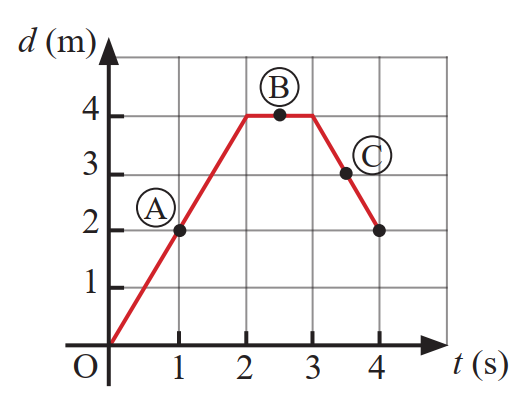
\includegraphics[width=0.35\linewidth]{../figs/VN10-2023-PH-TP005-3}
			\captionof{figure}{}
			\label{fig:5.3}
		\end{center}
	}
	{\hide{
		Tốc độ tức thời tại một thời điểm chính là độ dốc của tiếp tuyến với đồ thị ($d$ - $t$) tại điểm đó:
	\begin{itemize}
		\item Tốc độ tức thời tại $A$
		$$v_A=\dfrac{\left|2-0\right|}{1-0}=\SI{2}{\meter/\second}$$
		\item Tốc độ tức thời tại điểm $B$
		$$v_B=\dfrac{\left|4-4\right|}{3-2}=\SI{0}{\meter/\second}$$
		\item Tốc độ tức thời tại điểm $C$
		$$v_C=\dfrac{\left|2-4\right|}{4-3}=\SI{2}{\meter/\second}$$
	\end{itemize}
	}}

\viduii{3}
{Đồ thị độ dịch chuyển – thời gian trong chuyển động thẳng của một xe ô tô đồ chơi điều khiển từ xa được vẽ ở hình \ref{fig:5.4}.
	\begin{center}
		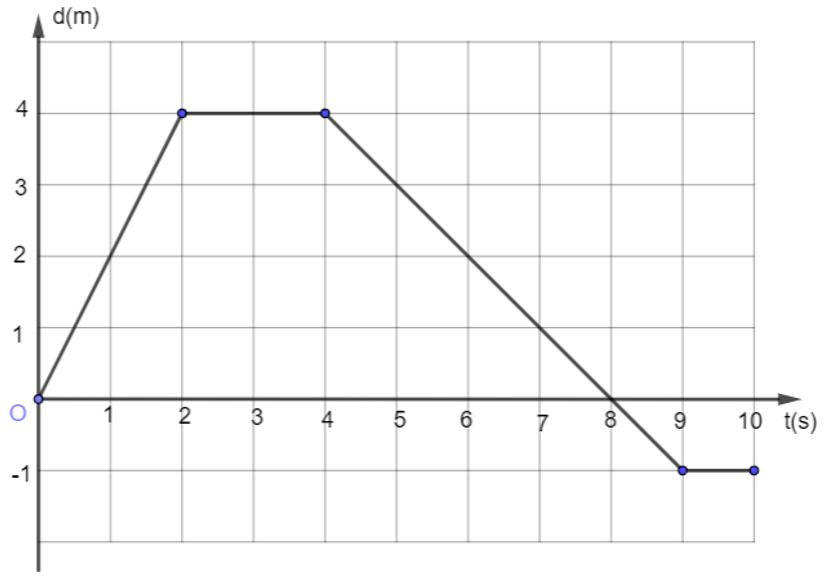
\includegraphics[width=0.5\linewidth]{../figs/VN10-2023-PH-TP005-4}
		\captionof{figure}{}
		\label{fig:5.4}
	\end{center}
	\begin{enumerate}[label=\alph*)]
		\item Mô tả chuyển động của xe.
		\item Xác định vị trí của xe so với điểm xuất phát của xe ở giây thứ 2, giây thứ 4, giây thứ 8 và giây thứ 10.
		\item Xác định tốc độ và vận tốc của xe trong 2 giây đầu, từ giây 2 đến giây 4 và từ giây 4 đến giây 8.
		\item Xác định quãng đường đi được và độ dịch chuyển của xe sau 10 giây chuyển động. Tại sao giá trị của chúng không giống nhau?
	\end{enumerate}
	
}
{\hide{
\begin{enumerate}[label=\alph*)]
	\item \begin{itemize}
		\item Trong 2 giây đầu xe chuyển động với vận tốc không đổi.
		\item Từ giây 2 đến giây 4 xe dừng lại.
		\item Từ giây 4 đến giây 8 xe đổi chiều chuyển động theo hướng ngược lại với vận tốc nhỏ hơn lúc đi và quay lại vị trí xuất phát.
		\item Từ giây 8 đến giây 9 xe đi tiếp với vận tốc đó thêm 1 đoạn rồi mới dừng lại.
		\item Từ giây 9 đến giây 10 xe dừng lại.
	\end{itemize}
	\item \begin{itemize}
		\item Ở giây thứ 2: xe cách vị trí xuất phát $\SI{4}{\meter}$.
		\item Ở giây thứ 4: xe vẫn cách vị trí xuất phát $\SI{4}{\meter}$.
		\item Ở giây thứ 8: xe quay lại vị trí xuất phát.
		\item Ở giây thứ 10: xe ở sau vị trí xuất phát $\SI{1}{\meter}$.
	\end{itemize}
	\item \begin{itemize}
		\item Trong 2 giây đầu: vận tốc của xe = tốc độ của xe $=\dfrac{\left|4-0\right|}{2-1}=\SI{2}{\meter/\second}$.
		\item Từ giây 4 đến giây 8
		\begin{itemize}
			\item tốc độ của xe $=\dfrac{\left|0-4\right|}{8-4}=\SI{1}{\meter/\second}$.
			\item vận tốc của xe $=\dfrac{0-4}{8-4}=\SI{-1}{\meter/\second}$.
		\end{itemize}
	\end{itemize}
	\item Sau 10 giây chuyển động thì 
	\begin{itemize}
		\item quãng đường xe đi được là $s=4+0+4+1=\SI{9}{\meter}$.
		\item độ dịch chuyển: $d=\SI{-1}{\meter}$.
	\end{itemize}
	Khi vật chuyển động thẳng, có đổi chiều thì quãng đường đi được và độ dịch chuyển có độ lớn không bằng nhau.
\end{enumerate}
}}
\end{dang}
\begin{dang}{Xây dựng đồ thị tọa độ - thời gian,\\ chọn tỉ xích, lập bảng giá trị tương ứng \\cho một vật chuyển động thẳng đều}
	\viduii{2}{Vật chuyển động thẳng đều có đồ thị tọa độ - thời gian như hình vẽ. Phương trình chuyển động của vật có dạng nào sau đây?
		\begin{center}
			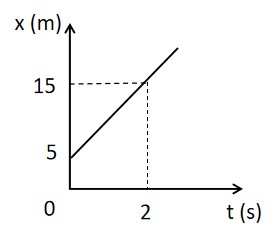
\includegraphics[scale=0.6]{../figs/VN10-PH-03-L-002-4-V2-01.jpg}
		\end{center}
		\begin{mcq}(4)
			\item $x=5+5t$.
			\item $x=4t$.
			\item $x=5-5t$.
			\item $x=5+4t$.
		\end{mcq}
	}
	{\hide{
		Nhận xét rằng đồ thị mô tả chuyển động của vật đi qua các điểm (\SI{0}{\second},\SI{5}{\meter}) và $(\SI{2}{\second},\SI{15}{\meter})$. Vận tốc của vật được tính từ tọa độ các điểm này 
		\begin{equation*}
			v=\dfrac{x-x_0}{t-t_0}=\dfrac{\SI{15}{\meter}-\SI{5}{\meter}}{\SI{2}{\second}-\SI{0}{\second}}=\SI{5}{\meter/\second}.
		\end{equation*}
		
		Phương trình chuyển động của vật do đó có dạng 
		\begin{equation*}
			x=x_0+vt=5+5t\textrm{ (m, s)}.
		\end{equation*}
		
		\textbf{Đáp án: A}.
	}}

	\viduii{3}{	Hai xe chuyển động đều trên cùng một đường thẳng, cùng chiều. Tốc độ của xe (I) là $\SI{20}{\meter/\second}$, tốc độ của xe (II) là $\SI{10}{\meter/\second}$. Lúc $t=0$, hai xe cách nhau $\SI{200}{\meter}$. Chọn gốc tọa độ là vị trí của xe (I) lúc $t=0$, chiều dương là chiều chuyển động của hai xe.
		\begin{enumerate}[label=\alph*)]
			\item Viết phương trình chuyển động của mỗi xe.
			\item Vẽ đồ thị chuyển động của hai xe, từ đồ thị hãy xác định thời điểm và nơi gặp nhau của hai xe.
		\end{enumerate}
	}
	{\hide{
		\begin{enumerate}[label=\alph*)]
			\item
			Hệ quy chiếu gồm:
			\begin{itemize}
				\item Gốc tọa độ là vị trí của xe (I) lúc $t=0$;
				\item Chiều dương là chiều chuyển động của hai xe;
				\item Mốc thời gian ($t=0$) là lúc hai xe cách nhau $\SI{200}{\meter}$.
			\end{itemize}
			
			Phương trình chuyển động của vật (I) là:
			\begin{equation*}
				x_\text{(I)}=x_{0\text{(I)}} + v_\text{(I)}t =20t\textrm{ (m, s)}.
			\end{equation*}
			
			Phương trình chuyển động của vật (II) là:
			\begin{equation*}
				x_\text{(II)}=x_{0\text{(II)}} + v_\text{(II)}t = 200+10t\textrm{ (m, s)}.
			\end{equation*}
			\item
			Đồ thị chuyển động của hai xe là:
			\begin{center}
				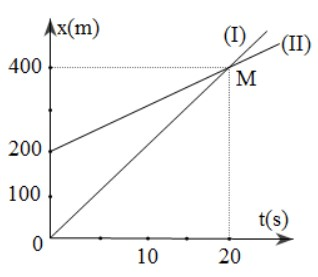
\includegraphics[scale=0.8]{../figs/VN10-PH-03-L-002-4-V2-02.jpg}
			\end{center}
			Hai đồ thị cắt nhau tại M ($t_M=\SI{20}{\second}$, $x_M=\SI{400}{\meter}$). Do đó, nơi gặp cách vị trí xe (I) lúc $t=0$ là $\SI{400}{\meter}$ sau thời gian $\SI{20}{\second}$.
		\end{enumerate}	
	}}
\end{dang}

%				\let\lesson\undefined
\newcommand{\lesson}{\phantomlesson{Bài 4.}}
\setcounter{section}{2}
\section{Bài tập trắc nghiệm}
\begin{enumerate}[label=\bfseries Câu \arabic*:,leftmargin=1.5cm]
	\item \mkstar{1}\\
	Khi vật chuyển động thẳng đều cùng chiều dương thì đồ thị $d - t$ của vật có dạng là
	\begin{mcq}(2)
		\item đường thẳng vuông góc với trục $Od$.
		\item đường thẳng xiên góc đi lên.
		\item đường thẳng xiên góc đi xuống.
		\item đường thẳng vuông góc với trục $Ot$.
	\end{mcq}
\hideall{
\textbf{Đáp án B.}
}
	
	\item \mkstar{2}\\
	{\begin{minipage}[l]{0.65\textwidth}
			Cho đồ thị độ dịch chuyển – thời gian của một vật như hình. Chọn phát biểu đúng.
			\begin{mcq}
				\item Vật đang chuyển động thẳng đều theo chiều dương.
				\item Vật đang chuyển động thẳng đều theo chiều âm.
				\item Vật đang đứng yên.
				\item Vật chuyển động thẳng đều theo chiều dương rồi đổi chiều chuyển động ngược lại.
			\end{mcq}
		\end{minipage}
		\begin{minipage}{0.35\textwidth}
			\begin{center}
				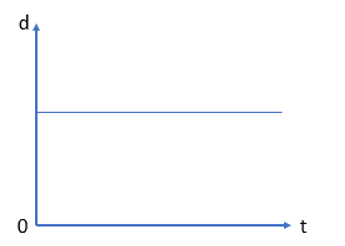
\includegraphics[width=0.7\linewidth]{../figs/VN10-2023-PH-TP005-P-1}
			\end{center}
		\end{minipage}
}
\hideall{
\textbf{Đáp án: C.}
}

\item \mkstar{2}\\
{\begin{minipage}[l]{0.65\textwidth}
		Cho đồ thị độ dịch chuyển – thời gian của một vật như hình. Chọn phát biểu đúng.
		\begin{mcq}
			\item Vật đang chuyển động thẳng đều theo chiều dương.
			\item Vật đang chuyển động thẳng đều theo chiều âm.
			\item Vật đang đứng yên.
			\item Vật chuyển động thẳng đều theo chiều dương rồi đổi chiều chuyển động ngược lại.
		\end{mcq}
	\end{minipage}
	\begin{minipage}{0.35\textwidth}
		\begin{center}
			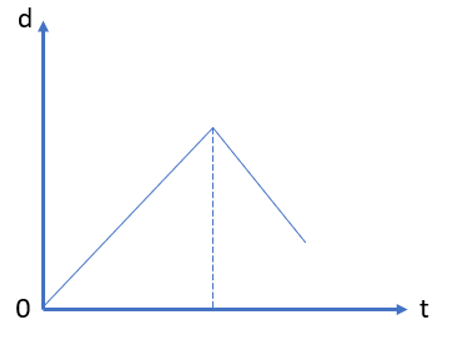
\includegraphics[width=0.7\linewidth]{../figs/VN10-2023-PH-TP005-P-2}
		\end{center}
	\end{minipage}
}
\hideall{
	\textbf{Đáp án: D.}
}

\item \mkstar{2}\\
{Cho đồ thị độ dịch chuyển – thời gian trong chuyển động thẳng của một xe ô tô đồ chơi điều khiển từ xa.\\
		Chọn kết luận \textbf{sai}.
		\begin{center}
			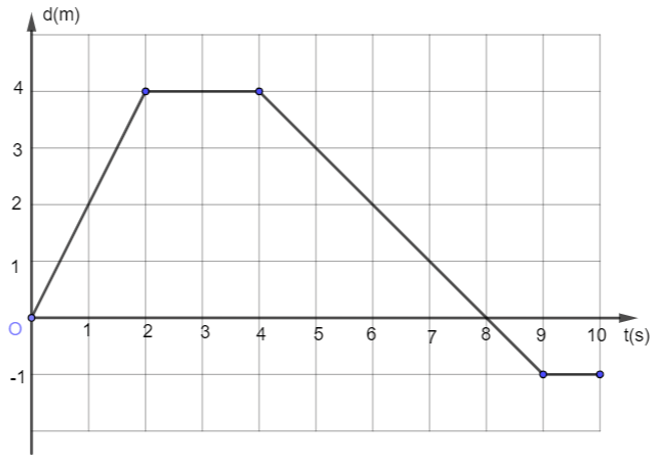
\includegraphics[width=0.5\linewidth]{../figs/VN10-2023-PH-TP005-P-3}
		\end{center}
		\begin{mcq}
			\item Trong 2 giây đầu xe chuyển động vói vận tốc không đổi.
			\item Từ giây thứ 2 đến giây thứ 4 xe dừng lại.
			\item Từ giây thứ 4 đến giây thứ 9 xe đổi chiều chuyển động theo hướng ngược lại với tốc độ nhỏ hơn lúc đi.
			\item Từ giây thứ 9 đến giây thứ 10 xe quay về đúng vị trí xuất phát rồi dừng lại.
		\end{mcq}
}
\hideall{
\textbf{Đáp án: D.}
}

\item \mkstar{2}\\
{Đồ thị độ dịch chuyển – thời gian trong chuyển động thẳng của một chất điểm có dạng như hình vẽ.\\
	\begin{minipage}[l]{0.5\textwidth}
		Trong thời gian nào xe chuyển động thẳng đều?
		\begin{mcq}
			\item Trong khoảng thời gian từ $0$ đến $t_1$.
			\item Trong khoảng thời gian từ $0$ đến $t_2$.
			\item Trong khoảng thời gian từ $t_1$ đến $t_2$.
			\item Không có lúc nào xe chuyển động thẳng đều.
		\end{mcq}
	\end{minipage}
\begin{minipage}{0.5\textwidth}
	\begin{center}
		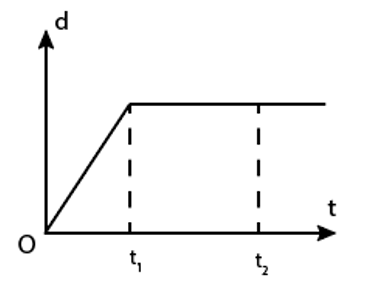
\includegraphics[width=0.5\linewidth]{../figs/VN10-2023-PH-TP005-P-4}
	\end{center}
\end{minipage}
}
\hideall{
\textbf{Đáp án: A.}
}

\item \mkstar{2}\\
{Phương trình chuyển động của một chất điểm dọc theo trục $Ox$ có dạng: $x = 5 + 60t$ ($x$ đo bằng kilomét và $t$ đo bằng giờ). Chất điểm đó xuất phát từ điểm nào và chuyển động với vận tốc bằng bao nhiêu?
	\begin{mcq}
		\item Từ điểm $O$, với vận tốc $\SI{5}{\kilo\meter/\hour}$.
		\item Từ điểm $O$, với vận tốc $\SI{60}{\kilo\meter/\hour}$.
		\item Từ điểm $M$ cách $O$ $\SI{5}{\kilo\meter/\hour}$, với vận tốc $\SI{5}{\kilo\meter/\hour}$.
		\item Từ điểm $M$ cách $O$ $\SI{5}{\kilo\meter/\hour}$, với vận tốc $\SI{60}{\kilo\meter/\hour}$.
	\end{mcq}

}
\hideall{
\textbf{Đáp án: D.}
}

\item \mkstar{2}\\
{Phương trình chuyển động của một chất điểm dọc theo $Ox$ có dạng: $x=5t-12$ (km), với $t$ đo bằng giờ. Độ dời của chất điểm từ $\SI{2}{\hour}$ đến $\SI{4}{\hour}$ là
\begin{mcq}(4)
	\item $\SI{8}{\kilo\meter}$.
	\item $\SI{6}{\kilo\meter}$.
	\item $\SI{10}{\kilo\meter}$.
	\item $\SI{2}{\kilo\meter}$.
\end{mcq}
}
\hideall{
\textbf{Đáp án: C.}
}

\item \mkstar{2}\\
{Phương trình chuyển động của một chất điểm dọc theo trục $Ox$ có dạng: $x = 4 -10t$ ($x$ đo bằng kilomét và $t$ đo bằng giờ). Quãng đường đi được của chất điểm sau $\SI{2}{\hour}$ chuyển động là
	\begin{mcq}(4)
		\item $\SI{-20}{\kilo\meter}$.
		\item $\SI{20}{\kilo\meter}$.
		\item $\SI{-8}{\kilo\meter}$.
		\item $\SI{8}{\kilo\meter}$.
	\end{mcq}
}
\hideall{
\textbf{Đáp án: B.}
}





\item \mkstar{3}\\
{\begin{minipage}[l]{0.6\textwidth}
		Hình vẽ bên là đồ thị độ dịch chuyển - thời gian của một chiếc xe ô tô chạy từ $A$ đến $B$ trên một đường thẳng. Vận tốc của xe bằng
		\begin{mcq}
			\item $\SI{30}{\kilo\meter/\hour}$.
			\item $\SI{150}{\kilo\meter/\hour}$.
			\item $\SI{120}{\kilo\meter/\hour}$.
			\item $\SI{100}{\kilo\meter/\hour}$.
		\end{mcq}
	\end{minipage}
\begin{minipage}{0.4\textwidth}
		\begin{center}
			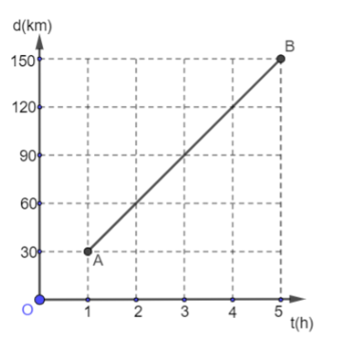
\includegraphics[width=0.6\linewidth]{../figs/VN10-2023-PH-TP005-P-5}
		\end{center}
	\end{minipage}
}
\hideall{
\textbf{Đáp án: A.}\\
Vận tốc của xe 
$$v=\dfrac{d}{\Delta t}=\dfrac{150-30}{5-1}=\SI{30}{\kilo\meter/\hour}.$$
}


\item \mkstar{3}\\
{\begin{minipage}[l]{0.6\textwidth}
		Đồ thị độ dịch chuyển – thời gian của một vật chuyển động như hình vẽ. Vật chuyển động
		\begin{mcq}
			\item ngược chiều dương với tốc độ $\SI{20}{\kilo\meter/\hour}$.
			\item cùng chiều dương với tốc độ $\SI{20}{\kilo\meter/\hour}$.
			\item ngược chiều dương với tốc độ $\SI{60}{\kilo\meter/\hour}$.
			\item cùng chiều dương với tốc độ $\SI{60}{\kilo\meter/\hour}$.
		\end{mcq}
	\end{minipage}
	\begin{minipage}{0.4\textwidth}
		\begin{center}
			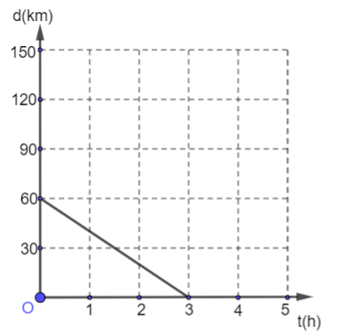
\includegraphics[width=0.6\linewidth]{../figs/VN10-2023-PH-TP005-P-6}
		\end{center}
	\end{minipage}
}
\hideall{
	\textbf{Đáp án: A.}\\
	Vật dịch chuyển ngược chiều dương với tốc độ
	$$v=\dfrac{s}{t}=\dfrac{60}{3}=\SI{20}{\kilo\meter/\hour}.$$
}

\item \mkstar{3}\\
{\begin{minipage}[l]{0.6\textwidth}
		Một chất điểm chuyển động trên một đường thẳng. Đồ thị độ dịch chuyển theo thời gian của chất điểm được mô tả như hình vẽ. Tốc độ trung bình của chất điểm trong khoảng thời gian từ 0 đến $\SI{5}{\second}$ là
		\begin{mcq}(2)
			\item $\SI{1.6}{\centi\meter/\second}$.
			\item $\SI{6.4}{\centi\meter/\second}$.
			\item $\SI{4.8}{\centi\meter/\second}$.
			\item $\SI{2.4}{\centi\meter/\second}$.
		\end{mcq}
	\end{minipage}
	\begin{minipage}{0.4\textwidth}
		\begin{center}
			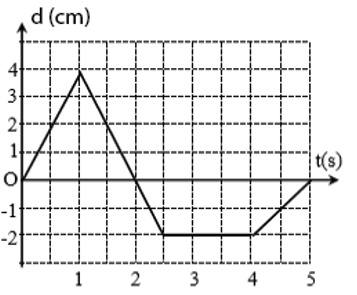
\includegraphics[width=0.6\linewidth]{../figs/VN10-2023-PH-TP005-P-7}
		\end{center}
	\end{minipage}
}
\hideall{
	\textbf{Đáp án: D.}\\
	Tốc độ trung bình của chất điểm:
	$$v_\text{tb}=\dfrac{s}{t}=\dfrac{4+4+2+2}{5}=\SI{2.4}{\centi\meter/\second}.$$
}

\item \mkstar{3}\\
{Một người đi bằng thuyền với tốc độ $\SI{2}{\meter/\second}$ về phía đông. Sau khi đi được $\SI{2.2}{\kilo\meter}$, người này lên ô tô đi về phía bắc trong 15 phút với tốc độ $\SI{60}{\kilo\meter/\hour}$. Hãy chọn kết luận \textbf{sai}.
	\begin{mcq}(2)
		\item Tổng quãng đường đã đi là $\SI{17.2}{\kilo\meter}$.
		\item Độ dịch chuyển là $\SI{15.2}{\kilo\meter}$.
		\item Tốc độ trung bình là $\SI{8.6}{\meter/\second}$.
		\item Vận tốc trung bình bằng $\SI{8.6}{\meter/\second}$.
	\end{mcq}
}
\hideall{
	\textbf{Đáp án: D.}\\
	Tổng thời gian dịch chuyển: 
	$$t=\dfrac{s_1}{v_1}+t_2=\xsi{\dfrac{5}{9}}{\hour}$$
	Vận tốc trung bình $$v=\dfrac{d}{t}=\dfrac{\SI{15.2}{\kilo\meter}}{\xsi{\dfrac{5}{9}}{\hour}}=\SI{27.36}{\kilo\meter/\hour}=\SI{7.6}{\meter/\second}.$$
	
}

\item \mkstar{3}\\
{Một người bơi dọc theo chiều dài $\SI{100}{\meter}$ của bể bơi hết $\SI{60}{\second}$ rồi quay về lại chỗ xuất phát trong $\SI{70}{\second}$. Trong suốt quãng đường đi và về tốc độ trung bình, vận tốc trung bình của người đó lần lượt là
\begin{mcq}(4)
	\item $\SI{1.538}{\meter/\second}$; $\SI{0}{\meter/\second}$.
	\item $\SI{1.538}{\meter/\second}$; $\SI{1.876}{\meter/\second}$.
	\item $\SI{3.077}{\meter/\second}$; $\SI{2}{\meter/\second}$.
	\item $\SI{7.692}{\meter/\second}$; $\SI{2.2}{\meter/\second}$.
\end{mcq}
}
\hideall{
\textbf{Đáp án: A.}\\
Quãng đường và độ dịch chuyển của người bơi:
$$s=2\ell=\SI{200}{\meter}; d=0$$
Tốc độ trung bình:
$$v_\text{tb}=\dfrac{s}{t}=\SI{1.538}{\meter/\second}$$
Vận tốc trung bình:
$$v=\dfrac{d}{t}=0.$$
}


\item \mkstar{3}\\
{Lúc $\SI{7}{\hour}$, ô tô thứ nhất đi qua điểm $A$, ô tô thứ hai đi qua điểm $B$ cách $A$ $\SI{10}{\kilo\meter}$. Xe đi qua $A$ với vận tốc $\SI{50}{\kilo\meter/\hour}$, xe đi qua $B$ với vận tốc $\SI{40}{\kilo\meter/\hour}$. Biết hai xe chuyển động cùng chiều theo hướng từ $A$ đến $B$. Coi chuyển động của 2 ô tô là chuyển động đều. Hỏi
\begin{enumerate}[label=\alph*)]
	\item Hai xe gặp nhau lúc mấy giờ?
	\begin{mcq}(4)
		\item 7h30.
		\item 8h.
		\item 9h.
		\item 8h30.
	\end{mcq}
\item Quãng đường xe $A$ đã đi được đến khi gặp xe $B$ là
\begin{mcq}(4)
	\item $\SI{80}{\kilo\meter}$.
	\item $\SI{40}{\kilo\meter}$.
	\item $\SI{50}{\kilo\meter}$.
	\item $\SI{90}{\kilo\meter}$.
\end{mcq}
\item Hai xe cách nhau 20 km lúc mấy giờ?
\begin{mcq}(4)
	\item 9h.
	\item 9h30.
	\item 10h.
	\item 11h.
\end{mcq}
\end{enumerate}
}
\hideall{
\textbf{Đáp án: B - C - C.}
Chọn gốc toạ độ tại A, chiều dương hướng từ A sang B, gốc thời gian lúc $\SI{7}{\hour}$.\\
Phương trình chuyển động của mỗi xe:
\begin{align*}
	\begin{cases}
		x_1=50t\\
		x_2=10+40t
	\end{cases}
\end{align*}
Hai xe gặp nhau thì $x_1=x_2\Rightarrow t=\SI{1}{\hour}$.\\
Vậy hai xe gặp nhau lúc $\SI{8}{\hour}$.\\
Quãng đường xe A đi được:
$$s_A=v_A\cdot t=\SI{50}{\kilo\meter}$$
Thời điểm hai xe cách nhau $\SI{20}{\kilo\meter}$:
$$\left|x_1-x_2\right|=20\Rightarrow t=\SI{3}{\hour}$$
Vậy hai xe cách nhau $\SI{20}{\kilo\meter}$ lúc $\SI{10}{\hour}$.
}

\item \mkstar{3}\\
{Hãy viết phương trình chuyển động của một ô tô chuyển động thẳng đều biết rằng tại $t_1=\SI{2}{\hour}$ thì $x_1=\SI{40}{\kilo\meter}$ và tại $t_2 =\SI{3}{\hour}$ thì $x_2=\SI{90}{\kilo\meter}$.
	\begin{mcq}(2)
		\item $x=-60+50t\qquad\left(\si{\kilo\meter}, \si{\hour}\right)$.
		\item $x=-60+30t\qquad\left(\si{\kilo\meter}, \si{\hour}\right)$.
		\item $x=-60+40t\qquad\left(\si{\kilo\meter}, \si{\hour}\right)$.
		\item $x=-60+20t\qquad\left(\si{\kilo\meter}, \si{\hour}\right)$.
	\end{mcq}
}
\hideall{
\textbf{Đáp án: A.}\\
Phương trình chuyển động của vật:
$$x=x_0+vt$$
Khi $t=t_1=\SI{2}{\hour}$ thì $x=x_1=\SI{40}{\kilo\meter}$ và khi $t=t_2=\SI{3}{\hour}$ thì $x=x_2=\SI{90}{\kilo\meter}$.
\begin{align*}
	\begin{cases}
		40=x_0+2v\\
		90=x_0+3v
	\end{cases}
\Rightarrow
\begin{cases}
	x_0=\SI{-60}{\kilo\meter}\\
	v=\SI{50}{\kilo\meter/\hour}
\end{cases}
\end{align*}
}

\item \mkstar{3}\\
{Hãy thiết lập phương trình chuyển động của một ô tô chuyển động thẳng đều biết. Ô tô chuyển động theo chiều dương với vận tốc $\SI{10}{\meter/\second}$ và ở thời điểm $\SI{3}{\second}$ thì ô tô có tọa độ $\SI{60}{\meter}$.
\begin{mcq}(2)
	\item $x=30+10t\qquad\left(\si{\meter}, \si{\second}\right)$.
	\item $x=20+10t\qquad\left(\si{\meter}, \si{\second}\right)$.
	\item $x=10+20t\qquad\left(\si{\meter}, \si{\second}\right)$.
	\item $x=40+10t\qquad\left(\si{\meter}, \si{\second}\right)$.
\end{mcq}
}
\hideall{
\textbf{Đáp án: A.}\\
Phương trình chuyển động của ô tô:
$$x=x_0+10t$$
Tại $t=\SI{3}{\second}$ thì $x=\SI{60}{\meter} \Rightarrow x_0=\SI{30}{\meter}$.
}

\item \mkstar{3}\\
{Hai trạm dừng chân $A$ và $B$ cách nhau $\SI{72}{\kilo\meter}$. Lúc 7h30 sáng, xe ô tô 1 khởi hành từ $A$ chuyển động thẳng đều về $B$ với tốc độ $\SI{36}{\kilo\meter/\hour}$. Nửa giờ sau, xe ô tô 2 chuyển động thẳng đều từ $B$ đến $A$ và gặp ô tô 1 lúc 8 giờ 30 phút. Tìm tốc độ của xe ô tô thứ hai.
	\begin{mcq}(4)
		\item $v_2=\SI{70}{\kilo\meter/\hour}$.
		\item $v_2=\SI{72}{\kilo\meter/\hour}$.
		\item$v_2=\SI{73}{\kilo\meter/\hour}$.
		\item $v_2=\SI{74}{\kilo\meter/\hour}$.
	\end{mcq}

}
\hideall{
\textbf{Đáp án: B.}\\
Phương trình chuyển động của mỗi ô tô
\begin{align*}
	\begin{cases}
		x_1=36t\\
		x_2=72-v_2\cdot\left(t-0.5\right)
	\end{cases}
\end{align*}
Hai xe gặp nhau sau khoảng thời gian $t=\SI{1}{\hour}\Rightarrow v_2=\SI{72}{\kilo\meter/\hour}$.
}

\item \mkstar{3}\\
{Lúc 7 giờ một người đang ở $A$ chuyển động thẳng đều với vận tốc $\SI{10}{\meter/\second}$ đuổi theo người ở $B$ đang chuyển động thẳng đều với vận tốc $\SI{18}{\kilo\meter/\hour}$. Biết $AB =\SI{36}{\kilo\meter}$. Chọn trục tọa độ trùng với quỹ đạo chuyển động, chiều dương là chiều chuyển động, gốc tọa độ tại A, gốc thời gian là lúc $\SI{7}{\hour}$. Thời điểm và vị trí người thứ nhất đuổi kịp người thứ hai là
\begin{mcq}(2)
	\item lúc $\SI{2}{\hour}$ cách $A$ $\SI{72}{\kilo\meter}$.
	\item lúc $\SI{9}{\hour}$ cách $B$ $\SI{36}{\kilo\meter}$.
	\item lúc $\SI{9}{\hour}$ cách $A$ $\SI{72}{\kilo\meter}$.
	\item lúc $\SI{2}{\hour}$ cách $B$ $\SI{36}{\kilo\meter}$.
\end{mcq}
}
\hideall{
\textbf{Đáp án: C.}\\
Phương trình chuyển động cảu mỗi người
\begin{align*}
	\begin{cases}
		x_A=36t\\
		x_B=36+18t
	\end{cases}
\end{align*}
Hai người gặp nhau $x_A=x_B\Rightarrow t=\SI{2}{\hour}$\\
Vị trí gặp nhau cách A đoạn $x_A=\SI{72}{\kilo\meter}$.
}

\item \mkstar{3}\\
{Lúc $\SI{10}{\hour}$ có một xe xuất phát từ $A$ đi về $B$ với tốc độ $\SI{50}{\kilo\meter/\hour}$. Lúc 10h30 một xe khác xuất phát từ $B$ đi về $A$ với tốc độ $\SI{80}{\kilo\meter/\hour}$. Cho $AB =\SI{200}{\kilo\meter}$. Lúc $\SI{11}{\hour}$, hai xe cách nhau
\begin{mcq}(4)
	\item $\SI{100}{\kilo\meter}$.
	\item $\SI{110}{\kilo\meter}$.
	\item $\SI{150}{\kilo\meter}$.
	\item $\SI{160}{\kilo\meter}$.
\end{mcq}
}
\hideall{
\textbf{Đáp án: B.}\\
Phương trình chuyển động của mỗi xe
\begin{align*}
	\begin{cases}
		x_A=50t\\
		x_B=200-80\cdot\left(t-0,5\right)
	\end{cases}
\end{align*}
Khoảng cách giữa hai người lúc $\SI{11}{\hour}$
$$\Delta x=\left|x_A-x_B\right|$$
Với $t=\SI{1}{\hour}$ thì $\Delta x=\SI{110}{\kilo\meter}$.
}

\item \mkstar{4}\\
{\begin{minipage}[l]{0.6\textwidth}
		Hình dưới là đồ thị độ dịch chuyển - thời gian của hai vật chuyển động thẳng cùng hướng. Tỉ lệ vận tốc $\dfrac{v_A}{v_B}$ là
		\begin{mcq}(2)
			\item $\dfrac{3}{1}$.
			\item $\dfrac{1}{3}$.
			\item $\dfrac{\sqrt{3}}{1}$.
			\item $\dfrac{1}{\sqrt{3}}$.
		\end{mcq}
	\end{minipage}
	\begin{minipage}{0.4\textwidth}
		\begin{center}
			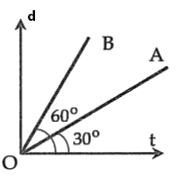
\includegraphics[width=0.4\linewidth]{../figs/VN10-2023-PH-TP005-P-8}
		\end{center}
	\end{minipage}
}
\hideall{
	\textbf{Đáp án: B.}\\
	$$\dfrac{v_A}{v_B}=\dfrac{\tan\SI{30}{\degree}}{\tan\SI{60}{\degree}}=\dfrac{1}{3}.$$
}


\end{enumerate}
\section{Bài tập tự luận}
\begin{enumerate}[label=\bfseries Bài \arabic*:,leftmargin=1.5cm]
		\item \mkstar{3}\\
	{
		Hãy tính quãng đường đi được, độ dịch chuyển, tốc độ, vận tốc của bạn A khi đi từ nhà đến trường và khi đi từ trường đến siêu thị. Coi chuyển động của bạn A là chuyển động đều và biết cứ $\SI{100}{m}$ bạn A đi hết $\SI{25}{s}$.
		\begin{center}
			\includegraphics[scale=0.9]{../figs/VN10-2022-PH-TP006-1.jpg}
		\end{center}
	}
	
	\hideall{
		
		Vì bạn A đi từ nhà đến trường là theo 1 hướng, không đổi hướng nên :
		
		Quãng đường đi được và độ dịch chuyển là như nhau và bằng $\SI{1000}{m}$.
		
		Vận tốc và tốc độ là như nhau và bằng : 
		
		$$v = \dfrac{d}{t} =\dfrac{100}{25} = \SI{4}{m/s}.$$
		Tương tự, khi đi từ trường đến siêu thị thì quãng đường và độ dịch chuyển bằng nhau và bằng $\SI{200}{\meter}$.
	}

	\item \mkstar{3}\\
	{
		Bạn A đi học từ nhà đến trường theo lộ trình ABC. Biết bạn A đi đoạn đường $\text{AB} = \SI{400}{m}$ hết 6 phút, đoạn đường $\text{BC} = \SI{300}{m}$ hết 4 phút. Xác định tốc độ trung bình và vận tốc trung bình của bạn A khi đi từ nhà đến trường.
		\begin{center}
			\includegraphics[scale=1]{../figs/VN10-2022-PH-TP005-2.jpg}
		\end{center}
	}
	\hideall
	{
		Độ dịch chuyển của bạn A đến trường chính là độ dài
		
		$$\text{AC} = \sqrt{(\text{AB})^2 + (\text{BC})^2} = \SI{500}{m}.$$
		
		Tốc độ trung bình 
		
		$$v= \dfrac{s}{t} = \dfrac{300+400}{(6 + 4)60}  = \SI{1,17}{m/s}.$$
		
		Vận tốc trung bình
		
		$$v'=\dfrac{d}{t}=\dfrac{500}{(6+4)60} = \SI{0,83}{m/s}.$$
	}

	\item \mkstar{2}
	
	{
		Hãy vẽ đồ thị độ dịch chuyển - thời gian trong chuyển động của A theo bảng ghi số liệu vào vở. Trên trục tung (trục độ dịch chuyển) $\SI{1}{cm}$ ứng với $\SI{200}{m}$; trên trục hoành (trục thời gian) $\SI{1}{cm}$ ứng với $\SI{50}{s}$.
		
		\begin{center}
			\includegraphics[scale=1]{../figs/VN10-2022-PH-TP006-5.jpg}
		\end{center}
		
	}
	\hideall{
		
		Từ bảng số liệu ta vẽ được đồ thị như hình sau:
		
		
		\begin{center}
			\includegraphics[scale=0.6]{../figs/VN10-2022-PH-TP006-6.jpg}
		\end{center}
		
	}
	

	\item \mkstar{3}
	
	{
		Đồ thị độ dịch chuyển - thời gian của một người đang bơi trong một bể bơi dài $\SI{50}{m}$. 
		\begin{center}
			\includegraphics[scale=1]{../figs/VN10-2022-PH-TP006-2.jpg}
		\end{center}
	\begin{enumerate}[label=\alph*)]
		\item Trong 25 giây đầu mỗi giây người đó bơi được bao nhiêu mét? Tính vận tốc của người đó ra m/s. Từ giây nào đến giây nào người đó không bơi?
		\item Từ giây 35 đến giây 60 người đó bơi theo chiều nào? Trong 20 giây cuối cùng, mỗi giây người đó bơi được bao nhiêu mét? Tính vận tốc của người đó ra m/s.
		\item Xác định độ dịch chuyển và vận tốc của người đó trong cả quá trình bơi.
	\end{enumerate}
}
	\hideall{
		\begin{enumerate}[label=\alph*)]
			\item Từ đồ thị ta thấy, trong 25 giây đầu người đó chuyển động thẳng từ O – A và không đổi chiều, độ dịch chuyển trong 25 giây đầu là $\SI{50}{m}$.
			
			Mỗi giây người đó bơi được:
			
			$$\dfrac{50}{25} = \SI{2}{m}.$$
			
			Vận tốc của người đó:
			
			$$v = \dfrac{d}{t} = \dfrac{50}{25} = \SI{2}{m/s}.$$
			
			Từ A – B: người đó không bơi $\Rightarrow$ Người đó không bơi từ giây 25 đến giây 35.
			\item Từ giây 35 đến giây 60 người đó bơi ngược chiều dương.
			
			Trong 20 giây cuối cùng:
			
			Từ đồ thị ta thấy
			\begin{itemize}
				\item Giây thứ 40 có $d_1 = \SI{45}{m}$.
				\item Giây thứ 60 có $d_2 =  \SI{25}{m}$.\\
				$\Rightarrow$ Trong 20 giây cuối, mỗi giây người đó bơi được 
				
				$$\dfrac{|25 - 15|}{20} = \SI{1}{m}.$$
				\item Vận tốc của người đó là
					$$v = \dfrac{\Delta d}{\Delta t} = \dfrac{d_2 - d_1}{\Delta t} = -\SI{1}{m/s}.$$
			\end{itemize}
		\end{enumerate}		
	}
	
	\item \mkstar{3}
	
	{
		Số liệu về độ dịch chuyển và thời gian của chuyển động thẳng của một xe ô tô đồ chơi chạy bằng pin được ghi trong bảng bên: 
		\begin{center}
			\includegraphics[scale=1]{../figs/VN10-2022-PH-TP006-3.jpg}
		\end{center}
		
		Dựa vào bảng để:
		
		\begin{enumerate}[label=\alph*)]
			\item Vẽ đồ thị độ dịch chuyển - thời gian của chuyển động.
			\item Mô tả chuyển động của xe.
			\item Tính vận tốc của xe trong $\SI{3}{s}$ đầu.
		\end{enumerate}
	}
	\hideall{
		
		\begin{enumerate}[label=\alph*)]
			\item Vẽ đồ thị độ dịch chuyển - thời gian của chuyển động
			
			\begin{center}
				\includegraphics[scale=0.6]{../figs/VN10-2022-PH-TP006-7.jpg}
			\end{center}
			
			\item Mô tả chuyển động của xe
			
			- Từ 0 – 3 giây: xe chuyển động thẳng.
			
			- Từ giây thứ 3 đến giây thứ 5: xe đứng yên (dừng lại).
			
			
			\item 
			Độ dịch chuyển của xe trong 3 giây đầu là:
			
			$$d = 7-1 = \SI{6}{m}.$$
			
			Vận tốc của xe trong $\SI{3}{s}$ đầu
			
			$$v = \dfrac{\Delta d}{\Delta t} = \SI{2}{m/s}.$$
			
		\end{enumerate}
	}
	\item \mkstar{3}
	
	{
		Đồ thị độ dịch chuyển - thời gian trong chuyển động thẳng của một xe ô tô đồ chơi điều khiển từ xa được vẽ ở hình: 
		\begin{center}
			\includegraphics[scale=1]{../figs/VN10-2022-PH-TP006-4.jpg}
		\end{center}
		
		
		\begin{enumerate}[label=\alph*)]
			\item Mô tả chuyển động của xe.
			\item Xác định vị trí của xe so với điểm xuất phát của xe ở giây thứ 2, giây thứ 4, giây thứ 8 và giây thứ 10.
			\item Xác định tốc độ và vận tốc của xe trong 2 giây đầu, từ giây 2 đến giây 4 và từ giây 4 đến giây 8.
			\item Xác định quãng đường đi được và độ dịch chuyển của xe sau 10 giây chuyển động. Tại sao giá trị của chúng không giống nhau?
		\end{enumerate}
	}
	\hideall{
		
		\begin{enumerate}[label=\alph*)]
			\item Mô tả chuyển động của xe
			
			- Trong 2 giây đầu: xe chuyển động thẳng
			
			- Từ giây thứ 2 đến giây thứ 4: xe đứng yên
			
			- Từ giây thứ 4 đến giây thứ 10: xe chuyển động thẳng theo chiều ngược lại.
			
			- Từ giây thứ 9 đến giây thứ 10: xe dừng lại.
			
			\item 
			
			- Ở giây thứ 2: xe ở vị trí cách điểm xuất phát $\SI{4}{m}$.
			
			- Ở giây thứ 4: xe ở vị trí cách điểm xuất phát $\SI{4}{m}$.
			
			- Ở giây thứ 8: xe trở về vị trí xuất phát.
			
			- Ở giây thứ 10: xe ở vị trí cách điểm xuất phát $\SI{1}{m}$ theo chiều âm.
			\item Xác định tốc độ và vận tốc của xe
			
			- Trong 2 giây đầu, xe chuyển động thẳng, không đổi chiều nên tốc độ bằng vận tốc:
			
			$$v = \dfrac{d}{t} = \SI{2}{m/s}.$$
			
			- Từ giây 2 đến giây 4: xe đứng yên nên vận tốc và tốc độ của xe đều bằng 0.
			
			- Từ giây 4 đến giây 8:
			
			+ Tốc độ:
			
			$$v = \dfrac{s}{t} = \SI{1}{m/s}.$$
			
			+ Vận tốc:
			
			$$v = \dfrac{\Delta d}{\Delta t} = -\SI{1}{m/s}.$$
			\item
			- Từ đồ thị, ta thấy quãng đường đi được của xe sau 10 giây chuyển động là:
			
			$$s = 4 + 4 + 1 = \SI{9}{m}.$$
			
			- Độ dịch chuyển của xe sau 10 giây là:
			
			$$d = - 1 - 4 + 4 = - \SI{1}{m}.$$
			
			Suy ra quãng đường và độ dịch chuyển của xe sau 10 giây không giống nhau vì xe chuyển động theo 2 chiều.
		\end{enumerate}
	}
	
\end{enumerate}
%			\stopMyChapterToc
%		\mychapter[Chuyển động tổng hợp]{Chuyển động tổng hợp}
%			\startMyChapterToc
%				\let\lesson\undefined
\newcommand{\lesson}{\phantomlesson{Bài 5: Chuyển động tổng hợp}}
\chapter[Chuyển động tổng hợp]{Chuyển động tổng hợp}
\setcounter{section}{0}
\section{Lý thuyết}
\subsection{Tính tương đối của chuyển động}
Một vật có thể xem như là đứng yên trong hệ quy chiếu này, nhưng lại chuyển động trong hệ quy chiếu khác. Do đó, chuyển động có tính tương đối.
\subsubsection{Quỹ đạo có tính tương đối}
Hình dạng của quỹ đạo của chuyển động trong các hệ quy chiếu khác nhau thì khác nhau. 
\subsubsection{Vận tốc có tính tương đối}
Vận tốc của chuyển động với các hệ quy chiếu khác nhau thì khác nhau. 
\subsection{Hệ quy chiếu đứng yên và hệ quy chiếu chuyển động}
\begin{itemize}
	\item \textbf{Hệ quy chiếu đứng yên:} là hệ quy chiếu gắn với vật làm mốc được quy ước là đứng yên.\\
	\textit{\textbf{Ví dụ:}} Hệ quy chiếu gắn với sân ga, hệ quy chiếu gắn với bờ sông, \dots
	\item \textbf{Hệ quy chiếu chuyển động:} là hệ quy chiếu gắn với vật làm gốc chuyển động so với hệ quy chiếu đứng yên.\\
	\textit{\textbf{Ví dụ:}} hệ quy chiếu gắn với tàu hoà đang chuyển động, hệ quy chiếu gắn với dòng nước đang trôi, \dots
\end{itemize}
\subsection{Độ dịch chuyển tổng hợp - Vận tốc tổng hợp}
Quy ước:
\begin{itemize}
	\item Vật số 1 (người) là vật chuyển động đang được xét.
	\item Vật số 2 (toa tàu) là vật chuyển động được chọn làm gốc của hệ quy chiếu chuyển động.
	\item Vật số 3 (đường ray) là vật đứng yên được chọn làm gốc của hệ quy chiếu đứng yên
\end{itemize}
\begin{center}
	\includegraphics[width=0.6\linewidth]{../figs/VN10-2023-PH-TP006-1}
\end{center}
Khi vật 1 có độ dịch chuyển $\overrightarrow{d_{12}}$ trong hệ quy chiếu chuyển động, đồng thời hệ quy chiếu chuyển động cũng có độ dịch chuyển $\overrightarrow{d_{23}}$ so với hệ quy chiếu đứng yên. Do đó, độ dịch chuyển tổng hợp:
$$\overrightarrow{d_{13}}=\overrightarrow{d_{12}}+\overrightarrow{d_{23}}$$
Xét trong khoảng thời gian $\Delta t$ rất bé và kết hợp với định nghĩa của vận tốc:
$$\dfrac{\overrightarrow{d_{13}}}{\Delta t}=\dfrac{\overrightarrow{d_{12}}}{\Delta t}+\dfrac{\overrightarrow{d_{23}}}{\Delta t}$$
$$\Rightarrow \overrightarrow{v_{13}}=\overrightarrow{v_{12}}+\overrightarrow{v_{23}}$$
Trong đó:
\begin{itemize}
	\item $\overrightarrow{v_{13}}$: vận tốc tuyệt đối (vận tốc của vật đối với hệ quy chiếu đứng yên);
	\item $\overrightarrow{v_{12}}$: vận tốc tương đối (vận tốc của vật đối với hệ quy chiếu chuyển động);
	\item $\overrightarrow{v_{23}}$: vận tốc kéo theo (vận tốc của hệ quy chiếu chuyển động đối với hệ quy chiếu đứng yên).
\end{itemize}
\textbf{Trường hợp 1:} $\overrightarrow{v_{12}}\upuparrows \overrightarrow{v_{23}}$
	\begin{center}
		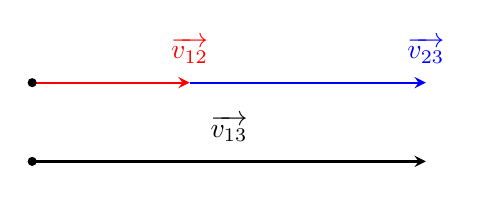
\begin{tikzpicture}
			\coordinate (O) at (0,0);
			\coordinate (B) at (2,0);
			\coordinate (C) at (5,0);
			\coordinate (D) at (2.5,0);
			\coordinate (O1) at ($(O)-(0,1cm)$);
			\coordinate (C1) at ($(C)-(0,1cm)$);
			\coordinate (D1) at ($(D)-(0,1cm)$);
			\draw[-stealth,thick, red] (O) -- (B);
			\draw[-stealth,thick, blue] (B) -- (C);
			\draw[-stealth,thick] (O1) -- (C1);
			\foreach \i in {O,O1}{
				\filldraw[black] (\i) circle (0.5mm);
			}
			\node[label={[red]90:$\overrightarrow{v_{12}}$}] at (B){};	
			\node[label={[blue]90:$\overrightarrow{v_{23}}$}] at (C){};	
			\node[label=90:$\overrightarrow{v_{13}}$] at (D1){};	
		\end{tikzpicture}
	\end{center}
$$v_{13}=v_{12}+v_{23}$$
\textbf{Trường hợp 2:} $\overrightarrow{v_{12}}\uparrow\downarrow \overrightarrow{v_{23}}$
\begin{center}
	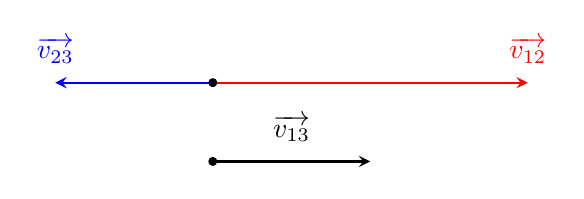
\begin{tikzpicture}
		\coordinate (O) at (0,0);
		\coordinate (B) at (4,0);
		\coordinate (C) at (-2,0);
		\coordinate (D) at (2,0);
		\coordinate (E) at (1,0);
		\coordinate (O1) at ($(O)-(0,1cm)$);
		\coordinate (D1) at ($(D)-(0,1cm)$);
		\coordinate (E1) at ($(E)-(0,1cm)$);
		\draw[-stealth,thick, red] (O) -- (B);
		\draw[-stealth,thick, blue] (O) -- (C);
		\draw[-stealth,thick] (O1) -- (D1);
		\foreach \i in {O,O1}{
			\filldraw[black] (\i) circle (0.5mm);
		}
		\node[label={[red]90:$\overrightarrow{v_{12}}$}] at (B){};	
		\node[label={[blue]90:$\overrightarrow{v_{23}}$}] at (C){};	
		\node[label=90:$\overrightarrow{v_{13}}$] at (E1){};	
	\end{tikzpicture}
\end{center}
$$v_{13}=\left|v_{12}-v_{23}\right|$$
\textbf{Trường hợp 3:} $\overrightarrow{v_{12}} \bot \overrightarrow{v_{23}}$
\begin{center}
	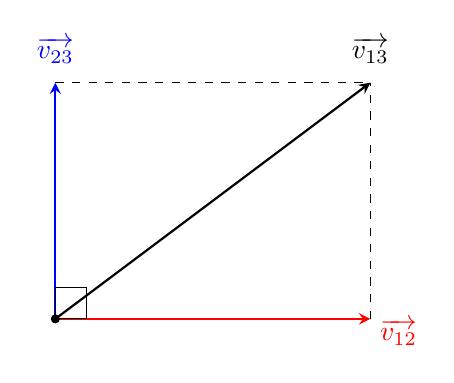
\begin{tikzpicture}
		\coordinate (O) at (0,0);
		\coordinate (B) at (4,0);
		\coordinate (C) at (0,3);
		\coordinate (D) at (4,3);
		\coordinate (E) at (1,0);
		\coordinate (O1) at ($(O)-(0,1cm)$);
		\coordinate (D1) at ($(D)-(0,1cm)$);
		\coordinate (E1) at ($(E)-(0,1cm)$);
		\draw[-stealth,thick, red] (O) -- (B);
		\draw[-stealth,thick, blue] (O) -- (C);
		\draw[-stealth,thick] (O) -- (D);
		\draw[dashed] (B) -- (D);
		\draw[dashed] (C) -- (D);
		\foreach \i in {O}{
			\filldraw[black] (\i) circle (0.5mm);
		}
		\tkzMarkRightAngle[draw=black,size=.4](B,O,C);
		\node[label={[red,below right]90:$\overrightarrow{v_{12}}$}] at (B){};	
		\node[label={[blue]90:$\overrightarrow{v_{23}}$}] at (C){};	
		\node[label=90:$\overrightarrow{v_{13}}$] at (D){};	
	\end{tikzpicture}
\end{center}
$$v_{13}=\sqrt{v^2_{12}+v^2_{23}}$$
\textbf{Trường hợp 4:} $\left(\overrightarrow{v_{12}},\overrightarrow{v_{23}}\right)=\alpha$
\begin{center}
	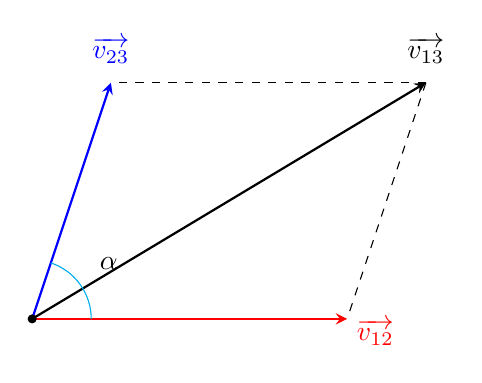
\begin{tikzpicture}
		\coordinate (O) at (0,0);
		\coordinate (B) at (4,0);
		\coordinate (C) at (5,3);
		\coordinate (D) at (1,3);
		\draw[-stealth,thick, red] (O) -- (B);
		\draw[-stealth,thick, blue] (O) -- (D);
		\draw[-stealth,thick] (O) -- (C);
		\draw[dashed] (C) -- (D);
		\draw[dashed] (C) -- (B);
		\foreach \i in {O}{
			\filldraw[black] (\i) circle (0.5mm);
		}
		\node[label={[red,below right]90:$\overrightarrow{v_{12}}$}] at (B){};	
		\node[label={[blue]90:$\overrightarrow{v_{23}}$}] at (D){};	
		\node[label=90:$\overrightarrow{v_{13}}$] at (C){};	
		\tkzMarkAngle[size=0.75cm,color=cyan](B,O,D);
		\tkzLabelAngle[color=black,pos=1.2](B,O,D){$\alpha$}
	\end{tikzpicture}
$$v_{13}=\sqrt{v^2_{12}+v^2_{23}+2v_{12}\cdot v_{23\cdot}\cos\alpha}$$
Nếu $v_{12}=v_{23}$ thì $v_{13}=2v_{12}\cdot\cos\dfrac{\alpha}{2}$.
\end{center}
\section{Mục tiêu bài học - Ví dụ minh họa}

\begin{dang}{Phân biệt vật chuyển động và đứng yên\\ trong các hệ quy chiếu khác nhau}
	\viduii{3}{Một hành khách ngồi trên toa tàu A, nhìn qua cửa sổ thấy toa tàu B bên cạnh và gạch lát sân ga đều chuyển động như nhau. Nếu lấy vật mốc là nhà ga thì:
		\begin{mcq}(2)
			\item Cả hai tàu đều đứng yên.
			\item Tàu B đứng yên, tàu A chuyển động.
			\item Tàu A đứng yên, tàu B chạy.
			\item Cả hai tàu đều chạy.
		\end{mcq}
		
	}
	{\hide{
		Khi hành khách ngồi trên toa tàu A, mà thấy toa tàu B bên cạnh và gạch lát sân ga đều chuyển động như nhau thì tàu B và sân ga cùng trạng thái chuyển động so với tàu A.
		
		Nếu lấy vật mốc là nhà ga, gạch lát sân ga đứng yên nên tàu B cũng đứng yên. Sân ga chuyển động so với tàu A đồng nghĩa với tàu A chuyển động so với sân ga. 
		
		Vậy trong hệ qui chiếu  gắn với sân ga (lấy vật mốc là nhà ga), tàu A chuyển động, tàu B đứng yên.
		
		
		
		\textbf{Đáp án: B}.
	}}

	\viduii{2}{Hành khách 1 đứng trên toa tàu a, nhìn qua cửa số toa sang hành khách 2 ở toa bên cạnh b. Hai toa tàu đang đỗ trên hai đường tàu song song với nhau trong sân ga. Bỗng 1 thấy 2 chuyển động về phía sau. Tình huống nào sau đây chắc chắn không xảy ra?
		\begin{mcq}
			\item Cả hai toa tàu cùng chạy về phía trước. Toa a chạy nhanh hơn toa b.
			\item Cả hai toa tàu cùng chạy về phía trước. Toa b chạy nhanh hơn toa a.
			\item Toa tàu a chạy về phía trước. Toa b đứng yên.
			\item Toa tàu a đứng yên. Toa tàu b chạy về phía sau.
		\end{mcq}
	}
	{\hide{
		Nếu cả hai tàu cùng chạy về phía trước, tàu b chạy nhanh hơn thì hành khách trên  tàu b sẽ chuyển động vượt lên trước hành khách trên tàu a, tức là hành khách 2 sẽ chuyển động về phía trước so với hành khách 1. 
		
		\textbf{Đáp án: B}.
	}}
\end{dang}
\begin{dang}{Tính vận tốc tuyệt đối,\\ vận tốc tương đối, vận tốc kéo theo}
	\viduii{3}{Một ô tô chạy đều trên một đường thẳng với vận tốc $40\, \textrm{km/h}$. Một ô tô B đuổi theo ô tô A với vận tốc $50\, \textrm{km/h}.$ Xác định vận tốc của:
		\begin{enumerate}[label=\alph*.]
			\item xe ô tô B đối với ô tô A,  
			\item xe ô tô A đối với ô tô B.
		\end{enumerate}
	}
	{\hide{
		Gọi C là một vật đứng yên trên mặt đất trên mặt đất. Hệ quy chiếu gắn với C là hệ qui chiếu đứng yên. Các giá trị vận tốc mà đề bài cho là vận tốc của xe đối với C. 
		
		Trên hình vẽ, ta thể hiện các vectơ vận tốc của các xe A và B đối với C là các vectơ $\vec{v}_{\text{A,C}}$, $\vec{v}_\text{B,C}$.  
		\begin{center}
			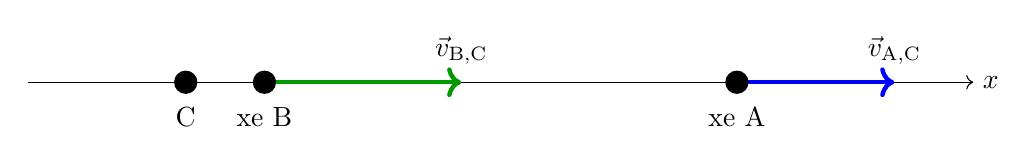
\begin{tikzpicture}
				\coordinate (laxis) at (-2,0);
				\coordinate (C) at (0,0);
				\coordinate (A) at (7,0);
				\coordinate (B) at (1,0);
				\coordinate (va) at ($(A)+(2,0)$);
				\coordinate (vb) at ($(B)+(2.5,0)$);
				\coordinate (raxis) at (10,0);
				\draw[->] (laxis) -- (raxis);
				
				
				\draw[->,ultra thick,blue] (A) -- (va);
				\draw[->,ultra thick,green!60!black] (B) -- (vb);
				\node[below=2mm] at (A) {xe A};
				\node[below=2mm] at (B) {xe B};
				\node[below=2mm] at (C) {C};
				\node[right] at (raxis) {$x$};
				\node[above=1mm] at (va) {$\vec{v}_{\text{A,C}}$};
				\node[above=1mm] at (vb) {$\vec{v}_{\text{B,C}}$};
				\coordinate (va2) at ($(A)-(2,0)$);
				\coordinate (vb2) at ($(B)-(2.5,0)$);
				\filldraw (C) circle (4pt);
				\foreach \i in {B,A}
				{
					\filldraw (\i) circle (4pt);
				}
			\end{tikzpicture}
		\end{center}
		\begin{enumerate}[label=\alph*.]
			\item Vận tốc của ô tô B đối với ô tô A là: 	$$\vec{v}_{\textrm{B,A}}=\vec{v}_{\textrm{B,C}}+\vec{v}_{\textrm{C,A}}==\vec{v}_{\textrm{B,C}}-\vec{v}_{\textrm{A,C}},$$
			Chọn chiều dương là chiều chuyển động của hai ô tô.
			Chiếu lên chiều dương, ta được:
			$$v_{\textrm{B,A}}=v_{\textrm{B,C}}-v_{\textrm{A,C}}= 50\, \textrm{km/h}-40\, \textrm{km/h} = 10\, \textrm{km/h}.$$
			\item Vận tốc của ô tô A đối với ô tô B: 	$$\vec{v}_{\textrm{A,B}}=\vec{v}_{\textrm{A,C}}+\vec{v}_{\textrm{C,B}}=\vec{v}_{\textrm{A,C}}-\vec{v}_{\textrm{B,C}}$$
			Chiếu lên chiều dương, ta được:
			$$v_{\textrm{A,B}}=v_{\textrm{A,C}}-v_{\textrm{B,C}}= 40\, \textrm{km/h}-50\, \textrm{km/h} = -10\, \textrm{km/h}.$$
			
			$\bullet$ \textbf{Lưu ý:} Ta cũng có thể suy ra kết quả này từ kết quả câu \textit{a} bằng:
			$$v_{\textrm{A,B}}=-v_{\textrm{B,A}}=-\SI{10}{\kilo\meter/\hour}.$$
		\end{enumerate}	
	}}

	\viduii{3}{Ô tô A chạy đều trên một đường thẳng với tốc độ $\SI{40}{\kilo\meter/\hour}$. Một ô tô B chạy theo phương vuông góc với ô tô A có tốc độ $\SI{30}{\kilo\meter/\hour}$. Xác định tốc độ của xe ô tô B đối với ô tô A.
	}
	{\hide{
		Ta kí hiệu A là ô tô A, B là ô tô B, C là đất. 
		Vận tốc của ô tô B đối với ô tô A: 	$$\vec{v}_{\textrm{B,A}}=\vec{v}_{\textrm{B,C}}+\vec{v}_{\textrm{C,A}}.$$
		Vectơ $\vec{v}_{\textrm{C,A}}=-\vec{v}_{\textrm{A,C}}$ là vectơ cùng độ lớn nhưng ngược hướng với vectơ $\vec{v}_{\textrm{A,C}}$, được biểu diễn bằng vectơ màu đỏ trong hình. 
		\begin{center}
			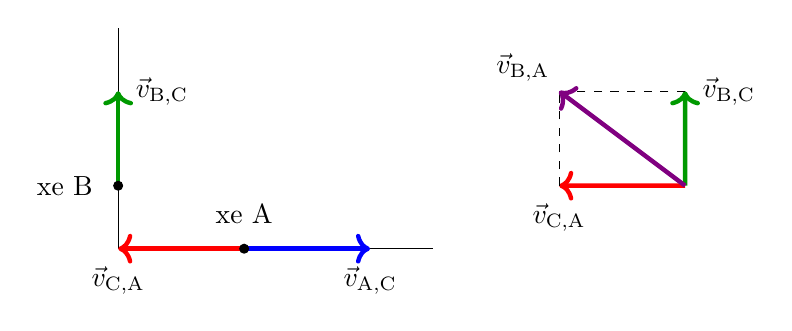
\begin{tikzpicture}[scale=0.8]
				\coordinate (laxis) at (0,0);
				\coordinate (daxis) at (0,0);
				\coordinate (A) at (2,0);
				\coordinate (B) at (0,1);
				\coordinate (va) at ($(A)+(2,0)$);
				\coordinate (vb) at ($(B)+(0,1.5)$);
				\coordinate (raxis) at (5,0);
				\coordinate (uaxis) at (0,3.5);
				\draw[-] (laxis) -- (raxis);
				\draw[-] (daxis) -- (uaxis);
				\draw[->,ultra thick,blue] (A) -- (va);
				\draw[->,ultra thick,green!60!black] (B) -- (vb);
				\node[above=2mm] at (A) {xe A};
				\node[left=2mm] at (B) {xe B};
				%\node[right] at (raxis) {$x$};
				%\node[above] at (uaxis) {$y$};
				\node[below=1mm] at (va) {$\vec{v}_{\text{A,C}}$};
				\node[right=1mm] at (vb) {$\vec{v}_{\text{B,C}}$};
				\coordinate (va2) at ($(A)-(2,0)$);
				\draw[->,ultra thick,red] (A) -- (va2);
				\node[below=1mm] at (va2) {$\vec{v}_{\text{C,A}}$};
				\foreach \i in {B,A}
				{
					\filldraw (\i) circle (2pt);
				}
				\coordinate (O) at (9,1);
				\coordinate (Ou) at ($(O)+(0,1.5)$);
				\coordinate (Ol) at ($(O)-(2,0)$);
				\coordinate (O2) at ($(O)+(-2,1.5)$);
				\draw[->,ultra thick,green!60!black] (O) -- (Ou);
				\draw[->,ultra thick,red] (O) -- (Ol);
				\draw[dashed] (Ou)--(O2);
				\draw[dashed] (Ol)--(O2);
				\draw[->,ultra thick,violet] (O)--(O2);
				\node[below=1mm] at (Ol) {$\vec{v}_{\text{C,A}}$};
				\node[right=1mm] at (Ou) {$\vec{v}_{\text{B,C}}$};
				\node[above left] at (O2) {$\vec{v}_{\text{B,A}}$};
			\end{tikzpicture}
		\end{center}
		
		Do hai ô tô chuyển động theo hai phương vuông góc nhau nên:
		$$v_{\textrm{B,A}}=\sqrt{v_{\textrm{B,C}}^2+v_{\textrm{C,A}}^2}=\sqrt{(\SI{30}{\kilo\meter/\hour})^2+(\SI{40}{\kilo\meter/\hour})^2}=\SI{50}{\kilo\meter/\hour}.$$	
	}}
\end{dang}

\begin{dang}{Áp dụng công thức cộng vận tốc, tính vận tốc tương đối cùng phương, cùng chiều hoặc ngược chiều với vận tốc kéo theo}
	\viduii{3}{Hai bến sông A  và B cách nhau 11,2 km. Một chiếc ca nô phải mất bao nhiêu thời gian để đi từ A đến B rồi trở lại ngay từ B về A. Biết tốc độ của ca nô so với nước không chảy là $v_1=\SI{15}{\kilo\meter/\hour}$ và tốc độ của nước với bờ sông là $v_2=\SI{1}{\kilo\meter/\hour}$.
		
	}
	{\hide{
		Ta gọi $v_{\text{xd}}, v_{\text{nd}}$ lần lượt là tốc độ của thuyền đối với bờ khi nó xuôi dòng và ngược dòng.
		
		Tốc độ của thuyền đối với bờ khi thuyền đi xuôi dòng 
		$$v_{\text{xd}}=v_1+v_2 = \SI{16}{\kilo\meter/\hour}.$$
		Thời gian thuyền đi xuôi dòng khi nó đi từ A đến B
		$$t_{\text{xd}}=\dfrac{AB}{v_{\text{xd}}}=\dfrac{\SI{11.2}{\kilo\meter}}{\SI{16}{\kilo\meter/\hour}}=\SI{0.7}{\hour}.$$
		Tốc độ của thuyền đối với bờ khi thuyền đi ngược dòng 
		$$v_{\text{nd}}=v_1-v_2 = \SI{14}{\kilo\meter/\hour}.$$
		Thời gian thuyền đi ngược dòng khi nó đi từ B đến A
		$$t_{\text{nd}}=\dfrac{AB}{v_{\text{nd}}}=\dfrac{\SI{11.2}{\kilo\meter}}{\SI{14}{\kilo\meter/\hour}}=\SI{0.8}{\hour}.$$
		Tổng thời gian ca nô đi từ A đến B và từ B về A là
		
		$$t= t_{\text{xd}}+ t_{\text{nd}}=\SI{0.7}{\hour}+\SI{0.8}{\hour}=\SI{1.5}{\hour}.$$
	}}

	\viduii{3}{Một chiếc thuyền chạy xuôi dòng sông mất 2 giờ để chạy thẳng đều từ bến A ở thượng lưu tới bến B ở hạ lưu và phải mất 3 giờ khi chạy ngược lại từ bến B về đến bến A. Cho rằng tốc độ của thuyền đối với nước là $v_1=\SI{30}{\kilo\meter/\hour}$, tốc độ của dòng nước đối với bờ sông là $v_2$. Tính khoảng cách AB và $v_2$.
	}
	{\hide{
		Ta gọi $v_{\text{xd}}, v_{\text{nd}}$ lần lượt là tốc độ của thuyền khi xuôi dòng và ngược dòng.
		
		Tốc độ của thuyền đối với bờ khi thuyền đi xuôi dòng là:
		$$v_{\text{xd}}=v_1+v_2.$$
		Thời gian thuyền đi xuôi dòng khi nó đi từ A đến B:
		\begin{equation*}
			t_{\text{xd}}=\dfrac{AB}{v_{\text{xd}}}= \dfrac{AB}{v_1+v_2}\quad \Rightarrow\quad \text{AB}=(v_1+v_2)t_{\text{xd}}
		\end{equation*}
		Tốc độ của thuyền đối với bờ khi thuyền đi ngược dòng là:
		$$v_{\text{nd}}=v_1-v_2.$$
		Thời gian thuyền đi ngược dòng khi nó đi từ B đến A:
		\begin{equation*}
			t_{\text{nd}}=\dfrac{AB}{v_{\text{nd}}}= \dfrac{AB}{v_1-v_2}\quad\Rightarrow\quad \text{AB}=(v_1-v_2)t_\text{nd}.
		\end{equation*}
		Từ hai phương trình trên, ta suy ra tốc độ dòng nước và khoảng cách AB:
		\begin{eqnarray*}
			(v_1+v_2)t_{\text{xd}}&=&(v_1-v_2)t_{\text{nd}}\\
			\quad\Rightarrow\quad	v_2&=&\left(\dfrac{t_\text{nd}-t_\text{xd}}{t_{\text{xd}}+t_\text{nd}}\right)\cdot v_1\\
			&=&\left(\dfrac{\SI{3}{\hour}-\SI{2}{\hour}}{\SI{2}{\hour}+\SI{3}{\hour}}\right)\times\SI{30}{\kilo\meter/\hour}\\
			&=&\SI{6}{\kilo\meter/\hour},\\
			\quad\Rightarrow\quad \text{AB}&=&(v_1+v_2)t_\text{xd}\\
			&=&(\SI{30}{\kilo\meter/\hour}+\SI{6}{\kilo\meter/\hour})\times\SI{2}{\hour}\\
			&=&\SI{72}{\kilo\meter}.
		\end{eqnarray*}
	}}
\end{dang}
%				\let\lesson\undefined
\newcommand{\lesson}{\phantomlesson{Bài 5.}}
\setcounter{section}{2}
\section{Bài tập trắc nghiệm}
\begin{enumerate}[label=\bfseries Câu \arabic*:,leftmargin=1.5cm]
	\item \mkstar{2}\\
	{Một hành khách ngồi trong xe A, nhìn qua cửa sổ thấy xe B bên cạnh và sân ga đều chuyển động như nhau. Như vậy
	\begin{mcq}(2)
		\item xe A đứng yên, xe B chuyển động.
		\item xe A chạy, xe B đứng yên.
		\item xe A và xe B chạy cùng chiều.
		\item xe A và xe B chạy ngược chiều.
	\end{mcq}
}
\hideall{
\textbf{Đáp án: B.}
}

\item \mkstar{2}\\
{Chọn phát biểu \textbf{sai}:
\begin{mcq}
	\item Vận tốc của chất điểm phụ thuộc vào hệ qui chiếu.
	\item Trong các hệ qui chiếu khác nhau thì vị trí của cùng một vật là khác nhau.
	\item Khoảng cách giữa hai điểm trong không gian là tương đối.
	\item Tọa độ của một chất điểm phụ thuộc hệ qui chiếu.
\end{mcq}
}
\hideall{
\textbf{Đáp án: C.}\\
Khoảng cách giữa hai điểm trong không gian không phụ thuộc vào hệ quy chiếu.
}

\item \mkstar{2}\\
{Chọn câu đúng, đứng ở Trái Đất ta sẽ thấy:
\begin{mcq}
	\item Trái Đất đứng yên, Mặt Trời và Mặt Trăng quay quanh Trái Đất.
	\item Mặt Trời đứng yên, Trái Đất quay quanh Mặt Trời, Mặt trăng quay quanh Trái đất.
	\item Mặt Trời đứng yên, Trái Đất và Mặt Trăng quay quanh Mặt Trời.
	\item Mặt Trời và mặt đất đứng yên, Mặt Trăng quay quanh Trái Đất.
\end{mcq}
}
\hideall{
\textbf{Đáp án: A.}
}

\item \mkstar{2}\\
{Một hành khách ngồi trong toa tàu H, nhìn qua cửa sổ thấy toa tàu N bên cạnh và gạch lát sân ga đều chuyển động như nhau. Hỏi toa tàu nào chạy?
\begin{mcq}(2)
	\item Tàu N chạy tàu H đứng yên.
	\item Cả 2 tàu đều chạy.
	\item Tàu H chạy tàu N đứng yên.
	\item Cả 2 tàu đều đứng yên.
\end{mcq}
}
\hideall{
\textbf{Đáp án: C.}
}

\item \mkstar{2}\\
{Biết vận tốc của ca nô so với mặt nước đứng yên là $\SI{10}{\meter/\second}$. Vận tốc của dòng nước là $\SI{4}{\meter/\second}$. Tính vận tốc của ca nô khi
\begin{enumerate}[label=\alph*)]
	\item ca nô đi xuôi dòng.
	\begin{mcq}(4)
		\item $\SI{14}{\meter/\second}$.
		\item $\SI{9}{\meter/\second}$.
		\item $\SI{6}{\meter/\second}$.
		\item $\SI{5}{\meter/\second}$.
	\end{mcq}
\item ca nô đi ngược dòng.
\begin{mcq}(4)
	\item $\SI{14}{\meter/\second}$.
	\item $\SI{9}{\meter/\second}$.
	\item $\SI{6}{\meter/\second}$.
	\item $\SI{5}{\meter/\second}$.
\end{mcq}
\end{enumerate}

}
\hideall{
\textbf{Đáp án: A - C.}
}

\item  \mkstar{3}\\
{Hai ô tô A và B chạy cùng chiều trên cùng một đoạn đường với vận tốc $\SI{70}{\kilo\meter/\hour}$ và $\SI{65}{\kilo\meter/\hour}$. Vận tốc của ô tô A so với ô tô B bằng
	\begin{mcq}(4)
		\item $\SI{30}{\kilo\meter/\hour}$.
		\item $\SI{5}{\kilo\meter/\hour}$.
		\item $\SI{135}{\kilo\meter/\hour}$.
		\item $\SI{65}{\kilo\meter/\hour}$.
	\end{mcq}

}
\hideall{
\textbf{Đáp án: B.}
}

\item \mkstar{3}\\
{A ngồi trên một toa tàu chuyển động với vận tốc $\SI{15}{\kilo\meter/\hour}$ đang rời ga. B ngồi trên một toa tàu khác chuyển động với vận tốc $\SI{10}{\kilo\meter/\hour}$ đang đi ngược chiều vào ga. Hai đường tàu song song với nhau. Chọn chiều dương là chiều chuyển động của đoàn tàu mà A ngồi. Tính vận tốc của B đối với A.
	\begin{mcq}(4)
		\item $\SI{-5}{\kilo\meter/\hour}$.
		\item $\SI{5}{\kilo\meter/\hour}$.
		\item $\SI{25}{\kilo\meter/\hour}$.
		\item $\SI{-25}{\kilo\meter/\hour}$.
	\end{mcq}

}
\hideall{
\textbf{Đáp án: D.}\\
Chọn chiều dương là chiều chuyển động của tàu A.

$\overrightarrow{v_\text{AD}}$ là vận tốc của tàu A đối với đất;

$\overrightarrow{v_\text{BD}}$ là vận tốc của tàu B đối với đất;

$\overrightarrow{v_\text{BA}}$ là vận tốc của tàu B đối với tàu A.

Theo công thức cộng vận tốc:
$$\overrightarrow{v_\text{BD}} = \overrightarrow{v_\text{BA}}+\overrightarrow{v_\text{AD}} \Rightarrow \overrightarrow{v_\text{BA}} = \overrightarrow{v_\text{BD}} - \overrightarrow{v_\text{AD}}=\overrightarrow{v_\text{BD}} + \overrightarrow{-v_\text{AD}}$$

Chiếu lên chiều chuyển động của tàu A:
$$v_\text{AB} = -v_\text{BD} - v_\text{AD} = -10-15 = \SI{-25}{km/h}$$

Vận tốc của tàu B đối với tàu A có độ lớn $\SI{25}{km/h}$ và ngược chiều so với chiều chuyển động của tàu A.
}

\item \mkstar{3}\\
{Hai bến sông A và B cùng nằm trên một bờ sông, cách nhau $\SI{18}{\kilo\meter}$. Cho biết độ lớn vận tốc của ca nô đối với nước là $u =\SI{16.2}{\kilo\meter/\hour}$ và độ lớn vận tốc của nước đối với bờ sông là $v=\SI{5.4}{\kilo\meter/\hour}$. Thời gian để ca nô chạy xuôi dòng từ A đến B rồi lại chạy ngược dòng trở về A là
\begin{mcq}(4)
	\item 1 giờ 40 phút.
	\item 1 giờ 20 phút.
	\item 2 giờ 30 phút.
	\item 2 giờ 10 phút.
\end{mcq}
}
\hideall{
\textbf{Đáp án: C.}\\
Thời gian ca nô chạy xuôi dòng từ A đến B rồi chạy ngược lại trở về A:
$$t=\dfrac{s}{u+v}+\dfrac{s}{u-v}=\SI{2.5}{\second}.$$
}

\item \mkstar{3}\\
{Ô tô A chạy thẳng về hướng Tây với độ lớn vận tốc $\SI{40}{\kilo\meter/\hour}$. Ô tô B chạy thẳng về hướng Bắc với độ lớn vận tốc $\SI{60}{\kilo\meter/\hour}$. Độ lớn vận tốc của ô tô B so với người ngồi trên ô tô A gần giá trị nào nhất sau đây?
\begin{mcq}(4)
	\item $\SI{85}{\kilo\meter/\hour}$.
	\item $\SI{90}{\kilo\meter/\hour}$.
	\item $\SI{65}{\kilo\meter/\hour}$.
	\item $\SI{75}{\kilo\meter/\hour}$.
\end{mcq}
}
\hideall{
\textbf{Đáp án: D.}\\
Vận tốc của ô tô B đới với người ngồi trên ô tô A:
$$\overrightarrow{v_{BA}}=\overrightarrow{v_{BD}}-\overrightarrow{v_{AD}}$$
Vì $\overrightarrow{v_{BD}}\bot \overrightarrow{v_{AD}}$ nên
$$v_{BA}=\sqrt{v^2_{BD}+v^2_{AD}}\approx\SI{72}{\kilo\meter/\hour}$$
}

\item \mkstar{4}\\
{Một người lái xuồng máy cho xuồng chạy ngang con sông rộng $\SI{240}{\meter}$. Mũi xuồng luôn luôn vuông góc với bờ sông, nhưng do nước chảy nên xuồng sang đến bờ bên kia tại một điểm cách bến dự định $\SI{180}{\meter}$ về phía hạ lưu và xuồng đi hết 1 phút. Độ lớn vận tốc của xuồng so với bờ là
\begin{mcq}(4)
	\item $\SI{8}{\meter/\second}$.
	\item $\SI{9}{\meter/\second}$.
	\item $\SI{6}{\meter/\second}$.
	\item $\SI{5}{\meter/\second}$.
\end{mcq}
}
\hideall{
\textbf{Đáp án: D.}\\
Độ dịch chuyển của xuồng so với vị trí ban đầu:
$$d=\sqrt{240^2+180^2}=\SI{300}{\meter}$$
Độ lớn vận tốc của xuồng so với bờ:
$$v_{xd}=\dfrac{d}{t}=\SI{5}{\meter/\second}.$$
}
\end{enumerate}
\section{Bài tập tự luận}
\begin{enumerate}[label=\bfseries Bài \arabic*:,leftmargin=1.5cm]
	\item \mkstar{3}\\
	{Biết $\overrightarrow{d_1}$ là độ dịch chuyển $\SI{10}{\meter}$ về phía đông còn $\overrightarrow{d_2}$ là độ dịch chuyển $\SI{6}{\meter}$ về phía tây. Hãy xác định độ dịch chuyển tổng hợp trong 2 trường hợp sau
		\begin{enumerate}[label=\alph*)]
			\item $\overrightarrow{d}=\overrightarrow{d_1}+\overrightarrow{d_2}$.
			\item $\overrightarrow{d}=\overrightarrow{d_1}+3\overrightarrow{d_2}$.
		\end{enumerate}
		
	}
	\hideall{
		\begin{enumerate}[label=\alph*)]
			\item $d=\SI{4}{\meter}$ về hướng đông.
			\item $d=\SI{8}{\meter}$ về hướng tây
		\end{enumerate}
	}

	\item \mkstar{3}
	
	{Một ô tô A chạy đều trên một đường thẳng với vận tốc $\SI{40}{km/h}$. Một ô tô B đuổi theo ô tô A với vận tốc $\SI{60}{km/h}$. Xác định vận tốc của ô tô B đối với ô tô A và của ô tô A đối với ô tô B.}
	\hideall{
		Chọn chiều dương là chiều chuyển động của hai xe.
		
		$\overrightarrow{v_\text{AD}}$ là vận tốc của xe A đối với đất;
		
		$\overrightarrow{v_\text{BD}}$ là vận tốc của xe B đối với đất;
		
		$\overrightarrow{v_\text{BA}}$ là vận tốc của xe B đối với xe A.
		
		Theo công thức cộng vận tốc:
		$$\overrightarrow{v_\text{AB}} = \overrightarrow{v_\text{AD}}+\overrightarrow{v_\text{DB}} \Rightarrow \overrightarrow{v_\text{AB}} = \overrightarrow{v_\text{AD}} - \overrightarrow{v_\text{BD}}$$
		
		Chiếu lên hướng chuyển đông của ô tô A:
		$$v_\text{AB} = 40-60=-20\ \text{km/h}$$
		
		Vậy $v_\text{BA} = 20\ \text{km/h}$.
	}
	
	\item \mkstar{3}
	
	
	{   
		Trên đoàn tàu đang chạy thẳng với vận tốc trung bình $\SI{36}{km/h}$ so với mặt đường. Hãy xác định vận tốc của hành khách đối với mặt đường nếu người này chuyển động về cuối đoàn tàu với vận tốc có cùng độ lớn $\SI{1}{m/s}$.
	}
	\hideall
	{
		
		Đổi: $\SI{36}{km/h} = \SI{10}{m/s}$.
		
		Gọi:
		
		$\vec v_{1,2}$ là vận tốc của hành khách so với tàu.
		
		$\vec v_{2,3}$ là vận tốc của tàu so với mặt đường.
		
		$\vec v_{1,3}$ là vận tốc của hành khách so với mặt đường.
		
		Ta có:
		
		$$\vec v_{1,3} = \vec v_{1,2} + \vec v_{2,3}.$$
		
		Chọn chiều chuyển động của tàu đối với đất làm chiều dương:
		
		$$v_{1,3} = - v_{1,2} + v_{2,3} = \SI{9}{m/s}.$$
		
		
	}

	\item \mkstar{3}
	
	
	{
		Trên đoàn tàu đang chạy thẳng với vận tốc trung bình $\SI{36}{km/h}$ so với mặt đường, một hành khách đi về đầu tàu với vận tốc $\SI{1}{m/s}$ so với mặt sàn tàu.
		\begin{center}
			\includegraphics[scale=1]{../figs/VN10-2022-PH-TP005-3.jpg}
		\end{center}
		\begin{enumerate}[label=\alph*)]
			\item Hành khách này tham gia mấy chuyển động?
			\item Làm cách nào để xác định được vận tốc của hành khách đối với mặt đường?
		\end{enumerate}
	}
	\hideall
	{
		\begin{enumerate}[label=\alph*)]
			\item Hành khách này tham gia 2 chuyển động: Chuyển động với vận tốc $\SI{1}{m/s}$ so với sàn tàu và chuyển động do tàu kéo đi với vận tốc bằng vận tốc của tàu so với mặt đường. Chuyển động của hành khách so với mặt đường là tổng hợp của hai chuyển động trên.
			\item Gọi:
			
			- $\vec v_{1,2}$ là vận tốc của hành khách so với tàu.
			
			- $\vec v_{2,3}$ là vận tốc của tàu so với mặt đường.
			
			- $\vec v_{1,3}$ là vận tốc của hành khách so với mặt đường.
			
			Thì:
			
			$$\vec v_{1,3} = \vec v_{1,2} + \vec v_{2,3}$$
			
			Chọn chiều chuyển động của tàu làm chiều dương:
			
			$$v_{1,3} = v_{1,2} + v_{2,3} = \SI{11}{m/s}.$$
			
			Hướng của vận tốc người so với mặt đường là hướng đoàn tàu chạy.
		\end{enumerate}
	}

	\item \mkstar{3}
	
	
	{
		Một người bơi trong bể bơi yên lặng có thể đạt tới vận tốc $\SI{1}{m/s}$. Nếu người này bơi xuôi dòng sông có dòng chảy với vận tốc $\SI{1}{m/s}$ thì có thể đạt vận tốc tối đa là bao nhiêu?
	}
	\hideall
	{
		Gọi:
		
		$\vec v_{1,2}$ là vận tốc của người so với nước.
		
		$\vec v_{2,3}$ là vận tốc của nước so với bờ.
		
		$\vec v_{1,3}$ là vận tốc của người so với bờ.
		
		Ta có:
		
		$$\vec v_{1,3} = \vec v_{1,2} + \vec v_{2,3}.$$
		
		- Khi người bơi trong bể nước yên lặng, thì $v_{2,3} = 0$:
		
		$$v_{1,2} = v_{1,3} = \SI{1}{m/s}.$$
		
		- Khi người này bơi xuôi dòng chảy với vận tốc $v_{2,3} = \SI{1}{m/s}$:
		
		
		$$v_{1,3} = v_{1,2} + v_{2,3} = \SI{2}{m/s}.$$
		
		Vậy nếu người này bơi xuôi dòng sông có dòng chảy với vận tốc $\SI{1}{m/s}$ thì có thể đạt vận tốc tối đa là $\SI{2}{m/s}.$
		
		
	}
	\item \mkstar{3}
	
	
	{
		Một ca nô chạy hết tốc lực trên mặt nước yên lặng có thể đạt $\SI{21,5}{km/h}$. Ca nô này chạy xuôi dòng sông trong 1 giờ rồi quay lại thì phải mất 2 giờ nữa mới về tới vị trí ban đầu. Hãy tính vận tốc chảy của dòng sông.
	}
	\hideall
	{
		Gọi:
		
		$\vec v_{1,2}$ là vận tốc của canô so với nước.
		
		
		$\vec v_{2,3}$ là vận tốc của nước so với bờ.
		
		
		$\vec v_{1,3}$ là vận tốc của canô so với bờ.
		
		Ta có:
		
		$$\vec v_{1,3} = \vec v_{1,2} + \vec v_{2,3}.$$
		
		- Khi canô chạy trên mặt nước yên lặng, tức $v_{2,3} = 0$:
		
		
		$$v_{1,2} = v_{1,3} = \SI{21,5}{km/h}.$$
		
		- Khi canô chạy xuôi dòng sông, ta có:
		
		$$v_{1,3} = v_{1,2} + v_{2,3} =\dfrac{d}{t_1}$$
		
		- Khi canô quay lại, ta có:
		
		$$v'_{1,3} = v_{1,2} - v_{2,3} =\dfrac{d}{t_2}$$
		
		Thay các đại lượng của đề vào (1) và (2) ta suy ra:
		
		$$\begin{cases}
			d = \SI{28,67}{km}.\\
			v_{2,3} = \SI{7,17}{km/h}.
		\end{cases}$$
		
		Vậy vận tốc chảy của dòng sông là $\SI{7,17}{km/h}$.
		
		
	}
	\item \mkstar{3}
	
	
	{
		Một ca nô chạy trong hồ nước yên lặng có vận tốc tối đa $\SI{18}{km/h}$. Nếu ca nô chạy ngang một con sông có dòng chảy theo hướng Bắc - Nam với vận tốc lên tới $\SI{5}{m/s}$ thì vận tốc tối đa nó có thể đạt được so với bờ sông là bao nhiêu và theo hướng nào?
	}
	\hideall
	{
		\begin{center}
			\includegraphics[scale=1]{../figs/VN10-2022-PH-TP005-4.jpg}
		\end{center}
		Gọi vận tốc của ca nô đối với mặt nước là $\vec v_{1,2}$; 
		
		Vận tốc của nước chảy đối với bờ sông là $\vec v_{2,3}$. 
		
		Vận tốc của ca nô đối với bờ sông:
		
		$$\vec v_{1,3} = \vec v_{1,2} + \vec v_{2,3}.$$
		
		Suy ra:
		
		$$v_{1,3} = \sqrt{ v_{1,2}^2 + v_{2,3}^2} = \SI{7,07}{m/s}.$$
		
		Vì $\text{AB} = \text{BC}$ nên tam giác ABC là tam giác vuông cân và góc A bằng $45^\circ$. Hướng của vận tốc nghiêng $45^\circ$ theo hướng Đông - Nam.
	}
	\item \mkstar{3}
	
	
	{
		Một máy bay đang bay theo hướng Bắc với vận tốc $\SI{200}{m/s}$ thì bị gió từ hướng Tây thổi vào với vận tốc $\SI{20}{m/s}$. Xác định vận tốc tổng hợp của máy bay lúc này.
	}
	\hideall
	{
		Gọi:
		
		$\vec v_{1,2}$ là vận tốc của máy bay so với gió.
		
		$\vec v_{2,3}$ là vận tốc của gió so với đường bay.
		
		$\vec v_{1,3}$ là vận tốc của máy bay so với đường bay.
		
		Ta có:
		
		$$\vec v_{1,3} = \vec v_{1,2} + \vec v_{2,3}.$$
		
		Vận tốc tổng hợp của máy bay lúc này là
		
		$$v_{1,3} = \sqrt{v_{1,2}^2 + v^2_{2,3}} = \SI{201}{m/s}.$$
		Vận tốc tổng hợp hướng theo hướng Tây - Bắc hợp với hướng Nam - Bắc 1 góc 
		$$\tan\alpha=\dfrac{v_{23}}{v_{12}}=\dfrac{1}{10}\Rightarrow \alpha =\SI{5.7}{\degree}.$$
	}
		

\item \mkstar{3}\\
{Một người bơi từ bờ này sang bờ kia của một con sông rộng $\SI{50}{\meter}$ theo hướng vuông góc với bờ sông. Do nước sông chảy mạnh nên quãng đường người đó bơi gấp 2 lần so với khi bơi trong bể bơi.
	\begin{enumerate}[label=\alph*)]
		\item Hãy xác định độ dịch chuyển của người này khi bơi sang bờ sông bên kia.
		\item Vị trí điểm tới cách điểm đối diện với điểm khởi hành của người bơi là bao nhiêu mét?
	\end{enumerate}
	
}
\hideall{
	\begin{center}
		\includegraphics[width=0.15\linewidth]{../figs/VN10-2023-PH-TP0002-6}
	\end{center}
	\begin{enumerate}[label=\alph*)]
		\item $d=\SI{100}{\meter}$ theo hướng làm với bờ sông một góc $\alpha=\SI{30}{\degree}$.
		\item $AB=OA\tan\SI{60}{\degree}=\SI{86.6}{\meter}$.
	\end{enumerate}
}

\item \mkstar{3}\\
{Một người chèo thuyền qua một con sông rộng $\SI{400}{\meter}$. Muốn cho thuyền đi theo đường AB thì người đó phải luôn hướng mũi thuyền theo hướng AC. Biết thuyền qua sông hết $\SI{8}{\minute} \SI{20}{\second}$ và tốc độ của dòng nước là $\SI{0.6}{\meter/\second}$. Tìm tốc độ của thuyền so với dòng nước.
	\begin{center}
		\includegraphics[width=0.35\linewidth]{../figs/VN10-2023-PH-TP0002-7}
	\end{center}
	
}
\hideall{
	Quãng đường nước đẩy thuyền trôi:
	$$BC=v_n\cdot t=\SI{300}{\meter}$$
	Tốc độ của thuyền so với dòng nước:
	$$v_\text{thuyền/nước}=\dfrac{AC}{t}=\dfrac{\sqrt{AB^2+BC^2}}{t}=\SI{1}{\meter/\second}.$$
}

\end{enumerate}

%			\stopMyChapterToc
%		\mychapter[Ôn tập chương 2]{Ôn tập chương 2}
%			\startMyChapterToc	
%				\let\lesson\undefined
\newcommand{\lesson}{\phantomlesson{Bài 3.}}


\setcounter{section}{0}
\section{Bài tập trắc nghiệm}
\begin{enumerate}[label=\bfseries Câu \arabic*:,leftmargin=1.5cm]
	
% 2222222222222222222222222
	\item \mkstar{1}\\
	{Tốc độ là đại lượng đặc trưng cho
		\begin{mcq}(2)
			\item tính chất nhanh hay chậm của chuyển động.
			\item sự thay đổi hướng của chuyển động.
			\item khả năng duy trì chuyển động của vật.
			\item sự thay đổi vị trí của vật trong không gian.
		\end{mcq}
}
\hideall{
\textbf{Đáp án: A.}
}

\item \mkstar{2}\\
{Đồ thị vận tốc - thời gian của chuyển động thẳng đều là một đường thẳng
	\begin{mcq}(2)
		\item đi qua gốc toạ độ.
		\item song song với trục hoành.
		\item bất kì.
		\item song song với trục tung.
	\end{mcq}

}
\hideall{
\textbf{Đáp án: B.}
}


\item \mkstar{2}\\
{Chọn phát biểu đúng
	\begin{mcq}
		\item Vectơ độ dịch chuyển thay đổi phương liên tục khi vật chuyển động.
		\item Vectơ độ dịch chuyển có độ lớn luôn bằng quãng đường đi được của chất điểm.
		\item Khi vật chuyển động thẳng không đổi chiều, độ lớn của vectơ độ dịch chuyển bằng quãng đường đi được.
		\item Vận tốc tức thời cho ta biết chiều chuyển động nên luôn có giá trị dương.
	\end{mcq}

}
\hideall{
\textbf{Đáp án: C.}
}


\item \mkstar{2}\\
{Chỉ ra phát biểu sai.
	\begin{mcq}
		\item Vectơ độ dịch chuyển là một vectơ nối vị trí đầu và vị trí cuối của vật chuyển động.
		\item Vectơ độ dịch chuyển có độ lớn luôn bằng quãng đường đi được của vật.
		\item Khi vật đi từ điểm A đến điểm B, sau đó đến điểm C, rồi quay về A thì độ dịch chuyển của vật có độ lớn bằng 0.
		\item Độ dịch chuyển có thể có giá trị âm, dương hoặc bằng không.
	\end{mcq}

}
\hideall{
\textbf{Đáp án: B.}
}

\item \mkstar{2}\\
{Chuyển động nào sau đây là chuyển động thẳng nhanh dần?
	\begin{mcq}(2)
		\item Chuyển động của ô tô khi bắt đầu chuyển động.
		\item Chuyển động của xe buýt khi vào trạm.
		\item Chuyển động của xe máy khi tắc đường.
		\item Chuyển động của đầu kim đồng hồ.
	\end{mcq}

}
\hideall{
\textbf{Đáp án: A.}
}


\item \mkstar{2}\\
{Một người chuyển động thẳng có độ dịch chuyển $d_1$ tại thời điểm $t_1$ và độ dịch chuyển $d_2$ tại thời điểm $t_2$. Vận tốc trung bình của vật trong khoảng thời gian từ $t_1$ đến $t_2$ là
	\begin{mcq}(4)
		\item $v_{tb}=\dfrac{d_1-d_2}{t_1+t_2}$.
		\item $v_{tb}=\dfrac{d_2-d_1}{t_2-t_1}$.
		\item $v_{tb}=\dfrac{d_1+d_2}{t_2-t_1}$.
		\item $v_{tb}=\dfrac{1}{2}\left(\dfrac{d_1}{t_1}+\dfrac{d_2}{t_2}\right)$.
	\end{mcq}

}
\hideall{
\textbf{Đáp án: B.}
}

\item \mkstar{2}\\
{Tính chất nào sau đây là của vận tốc, không phải là của tốc độ của một chuyển động?
	\begin{mcq}
		\item Đặc trưng cho sự nhanh chậm của chuyển động.
		\item Có đơn vị là $\si{\kilo\meter/\hour}$.
		\item Không thể có độ lớn bằng 0.
		\item Có phương xác định.
	\end{mcq}

}
\hideall{
\textbf{Đáp án: D.}
}

\item \mkstar{2}\\
{Cho đồ thị độ dịch chuyển - thời gian của một vật như hình \ref{fig:0002-1}. Trong những khoảng thời gian nào thì vật chuyển động thẳng đều?
	\begin{center}
		\includegraphics[width=0.3\linewidth]{../figs/VN10-2023-PH-TP0002-1}
		\captionof{figure}{}
		\label{fig:0002-1}
	\end{center}
	\begin{mcq}
		\item Trong khoảng thời gian từ 0 đến $t_1$ và từ $t_1$ đến $t_2$.
		\item Trogn khoảng thời gian từ $t_1$ đến $t_2$.
		\item Trong khoảng thời gian từ $0$ đến $t_3$.
		\item Trong khoảng thời gian từ 0 đến $t_1$ và từ $t_2$ đến $t_3$.
	\end{mcq}

}
\hideall{
\textbf{Đáp án: D.}
}

\item \mkstar{2}\\
{Cặp đồ thị nào dưới đây là của chuyển động thẳng đều?
	\begin{center}
		\includegraphics[width=0.7\linewidth]{../figs/VN10-2023-PH-TP0002-9}
	\end{center}
\begin{mcq}(4)
	\item I và III.
	\item I và IV.
	\item II và III.
	\item II và IV.
\end{mcq}
}
\hideall{
\textbf{Đáp án: B.}
}

\item \mkstar{2}\\
{Hình bên là đồ thị độ dịch chuyển - thời gian của ô tô chuyển động thẳng theo một hướng xác định. Ô tô đi với tốc độ lớn nhất trong đoạn đường nào?
	\begin{center}
		\includegraphics[width=0.3\linewidth]{../figs/VN10-2023-PH-TP0002-11}
	\end{center}
	\begin{mcq}(4)
		\item 1.
		\item 2.
		\item 3.
		\item 4.
	\end{mcq}

}
\hideall{
\textbf{Đáp án: B.}
}
\item \mkstar{2}


{Tàu Thống Nhất TN1 đi từ ga Huế vào ga Sài Gòn mất $\SI{20}{h}$. Biết tốc độ trung bình của tàu là $\SI{15}{m/s}$. Hỏi chiều dài của đường ray từ Huế vào Sài Gòn?
	\begin{mcq}(4)
		\item $\SI{3000}{km}$. 
		\item $\SI{1080}{km}$.
		\item $\SI{1000}{km}$.
		\item $\SI{1333}{km}$.
	\end{mcq}
}

\hideall
{		\textbf{Đáp án: B.}
	
	Chiều dài của đường ray từ Huế vào Sài Gòn:
	$$s=vt=\SI{1080}{km}$$
	
}
\item \mkstar{2}


{Trong trận đấu giữa Đức và Áo ở EURO 2008, tiền vệ Michael Ballack của đội tuyển Đức sút phạt cách khung thành của đội Áo $\SI{30}{m}$. Các chuyên gia tính được tốc độ trung bình của quả phạt đó lên tới $\SI{108}{km/h}$. Hỏi thời gian bay của quả bóng là bao nhiêu?
	\begin{mcq}(4)
		\item $\SI{1}{s}$. 
		\item $\SI{36}{s}$. 
		\item $\SI{1.5}{s}$.  
		\item $\SI{3.6}{s}$. 
	\end{mcq}
}

\hideall
{\textbf{Đáp án: A.}
	
	Thời gian bay của quả bóng:
	$$t=\dfrac{s}{v} = 1\ \text s$$
	
}
\item \mkstar{2}


{Hưng đạp xe lên dốc dài $\SI{100}{m}$ với vận tốc 2 m/s, sau đó xuống dốc dài $\SI{140}{m}$ hết 30 s. Hỏi tốc độ trung bình của Hưng trên cả hai đoạn đường?
	\begin{mcq}(4)
		\item $\SI{50}{m/s}$. 
		\item $\SI{8}{m/s}$. 
		\item $\SI{4.67}{m/s}$. 
		\item $\SI{3}{m/s}$.
	\end{mcq}
}

\hideall
{\textbf{Đáp án: D.}
	
	Thời gian trên đoạn đường thứ nhất:
	$$t_1=\dfrac{s_1}{v_1} = 50\ \text s$$
	
	Tốc độ trung bình trên cả hai đoạn đường:
	$$v=\dfrac{s_1+s_2}{t_1+t_2} = 3\ \text {m/s}$$
	
}

% 333333333333333333333333333333333333333

\item \mkstar{3}\\
{Đồ thị toạ độ - thời gian của hai xe 1 và 2 được biểu diễn như hình \ref{fig:0002-2}. Hai xe gặp nhau tại vị trí cách vị trí xuất phát của 2 xe một khoảng
	\begin{center}
		\includegraphics[width=0.3\linewidth]{../figs/VN10-2023-PH-TP0002-2}
		\captionof{figure}{}
		\label{fig:0002-2}
	\end{center}
	\begin{mcq}(4)
		\item $\SI{40}{\kilo\meter}$.
		\item $\SI{30}{\kilo\meter}$.
		\item $\SI{35}{\kilo\meter}$.
		\item $\SI{70}{\kilo\meter}$.
	\end{mcq}

}
\hideall{
\textbf{Đáp án: A.}
}


\item \mkstar{3}\\
{Phương trình chuyển động và độ lớn vận tốc của hai chuyển động có đồ thị như hình bên là
	\begin{center}
		\includegraphics[width=0.3\linewidth]{../figs/VN10-2023-PH-TP0002-10}
	\end{center}
\begin{mcq}(2)
	\item $d_1=\xsi{60-10t}{\kilo\meter}; v_1=\SI{10}{\kilo\meter/\hour}$\\
		$d_2=\xsi{12t}{\kilo\meter}; v_2=\SI{12}{\kilo\meter/\hour}$.
	\item $d_1=\xsi{60+10t}{\kilo\meter}; v_1=\SI{10}{\kilo\meter/\hour}$\\
		$d_2=\xsi{-10t}{\kilo\meter}; v_2=\SI{10}{\kilo\meter/\hour}$.
	\item $d_1=\xsi{60-20t}{\kilo\meter}; v_1=\SI{20}{\kilo\meter/\hour}$\\
		$d_2=\xsi{12t}{\kilo\meter}; v_2=\SI{12}{\kilo\meter/\hour}$.
	\item $d_1=\xsi{-10t}{\kilo\meter}; v_1=\SI{10}{\kilo\meter/\hour}$\\
		$d_2=\xsi{12t}{\kilo\meter}; v_2=\SI{12}{\kilo\meter/\hour}$.
\end{mcq}
}
\hideall{
\textbf{Đáp án: A.}\\
Độ lớn vận tốc của mỗi xe
\begin{align*}
	\begin{cases}
		\left|v_1\right|=\dfrac{\left|0-60\right|}{6}=\SI{10}{\kilo\meter/\hour}\\
		\left|v_2\right|=\dfrac{\left|60-0\right|}{5}=\SI{12}{\kilo\meter/\hour}
	\end{cases}
\end{align*}
Phương trình chuyển động của hai xe:
\begin{align*}
	\begin{cases}
		d_1=60-10t\qquad\left(\si{\kilo\meter}\right)\\
		d_2=12t\qquad\left(\si{\kilo\meter}\right)
	\end{cases}
\end{align*}
}

\item \mkstar{3}\\
{Hãy thiết lập phương trình chuyển động của một ô tô chuyển động thẳng đều biết. Ô tô chuyển động theo chiều dương với vận tốc $\SI{10}{\meter/\second}$ và ở thời điểm $\SI{3}{\second}$ thì vật có tọa độ $\SI{60}{\meter}$.
	\begin{mcq}(4)
		\item $\xsi{30+10t}{\meter}$.
		\item $\xsi{20+10t}{\meter}$.
		\item $\xsi{10+20t}{\meter}$.
		\item $\xsi{40+10t}{\meter}$.
	\end{mcq}

}
\hideall{
\textbf{Đáp án: A.}\\
Phương trình chuyển động của ô tô:
$$x=x_0+10t$$
Khi $t=\SI{3}{\second}$ thì vật có toạ độ $x=\SI{60}{\meter}\Rightarrow x_0=\SI{30}{\meter}.$
}

\item \mkstar{3}\\
{Lúc 7 giờ sáng, tại A xe thứ nhất chuyển động thẳng đều với tốc độ $\SI{12}{\kilo\meter/\hour}$ để về B. Một giờ sau, tại B xe thứ hai cũng chuyển động thẳng đều với tốc độ $\SI{48}{\kilo\meter/\hour}$ theo chiều ngược lại để về A. Cho đoạn thẳng $AB=\SI{72}{\kilo\meter}$. Khoảng cách giữa hai xe lúc 10 giờ là
	\begin{mcq}(4)
		\item $\SI{12}{\kilo\meter}$.
		\item $\SI{60}{\kilo\meter}$.
		\item $\SI{36}{\kilo\meter}$.
		\item $\SI{24}{\kilo\meter}$.
	\end{mcq}
}
\hideall{
\textbf{Đáp án: B.}\\
Chọn gốc toạ độ tại A, chiều dương hướng từ A đến B. Chọn gốc thời gian lúc $\SI{7}{\hour}$.\\
Phương trình chuyển động của mỗi xe:
\begin{align*}
	\begin{cases}
		x_1=12t\qquad\left(\si{\kilo\meter}\right)\\
		x_2=72-48\left(t-1\right) \qquad \left(\si{\kilo\meter}\right)
	\end{cases}
\end{align*}
Khoảng cách hai xe lúc $\SI{10}{\hour}$, tương ứng $t=\SI{3}{\hour}$:
$$\Delta x=\left|x_1-x_2\right|=\SI{60}{\kilo\meter}$$
}



	\item \mkstar{3}


{Một chiếc máy bay đang bay từ Thành phố Hồ Chí Minh đến Thủ đô Hà Nội với tốc độ $\SI{525}{km/h}$. Trong hôm đó, gió thổi về hướng Nam với tốc độ $\SI{36}{km/h}$. Xem như máy bay chuyển động thẳng đều theo hướng Bắc và quãng đường bay từ Thành phố Hồ Chí Minh đến Thủ đô Hà Nội là $\SI{1160}{km}$. Hãy xác định thời gian bay của máy bay trên quãng đường đó.
	
	\begin{mcq}(4)
		\item $\SI{3,27}{h}$. 
		\item $\SI{7,32}{h}$. 
		\item $\SI{1,37}{h}$. 
		\item $\SI{2,37}{h}$. 
	\end{mcq}
	
}

\hideall
{\textbf{Đáp án: D.}
	
	Gọi:
	
	$\vec v_{1,2}$ là vận tốc của máy bay so với gió.
	
	
	$\vec v_{2,3}$ là vận tốc của gió so với mặt đất.
	
	
	$\vec v_{1,3}$ là vận tốc của máy bay so với mặt đất.
	
	Ta có:
	
	$$\vec v_{1,3} = \vec v_{1,2} + \vec v_{2,3}.$$
	
	Tốc độ của máy bay so với gió là $v_{1,2}= \SI{525}{km/h}$; tốc độ của gió so với mặt đất là $ v_{2,3}= \SI{36}{km/h}$.
	
	Chọn chiều dương là chiều chuyển động của máy bay (hướng bắc).
	
	Do gió chuyển động theo hướng nam nên: $v_{2,3} <0$.
	
	Vận tốc của máy bay:
	
	$$v_{1,3} = v_{1,2} - v_{2,3} = \SI{489}{km/h}.$$
	
	Thời gian bay của máy bay trên quãng đường $\SI{1160}{km}$ là:
	
	$$ t =\dfrac{S}{v} \approx \SI{2,37}{h}.$$
}










% 4444444444444444444444444444444
\item \mkstar{4}


{Một chiếc ô tô chạy từ điểm A đến điểm B. Nửa đoạn đường đầu ô tô đi với tốc độ $v_1=\SI{40}{km/h}$. Trong quãng thời gian còn lại thì một nửa quãng thời gian đầu ô tô đi với tốc độ $v_2=\SI{50}{km/h}$, một nửa quãng thời gian cuối ô tô đi với tốc độ $v_3=\SI{60}{km/h}$. Tính tốc độ trung bình của ô tô trên cả đoạn đường AB. 
	
	\begin{mcq}(4)
		\item $\SI{46.3}{km/h}$.	
		\item $\SI{55.7}{km/h}$.	
		\item $\SI{57.4}{km/h}$.	
		\item $\SI{58.5}{km/h}$.	
	\end{mcq}
	
}

\hideall
{\textbf{Đáp án: A.}
}
\item \mkstar{4}


{Một chiếc ô tô chạy từ điểm A đến điểm B. Nửa quãng thời gian đầu ô tô đi với tốc độ $v_1=\SI{40}{km/h}$. Trong quãng thời gian còn lại thì một nửa quãng thời gian đầu ô tô đi với tốc độ $v_2=\SI{50}{km/h}$, một nửa quãng thời gian cuối ô tô đi với tốc độ $v_3=\SI{60}{km/h}$. Tính tốc độ trung bình của ô tô trên cả đoạn đường AB. 
	
	\begin{mcq}(4)
		\item $\SI{45.5}{km/h}$.	
		\item $\SI{47.5}{km/h}$.	
		\item $\SI{57.5}{km/h}$.	
		\item $\SI{55.5}{km/h}$.	
	\end{mcq}
	
}

\hideall
{\textbf{Đáp án: B.}
}


\end{enumerate}

\section{Bài tập tự luận}
\begin{enumerate}[label=\bfseries Bài \arabic*:,leftmargin=1.5cm]
	\item \mkstar{2}\\
	{Hình \ref{fig:0002-3} mô tả đồ thị toạ độ - thời gian của hai xe, hãy nêu đặc điểm chuyển động của mỗi xe.
		\begin{center}
			\includegraphics[width=0.3\linewidth]{../figs/VN10-2023-PH-TP0002-3}
			\captionof{figure}{Đồ thị toạ độ - thời gian của hai xe}
			\label{fig:0002-3}
		\end{center}
	
}
\hideall{
\begin{itemize}
	\item Chuyển động của xe 1:
	\begin{itemize}
		\item Trong khoảng thời gian từ $0$ đến $\SI{1}{\hour}$, xe chuyển động đều theo chiều dương với tốc độ $\SI{20}{\kilo\meter/\hour}$.
		\item Trong khoảng thời gian từ $\SI{1}{\hour}$ đến $\SI{2}{\hour}$, xe đứng yên.
		\item Trong khoảng thời gian từ $\SI{2}{\hour}$ đến $\SI{3}{\hour}$, xe chuyển động đều theo chiều âm với tốc độ $\SI{40}{\kilo\meter/\hour}$.
	\end{itemize}
\item Chuyển động của xe 2: Trong khoảng thời gian từ 0 đến $\SI{2}{\hour}$, xe chuyển động đều theo chiều âm với tốc độ $\SI{40}
{\kilo\meter/\hour}$
\end{itemize}}

\item \mkstar{2}\\
{Hình \ref{fig:0002-4} mô tả đồ thị độ dịch chuyển - thời gian của một chiếc xe ô tô chạy trên đường thẳng. Tính vận tốc trung bình của xe.
\begin{center}
	\includegraphics[width=0.25\linewidth]{../figs/VN10-2023-PH-TP0002-4}
	\captionof{figure}{Đồ thị độ dịch chuyển - thời gian của xe}
	\label{fig:0002-4}
\end{center}
}
\hideall{
Vận tốc trung bình của xe
$$v=\dfrac{\Delta d}{\Delta t}=\SI{45}{\kilo\meter/\hour}.$$
}

\item \mkstar{2}\\
{Trong Hình \ref{fig:0002-5} có hai băng giấy ghi lại vị trí của vật chuyển động sau những khoảng thời gian bằng nhau. Hãy mô tả chuyển động của hai vật trong hai trường hợp này.
	\begin{center}
		\includegraphics[width=0.4\linewidth]{../figs/VN10-2023-PH-TP0002-5}
		\captionof{figure}{Băng giấy ghi lại vị trí của vật chuyển động}
		\label{fig:0002-5}
	\end{center}

}
\hideall{
\begin{enumerate}[label=\alph*)]
	\item Vật chuyển động thẳng đều.
	\item Vật chuyển động thẳng nhanh dần.
\end{enumerate}
}

\item \mkstar{2}\\
{Trái Đất quay quanh một vòng quanh Mặt Trời trong khoảng thời gian gần 1 năm. Tính tốc độ trung bình và vận tốc trung bình của Trái Đất khi nó hoàn thành một vòng quay quanh Mặt Trời. Xem chuyển động này gần đúng là chuyển động tròn và khoảng cách từ Trái Đất đến Mặt Trời khoảng $\SI{1.5E11}{\meter}$.

}
\hideall{
	Xem Trái Đất chuyển động tròn xung quanh Mặt Trời, như vậy quãng đường Trái Đất di chuyển trong 1 năm bằng chu vi đường tròn bán kính $R=\SI{1.5E11}{\meter}$:
	$$s=2\pi R$$
	Sau 1 năm, Trái Đất đi hết chiều dài quỹ đạo và trở về vị trí ban đầu, do đó:
	$$d=0$$
\begin{itemize}
	\item Tốc độ trung bình $$v_{tb}=\dfrac{s}{t}=\dfrac{2\pi\cdot\left(\SI{1.5E11}{\meter}\right)}{}\approx\SI{11E4}{\kilo\meter/\hour}$$
	\item Vận tốc trung bình $$v=\dfrac{d}{t}=0.$$
\end{itemize}
}

\item \mkstar{2}\\
{Một tàu ngầm sử dụng hệ thống phát sóng âm để đo độ sâu của biển. Hệ thống phát ra sóng âm và đo thời gian quay trở lại của sóng âm sau khi chúng bị phản xạ tại đáy biển. Tại một vị trí trên mặt biển, thời gian mà hệ thống ghi nhận được là $\SI{0.13}{\second}$ kể từ khi sóng âm được truyền đi. Tính độ sâu mực nước biển. Biết tốc độ truyền âm trong nước khoảng $\SI{1500}{\meter/\second}$.

}
\hideall{
Độ sâu của mực nước biển:
$$h=v\cdot\dfrac{t}{2}=\SI{97.5}{\meter}.$$
}

\item \mkstar{2}\\
{Một người đi xe máy từ nhà đến bến xe buýt cách nhà $\SI{6}{\kilo\meter}$ về phía đông. Đến bến xe, người đó lên xe buýt đi tiếp $\SI{20}{\kilo\meter}$ về phía bắc.
\begin{enumerate}[label=\alph*)]
	\item Tính quãng đường được trong cả chuyến đi.
	\item Xác định độ dịch chuyển tổng hợp của người đó.
\end{enumerate}
}
\hideall{
\begin{enumerate}[label=\alph*)]
	\item Quãng đường đi được:
	$$s=6+20=\SI{26}{\kilo\meter}$$
	\item Độ dịch chuyển:
	$$d=\sqrt{6^2+20^2}\approx\SI{20.88}{\kilo\meter}.$$
\end{enumerate}
}


\item \mkstar{3}\\
{Em của An chơi trò chơi tìm kho báu ở ngoài vườn với các bạn của mình. Em của An giấu kho báu của mình là một chiếc vòng nhựa vào trong một chiếc giày rồi viết mật thư tìm kho báu như sau: bắt đầu từ gốc cây ổi, đi 10 bước về phía bắc, sau đó đi 4 bước về phía tây, 15 bước về phía nam, 5 bước về phía đông và 5 bước về phía bắc là tới chỗ giấu kho báu.
	\begin{enumerate}[label=\alph*)]
		\item Hãy tính quãng đường phải đi (theo bước) để tìm kho báu.
		\item Kho báu được giấu ở vị trí nào?
		\item Tính độ dịch chuyển (theo bước) để tìm ra kho báu.
	\end{enumerate}

}
\hideall{
	\begin{center}
		\includegraphics[width=0.4\linewidth]{../figs/VN10-2023-PH-TP0002-12}
	\end{center}
\begin{enumerate}[label=\alph*)]
	\item $s=4+15+5+5=39$ bước.
	\item Cách cây ổi 1 bước theo hướng đông.
	\item $d=1$ bước (hướng đông).
\end{enumerate}
}


\item \mkstar{3}\\
{Một ô tô đang chạy với vận tốc $v$ theo phương nằm ngang thì người ngồi trong xe trông thấy giọt mưa rơi tạo thành những vạch làm với phương thẳng đứng một góc $\SI{45}{\degree}$. Biết tốc độ của các giọt mưa so với mặt đất là $\SI{5}{\meter/\second}$. Xác định vận tốc của ô tô.

}
\hideall{
	Gọi:
	\begin{itemize}
		\item (1) là giọt mưa;
		\item (2) là xe;
		\item (3) là mặt đường.
	\end{itemize}
Vận tốc của giọt mưa so với xe:
$$\vec v_{12}=\vec v_{13}-\vec v_{23}$$
\begin{center}
	\begin{tikzpicture}
		\coordinate (O) at (0,0);
		\coordinate (B) at (4,0);
		\coordinate (C) at (-4,0);
		\coordinate (D) at (0,4);
		\tkzMarkRightAngle[size=0.3,color=cyan](D,O,C);
		\foreach \i in {O}{
			\filldraw[black] (\i) circle (0.05);
		}
		\draw[-stealth,thick, red] (D) -- (O);
		\draw[-stealth,thick, blue] (O) -- (B);
		\draw[-stealth,thick, blue] (O) -- (C);
		\draw[-stealth,thick] (D) -- (C);
		\node[label={[red,below right]90:$\vec v_{13}$}] at (0,2){};	
		\node[label={[blue,below]90:$\vec v_{23}$}] at (2,0){};	
		\node[label={[blue,below]90:$-\vec v_{23}$}] at (-2,0){};	
		\node[label={[black,left]90:$\vec v_{12}$}] at (-2,2){};
		\tkzMarkAngle[size=0.6,color=black](C,D,O);
		\tkzLabelAngle[color=black,pos=1.2](C,D,O){$\SI{45}{\degree}$}
					
	\end{tikzpicture}
\end{center}
Độ lớn vận tốc của ô tô (so với mặt đường):
$$v_23=v_13 \tan\SI{45}{\degree}=\SI{5}{\meter/\second}$$
Vận tốc của ô tô có độ lớn $\SI{5}{\meter/\second}$ và có phương làm với phương chuyển động của giọt mưa để lại trên mặt kính một góc $\SI{135}{\degree}$.
}

\item \mkstar{4}\\
{	Một ca nô chạy ngang qua một dòng sông, xuất phát từ A, hướng mũi về B. Sau $\SI{100}{\second}$, ca nô cập bờ bên kia ở điểm C cách B $\SI{200}{\meter}$. Nếu người lái hướng mũi ca nô theo hướng AD và vẫn giữ tốc độ máy như cũ thì ca nô sẽ cập bờ bên kia tại đúng điểm B. Tìm
	\begin{center}
		\includegraphics[width=0.35\linewidth]{../figs/VN10-2023-PH-TP0002-8}
	\end{center}
		\begin{enumerate}[label=\alph*)]
			\item Vận tốc của dòng nước so với bờ sông.
			\item Vận tốc của ca nô so với dòng nước.
			\item Chiều rộng của sông.
		\end{enumerate}
}
\hideall{
\begin{enumerate}[label=\alph*)]
	\item Gọi:
	\begin{itemize}
		\item $\vec v_{12}$ là vận tốc của ca nô so với dòng nước;
		\item $\vec v_{23}$ là vận tốc của dòng nước so với bờ sông;
		\item  $\vec v_{13}$ là vận tóc của ca nô so với bờ sông.
	\end{itemize}
	\begin{center}
		\includegraphics[width=0.3\linewidth]{../figs/VN10-2023-PH-TP0002-13}
	\end{center}
Khi mũi ca nô hướng về B thì
$$\vec v_{13}=\vec v_{12}+\vec v_{23}$$
với $v_{12}=\dfrac{AB}{t}$ và $v_{23}=\dfrac{BC}{t}=\dfrac{\SI{200}{\meter}}{\SI{100}{\second}}=\SI{2}{\meter
/\second}$.\\
	\item Khi mũi ca nô hướng về D thì 
	\begin{center}
		\includegraphics[width=0.3\linewidth]{../figs/VN10-2023-PH-TP0002-14}
	\end{center}
$$\overrightarrow v'_{13}=\overrightarrow v'_{12}+\overrightarrow v'_{23}$$
với $v'_{12}=v_{12}$ và $v'_{23}=v_{23}=\SI{2}{\meter/\second}$.\\
Ta có:
$$v'_{12}=\dfrac{v'_{12}}{\sin\SI{30}{\degree}}=\SI{4}{\meter/\second}$$
	\item $AB=v_{12}\cdot t=\SI{400}{\meter}$.
\end{enumerate}
}

\item \mkstar{4}\\
{Một tàu ngầm đang lặn xuống theo phương thẳng đứng với vận tốc không đổi $v$. Máy sonar định vị của tàu phát tín hiệu siêu âm theo phương thẳng đứng xuống đáy biển. Biết thời gian tín hiệu đi xuống đáy biển là $t_1$, thời gian tín hiệu phản hồi từ đáy biển tới tàu là $t_2$, vận tốc của siêu âm trong nước biển là $u$ và đáy biển nằm ngang. Tính vận tốc lặn $v$ của tàu theo $u$, $t_1$ và $t_2$.

}
\hideall{
	\begin{center}
		\includegraphics[width=0.3\linewidth]{../figs/VN10-2023-PH-TP0002-15}
	\end{center}
Trong thời gian $\left(t_1+t_2\right)$, con tàu đã lặn sâu được một đoạn $d=v\left(t_1+t_2\right)\Rightarrow v=\dfrac{d}{t_1+t_2}$.\\
Trong thời gian $t_1$, tín hiệu phát truyền được một đoạn $d_2=ut_2$\\
Vì $d=d_1-d_2=u\left(t_1-t_2\right)$\\
$\Rightarrow v=u\cdot\left(\dfrac{t_1-t_2}{t_1+t_2}\right)$.
}
\end{enumerate}
%			\stopMyChapterToc
%		\stopPartToc
%	\part{Chuyển động biến đổi}
%	\setcounter{mychapter}{6}
%		\startPartToc
%		\mychapter[Gia tốc - Chuyển động thẳng biến đổi đều]{Gia tốc - Chuyển động thẳng biến đổi đều}
%			\startMyChapterToc
%				\let\lesson\undefined
\newcommand{\lesson}{\phantomlesson{Bài 7: Gia tốc. Chuyển động thẳng biến đổi đều}}
\chapter[Gia tốc. Đồ thị vận tốc - thời gian]{Gia tốc. Đồ thị vận tốc - thời gian}
\setcounter{section}{0}
\section{Lý thuyết}
\subsection{Đồ thị vận tốc - thời gian trong chuyển động thẳng và khái niệm gia tốc}
\subsubsection{Đồ thị vận tốc - thời gian trong chuyển động thẳng biến đổi}
Chuyển động thẳng biến đổi là chuyển động có quỹ đạo là đường thẳng và vận tốc thay đổi theo thời gian.\\
\textbf{\textit{Ví dụ:}} Vận tốc của một xe kĩ thuật số chuyển động trên máng đỡ nghiêng so với mặt phẳng ngang được đo sau mỗi $\SI{0.1}{\second}$ và được thể hiện trong bảng dưới đây
\begin{center}
	\begin{tabular}{|c|c|c|c|c|c|c|}
		\hline
		$t \left(\si{\second}\right)$ & 0,0 & 0,1 & 0,2 & 0,3 & 0,4 & 0,5\\
		\hline
		$v \left(\si{\milli\meter/\second}\right)$& 0 & 35 & 70 & 105 & 140 & 175\\
		\hline
	\end{tabular}
\end{center}
Từ bảng số liệu này, chúng ta có thể vẽ đồ thị vận tốc - thời gian của xe như hình \ref{fig:8.1}
\begin{center}
	\includegraphics[width=0.3\linewidth]{../figs/VN10-2023-PH-TP008-1}
	\captionof{figure}{Đồ thị vận tốc - thời gian}
	\label{fig:8.1}
\end{center}
Độ dốc của đồ thị $v$ - $t$ cho ta biết độ thay đổi vận tốc của vật theo thời gian, đồ thị càng dốc thì sự thay đổi vận tốc của vật diễn ra càng nhanh.\\
Nếu vật chuyển động thẳng đều thì vận tốc không thay đổi theo thời gian, đồ thị vận tốc - thời gian là một đường thẳng song song với trục hoành $Ot$.
\begin{center}
	\includegraphics[width=0.2\linewidth]{../figs/VN10-2023-PH-TP008-3}
	\captionof{figure}{Đồ thị vận tốc - thời gian của vật chuyển động thẳng đều.}
\end{center}
\subsubsection{Gia tốc}
Gia tốc là đại lượng đặc trưng cho độ biến thiên của vận tốc theo thời gian. Trong chuyển động thẳng, gia tốc trung bình được xác định theo biểu thức:
$$a_\text{tb}=\dfrac{\Delta v}{\Delta t}=\dfrac{v_2-v_1}{\Delta t}$$
Gia tốc tức thời tại một thời điểm có giá trị bằng độ dốc của tiếp tuyến của đồ thị vận tốc - thời gian $\left(v - t\right)$ tại thời điểm đó.
\begin{center}
	\includegraphics[width=0.3\linewidth]{../figs/VN10-2023-PH-TP008-2}
	\captionof{figure}{Minh hoạ cách xác định gia tốc từ đồ thị vận tốc - thời gian.}
	\label{fig:8.2}
\end{center}
Trong hệ SI, gia tốc có đơn vị là $\si{\meter/\second^2}$.
\subsubsection{Vectơ gia tốc}
Do vận tốc là một đại lượng vectơ nên gia tốc cũng là một đại lượng vectơ. Vectơ gia tốc trung bình được xác định:
$$\overrightarrow{a_\text{tb}}=\dfrac{\Delta \vec{v}}{\Delta t}=\dfrac{\overrightarrow{v_2}-\overrightarrow{v_1}}{\Delta t}$$
Khi $\Delta t$ rất nhỏ, gia tốc trung bình trở thành gia tốc tức thời có:
\begin{itemize}
	\item gốc tại vị trí của vật;
	\item hướng cùng hướng với độ biến thiên vận tốc $\Delta \vec{v}$;
	\item độ dài tỉ lệ với độ lớn của vectơ $\Delta \vec{v}$ theo một tỉ xích xác định.
\end{itemize}
Gia tốc tức thời có thể được đo bằng gia tốc kế.
\subsubsection{Phân biệt một số loại chuyển động thẳng}
\begin{center}
	\begin{tabular}{|m{14em}|m{17em}|m{14em}|}
		\hline
		\thead{$a=0$} & \thead{$a\neq 0$ và bằng hằng số} & \thead{$a\neq 0$ nhưng không phải hằng số}\\
		\hline
		chuyển động thẳng đều, vật có độ lớn vận tốc không đổi. & chuyển động thẳng biến đổi đều, vật có độ lớn vận tốc thay đổi (tăng hoặc giảm) đều theo thời gian. & chuyển động thẳng biến đổi phức tạp.\\
		\hline
	\end{tabular}
\end{center}
\subsection{Vận dụng đồ thị $(v - t)$ để xác định độ dịch chuyển}
Độ dịch chuyển của vật trong khoảng thời gian từ $t_1$ đến $t_2$ được xác định bằng phần diện tích giới hạn bởi các đường $v\left(t\right)$, $v=0$, $t=t_1$, $t=t_2$ trong đồ thị $\left(v - t\right)$.\\
\textbf{\textit{Ví dụ:}} Xét vật chuyển động thẳng nhanh dần đều có vận tốc $v_1$ vào thời điểm $t_1=0$ và vận tốc $v_2$ tại thời điểm $t_2$. Độ dịch chuyển của vật trong khoảng thời gian $\Delta t= t_2-t_1$ chính là phần diện tích hình thang $OABD$ trong Hình \ref{fig:8.4}.
\begin{center}
	\includegraphics[width=0.3\linewidth]{../figs/VN10-2023-PH-TP008-4}
	\captionof{figure}{Đồ thị $\left(v - t\right)$ của vật chuyển động thẳng biến đổi đều.}
	\label{fig:8.4}
\end{center}
\section{Mục tiêu bài học - Ví dụ minh họa}
\begin{dang}{Phân biệt một số loại chuyển động thẳng }
	\viduii{2}{Trong các chuyển động sau đây, chuyển động nào có giá trị gia tốc không phải là một hằng số trong suốt quá trình chuyển động?
		\begin{enumerate}[label=\alph*)]
			\item Một người đi xe đạp đang tăng tốc đều trên đường thẳng từ trạng thái đứng yên.
			\item Một quả bóng nằm yên trên bàn.
			\item Một thang máy chuyển động từ tầng 2 lên tầng 4 và có dừng đón khách tại tầng 3?
		\end{enumerate}
	Hãy giải thích các câu trả lời mà em đưa ra.
	}
	{\hide{
	\begin{enumerate}[label=\alph*)]
		\item Người đi xe đạp có gia tốc là một hằng số vì xe được tăng tốc đều.
		\item Quả bóng có gia tốc là một hằng số (bằng 0) vì quả bóng không thay đổi trạng thái chuyển động.
		\item Thang máy có gia tốc không phải là một hằng số vì có lúc chuyển động nhanh dần, có lúc chuyển động chậm dần.
	\end{enumerate}
	}}

\viduii{2}
{Hình \ref{fig:8.8} là độ thị vận tốc - thời gian trong chuyển động của một bạn đang đi trong siêu thị. Hãy dựa vào đồ thị để mô tả bằng lời chuyển động của bạn đó (khi nào đi đều, đi nhanh lên, đi chậm lại, nghỉ).
\begin{center}
	\includegraphics[width=0.4\linewidth]{../figs/VN10-2023-PH-TP008-8}
	\captionof{figure}{Đồ thị $\left(v - t\right)$ của bạn đang đi trong siêu thị.}
	\label{fig:8.8}
\end{center}
}
{\hide{
Mô tả chuyển động của bạn này:
\begin{itemize}
	\item Trong $\SI{4}{\second}$ đầu tiên: bạn đi đều với tốc độ $\SI{1.5}{\meter/\second}$.
	\item Từ thời điểm $\SI{4}{\second}$ đến $\SI{6}{\second}$: bạn đi chậm lại.
	\item Từ thời điểm $\SI{6}{\second}$ đến $\SI{7}{\second}$: bạn đứng yên.
	\item Từ thời điểm $\SI{7}{\second}$ đến thời điểm $\SI{8}{\second}$: bạn đổi chiều chuyển động và đi nhanh dần theo chiều âm.
	\item Từ thời điểm $\SI{8}{\second}$ đến thời điểm $\SI{9}{\second}$: bạn đi đều với tốc độ $\SI{0.5}{\meter/\second}$ theo chiều âm.
	\item Từ thời điểm $\SI{9}{\second}$ đến thời điểm $\SI{10}{\second}$: bạn đi chậm dần theo chiều âm và dừng lại tại thời điểm $\SI{10}{\second}$.
\end{itemize}
}}
\end{dang}
\begin{dang}{Vẽ được đồ thị vận tốc – thời gian trong chuyển động thẳng}
	\viduii{2}{Một người lái xe tải đang cho xe chạy trên đường cao tốc với vận tốc không đổi. Khi thấy khoảng cách giữa xe mình với xe chạy phía trước giảm dần, người đó cho xe chạy chậm dần. Tới khi thấy khoảng cách này đột nhiên giảm nhanh, người đó vội đạp phanh để dừng xe. Hãy vẽ đồ thị vận tốc - thời gian mô tả trạng thái chuyển động của xe tải trên.
	}
	{\hide{
	Chuyển động xe tải qua 3 giai đoạn:
	\begin{itemize}
		\item Giai đoạn từ ban đầu đến thời điểm $t_1$ xe chuyển động với vận tốc không đổi. Đồ thị $\left(v - t\right)$ là một đoạn thẳng song song với trục $Ot$.
		\item Giai đoạn 2 từ thời điểm $t_1$ đến thời điểm $t_2$: xe giảm tốc dần. Đồ thị $\left(v - t\right)$ có hệ số góc âm.
		\item Giai đoạn 3 từ thời điểm $t_2$ đến thời điểm $t_3$: xe giảm tốc nhanh về 0.
	\end{itemize}
	\begin{center}
		\includegraphics[width=0.3\linewidth]{../figs/VN10-2023-PH-TP008-5}
		\captionof{figure}{Đồ thị vận tốc - thời gian của xe tải.}
	\end{center}
	}}
	\viduii{3}{Xét một vận động viên chạy xe đạp trên một đoạn đường thẳng. Vận tốc của vận động viên này tại mỗi thời điểm được ghi lại trong bảng dưới đây.
		\begin{center}
			\begin{tabular}{|c|ccccccccccc|}
				\hline
				$t \left(\si{\second}\right)$ & 0 & 5 & 10 & 15 &20 & 25 & 30 & 35 & 40 & 45 & 50\\
				\hline
				$v \left(\si{\meter/\second}\right)$ & 5 & 5 & 8 & 9 & 10 & 10 & 10 & 12 & 14 & 16 & 16 \\
				\hline
			\end{tabular}
		\end{center}
	Hãy vẽ đồ thị vận tốc – thời gian và mô tả tính chất chuyển động của vận động viên này.
	}
	{\hide{
		\begin{center}
			\includegraphics[width=0.8\linewidth]{../figs/VN10-2023-PH-TP008-6}
			\captionof{figure}{Đồ thị vận tốc - thời gian của vận động viên.}
		\end{center}
	Tính chất chuyển động của vận động viên:
	\begin{itemize}
		\item Trong $\SI{5}{\second}$ đầu: chuyển động thẳng đều với vận tốc $\SI{5}{\meter/\second}$.
		\item Trong $\SI{5}{\second}$ tiếp theo: chuyển động thẳng nhanh dần đều với gia tốc $\SI{0.6}{\meter/\second^2}$.
		\item Từ giây thứ 10 đến giây thứ 20: chuyển động thẳng nhanh dần đều với gia tốc $\SI{0.2}{\meter/\second^2}$.
		\item Từ giây thứ 20 đến giây thứ 30: chuyển động thẳng đều với vận tốc $\SI{10}{\meter/\second}$.
		\item Trong $\SI{15}{\second}$ kế tiếp: chuyển động thẳng nhanh dần đều với gia tốc $\SI{0.4}{\meter/\second^2}$.
		\item Sau đó, vận động viên chuyển động thẳng đều với vận tốc $\SI{16}{\meter/\second}$.
		\end{itemize}
	}}
	
\end{dang}

\begin{dang}{Vận dụng đồ thị vận tốc – thời gian để tính được độ dịch chuyển và\\gia tốc trong một số trường hợp đơn giản}
	\viduii{3}{Dựa vào đồ thị $\left(v - t\right)$ của vật chuyển động trong Hình \ref{fig:8.7}, hãy xác định gia tốc và độ dịch chuyển của vật trong các giai đoạn:
		\begin{center}
			\includegraphics[width=0.5\linewidth]{../figs/VN10-2023-PH-TP008-7}
			\captionof{figure}{Đồ thị $\left(v - t\right)$ của một vật chuyện động.}
			\label{fig:8.7}
		\end{center}
		\begin{enumerate}[label=\alph*)]
			\item Từ $\SI{0}{\second}$ đến $\SI{40}{\second}$.
			\item Từ $\SI{80}{\second}$ đến $\SI{160}{\second}$.
		\end{enumerate}
	}
	{\hide{
	Chọn chiều dương là chiều chuyển động của vật.\\
	Gia tốc và độ dịch chuyển của vật trong các giai đoạn:
	\begin{enumerate}[label=\alph*)]
		\item $a_1=\dfrac{v_B-v_A}{t_B-t_A}=\dfrac{\left(\SI{120}{\centi\meter/\second}\right)-\left(\SI{40}{\centi\meter/\second}\right)}{\SI{40}{\second}}=\SI{2}{\centi\meter/\second^2}$.\\
		$d_1=\dfrac{1}{2}\cdot\left(OA+BC\right)\cdot OC=\dfrac{1}{2}\cdot\left(\SI{160}{\centi\meter/\second}\right)\cdot \left(\SI{40}{\second}\right)=\SI{3200}{\centi\meter}$.
		\item Tương tự câu a, ta có:
		$a_2 =\dfrac{v_F-v_D}{t_F - t_D}=\dfrac{\left(\SI{0}{\centi\meter/\second}\right)-\left(\SI{120}{\centi\meter/\second}\right)}{\left(\SI{160}{\second}\right)-\left(\SI{80}{\second}\right)}=\SI{-1.5}{\centi\meter/\second^2}$\\
		$d_2=\dfrac{1}{2}\cdot ED \cdot EF=\dfrac{1}{2}\cdot\left(\SI{120}{\centi\meter/\second}\right)\cdot\left(\SI{160}{\second}-\SI{80}{\second}\right)=\SI{4800}{\centi\meter}$.
	\end{enumerate}
	}}
\end{dang}


%				\let\lesson\undefined
\newcommand{\lesson}{\phantomlesson{Bài 7.}}
\setcounter{section}{2}
\section{Bài tập trắc nghiệm}
\begin{enumerate}[label=\bfseries Câu \arabic*:,leftmargin=1.5cm]
	\item \mkstar{1}\\
	{Gia tốc là một đại lượng
	\begin{mcq}
		\item đại số, đặc trưng cho sự biến thiên nhanh hay chậm của chuyển động.
		\item đại số, đặc trưng cho tính không đổi của vận tốc.
		\item vectơ, đặc trưng cho sự biến thiên nhanh hay chậm của chuyển động.
		\item vectơ, đặc trưng cho sự biến thiên nhanh hay chậm của vận tốc.
	\end{mcq}
}
\hideall{
\textbf{Đáp án: D.}
}

\item \mkstar{1}\\
{Chọn ý sai. Khi một chất điểm chuyển động thẳng biến đổi đều thì nó
\begin{mcq}
	\item có gia tốc không đổi.
	\item có tốc độ tức thời tăng đều hoặc giảm đều theo thời gian.
	\item có gia tốc tăng dần đều theo thời gian.
	\item có thể lúc đầu chậm dần đều, sau đó nhanh dần đều.
\end{mcq}

}
\hideall{
\textbf{Đáp án: C.}
}

\item \mkstar{2}\\
{Chọn phát biểu sai.
	\begin{mcq}
		\item Trong chuyển động thẳng biến đổi đều, quãng đường đi được trong những khoảng thời gian bằng nhau thì bằng nhau.
		\item Gia tốc của chuyển động thẳng biến đổi đều có độ lớn không đổi.
		\item Vectơ gia tốc của chuyển động thẳng biến đổi đều có thể cùng chiều hoặc ngược chiều với vectơ vận tốc.
		\item Vận tốc tức thời của chuyển động thắng biến đổi đều có độ lớn tăng hoặc giảm đều theo thời gian.
	\end{mcq}

}
\hideall{
\textbf{Đáp án: A.}
}

\item \mkstar{2}\\
{Để đặc trưng cho chuyển động về sự nhanh, chậm và về phương chiều, người ta đưa ra khái niệm
\begin{mcq}(2)
	\item vectơ gia tốc tức thời.
	\item vectơ gia tốc trung bình.
	\item vectơ vận tốc tức thời.
	\item vectơ vận tốc trung bình.
\end{mcq}
}
\hideall{
\textbf{Đáp án: C.}
}

\item \mkstar{3}\\
{\begin{minipage}[l]{0.6\textwidth}
		Một chất điểm chuyển động thẳng đều, với đồ thị vận tốc - thời gian được cho như hình vẽ. Quãng đường mà chất điểm đi được trong khoảng thời gian từ 1 s đến 2 s là
		\begin{mcq}(2)
			\item $\SI{1}{\meter}$.
			\item $\SI{2}{\meter}$.
			\item $\SI{3}{\meter}$.
			\item $\SI{4}{\meter}$.
		\end{mcq}
	\end{minipage}
	\begin{minipage}{0.4\textwidth}
		\begin{center}
			\includegraphics[width=0.5\linewidth]{../figs/VN10-2022-PH-TP008-P-1}
		\end{center}
	\end{minipage}
}
\hideall{
	\textbf{Đáp án: C.}\\
	$$s=\left(\SI{3}{\meter/\second}\right)\cdot\left(\SI{1}{\second}\right)=\SI{3}{\meter}.$$
}

\item \mkstar{3}\\
{\begin{minipage}[l]{0.6\textwidth}
		Đồ thị vận tốc – thời gian của một vật chuyển động thẳng ở hình dưới. Quãng đường vật đã đi được sau $\SI{30}{\second}$ là
		\begin{mcq}(2)
			\item $\SI{200}{\meter}$.
			\item $\SI{250}{\meter}$.
			\item $\SI{300}{\meter}$.
			\item $\SI{350}{\meter}$.
		\end{mcq}
	\end{minipage}
	\begin{minipage}{0.4\textwidth}
		\begin{center}
			\includegraphics[width=0.7\linewidth]{../figs/VN10-2022-PH-TP008-P-2}
		\end{center}
	\end{minipage}
}
\hideall{
	\textbf{Đáp án: B.}\\
	$$s=\dfrac{1}{2}\cdot\left(\SI{10}{\meter/\second}\right)+\left(\SI{10}{\meter/\second}\right)\cdot\left(\SI{20}{\second}\right)=\SI{250}{\meter}.$$
}

\item \mkstar{3}\\
{		Đồ thị vận tốc - thời gian của một vật chuyển động được biểu diễn như hình vẽ. Gọi $a_1$, $a_2$, $a_3$ lần lượt là gia tốc của vật trong các giai đoạn tương ứng là từ $t = 0$ đến $t_1 = \SI{20}{\second}$; từ $t_1 =\SI{20}{\second}$ đến $t_2 =\SI{60}{\second}$; từ $t_2 = \SI{60}{\second}$ đến $t_3 = \SI{80}{\second}$. Giá trị của $a_1, a_2, a_3$ lần lượt là
	\begin{center}
		\includegraphics[width=0.35\linewidth]{../figs/VN10-2022-PH-TP008-P-5}
	\end{center}
		\begin{mcq}(2)
			\item $\SI{-1}{\meter/\second^2}$; $\SI{0}{\meter/\second^2}$; $\SI{2}{\meter/\second^2}$.
			\item $\SI{1}{\meter/\second^2}$; $\SI{0}{\meter/\second^2}$; $\SI{-2}{\meter/\second^2}$.
			\item $\SI{-1}{\meter/\second^2}$; $\SI{2}{\meter/\second^2}$; $\SI{0}{\meter/\second^2}$.
			\item $\SI{1}{\meter/\second^2}$; $\SI{0}{\meter/\second^2}$; $\SI{2}{\meter/\second^2}$.
		\end{mcq}
}
\hideall{
	\textbf{Đáp án: B.}\\
	\begin{align*}
		a_1&=\dfrac{\left(\SI{40}{\meter/\second}\right)-\left(\SI{20}{\meter/\second}\right)}{\SI{20}{\second}}=\SI{1}{\meter/\second^2}\\
		a_2&=\SI{0}{\meter/\second^2}\\
		a_3&=\dfrac{0-\left(\SI{40}{\meter/\second}\right)}{\SI{20}{\second}}=\SI{-2}{\meter/\second^2}
	\end{align*}
}

\item \mkstar{3}\\
{\begin{minipage}[l]{0.6\textwidth}
		Đồ thị vận tốc - thời gian của một vật chuyển động được biểu diễn như hình vẽ. Quãng đường vật đi được từ thời điểm $t = 0$ đến thời điểm $t = \SI{60}{\second}$ là
		\begin{mcq}(2)
			\item $\SI{2.2}{\kilo\meter}$.
			\item $\SI{1.1}{\kilo\meter}$.
			\item $\SI{0.44}{\kilo\meter}$.
			\item $\SI{1.2}{\kilo\meter}$.
		\end{mcq}
	\end{minipage}
	\begin{minipage}{0.4\textwidth}
		\begin{center}
			\includegraphics[width=0.7\linewidth]{../figs/VN10-2022-PH-TP008-P-5}
		\end{center}
	\end{minipage}
}
\hideall{
	\textbf{Đáp án: A.}\\
	$$s=\dfrac{1}{2}\cdot\left(\SI{20}{\meter/\second}+\SI{40}{\meter/\second}\right)\cdot\left(\SI{20}{\second}\right)+\left(\SI{40}{\meter/\second}\right)\cdot\left(\SI{40}{\second}\right)=\SI{2200}{\meter}.$$
}
\item \mkstar{4}\\
{\begin{minipage}[l]{0.6\textwidth}
		Hình bên là đồ thị vận tốc - thời gian của hai vật chuyển động thẳng cùng hướng, xuất phát từ cùng một vị trí, gốc thời gian là lúc hai vật bắt đầu chuyển động. Nhận xét sai là
		\begin{mcq}
			\item Hai vật cùng chuyển động nhanh dần.
			\item Vật 1 bắt đầu chuyển động từ trạng thái nghỉ.
			\item Vật 2 chuyển động với gia tốc lớn hơn vật 1.
			\item Ở thời điểm $t_0$, vật 1 ở phía sau vật 2.
		\end{mcq}
	\end{minipage}
	\begin{minipage}{0.4\textwidth}
		\begin{center}
			\includegraphics[width=0.6\linewidth]{../figs/VN10-2022-PH-TP008-P-4}
		\end{center}
	\end{minipage}
}
\hideall{
	\textbf{Đáp án: C.}\\
	Độ dốc đường số 1 lớn hơn độ dốc đường 2 nên $a_1>a_2$.
}

\item \mkstar{4}\\
{\begin{minipage}[l]{0.6\textwidth}
		Đồ thị vận tốc - thời gian của một vật chuyển động như hình bên. Tỉ số về độ lớn gia tốc của vật trong thời gian $OA$ và $AB$ là
		\begin{mcq}(2)
			\item $\dfrac{1}{2}$.
			\item $1$.
			\item $\dfrac{1}{3}$.
			\item $3$.
		\end{mcq}
	\end{minipage}
\begin{minipage}{0.4\textwidth}
	\begin{center}
		\includegraphics[width=0.6\linewidth]{../figs/VN10-2022-PH-TP008-P-7}
	\end{center}
\end{minipage}
}
\hideall{
\textbf{Đáp án: C.}\\
$$\left|\dfrac{a_1}{a_2}\right|=\left|\dfrac{\tan\SI{30}{\degree}}{\tan\SI{120}{\degree}}\right|=\dfrac{1}{3}.$$
}
\end{enumerate}
\section{Bài tập tự luận}
\begin{enumerate}[label=\bfseries Bài \arabic*:,leftmargin=1.5cm]
	\item \mkstar{1}\\
	Một chiếc ô tô đang chạy với vận tốc $\SI{23}{\meter/\second}$ thì chạy chầm dần. Sau $\SI{10}{\second}$, vận tốc của ô tô chỉ còn $\SI{11}{\meter/\second}$. Tính gia tốc của ô tô.
	\hideall{
Gia tốc của ô tô:
$$a=\dfrac{v-v_0}{\Delta t}	=\dfrac{\SI{11}{\meter/\second}-\SI{23}{\meter/\second}}{\SI{10}{\second}}=\SI{-1.2}{\meter/\second^2}.$$
}

\item \mkstar{1}

{
	
	Một con báo đang chạy với vận tốc $\SI{30}{m/s}$ thì chuyển động chậm dần khi tới gần một con suối. Trong 3 giây, vận tốc của nó giảm còn $\SI{9}{m/s}$. Tính gia tốc của con báo.
}
\hideall{
	
	Gia tốc của con báo là:
	
	$$a = \dfrac{v_2 - v_1}{\Delta t} = - \SI{7}{m/s}^2.$$
}

\item \mkstar{2}

{
	Một ô tô tăng tốc từ trạng thái đứng yên, sau $\SI{6}{s}$ ô tô đạt vận tốc $\SI{18}{m/s}$. Tính độ lớn gia tốc trung bình của ô tô trong khoảng thời gian trên.
}
\hideall{
	
	Gia tốc của ô tô
	
	$$a = \dfrac{v_2 - v_1}{t} = \dfrac{18 - 0}{6} = \SI{3}{m/s}^2.$$
}

\item \mkstar{2}

{
	Bảng dưới đây ghi vận tốc tức thời đo bởi tốc kế của một ô tô sau các khoảng thời gian $\SI{2}{s}$ kể từ khi bắt đầu chạy trên một đường thẳng.
	
	\begin{center}
		\includegraphics[scale=1]{../figs/VN10-2022-PH-TP007-1.jpg}
	\end{center}
	
	\begin{enumerate}[label=\alph*)]
		\item Xác định độ biến thiên vận tốc sau $\SI{8}{s}$ của chuyển động trên.
		\item Xác định độ biến thiên của vận tốc sau mỗi giây của chuyển động trên trong $\SI{4}{s}$ đầu và trong $\SI{4}{s}$ cuối.
	\end{enumerate}
}
\hideall{
	
	\begin{enumerate}[label=\alph*)]
		\item 
		Độ biến thiên vận tốc sau 8 giây là
		
		$$\Delta v = v_8 - v_0 = \SI{45}{km/h}.$$
		\item Độ biến thiên vận tốc trong 4 giây đầu là
		
		$$\Delta v = v_4 - v_0 = \SI{5,28}{m/s}.$$
		
		Độ biến thiên của vận tốc sau mỗi giây của chuyển động trên trong 4 giây đầu là :
		
		$$\dfrac{\Delta v}{\Delta t} = \SI{1,32}{m/s}^.$$
		
		Độ biến thiên vận tốc trong 4 giây cuối là: 
		
		$$\Delta v' = v_8 - v_4 =\SI{9.72}{m/s}.$$
		
		Độ biến thiên của vận tốc sau mỗi giây của chuyển động trên trong 4 giây cuối là:
		
		$$\dfrac{\Delta v'}{\Delta t} = \SI{1,805}{m/s}^2.$$ 
	\end{enumerate}
}

\item \mkstar{3}

{
	
	Đồ thị mô tả sự thay đổi vận tốc theo thời gian trong chuyển động của một ô tô thể thao đang chạy thử về phía Bắc. Tính gia tốc của ô tô:
	\begin{center}
		\includegraphics[scale=1]{../figs/VN10-2022-PH-TP007-3.jpg}
	\end{center}
	
	\begin{enumerate}[label=\alph*)]
		\item Trong $\SI{4}{s}$ đầu tiên.
		\item Từ giây thứ 4 đến giây thứ 12.
		\item Từ giây thứ 12 đến giây thứ 20.
		\item Từ giây thứ 20 đến giây thứ 28.
	\end{enumerate}
}
\hideall{
	
	\begin{enumerate}[label=\alph*)]
		\item Trong $\SI{4}{s}$
		
		$$a_1 = \dfrac{20 -0}{4- 0} = \SI{5}{m/s}^2.$$
		
		\item Từ giây thứ 4 đến giây thứ 12
		
		$$a_2 = \dfrac{20 - 20}{12-4} = \SI{0}{m/s}^2.$$
		
		\item Từ giây thứ 12 đến giây thứ 20
		
		$$a_3 = \dfrac{0 - 20}{20-12} = -\SI{2,5}{m/s}^2.$$
		
		\item Từ giây thứ 20 đến giây thứ 28
		
		$$a_4 = \dfrac{-20 - 0}{28 -20} = -\SI{2,5}{m/s}^2.$$
	\end{enumerate}
}

\item \mkstar{2}\\
Một quả bóng tennis đang ba với tốc độ $\SI{25}{\meter/\second}$ theo hướng đông thì chạm vào tường chắn và bay trở lại với tốc độ $\SI{15}{\meter/\second}$ theo hướng tây. Thời gian va chạm giữa bóng và tường là $\SI{0.05}{\second}$.
\begin{enumerate}[label=\alph*)]
	\item Tính sự thay đổi tốc độ của quả bóng.
	\item Tính sự thay đổi vận tốc của quả bóng.
	\item Tính gia tốc của quả bóng trong thời gian tiếp xúc với tường.
\end{enumerate}
\hideall{
\begin{enumerate}[label=\alph*)]
	\item $\Delta\left|v\right|=\left|\left|\vec{v_2}\right|-\left|\vec{v_1}\right|\right|=\SI{10}{\meter/\second}$.
	\item Chọn chiều dương là chiều từ tây sang đông 
	$\Rightarrow\begin{cases}
		v_1=\SI{25}{\meter/\second}\\
		v_2=\SI{-15}{\meter/\second}
	\end{cases}$.\\
Độ biến thiên vận tốc của quả bóng
$$\Delta t=v_2-v_1=\SI{-40}{\meter/\second}.$$
\item Gia tốc của quả bóng trong thời gian tiếp xúc với tường:
$$a=\dfrac{\Delta v}{\Delta t}=\dfrac{\SI{-40}{\meter/\second}}{\SI{0.05}{\second}}=\SI{-800}{\meter/\second^2}.$$
\end{enumerate}
}
	
	\item \mkstar{2}\\
	Trên hình \ref{fig:TP008-P-12}, a), b) và c) là đồ thị vận tốc - thời gian $\left(v-t\right)$ của các vật chuyển động thẳng theo một hướng xác định. Các đồ thị gia tốc theo thời gian của các chuyển động này $\left(a-t\right)$, được biểu diễn theo thứ tự xáo trộn là d), e) và g). Hãy chọn từng cặp đồ thị $v-t$ và đồ thị $a-t$ ứng với mỗi chuyển động.
	\begin{center}
		\includegraphics[width=0.5\linewidth]{../figs/VN10-2022-PH-TP008-P-12}
		\captionof{figure}{}
		\label{fig:TP008-P-12}
	\end{center}
\hideall{
Đồ thị a) có hệ số góc không đổi, cho biết gia tốc không đổi; gia tốc tương ứng của đồ thị a) là đồ thị e).\\
Đồ thị b) biểu diễn một tốc độ tăng liên tục nhưng độ dốc của đồ thị tăng dần theo thời gian. Do đó, gia tốc tương ứng của đồ thị b) được biểu diễn phù hợp nhất là đồ thị d).\\
Đồ thị c) mô tả 2 giai đoạn. Ban đầu, vận tốc tăng đều theo thời gian (độ dốc của đồ thị không đổi), do đó gia tốc của vật là hằng số. Sau đó, vận tốc của vật không đổi, do đó gia tốc của vật bằng 0. Đồ thị phù hợp nhất cho gia tốc của vật ở hình c) là đồ thị hình g).
}


\item \mkstar{2}\\
Đồ thị vận tốc - thời gian của một vật chuyển động dọc theo trục $x$ được thể hiện trong hình \ref{fig: TP008-P-11}. Xác định gia tốc trung bình của vật trong các khoảng thời gian
\begin{center}
	\includegraphics[width=0.35\linewidth]{../figs/VN10-2022-PH-TP008-P-11}
	\captionof{figure}{}
	\label{fig: TP008-P-11}
\end{center}
\begin{enumerate}[label=\alph*)]
	\item $t=\SI{5.00}{\second}$ đến $t=\SI{15.0}{\second}$.
	\item $t=\SI{0}{\second}$ đến $t=\SI{20.0}{\second}$.
\end{enumerate}
\hideall{
\begin{enumerate}[label=\alph*)]
	\item Gia tốc trung bình của vật trong khoảng thời gian từ $t=\SI{5.00}{\second}$ đến $t=\SI{15.0}{\second}$:
	$$a_1=\dfrac{v_{t=\SI{15}{\second}}-v_{t=\SI{5}{\second}}}{\Delta t}=\dfrac{\left(\SI{8}{\meter/\second}\right)-\left(\SI{-8}{\meter/\second}\right)}{\SI{15}{\second}-\SI{5}{\second}}=\SI{1.6}{\meter/\second^2}.$$
	\item Gia tốc trung bình của vật trong khoảng thời gian từ $t=\SI{0}{\second}$ đến $t=\SI{20.0}{\second}$:
	$$a_2=\dfrac{v_{t=\SI{20}{\second}}-v_{t=\SI{0}{\second}}}{\Delta t}=\dfrac{\left(\SI{8}{\meter/\second}\right)-\left(\SI{-8}{\meter/\second}\right)}{\SI{20}{\second}-\SI{0}{\second}}=\SI{0.8}{\meter/\second^2}.$$
\end{enumerate}
}


	\item \mkstar{3}\\
{Một tài xế xe tải đang chuyển động đều với tốc độ cho phép trên đường cao tốc trong khoảng thời gian $\Delta t$. Khi nhìn thấy biển báo "Đoạn đường hay xảy ra tai nạn", tài xế quyết định giảm tốc độ. Sau khoảng thời gian $\Delta t_1$, tài xế quan sát thấy một tai nạn đột ngột xảy ra ở phía trước. Do đó tài xế hãm phanh gấp để dừng lại trong khoảng thời gian ngắn $\Delta t_2$ để tránh va chạm. Giả sử trong suốt quá trình chuyển động, xe tải luôn chạy trên đường thẳng.
	\begin{enumerate}[label=\alph*)]
		\item Vẽ đồ thị vận tốc - thời gian biểu diễn quá trình chuyển động của xe tải.
		\item Độ dốc của đồ thị trong trường hợp nào lớn nhất?
	\end{enumerate}
}
\hideall{
	\begin{enumerate}[label=\alph*)]
		\item Đồ thị biểu diễn quá trình chuyển động của xe tải
		\begin{center}
			\includegraphics[width=0.4\linewidth]{../figs/VN10-2022-PH-TP008-P-9}
		\end{center}
		\item Trong thời gian $\Delta t_2$ độ dốc của đồ thị vận tốc - thời gian là lớn nhất.
	\end{enumerate}
}

	
	\item \mkstar{3}
	
	
	{Một vật chuyển động có đồ thị $(v-t)$ như hình bên.
		\begin{center}
			\includegraphics[scale=1]{../figs/VN10-2022-PH-TP012-4.jpg}
		\end{center}
		\begin{enumerate}[label=\alph*)]
			\item Mô tả chuyển động của vật.
			\item Tính độ dịch chuyển trong 4 giây đầu, 2 giây tiếp theo và 3 giây cuối.
			\item Tính gia tốc của chuyển động trong 4 giây đầu.
			\item Tính gia tốc của chuyển động từ giây thứ 4 đến giây thứ 6.
		\end{enumerate}
		
	}
	
	\hideall
	{	\begin{enumerate}[label=\alph*)]
			\item 
			\begin{itemize}
				\item Trong 4 giây đầu tiên: chuyển động chậm dần đều từ  $\SI{8}{m/s}$ đến  $\SI{0}{m/s}$.
				\item Từ giây thứ 4 đến giây thứ 6: bắt đầu tăng tốc với vận tốc  $- \SI{2}{m/s}$.
				\item Từ giây thứ 6 đến giây thứ 9: chuyển động thẳng đều với vận tốc $- \SI{2}{m/s}$.
			\end{itemize}
	\item 
	\begin{itemize}
		\item Trong 4 giây đầu:
		
		Độ dịch chuyển bằng diện tích tam giác vuông có cạnh đáy là $t$ và chiều cao là $v$.
		
		$$d_1 = \dfrac{1}{2}v_1t_1 = \SI{16}{m}.$$
		\item Trong 2 giây tiếp theo:
		
		Độ dịch chuyển bằng diện tích tam giác vuông có cạnh đáy là $t$ và chiều cao là $v$.
		
		$$d_2 = \dfrac{1}{2}v_2t_2 = -\SI{4}{m}.$$
		\item Trong 3 giây cuối:
		
		Độ dịch cuyển bằng diện tích hình chữ nhật có chiều dài là $t$ và chiều rộng là $v$.
		
		$$d_3 = \dfrac{1}{2}v_3t_3 = -\SI{12}{m}.$$
	\end{itemize}
\item Gia tốc của chuyển động trong 4 giây đầu

$$a = \dfrac{\Delta v}{\Delta t} =\dfrac{8 - 0}{4-0}= \SI{2}{m/s}^2.$$
\item Gia tốc của chuyển động từ giây thứ 4 đến giây thứ 6:

$$a = \dfrac{\Delta v}{\Delta t} =\dfrac{-4 - 0}{6-4}= -\SI{2}{m/s}^2.$$
		\end{enumerate}
		
	}
	
	\item \mkstar{3}\\
	{Chuyển động của một vật có đồ thị vận tốc theo thời gian như hình vẽ. Tổng quãng đường vật đã đi bằng bao nhiêu?
		\begin{center}
			\includegraphics[width=0.35\linewidth]{../figs/VN10-2022-PH-TP008-P-8}
		\end{center}
	
}
\hideall{
	Tổng quãng đường vật đi được:
	$$s=\dfrac{1}{2}\cdot\left(\SI{4}{\meter/\second}\right)\cdot\left(\SI{10}{\second}\right)+\left(\SI{4}{\meter/\second}\right)\cdot\left(\SI{10}{\second}\right)+\dfrac{1}{2}\cdot\left(\SI{4}{\meter/\second}+\SI{8}{\meter/\second}\right)\cdot\left(\SI{10}{\second}\right)+\dfrac{1}{2}\cdot\left(\SI{8}{\meter/\second}\right)\cdot\left(\SI{20}{\second}\right)+\dfrac{1}{2}\cdot\left(\SI{4}{\meter/\second}\right)\cdot\left(\SI{20}{\second}\right)=\SI{240}{\meter}.$$
}

\item \mkstar{3}\\
{Một quả bóng bàn được bắn ra theo phương ngang với vận tốc ban đầu bằng không đến va chạm vào tường và bật lại trong khoảng thời gian rất ngắn. Hình bên là đồ thị $\left(v-t\right)$ mô tả chuyển động của quả bóng trong $\SI{20}{\second}$ đầu tiên. Tính quãng đường mà quả bóng bay được sau $\SI{20}{\second}$ kể từ lúc bắt đầu chuyển động.
	\begin{center}
		\includegraphics[width=0.4\linewidth]{../figs/VN10-2022-PH-TP008-P-10}
	\end{center}

}
\hideall{
	Quãng đường bóng bay được:
	$$s=\dfrac{1}{2}\cdot\left(\SI{15}{\meter/\second}\right)+\dfrac{1}{2}\cdot\left(\SI{10}{\meter/\second}\right)\cdot\left(\SI{15}{\second}\right)=\SI{112.5}{\meter}.$$

}
\end{enumerate}
%				\let\lesson\undefined
\newcommand{\lesson}{\phantomlesson{Bài 7: Gia tốc. Chuyển động thẳng biến đổi đều}}
\chapter[Chuyển động thẳng biến đổi đều]{Chuyển động thẳng biến đổi đều}
\setcounter{section}{0}
\section{Lý thuyết}
\subsection{Chuyển động thẳng biến đổi đều}

Chuyển động thẳng biến đổi đều là chuyển động có 
\begin{itemize}
	\item quỹ đạo là đường thẳng
	\item độ lớn của vận tốc tức thời tăng đều hoặc giảm đều theo thời gian.
\end{itemize}  
\begin{center}
	\includegraphics[width=0.75\linewidth]{../figs/VN10-2023-PH-TP009-1}
	\captionof{figure}{Minh hoạ chuyển động thẳng biến đổi đều của một ô tô với gia tốc $\SI{3}{\meter/\second^2}$.}
\end{center}
\begin{center}
	\begin{tabular}{|m{20em}|m{20em}|}
		\hline
		\thead{Chuyển động thẳng nhanh dần đều} & \thead{Chuyển động thẳng chậm dần đều}\\
		\hline
		Tốc độ tăng đều theo thời gian & Tốc độ giảm đều theo thời gian\\
		$\vec{a}$ và $\vec{v}$ cùng chiều, $a\cdot v>0$ & $\vec{a}$ và $\vec{v}$ ngược chiều, $a\cdot v<0$\\
		\hline
	\end{tabular}
\end{center}
\subsection{Các phương trình của chuyển động thẳng biến đổi đều}
\subsubsection{Phương trình gia tốc}
$$a=\text{hằng số}$$
\luuy{Nếu chọn chiều chuyển động là chiều dương
\begin{itemize}
	\item $a>0$: vật chuyển động nhanh dần đều.
	\item $a<0$: vật chuyển động chậm dần đều.
\end{itemize}}
\subsubsection{Phương trình vận tốc}
Xét tại thời điểm $t_0=0$, vật chuyển động với vận tốc $v_0$ và gia tốc $a$. Tại thời điểm $t$, vật có vận tốc 
	\begin{equation}
		v=v_0+at,
	\end{equation}
Trong chuyển động thẳng biến đổi đều gia tốc $a$ có giá trị không đổi, vận tốc tức thời $v$ là hàm bậc nhất theo $t$ nên đồ thị vận tốc - thời gian có dạng là một nửa đường thẳng.
\begin{center}
	\includegraphics[width=0.6\linewidth]{../figs/VN10-2023-PH-TP009-2}
	\captionof{figure}{Đồ thị vận tốc - thời gian của vật chuyển động thẳng biến đổi đều.
	\textit{Hình a)} Vật chuyển động nhanh dần đều từ trạng thái nghỉ; \textit{Hình b)} Vật chuyển động thẳng nhanh dần đều, \textit{Hình c)} Vật chuyển động thẳng chậm dần đều.}
\end{center}
Nếu trong quá trình chuyển động vật có đổi chiều chuyển động thì đồ thị vận tốc - thời gian có dạng:\\
\begin{minipage}[l]{10cm}
	\begin{center}
		\begin{tikzpicture}
			\coordinate (O) at (0,0);
			\coordinate (xaxis) at (5,0);
			\coordinate (ydaxis) at (0,-2);
			\coordinate (yuaxis) at (0,2);
			\draw[->,name path=Ox] (O)--(xaxis);
			\draw[->,name path=Oy] (ydaxis)--(yuaxis);
			\node[below left] at (O) {O};
			\node[above left] at (yuaxis) {$v$ };
			\node[right] at (xaxis) {$t$ };
			\path (0,-1.5) coordinate (vo) node[left] {$v_0$};
			\path (4,1.5) coordinate (v) node[left] {};
			\draw[thick,blue,name path=line] (vo)--(v);
			\node[above,text width=2.5cm,align=center] (1) at (2,1.5) {\small{nhanh dần đều }\\$a\cdot v>0$};
			\draw[->] (1.south) to [bend right] (2.7,0.8);
			\node[below,text width=1.5cm,align=center] (2) at (3.5,0) {\small{dừng lại}\\$v=0$};
			\path [name intersections={of=Ox and line,by=E}];
			\filldraw[red] (E) circle (2pt);
			\draw[->] (2.west) to [bend left] (2.05,-0.1);
			\node[below,text width=2.5cm,align=center] (3) at (3.5,-1.5) {\small{chậm dần đều}\\$a\cdot v<0$};
			\draw[->] (3.west) to [bend left] (1,-1);
		\end{tikzpicture}
	\captionof{figure}{Đồ thị hướng lên trên: $a>0$}
	\end{center}
\end{minipage}
\begin{minipage}[l]{10cm}
	\begin{center}
		\begin{tikzpicture}
			\coordinate (O) at (0,0);
			\coordinate (xaxis) at (5,0);
			\coordinate (ydaxis) at (0,-2);
			\coordinate (yuaxis) at (0,2);
			\draw[->,name path=Ox] (O)--(xaxis);
			\draw[->,name path=Oy] (ydaxis)--(yuaxis);
			\node[below left] at (O) {O};
			\node[above left] at (yuaxis) {$v$ };
			\node[right] at (xaxis) {$t$ };
			\path (0,1.5) coordinate (vo) node[left] {$v_0$};
			\path (4,-1.5) coordinate (v) node[left] {};
			\draw[thick,blue,name path=line] (vo)--(v);
			\node[above,text width=2.5cm,align=center] (1) at (2.5,1.5) {\small{chậm dần đều }\\$a\cdot v<0$};
			\draw[->] (1.south) to [bend left] (1.2,0.8);
			\node[below,text width=1.2cm,align=center] (2) at (0.8,0) {\small{dừng lại}\\$v=0$};
			\path [name intersections={of=Ox and line,by=E}];
			\filldraw[red] (E) circle (2pt);
			\draw[->] (2.east) to [bend right] (2,-0.1);
			\node[below,text width=2.5cm,align=center] (3) at (1.2,-1.5) {\small{nhanh dần đều}\\$a\cdot v>0$};
			\draw[->] (3.east) to [bend right] (3,-1);
		\end{tikzpicture}
	\captionof{figure}{Đồ thị hướng xuống dưới: $a<0$}
		\end{center}
\end{minipage}
\subsection{Phương trình độ dịch chuyển}
\begin{center}
	\includegraphics[width=0.3\linewidth]{../figs/VN10-2023-PH-TP008-4}
	\captionof{figure}{Đồ thị $\left(v - t\right)$ của vật chuyển động thẳng biến đổi đều.}
	\label{fig:9.3}
\end{center}
Dựa vào đồ thị $\left(v - t\right)$ Hình \ref{fig:9.3} của vật chuyển động thẳng biến đổi đều. Ta có độ dịch chuyển trong khoảng thời gian $\Delta t= t- 0 =t$ chính là diện tích hình thang $OABD$:
$$d=\dfrac{1}{2}\left(OA+BD\right)\cdot OD=\dfrac{1}{2}\left(v+v_0\right)\cdot t$$
Mà $v=v_0+at$
Ta rút ra được phương trình độ dịch chuyển của vật:
$$d=v_0\cdot t+\dfrac{1}{2}a\cdot t^2$$
Đồ thị $\left(d - t\right)$ của chuyển động thẳng biến đổi đều được biểu diễn trong Hình \ref{fig:9.4} là một nhánh parabol.
\begin{center}
	\includegraphics[width=0.3\linewidth]{../figs/VN10-2023-PH-TP009-4}
	\captionof{figure}{Đồ thị $\left(d - t\right)$ của vật chuyển động thẳng biến đổi đều.}
	\label{fig:9.4}
\end{center}
Nếu tại thời điểm $t_0$, vật ở vị trí $x_0$ so với gốc toạ độ. Do $d=x-x_0$, ta rút ra được phương trình xác định toạ độ của vật chuyển động thẳng biến đổi đều
$$x=x_0+v_0\cdot t+\dfrac{1}{2}a\cdot t^2$$
trong đó:
\begin{itemize}[label=$\circ$]
	\item $x_0$: tọa độ ban đầu của vật tại thời điểm $t_0$;
	\item $x$: tọa độ của vật tại thời điểm $t$;
	\item $v_0$: vận tốc của vật ($v_0>0$ nếu vật chuyển động cùng chiều dương, $v_0<0$ nếu vật chuyển động ngược chiều dương);
	\item $a$: gia tốc của vật ($a\cdot v_0>0$ nếu vật chuyển động nhanh dần đều, $a\cdot v_0<0$ nếu vật chuyển động chậm dần đều).
\end{itemize}
\subsection{Phương trình liên hệ giữa gia tốc, vận tốc và độ dịch chuyển}
$$v^2-v^2_0=2a\cdot d$$

\section{Mục tiêu bài học - Ví dụ minh họa}
\begin{dang}{Nhận biết được đặc điểm \\của chuyển động thẳng biến đổi đều}
	\viduii{1}{Chuyển động thẳng biến đổi đều là chuyển động
		\begin{mcq}
			\item có quỹ đạo là đường thẳng, vectơ gia tốc bằng không.
			\item có quỹ đạo là đường thẳng, vectơ gia tốc không thay đổi trong suốt quá trình chuyển động.
			\item có quỹ đạo là đường thẳng, vectơ gia tốc và vận tốc không thay đổi trong suốt quá trình chuyển động.
			\item có quỹ đạo là đường thẳng, vectơ vận tốc không thay đổi trong suốt quá trình chuyển động.
		\end{mcq}
	}
	{\hide{
		Chuyển động thẳng biến đổi đều là chuyển động có quỹ đạo là đường thẳng, vectơ gia tốc không thay đổi trong suốt quá trình chuyển động.
		
		\textbf{Đáp án: B}.
	}}

\viduii{1}{Đồ thị nào sau đây là của chuyển động thẳng biến đổi?
	\begin{center}
		\includegraphics[width=0.6\linewidth]{../figs/VN10-2023-PH-TP009-5}
	\end{center}
}
{\hide{
Hình a) và b): Đồ thị $\left(d - t\right)$ là một đường thẳng thay đổi theo $t$, do đó đây là chuyển động thẳng đều.\\
Hình d): Đồ thị $\left( v - t\right)$ là một đường thẳng song song với trục $Ot$. Do đó, vận tốc không thay đổi theo thời gian. Đây là chuyển động thẳng đều.\\
Hình c): Đồ thị $\left(v - t\right)$ là có dạng đường thẳng thay đổi theo $t$. Do đó, vận tốc là hàm bậc nhất của thời gian. Đây là chuyển động thẳng biến đổi đều.
}}
\end{dang}


\begin{dang}{Áp dụng được công thức liên hệ \\giữa độ dời, vận tốc, gia tốc }
	\viduii{2}{Một xe máy đang đi với $v = \SI{50,4}{km/h}$ bỗng người lái xe thấy có ổ gà trước mắt cách xe $\SI{24,5}{m}$. Người ấy phanh gấp và xe đến ổ gà thì dừng lại.
		\begin{enumerate}[label=\alph*.]
			\item Tính gia tốc.
			\item Tính thời gian phanh.
		\end{enumerate}
	}
	{\hide{
		Đơn vị vận tốc được đổi về hệ SI $$\SI{50,4}{\kilo\meter/\hour} =\dfrac{\SI{50.4e3}{\meter}}{\SI{3600}{\second}}= \SI{14}{m/s}.$$
		\begin{enumerate}[label=\alph*.]
			\item Gia tốc của xe máy
			$$v^2-v_0^2 =2a\cdot d \Rightarrow a =\dfrac{v^2 - v_0^2}{2d}=\dfrac{\left(\SI{0}{\meter/\second}\right)^{2}-\left(\SI{14}{\meter/\second}\right)^{2}}{2\cdot\SI{24.5}{\meter}}=\SI{-4}{m/s}^2.$$
			\item Thời gian phanh
			
			$$v =v_0 +at \Rightarrow t = \dfrac{v-v_0}{a} =\dfrac{\SI{0}{\meter/\second}-\SI{14}{\meter/\second}}{\SI{-4}{\meter/\second^{2}}}= \SI{3,5}{s}.$$
		\end{enumerate}
	}}

	\viduii{2}{Một đoàn tàu bắt đầu chuyển động nhanh dần đều khi đi hết $\SI{1}{km}$ đầu tiên thì đạt vận tốc $v=\SI{10}{m/s}$. Tính vận tốc đoàn tàu sau khi đi hết $\SI{2}{km}$.
	}
	{\hide{
		Gia tốc của đoàn tàu
		$$v^2-v_0^2 =2a\cdot d_1 \Rightarrow a = \dfrac{v^2-v_0^2}{2d_1}=\dfrac{\left(\SI{10}{\meter/\second}\right)^2-(\SI{0}{\meter/\second})^2}{2\cdot\SI{1000}{\meter}} =\SI{0,05}{m/s}^2.$$
		
		Vận tốc sau khi đi hết $\SI{2}{km}$
		$$v_1^2 - v_0^2 = 2a\cdot d_2 \Rightarrow  v_1 =\sqrt{2ad_2+v_0^2}=\sqrt{2\cdot\SI{0.05}{\meter/\second^{2}}\cdot\SI{2}{\kilo\meter}+\left(\SI{0}{\kilo\meter/\second^{2}}\right)^{2}} =\xsi{10\sqrt{2}}{\meter/\second}.$$
	}}
\end{dang}
\begin{dang}{Xây dựng đồ thị vận tốc - thời gian của vật chuyển động thẳng biến đổi đều}
	\viduii{3}{
		Một vật chuyển động có đồ thị vận tốc như hình vẽ. Công thức vận tốc và công thức đường đi của vật là
		\begin{center}
			\begin{tikzpicture}
				\coordinate (O) at (0,0);
				\coordinate (xaxis) at (3.5,0);
				\coordinate (yaxis) at (0,3);
				\draw[->] (O)--(xaxis);
				\draw[->] (O)--(yaxis);
				\node[below left] at (O) {O};
				\node[above] at (yaxis) {$v$ (m/s)};
				\node[right] at (xaxis) {$t$ (s)};
				\path (0,1) coordinate (vo) node[left] {20};
				\coordinate (v) at ($(vo)+(30:3)$);
				\coordinate (vt) at ($(vo)+(30:2)$);
				\draw[thick,blue] (vo)--(v);
				\path let \p1=(vt) in (\x1,0) coordinate (vtx) node[below] {20};
				\path let \p1=(vt) in (0,\y1) coordinate (vty) node[left] {40};
				\draw[dashed] (vt)--(vtx);
				\draw[dashed] (vt)--(vty); 
			\end{tikzpicture}
		\end{center}
		\begin{mcq}(2)
			\item $v=t$, $s=\dfrac{1}{2}t^2$.
			\item $v=20+t$, $s=20t+\dfrac{1}{2}t^2$.
			\item $v=20-t$, $s=20t-\dfrac{1}{2}t^2$.
			\item $v=40-2t$, $s=40t-\dfrac{1}{2}t^2$.
		\end{mcq}
	}
	{\hide{
		Đồ thị vận tốc - thời gian có dạng đường thẳng với hệ số góc khác không nên đây là đồ thị mô tả chuyển động thẳng biến đổi đều. 
		
		Gia tốc của vật được tính theo công thức
		\begin{equation*}
			a=\dfrac{v-v_0}{t}=\dfrac{\SI{40}{\meter/\second}-\SI{20}{\meter/\second}}{\SI{20}{\second}}=\SI{1}{\meter/\second^2}.
		\end{equation*}
		
		Phương trình vận tốc có dạng 
		\begin{equation*}
			v=v_0+at=20+t\textrm{ (m/s, s)}.
		\end{equation*}
		
		Công thức tính quãng đường đi được 
		\begin{equation*}
			s=v_0 t+\dfrac{1}{2}at^2=20t+\dfrac{1}{2}t^2\textrm{ (m, s)}.
		\end{equation*}
		
		\textbf{Đáp án: B}.
	}}

	\viduii{3}{Một xe đạp đang chuyển động với vận tốc $\SI{5}{\meter/\second}$ thì hãm phanh chuyển động chậm dần đều có đồ thị vận tốc theo thời gian sau. Tính quãng đường đi được từ lúc hãm phanh cho đến khi dừng lại.
		
		\begin{center}
			\begin{tikzpicture}
				\coordinate (O) at (0,0);
				\coordinate (xaxis) at (4,0);
				\coordinate (yaxis) at (0,3);
				\draw[->] (O)--(xaxis);
				\draw[->] (O)--(yaxis);
				\node[below left] at (O) {O};
				\node[above] at (yaxis) {$v$ (m/s)};
				\node[right] at (xaxis) {$t$ (s)};
				\path (0,2) coordinate (vo) node[left] {5};
				\path (3,0) coordinate (v) node[below] {10};
				\draw[thick,blue] (vo)--(v);
			\end{tikzpicture}
		\end{center}
	}
	{\hide{
		Gia tốc của vật là
		\begin{equation*}
			a=\dfrac{v-v_0}{t}=\dfrac{0-\SI{5}{\meter/\second}}{\SI{10}{\second}}=-\SI{0.5}{\meter/\second^2}.
		\end{equation*}
		
		Quãng đường đi được từ lúc hãm phanh cho đến khi dừng lại là:
		\begin{equation*}
			v^2-v_0^2=2a\cdot d\quad\Rightarrow\quad  s=\dfrac{v^2-v_0^2}{2a}=\dfrac{(\SI{0}{\meter/\second})^{2}-(\SI{5}{\meter/\second})^2}{2\cdot (\SI{-0.5}{\meter/\second^2})}=\SI{25}{\meter}.
		\end{equation*}
	}}

	\viduii{3}{Đồ thị vận tốc thời gian của một vật chuyển động như hình vẽ bên.
		\begin{center}
			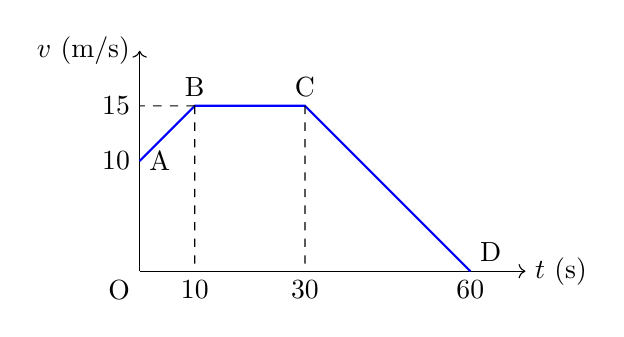
\begin{tikzpicture}[scale=0.7]
				\coordinate (O) at (0,0);
				\coordinate (xaxis) at (7,0);
				\coordinate (yaxis) at (0,4);
				\draw[->] (O)--(xaxis);
				\draw[->] (O)--(yaxis);
				\node[below left] at (O) {O};
				\node[left] at (yaxis) {$v$ (m/s)};
				\node[right] at (xaxis) {$t$ (s)};
				\coordinate (A) at (0,2);
				\coordinate (B) at (1,3);
				\coordinate (C) at (3,3);
				\coordinate (D) at (6,0);				\node[right] at  (A) {A};
				\node[above] at (B) {B};
				\node[above] at (C) {C};
				\node[above right] at (D) {D};
				\draw[thick,blue] (A)--(B)--(C)--(D);
				\path let \p1=(B) in (\x1,0) coordinate (bd) node[below] {10};
				\path let \p2=(C) in (\x2,0) coordinate (cd) node[below] {30};
				\path let \p3=(B) in (0,\y3) coordinate (bl) node[left] {15};
				\node[left] at (A) {10};
				\node[below] at (D) {60};
				\draw[dashed] (B)--(bd);
				\draw[dashed] (C)--(cd);
				\draw[dashed] (B)--(bl);
			\end{tikzpicture}
			%			\includegraphics[scale=0.8]{../figs/VN10-PH-04-L-003-3-V2-04.jpg}
		\end{center}
		\begin{enumerate}[label=\alph*.]
			\item Nêu tính chất chuyển động của mỗi giai đoạn.
			\item Lập phương trình vận tốc của mỗi giai đoạn.
		\end{enumerate}
		
	}
	{\hide{
		\begin{enumerate}[label=\alph*.]
			\item Tính chất chuyển động của mỗi giai đoạn:
			\begin{itemize}
				\item Trên đoạn $AB$: chuyển động nhanh dần đều do đồ thị thể hiện vận tốc tăng với hệ số góc không đổi.
				\item Trên đoạn $BC$: chuyển động thẳng đều do đồ thị thể hiện vận tốc không thay đổi theo thời gian.
				\item Trên đoạn $CD$: chuyển động chậm dần đều đến khi dừng lại do đồ thị thể hiện vận tốc giảm đều về 0.
			\end{itemize}
			\item Phương trình vận tốc của mỗi giai đoạn	
			\begin{align*}
				v_\text{AB}& = \xsi{10 +0,5\cdot t}{\meter/\second} t&(\SI{0}{\second}\leq t \leq \SI{10}{\second}),\\
				v_\text{BC} &= \SI{15}{m/s}.&(\SI{10}{\second}<t\leq \SI{30}{\second}),\\
				v_\text{CD} &= \xsi{15 - 0,5\cdot t}{\meter/\second} & (\SI{30}{\second} < t \leq \SI{60}{\second}).
			\end{align*}
		\end{enumerate}
		
	}}
	
\end{dang}

%				\let\lesson\undefined
\newcommand{\lesson}{\phantomlesson{Bài 7.}}
\setcounter{section}{2}
\section{Bài tập trắc nghiệm}

\begin{enumerate}[label=\bfseries Câu \arabic*:,leftmargin=1.5cm]
	
	\item \mkstar{2}\\
	{Chuyển động thẳng chậm dần đều có
		\begin{mcq}
			\item quỹ đạo là đường cong bất kì.
			\item độ lớn vectơ gia tốc là một hằng số, ngược chiều với vectơ vận tốc của vật.
			\item quãng đường đi được của vật không phụ thuộc vào thời gian.
			\item vectơ vận tốc vuông góc với quỹ đạo của chuyển động.
		\end{mcq}
	
}
\hideall{
\textbf{Đáp án: B.}
}

\item \mkstar{2}\\
{Chọn phát biểu đúng.
	\begin{mcq}
		\item Gia tốc của chuyển động thẳng nhanh dần đều bao giờ cũng lớn hơn gia tốc của chuyển động thẳng chậm dần đều.
		\item Chuyển động thẳng nhanh dần đều có gia tốc lớn thì có vận tốc lớn.
		\item Chuyển động thẳng biến đổi đều có gia tốc tăng, giảm đều theo thời gian.
		\item Gia tốc trong chuyển động thẳng nhanh dần đều có phương, chiều và độ lớn không đổi.
	\end{mcq}

}
\hideall{
\textbf{Đáp án: D.}
}

\item \mkstar{2}\\
{Gọi $v_0$ là vận tốc ban đầu của chuyển động. Công thức liên hệ giữa vận tốc $v$, gia tốc $a$ và quãng đường $s$ vật đi được trong chuyển động thẳng biến đổi đều là
\begin{mcq}(4)
	\item $v+v_0=\sqrt{2as}$.
	\item $v-v_0=\sqrt{2as}$.
	\item $v^2+v^2_0=2as$.
	\item $v^2-v^2_0=2as$.
\end{mcq}
}
\hideall{
\textbf{Đáp án: D.}
}
\item \mkstar{2}\\
{Công thức tính quãng đường đi được của chuyển động thẳng nhanh dần đều là
\begin{mcq}(2)
	\item $s=v_0t+\dfrac{1}{2}at^2$ ($a$ và $v_0$ cùng dấu).
	\item $s=v_0t+\dfrac{1}{2}at^2$ ($a$ và $v_0$ trái dấu).
	\item $x=x_0+v_0t+\dfrac{1}{2}at^2$ ($a$ và $v_0$ cùng dấu).
	\item $x=x_0+v_0t+\dfrac{1}{2}at^2$ ($a$ và $v_0$ trái dấu).
\end{mcq}
}
\hideall{
\textbf{Đáp án: A.}
}

\item \mkstar{2}\\
{Trong công thức tính vận tốc của chuyển động thẳng nhanh dần đều $v = v_0 + at$, thì
\begin{mcq}(2)
	\item $v$ luôn dương.
	\item $a$ luôn dương.
	\item tích $a\cdot v$ luôn dương.
	\item tích $a\cdot v$ luôn âm.
\end{mcq}
}
\hideall{
\textbf{Đáp án: C.}
}

	\item \mkstar{2}\\
	{\begin{minipage}[l]{0.6\textwidth}
			Một vật chuyển động thẳng biến đổi đều mà vận tốc được biểu diễn bởi đồ thị như hình vẽ.\\
			Chuyển động của vật là chuyển động chậm dần đều vì
			\begin{mcq}
				\item đường biểu diễn của vận tốc là đường thẳng.
				\item độ lớn vận tốc tăng theo thời gian.
				\item độ lớn vận tốc giảm đều theo thời gian.
				\item độ lớn vận tốc là hàm bậc nhất theo thời gian.
			\end{mcq}
		\end{minipage}
	\begin{minipage}{0.4\textwidth}
		\begin{center}
			\includegraphics[width=0.5\linewidth]{../figs/VN10-2023-PH-TP009-P-1}
		\end{center}
	\end{minipage}
Gia tốc của chuyển động là
\begin{mcq}(4)
	\item $\SI{-2}{\meter/\second^2}$.
	\item $\SI{2}{\meter/\second^2}$.
	\item $\SI{4}{\meter/\second^2}$.
	\item$\SI{-4}{\meter/\second^2}$.
\end{mcq}
Quãng đường mà vật đi được trong $\SI{2}{\second}$ là 
\begin{mcq}(4)
	\item $\SI{1}{\meter}$.
	\item $\SI{4}{\meter}$.
	\item $\SI{6}{\meter}$.
	\item $\SI{8}{\meter}$.
\end{mcq}
}
\hideall{
\textbf{Đáp án: C - A - B.}\\
Vì độ thị $\left(v-t\right)$ có độ dốc không đổi và $<0$ nên vật chuyển động thẳng chậm dần đều.\\
Gia tốc của chuyển động:
$$a=\dfrac{0-\SI{4}{\meter/\second}}{\SI{2}{\second}}=\SI{-2}{\meter/\second^2}.$$
Quãng đường mà vật đi được trong $\SI{2}{\second}$:
$$s=\dfrac{1}{2}\cdot\left(\SI{4}{\meter/\second}\right)\cdot\left(\SI{2}{\second}\right)=\SI{4}{\meter}.$$
}



\item \mkstar{3}\\
{Một ô tô chuyển động thẳng biến đổi đều từ trạng thái nghỉ, đạt vận tốc $\SI{20}{\meter/\second}$ sau $\SI{5}{\second}$. Quãng đường mà ô tô đã đi được là
\begin{mcq}(4)
	\item $\SI{100}{\meter}$.
	\item $\SI{50}{\meter}$.
	\item $\SI{25}{\meter}$.
	\item $\SI{200}{\meter}$.
\end{mcq}
}
\hideall{
\textbf{Đáp án: B.}\\
Quãng đường ô tô chuyển động:
$$s=\dfrac{1}{2}\cdot\left(\SI{20}{\meter/\second}\right)\cdot\left(\SI{5}{\second}\right)=\SI{50}{\meter}.$$
}

\item \mkstar{3}\\
{Xe ô tô đang chuyển động thẳng với tốc độ $\SI{20}{\meter/\second}$ thì bị hãm phanh chuyển động chậm dần đều. Quãng đường xe đi được từ lúc hãm phanh đến khi xe dừng hẳn là $\SI{100}{\meter}$. Gia tốc của xe là
\begin{mcq}(4)
	\item $\SI{1}{\meter/\second^2}$.
	\item $\SI{-1}{\meter/\second^2}$.
	\item $\SI{-2}{\meter/\second^2}$.
	\item $\SI{5}{\meter/\second^2}$.
\end{mcq}
}
\hideall{
\textbf{Đáp án: C.}\\
Gia tốc của xe:
$$a=\dfrac{v^2-v^2_0}{2s}=\SI{-2}{\meter/\second^2}.$$
}

\item \mkstar{3}\\
{Một ô tô chuyển động chậm dần đều. Sau $\SI{10}{\second}$ vận tốc của ô tô giảm từ $\SI{6}{\meter/\second}$ về $\SI{4}{\meter/\second}$. Quãng đường ô tô đi được trong khoảng thời gian $\SI{10}{\second}$ đó là
	\begin{mcq}(4)
		\item $\SI{70}{\meter}$.
		\item $\SI{50}{\meter}$.
		\item $\SI{40}{\meter}$.
		\item $\SI{100}{\meter}$.
	\end{mcq}

}
\hideall{
\textbf{Đáp án: B.}\\
Quãng đường ô tô đi được trong khoảng thời gian $\SI{10}{\second}$ đó:
$$s=\dfrac{1}{2}\cdot\left(\SI{6}{\meter/\second}+\SI{4}{\meter/\second}\right)\cdot\left(\SI{10}{\second}\right)=\SI{50}{\meter}.$$
}

\item \mkstar{3}\\
{Một ô tô đang chuyển động với vận tốc $\SI{10}{\meter/\second}$ thì bắt đầu tăng ga (tăng tốc), chuyển động nhanh dần đều. Sau $\SI{20}{\second}$ ô tô đạt được vận tốc $\SI{14}{\meter/\second}$. Sau $\SI{50}{\second}$ kể từ lúc tăng tốc, gia tốc và vận tốc của ô tô lần lượt là
\begin{mcq}(2)
	\item $a=\SI{0.2}{\meter/\second^2}$ và $\SI{18}{\meter/\second}$.
	\item $a=\SI{0.2}{\meter/\second^2}$ và $\SI{20}{\meter/\second}$.
	\item $a=\SI{0.4}{\meter/\second^2}$ và $\SI{38}{\meter/\second}$.
	\item $a=\SI{0.1}{\meter/\second^2}$ và $\SI{28}{\meter/\second}$.
\end{mcq}
}
\hideall{
\textbf{Đáp án: B.}\\
Gia tốc của ô tô:
$$a=\dfrac{v-v_0}{t_1}=\SI{0.2}{\meter/\second^2}$$
Vận tốc của ô tô sau $\SI{50}{\second}$:
$$v=v_0+at=\left(\SI{10}{\meter/\second}\right)+\left(\SI{0.2}{\meter/\second^2}\right)\cdot\left(\SI{50}{\second}\right)=\SI{20}{\meter/\second}.$$
}

\item \mkstar{3}\\
{Tàu hỏa đang chuyển động với vận tốc $\SI{60}{\kilo\meter/\hour}$ thì bị hãm phanh chuyển động chậm dần đều. Sau khi đi thêm được $\SI{450}{\meter}$ thì vận tốc của tàu chỉ còn $\SI{15}{\kilo\meter/\hour}$. Quãng đường tàu còn đi thêm được đến khi dừng hẳn là
\begin{mcq}(4)
	\item $\SI{60}{\meter}$.
	\item $\SI{45}{\meter}$.
	\item $\SI{15}{\meter}$.
	\item $\SI{30}{\meter}$.
\end{mcq}
}
\hideall{
\textbf{Đáp án: D.}\\
Ta có:
$$a=\dfrac{v^2-v^2_0}{2s}=\dfrac{0-v^2_0}{2s'}\Rightarrow s'=\SI{480}{\meter}$$
Quãng đường tàu hoả đi thêm cho đến khi dừng lại:
$$\Delta s=s'-s=\SI{30}{\meter}.$$
}
	\item \mkstar{3}\\
	{\begin{minipage}[l]{0.65\textwidth}
			Đồ thị vận tốc - thời gian của một tàu hỏa đang chuyển động thẳng có dạng như hình bên. Thời điểm $t = 0$ là lúc tàu đi qua sân ga. Vận tốc của tàu sau khi rời sân ga được $\SI{80}{\meter}$ là
			\begin{mcq}(2)
				\item $\SI{4}{\meter/\second}$.
				\item $\SI{6}{\meter/\second}$.
				\item $\SI{8}{\meter/\second}$.
				\item $\SI{10}{\meter/\second}$.
			\end{mcq}
		\end{minipage}
		\begin{minipage}{0.35\textwidth}
			\begin{center}
				\includegraphics[width=0.5\linewidth]{../figs/VN10-2022-PH-TP008-P-3}
			\end{center}
		\end{minipage}
	}
	\hideall{
		\textbf{Đáp án: B.}\\
		Gia tốc của tàu:
		$$a=\dfrac{\SI{12}{\meter/\second}-\SI{2}{\meter/\second}}{\SI{50}{\second}}=\SI{0.2}{\meter/\second^2}$$
		Vận tốc của tàu sau khi rời ga được $\SI{80}{\meter}$:
		$$v=\sqrt{v^2_0+2as}=\SI{6}{\meter/\second}.$$
		
	}

\item \mkstar{3}\\
{\begin{minipage}[l]{0.65\textwidth}
Một vật chuyển động thẳng biến đổi đều có đồ thị vận tốc $v$ theo thời gian $t$ như hình vẽ. Phương trình vận tốc của vật là
		\begin{mcq}(2)
			\item $v=15-t \left(\si{\meter/\second}\right)$.
			\item $v=15+t \left(\si{\meter/\second}\right)$.
			\item $v=10-5t \left(\si{\meter/\second}\right)$.
			\item $v=10-5t \left(\si{\meter/\second}\right)$.
		\end{mcq}
	\end{minipage}
	\begin{minipage}{0.35\textwidth}
		\begin{center}
			\includegraphics[width=0.6\linewidth]{../figs/VN10-2023-PH-TP009-P-2}
		\end{center}
	\end{minipage}
}
\hideall{
\textbf{Đáp án: A.}\\
Gia tốc của tàu:
$$a=\dfrac{0-\SI{10}{\meter/\second}}{\SI{10}{\second}}=\SI{-1}{\meter/\second^2}$$
Phương trình vận tốc của tàu:
$$v=v_0+at=v_0-t$$
Khi $t=\SI{5}{\second}$ thì $v=\SI{10}{\meter/\second} \Rightarrow v_0=\SI{15}{\meter/\second}$.\\
Như vậy: $v=15-t\qquad \left(\si{\meter/\second}\right)$.
}

\item \mkstar{3}\\
{\begin{minipage}[l]{0.6\textwidth}
		Một vật chuyển động có đồ thị vận tốc - thời gian như hình vẽ. Quãng đường đi được trong giai đoạn chuyển động thẳng chậm dần đều là
		\begin{mcq}(2)
			\item $\SI{62.5}{\meter}$.
			\item $\SI{75}{\meter}$.
			\item $\SI{37.5}{\meter}$.
			\item $\SI{100}{\meter}$.
		\end{mcq}
	\end{minipage}
\begin{minipage}{0.4\textwidth}
	\begin{center}
		\includegraphics[width=0.6\linewidth]{../figs/VN10-2023-PH-TP009-P-3}
	\end{center}
\end{minipage}
}
\hideall{
\textbf{Đáp án: C.}\\
Quãng đường vật đi được trong giai đoạn chuyển động thẳng chậm dần đều:
$$s=\dfrac{1}{2}\cdot\left(\SI{5}{\meter/\second}\right)\cdot\left(\SI{15}{\second}\right)=\SI{37.5}{\meter}.$$
}




\item \mkstar{4}\\
{Một xe chuyển động nhanh dần đều với vận tốc đầu $\SI{18}{\kilo\meter/\hour}$. Trong giây thứ 5 xe đi được $\SI{14}{\meter}$. \\
	Gia tốc của xe là
	\begin{mcq}(4)
		\item $\SI{4}{\meter/\second^2}$.
		\item $\SI{3}{\meter/\second^2}$.
		\item $\SI{2}{\meter/\second^2}$.
		\item $\SI{6}{\meter/\second^2}$.
	\end{mcq}
Quãng đường đi được trong giây thứ 10
\begin{mcq}(4)
	\item $\SI{24}{\meter}$.
	\item $\SI{34}{\meter}$.
	\item $\SI{14}{\meter}$.
	\item $\SI{44}{\meter}$.
\end{mcq}
}
\hideall{
\textbf{Đáp án: C - A.}\\
$$s=v_0\cdot t+\dfrac{1}{2}\cdot at^2$$
Quãng đường xe đi được trong giây thứ 5:
$$\Delta s=s_{\left(t=5\right)}-s_{\left(t=4\right)}=\SI{14}{\meter}\Rightarrow a=\SI{2}{\meter/\second^2}$$
Quãng đường xe đi được trong giây thứ 10:
$$\Delta s'=s_{\left(t=5\right)}-s_{\left(t=9\right)}=\SI{24}{\meter}.$$
}
\end{enumerate}
\section{Bài tập tự luận}
\begin{enumerate}[label=\bfseries Bài \arabic*:,leftmargin=1.5cm]
	\item \mkstar{3}
	
	{ Từ các đồ thị trong hình:
		\begin{center}
			\includegraphics[scale=1]{../figs/VN10-2022-PH-TP012-1.jpg}
		\end{center}
		
		\begin{enumerate}[label=\alph*)]
			\item Hãy viết công thức về mối liên hệ giữa $v$ với $a$ và $t$ của từng chuyển động ứng với từng đồ thị trong hình.
			\item Chuyển động nào là chuyển động nhanh dần dều, chậm dần đều?
		\end{enumerate}
		
	}
	
	\hideall{
		
		\begin{enumerate}[label=\alph*)]
			\item 
			- Đồ thị a: $$v=at.$$
			
			- Đồ thị b: $$v = v_0 + at.$$
			
			- Đồ thị c: $$v = v_0 -at.$$
			\item 
			
			- Chuyển động nhanh dần đều là: đồ thị a và b.
			
			- Chuyển động chậm dần đều: đồ thị c.
			
			
			
			
		\end{enumerate}
		
	}

	
	\item \mkstar{2}
	
	{
		Trong một cuộc thi chạy, một vận động viên chạy nhanh dần đều từ trạng thái đứng yên với gia tốc $\SI{5}{m/s}^2$ trong 2 giây đầu tiên. Tính tốc độ của vận động viên sau 2 giây.
	}
	\hideall{
		
		Tốc độ của vận động viên sau 2 giây đầu tiên:
		
		$$a = \dfrac{v_2 - v_1}{t} \Rightarrow v_2 = at = \SI{10}{m/s}.$$
	}
	
	\item \mkstar{3}
	
	{
		Một xe máy đang chuyển động thẳng với vận tốc $\SI{10}{m/s}$ thì tăng tốc. Sau $\SI{5}{s}$ đạt vận tốc $\SI{12}{m/s}.$
		
		\begin{enumerate}[label=\alph*)]
			\item Tính gia tốc của xe.
			\item Nếu sau khi đạt vận tốc $\SI{12}{m/s}$, xe chuyển động chậm dần với gia tốc có độ lớn bằng gia tốc trên thì sau bao lâu xe dừng lại?
		\end{enumerate}
	}
	\hideall{
		
		\begin{enumerate}[label=\alph*)]
			\item Gia tốc của xe
			
			$$a = \dfrac{\Delta v}{\Delta t} = \SI{0,4}{m/s}^2.$$
			
			\item Thời gian xe dừng lại
			
			$$\Delta t' = \dfrac{\Delta v'}{a} = \SI{30}{s}.$$
		\end{enumerate}
		
	}

	
	
	
	\item \mkstar{3}\\
{Một ô tô đang chuyển động thẳng đều với vận tốc $\SI{45}{\kilo\meter/\hour}$ bỗng tăng ga chuyển động nhanh dần đều.
	\begin{enumerate}[label=\alph*.]
		\item Tính gia tốc của xe biết rằng sau $\SI{30}{\second}$ ô tô đạt vận tốc $\SI{72}{\kilo\meter/\hour}$.
		\item Trong quá trình tăng tốc nói trên, vào thời điểm nào kể từ lúc tăng tốc, vận tốc của xe là $\SI{64.8}{\kilo\meter/\hour}$?
	\end{enumerate}
}
\hideall{Đổi đơn vị $\SI{45}{km/h} = \SI{12,5}{m/s};\ \SI{72}{km/h} = \SI{20}{m/s}$.
	
	Chọn chiều dương là chiều chuyển động.
	
	a. Gia tốc của xe là
	$$a = \dfrac{v-v_0}{t} =\dfrac{\SI{20}{\meter/\second}-\SI{12.5}{\meter/\second}}{\SI{30}{\second}}= \SI{0,25}{m/s}^2.$$
	
	b. Đổi đơn vị $\SI{64,8}{km/h} = \SI{18}{m/s}$.
	
	Xe đạt vận tốc $\SI{64,8}{km/h}$ vào thời điểm 
	$$t= \dfrac{v'-v_0}{a}=\dfrac{\SI{18}{\meter/\second}-\SI{12.5}{\meter/\second}}{\SI{0.25}{\meter/\second^{2}}} = \SI{22}{s}.$$
	
}



	\item \mkstar{3}\\
	{Một người đi xe đạp lên dốc dài $\SI{50}{\meter}$. Tốc độ ở dưới chân dốc là $\SI{18}{\kilo\meter/\hour}$ và ở đầu dốc lúc đến nơi là $\SI{3}{\meter/\second}$. Tính gia tốc của chuyển động và thời gian lên dốc. Coi chuyển động trên là chuyển động chậm dần đều.
	
}
	\hideall{
		Gia tốc của người đi xe đạp:
		$$a=\dfrac{v^2-v^2_0}{2s}=\SI{-0.16}{\meter/\second^2}$$
		Thời gian lên dốc:
		$$\Delta t=\dfrac{\Delta v}{a}=\SI{12.5}{\second}.$$
}

\item \mkstar{3}\\
Một người đạp xe trên đường thẳng với tốc độ $\SI{4}{\meter/\second}$ thì bóp thắng để giảm tốc với gia tốc có độ lớn không đổi là $\SI{0.5}{\meter/\second^2}$. Xác định thời gian và quãng đường xe đi được từ khi bóp thắng đến khi dừng lại.
\hideall{
Quãng đường xe đi được từ khi bóp thắng đến khi dừng lại:
$$s=\dfrac{0-v^2_0}{2a}=\dfrac{-\left(\SI{4}{\meter/\second^2}\right)^2}{2\cdot\left(-\SI{0.5}{\meter/\second^}\right)}=\SI{16}{\meter}.$$
Thời gian từ khi bóp thắng đến khi dừng lại:
$$\Delta t=\dfrac{\Delta v}{a}=\dfrac{0-\SI{4}{\meter/\second}}{-\SI{0.5}{\meter/\second^2}}=\SI{8}{\second}.$$
}

\item \mkstar{3}\\
Khi đang chạy với tốc độ $\SI{36}{\kilo\meter/\hour}$ thì ô tô bắt đầu chạy xuống dốc. Nhưng do bị mất phanh nên ô tô chuyển động thẳng nhanh dần đều với gia tốc $\SI{0.2}{\meter/\second}$ xuống hết dốc có độ dài $\SI{960}{\meter}$. Khoảng thời gian ô tô chạy xuống hết đoạn dốc là bao nhiêu?
\hideall{
Thời gian ô tô chạy xuống hết đoạn dốc:
\begin{eqnarray*}
	s&=&v_0t+\dfrac{1}{2}at^2\\
	\Leftrightarrow 960&=&10t+\dfrac{1}{2}\cdot0,2t^2\\
	\Rightarrow t&=&\SI{60}{\second}
\end{eqnarray*}
}

	\item \mkstar{3}
	
	
	{Đồ thị vận tốc - thời gian ở hình mô tả chuyển động của một chú chó con đang chạy trong một ngõ thẳng và hẹp.
		\begin{center}
			\includegraphics[scale=1]{../figs/VN10-2022-PH-TP012-5.jpg}
		\end{center}
		
		\begin{enumerate}[label=\alph*)]
			\item Hãy mô tả chuyển động của chú chó.
			\item Tính quãng đường đi được và độ dịch chuyển của chú chó sau $\SI{2}{s}$; $\SI{4}{s}$; $\SI{7}{s}$ và $\SI{10}{s}$ bằng đồ thị.
		\end{enumerate}
	}
	
	\hideall
	{	
		\begin{enumerate}[label=\alph*)]
			\item 
			- Trong 2 giây đầu tiên: chuyển động thẳng đều với vận tốc $\SI{1}{m/s}$.
			
			- Từ giây thứ 2 đến giây thứ 4: chuyển động nhanh dần đều.
			
			- Từ giây 4 đến giây 7: chuyển động chậm dần.
			
			- Từ giây 4 đến giây 8: dừng lại.
			
			- Từ giây 8 đến giây 9: chuyển động nhanh dần theo chiều âm.
			
			- Từ giây 9 đến giây 10 chuyển động thẳng đều với vận tốc $-\SI{1}{m/s}$.
			
			
			\item 
			- Sau 2 giây:
			
			$$s_1 = d_1 = v_1 t_1 = \SI{2}{m/s}.$$
			
			- Sau 4 giây:
			
			$$s_2 = d_2 = s_1 + \dfrac{1}{2} (1+3)2 = \SI{6}{m}.$$
			
			- Sau 7 giây:
			
			$$s_3 =d_3= s_2 + \dfrac{1}{2} (7-4)3 = \SI{10,5}{m}.$$
		
			- Sau 10 giây:
			
			+ Quãng đường:
			
			Từ giây 7 – 8: đứng yên
			
			$$s_4 = s_3 + s' = \text{10,5} + \text{0,5} + 1 = \SI{12}{m}.$$
			
			+ Độ dịch chuyển:
			
			$$d_4 = d_3 + d' = \text{10,5} - \text{0,5} - 1 = \SI{9}{m}.$$
			
		\end{enumerate}
	}

\item \mkstar{3}\\
{Dựa vào đồ thị vận tốc - thời gian ở hình \ref{fig:TP009-P-1}, hãy xác định tính chất chuyển động và độ dịch chuyển trong từng giai đoạn chuyển động của xe.
	\begin{center}
		\includegraphics[width=0.35\linewidth]{../figs/VN10-2023-PH-TP009-P-4}
		\captionof{figure}{}
		\label{fig:TP009-P-4}
	\end{center}

}
\hideall{
\begin{itemize}
	\item Trong giai đoạn từ $\SI{0}{\second}$ đến $\SI{40}{\second}$, vật chuyển động nhanh dần đều.\\
	Độ dịch chuyển của vật trong gia đoạn này:
	$$d_1=\dfrac{1}{2}\cdot\left(\text{OA}+\text{BC}\right)\cdot\text{OC}=\SI{3200}{\meter}.$$
	\item Trong giai đoạn từ $\SI{40}{\second}$ đến $\SI{80}{\second}$, vật chuyển động thẳng đều với tốc độ $\SI{120}{\meter/\second}$.\\
	Độ dịch chuyển của vật trong giai đoạn này:
	$$d_2=\text{BC}\cdot\text{CE}=\SI{4800}{\meter}.$$
	\item Trong giai đoạn từ $\SI{80}{\second}$ đến $\SI{160}{\second}$, vật chuyển động chậm dần đều với gia tốc $a_3=\dfrac{v_\text{F}-v_\text{D}}{t_\text{F}-t_\text{E}}=\SI{-1.5}{\meter/\second^2}.$\\
	Độ dịch chuyển của vật trong giai đoạn này:
	$$d_3=\dfrac{1}{2}\cdot\text{DE}\cdot\text{EF}=\SI{4800}{\meter}.$$
	
\end{itemize}

}

	\item \mkstar{4}
	
	
	{Một vận động viên đua xe đạp đường dài vượt qua vạch đích với vận tốc $\SI{10}{m/s}$. Sau đó vận động viên này đi chậm dần đều thêm $\SI{20}{m}$ mới dừng lại. Coi chuyển động của vận động viên là thẳng.
		\begin{enumerate}[label=\alph*)]
			\item Tính gia tốc của vận động viên trong đoạn đường sau khi qua vạch đích.
			\item Tính thời gian vận động viên đó cần để dừng lại kể từ khi cán đích.
			\item Tính tốc độ trung bình của người đó trên quãng đường dừng xe.
		\end{enumerate}
	}
	
	\hideall
	{	
		\begin{enumerate}[label=\alph*)]
			\item Gia tốc của vận động viên trong đoạn đường sau khi qua vạch đích
			
			$$v^2 - v_0^2 = 2ad \Rightarrow a = -\SI{2,5}{m/s}^2.$$
			
			\item Thời gian vận động viên đó cần để dừng lại kể từ khi cán đích
			
			$$a = \dfrac{\Delta v}{\Delta t} \Rightarrow  \Delta t = \SI{4}{s}.$$
			
			\item Tốc độ trung bình của người đó trên quãng đường dừng xe
			
			$$v = \dfrac{d}{t} = \SI{5}{m/s}.$$
		\end{enumerate}
	}
\end{enumerate}

%				\let\lesson\undefined
\newcommand{\lesson}{\phantomlesson{Bài 7: Gia tốc. Chuyển động thẳng biến đổi đều}}
\chapter[Phương trình toạ độ của vật chuyển động thẳng biến đổi đều (đọc thêm)]{Phương trình toạ độ của vật chuyển động thẳng biến đổi đều (đọc thêm)}
\setcounter{section}{0}
\section{Lý thuyết}
\subsection{Phương trình toạ độ của chất điểm chuyển động thẳng biến đổi đều}
Phương trình chuyển động của vật là phương trình mô tả sự thay đổi tọa độ của vật theo thời gian. \\
Để lập phương trình toạ độ của vật chuyển động thẳng biến đổi đều, ta thực hiện các bước như sau:
\begin{itemize}
	\item Chọn hệ quy chiếu gồm:
	\begin{itemize}
		\item Gốc tọa độ (thường là vị trí xuất phát của một vật);
		\item Mốc thời gian (thường là thời điểm bắt đầu chuyển động của một vật);
		\item Chiều dương (thường là chiều chuyển động của một vật).
	\end{itemize}
	\item Xét một điểm chuyển động thẳng biến đổi đều trên đường thẳng O$x$. Ở thời điểm ban đầu ($t_0$), chất điểm ở vị trí A có tọa độ $x_{0}$  với vận tốc ban đầu $v_0$ và gia tốc $a$. Mốc thời gian được chọn lúc bắt đầu chuyển động. Ở thời điểm $t$, chất điểm ở vị trí B có tọa độ $x$ như hình vẽ.  	
	\begin{center}
		\begin{tikzpicture}
			\coordinate (laxis) at (-0.5,0);
			\coordinate (O) at (0,0);
			\coordinate (A) at (2,0);
			\coordinate (va) at ($(A)+(1,0)$);
			\coordinate (raxis) at (8,0);
			\coordinate (ldaxis) at (-0.5,-1);
			\coordinate (Od) at (0,-1);
			\coordinate (Ad) at (2,0);
			\coordinate (B) at (5,-1);
			\coordinate (vb) at ($(B)+(2,0)$);
			\coordinate (rdaxis) at (8,-1);
			\draw[->] (laxis) -- (raxis);
			\draw[->] (ldaxis) -- (rdaxis);
			
			
			\draw[->,ultra thick,blue] (A) -- (va);
			\draw[->,ultra thick,green!60!black] (B) -- (vb);
			\node[above=2mm] at (A) {A};
			\node[below left=1mm and 0.5mm] at (A) {$x_0$};
			\node[above=2mm] at (B) {B};
			\node[below left=1mm and 0.5mm] at (B) {$x$};
			\node[above=2mm] at (O) {O};
			
			%		\node[above=2mm] at (Od) {O};
			%		\node[below=2mm] at (C) {C};
			\node[right] at (raxis) {$x$};
			\node[above=1mm] at (va) {$\vec{v}_{0}$};
			\node[above=1mm] at (vb) {$\vec{v}$};
			
			\node[left=3cm,anchor=west] at (laxis) {thời điểm $t_0$};
			\node[left=3cm,anchor=west] at (ldaxis) {thời điểm $t> t_0$};
			\foreach \i in {O,Od,B,A}
			{
				\filldraw (\i) circle (2pt);
			}
			
			%		\coordinate (odd) at ($(O)-(0,2)$);
			\coordinate (add) at ($(A)-(0,2)$);
			\coordinate (bdd) at ($(B)-(0,1)$);
			%		\draw[<->,thick] (odd) -- (add);
			\draw[<->] (add) -- (bdd) node[midway,fill=pagecol] {$d$};
			\draw[dashed] (O)--(Od);
			\draw[dashed] (A)--(add);
			\draw[dashed] (B)--(bdd);
			
		\end{tikzpicture}
	\end{center}
	Phương trình chuyển động của vật có dạng tổng quát như sau:
	\begin{equation*}
		x=x_0+d=x_0+v_0\cdot(t-t_0)+\dfrac{1}{2}a\cdot(t-t_0)^2\qquad\textrm{ với }(t\geq t_0),
	\end{equation*}
	Thông thường, để thuận tiện trong tính toán, ta chọn thời điểm $t_0=0$, khi đó phương trình chuyển động của chất điểm trở thành 
	\begin{equation*}
		x=x_0+v_0t+\dfrac{1}{2}at^{2}.
	\end{equation*}
\end{itemize}	
\subsection{Điều kiện để hai vật gặp nhau}
Hai vật gặp nhau khi chúng có cùng tọa độ:
\begin{equation*}
	x_1=x_2.
\end{equation*}
\subsection{Khoảng cách giữa hai vật trong quá trình chuyển động}
Khoảng cách giữa hai vật tại thời điểm $t$ bất kì là:
\begin{equation*}
	\Delta x=\left|x_1-x_2\right|.
\end{equation*}
\section{Mục tiêu bài học - Ví dụ minh họa}
\begin{dang}{Xác định quãng đường, vận tốc, gia tốc, thời gian \\thông qua phương trình chuyển động }
	\viduii{2}{Một vật chuyển động có phương trình toạ độ theo thời gian: $x = 6t^2 - 18t + 12 \ (\text{cm, s})$. Hãy xác định:
		\begin{enumerate}[label=\alph*.]
			\item Vận tốc đầu, gia tốc của chuyển động và cho biết tính chất của chuyển động.
			\item Vận tốc của vật ở thời điểm $t = \SI{2}{\second}$.
		\end{enumerate}
	}
	{\hide{
		\begin{enumerate}[label=\alph*.]
			\item Đối chiếu phương trình 
			$$x = 6t^2 - 18t + 12 \ \text{cm}$$
			với phương trình chuyển động
			$$x=x_0+v_0t+\dfrac{1}{2}at^{2}$$
			ta suy ra
			$$v_0 = \SI{-18}{\centi\meter/\second};\qquad a =\SI{12}{\centi\meter/\second^{2}}.$$
			
			Vật chuyển động chậm dần đều do gia tốc và vận tốc trái dấu với nhau.
			\item Thay các giá trị vận tốc và gia tốc đã tìm được vào phương trình vận tốc, ta suy ra vận tốc của vật ở thời điểm $t=\SI{2}{\second}$
			$$v =v_0 +at =\SI{-18}{\centi\meter/\second}+\SI{12}{\centi\meter/\second^{2}}\cdot\SI{2}{\second}=\SI{6}{\centi\meter/\second}.$$
		\end{enumerate}
	}}
	
	\viduii{3}{Một vật chuyển động thẳng có phương trình toạ độ theo thời gian: $x = 4t^2 + 20t\ (\text{m})$. Xác định độ dịch chuyển của vật từ thời điểm $t_1 = \SI{2}{s}$ đến thời điểm $t_2 = \SI{5}{s}$.
	}
	{\hide{
		Vị trí của vật ở thời điểm  $\SI{2}{\second}$  
		
		$$x_1 = 4t_1^2 + 20t_1 =\SI{56}{\meter}.$$
		
		Vị trí của vật ở thời điểm  $\SI{5}{\second}$ 
		
		$$x_2 = 4t_2^2 + 20t_2 =\SI{200}{\meter}.$$
		
		Độ dịch chuyển của vật trong thời gian từ $\SI{2}{\second}$  đến $\SI{5}{\second}$ là:
		$$d = x_2 - x_1 = \SI{144}{\meter}.$$
		
	}}

	\viduii{3}{Vật chuyển động thẳng có phương trình: $x = 2t^2 - 4t + 10$ (đơn vị của $x$ và $t$ lần lượt là mét và giây). Vật sẽ dừng lại tại vị trí
		\begin{mcq}(4)
			\item $\SI{6}{m}.$
			\item $\SI{4}{m}.$
			\item $\SI{10}{m}.$
			\item $\SI{8}{m}.$
		\end{mcq}
	}
	{\hide{
		Vật sẽ dừng lại khi vận tốc $v = 0$.
		
		Từ phương trình chuyển động ta suy ra các giá trị vận tốc ban đầu và gia tốc 
		$$v_0=\SI{-4}{\meter/\second},	\qquad a=\SI{4}{\meter/\second^{2}}.$$
		
		Sử dụng phương trình vận tốc, ta suy ra thời điểm vật dừng lại
		\begin{align*}
			v=v_0+at=0 \quad\Rightarrow\quad t=-\dfrac{v_0}{a}=-\dfrac{\SI{-4}{\meter/	\second}}{\SI{4}{\meter/\second^{2}}}=\SI{1}{\second}.
		\end{align*}		
		Thay $t =\SI{1}{\second}$ vào phương trình chuyển động ta được vị trí dừng lại của vật 
		$$x = 2t^2 - 4t + 10=\SI{8}{\meter}.$$
		
		\textbf{Đáp án: D}.
	}}
\end{dang}
\begin{dang}{Xây dựng phương trình\\ chuyển động thẳng biến đổi đều}
	\viduii{2}{Một vật chuyển động thẳng chậm dần đều với tốc độ ban đầu $\SI{3}{\meter/\second}$ và gia tốc có độ lớn $\SI{2}{\meter/\second^2}$. Biết thời điểm ban đầu vật ở gốc tọa độ và chuyển động ngược chiều dương của trục tọa độ. Viết phương trình chuyển động của vật.
	}
	{\hide{
		Chọn gốc thời gian là khi vật bắt đầu chuyển động.
		
		Vì vật chuyển động chậm dần đều ngược chiều dương nên
		\begin{equation*}
			\left\{
			\begin{array}{rcl}
				a\cdot v &<&0\\
				v &<& 0
			\end{array}
			\right.
			\quad
			\Rightarrow 
			\left\{
			\begin{array}{rcl}
				a &>& 0\\
				v &<& 0.
			\end{array}
			\right.
		\end{equation*}
		
		Kết hợp với các dữ kiện của đề bài, ta suy ra
			\begin{align*}
				\begin{cases}
					a=\SI{2}{\meter/\second^2}\\
					v=\SI{-3}{\meter/\second}\\
					x_0=\SI{0}{\meter} \qquad\text{(vì ban đầu vật ở gốc toạ độ.)}
				\end{cases}
			\end{align*}
		Do đó, phương trình chuyển động của vật có dạng
		$x=-3t+t^2$ (m, s).
	}}

	\viduii{3}{Một đoạn dốc thẳng dài $\SI{62,5}{m}$, Nam đi xe đạp và khởi hành từ chân dốc đi lên với $v_0 =\SI{18}{km/h}$ chuyển động chậm dần đều với gia tốc có độ lớn $\SI{0,2}{m/s}^2$.
		\begin{enumerate}[label=\alph*.]
			\item Viết phương trình chuyển động của Nam.
			\item Nam đi hết đoạn dốc trong bao lâu?
		\end{enumerate}
	}
	{\hide{
		Đổi đơn vị $$\SI{18}{km/h} = \dfrac{\SI{18e3}{\meter}}{\SI{3600}{\second}}=\SI{5}{m/s}.$$
		
		Chọn gốc toạ độ tại chân dốc, chiều dương từ chân dốc đến đỉnh dốc, gốc thời gian là khi Nam bắt đầu lên dốc.
		\begin{enumerate}[label=\alph*.]
			\item Khi nam lên dốc, Nam đi theo chiều dương nên $v>0$.
			
			Chuyển động chậm dần đều: 
			$$a\cdot v<0 \Rightarrow a<0.$$
			
			Phương trình chuyển động:
			$$x =x_0 +v_0t+\dfrac{1}{2}at^2 = 5t - \text{0,1}t^2.$$
			\item Thời gian đi hết đoạn dốc
			$$\text{62,5} =5t - \text{0,1}t^2 \Rightarrow t = \SI{25}{s}.$$
		\end{enumerate}
	}}
\end{dang}

\begin{dang}{Xác định vị trí, thời điểm hai vật gặp nhau}
	\viduii{3}{Một xe ô tô bắt đầu chuyển động thẳng nhanh dần đều với gia tốc $\SI{0,5}{\meter/\second^{2}}$ đúng lúc một xe máy chuyển động thẳng đều với tốc độ $\SI{36}{\kilo\meter/\hour}$ vượt qua nó.
		Xác định thời điểm và vị trí hai xe gặp nhau lần nữa và vận tốc xe ô tô khi đó?
		Xác định thời điểm để hai xe cách nhau một quãng đường là $\SI{100}{\meter}$.
		
	}
	{\hide{
		Chọn chiều dương là chiều chuyển động của ô tô, gốc tọa độ tại vị trí xuất phát, gốc thời gian là lúc xe ô tô khởi hành.
		
		Xe ô tô có các điều kiện đầu: 
		$$x_{10} = \SI{0}{\meter};\qquad  v_{10} = \SI{0}{\meter/\second};\qquad a_1 = \SI{0.5}{\meter
			/\second^{2}}$$	
		nên có phương trình chuyển động 
		$$x_1 = x_{10}+v_{10}t+\dfrac{1}{2}a_{1}t^{2}=0,25t^2\quad \left(\si{\meter}, \si{\second}\right).$$
		
		Xe máy có các điều kiện đầu
		$$x_{20} = 0;\qquad v_{20} =\SI{36}{\kilo\meter/\hour}=\SI{10}{\meter/\second};\qquad a_{2} = \SI{0}{\meter/\second^{2}}$$	
		nên có phương trình chuyển động 
		$$x_2 =x_{20}+v_{20}t+\dfrac{1}{2}a_2t^2=10t\quad \left(\si{\meter}, \si{\second}\right).$$
		
		Khi hai xe gặp nhau thì toạ độ của chúng bằng nhau
			$$x_1=x_2$$
			$$\Rightarrow0,25t^2=10t$$
		\begin{align*}
		\Rightarrow t=\SI{0}{\second}\quad \text{hoặc} \quad	t=\SI{40}{\second}
		\end{align*}
		trong đó nghiệm $t=0$ ứng với thời điểm hai xe gặp nhau lúc đầu, còn nghiệm $t=\SI{40}{\second}$ là nghiệm ta cần tìm. 
		
		Vị trí 2 xe gặp nhau 
		$$x_1=x_2=v_{20}t =\left(\SI{10}{\meter/\second}\right)\cdot\left(\SI{40}{\second}\right)= \SI{400}{m}.$$
		
		Vận tốc ô tô khi đó 
		$$v_1 = v_{10}+ a_1t = \SI{0}{\meter/\second}+\left(\SI{0.5}{\meter/\second^{2}}\right)\cdot\left(\SI{40}{\second}\right)=\SI{20}{m/s}.$$  
	}}

	\viduii{3}{
		Trong một chuyến từ thiện của trung tâm A thì mọi người dừng lại bên đường uống nước. Sau đó, ngay thời điểm ô tô bắt đầu chuyển động nhanh dần đều với gia tốc $\SI{0,5}{m/s}^2$ thì có một xe khách vượt qua xe với tốc độ $\SI{18}{km/h}$ và gia tốc $\SI{0,3}{m/s}^2$. Hỏi ô tô đuổi kịp xe khách sau khi đi quãng đường bao xa, và tính vận tốc của ô tô lúc đó.
	}
	{\hide{
		Chọn chiều dương là chiều chuyển động của ô tô, gốc tọa độ tại vị trí uống nước, gốc thời gian là lúc xe ô tô khởi hành.
		
		Từ các điều kiện ban đầu của ô tô
		$$x_{10} = 0,\quad v_{10} = 0,\quad a_{1} = \SI{0,5}{m/s}^2,$$	
		ta suy ra phương trình chuyển động của ô tô
		$$x_1 = \text{0,25}t^2.$$
		
		Từ các điều kiện ban đầu của xe khách, ta suy ra được phương trình chuyển động của xe khách
		\begin{equation*}
			\begin{gathered}
				x_{20} = 0,\quad v_{20} =\SI{18}{km/h}=\SI{5}{m/s},\quad a_{2} = \SI{0,3}{m/s}^2\\
				\Rightarrow\quad x_2 =5t+\text{0,15}t^2.
			\end{gathered}
		\end{equation*}
		
		Thời điểm hai xe gặp nhau được xác định từ phương trình 
		$$x_1=x_2 \quad\Rightarrow\quad \text{0,25}t^2=5t+\text{0,15}t^2 \quad\Rightarrow\quad t=\SI{0}{\second}\quad\vee\quad t =\SI{50}{s}.$$
		Ta chọn nghiệm $t =\SI{50}{s}$ là thời điểm gặp nhau sau khi ô tô đã xuất phát. 
		
		Vận tốc của ô tô khi đó
		$$v_1 = v_{10}+ a_1t = \SI{0}{\meter/\second}+\SI{0.5}{\meter/\second^{2}}\cdot\SI{50}{\second}=\SI{25}{m/s}.$$  
		
		Quãng đường ô tô đã đi được cho đến khi gặp nhau 
		$$s=x-x_0 =\text{0,25}t^2 = \SI{625}{\meter}.$$	
	}}
\end{dang}
\begin{dang}{Xác định vận tốc, khoảng cách giữa hai vật\\ chuyển động thẳng biến đổi đều}
	\viduii{3}{Một xe ô tô bắt đầu chuyển động thẳng nhanh dần đều với gia tốc $\SI{0,5}{m/s}^2$ đúng lúc một xe máy chuyển động thẳng đều với vận tốc $\SI{36}{km/h}$ vượt qua nó. Xác định thời điểm để hai xe cách nhau một quãng đường là $\SI{100}{m}$.
	}
	{\hide{
		Chọn chiều dương là chiều chuyển động của ô tô, gốc tọa độ tại vị trí xuất phát, gốc thời gian là lúc xe ô tô khởi hành.
		
		Xe ô tô có các điều kiện ban đầu
		$$x_{10} = \SI{0}{\meter};\qquad  v_{10} = \SI{0}{\meter/\second};\qquad a_1 = \SI{0.5}{\meter
			/\second^{2}}$$	
		nên có phương trình chuyển động 
		$$x_1 = x_{10}+v_{10}t+\dfrac{1}{2}a_{1}t^{2}=\dfrac{1}{2}a_1t^2=\SI{0.25}{}t^{2}.$$
		
		Xe máy có các điều kiện ban đầu
		$$x_{20} = 0;\qquad v_{20} =\SI{36}{\kilo\meter/\hour}=\SI{10}{\meter/\second};\qquad a_{2} = \SI{0}{\meter/\second^{2}}$$	
		nên có phương trình chuyển động 
		$$x_2 =x_{20}+v_{20}t+\dfrac{1}{2}a_2t^2=v_{20}t=\SI{10}{}t.$$
		
		Để 2 xe cách nhau $\SI{40}{m}$ thì 
		$$|x_1-x_2| = 100.$$
		$$\Rightarrow \left[\begin{array}{ll}{x_1-x_2 =100}&\\{x_2-x_1 =100.}&\end{array}\right.$$
		
		$$\Rightarrow 
		\left[\begin{array}{ll}{\text{0,25}t^2 -10t=100 \Rightarrow t\approx\SI{48,28}{s}}&\\{10t-\text{0,25}t^2=100\Rightarrow t =\SI{20}{s}.}&\end{array}\right.$$
		
		\luuy{Đôi khi các phương trình cho ta nhiều nghiệm $t$, ta cần phân tích ý nghĩa của nghiệm và lựa chọn nghiệm phù hợp với thời điểm ta quan tâm. 
			
			Chẳng hạn trong  bài toán này, các phương trình cho ba nghiệm: $t_1\approx\SI{-8.28}{\second}, t_2=\SI{20}{\second},t_3\approx\SI{48.28}{\second}$. Nghiệm $t_1$ tương ứng với thời điểm trước khi xe hai xe gặp nhau lần đầu, lúc đó xe máy đang ở phía sau của ô tô và chuẩn bị vượt qua ô tô. Nghiệm $t_2$ ứng với thời điểm ô tô đang đuổi theo xe máy, và còn cách xe máy \SI{100}{\meter}. Nghiệm $t_3$ ứng với thời điểm ô tô đã vượt qua xe máy và đã bỏ xa xe máy \SI{100}{\meter}. Do đề bài chỉ cho ta biết về chuyển động hai xe kể từ thời điểm xe máy vượt qua ô tô, nên ta chỉ quan tâm các nghiệm $t>0$. 
		}
	}}
\end{dang}

%				\let\lesson\undefined
\newcommand{\lesson}{\phantomlesson{Bài 7.}}
\setcounter{section}{2}
\section{Bài tập trắc nghiệm}
\begin{enumerate}[label=\bfseries Câu \arabic*:,leftmargin=1.5cm]
	
	
		\item \mkstar{2}
	
	{Một vật chuyển động thẳng chậm dần đều với tốc độ ban đầu $\SI{3}{\meter/\second}$ và gia tốc có độ lớn $\SI{2}{\meter/\second^2}$. Biết thời điểm ban đầu vật ở gốc tọa độ và chuyển động ngược chiều dương của trục tọa độ. Phương trình chuyển động của vật là
		\begin{mcq}(2)
			\item $x=-3t-t^2$ (m, s).
			\item $x=3t+t^2$ (m, s).
			\item $x=-3t-t^2$ (m, s).
			\item $x=-3t+t^2$ (m, s).
		\end{mcq}
	}
	\hideall
	{	\textbf{Đáp án: D.}
		
		Chọn gốc thời gian là khi vật bắt đầu chuyển động.
		
		Vì vật chuyển động chậm dần đều ngược chiều dương nên:
		\begin{equation*}
			\left\{\begin{array}{ll}{a\cdot v <0}&\\{v < 0}&\end{array}\right.\Rightarrow \left\{\begin{array}{ll}{a > 0}&\\{v < 0.}&\end{array}\right.
		\end{equation*}
		
		Kết hợp với các dữ kiện của đề bài, ta suy ra:
		\begin{equation*}
			\left\{\begin{array}{ll}{a=\SI{2}{\meter/\second^2}}&\\{v=\SI{-3}{\meter/\second} .}&\end{array}\right.
		\end{equation*}
		
		Phương trình chuyển động của vật có dạng:
		$x=-3t+t^2$ (m, s).
	}

\item \mkstar{2}\\
{Phương trình nào sau đây là phương trình tọa độ của một vật chuyển động thẳng chậm dần đều dọc theo trục $Ox$?
	\begin{mcq}(2)
		\item $s=2t-3t^2$.
		\item $x=5t^2-2t+5$.
		\item $v=4-t$.
		\item $x=2-5t-t^2$.
	\end{mcq}
	
}
\hideall{
	\textbf{Đáp án: B.}
}

	\item \mkstar{2}
	
	{ Một vật chuyển động thẳng chậm dần đều với tốc độ ban đầu $\SI{4}{\meter/\second}$ và gia tốc có độ lớn $\SI{2}{\meter/\second^2}$. Biết thời điểm ban đầu vật ở gốc tọa độ và chuyển động cùng chiều dương của trục tọa độ. Phương trình chuyển động của vật là
		\begin{mcq}(2)
			\item $x=-4t-t^2$ (m, s).
			\item $x=4t-t^2$ (m, s).
			\item $x=4t-t^2$ (m, s).
			\item $x=-4t+t^2$ (m, s).
		\end{mcq}
	}
	\hideall
	{	\textbf{Đáp án: B.}
		
		Chọn gốc thời gian là khi vật bắt đầu chuyển động.
		
		Vì vật chuyển động chậm dần đều cùng chiều dương nên:
		\begin{equation*}
			\left\{\begin{array}{ll}{a\cdot v <0}&\\{v > 0}&\end{array}\right.\Rightarrow \left\{\begin{array}{ll}{a < 0}&\\{v > 0.}&\end{array}\right.
		\end{equation*}
		
		Kết hợp với các dữ kiện của đề bài, ta suy ra:
		\begin{equation*}
			\left\{\begin{array}{ll}{a=\SI{-2}{\meter/\second^2}}&\\{v=\SI{4}{\meter/\second} .}&\end{array}\right.
		\end{equation*}
		
		Phương trình chuyển động của vật có dạng:
		$x=4t-t^2$ (m, s).
	}


\item \mkstar{3}\\
{Phương trình toạ độ của một vật chuyển động thẳng biến đổi đều là: $x = 20t^2 + 40t + 6$ (cm; s). Tính gia tốc và tính chất của chuyển động.
	\begin{mcq}(2)
		\item $\SI{40}{\centi\meter/\second^2}$; vật chuyển động nhanh dần đều.
		\item $\SI{40}{\centi\meter/\second^2}$; vật chuyển động chậm dần đều.
		\item $\SI{20}{\centi\meter/\second^2}$; vật chuyển động nhanh dần đều.
		\item $\SI{20}{\centi\meter/\second^2}$; vật chuyển động chậm dần đều.
	\end{mcq}
	
}
\hideall{
	\textbf{Đáp án: A.}\\
	$$a=\SI{40}{\centi\meter/\second^2}; v_0=\SI{40}{\meter/\second}$$
	Vì $a\cdot v_0>0$ nên vật chuyển động thẳng nhanh dần đều.
}

	\item 	\mkstar{3}\\
	{Cùng một lúc, vật thứ nhất đi từ A hướng đến B với vận tốc ban đầu $\SI{10}{\meter/\second}$, chuyển động chậm dần đều với gia tốc $\SI{0.2}{\meter/\second^2}$; vật thứ hai chuyển động nhanh dần đều, không vận tốc đầu từ B về A với gia tốc $\SI{0.4}{\meter/\second^2}$. Biết $AB = \SI{560}{\meter}$. Chọn A làm gốc tọa độ, chiều dương hướng từ A đến B, gốc thời gian là lúc hai vật bắt đầu chuyển động. Phương trình chuyển động của hai vật là
		\begin{mcq}(2)
			\item $x_1=10t-0,1t^2$ $\left(\si{\meter}\right)$; $x_2=560-0,2t^2$ $\left(\si{\meter}\right)$.
			\item $x_1=10t-0,2t^2$ $\left(\si{\meter}\right)$; $x_2=560-0,4t^2$ $\left(\si{\meter}\right)$.
			\item $x_1=10t+0,1t^2$ $\left(\si{\meter}\right)$; $x_2=560+0,2t^2$ $\left(\si{\meter}\right)$.
			\item $x_1=10t+0,2t^2$ $\left(\si{\meter}\right)$; $x_2=560+0,4t^2$ $\left(\si{\meter}\right)$.
		\end{mcq}
	
}
\hideall{
\textbf{Đáp án: A.}
}

\item \mkstar{3}\\
{Cùng một lúc ở hai điểm cách nhau $\SI{300}{\meter}$, có hai ô tô đi ngược chiều nhau. Xe thứ nhất đi từ A có tốc độ ban đầu là $\SI{10}{\meter/\second}$, xe thứ hai đi từ B với tốc độ ban đầu là $\SI{20}{\meter/\second}$. Biết xe đi từ A chuyển động nhanh dần đều, xe đi từ B chuyển động chậm dần đều và hai xe chuyển động với gia tốc có cùng độ lớn $\SI{2}{\meter/\second^2}$.
	a. Khoảng cách giữa hai xe sau $\SI{5}{\second}$ là 
	\begin{mcq}(4)
		\item $\SI{100}{\meter}$.
		\item $\SI{150}{\meter}$.
		\item $\SI{200}{\meter}$.
		\item $\SI{400}{\meter}$.
	\end{mcq}
b. Hai xe gặp nhau sau thời gian
\begin{mcq}(4)
	\item $\SI{10}{\second}$.
	\item $\SI{20}{\second}$.
	\item $\SI{30}{\second}$.
	\item $\SI{40}{\second}$.
\end{mcq}
c. Vị trí gặp nhau cách vị trí ban đầu của xe thứ nhất
\begin{mcq}(4)
	\item $\SI{100}{\meter}$.
	\item $\SI{150}{\meter}$.
	\item $\SI{200}{\meter}$.
	\item $\SI{250}{\meter}$.
\end{mcq}
}
\hideall{
\textbf{Đáp án: B-A-C.}
}



	\item \mkstar{3}
	
	{Lúc $\SI{7}{\hour}$, hai ô tô bắt đầu khởi hành từ hai điểm A, B cách nhau $\SI{2400}{\meter}$, chuyển động nhanh dần đều và ngược chiều nhau. Ô tô đi từ A có gia tốc $\SI{1}{\meter / \second \squared}$, còn ô tô đi từ B có gia tốc $\SI{2}{\meter / \second \squared}$. Chọn chiều dương hướng từ A đến B, gốc thời gian lúc $\SI{7}{\hour}$. Xác định vị trí hai xe gặp nhau.
		\begin{mcq}(4)
			\item $\SI{1600}{\meter}$.
			\item $\SI{1200}{\meter}$.
			\item $\SI{800}{\meter}$.
			\item $\SI{2400}{\meter}$.
		\end{mcq}
	}
	\hideall
	{	\textbf{Đáp án: C.}
		
		Chọn chiều dương hướng từ A đến B, gốc thời gian lúc $\SI{7}{\hour}$.
		
		Phương trình chuyển động của xe A: $x_\text A = 0,5t^2$.
		
		Phương trình chuyển động của xe B: $x_\text B=-t^2 + 2400$.
		
		Hai xe gặp nhau: $x_\text A = x_\text B \Rightarrow t = \SI{40}{\second} \Rightarrow x=\SI{800}{\meter}$.
	}

\item \mkstar{3}\\
{Lúc $\SI{1}{\hour}$, một xe qua A với tốc độ $\SI{10}{\meter/\second}$, chuyển động nhanh dần đều với gia tốc $\SI{1}{\meter/\second^2}$ đuổi theo một xe đạp đang chuyển động nhanh dần đều qua B với tốc độ đầu là $\SI{2}{\meter/\second}$ và với gia tốc là $\SI{0.5}{\meter/\second^2}$. Sau $\SI{20}{\second}$ thì xe đuổi kịp xe đạp. Tính khoảng cách AB.
\begin{mcq}(4)
	\item $\SI{300}{\meter}$.
	\item $\SI{250}{\meter}$.
	\item $\SI{200}{\meter}$.
	\item $\SI{260}{\meter}$.
\end{mcq}
}
\hideall{
\textbf{Đáp án: D.}
}

\item \mkstar{3}\\
{Vật (1) xuất phát lúc 7h30 từ A chuyển động thẳng nhanh dần đều với tốc độ ban đầu $\SI{2}{\meter/\second}$, gia tốc $\SI{1}{\meter/\second^2}$ hướng về B. Sau 2 giây, vật (2) xuất phát từ B chuyển động thẳng nhanh dần đều không vận tốc đầu về A với gia tốc $\SI{2}{\meter/\second^2}$. Khoảng cách $AB = \SI{134}{\meter}$.\\
	a. Tìm thời gian và vị trí hai vật gặp nhau.
	\begin{mcq}(4)
		\item $t=\SI{5}{\second}$, $x_1=\SI{70}{\meter}$.
		\item $t=\SI{10}{\second}$, $x_1=\SI{50}{\meter}$.
		\item $t=\SI{10}{\second}$, $x_1=\SI{70}{\meter}$.
		\item$t=\SI{5}{\second}$, $x_1=\SI{50}{\meter}$.
	\end{mcq}
b. Sau bao lâu kể từ lúc bắt đầu chuyển động 2 vật cách nhau $\SI{50}{\meter}$?
\begin{mcq}(4)
	\item $\SI{15}{\second}$ và $\SI{11.6}{\second}$.
	\item $\SI{8}{\second}$ và $\SI{16}{\second}$.
	\item $\SI{15}{\second}$ và $\SI{16}{\second}$.
	\item $\SI{8}{\second}$ và $\SI{11.6}{\second}$.
\end{mcq}
}
\hideall{
\textbf{Đáp án: C-D.}
}

\end{enumerate}

\section{Bài tập tự luận}
\begin{enumerate}[label=\bfseries Bài \arabic*:,leftmargin=1.5cm]
\item \mkstar{2}\\
Một chất điểm chuyển động dọc theo trục $Ox$ với phương trình $x=5+10t-0,25t^2$; trong đó $x$ tính bằng mét, $t$ tính bằng giây.
\begin{enumerate}
	\item Xác định gia tốc và vận tốc của chất điểm. Chuyển động của chất điểm là loại chuyển động nào?
	\item Tìm vận tốc tức thời của chất điểm lúc $t=\SI{4}{\second}$.
\end{enumerate}
\hideall{
\begin{enumerate}[label=\alph*)]
	\item Gia tốc của chất điểm $a=\SI{-0.5}{\meter/\second^2}$.\\
	Vận tốc đầu của chất điểm $v_0=\SI{10}{\meter/\second}$.\\
	Do $av_0<0$ nên chất điểm chuyển động thẳng chậm dần đều.
	\item Vận tốc tức thời của chất điểm lúc $t=\SI{4}{\second}$:
	$$v=v_0+at=\SI{10}{\meter/\second}+\left(\SI{-0.5}{\meter/\second^2}\right)\cdot\left(\SI{4}{\second}\right)=\SI{8}{\meter/\second}.$$
\end{enumerate}
}

\item \mkstar{3}\\
Đồ thị chuyển động của hai xe được biểu diễn như hình \ref{fig:TP010-P-1}.
\begin{center}
	\includegraphics[width=0.25\linewidth]{../figs/VN10-2023-PH-TP010-P-1}
	\captionof{figure}{}
	\label{fig:TP010-P-1}
\end{center}
\begin{enumerate}[label=\alph*)]
	\item Nêu tính chất chuyển động của hai xe.
	\item Dựa vào đồ thị, xác định vị trí của hai xe tại thời điểm $\SI{1.5}{\hour}$.
\end{enumerate}
\hideall{
	\begin{enumerate}[label=\alph*)]
		\item Xe 1 chuyển động từ gốc toạ độ, chuyển động thẳng đều theo chiều dương với tốc độ $v_1=\SI{40}{\kilo\meter/\hour}$.\\
		Xe 2 chuyển động từ vị trí cách gốc toạ độ $\SI{60}{\kilo\meter}$, chuyển động thẳng đều theo chiều âm với tốc độ $v_2=\SI{20}{\kilo\meter/\hour}$.
		\item Sau thời gian $\SI{1.5}{\hour}$ xe 1 ở vị trí cách gốc toạ độ $\SI{60}{\kilo\meter}$, xe 2 ở vị trí cách gốc toạ độ $\SI{30}{\kilo\meter}$.
	\end{enumerate}
}	
	


\item \mkstar{3}\\
Một ô tô khởi hành từ A chuyển động thẳng nhanh dần đều đến B cách A $\SI{3}{\kilo\meter}$. Trong giây thứ 6 xe chạy được quãng đường $\SI{11}{\meter}$.
\begin{enumerate}[label=\alph*)]
	\item Tính gia tốc của ô tô và thời gian chay $\SI{1}{\kilo\meter}$ cuối cùng.
	\item Viết phương trình chuyển động của ô tô. Chọn gốc toạ độ tại A, gốc thời gian lúc khởi hành, chiều dương ngược chiều chuyển động của xe.
\end{enumerate}
\hideall{
\begin{enumerate}[label=\alph*)]
	\item Trong giây thứ 6 ô tô chạy được quãng đường $\SI{11}{\meter}$:
	$$\dfrac{1}{2}a\cdot6^2-\dfrac{1}{2}a\cdot5^2=\SI{11}{\meter}\Rightarrow a=\SI{2}{\meter/\second^2}.$$
	Thời gian ô tô chạy từ A đến B:
	$$t_\text{AB}=\sqrt{\dfrac{2\text{AB}}{a}}=\xsi{10\sqrt{30}}{\second}.$$
	Thời gian ô tô chạy $\SI{2}{\kilo\meter}$ đầu tiên:
	$$t=\sqrt{\dfrac{2s}{a}}=\xsi{20\sqrt{5}}{\second}.$$
	Thời gian ô tô chạy $\SI{1}{\kilo\meter}$ cuối cùng:
	$$\Delta t=t_\text{AB}-t\approx\SI{10.05}{\second}.$$
	\item Chọn gốc toạ độ tại A, gốc thời gian lúc khởi hành, chiều dương là ngược chiều chuyển động của ô tô.\\
	Phương trình chuyển động của ô tô:
	$$x=x_0+v_0t+\dfrac{1}{2}at^2=\dfrac{1}{2}\cdot\left(-2\right)t^2=-t^2\quad \left(\si{\meter}, \si{\second}\right).$$
\end{enumerate}
}

\item \mkstar{3}\\
{Cùng một lúc, từ hai địa điểm A và B cách nhau $\SI{50}{m}$ có hai vật chuyển động ngược chiều để gặp nhau. Vật thứ nhất xuất phát từ A chuyển động đều với vận tốc $\SI{5}{m/s}$, vật thứ hai xuất phát từ B chuyển động nhanh dần đều không vận tốc đầu với gia tốc $\SI{2}{m/s}^2$. Chọn trục $Ox$ trùng đường thẳng AB, gốc tọa độ tại A, chiều dương từ A đến B, gốc thời gian là lúc xuất phát
	\begin{enumerate}[label=\alph*.]
		\item Viết phương trình chuyển động của mỗi vật.
		\item Xác định thời điểm và vị trí hai gặp nhau.
		\item Xác định thời điểm mà tại đó hai vật có độ lớn vận tốc bằng nhau.
	\end{enumerate}
}
\hideall{
	Chọn chiều dương là chiều chuyển động của xe A, gốc tọa độ ở A, gốc thời gian từ lúc xe hai xe bắt đầu chuyển động. 
	\begin{enumerate}[label=\alph*.]
		\item Phương trình chuyển động của 2 xe lần lượt là:
		
		$$x_\text{1} = x_{10}+v_{1}t = v_{1}t.$$
		
		$$x_\text{2} = x_{20} + v_{20}t +\dfrac{1}{2}a_2t^2 = x_{20} +\dfrac{1}{2}a_2 t^2.$$
		\item Hai xe gặp nhau thì:
		
		$$x_{1} = x_{2}.$$
		$$\Leftrightarrow  v_{10}t= x_{20} +\dfrac{1}{2}a_2 t^2.$$
		Thay các giá trị số 
		$$v_{1}=\SI{5}{\meter/\second},\quad x_{20}=\SI{50}{\meter},\quad a_2=\SI{-2}{\meter/\second^{2}},$$
		và giải phương trình trên, ta thu được hai nghiệm $t=\SI{0}{\second}$ và $t =\SI{5}{s}.$ Ta chọn nghiệm $t =\SI{5}{s}$ do ta chỉ xét thời gian sau khi hai xe đã chuyển động. 
		
		Vị trí gặp nhau của hai xe
		$$x_1\simeq x_2=v_{1}t=\SI{5}{\meter/\second}\cdot\SI{5}{\second}=\SI{25}{\meter}.$$
		Vậy hai xe gặp nhau sau $\SI{5}{s}$ và cách A $\SI{25}{m}.$
		\item Phương trình vận tốc của xe thứ hai  là
		
		$$v_{2} = v_{20} +a_2t=a_2t$$
		
		Hai xe có cùng độ lớn vận tốc
		$$\left|v_1\right|=\left|v_2\right|\quad\Rightarrow\quad v_1=a_2t\quad\Rightarrow\quad t=\left|\dfrac{v_1}{a_2}\right|=\left|\dfrac{\SI{5}{\meter/\second}}{\SI{-2}{\meter/\second^{2}}}\right|=\SI{2.5}{\second}.$$
	\end{enumerate}
}

\item \mkstar{3}\\
{Hai vật cùng xuất phát một lúc tại A, chuyển động cùng chiều. Vật thứ nhất chuyển động đều với vận tốc $v_1 = \SI{20}{m/s}$, vật thứ hai chuyển động thẳng nhanh dần đều với vận tốc ban đầu bằng không và gia tốc $\SI{0,4}{m/s}^2$. Chọn chiều dương là chiều chuyển động, gốc tọa độ O tại A, gốc thời gian là lúc xuất phát.
	\begin{enumerate}[label=\alph*)]
		\item Xác định thời điểm và vị trí hai xe gặp nhau.
		\item Viết phương trình vận tốc của vật thứ hai. Xác định khoảng cách giữa hai vật tại thời điểm chúng có vận tốc bằng nhau.
	\end{enumerate}
}
\hideall{
	\begin{enumerate}[label=\alph*)]
		\item Phương trình chuyển động:
		$$x_1 = 20t.$$
		$$x_2 = \text{0,2}t^2.$$
		
		Khi hai vật gặp nhau thì:
		
		$$x_1 =x_2 \quad\Rightarrow\quad 20\;t = \text{0,2}\;t^2\quad\Rightarrow\quad t =\SI{0}{\second}\quad\vee\quad t =\SI{100}{s}.$$
		Ta chọn nghiệm $t =\SI{100}{s}$ ứng với thời điểm hai xe gặp lại nhau. 
		
		Vị trí hai xe gặp lại nhau 
		$$x_1 =x_2 =20t=\SI{2000}{m}.$$
		\item Phương trình vận tốc của vật thứ hai
		$$v_2 =v_{20}+a_2t=\text{0,4}\;t\ \text{m/s}.$$
		
		Thời điểm lúc hai vật có vận tốc bằng nhau: 
		$$v_2 =\text{0,4}\;t = 20 \quad\Rightarrow\quad t = \SI{50}{s}.$$
		
		Tọa độ các vật lúc đó: 
		
		$$x_1 = 20\;t = \SI{1000}{m};\quad x_2 = \text{0,2}\;t^2 = \SI{500}{m}.$$
		
		Khoảng cách giữa hai vật: 
		
		$$d= \left|x_1 - x_2\right| =\SI{500}{m}.$$
	\end{enumerate}
}


\item \mkstar{4}


{
	Một ôtô chạy đều trên một con đường thẳng với tốc độ $\SI{25}{\meter/\second}$ (vượt quá tốc độ) thì bị cảnh sát giao thông phát hiện. Chỉ sau $\SI{2}{\second}$ khi ôtô đi qua một cảnh sát, anh cảnh sát này bắt đầu đuổi theo với gia tốc không đổi và bằng $\SI{6}{\meter/\second^2}$. Tìm thời điểm và vị trí anh cảnh sát đuổi kịp ô tô.
}

\hideall
{	
	Chọn chiều dương là chiều chuyển động của xe ô tô và anh cảnh sát, gốc tọa tọa là vị trí của anh cảnh sát đang đứng, gốc thời gian là thời điểm cảnh sát bắt đầu đuổi theo xe.
	
	Phương trình chuyển động của xe ôtô là:
	
	$$x=x_0+v_0(t+2)=25(t+2)\ \text{(m; s)}.$$
	
	Phương trình chuyển động của anh cảnh sát là:
	
	$$x'=x_0'+v_0't+\dfrac{1}{2}at^2=3t^2\ \text{(m; s)}.$$
	
	Thời điểm anh cảnh sát đuổi kịp xe ôtô là:
	
	$$x=x'\Rightarrow 25(t+2)=3t^2\Rightarrow t=\SI{10}{\second}.$$
	
	Vị trí anh cảnh sát đuổi kịp xe ôtô là:
	
	$$x'=3t^2=\SI{300}{\meter}.$$
}
\item \mkstar{4}


{
	Hai chất điểm A và B cách nhau $\SI{60}{\meter}$. Tại thời điểm $t=0$ chất điểm A chuyển động về phía B với vận tốc không đổi $\SI{12}{\meter / \second}$. Cùng thời điểm đó chất điểm B cũng chuyển động với gia tốc $\SI{2}{\meter / \second \squared}$ theo hướng ra xa A. Tìm thời điểm mà khoảng cách giữa A và B là ngắn nhất.
}

\hideall
{Chọn chiều dương của trục $\text O x$ cùng hướng chuyển động của A và B, gốc O tại vị trí ban đầu của A. Gốc thời gian là lúc vật A và B bắt đầu chuyển động.
	
	Phương trình chuyển động của A: $x_\text A = 12t$.
	
	Phương trình chuyển động của B: $x_\text B = t^2 + 60$.
	
	Khoảng cách giữa A và B: $|x_\text B - x_\text A |=|t^2+60-12t|=|(t-6)^2+24|$.
	
	Khoảng cách này nhỏ nhất khi $(t-6)^2 = 0 \Rightarrow t=\SI{6}{\second}$.
}
\end{enumerate}

%			\stopMyChapterToc
%		\mychapter[Sự rơi tự do]{Sự rơi tự do}
%			\startMyChapterToc
%				\let\lesson\undefined
\newcommand{\lesson}{\phantomlesson{Bài 8: Sự rơi tự do}}
\chapter[Sự rơi tự do]{Sự rơi tự do}
\setcounter{section}{0}
\section{Lý thuyết}
\subsection{Sự rơi trong không khí và sự rơi tự do}
\subsubsection{Sự rơi của các vật trong không khí}
Trong không khí sự rơi của các vật là do tác dụng bởi trọng lực và lực cản của không khí.
\subsubsection{Sự rơi tự do }
Nếu loại bỏ được ảnh hưởng của không khí thì mọi vật sẽ rơi nhanh như nhau. Sự rơi của các vật trong trường hợp này gọi là sự rơi tự do.

Sự rơi tự do là sự rơi chỉ dưới tác dụng của trọng lực.
\begin{center}
	\includegraphics[width=0.25\linewidth]{../figs/VN10-2023-PH-TP011-1}
	\captionof{figure}{Thí nghiệm về sự rơi tự do.}
\end{center}
\subsection{Nghiên cứu sự rơi tự do của các vật}
\subsubsection{Những đặc điểm của chuyển động rơi tự do}
\begin{itemize}
	\item Phương của chuyển động rơi tự do là phương thẳng đứng (phương của dây dọi).
	\item Gia tốc của vật chuyển động rơi tự do chính là gia tốc rơi tự do.
	\item Chuyển động rơi tự do là chuyển động thẳng biến đổi đều.
\end{itemize}	

\subsubsection{Gia tốc rơi tự do}
Tại một nơi nhất định trên Trái Đất và ở gần mặt đất, mọi vật đều rơi tự do với cùng gia tốc.

Gia tốc rơi tự do kí hiệu là $g$, giá trị của $g$ phụ thuộc vào vĩ độ địa lí và độ cao. Ở gần bề mặt Trái Đất người ta thường lấy giá trị của $g$ bằng $\SI{9.8}{\meter/\second^2}$.
\subsubsection{Các phương trình của sự rơi tự do}

Phương trình vận tốc:

\begin{equation*}
	v = v_0+g(t -t_0).
\end{equation*}

Phương trình tọa độ (gốc toạ độ tại vị trí ban đầu của vật, chiều dương cùng chiều chuyển động):

\begin{equation*}
	y = y_0 +v_0(t-t_0)+ \dfrac{1}{2}g(t -t_0)^2.
\end{equation*}

Quãng đường đi được:

\begin{equation*}
	d= s = v_0(t-t_0)+\dfrac{1}{2} g (t-t_0)^2
\end{equation*}
Liên hệ giữa vận tốc và quãng đường đi được:
$$v^2-v^2_0=2gs$$

Nếu ta chọn $t_{0}=0$ và vật được thả rơi không vận tốc đầu $v_0=0$ thì các công thức trên trở thành
\begin{align*}
	v&=gt\\	
	y&=y_0+\dfrac{1}{2}gt^{2}\\
	d&=s=\dfrac{1}{2}gt^{2}\\
	v^2&=2gs
\end{align*}

\luuy{ 
	Định nghĩa sự rơi tự do là chuyển động chỉ dưới tác dụng của trọng lực, tức là gia tốc của vật phải đúng bằng gia tốc rơi tự do $a=g$, chứ không quy định về vận tốc ban đầu của vật. 
	
	Nói cách khác, thành phần chuyển động theo phương thẳng đứng của các vật chuyển động ném ngang, ném xiên đều được coi là chuyển động rơi tự do.
}	


\section{Mục tiêu bài học - Ví dụ minh họa}
\begin{dang}{Nhận biết được đặc điểm của sự rơi tự do, gia tốc rơi tự do}
	\viduii{1}{Câu nào sau đây nói về sự rơi là đúng?
		
		\begin{mcq}
			\item Khi không có sức cản, vật nặng rơi nhanh hơn vật nhẹ.
			\item Ở cùng một nơi, mọi vật rơi tự do có cùng gia tốc.
			\item Khi rơi tự do, vật nào ở độ cao hơn sẽ rơi với gia tốc lớn hơn.
			\item Vận tốc của vật chạm đất, không phụ thuộc vào độ cao của vật khi rơi.
		\end{mcq}
	}
	{\hide{
		Gia tốc rơi tự do $g$ không phụ thuộc khối lượng của vật, chỉ phụ thuộc vĩ độ địa lí, độ cao và cấu trúc địa chất nơi đo nó nên ở cùng một nơi, mọi vật rơi tự do có cùng gia tốc.
		
		\textbf{Đáp án: B}.
	}}
	\viduii{1}{Chuyển động của vật nào dưới đây có thể coi gần đúng như chuyển động rơi tự do?
		\begin{mcq}(2)
			\item Một vận động viên nhảy dù đang rơi khi dù đã mở. 
			\item Một viên gạch rơi từ độ cao $\SI{3}{m}$ xuống đất.
			\item Một chiếc thang máy đang chuyển động đi xuống.  
			\item Một chiếc lá đang rơi. 
		\end{mcq}
	}
	{\hide{
		Theo định nghĩa, sự rơi tự do (chuyển động rơi tự do) là sự rơi của các vật chỉ chịu tác dụng của trọng lực.
		
		Trong các trường hợp trên, vận động viên nhảy dù và chiếc lá đều chịu thêm tác động của lực cản không khí trong quá trình rơi; thang máy chịu thêm tác động của lực căng dây cáp. Các lực thêm vào này làm chuyển động của các vật này có gia tốc khác đáng kể với gia tốc rơi tự do. Do đó, các  chuyển động này không được xem là chuyển động rơi tự do. 
		
		Chuyển động của một viên gạch rơi từ độ cao $\SI{3}{m}$ xuống đất có thể xem gần đúng là chuyển động rơi tự do, vì trong khi rơi lực cản không khí không đáng kể so với trọng lực, nên gia tốc của viên gạch gần bằng gia tốc rơi tự do.
		
		\textbf{Đáp án: B}.
	}}
	
	\viduii{1}{Chọn phương án sai. Chuyển động rơi tự do không vận tốc đầu có
		\begin{mcq}(2)
			\item phương thẳng đứng.
			\item chiều từ trên xuống dưới.
			\item là chuyển động thẳng chậm dần đều.
			\item chỉ chịu tác dụng của trọng lực. 
		\end{mcq}
	}
	{\hide{
		Chuyển động rơi tự do không vận tốc đầu là chuyển động thẳng nhanh dần đều.
		
		\textbf{Đáp án: C}.
	}}
	
\end{dang}
%\begin{dang}{Ghi nhớ được hệ quả \\từ thí nghiệm của Niutơn}
%	\viduii{1}{Vật nào được xem là rơi tự do?
	%		\begin{mcq}
		%			\item Viên đạn đang bay trên không trung.
		%			\item Phi công đang nhảy dù (đã bật dù).
		%			\item Quả táo đang rơi từ trên cây xuống.
		%			\item Máy bay đang bay.
		%		\end{mcq}
	%	}
%	{	\begin{center}
		%			\textbf{Hướng dẫn giải}
		%		\end{center}
	
	%		Dựa vào khái niệm sự rơi tự do: "Sự rơi tự do là sự rơi chỉ dưới tác dụng của trọng lực".
	
	%		Quả táo đang rơi thỏa mãn điều kiện của sự rơi tự do.
	
	%		\textbf{Đáp án: C}.
	%	}

%	\viduii{1}{Chuyển động của vật nào dưới đây có thể coi như chuyển động rơi tự do?
	%		\begin{mcq}
		%			\item Một vận động viên nhảy dù đang rơi khi dù đã mở. 
		%			\item Một viên gạch rơi từ độ cao $\SI{3}{m}$ xuống đất.
		%			\item Một chiếc thang máy đang chuyển động đi xuống.  
		%			\item Một chiếc lá đang rơi. 
		%		\end{mcq}
	%	}
%	{	\begin{center}
		%			\textbf{Hướng dẫn giải}
		%		\end{center}
	
	%		Ta có: Sự rơi tự do (chuyển động rơi tự do) là sự rơi của các vật chỉ chịu tác dụng của trọng lực.
	
	%		Chuyển động của một viên gạch rơi từ độ cao $\SI{3}{m}$ xuống đất là chuyển động rơi tự do.
	
	%		\textbf{Đáp án: B}.
	%	}


%\end{dang}
% Hưng's comment: nội dung mục này không khác mục trước, cũng không rõ thí nghiệm của Newton là thí nghiệm nào (trong bài học không nhắc đến) nên tiêu đề không rõ ràng. 
%\begin{dang}{Nhận biết được công thức xác định \\ vận tốc, quãng đường và thời gian rơi tự do}
%	\viduii{1}{Chọn phát biểu sai về chuyển động rơi tự do.
%		\begin{mcq}
%			\item Vật có khối lượng càng lớn rơi càng nhanh.
%			\item Đại lượng đặc trưng cho sự biến thiên vận tốc là gia tốc trọng trường.
%			\item Vật có vận tốc cực đại khi chạm đất.
%			\item Sự rơi tự do là sự rơi chỉ chịu tác dụng của trọng lực.
%		\end{mcq}
%	}
%	{	\begin{center}
%			\textbf{Hướng dẫn giải}
%		\end{center}
%		
%		Thời gian rơi tự do được xác định từ các phương trình chuyển động. Các phương trình này không phụ thuộc vào khối lượng, do đó nhận định ở đáp án A không đúng. 
%		
%		
%		\textbf{Đáp án: A}.
%	}
%	\viduii{1}{Chọn câu sai
%		\begin{mcq}
%			\item Vật rơi tự do khi không chịu sức cản của môi trường.
%			\item Khi rơi tự do các vật chuyển động giống nhau.
%			\item Công thức $s =\dfrac{1}{2} gt^2$ dùng để xác định quãng đường đi được của vật rơi tự do không vận tốc đầu.
%			\item Có thể coi sự rơi của chiếc lá khô từ trên cây xuống là sự rơi tự do.
%		\end{mcq}
%	}
%	{	\begin{center}
%			\textbf{Hướng dẫn giải}
%		\end{center}
%		
%		Sự rơi tự do là sự rơi chỉ chịu tác dụng của trọng lực, còn chiếc lá khô rơi từ trên cây xuống còn chịu thêm lực cản của không khí.
%		
%		\textbf{Đáp án: D}.
%	}
%	
%\end{dang}
% Sang: Phần này chỉ là các câu hỏi lý thuyết, ko rõ được mục tiêu nhận biết phương trình ... ở điểm nào.
\begin{dang}{Xác định vận tốc, quãng đường và thời gian của vật rơi tự do}
	
	\viduii{2}{Một vật rơi tự do không vận tốc đầu, khi chạm đất thì vật đạt tốc độ $v = \SI{20}{m/s}$. Hỏi vật được thả rơi từ độ cao nào? Biết $g = \SI{10}{m/s}^2$.
	}
	{\hide{
	Ta có:
	$$v^2-v^2_0=2gh\Rightarrow h=\dfrac{v^2}{2g}=\dfrac{\left(\SI{20}{\meter/\second}\right)^2}{2\cdot\left(\SI{10}{\meter/\second^2}\right)}=\SI{20}{\meter}.$$
	
	}}
	\viduii{2}{
		Từ độ cao $\SI{120}{m}$ người ta thả một vật thẳng đứng xuống với vận tốc đầu $v_0 = \SI{10}{m/s}$. Cho biết gia tốc trọng trường $g = \SI{10}{m/s}^2$.
		\begin{enumerate}[label=\alph*.]
			\item Sau bao lâu vật chạm đất.
			\item Tính vận tốc của vật lúc vừa chạm đất. 
		\end{enumerate}
	}
	{\hide{
		\begin{enumerate}[label=\alph*.]
			\item Thời gian vật chạm đất được tính từ phương trình chuyển động
			
			$$s = v_0t + \dfrac{1}{2}gt^2 \quad\Leftrightarrow\quad 120 = 10t + 5t^2.$$
			Giải phương trình này, ta thu được hai nghiệm và chọn nghiệm dương
			$$\Rightarrow t = \SI{4}{s}\ (\text{nhận})\ \text{hoặc} \ t = -\SI{6}{s}\ (\text{loại}).$$
			
			\item Vận tốc của vật lúc vừa chạm đất
			$$v = v_0 + gt =\SI{10}{\meter/\second}+(\SI{10}{\meter/\second^{2}})\times\left(\SI{4}{\second}\right)= \SI{50}{m/s}.$$
		\end{enumerate}	
		\luuy{Trong khi giải các phương trình chuyển động thẳng biến đổi đều để tìm thời gian, ta thường gặp trường hợp giải được hai nghiệm. Thông thường nghiệm dương sẽ được chọn vì đây là nghiệm ứng với thời điểm sau khi bắt đầu khảo sát hiện tượng.  }		
	}}
\end{dang}
\begin{dang}{Lập phương trình chuyển động của vật rơi tự do}
	\viduii{3}{Từ một đỉnh tháp cao $\SI{20}{\meter}$, người ta buông một vật. Sau $\SI{2}{\second}$ thì người ta lại buông vật thứ 2 ở tầng thấp hơn đỉnh tháp $\SI{5}{\meter}$. Chọn trục O$y$ thẳng đứng, gốc O ở đỉnh tháp, chiều dương hướng xuống, mốc thời gian lúc vật 1 bắt đầu rơi, $g=\SI{10}{\meter/\second^2}$.
		\begin{enumerate}[label=\alph*.]
			\item Lập phương trình chuyển động của hai vật.
			\item Hai vật có chạm đất cùng lúc không?
			\item Vận tốc lúc chạm đất của mỗi vật là bao nhiêu?
		\end{enumerate}
	}
	{\hide{
		\begin{enumerate}[label=\alph*.]
			\item 
			Vật thứ nhất xuất phát từ đỉnh tháp (là gốc tọa độ) và được buông (không vận tốc đầu) nên phương trình chuyển động có dạng 
			\begin{align*}
				y_1&=y_{01}+v_{01}t+\dfrac{1}{2}gt^2\\
				&=\SI{0}{\meter}+ \left(\SI{0}{\meter/\second}\right)\times t +\dfrac{1}{2}\times\left(\SI{10}{\meter/\second^{2}}\right)\times t^{2}\\
				&=5t^{2} \quad \left(\si{\meter}, \si{\second}\right).
			\end{align*}
			
			Phương trình chuyển động của vật 2 là:
			\begin{align*}
				y_{2}&=y_{02}+v_{02}t+\dfrac{1}{2}g(t-t_0)^2\\
				&=\SI{5}{\meter}+(\SI{0}{\meter/\second})\times (t-\SI{2}{\second})+\dfrac{1}{2}\times(\SI{10}{\meter/\second^{2}})\times (t-\SI{2}{\second})^{2}\\
				&=5t^2-20t+25\quad \left(\si{\meter}, \si{\second}\right)\qquad \textrm{với }t>2.
			\end{align*}
			\item 
			Thời điểm vật 1 chạm đất:
			\begin{equation*}
				y_1=5t^2=\SI{20}{\meter}\Rightarrow t_1=\SI{2}{\second}.
			\end{equation*}
			
			Thời điểm vật 2 chạm đất:
			\begin{equation*}
				\begin{gathered}
					y_{2}=5t^2-20t+25=\SI{20}{\meter}\\ \quad\Rightarrow\quad t_2=\SI{3.73}{\second}\textrm{ (nhận) hoặc } t_2=\SI{0.27}{\second}\textrm{ (loại)}.
				\end{gathered}
			\end{equation*}
			Ở đây nghiệm $\SI{0.27}{\second}$ bị loại vì đây là thời điểm trước khi vật 2 được thả, không phù hợp với hiện tượng được mô tả trong đề. 
			
			Vậy hai vật không chạm đất cùng lúc.
			\item Vận tốc lúc chạm đất của mỗi vật là:
			\begin{align*}
				v_1&=gt_1=\left(\SI{10}{\meter/\second^{2}}\right)\times\left(\SI{2}{\second}\right)=\SI{20}{\meter/\second},\\
				v_2&=g(t_2-t_0)=\left(\SI{10}{\meter/\second^{2}}\right)\times(\SI{3.73}{\second}-\SI{2}{\second})=\SI{17.3}{\meter/\second}.
			\end{align*}
		\end{enumerate}
	}}
	
\end{dang}

\begin{dang}{Xác định quãng đường vật đi được \\trong giây thứ $n$, hoặc trong $n$ giây cuối}
	\ppgiai{
		Quãng đường rơi được trong $n$ giây kể từ thời điểm được thả rơi: 
		$$s_n=\dfrac{1}{2}\cdot g \cdot n^2$$
		Quãng đường rơi được trong giây thứ $n$ là quãng đường vật đi được từ thời điểm $\left(n-1\right)$ giây đến thời điểm $n$ giây
		$$\Delta s_n=s_n-s_{n-1}=\dfrac{1}{2}\cdot g\cdot n^2 -\dfrac{1}{2}\cdot g \left(n-1\right)^2$$
	}
\viduii{3}{Một vật rơi tự do không vận tốc đầu tại nơi có gia tốc trọng trường $g$. Trong giây thứ 3, quãng đường rơi được là $\SI{24,5}{m}$ và tốc độ của vật khi vừa chạm đất là $\SI{39,2}{m/s}$. Tính gia tốc trọng trường $g$ tại nơi thả vật và độ cao ban đầu của vật.
}
{\hide{
	Quãng đường vật rơi trong 3 giây: 
	$$s_1 = \dfrac{1}{2}gt^2_1 =\text{4,5}g.$$	
	
	Quãng đường vật rơi trong 2 giây đầu: 
	$$s_2 = \dfrac{1}{2}gt^2_2 =2g.$$	
	
	Quãng đường vật rơi trong giây thứ 3: 
	$$\Delta s = s_1 - s_2 \quad\Leftrightarrow\quad \text{24,5} = \text{4,5}g - 2g \quad\Rightarrow g = \SI{9,8}{m/s}^2.$$

	Độ cao lúc thả vật: 
	$$s =\dfrac{v^2}{2g} =\SI{80}{m}.$$
	
}}
	\viduii{3}{Một vật rơi tự do từ độ cao $h$. Biết rằng trong $\SI{2}{s}$ cuối cùng vật rơi được quãng đường bằng quãng đường đi trong $\SI{5}{s}$ đầu tiên, $g = \SI{10}{m/s}^2$.
		\begin{enumerate}[label=\alph*.]
			\item Tìm độ cao lúc thả vật và thời gian vật rơi.
			
			\item Tìm tốc độ của vật lúc vừa chạm đất.
			
		\end{enumerate}
	}
	{\hide{
		\begin{enumerate}[label=\alph*.]
			\item Chọn chiều dương hướng xuống, gốc toạ độ tại vị trí vật bắt đầu rơi, gốc thời gian lúc vật rơi. 
			
			Quãng đường vật rơi trong $t$ giây: 
			$$s = \dfrac{1}{2}gt^2.$$
			
			Quãng đường vật rơi trong ($t - 2$) giây: 
			$$s_1 =\dfrac{1}{2}g(t-2)^2.$$
			
			Quãng đường vật rơi trong 5 giây đầu tiên: 
			$$s_5 = \dfrac{1}{2}gt_5^2.$$
			
			Quãng đường vật rơi trong 2 giây cuối: 
			$$s_2 = s - s_1 = s_5 \quad\Leftrightarrow\quad  \dfrac{1}{2}gt^2 - \dfrac{1}{2}g(t-2)^2 = \dfrac{1}{2}gt_5^2 \quad\Rightarrow\quad t = \SI{7,25}{s}.$$
			
			Độ cao lúc thả vật:
			$$s = \dfrac{1}{2}gt^2= \SI{262,81}{m}.$$
			\item  Tốc độ của vật lúc vừa chạm đất:
			
			$$v = gt = \SI{72,5}{m/s}.$$
		\end{enumerate}
	}}
	
\end{dang}
\begin{dang}{Khảo sát chuyển động của vật bị ném theo phương thẳng đứng}
		\viduii{2}{Một vật được ném lên thẳng đứng từ mặt đất, bỏ qua lực cản của không khí. Tính độ cao cực đại mà vật đạt được biết vận tốc ban đầu của vật là $\SI{20}{m/s}$, lấy $g = \SI{10}{m/s^2}$.
	}
	{\hide{
		Chọn chiều dương hướng lên, chuyển động của vật là chuyển động thẳng chậm dần đều với gia tốc $a = -g = -\SI{10}{m/s^2}$ và vận tốc ban đầu $v_0=\SI{20}{m/s}.$
		
		Độ cao cực đại bằng quãng đường mà vật đi được đến khi dừng lại ($v=0$)
		$$v^2 - v_0^2=2as \Rightarrow s= h_\text{max}= \SI{20}{m}.$$
	}}

	\viduii{3}{Một vật được ném lên theo phương thẳng đứng từ mặt đất. Sau $\SI{4}{s}$ vật lại rơi xuống mặt đất. cho $g = \SI{10}{m/s}^2$. Tính
		\begin{enumerate}[label=\alph*)]
			\item Vận tốc ban đầu của vật.
			
			\item Độ cao tối đa mà vật lên tới
			
			\item Vận tốc của vật ở độ cao bằng $\dfrac{3}{4}$ độ cao tối đa.
		\end{enumerate}
	}
	{\hide{
		\begin{enumerate}[label=\alph*)]
			\item Chọn gốc toạ độ tại vị trí ném, chiều dương hướng lên, gốc thời gian lúc ném vật. Phương trình chuyển động của vật có dạng 
			$$y =v_0t - \dfrac{1}{2}gt^2.$$
			Vật chạm đất khi $y=0$, do đó 
			\begin{align*}
				y&= v_0t -\dfrac{1}{2}gt^2=0\\
				\Rightarrow\quad v_0 &=\dfrac{gt}{2}=\dfrac{
					\SI{10}{\meter/\second^2}\cdot
					\SI{4}{\second}
				}{2} =\SI{20}{\meter/\second}.
			\end{align*}
			\item Khi vật lên đến độ cao tối đa, vận tốc của vật triệt tiêu $v=0$. Độ cao của vật khi đó cũng chính là quãng đường vật đã đi được 
			\begin{align}
				v^2-v_0^2 =-2gh \quad\Rightarrow\quad h =\dfrac{v^2 -v_0^2}{-2g}=\dfrac{(\SI{0}{\meter/\second})^2-(\SI{20}{\meter/\second})^2}{-2\cdot\SI{10}{\meter/\second^{2}}}=\SI{20}{\meter}.
			\end{align}
			\item Sử dụng công thức liên hệ 
			$v_1^2-v_0^2 =2as=-2gh_1,$ 
			trong đó độ cao $h_1=\dfrac{3}{4}h=\SI{15}{m}$,
			ta suy ra vận tốc của vật khi đó 
			\begin{eqnarray*}
				v_1^2&=&v_0^2 -2gh_1=(\SI{20}{\meter/\second})^2-2\cdot\SI{10}{\meter/\second^{2}}\cdot\SI{15}{\meter}=\SI{100}{\meter^2/\second^2}\\
				\Rightarrow\quad v_1&=&\pm \SI{10}{\meter/\second}.
			\end{eqnarray*}
			Giá trị dương của vận tốc ứng với thời điểm vật đang đi lên, giá trị âm ứng với thời điểm vật đang đi xuống. 
		\end{enumerate}
	}}

	\viduii{3}{
	Một viên bi A được thả rơi từ độ cao $\SI{30}{\meter}$. Cùng lúc đó, một viên bi B được bắn theo phương thẳng đứng từ dưới đất lên với vận tốc ban đầu $\SI{25}{\meter/\second}$ tới va chạm vào bi A. Chọn trục O$y$ thẳng đứng, gốc O ở mặt đất, chiều dương hướng lên, gốc thời gian lúc 2 viên bi bắt đầu chuyển động, $g=\SI{10}{\meter/\second^2}$. Bỏ qua sức cản không khí.
	\begin{enumerate}[label=\alph*.]
		\item Lập phương trình chuyển động của mỗi viên bi.
		\item Tính thời điểm và tọa độ 2 viên bi gặp nhau.
		\item  Vận tốc mỗi viên bi khi gặp nhau.
	\end{enumerate}
}
{\hide{
	\begin{enumerate}[label=\alph*.]
		\item 
		Phương trình chuyển động của viên bi A là
		\begin{align*}
			y_{\text{A}}&=y_{0\text{A}}+v_{0\text{A}}t+\dfrac{1}{2}gt^2\\
			&=30+0\times t-\dfrac{1}{2}\times 10\times t^{2}\\
			&=30-5t^2 \textrm{ (m, s)}.
		\end{align*}
		
		Phương trình chuyển động của viên bi B là
		\begin{align*}
			y_{\text{B}}&=y_{0\text{B}}+v_{0\text{B}}t+\dfrac{1}{2}gt^2\\
			&=0+25t-\dfrac{1}{2}\times10\times t^{2}\\
			&=25t-5t^2\textrm{ (m, s)}.
		\end{align*}
		\item 
		Hai viên bi gặp nhau khi chúng có cùng tọa độ
		\begin{equation*}
			y_{\text{A}}=y_{\text{B}}\Rightarrow 30-5t^2=25t-5t^2 \Rightarrow t=\SI{1.2}{\second}.
		\end{equation*}
		
		Khi đó hai viên bi đang ở tọa độ 
		\begin{equation*}
			y_{\text{A}}=y_{\text{B}}=30-5t^2=\SI{22.8}{\meter}.
		\end{equation*}
		\item  Vận tốc của mỗi viên bi khi gặp nhau là:
		\begin{equation*}
			\left\{\begin{array}{ll}{v_{\text{A}}=-gt=\SI{-12}{\meter/\second}}&\\{v_{\text{B}}=v_0-gt=\SI{13}{\meter/\second}.}&\end{array}\right.
		\end{equation*}
		Vận tốc của bi 1 âm cho thấy bi 1 đang chuyển động hướng xuống (ngược chiều dương), còn bi 2 có vận tốc dương cho tương ứng đang chuyển động hướng lên (cùng chiều dương).
	\end{enumerate}
}}

\end{dang}


%				\let\lesson\undefined
\newcommand{\lesson}{\phantomlesson{Bài 8.}}
\setcounter{section}{2}
\section{Bài tập trắc nghiệm}

\begin{enumerate}[label=\bfseries Câu \arabic*:,leftmargin=1.5cm]
	\item \mkstar{1}
	
	
	{Câu nào sau đây là đúng khi nói về sự rơi?
		\begin{mcq}
			\item Khi không có sức cản vật năng rơi nhanh hơn vật nhẹ.
			\item Ở cùng một nơi, mọi vật rơi tự do có cùng gia tốc.
			\item Khi rơi tự do, vật nào ở độ cao lớn hơn sẽ rơi với gia tốc lớn hơn.
			\item Vận tốc của vật chạm đất không phụ thuộc vào độ cao của vật khi rơi.
		\end{mcq}
	}
	
	\hideall
	{	\textbf{Đáp án: B.}
		
		Gia tốc rơi tự do không phụ thuộc vào khối lượng của vật, chỉ phụ thuộc vào vĩ độ địa lý, độ cao và cấu trúc địa chất nơi đó nên ở cùng một nơi, mọi vật rơi tự do có cùng gia tốc.
	}

\item \mkstar{1}\\
Thí nghiệm của Galilei ở tháp nghiêng Pisa và ống Newton chứng tỏ
\begin{mcq}
	\item mọi vật đều rơi theo phương thẳng đứng.
	\item rơi tự do là chuyển đông nhanh dần đều.
	\item các vật nặng, nhẹ đều rơi tự do như nhau.
	\item vật nặng rơi nhanh hơn vật nhẹ.
\end{mcq}
\hideall{
\textbf{Đáp án C.}
}

\item \mkstar{1}\\
{Vật nào được xem là rơi tự do?
	\begin{mcq}
		\item  Viên đạn đang bay trong không trung.
		\item Phi công đang nhảy dù.
		\item Qủa táo rơi từ trên cây xuống.
		\item Máy bay đang bay gặp tai nạn và lao xuống.
	\end{mcq}

}
\hideall{
\textbf{Đáp án C.}
}
	
	\item \mkstar{1}\\
	{Gia tốc rơi tự do phụ thuộc vào những yếu tố nào?
		\begin{mcq}(2)
			\item Khối lượng và kích thước vật rơi.
			\item Độ cao và vĩ độ địa lý.
			\item Vận tốc đầu và thời gian rơi.
			\item Áp suất à nhiệt độ môi trường.
		\end{mcq}
	
}
\hideall{
\textbf{Đáp án B.}
}

\item \mkstar{2}\\
Tại một nơi có gia tốc trọng trường $g$, một vật có khối lượng $m$ rơi tự do từ độ cao $h$ xuống mặt đất. Ngay trước khi chạm đất vật đạt tốc độ
\begin{mcq}(4)
	\item $v=mgh$.
	\item $v=2\sqrt{gh}$.
	\item $v=\sqrt{2gh}$.
	\item $v=\sqrt{gh}$.
\end{mcq}
\hideall{
\textbf{Đáp án C.}
}


\item \mkstar{2}\\
Một giọt nước rơi tự do từ độ cao $\SI{45}{\meter}$ xuống. Sau bao lâu nó rơi tới mặt đất? Cho $g=\SI{10}{\meter/\second^2}$.
\begin{mcq}(4)
	\item $\SI{2.1}{\second}$.
	\item $\SI{3}{\second}$.
	\item $\SI{4.5}{\second}$.
	\item $\SI{9}{\second}$.
\end{mcq}
\hideall{
\textbf{Đáp án B.}\\
Thời gian rơi:
$$t=\sqrt{\dfrac{2h}{g}}=\SI{3}{\second}.$$
}
	
	\item \mkstar{2}
	
	
	{Người ta thả một vật rơi tự do, sau $\SI{5}{\second}$ vật chạm đất, $g=\SI{9.8}{\meter/\second^2}$. Độ cao thả vật là
		\begin{mcq}(4)
			\item $\SI{122.5}{\meter}$.
			\item $\SI{61.25}{\meter}$.
			\item $\SI{254}{\meter}$.
			\item $\SI{183,75}{\meter}$.
		\end{mcq}
	}
	\hideall
	{	\textbf{Đáp án: A.}	
		
		Độ cao lúc thả vật là:
		$h=s=\dfrac{1}{2}gt^2=\dfrac{1}{2}\cdot\SI{9.8}{\meter/\second^2}\cdot(\SI{5}{\second})^2=\SI{122.5}{\meter}.$
	}
	
	\item \mkstar{2}
	
	
	{Thả hai vật rơi tự do đồng thời từ hai độ cao $h_1$ và $h_2$. Biết rằng thời gian chạm đất của vật thứ nhất bằng 2 lần của vật thứ hai. Tỉ số $\dfrac{h_1}{h_2}$ là
		\begin{mcq}(4)
			\item $\dfrac{h_1}{h_2}=4$.
			\item $\dfrac{h_1}{h_2}=\dfrac{1}{2}$.
			\item $\dfrac{h_1}{h_2}=2$.
			\item $\dfrac{h_1}{h_2}=\dfrac{1}{4}$.
		\end{mcq}
	}
	\hideall
	{	\textbf{Đáp án: A.}
		
		Tỉ số $\dfrac{h_1}{h_2}$ có thể được suy ra từ việc lập tỉ số độ cao của hai vật: $$\dfrac{h_1}{h_2}=\dfrac{\dfrac{1}{2}gt_1^2}{\dfrac{1}{2}gt_2^2}=\dfrac{t_1^2}{t_2^2}=\left( \dfrac{t_1}{t_2}\right)^2=4.$$
	}
	
	\item \mkstar{2}
	
	
	{Một hòn đá thả rơi tự do từ đỉnh toà nhà $25$ tầng nó chạm đất trong thời gian $5\ \text{s}$. Lấy $g=10\ \text{m/s}^2$. Trong giây đầu tiên hòn đá đã đi qua số tầng của toà nhà là
		\begin{mcq}(4)
			\item $1$.
			\item $2$.
			\item $3$.
			\item $5$.
		\end{mcq}
	}
	\hideall
	{	\textbf{Đáp án: A.}
		
		Gọi chiều cao mỗi tầng nhà là $h$. 
		
		Suy ra $25h=g\dfrac{5^2}{2}\Rightarrow h=5\ \text{m}$.
		
		Gọi $n$ là số tầng trong giây đầu hòn đá rơi được.
		
		Suy ra $n\cdot 5=g\cdot \dfrac{1^2}{2}\Rightarrow n=1$.
	}
	\item \mkstar{3}
	
	
	{Từ đỉnh tháp hai vật A và B được thả rơi tự do. Biết B được thả rơi sau A $1\ \text{s}$. Lấy $g=10\ \text{m/s}^2$. Khoảng cách giữa A và B tại thời điểm sau khi B rơi được $2\ \text{s}$ là
		\begin{mcq}(4)
			\item $5\ \text{m}$.
			\item $10\ \text{m}$.
			\item $20\ \text{m}$.
			\item $25\ \text{m}$.
		\end{mcq}
		
	}
	\hideall
	{	\textbf{Đáp án: D.}
		
		Tại thời điểm sau khi B rơi được $2\ \text{s}$, A đã rơi được $3\ \text{s}$
		
		Suy ra, khoảng cách giữa A và B là:
		
		$\Delta h=g\cdot\dfrac{t_1^2}{2}-g\cdot\dfrac{t_2^2}{2}=\dfrac{10}{2}\cdot \left( 3^2-2^2\right)=25\ \text{m}$.
	}
	\item \mkstar{3}
	
	
	{Một người thả vật rơi tự do, vật chạm đất có $v=\SI{36}{\meter/\second}$, $g=\SI{10}{\meter/\second^2}$. Độ cao của vật sau khi thả được $\SI{3}{\second}$ là
		\begin{mcq}(4)
			\item $\SI{64.8}{\meter}$
			\item $\SI{19.8}{\meter}$
			\item $\SI{86.4}{\meter}$
			\item $\SI{45.0}{\meter}$
		\end{mcq}
	}
	\hideall
	{	\textbf{Đáp án: B.}
		
		Độ cao nơi thả vật:
		$$v=\sqrt{2gh}\Rightarrow h = \SI{64.8}{\meter}.$$
		Quãng đường vật rơi $\SI{3}{\second}$ đầu tiên là:
		$$s_3=\dfrac{1}{2}gt^2=\dfrac{1}{2}\cdot\SI{10}{\meter/\second^2}\cdot(\SI{3}{\second})^2=\SI{45}{\meter}.$$
		Độ cao của vật lúc này:
		$$h=s-s_3=\SI{64.8}{\meter}-\SI{45}{\meter}=\SI{19.8}{\meter}.$$
	}
	\item \mkstar{3}
	
	
	{Các giọt nước mưa đang rơi từ mái nhà xuống sau những khoảng thời gian bằng nhau. Khi giọt thứ nhất chạm đất thì giọt thứ năm bắt đầu rơi, lúc đó khoảng cách giữa giọt thứ nhất và giọt thứ hai là $\SI{14}{\meter}$. Lấy $g=\SI{10}{\meter/\second^2}$. Độ cao mái nhà là
		\begin{mcq}(4)
			\item $\SI{32}{\meter}$.
			\item $\SI{9}{\meter}$.
			\item $\SI{56}{\meter}$.
			\item $\SI{16}{\meter}$.
		\end{mcq}
	}
	\hideall
	{	\textbf{Đáp án: A.}
		
		Gọi $\Delta t$ khoảng thời gian bằng nhau các giọt nước mưa đang rơi từ mái nhà xuống.
		
		Quãng đường giọt thứ nhất rơi cho đến khi chạm đất là:
		$$s_1=\dfrac{1}{2}g(4\Delta t)^2.$$
		Quãng đường giọt thứ hai rơi cho đến khi giọt thứ nhất chạm đất là:
		$$s_2=\dfrac{1}{2}g(3\Delta t)^2.$$
		Theo đề bài ta có:
		$$\Delta s= s_1-s_2=\dfrac{7}{2}g(\Delta t)^2=\SI{14}{\meter}\Rightarrow \Delta t=\dfrac{\sqrt{10}}{5}\,\text{s}.$$
		Độ cao mái nhà là:
		$$h=s_1=\dfrac{1}{2}g(4\Delta t)^2=\SI{32}{\meter}.$$
	}
	
	\item \mkstar{3}\\
	Thả một hòn đá từ mép một vách núi dựng đứng xuống vực sâu. Sau $\SI{3.96}{\second}$ từ lúc thả thì nghe thấy tiếng hòn đá chạm đáy vực sâu. Biết $g=\SI{9.8}{\meter/\second^2}$ và tốc độ truyền âm trong không khí là $\SI{330}{\meter/\second}$. Chiều cao vách đá là
	\begin{mcq}(4)
		\item $\SI{76}{\meter}$.
		\item $\SI{58}{\meter}$.
		\item $\SI{69}{\meter}$.
		\item $\SI{82}{\meter}$.
	\end{mcq}
\hideall{
\textbf{Đáp án .}\\
$$t=\dfrac{h}{v_a}+\sqrt{\dfrac{2h}{g}}\Rightarrow h\approx\SI{69}{\meter}.$$
}
	
	\item \mkstar{3}
	
	
	{Một vật rơi tự do từ độ cao $250\ \text{m}$. Tỉ số quãng đường vật rơi được trong $2\ \text{s}$ đầu, $2\ \text{s}$ sau và $2\ \text{s}$ cuối cùng là
		\begin{mcq}(4)
			\item $1:4:9$.
			\item $1:2:4$.
			\item $1:3:5$.
			\item $1:2:3$.
		\end{mcq}
	}
	\hideall
	{	\textbf{Đáp án: C.}
		
		Rơi tự do là chuyển động nhanh dần đều với $v_0=0$  nên khi thời gian chuyển động trên các đoạn đường liên tiếp bằng nhau (cùng bằng $2\ \text{s}$) thì $\Delta s_1:\Delta s_2:\Delta s_3=1:3:5$.
	}

	
	\item \mkstar{4}
	
	
	{Quãng đường vật rơi trong giây thứ $n$ là $h$. Quãng đường mà nó rơi trong giây tiếp theo là
		\begin{mcq}(4)
			\item $h$.
			\item $\left(h+\dfrac{g}{2}\right)$.
			\item $(h-g)$.
			\item $(h+g)$.
		\end{mcq}
		
		
	}
	\hideall
	{	\textbf{Đáp án: D.}
		
		Quãng đường vật rơi được trong giây thứ $n$ bằng quãng đường vật rơi được từ ban đầu cho đến giây $n$ trừ cho quãng đường vật rơi được từ ban đầu cho đến giây $n-1$: $$h=\dfrac{1}{2}gn^2-\dfrac{1}{2}g(n-1)^2=\dfrac{g}{2}(2n-1)$$
		
		Quãng đường vật rơi được trong giây thứ $n+1$ bằng quãng đường vật rơi được từ ban đầu cho đến giây $n+1$ trừ cho quãng đường vật rơi được từ ban đầu cho đến giây $n$:
		$$h'=\dfrac{1}{2}g(n+1)^2-\dfrac{1}{2}gn^2 = \dfrac{g}{2}(2n+1)$$
		
		Vậy $h'=h+g$.
	}
\end{enumerate}

\section{Bài tập tự luận}
\begin{enumerate}[label=\bfseries Bài \arabic*:,leftmargin=1.5cm]
	\item \mkstar{1}
	
	{
		Sự rơi tự do là gì? Nêu các đặc điểm của sự rơi tự do.
	}
	
	\hideall{
		
		Sự rơi tự do là sự rơi của các vật chỉ dưới tác dụng của trọng lực.
		
		Các đặc điểm của sự rơi tự do:
		\begin{itemize}
			\item Phương của chuyển động rơi tự do là phương thẳng đứng;
			\item Chiều của chuyển động rơi tự do là chiều từ trên xuống dưới;
			\item Chuyển động rơi tự do là chuyển động thẳng nhanh dần đều.
		\end{itemize}
	}

\item \mkstar{2}

{Một vật nặng rơi không vận tốc đầu từ độ cao 20 m xuống đất. Tính thời gian rơi và vận tốc của vật khi chạm đất. Lấy $g=\SI{10}{m/s^2}$.}
\hideall{
	
	Thời gian chạm đất:
	$$t=\sqrt{\dfrac{2h}{g}}=\SI{2}{\second}.$$
	
	Vận tốc của vật khi chạm đất:
	$$v=gt = 20\ \text{m/s}$$
}

\item \mkstar{2}
{
	
	Thả một hòn đá từ độ cao $h$ xuống đất, hòn đá rơi trong $\SI{1}{s}$. Nếu thả hòn đá đó từ $h’ = 4h$ thì thời gian rơi là bao nhiêu?
}

\hideall{
	
	Ta có:
	
	$$h = \dfrac{1}{2} gt^2 \Rightarrow t =\sqrt{\dfrac{2h}{g}} = \SI{1}{s}.$$
	
	Lại có:
	
	$$h' = \dfrac{1}{2}gt_1^2 \Rightarrow t_1 = \sqrt{\dfrac{2h'}{g}}=2\sqrt{\dfrac{2h}{g}} =\SI{2}{s}.$$
	
}

	\item \mkstar{2}
	
	{
		Một vật được thả rơi không vận tốc đầu khi vừa chạm đất có tốc độ $v=\SI{70}{m/s}$, $g = \SI{10}{m/s}^2$.
		\begin{enumerate}[label=\alph*)]
			\item Xác định quãng đường rơi của vật.
			\item Tính thời gian rơi của vật.
		\end{enumerate}
	}
	
	\hideall{
		
		\begin{enumerate}[label=\alph*)]
			\item Quãng đường rơi của vật
			
			$$v^2 - v^2_0 = 2gS \Rightarrow S = \dfrac{v^2-v^2_0}{2a} = \SI{245}{m}.$$
			
			\item Thời gian rơi của vật
			
			$$v = gt \Rightarrow t = \dfrac{v}{g} =\SI{7}{s}.$$
		\end{enumerate}
		
	}
	\item \mkstar{2}
	{
		
		Từ độ cao $\SI{120}{m}$ người ta ném một vật thẳng đứng xuống với tốc độ ban đầu $v_0 = \SI{10}{m/s}, g = \SI{10}{m/s}^2$.
		\begin{enumerate}[label=\alph*)]
			\item Sau bao lâu vật chạm đất?
			\item Tính vận tốc của vật lúc vừa chạm đất.
		\end{enumerate}
	}
	
	\hideall{
		
		\begin{enumerate}[label=\alph*)]
			\item Thời gian vật chạm đất
			
			$$s = v_0t + \dfrac{1}{2}gt^2 \Rightarrow t =\SI{4}{s}.$$
			
			\item Vận tốc của vật lúc vừa chạm đất
			
			$$v = v_0 +gt = \SI{50}{m/s}.$$
		\end{enumerate}
	}
	
	
	\item \mkstar{3}
	
	
	{
		Một người thả một hòn bi từ trên cao xuống đất và đo được thời gian rơi là $\SI{3,1}{s}$. Bỏ qua sức cản không khí. Lấy $g=\SI{9,8}{m/s}^2$.
		\begin{enumerate}[label=\alph*)]
			\item Tính độ cao của nơi thả hòn bi so với mặt đất và vận tốc lúc chạm đất.
			\item Tính quãng đường rơi được trong $\SI{0,5}{s}$ cuối trước khi chạm đất.
		\end{enumerate}
	}
	\hideall
	{	
		\begin{enumerate}[label=\alph*)]
			\item Độ cao của nơi thả hòn bi so với mặt đất 
			
			$$h = \dfrac{1}{2}gt^2 = \SI{47,089}{m}.$$
			
			Vận tốc lúc chạm đất
			
			$$ v = gt = \SI{30,38}{m/s}.$$
			
			\item Quãng đường rơi được trong $\SI{0,5}{s}$ cuối trước khi chạm đất
			
			$$h' = \dfrac{1}{2} g(t - \text{0,5})^2 = \SI{33,124}{m}.$$
		\end{enumerate}
	}
	
	\item \mkstar{3}
	
	
	{
		Hai viên bi sắt được thả rơi cùng độ cao cách nhau một khoảng thời gian $\SI{0,5}{\second}$. Lấy $g = \SI{10}{\meter/\second^2}$. Tìm khoảng cách giữa hai viên bi sau khi viên thứ nhất rơi được $\SI{1,5}{\second}$.
	}
	\hideall
	{	
		Chọn gốc thời gian là lúc thả viên bi 1. Viên bi 2 được thả sau $\SI{0,5}{\second}$ nên:
		$$t_2=t_1-\SI{0,5}{\second}$$
		Quãng đường viên bi 1 đi được:
		$$s_1=\frac{1}{2}gt_1^2.$$
		Quãng đường viên bi 2 đi được:
		$$s_2=\frac{1}{2}g(t_1-0,5)^2$$
		Lấy $s_1-s_2=\frac{1}{2}gt_1^2-\frac{1}{2}g(t_1-0,5)^2=\SI{6,25}{\meter}$.
	}

\item\mkstar{3}\\
\begin{enumerate}[label=\alph*)]
	\item Người ta ném một vật nhỏ từ mặt đất lên cao theo phương thẳng đứng với tốc độ đầu $\SI{8}{\meter/\second}$. Lấy $g=\SI{10}{\meter/\second^2}$. Xác định độ cao cực đại mà vật đạt được.
	\item Một người thợ xây ném một viên gạch theo phương thẳng đứng cho một người khác ở trên tầng cao $\SI{4}{\meter}$. Người này chỉ việc giơ tay ngang ra là bắt được viên gạch. Lấy $g=\SI{10}{\meter/\second^2}$. Để cho viên gạch lúc người kia bắt được bằng không thì vận tốc lúc ném là bao nhiêu?
\end{enumerate}
\hideall{
\begin{enumerate}[label=\alph*)]
	\item Khi vật đạt độ cao cực đại thì vận tốc của vật bằng 0.\\
	 Độ cao cực đại mà vật đạt được:
	 $$h_\text{max}=\dfrac{0-v^2_0}{-2g}=\SI{3.2}{\meter}.$$
	 \item Để khi đến tay người kia tốc độ của viên gạch bằng 0 thì tốc độ ban đầu của viên gạch là
	 $$0-v^2_0=-2gh\Rightarrow v_0=\sqrt{2gh}\approx\SI{8.94}{\meter/\second}.$$
\end{enumerate}
}
	
	\item \mkstar{3}
	
	
	{
		Một hòn đá rơi tự do từ cửa sổ một toà nhà cao tầng. Sau đó $1\ \text{s}$ tại ban công phía dưới cách cửa sổ trên của toà nhà $20\ \text{m}$ có một hòn đá khác cũng rơi tự do. Biết cả hai hòn đá cùng chạm đất đồng thời. Lấy $g=10\ \text{m/s}^2$. Tìm chiều cao của cửa sổ toà nhà trên so với đất.	
	}
	\hideall
	{	
		
		Ta có: $h=g\cdot \dfrac{t^2}{2}; \ h-20=g\cdot \dfrac{\left(t-1 \right)^2 }{2}$.
		
		$\Rightarrow t=\text{2,5}\ \text{s}; \ h=\text{31,25}\ \text{m}$.  
	}
	
	
	\item \mkstar{3}
	
	
	{
		Căn cứ vào số liệu cho trong bảng để :
		\begin{center}
			\includegraphics[scale=1]{../figs/VN10-2022-PH-TP013-1.jpg}
		\end{center}
		\begin{enumerate}[label=\alph*)]
			\item Chứng tỏ chuyển động rơi tự do là nhanh dần đều. 
			\item Tính gia tốc của chuyển động rơi tự do.
		\end{enumerate}
	}
	\hideall
	{	
		\begin{enumerate}[label=\alph*)]
			\item 
			+ Từ giây thứ 0,1 đến 0,2, vật rơi được
			
			$$\Delta S_1 = S_2 -  S_1=\text{0,197} - \text{0,049} = \SI{0,148}{m}$$.
			
			+ Từ giây thứ 0,2 đến 0,3, vật rơi được một khoảng là: 
			
			$$\Delta S_2 = S_3 -  S_2= \text{0,441} - \text{0,197}= \SI{0,244}{m}.$$
			
			+ Từ giây thứ 0,3 đến 0,4, vật rơi được một khoảng là :
			
			$$\Delta S_3= S_4 - S_3= \text{0,785} - \text{0,441}= \SI{0,344}{m}.$$
			
			Như vậy, sau cùng 1 khoảng là 0,1 giây như nhau nhưng vật rơi được những khoảng khác nhau, càng về sau thì rơi càng nhanh hơn. 
			
			\item Dựa vào công thức:
			
			$$S = \dfrac{1}{2}gt^2 \Rightarrow g = \dfrac{2S}{t^2}.$$
			
			Ta có
			
			+ Gia tốc tại $t_1$  0,1 giây là: 
			
			$$g_1 = \dfrac{2 S_1}{t_1^2}= \SI{9,8}{m/s}^2.$$
			
			+ Gia tốc tại $t_2$ 0,2 giây là: 
			
			$$g_2 = \dfrac{2 S_2}{t_2^2}\SI{9,85}{m/s}^2.$$
			
			+ Gia tốc tại $t_3$ 0,3 giây là: 
			
			$$g_3 = \dfrac{2 S_3}{t_3^2}=\SI{9,8}{m/s}^2.$$
			
			+ Gia tốc tại $t_4$ 0,4 giây là: 
			$$g_4 = \dfrac{2S_4}{t_4^2}=\SI{9,8125}{m/s}^2.$$
			
			
		\end{enumerate}
	}

	\item \mkstar{3}\\
	{		Từ tầng 9 của một tòa nhà, Minh thả rơi viên bi A. Sau $\SI{1}{s}$, Thắng thả rơi viên bi B ở tầng thấp hơn $\SI{10}{m}$. Hai viên bi sẽ gặp nhau lúc nào (tính từ khi viên bi A rơi), cho biết $g =\SI{9,8}{m/s}^2$ .
	}
	\hideall{		Chọn trục gốc toạ độ tại vị trí thả viên bi A, chiều dương hướng xuống, gốc thời gian lúc thả bi A.
		
		Phương trình chuyển động của hai viên bi có dạng
		\begin{align*}
			y_1 &= y_{01} + \dfrac{1}{2}gt^2 =\dfrac{1}{2}gt^2,\\
			y_2 &= y_{02} + \dfrac{1}{2}g(t-t_0)^2 =10+\dfrac{1}{2}g(t-1)^2.
		\end{align*}
		
		Khi 2 viên bi gặp nhau, tọa độ của chúng trùng nhau 
		\begin{align*}
			y_1=y_2 \quad\Leftrightarrow\quad \dfrac{1}{2}gt^2 =10 + \dfrac{1}{2}g(t-1)^2 \quad\Rightarrow\quad t =\SI{1,5}{\second}.
		\end{align*}
	}

\item \mkstar{3}\\
{Thả rơi tự do một vật từ độ cao $\SI{180}{m}$ so với mặt đất, đồng thời ném một vật từ mặt đất lên với vận tốc $\SI{80}{m/s}$, lấy $g = \SI{10}{m/s}^2$. Xác định độ cao so với mặt đất mà hai vật gặp nhau.
}
\hideall{	Chọn gốc tọa độ tại vị trí thả, gốc thời gian khi bắt đầu thả vật. Trục tọa độ có chiều dương hướng xuống.
	
	Phương trình chuyển động của vật rơi xuống
	$$y_1 =\dfrac{1}{2}gt^2.$$
	Phương trình chuyển động của vật được ném lên
	$$y_2 =180 - 80t + \dfrac{1}{2}gt^2.$$
	Khi hai vật gặp nhau, tọa độ của chúng bằng nhau
	$$y_1=y_2 \quad
	\Rightarrow\quad t =\SI{2.25}{\second}.$$
	Độ cao nơi gặp nhau:
	$$h = 180 - \dfrac{1}{2}gt^2 = \SI{154,69}{\meter}.$$		
	
}

\item \mkstar{3}\\
{Ném một hòn sỏi từ mặt đất lên cao theo phương thẳng đứng với vận tốc $\SI{4}{\meter/\second}$. Lấy $g = \SI{10}{\meter/\second^2}$. Trong suốt quá trình từ lúc ném cho đến khi chạm đất, khoảng thời gian giữa hai thời điểm mà vận tốc hòn sỏi có cùng độ lớn $\SI{2.5}{\meter/\second}$ là bao nhiêu?
}
\hideall{
$\Delta t=\SI{0.5}{\second}$.
}
\item \mkstar{4}


{
	Một viên bi A được thả rơi từ độ cao $\SI{30}{\meter}$. Cùng lúc đó, một viên bi B được bắn theo phương thẳng đứng từ dưới đất lên với $\SI{25}{\meter/\second}$ tới va chạm vào bi A. Chọn trục O$y$ thẳng đứng, gốc O ở mặt đất, chiều dương hướng lên, gốc thời gian lúc 2 viên bi bắt đầu chuyển động, $g=\SI{10}{\meter/\second^2}$. Bỏ qua sức cản không khí. Tìm thời điểm và tọa độ 2 viên bi gặp nhau.
}
\hideall
{	
	
	Phương trình chuyển động của viên bi A là:
	$$y_{\text{A}}=y_{0\text{A}}+v_{0\text{A}}t+\dfrac{1}{2}gt^2=30-5t^2 \textrm{ (m, s)}.$$
	Phương trình chuyển động của viên bi B là:
	$$y_{\text{B}}=y_{0\text{B}}+v_{0\text{B}}t+\dfrac{1}{2}gt^2=25t-5t^2\textrm{ (m, s)}.$$
	Hai viên bi gặp nhau khi chúng có cùng tọa độ:
	$$y_{\text{A}}=y_{\text{B}}\Rightarrow 30-5t^2=25t-5t^2 \Rightarrow t=\SI{1.2}{\second}.$$
	Tọa độ hai viên bi khi gặp nhau là:
	$$y_{\text{A}}=y_{\text{B}}=30-5t^2=\SI{22.8}{\meter}.$$
}

\item \mkstar{4}\\
{Hình biểu diễn đồ thị vận tốc - thời gian của một quả bóng thả rơi chạm đất rồi nảy lên theo phương thẳng đứng. Quả bóng được thả tại A và chạm đất tại B. Quả bóng rời khỏi mặt đất tại D và đạt độ cao cực đại tại E. Có thể bỏ qua tác dụng của lực cản không khí.
	\begin{center}
		\includegraphics[scale=1]{../figs/VN10-2022-PH-TP012-6.jpg}
	\end{center}
	
	\begin{enumerate}[label=\alph*)]
		\item Tại sao độ dốc của đoạn thẳng AB lại giống độ dốc của đoạn thẳng DE?
		\item Diện tích tam giác ABC biểu thị đại lượng nào?
	\end{enumerate}
}

\hideall
{	
	\begin{enumerate}[label=\alph*)]
		\item Trong quá trình rơi xuống và bật ngược trở lại, quả bóng chuyển động với gia tốc bằng gia tốc rơi tự do. Do đó, độ dốc của đường thẳng AB và DE có giá trị bằng nhau và bằng gia tốc rơi tự do.
		
		
		\item Diện tích tam giác ABC biểu diễn quãng đường dịch chuyển của quả bóng từ A đến B.
		
		
		\item Diện tích tam giác ABC biểu diễn quãng đường dịch chuyển của vật từ A đến B.
		
		
	\end{enumerate}
}
\end{enumerate}

%			\stopMyChapterToc
%		\mychapter[Chuyển động ném]{Chuyển động ném}
%		\startMyChapterToc
%				\let\lesson\undefined
\newcommand{\lesson}{\phantomlesson{Bài 9: Chuyển động ném}}
\chapter[Chuyển động ném ngang]{Chuyển động ném ngang}
\setcounter{section}{0}
\section{Lý thuyết}
\subsection{Khái niệm chuyển động ném ngang}
Chuyển động ném ngang là chuyển động có vận tốc ban đầu theo phương nằm ngang và chuyển động dưới tác dụng của trọng lực.
\subsection{Thí nghiệm}
Đồng thời thả viên bi B rơi tự do và ném viên bi A theo phương nằm ngang từ cùng một độ cao $h$. Hình \ref{fig:12.1} là ảnh chụp hoạt nghiệm tại nhiều thời điểm khác nhau khi thả hai viên bi
\begin{center}
	\includegraphics[width=0.2\linewidth]{../figs/VN10-2023-PH-TP012-1}
	\captionof{figure}{Ảnh chụp hoạt nghiệm chuyển động của hai viên bi A và B.}
	\label{fig:12.1}
\end{center}
Việc phân tích ảnh chụp hoạt nghiệm của thí nghiệm trên cho thấy rằng:\\
Tại bất kì thời điểm nào trong quá trình chuyển động, vị trí của viên bi A trên phương thẳng đứng cũng trùng với vị trí của bi B. Như vậy, thành phần chuyển động trên phương thẳng đứng của vật bị ném ngang là sự chuyển động rơi tự do.
\subsection{Phân tích kết quả thí nghiệm}
Từ kết quả thí nghiệm ở trên ta thấy rằng, chuyển động trên phương thẳng đứng của vật bị ném ngang là chuyển động rơi tự do và thành phần chuyển động trên phương nằm ngang của viên bi không ảnh hưởng đến thành phần chuyển động trên phương thẳng đứng của nó.\\
Ta có thể phân tích chuyển động ném ngang thành 2 thành phần chuyển động độc lập:
\begin{itemize}
	\item Thành phần chuyển động trên phương thẳng đứng.
	\item Thành phần chuyển động trên phương nằm ngang.
\end{itemize}
\begin{center}
\begin{tikzpicture}[scale=1, transform shape]  %horizontal projection
	%variable definitions
	\def\g{-9.8} %gravity
	\def\v{10} %velocity
	\def\ang{51} %angle
	\def\s{0.125}
	\pgfmathsetmacro{\c}{{(-1*(2/\g)*\v*sin(\ang))/2}}
	\pgfmathsetmacro{\a}{{(-1*(2/\g)*\v*sin(\ang))*.9}}
	
	\begin{axis}[
		width=.6\linewidth, %set bigger width
		height=3in,
		xmin={{\v*cos(\ang)*\c}},xmax=10, %{\v*cos(\ang)*\a+\s*\v*cos(\ang)}
		ymin=0,ymax={\v*\c*sin(\ang)+0.5*\g*(\c^2)},
		axis x line = top,
		every axis y label/.style={at={(axis description cs:0,-0.05)}},
		every axis x label/.style={at={(axis description cs:1.05,1)},anchor=west},
		xlabel=$x$,
		ylabel=$y$,
		axis y line = left,
		y axis line style={<-},
		x axis line style={<->},
		ticks = none,clip=false,
		]
		
		\tikzset{every mark/.append style={fill=red}}
		
		%flight path
		\addplot[
		dashed,
		domain={\v*cos(\ang)*\c}:10,
		samples=100,]
		{{\g*(x^2)/(2*\v^2*cos(\ang)^2)+x*tan(\ang)}};
		
		%vector at end
		\pgfmathsetmacro{\a}{{(-1*(2/\g)*\v*sin(\ang))*.9}}
		\coordinate (E) at (axis cs:{\v*cos(\ang)*\a},{\v*\a*sin(\ang)+0.5*\g*(\a^2)}){};
		\coordinate (F) at (axis cs:{\v*cos(\ang)*\a+\s*\v*cos(\ang))}, {\v*\a*sin(\ang)+0.5*\g*\a^2+\s*(\v*sin(\ang)+\g*\a)});
		\draw[thick,->](E)--(F);
		%			node[midway,sloped,above]{$\vec{V}$};
		\draw[densely dashed,thick,->](E)--(F |- E);
		%			node[midway,above]{$\vec{V}_x$};
		\draw[densely dashed,thick,->](E)--(F-| E);
		%			node[midway,left]{$\vec{V}_y$};
		
		\path plot[mark=*] coordinates {(E)};
		
		%vector at start
		\pgfmathsetmacro{\c}{{(-1*(2/\g)*\v*sin(\ang))/2}}
		\coordinate (L) at (axis cs:{\v*cos(\ang)*\c},{\v*\c*sin(\ang)+0.5*\g*(\c^2)});
		\coordinate (M) at (axis cs:{\v*cos(\ang)*\c+\s*\v*cos(\ang))},{\v*\c*sin(\ang)+0.5*\g*\c^2+\s*(\v*sin(\ang)+\g*\c)});
		\draw[thick,->](L)--(M)
		node[near end,sloped,above]{$\vec{v}_0$};
		
		\path plot[mark=*] coordinates {(L)};
		
		%vector 1/2 down
		\pgfmathsetmacro{\d}{{(-1*(2/\g)*\v*sin(\ang))*0.6}}
		\coordinate (P) at (axis cs:{\v*cos(\ang)*\d},{\v*\d*sin(\ang)+0.5*\g*(\d^2)});
		\coordinate (Q) at (axis cs:{(\v*cos(\ang)*\d+\s*\v*cos(\ang))},{\v*\d*sin(\ang)+0.5*\g*\d^2+\s*(\v*sin(\ang)+\g*\d)});
		\draw[thick,->](P)--(Q)
		%node[midway,sloped,above]{$\vec{V}$}
		;
		\draw[densely dashed,thick,->](P)--(Q|-P);
		%			node[midway,above]{$\vec{V}_x$};
		\draw[densely dashed,thick,->](P)--(Q-|P);
		%			node[midway,left]{$\vec{V}_y$};
		
		\path plot[mark=*] coordinates {(P)};
		
		%vector 3/4 down
		\pgfmathsetmacro{\f}{{(-1*(2/\g)*\v*sin(\ang))*0.7}}
		\coordinate (R) at (axis cs:{\v*cos(\ang)*\f},{\v*\f*sin(\ang)+0.5*\g*(\f^2)});
		\coordinate (S) at (axis cs:{(\v*cos(\ang)*\f+\s*\v*cos(\ang))},{\v*\f*sin(\ang)+0.5*\g*\f^2+\s*(\v*sin(\ang)+\g*\f)});
		\draw[thick,->](R)--(S);
		%			node[near end,above]{$\vec{v}$};
		\draw[densely dashed,thick,->](R)--(S|-R);
		%			node[near end,above,]{$\vec{v}_x$};
		\draw[densely dashed,thick,->](R)--(S-|R);
		%			node[near end,left]{$\vec{v}_y$};
		
		\path plot[mark=*] coordinates {(R)};
		
		%vector 1/4 down
		\pgfmathsetmacro{\e}{{(-1*(2/\g)*\v*sin(\ang))*0.8}}
		\coordinate (T) at (axis cs:{\v*cos(\ang)*\e},{\v*\e*sin(\ang)+0.5*\g*(\e^2)});
		\coordinate (U) at (axis cs:{(\v*cos(\ang)*\e+\s*\v*cos(\ang))},{\v*\e*sin(\ang)+0.5*\g*\e^2+\s*(\v*sin(\ang)+\g*\e)});
		\draw[thick,->,blue](T)--(U)
		node[near end,right=2mm]{$\vec{v}$};
		\draw[densely dashed,thick,->,blue](T)--(U|-T)
		node[near end,above]{$\vec{v}_x$};
		\draw[densely dashed,thick,->,blue](T)--(U-|T)
		node[near end,left]{$\vec{v}_y$};
		
		\path plot[mark=*] coordinates {(T)};
	\end{axis}
\end{tikzpicture}
	\captionof{figure}{Phân tích chuyển động ném ngang.}
\end{center}
\subsubsection{Tính chất của các chuyển động thành phần trên các trục}
\begin{itemize}
	\item Chuyển động thành phần theo trục O$x$ là chuyển động thẳng đều
	\begin{align*}
		a_x&=0,\\
		v_x&=v_0,\\
		x&=v_xt=v_0t.
	\end{align*}
	\item Chuyển động thành phần theo trục O$y$ là chuyển động rơi tự do không vận tốc đầu
	\begin{align*}
		a_y&=g,\\
		v_y&=0,\\
		y&=\dfrac{1}{2}gt^{2}.
	\end{align*}
\end{itemize}

%Biết hai chuyển động thành phần, ta suy ra được chuyển động của vật.
\subsubsection{Quỹ đạo của chuyển động ném ngang}
Phương trình quỹ đạo có thể suy ra bằng cách kết hợp hai phương trình chuyển động trên hai trục $x$ và $y$ 
\begin{equation*}
	y=\dfrac{g}{2v_0^2}x^2.
\end{equation*}
Quỹ đạo của vật ném ngang có dạng một nửa parabol, đỉnh tại vị trí ném.

\subsubsection{Thời gian chuyển động}
Thời gian chuyển động của vật ném ngang bằng thời gian rơi tự do của vật được thả từ cùng độ cao:
\begin{equation*}
	H=\dfrac{1}{2}gt^2\Rightarrow t=\sqrt{\dfrac{2H}{g}}.
\end{equation*}
Công thức trên cho thấy:
\begin{itemize}
	\item Thời gian rơi của vật bị ném ngang chỉ phụ thuộc độ cao $H$ của vật khi bị ném, không phụ thuộc vận tốc ném.
	\item Nếu từ cùng một độ cao, đồng thời ném ngang các vật khác nhau với các vận tốc khác nhau thì chúng đều rơi xuống đất cùng một lúc.
\end{itemize}
\subsubsection{Tầm ném xa}
\begin{center}
	\includegraphics[width=0.2\linewidth]{../figs/VN10-2023-PH-TP012-3}
\end{center}
Là khoảng cách xa nhất vật đi được theo phương O$x$:
\begin{equation*}
	L = x_{\text{max}} = v_0 t = v_0 \sqrt{\dfrac{2H}{g}}.
\end{equation*}
Công thức trên cho thấy:
\begin{itemize}
	\item Tầm xa của vật bị ném ngang phụ thuộc vào độ cao $H$ của vật khi bị ném và vận tốc ném. Nếu từ cùng một độ cao đồng thời ném các vật khác nhau với vận tốc khác nhau thì vật nào có vận tốc ném lớn hơn sẽ có tầm xa lớn hơn.
	\item Nếu từ các độ cao khác nhau ném ngang các vật với cùng vận tốc thì vật nào được ném ở độ cao lớn hơn sẽ có tầm xa lớn hơn.
\end{itemize}
\subsubsection{Vận tốc của vật trong quá trình chuyển động}
Vận tốc của vật trong quá trình chuyển động là vận tốc tổng hợp của hai vận tốc thành phần $\overrightarrow{v_x}$  và $\overrightarrow{v_y}$
\begin{equation*}
	v=\sqrt{v^2_{\text{x}} + v^2_{\text{y}} } = \sqrt{v^2_0+ (gt)^2}.
\end{equation*}
Góc hợp bởi $\vec{v}$ và phương ngang
$$\tan\alpha=\dfrac{v_y}{v_x}$$
Tốc độ của vật khi chạm đất
\begin{equation*}
	v_\text{cđ}=\sqrt{v^2_{\text{x}} + v^2_{\text{y}} } = \sqrt{v^2_0+ \left(g\cdot\sqrt{\dfrac{2H}{g}}\right)^2}=\sqrt{v^2_0+2gH}.
\end{equation*}
\section{Mục tiêu bài học - Ví dụ minh họa}
\begin{dang}{Ghi nhớ đặc điểm và công thức \\ của chuyển động ném ngang}
	\viduii{1}{Một vật được ném ngang từ độ cao $h$ so với mặt đất ở nơi có gia tốc rơi tự do $g$. Thời gian chạm đất của vật là
		\begin{mcq}(2)
			\item $t=\sqrt{\dfrac{2h}{g}}.$
			\item $t=\dfrac{2h}{g}.$
			\item $t=\dfrac{h}{2g}$
			\item $t=\sqrt{\dfrac{h}{2g}}$
		\end{mcq}
	}
	{\hide{
		Thời gian chuyển động bằng thời gian rơi tự do của vật được thả từ cùng độ cao
		\begin{equation*}
			t=\sqrt{\dfrac{2h}{g}}.
		\end{equation*}
		
		\textbf{Đáp án: A}.
	}}

	\viduii{1}{Ở nơi có gia tốc rơi tự do là $g$, từ độ cao $h$ so với mặt đất, một vật được ném ngang với tốc độ ban đầu $v$. Tầm bay xa của vật là
		\begin{mcq}(2)
			\item $L = v_0 \sqrt{\dfrac{h}{2g}}.$
			\item $L = v_0 \dfrac{2h}{g}.$
			\item $L = v_0 \dfrac{h}{2g}.$
			\item $L = v_0 \sqrt{\dfrac{2h}{g}}.$ 
		\end{mcq}
	}
	{\hide{
		Tầm ném xa
		
		\begin{equation*}
			L = x_{\text{max}} = v_0 t = v_0 \sqrt{\dfrac{2h}{g}}.
		\end{equation*}
		
		\textbf{Đáp án: D}.
	}}
\end{dang}
\begin{dang}{Xây dựng phương trình quỹ đạo, \\giải bài toán về chuyển động ném ngang}
	\viduii{3}{Một viên đạn được bắn theo phương ngang ở độ cao $\SI{180}{m}$ phải có vận tốc ban đầu là bao nhiêu để ngay lúc chạm đất có $v = \SI{100}{m/s}$. Tính tầm ném xa của vật khi chạm đất.
	}
	{\hide{
		Thời gian chuyển động
		\begin{equation*}
			t=\sqrt{\dfrac{2h}{g}} = \SI{6}{s}
		\end{equation*}
		Vận tốc ban đầu 
		\begin{equation*}
			v^2 = v^2_{\text{x}} + v^2_{\text{y}}  = v^2_0+ (gt)^2 \Rightarrow v_0 =\sqrt{ v^2 -(gt)^2} = \SI{80}{m/s}.  
		\end{equation*}
		Tầm ném xa của vật khi chạm đất
		\begin{equation*}
			L=v_0 t  = \SI{480}{m}.
		\end{equation*}
		
	}}
	\viduii{3}{Từ sân thượng cao $\SI{20}{m}$ một người đã ném  một hòn sỏi theo phương ngang với $v_0 = \SI{4}{m/s}$, $g = \SI{10}{m/s^2}$.
		\begin{enumerate}[label=\alph*.]
			\item Viết phương trình chuyển động của hòn sỏi theo trục $Ox$, $Oy$.
			\item Viết phương trình quỹ đạo của hòn sỏi.
			\item Hòn sỏi đạt tầm xa bằng bao nhiêu? Tốc độ của nó khi vừa chạm đất.
		\end{enumerate}
	}
	{\hide{
		\begin{enumerate}[label=\alph*.]
			\item Chọn gốc tọa độ O ở sân thượng. Trục $Oy$ thẳng đứng hướng xuống, trục $Ox$ cùng hướng của vận tốc đầu. Gốc thời gian là lúc ném hòn sỏi. Phương trình chuyển động của hòn sỏi
			\begin{equation*}
				\begin{cases}
					x =v_0t = 4t. \\
					y = \dfrac{1}{2}gt^2 =5t^2.
				\end{cases}
			\end{equation*}
			\item Phương trình quỹ đạo của hòn sỏi thu được bằng cách kết hợp hai phương trình chuyển động thành phần trên hai trục
			\begin{align*}
				x&=v_0t	\quad\Rightarrow\quad t=\dfrac{x}{v_0}\\
				y&=\dfrac{1}{2}gt^{2}=\dfrac{1}{2}g\left(\dfrac{x}{v_0}\right)^{2}= \dfrac{5}{16}x^2.
			\end{align*}
			\item Khi rơi chạm đất $y = \SI{20}{\meter}$
			$$y=\dfrac{5}{16}x^2 =20 \quad\Rightarrow\quad x = \SI{8}{m}.$$
			
			Tầm xa của hòn sỏi $L =\SI{8}{m}.$
			
			Thời gian hòn sỏi chạm đất
			
			$$t=\sqrt{\dfrac{2h}{g}} = \SI{2}{s}.$$
			
			Tốc độ của hòn sỏi khi chạm đất 
			
			$$v=\sqrt{v^2_{\text{x}} + v^2_{\text{y}}} = \sqrt{v^2_0+ (gt)^2} = \SI{20,4}{m/s}.$$
		\end{enumerate}
	}}
\end{dang}
%				\let\lesson\undefined
\newcommand{\lesson}{\phantomlesson{Bài 9.}}
\setcounter{section}{2}
\section{Bài tập trắc nghiệm}
\begin{enumerate}[label=\bfseries Câu \arabic*:,leftmargin=1.5cm]
	\item \mkstar{1}
	
	
	{Một vật được ném ngang từ độ cao $h$ so với mặt đất với vận tốc ném là $v_0$. Kết luận nào sau đây đúng?
		\begin{mcq}(2)
			\item Vận tốc khi tiếp đất hướng thẳng đứng xuống dưới.
			\item Thời gian bay phụ thuộc vào $h$.
			\item Tầm bay xa không phụ thuộc vào $h$.
			\item Thời gian bay phụ thuộc vào $v_0$
		\end{mcq}
	}
	
	\hideall
	{	\textbf{Đáp án: B.}
	}
	
	\item \mkstar{1}
	
	
	{Ở nơi có gia tốc rơi tự do là $g$, từ độ cao $h$ so với mặt đất, một vật được ném ngang với tốc độ ban đầu $v$. Tầm bay xa của vật là
		\begin{mcq}(4)
			\item $L=v\sqrt{\dfrac{h}{2g}}$.
			\item $L=v\dfrac{2h}{g}$.
			\item $L=v\dfrac{h}{2g}$.
			\item $L=v\sqrt{\dfrac{2h}{g}}$.
		\end{mcq}
	}
	
	\hideall
	{	\textbf{Đáp án: D.}
		
		Tầm bay xa của vật ném ngang tính theo công thức $L=v\sqrt{\dfrac{2h}{g}}$.
	}
	\item \mkstar{2}
	
	
	{Hai vật ở cùng một độ cao, vật I được ném ngang với vận tốc đầu $v_0$, cùng lúc đó vật II được thả rơi không vận tốc đầu. Bỏ qua sức cản của không khí. Kết luận nào sau đây là đúng?
		\begin{mcq}(2)
			\item Vật I chạm đất trước vật II.
			\item Thời gian rơi phụ thuộc vào khối lượng mỗi vật.
			\item Vật I chạm đất sau vật II.
			\item Vật I chạm đất cùng lúc với vật II.
		\end{mcq}
	}
	
	\hideall
	{	\textbf{Đáp án: D.}	
		
		Theo công thức tính thời gian chuyển động của vật ném ngang, ta thấy đó cũng là công thức tính thời gian vật rơi tự do nếu được thả từ cùng độ cao. Vậy hai vật chạm đất cùng lúc.
	}
	
	\item \mkstar{2}\\
	{Quỹ đạo chuyển động của vật ném ngang là một
		\begin{mcq}(4)
			\item đường thẳng.
			\item đường tròn.
			\item đường xoáy ốc.
			\item nhánh parabol.
		\end{mcq}
	
}
\hideall{
\textbf{Đáp án: D.}
}

\item \mkstar{2}\\
{Từ trên một máy bay đang chuyển động đều theo phương nằm ngang người ta thả một vật rơi xuống đất. Bỏ qua sức cản không khí. Nhận xét nào sau đây là sai?
	\begin{mcq}
		\item Người quan sát đứng trên mặt đất nhìn thấy quỹ đạo của vật là một phần của parabol.
		\item Người quan sát đứng trên máy bay nhìn thấy quỹ đạo của vật là một phần của parabol.
		\item Người quan sát đứng trên máy bay nhìn thấy quỹ đạo của vật là một đường thẳng đứng.
		\item Vị trí chạm đất ở ngay dưới máy bay theo phương thẳng đứng.
	\end{mcq}

}
\hideall{
\textbf{Đáp án: B.}\\
Máy báy và vật có cùng vận tốc trên phương ngang, do đó người trên máy bay thấy quỹ đạo của vật là một đường thẳng đứng.
}
	
	
	\item	\mkstar{2}\\
	{Trong chuyển động ném ngang, gia tốc của vật tại một vị trí bất kì luôn có đặc điểm là hướng theo
	\begin{mcq}(2)
		\item phương ngang, cùng chiều chuyển động.
		\item phương ngang, ngược chiều chuyển động.
		\item phương thẳng đứng, chiều từ dưới lên trên.
		\item phương thẳng đứng, chiều từ trên xuống dưới.
	\end{mcq}
}
\hideall{
\textbf{Đáp án: D.}
}

\item \mkstar{3}\\
{Một vật ở độ cao $h$ được ném theo phương ngang với tốc độ $v_0$ và rơi chạm đất sau $\SI{5}{\second}$. Lấy $g=\SI{10}{\meter/\second^2}$. Vật được ném từ độ cao
	\begin{mcq}(4)
		\item $\SI{100}{\meter}$.
		\item $\SI{125}{\meter}$.
		\item $\SI{200}{\meter}$.
		\item $\SI{30}{\meter}$.
	\end{mcq}

}
\hideall{
\textbf{Đáp án: B.}\\
$$H=\dfrac{1}{2}gt^2=\SI{125}{\meter}.$$
}

\item \mkstar{3}\\
{Một vật ở độ cao h được ném theo phương ngang với tốc độ $v_0 = \SI{50}{\meter/\second}$ và rơi chạm đất sau $\SI{10}{\second}$. Lấy $g = \SI{10}{\meter/\second^2}$. Tầm xa của vật là
\begin{mcq}(4)
	\item $\SI{400}{\meter}$.
	\item $\SI{500}{\meter}$.
	\item $\SI{300}{\meter}$.
	\item $\SI{200}{\meter}$.
\end{mcq}
}
\hideall{
\textbf{Đáp án: B.}\\
Tầm xa của vật ném ngang:
$$L=v_0\cdot t=\SI{500}{\meter}.$$
}

\item \mkstar{3}\\
{Một quả bóng được ném theo phương ngang với vận tốc ban đầu $v_0 = \SI{20}{\meter/\second}$ từ độ cao $\SI{45}{\meter}$. Lấy $g = \SI{10}{\meter/\second^2}$. Bỏ qua sức cản không khí. Tầm bay xa của quả bóng là
\begin{mcq}(4)
	\item $\SI{30}{\meter}$.
	\item $\SI{45}{\meter}$.
	\item $\SI{60}{\meter}$.
	\item $\SI{90}{\meter}$.
\end{mcq}
}
\hideall{
\textbf{Đáp án: C.}\\
Tầm bay xa của quả bóng:
$$L=v_0\cdot\sqrt{\dfrac{2H}{g}}=\SI{60}{\meter}.$$
}

	\item \mkstar{3}
	
	
	{Một máy bay trực thăng cứu trợ với vận tốc không đổi $v_0$ theo phương ngang ở độ cao $1500\ \text m$ so với mặt đất. Máy bay chỉ có thể tiếp cận được khu vực cách điểm cứu trợ $2\ \text{km}$ theo phương ngang. Lấy $g=9,8\ \text {m/s}^2$. Để hàng cứu trợ được thả đúng nơi cần máy bay phải bay với vận tốc bằng
		\begin{mcq}(4)
			\item $114,31\ \text{m/s}$.
			\item $11,431\ \text{m/s}$.
			\item $228,62\ \text{m/s}$.
			\item $22,86\ \text{m/s}$.
		\end{mcq}
	}
	
	\hideall
	{	\textbf{Đáp án: A.}
		
		Hàng cứu trợ được thả từ máy bay chuyển động ném ngang.
		
		Áp dụng công thức tính tầm bay xa:
		\[L=v_0\sqrt{\dfrac{2h}{g}}\]
		
		Suy ra $v_0 = \dfrac{L}{\sqrt{\dfrac{2h}{g}}}=114,31\ \text{m/s}$.
	}

\item \mkstar{3}\\
{Một vật được ném ngang với vận tốc $v_0 = \SI{30}{\meter/\second}$, ở độ cao $h = \SI{80}{\meter}$. Lấy $g=\SI{10}{\meter/\second^2}$. Tầm bay xa và tốc độ của vật khi chạm đất là
\begin{mcq}(2)
	\item $\SI{120}{\meter}$; $\SI{50}{\meter/\second}$.
	\item $\SI{50}{\meter}$; $\SI{120}{\meter/\second}$.
	\item $\SI{120}{\meter}$; $\SI{70}{\meter/\second}$.
	\item $\SI{70}{\meter}$; $\SI{120}{\meter/\second}$.
\end{mcq}
}
\hideall{
\textbf{Đáp án: A.}\\
Tầm bay xa của vật:
$$L=v_0\cdot\sqrt{\dfrac{2h}{g}}=\SI{120}{\meter}$$
Tốc độ của vật khi chạm đất:
$$v=\sqrt{v^2_0+2gh}=\SI{50}{\meter/\second}.$$
}
	
	\item \mkstar{4}
	
	
	{Ném vật theo phương ngang với vận tốc $10\ \text{m/s}$ từ độ cao $40\ \text m$ xuống đất. Lấy $g=10\ \text{m/s}^2$. Phương trình quỹ đạo và tọa độ của vật sau $2\ \text s$ là
		\begin{mcq}(2)
			\item $y=\dfrac{x^2}{50}\ \text m$ và $x=50\ \text m$; $y=20\ \text m$.
			\item $y=\dfrac{x^2}{20}\ \text m$ và $x=50\ \text m$; $y=20\ \text m$.
			\item $y=\dfrac{x^2}{20}\ \text m$ và $x=20\ \text m$; $y=20\ \text m$.
			\item $y=\dfrac{x^2}{50}\ \text m$ và $x=20\ \text m$; $y=20\ \text m$.
		\end{mcq}
	}
	
	\hideall
	{	\textbf{Đáp án: C.}
		
		Phương trình quỹ đạo:
		\[y=\dfrac{g}{2v_0^2}x^2 = \dfrac{10}{\cdot 10^2}x^2 = \dfrac{x^2}{20}\]
		
		Tọa độ vật sau $2\ \text s$:
		\[x=v_0 t = 20\ \text m\]
		\[y=\dfrac{1}{2}gt^2 = 20\ \text m\]
	}
\end{enumerate}
\section{Bài tập tự luận}
\begin{enumerate}[label=\bfseries Bài \arabic*:,leftmargin=1.5cm]
	\item \mkstar{2}
	
	
	{Ném vật theo phương ngang ở độ cao $50\ \text m$ so với mặt đất, lấy $g=9,8\ \text{m/s}^2$. Vận tốc lúc ném là $18\ \text{m/s}$. Tính thời gian từ lúc ném cho đến khi vật chạm đất và tầm xa của vật.
	}
	
	\hideall
	{
		Thời gian vật rơi:
		$$t=\sqrt{\dfrac{2h}{g}}=\SI{3.2}{\second}.$$
		Tầm xa của vật:
		$$L=v_0t=\SI{57.6}{\meter}.$$
		
		Vậy thời gian rơi là $t=3,2\ \text s$, tầm xa là $\SI{57.6}{\meter}$.
	}

\item \mkstar{2}\\
Một hòn đá được ném từ đỉnh của một vách đá thẳng đứng, cao $\SI{45}{\meter}$ so với mặt đất, với vận tốc ban đầu có độ lớn $\SI{15}{\meter/\second}$ theo phương ngang. Mất bao lâu để hòn đá đến mặt đất? Nó cách chân vách đá bao xa khi chạm đất?
\begin{center}
	\includegraphics[width=0.2\linewidth]{../figs/VN10-2022-PH-TP012-P-1}
\end{center}
\hideall{
Thời gian hòn đá chạm đất:
$$t=\sqrt{\dfrac{2h}{g}}=\SI{3}{\second}.$$
Tầm xa của hòn đá:
$$L=v_0t=\SI{30}{\meter}.$$
}

	\item \mkstar{3}
	
	
	{Một hòn bi lăn dọc theo một cạnh của một mặt bàn hình chữ nhật nằm ngang cao $h=1,25\ \text m$. Khi ra khỏi mép bàn, nó rơi xuống nền nhà tại điểm cách mép bàn $L=1,5\ \text m$ (theo phương ngang). Lấy $g=10\ \text{m/s}^2$. Tính thời gian hòn bi rơi và tốc độ của hòn bi khi rời khỏi mép bàn.
	}
	
	\hideall
	{	Hòn bi ra khỏi mép bàn thì chuyển động ném ngang.
		
		Thời gian hòn bi rơi:
		$$t=\sqrt{\dfrac{2h}{g}}=\SI{0.5}{\second}.$$
		Tốc độ của hòn bi khi rời khỏi mép bàn:
		$$v_0=\dfrac{L}{t}=\SI{3}{\meter/\second}.$$
		Vậy thời gian hòn bi rơi là $\SI{0.5}{\second}$ và tốc độ của hòn bi khi rời khỏi mép bàn là $\SI{3}{\meter/\second}$.
	}
	\item \mkstar{3}
	
	
	{Một vật được ném theo phương ngang với tốc độ $v_0 = 10\ \text{m/s}$ từ độ cao $h$ so với mặt đất. Chọn hệ trục tọa độ $\text Oxy$ sao cho gốc O trùng với vị trí ném, $\text O x$ theo chiều vận tốc đầu, $\text Oy$ hướng thẳng đứng xuống dưới, gốc thời gian là lúc ném. Lấy $g=10\ \text{m/s}^2$. Tìm phương trình quỹ đạo của vật.
	}
	
	\hideall
	{	Phương trình quỹ đạo $y=\dfrac{g}{2v_0^2}x^2 = 0,05x^2$
		
		(Chú ý phân biệt giữa phương trình quỹ đạo $y(x)$ và phương trình chuyển động $y(t); x(t)$)
	}
	
	\item \mkstar{3}\\
	{Một vận động viên ném một quả bóng chày với tốc độ $\SI{90}{\kilo\meter/\hour}$ từ độ cao $\SI{1.75}{\meter}$. Giả sử quả bóng chày được ném ngang, lực cản không khí là không đáng kể và lấy $g=\SI{9.8}{\meter/\second^2}$.
		\begin{enumerate}[label=\alph*)]
			\item Viết phương trình chuyển động của quả bóng chày theo hai 	trục $Ox$ và $Oy$.
			\item Quả bóng chày đạt tầm xa bao nhiêu? Tính tốc độ của quả bóng ngay trước khi chạm đất.
		\end{enumerate}
	
}
\hideall{
\begin{enumerate}[label=\alph*)]
	\item \begin{align*}
		\begin{cases}
			x=25t \left(\si{\meter}\right)\\
			y=4,9t^2 \left(\si{\meter}\right)
		\end{cases}
	\end{align*}
\item $L\approx\SI{14.94}{\meter}$.\\
Tốc độ của quả bóng trước khi chạm đất $v\approx\SI{25.68}{\meter/\second}$.
\end{enumerate}
}
	
	
\item \mkstar{3}\\
Một chiếc máy bay muốn thả hàng tiếp tế cho những người leo núi đang bị cô lập. Máy bay đang bay ở độ cao $\SI{235}{\meter}$ so với vị trí đứng của những người leo núi với tốc độ $\SI{250}{\kilo\meter/\hour}$ theo phương ngang. Máy bay phải thả hàng tiếp tế ở vị trí cách những người leo núi bao xa để họ có thể nhận được hàng? Lấy $g=\SI{9.8}{\meter/\second^2}$ và bỏ qua lực cản của không khí.
\begin{center}
	\includegraphics[width=0.5\linewidth]{../figs/VN10-2022-PH-TP012-P-2}
\end{center}
\hideall{
Tầm xa để thả hàng:
$$L=v_0\sqrt{\dfrac{2h}{g}}\approx\SI{481}{\meter}.$$
}
\end{enumerate}
%				\let\lesson\undefined
\newcommand{\lesson}{\phantomlesson{Bài 9: Chuyển động ném}}
\chapter[Chuyển động ném xiên]{Chuyển động ném xiên}
\setcounter{section}{0}
\section{Lý thuyết}
\subsection{Chuyển động ném xiên}
Một chuyển động ném xiên cũng có thể  được phân tích thành hai thành phần: chuyển động thành phần theo phương thẳng đứng và chuyển động thành phần theo phương nằm ngang.
\begin{center}
	\begin{tikzpicture}[scale=1, transform shape]  %projectile motion
		\begin{axis}[
			width=10cm, %set bigger width
			height=5cm,
			xmin=0,xmax=11.5,
			ymin=0,ymax=4,
			xlabel=$x$,
			ylabel=$y$,
			axis x line = bottom,
			axis y line = left,
			axis line style={->},
			every axis y label/.style={at={(axis description cs:0,1.05)},anchor=south},
			every axis x label/.style={at={(axis description cs:1.02,0)},anchor=west},
			ticks = none,clip=false,
			]
			
			\tikzset{every mark/.append style={fill=red}}
			
			%variable definitions
			\def\g{-9.8} %gravity
			\def\v{10} %velocity
			\def\ang{51} %angle
			\def\s{0.2}
			\pgfmathsetmacro{\t}{0}
			%flight path
			\addplot[
			dashed,
			domain=0:10,
			samples=100,]
			{{\g*(x^2)/(2*\v^2*cos(\ang)^2)+x*tan(\ang)}};
			%			node[midway,above]{$V_y=0$};
			
			%vector at start
			\coordinate (A) at (axis cs: {\v*cos(\ang)*\t}, {\v*\t*sin(\ang)+0.5*\g*(\t^2)});
			\coordinate (B) at (axis cs: {\v*cos(\ang)*\t+\s*\v*cos(\ang)}, {\v*\t*sin(\ang)+0.5*\g*\t^2+\s*(\v*sin(\ang)+\g*\t)});
			\draw[thick,->](A)--(B)
			node[near end,above right=3mm and 0.5mm]{$\vec{v}_0$};
			\draw[densely dashed,thick,->](A)--(B|-A)
			node[near end,below]{$\vec{v}_{0x}$};
			\draw[densely dashed,thick,->](A)--(B-|A)
			node[near end,left]{$\vec{v}_{0y}$};
			
			\path plot[mark=*] coordinates {(A)};
			
			%dashed box around start vector
			\draw[dashed](B-|A)--(B);
			\draw[dashed](B|-A)--(B);
			
			%vector at end
			\pgfmathsetmacro{\a}{{-1*(2/\g)*\v*sin(\ang)}}
			\coordinate (E) at (axis cs:{\v*cos(\ang)*\a},{\v*\a*sin(\ang)+0.5*\g*(\a^2)}){};
			%			\coordinate (F) at (axis cs:{\v*cos(\ang)*\a+\s*\v*cos(\ang))}, {\v*\a*sin(\ang)+0.5*\g*\a^2+\s*(\v*sin(\ang)+\g*\a)});
			%			\draw[very thick,->](E)--(F)
			%			node[midway,sloped,above]{$V$};
			%			\draw[densely dashed,very thick,->](E)--(F |- E)
			%			node[midway,above]{$V_x$};
			%			\draw[densely dashed,very thick,->](E)--(F-| E)
			%			node[midway,left]{$V_y$};
			
			%			\path plot[mark=*] coordinates {(E)};
			
			%vector 1/2 up
			\pgfmathsetmacro{\b}{{(-1*(2/\g)*\v*sin(\ang))/4}}
			\coordinate (H) at (axis cs:{\v*cos(\ang)*\b},{\v*\b*sin(\ang)+0.5*\g*(\b^2)});
			\coordinate (I) at (axis cs: {\v*cos(\ang)*\b+\s*\v*cos(\ang)},{\v*\b*sin(\ang)+0.5*\g*\b^2+\s*(\v*sin(\ang)+\g*\b)});
			\draw[thick,->](H)--(I);
			%			node[midway,sloped,above]{$V$};
			\draw[densely dashed,thick,->](H)--(I-|H);
			%			node[midway,left]{$V_x$};
			\draw[densely dashed,thick,->](H)--(I|-H);
			%			node[midway,below]{$V_y$};
			
			\path plot[mark=*] coordinates {(H)};
			
			%vector halfway
			\pgfmathsetmacro{\c}{{(-1*(2/\g)*\v*sin(\ang))/2}}
			\coordinate (L) at (axis cs:{\v*cos(\ang)*\c},{\v*\c*sin(\ang)+0.5*\g*(\c^2)});
			\coordinate (M) at (axis cs:{\v*cos(\ang)*\c+\s*\v*cos(\ang))},{\v*\c*sin(\ang)+0.5*\g*\c^2+\s*(\v*sin(\ang)+\g*\c)});
			\draw[thick,->](L)--(M);
			%			node[near end,sloped,right=2mm]{$\vec{v}$};
			
			
			%T2 line; halfway up flight path
			\draw[loosely dashed,] (L) -- (axis cs:{\v*cos(\ang)*\c},0)
			node[midway,right] {$H$};
			
			
			\path plot[mark=*] coordinates {(L)};
			
			%vector 1/2 down
			\pgfmathsetmacro{\d}{{(-1*(2/\g)*\v*sin(\ang))*0.75}}
			\coordinate (P) at (axis cs:{\v*cos(\ang)*\d},{\v*\d*sin(\ang)+0.5*\g*(\d^2)});
			\coordinate (Q) at (axis cs:{(\v*cos(\ang)*\d+\s*\v*cos(\ang))},{\v*\d*sin(\ang)+0.5*\g*\d^2+\s*(\v*sin(\ang)+\g*\d)});
			\draw[thick,->](P)--(Q);
			%			node[midway,sloped,below]{$V$};
			\draw[densely dashed,thick,->](P)--(Q|-P);
			%			node[midway,above]{$V_x$};
			\draw[densely dashed,thick,->](P)--(Q-|P);
			%			node[midway,left]{$V_y$};
			
			\path plot[mark=*] coordinates {(P)};
			
			%start vector angle label
			\node[circle,minimum size=25pt] at (A) (circ) {};
			\node[right] at (circ.30) {$\theta$};
			\path[clip] (A) -- (B) -- (B|-A) -- cycle;
			\node[circle,draw,minimum size=25pt] at (A) (circ) {};
			
			%			\draw[<->,blue] (A)++(0,1cm) -- (E)++(0,1cm);
		\end{axis}
	\end{tikzpicture}	
	%	\begin{tikzpicture}[x=(330:1cm),y=(30:1cm),z=(90:1cm)]
		% green ground
		%		\fill [LightGreen] (-1,-1,0) -- (-.5,1,0) -- (11,2,0) -- (11,-2,0) -- cycle;
		%		\fill[Green] (9,0,0) circle [x radius=1.5, y radius=1];
		% black hole
		%		\fill[black] (10,0,0) circle [x radius=.1, y radius=.1];
		% red flag
		%		\draw[Brown, thick, line cap=round] (10,0,0) -- (10,0,1);
		%		\fill[Red] (10,0,1) -- (9.8,0,0.9) -- (10,0,0.8) -- cycle;
		% yellow sand hill
		%		\fill[Yellow, shift={(7,0,0)}] 
		%		plot [domain=0:340, samples=20, smooth cycle, variable=\t] 
		%		(\t:rnd/16+0.25 and rnd/8+0.75);
		
		% origin
		%		\node[below left] {$O$};
		% x-axis
		%		\draw (0, 0) -- (10, 0) 
		%		node[midway, yshift=-.8cm, rotate=330] {Distance, x (m)};
		%		\draw foreach \i in {2,4,6,8} 
		%		{ (\i, 0) node[below, rotate=330] {\i} -- ++(0, .15) };
		% y-axis
		%		\draw (0, 0, 0) -- (0, 0, 5) 
		%		node[pos=.8, xshift=-.8cm, rotate=90] {Height, y(m)};
		%		\draw foreach \i in {2,4} 
		%		{ (0, 0, \i) node[left] {\i} -- ++(.15, 0, 0) };
		
		%		\foreach \a[evaluate={\v=70; \T=\v*sin(\a)/9.807*2;}] in {60} {
			%			\draw[x=(330:0.5pt), z=(90:0.5pt), Black, dashed]
			%			plot [smooth, domain=0:\T, samples=50, variable=\t,
			%			mark=*, mark repeat=2, mark size=1.8pt, mark options={fill=white, solid}]
			%			(\v*\t*cos \a, 0, -9.807/2*\t^2+\v*\t*sin \a +0.1016) coordinate (end);
			%			\filldraw[fill=White] (end) circle [radius=1.8pt];
			%		}
		%	\end{tikzpicture}
\end{center}

%\begin{center}
%	\includegraphics[scale=0.8]{../figs/G10-10-2}
%\end{center}

% Hung comment: hình vẽ G10-10-2 sai, không phù hợp với nội dung. Đã thay thế bằng hình vẽ với tikz pgfplot trên.		

\subsubsection{Tính chất của các chuyển động thành phần trên các trục}
\begin{itemize}
	\item Chuyển động thành phần theo trục O$x$ là chuyển động thẳng đều 
	\begin{align*}
		a_x&=0,\\
		v_x&=v_{0x}=v_0\cos\theta,\\
		x&=v_xt=v_0\left(\cos\theta\right) t.
	\end{align*}
	\item Chuyển động thành phần theo trục O$y$ là chuyển động rơi tự do có vận tốc đầu
	\begin{align}
		a_y&=-g,\\
		v_y&=v_{0y}-gt=v_0\sin\theta-gt,\\
		y&=v_{0y}t-\dfrac{1}{2}gt^{2}=v_0\left(\sin\theta\right) t-\dfrac{1}{2}gt^{2}.
	\end{align}
\end{itemize} 
\subsubsection{Độ cao cực đại}
Khi vật lên đến độ cao cực đại, thành phần vận tốc theo phương $y$ triệt tiêu. 
\begin{align*}
	H=y_{\max}=\dfrac{v_0^2\sin^2\theta}{2g}
\end{align*}

\subsubsection{Tầm xa}
\vspace{-0.5cm}
\begin{align*}
	L = x_{\max} = \dfrac{v_0^2 \sin 2\theta}{g}.
\end{align*}
\manatip{Với cùng một vị trí ném và cùng tốc độ đầu, tầm xa của vật ném xiên phụ thuộc vào góc ném. 

Vật đạt tầm xa cực đại nếu $\sin2\theta =1 \Leftrightarrow 2\theta=\SI{90}{\degree} \Leftrightarrow \theta=\SI{45}{\degree}$.}
\section{Mục tiêu bài học - Ví dụ minh hoạ}
\begin{dang}{Nhận biết các đặc điểm của chuyển động ném xiên}
	\viduii{2}
	{Trong chuyển động của vật được ném xiên từ mặt đất thì đại lượng nào sau đây không đổi?
		\begin{mcq}
			\item Gia tốc của vật.
			\item Độ cao của vật.
			\item Khoảng cách theo phương nằm ngang từ điểm vật được ném tới vật.
			\item Vận tốc của vật.
		\end{mcq}
	}
{\hide{
Trong chuyển động ném xiên từ mặt đất thì gia tốc của vật luôn bằng gia tốc rơi tự do và không đổi trong suốt quá trình vật chuyển động.\\
\textbf{Đáp án: A.}
}}
\viduii{3}
{Hai vật được ném đồng thời từ mặt đất lên với vận tốc ban đầu vẽ như Hình \ref{fig:13.1}. Nếu bỏ qua sức cản của không khí thì
	\begin{center}
		\includegraphics[width=0.3\linewidth]{../figs/VN10-2023-PH-TP013-1}
		\captionof{figure}{}
		\label{fig:13.1}
	\end{center}
	\begin{mcq}(2)
		\item vật 1 chạm đất trước.
		\item hai vật chạm đất cùng một lúc.
		\item hai vật có tầm bay cao như nhau.
		\item vật 1 có tầm bay cao hơn.
	\end{mcq}

}
{\hide{
Ta có toạ độ của vật ném xiên trên phương thẳng đứng
$$y=v_{0y}t-\dfrac{1}{2}gt^2$$
Khi vật chạm đất thì $y=0$
$$\Rightarrow t=\dfrac{2v_{0y}}{g}$$
Vì $v_{02y}>v_{01y}$ nên $t_2>t_1$. \\
Vậy vật 1 chạm đất trước.\\
\textbf{Đáp án: A.}

}}
\end{dang}
\begin{dang}{Xác định: độ cao cực đại, tầm xa, tốc độ chạm đất của vật trong chuyển động ném xiên}
	\viduii{3}
	{Một người nhảy xa với vận tốc ban đầu $\SI{7.5}{\meter/\second}$ theo phương xiên $\SI{30}{\degree}$ với phương nằm ngang. Biết vị trí dậm nhảy ngang với hố nhảy. Bỏ qua sức cản của không khí và lấy $g=\SI{9.8}{\meter/\second^2}$. Tính:
		\begin{enumerate}[label= \alph*)]
			\item Vận tốc ban đầu của người nhảy theo phương thẳng đứng và theo phương nằm ngang.
			\item Tầm cao $H$.
			\item Thời gian từ khi bắt đầu nhảy đến khi đạt độ cao cực đại.
			\item Thời gian từ lức bắt đầu nhảy lên đến khi rơi xuống hố nhảy.
			\item Tầm xa $L$.
		\end{enumerate}
	
}
{\hide{
Chọn hệ trục toạ độ $Oxy$ với $O$ là vị trí trên mặt đất mà người đó đặt chân vào để nhảy lên, trục $Oy$ thẳng đứng hướng lên, trục $Ox$ nằm ngang và cùng chiều tiến trên phương ngang của người.
\begin{center}
	\includegraphics[width=0.4\linewidth]{../figs/VN10-2023-PH-TP013-2}
\end{center}
\begin{enumerate}[label=\alph*)]
	\item Vận tốc ban đầu
	\begin{align*}
		v_{0y}&=v_0\cdot\sin\SI{30}{\degree}=\SI{3.75}{\meter/\second}\\
		v_{0x}&=v_0\cos\SI{30}{\degree}=\SI{6.50}{\meter/\second}
	\end{align*}
\item Khi đạt tầm cao $H$ thì vận tốc của người nhảy theo phương thẳng đứng bằng $0$:
$$v^2_y-v^2_{0y}=2aH=-2gH$$
$$\Rightarrow H=\dfrac{v^2_{0y}}{2g}=\SI{0.717}{\meter}$$
\item Thời gian từ lúc bắt đầu nhảy đến khi đạt tầm cao cực đại
$$v_y=v_{0y}-gt\Rightarrow t =\dfrac{v_{0y}}{g}=\dfrac{\SI{3.75}{\meter/\second}}{\SI{9.8}{\meter/\second^2}}=\SI{0.383}{\second}$$
\item Thời gian từ lúc bắt đầu nhảy lên tới khi rơi xuống hố nhảy:
$$t'=2t=\SI{0.766}{\second}$$
\item Tầm xa:
$$L=d_\text{x max}=v_{0x}\cdot t'=\SI{4.98}{\meter}$$
\end{enumerate}
}}

\viduii{3}
{Người ta bắn một viên bi với vận tốc ban đầu $\SI{4}{\meter/\second}$ hướng lên cao theo phương xiên $\SI{45}{\degree}$ so với phương nằm ngang. Coi sức cản của không khí là không đáng kể.
	\begin{enumerate}[label=\arabic*.]
		\item Tính vận tốc của viên bi theo phương nằm ngang và phương thẳng đứng tại các thời điểm: bắt đầu bắn, sau $\SI{0.1}{\second}$ và sau $\SI{0.2}{\second}$.
		\item \begin{enumerate}[label=\alph*)]
			\item Viên bi đạt tầm cao $H$ vào lúc nào?
			\item Tính tầm cao $H$.
			\item Gia tốc của viên bi ở tầm cao $H$ có giá trị bằng bao nhiêu?
		\end{enumerate}
	\item \begin{enumerate}[label=\alph*)]
		\item Vận tốc của viên bi có độ lớn cực tiểu ở vị trí nào?
		\item Viên bi có vận tốc cực tiểu vào thời điểm nào?
	\end{enumerate}
\item \begin{enumerate}[label=\alph*)]
	\item Khi nào viên bi chạm sàn?
	\item Xác định vận tốc của viên bi khi chạm sàn.
	\item Xác định tầm xa $L$ của viên bi.
\end{enumerate}
	\end{enumerate}
}
{\hide{
Chọn hệ trục toạ độ $Oxy$ như hình vẽ, gốc toạ độ tại vị trí ban đầu của viên bi, gốc thời gian lúc bắn viên bi.
\begin{enumerate}[label=\arabic*.]
	\item \begin{itemize}
		\item Thời điểm ban đầu:
		\begin{itemize}
			\item Vận tốc của viên bi theo phương ngang
			$$v_{0x}=v_0\cos\SI{45}{\degree}=\xsi{2\sqrt{2}}{\meter/\second}$$
			Vận tốc của viên bi theo phương thẳng đứng:
			$$v_{0y}=v_0\sin\SI{45}{\degree}=\xsi{2\sqrt{2}}{\meter/\second}$$
		\end{itemize}
	\item Sau $\SI{0.1}{\second}$
	\begin{itemize}
		\item Vận tốc của viên bi theo phương ngang:
		$$v_x=v_{0x}=\xsi{2\sqrt{2}}{\meter/\second}$$
		\item Vận tốc của viên bi theo phương thẳng đứng:
		$$v_y=v_{0y}-gt=\left(\xsi{2\sqrt{2}}{\meter/\second}\right)-\left(\SI{9.8}{\meter/\second^2}\right)\cdot\left(\SI{0.1}{\second}\right)=\SI{1.85}{\meter/\second}$$
	\end{itemize}
	\item Sau $\SI{0.2}{\second}$
	\begin{itemize}
		\item Vận tốc của viên bi theo phương ngang:
		$$v_x=v_{0x}=\xsi{2\sqrt{2}}{\meter/\second}$$
		\item Vận tốc của viên bi theo phương thẳng đứng:
		$$v_y=v_{0y}-gt=\left(\xsi{2\sqrt{2}}{\meter/\second}\right)-\left(\SI{9.8}{\meter/\second^2}\right)\cdot\left(\SI{0.2}{\second}\right)=\SI{0.87}{\meter/\second}$$
	\end{itemize}
	\end{itemize}
\item \begin{enumerate}[label=\alph*)]
	\item Khi đạt tới tầm cao $H$ thì 
	$$v_y=v_{0y}-gt=0\Rightarrow t=\dfrac{v_{0y}}{g}=\dfrac{\xsi{2\sqrt{2}}{\meter/\second}}{\SI{9.8}{\meter/\second^2}}=\SI{0.289}{\second}$$
	\item Tầm cao 
	$$H=\dfrac{v^2_{0y}}{2g}=\dfrac{\left(\xsi{2\sqrt{2}}{\meter/\second}\right)^2}{2\cdot\left(\SI{9.8}{\meter/\second^2}\right)}=\SI{0.408}{\meter}$$
	\item Gia tốc của viên bi ở tầm cao $H$:
	$$a=g=\SI{9.8}{\meter/\second^2}$$
	Khi đạt độ cao cực đại, viên bi bắt đầu rơi xuống do tác dụng của trọng lực.
\end{enumerate}
\item \begin{enumerate}[label=\alph*)]
	\item Thời gian kể từ lúc bắn viên bi lên đến khi viên bi chạm sàn bằng 2 lần thời gian kể từ lúc bắn viên bi lên đến khi nó đạt độ cao cực đại
	$$t'=2t=2\cdot\left(\SI{0.289}{\second}\right)=\SI{0.578}{\second}$$
	\item Khi chạm sàn
	
	Thành phần vận tốc của viên bi trên phương ngang có độ lớn
	$$v_x=v_{0x}=\xsi{2\sqrt{2}}{\meter
	/\second}$$
	Thành phần vận tốc của viên bi trên phương thẳng đứng có độ lớn
	$$v_y=\sqrt{2gH}\approx\SI{2.83}{\meter/\second}$$
	Tốc độ của viên bi khi chạm sàn
	$$v=\sqrt{v^2_x+v^2_y}=\sqrt{\left(\xsi{2\sqrt{2}}{\meter/\second}\right)^2+\left(\SI{2.83}{\meter/\second}\right)^2}\approx\SI{4}{\meter/\second}$$
	\item Tầm xa 
	$$L=d_{x \text{max}}=v_{0x}\cdot t'=\left(\xsi{2\sqrt{2}}{\meter/\second}\right)\cdot\left(\SI{0.578}{\second}\right)=\SI{1.635}{\meter}$$
\end{enumerate}
\end{enumerate}
}}
\end{dang}

%				\let\lesson\undefined
\newcommand{\lesson}{\phantomlesson{Bài 9.}}
\setcounter{section}{2}
\section{Bài tập trắc nghiệm}
\begin{enumerate}[label=\bfseries Câu \arabic*:,leftmargin=1.5cm]
	\item \mkstar{1}\\
	{Một vật ném xiên có quỹ đạo như hình vẽ. Tầm bay xa của vật là khoảng cách giữa
		\begin{center}
			\includegraphics[width=0.4\linewidth]{../figs/VN10-2022-PH-TP013-P-1}
		\end{center}
	\begin{mcq}
		\item điểm ném và điểm cao nhất của quỹ đạo.
		\item điểm cao nhất của quỹ đạo và điểm rơi.
		\item điểm cao nhất của quỹ đạo và điểm có gia tốc bằng 0.
		\item điểm ném và điểm rơi trên mặt đất.
	\end{mcq}
}
\hideall{
\textbf{Đáp án: D.}
}

\item \mkstar{1}\\
{Một quả tạ được ném từ độ cao $h$ sao cho vận tốc ban đầu $\overrightarrow{v_0}$ hợp với phương ngang một góc $\alpha$. Tầm xa của quả tạ phụ thuộc vào
	\begin{mcq}(2)
		\item góc ném $\alpha$ và vận tốc ban đầu $v_0$.
		\item lực cản của không khí.
		\item độ cao $h$.
		\item tất cả các yếu tố trên.
	\end{mcq}

}
\hideall{
\textbf{Đáp án: D.}
}

\item \mkstar{1}\\
{Một vật ném xiên có quỹ đạo như hình vẽ. Tầm cao của vật ném xiên là đoạn
\begin{center}
	\includegraphics[width=0.4\linewidth]{../figs/VN10-2022-PH-TP013-P-1}
\end{center}
\begin{mcq}(4)
	\item IK.
	\item OI.
	\item OK.
	\item NO
\end{mcq}
}
\hideall{
\textbf{Đáp án: A.}
}

\item \mkstar{2}\\
{Trong hình vẽ sau, gia tốc của vật tại đỉnh I có
	\begin{center}
		\includegraphics[width=0.4\linewidth]{../figs/VN10-2022-PH-TP013-P-2}
	\end{center}
\begin{mcq}(2)
	\item hướng ngang theo chiều từ H đến I.
	\item hướng ngang theo chiều từ I đến H.
	\item hướng thẳng đứng xuống dưới.
	\item hướng thẳng đứng lên trên.
\end{mcq}
}
\hideall{
\textbf{Đáp án: C.}
}

\item \mkstar{3}\\
{Một vật được ném xiên từ mặt đất lên với vận tốc ban đầu là $v_0 = \SI{10}{\meter/\second}$ theo phương hợp với phương nằm ngang góc $\SI{30}{\degree}$. Lấy $g = \SI{10}{\meter/\second^2}$. Độ cao cực đại và tầm xa mà vật đạt được lần lượt là
	\begin{mcq}(4)
		\item $\SI{1.25}{\meter}$; $\SI{8.66}{\meter}$.
		\item $\SI{8.66}{\meter}$; $\SI{1.25}{\meter}$.
		\item $\SI{1.25}{\meter}$; $\SI{22.5}{\meter}$.
		\item $\SI{22.5}{\meter}$; $\SI{8.66}{\meter}$.
	\end{mcq}

}
\hideall{
\textbf{Đáp án: A.}\\
Độ cao cực đại mà vật đạt được:
$$H=\dfrac{v^2_0\sin^2\theta}{2g}=\SI{1.25}{\meter}$$
Tầm xa mà vật đạt được:
$$L=\dfrac{v^2_0\sin2\theta}{g}=\SI{8.66}{\meter}.$$
}

\item \mkstar{3}\\
{Một vật được ném lên từ mặt đất theo phương xiên góc hợp với phương ngang một góc $\alpha =\SI{45}{\degree}$, với vận tốc ban đầu là $\SI{5}{\meter/\second}$. Bỏ qua mọi lực cản. Lấy $g = \SI{10}{\meter/\second^2}$. Độ cao cực đại của vật là
\begin{mcq}(4)
	\item $\SI{0.25}{\meter}$.
	\item $\SI{0.5}{\meter}$.
	\item $\SI{0.625}{\meter}$.
	\item $\SI{1.25}{\meter}$.
\end{mcq}
}
\hideall{
\textbf{Đáp án: C.}\\
Độ cao cực đại mà vật đạt được:
$$H=\dfrac{v^2_0\sin^2\theta}{2g}=\SI{0.625}{\meter}.$$
}

\item  \mkstar{3}\\
{Một vật được ném với vận tốc $\SI{12}{\meter/\second}$  với góc ném $\alpha=\SI{30}{\degree}$ so với mặt phẳng nằm ngang. Lấy $g = \SI{10}{\meter/\second^2}$. Hòn đá rơi đến đất cách chỗ ném theo phương ngang một khoảng $\SI{200}{\meter}$. Thời gian vật rơi là
\begin{mcq}(4)
	\item $\SI{24.5}{\second}$.
	\item $\SI{19.2}{\second}$.
	\item $\SI{14.6}{\second}$.
	\item $\SI{32.8}{\second}$.
\end{mcq}
}
\hideall{
\textbf{Đáp án: B.}\\
\textit{Lưu ý: Sửa đề lại, vật được ném từ vị trí bất kì, không phải ném từ mặt đất.}
Thời gian vật rơi:
$$t=\dfrac{L}{v_0\cos\alpha}=\SI{19.2}{\second}.$$

}

\item \mkstar{3}\\
{Một vật được ném lên từ mặt đất theo phương xiên góc hợp với phương ngang một góc $\alpha$. Khi lên đến độ cao cực đại cách mặt đất $\SI{15}{\meter}$ thì vận tốc bằng một nửa vận tốc ban đầu. Lấy $g =\SI{10}{\meter/\second^2}$. Tính độ lớn vận tốc ban đầu.
	\begin{mcq}(4)
		\item $\SI{18}{\meter/\second}$.
		\item $\SI{20}{\meter/\second}$.
		\item $\SI{15}{\meter/\second}$.
		\item $\SI{25}{\meter/\second}$.
	\end{mcq}

}
\hideall{
\textbf{Đáp án: B.}\\
Khi vật lên đến độ cao cực đại:
$$v_x=v_0\cos\alpha; v_y=0\Rightarrow v=v_0\cos\alpha$$
Mà lúc này $v=\dfrac{v_0}{2}\Rightarrow \cos\alpha=\dfrac{1}{2}\Rightarrow \alpha=\SI{60}{\degree}$.\\
Độ cao cực đại vật đạt được:
$$H=\dfrac{v^2_0\sin^2\alpha}{2g}\Rightarrow v_0=\SI{20}{\meter/\second}.$$
}

\item \mkstar{4}\\
{Từ độ cao $\SI{7.5}{\meter}$ người ta ném một quả cầu với vận tốc ban đầu $\SI{10}{\meter/\second}$, ném xiên góc $\SI{45}{\degree}$ so với phương ngang. Vật chạm đất tại vị trí cách vị trí ban đầu theo phương nằm ngang một khoảng bằng
	\begin{mcq}(4)
		\item $\SI{5}{\meter}$.
		\item $\SI{15}{\meter}$.
		\item $\SI{9}{\meter}$.
		\item $\SI{18}{\meter}$.
	\end{mcq}

}
\hideall{
\textbf{Đáp án: B.}\\
Chọn gốc toạ độ $O$ tại mặt đất, trục $Oy$ thẳng đứng hướng lên, trục $Ox$ cùng hướng chuyển động của vật trên phương ngang. Gốc thời gian trùng lúc ném vật.\\
Phương trình chuyển động của vật trên phương thẳng đứng:
$$y=h_0+v_0\sin\theta t-\dfrac{1}{2}\cdot gt^2=7,5+5\sqrt{2}t-5t^2$$
Khi vật chạm đất thì $y=0\Rightarrow t=\xsi{1,5\sqrt{2}}{\second}$.\\
Tầm xa của vật:
$$L=v_0\cos\alpha\cdot t=\SI{15}{\meter}.$$
}

\item \mkstar{4}\\
{Từ một đỉnh tháp cao $\SI{12}{\meter}$ so với mặt đất, người ta ném một hòn đá với vận tốc ban đầu $v_0=\SI{15}{\meter/\second}$, theo phương hợp với phương nằm ngang một góc $\alpha=\SI{45}{\degree}$. Khi chạm đất, hòn đá có tốc độ bằng bao nhiêu? Lấy $g = \SI{9.8}{\meter/\second^2}$.
\begin{mcq}(4)
	\item $\SI{18.6}{\meter/\second}$.
	\item $\SI{24.2}{\meter/\second}$.
	\item $\SI{28.8}{\meter/\second}$.
	\item $\SI{21.4}{\meter/\second}$.
\end{mcq}
}
\hideall{
\textbf{Đáp án: D.}\\
Chọn gốc toạ độ $O$ tại mặt đất, trục $Oy$ thẳng đứng hướng lên, trục $Ox$ cùng hướng chuyển động của vật trên phương ngang. Gốc thời gian trùng lúc ném vật.\\
Phương trình vận tốc của hòn đá trên 2 phương $Ox$ và $Oy$:
\begin{align*}
	\begin{cases}
		v_x=v_0\cos\alpha\\
		v_y=v_0\sin\alpha-gt
	\end{cases}
\end{align*}
Phương trình chuyển động của hòn đá trên phương thẳng đứng:
$$y=h_0+v_0\sin\left(\alpha\right)t-\dfrac{1}{2}gt^2=12+7,5\sqrt{2}t-4,9t^2$$
Khi hòn đá chạm đất thì $y=0\Rightarrow t\approx\SI{2.985}{\second}$\\
Vận tốc của vật trên hai phương $Ox$ và $Oy$ lúc này:
\begin{align*}
	\begin{cases}
		v_x=\xsi{7,5\sqrt{2}}{\meter/\second}\\
		v_y\approx\SI{-18.65}{\meter/\second}
	\end{cases}
\end{align*}
Tốc độ của vật khi chạm đất:
$$v=\sqrt{v^2_x+v^2_y}\approx\SI{21.45}{\meter/\second}.$$
}
\end{enumerate}
\section{Bài tập tự luận}
\begin{enumerate}[label=\bfseries Bài \arabic*:,leftmargin=1.5cm]
	\item \mkstar{3}
	
	
	{Một vật ném xiên góc $45^\circ$ từ mặt đất và rơi cách đó $\SI{30}{m}$. Tính vận tốc khi ném, lấy $g=\SI{10}{m/s}^2$.
	}
	
	\hideall
	{	
		
		Vận tốc khi bị ném
		
		$$L = \dfrac{v^2_0 \sin 2\alpha}{g} = 30 \Rightarrow v_0 = \xsi{10\sqrt 3}{m/s}.$$
	}
	
	
	\item \mkstar{3}
	
	
	{Vật được ném xiên góc $60^\circ$ với vận tốc $\SI{30}{m/s}$, lấy $g=\SI{10}{m/s}^2$, tính tầm xa và độ cao cực đại vật đạt được.
	}
	
	\hideall
	{	
		Tầm xa của vật
		
		$$L = \dfrac{v^2_0 \sin 2\alpha}{g} = \SI{77,94}{m}.$$
		
		Độ cao cực đại
		
		$$H = \dfrac{v^2_0\sin^2 2\alpha}{2g} = \SI{33,75}{m}.$$
		
	}
	\item \mkstar{3}
	
	
	
	{Ném xiên góc $45^\circ$ một vật với vận tốc $\SI{25}{m/s}$. Lấy $g=\SI{10}{m/s}^2$, tính vận tốc của vật sau khi ném $\SI{1,2}{s}$.
	}
	
	\hideall
	{	
		Ta có:
		
		$$\begin{cases}
			v_\text{x} = v_0 \cos \alpha = \SI{17,677}{m/s}.\\
			v_\text{y} = v_0 \sin \alpha - gt = \SI{5,677}{m/s}.
		\end{cases}$$
		
		Vận tốc của vật
		
		$$v = \sqrt{v^2_\text{x} + v^2_\text{y}} = \SI{18,6}{m/s}.$$
		
	}
	\item \mkstar{3}
	
	
	
	{Từ mặt đất một vật được ném xiên với phương ngang một góc $\alpha = 45^\circ$ với vận tốc ban đầu là $\SI{20}{m/s}$. Lấy $g=\SI{10}{m/s}^2$. Viết phương trình chuyển động, phương trình quỹ đạo của vật và độ cao mà vật có thể lên tới.
	}
	
	\hideall
	{	
		
		\begin{center}
			\includegraphics[scale=1.2]{../figs/VN10-2021-PH-TP014-2.jpg}
		\end{center}
	Chọn gốc toạ độ tại vị trí ném, trục $Oy$ thẳng đứng hướng lên, trục $Ox$ cùng hướng chuyển động của vật trên phương nằm ngang. Gốc thời gian trùng thời điểm ném.
	
	Phương trình vận tốc của vật:
	\begin{align*}
		\begin{cases}
			v_x=v_0\cos\alpha=10\sqrt{2}\quad\left(\si{\meter/\second}\right)\\
			v_y=v_0\sin\alpha-gt=10\sqrt{2}-10t\quad\left(\si{\meter/\second}\right)
		\end{cases}
	\end{align*}
	Phương trình chuyển động của vật:
	\begin{align*}
		\begin{cases}
			x=v_0t\cos\alpha=10\sqrt{2}t\quad\left(\si{\meter}\right)\\
			y=v_0t\sin\alpha -\dfrac{1}{2}\cdot gt^2=10\sqrt{2}t-5t^2\quad\left(\si{\meter}\right)
		\end{cases}
	\end{align*}
Phương trình quỹ đạo của vật:
$$y=x-\dfrac{x^2}{40}$$
Khi vật lên đến độ cao cực đại thì $v_y=0\Rightarrow t=\xsi{\sqrt{2}}{\second}$.\\
Độ cao cực đại của vật
$$y_\text{max}=\SI{10}{\meter}.$$
	}
\item \mkstar{4}


{Từ A (độ cao AC = $H$ = $\SI{3,6}{m}$) người ta thả một vật rơi tự do, cùng lúc đó từ B cách C đoạn BC = $L$ = $H$ người ta ném một vật khác với vận tốc ban đầu $v_0$ hợp với phương ngang góc $\alpha$. Tính $\alpha$ và $v_0$ để hai vật gặp được nhau khi vật A qua vị trí bằng 1 nửa độ cao ban đầu. Lấy gia tốc rơi tự do $g=\SI{10}{\meter/\second^2}$.
	
	\begin{center}
		\includegraphics[scale=1]{../figs/VN10-2021-PH-TP014-1.jpg}
	\end{center} 
}

\hideall
{	Chọn gốc toạ độ tại C, trục $Oy$ thẳng đứng hướng lên, trục $Ox$ hướng từ B sang C.
	
	Phương trình chuyển động của vật thả rơi (vật I):
	
	$$x_1 = 0; y_1 = H -\text{0,5}gt^2.$$
	
	Phương trình chuyển động của vật II:
	
	$$\begin{cases}
		x_2 = L  - (v_0 \cos \alpha)t = H - (v_0\cos \alpha)t.\\
		y_2 = (v_0\sin \alpha) t - \text{0,5}gt^2.
	\end{cases}$$
	
	Để hai vật gặp nhau $x_1 = x_2$ và $y_1 = y_2$
	
	$$\begin{cases}
		(v_0\cos \alpha) t = H.\\
		(v_0 \sin \alpha)t = H.
	\end{cases} \Rightarrow \tan \alpha = 1 \Rightarrow \alpha = \SI{45}{\degree}$$
	
	Nhân 2 vế của hệ phương trình trên với nhau ta được
	$$v^2_0\cdot\dfrac{\sin2\alpha}{2}\cdot t^2=H^2 \Rightarrow v_0=\dfrac{H\sqrt{2}}{t\sqrt{\sin2\alpha}}$$
	
	Mà hai vật gặp nhau tại vị trí $y_1=\dfrac{H}{2}\Rightarrow t=\sqrt{\dfrac{H}{g}}\Rightarrow v_0=\sqrt{\dfrac{2Hg}{\sin 2\alpha}} = \xsi{6\sqrt{2}}{m/s}.$
}
\end{enumerate}

%			\stopMyChapterToc
%		\mychapter[Ôn tập chương 3]{Ôn tập chương 3}
%			\startMyChapterToc	
%				\let\lesson\undefined
\newcommand{\lesson}{\phantomlesson{Bài 10.}}
\setcounter{section}{2}
\section{Bài tập trắc nghiệm}
\begin{enumerate}[label=\bfseries Câu \arabic*:,leftmargin=1.5cm]
	\item \mkstar{1}\\
	{Trong chuyển động thẳng biến đổi đều, gia tốc
		\begin{mcq}(2)
			\item có giá trị bằng 0.
			\item là một hằng số khác 0.
			\item có giá trị biến đổi theo thời gian.
			\item chỉ thay đổi hướng chứ không thay đổi về độ lớn.
		\end{mcq}
	
}
\hideall{
\textbf{Đáp án: B.}
}

\item \mkstar{1}\\
{Một xe máy đang đứng yên, sau đó khởi động và bắt đầu tăng tốc. Nếu chọn chiều dương là chiều chuyển động của xe thì nhận xét nào sau đây là đúng?
	\begin{mcq}(4)
		\item $a>0$, $v>0$.
		\item $a>0$, $v<0$.
		\item $a<0$, $v>0$.
		\item $a<0$, $v<0$.
	\end{mcq}

}
\hideall{
\textbf{Đáp án: A.}
}

\item \mkstar{1}\\
{Trong các đồ thị vận tốc - thời gian dưới đây, đồ thị nào mô tả chuyển động thẳng biến đổi đều?
	\begin{center}
		\includegraphics[width=0.7\linewidth]{../figs/VN10-2023-PH-TP0003-1}
	\end{center}

}
\hideall{
\textbf{Đáp án: C.}
}

\item \mkstar{1}\\
{Trong các phương trình mô tả vận tốc $v \left(\si{\meter/\second}\right)$ của vật theo thời gian $t \left(\si{\second}\right)$ dưới đây, phương trình nào mô tả chuyển động thẳng biến đổi đều?
	\begin{mcq}(4)
		\item $v=7$.
		\item $v=6t^2+2t-2$.
		\item $v=5t-4$.
		\item $v=6t^2-2$.
	\end{mcq}

}
\hideall{
\textbf{Đáp án: C.}
}

\item \mkstar{1}\\
{Vật A có khối lượng gấp hai lần vật B. Ném hai vật theo phương ngang với cùng tốc độ đầu ở cùng một vị trí. Nếu bỏ qua mọi lực cản thì
	\begin{mcq}
		\item vị trí chạm đất của vật A xa hơn vị trí chạm đất của vật B.
		\item vị trí chạm đất của vật B xa hơn vị trí chạm đất của vật A.
		\item vật A và B rơi cùng vị trí.
		\item chưa đủ dữ kiện để đưa ra kết luận về vị trí của hai vật.
	\end{mcq}

}
\hideall{
\textbf{Đáp án: C.}\\
Nếu bỏ qua mọi lực cản thì tầm ném xa của vật:
$$L=v_0\cdot\sqrt{\dfrac{2H}{g}}$$
Nếu hai vật được ném từ cùng độ cao với cùng tốc độ đầu thì hai vật chạm đất ở cùng vị trí.
}

\item \mkstar{1}\\
{Đồ thị nào sau đây là của chuyển động biến đổi?
\begin{center}
	\includegraphics[width=0.7\linewidth]{../figs/VN10-2023-PH-TP0003-5}
\end{center}

}
\hideall{
\textbf{Đáp án: C.}
}

\item \mkstar{1}\\
{Đồ thị vận tốc - thời gian nào sau đây mô tả chuyển động có độ lớn gia tốc là lớn nhất?
	\begin{center}
		\includegraphics[width=0.7\linewidth]{../figs/VN10-2023-PH-TP0003-6}
	\end{center}

}
\hideall{
\textbf{Đáp án: D.}
}

\item \mkstar{1}\\
{Chuyển động nào sau đây không phải là chuyển động thẳng biến đổi đều?
	\begin{mcq}(2)
		\item Viên bi lăn xuống máng nghiêng.
		\item Vật rơi từ trên cao xuống đất.
		\item Hòn bi bị ném theo phương nằm ngang.
		\item Quả bóng được ném lên theo phương thẳng đứng.
	\end{mcq}

}
\hideall{
\textbf{Đáp án: C.}\\
Vật bị ném ngang chuyển động theo quỹ đạo cong.
}

\item \mkstar{1}\\
{Công thức liên hệ giữa độ dịch chuyển, vận tốc và gia tốc của chuyển động nhanh dần đều là
	\begin{mcq}(4)
		\item $v^2-v^2_0=ad$.
		\item $v^2-v^2_0=2ad$.
		\item $v-v_0=ad$.
		\item $v^2_0-v^2=2ad$.
	\end{mcq}

}
\hideall{
\textbf{Đáp án: B.}
}

\item \mkstar{1}\\
{Đồ thị nào sau đây mô tả chuyển động thẳng chậm dần đều?
	\begin{center}
		\includegraphics[width=0.7\linewidth]{../figs/VN10-2023-PH-TP0003-7}
	\end{center}

}
\hideall{
\textbf{Đáp án: C.}
}

\item \mkstar{2}\\
{Chuyển động của vật nào dưới đây sẽ được coi là rơi tự do nếu được thả rơi?
	\begin{mcq}(4)
		\item Một khăn voan nhẹ.
		\item Một sợi chỉ.
		\item Một chiếc lá.
		\item Một viên sỏi.
	\end{mcq}

}
\hideall{
\textbf{Đáp án: D.}
}


\item \mkstar{2}\\
{	Quan sát đồ thị vận tốc - thời gian (hình bên) của một vật đang chuyển động thẳng và cho biết quãng đường vật đi được trong khoảng thời gian nào là lớn nhất?\\
	\begin{minipage}[l]{0.6\textwidth}
	\begin{mcq}
		\item Trong khoảng thời gian từ 0 đến $\SI{1}{\second}$.
		\item Trong khoảng thời gian từ $\SI{1}{\second}$ đến $\SI{2}{\second}$.
		\item Trong khoảng thời gian từ $\SI{2}{\second}$ đến $\SI{3}{\second}$.
		\item Trong khoảng thời gian từ $\SI{3}{\second}$ đến $\SI{4}{\second}$.
	\end{mcq}
	\end{minipage}
	\begin{minipage}{0.4\textwidth}
		\begin{center}
			\includegraphics[width=0.6\linewidth]{../figs/VN10-2023-PH-TP0003-2}
		\end{center}
	\end{minipage}

}
\hideall{
\textbf{Đáp án: B.}
}

\item \mkstar{2}\\
{	Hình bên mô tả đồ thị $\left(v-t\right)$ của bốn xe ô tô A, B, C, D. Nhận định nào sau đây là đúng?
	\begin{center}
		\includegraphics[width=0.4\linewidth]{../figs/VN10-2023-PH-TP0003-3}
	\end{center}
	\begin{mcq}
		\item Xe C chuyển động đều, còn các xe còn lại là chuyển động biến đổi đều.
		\item Xe C chuyển động đều và chỉ có chuyển động của xe A là biến đổi đều.
		\item Chỉ có xe A và B chuyển động biến đổi đều, xe C chuyển động đều.
		\item Chỉ có xe D chuyển động biến đổi đều, xe C chuyển động đều.
	\end{mcq}

}
\hideall{
\textbf{Đáp án: A.}
}

\item \mkstar{2}\\
{Trong tiết học Vật lí, ba bạn Mi, Hiếu và Đức tranh luận về thời gian rơi của vật chuyển động ném ngang so với vật thả rơi tự do khi ở cùng một độ cao và bỏ qua mọi lực cản. Bạn Mi cho rằng: "Khi ném một vật theo phương ngang thì vật sẽ chuyển động lâu hơn so với việc thả rơi tự do vì khi ném ngang, vật sẽ đi quãng đường dài hơn". Bạn Hiếu lại có ý kiến khác: "Thời gian rơi của hai vật là bằng nhau vì trong cả hai trường hợp, tính chất chuyển động của vật theo phương thẳng đứng là như nhau". Còn bạn Đức thì cho rằng: "Thời gian rơi khi vật chuyển động ném ngang còn phụ thuộc vào vận tốc ban đầu nên không thể kết luận về thời gian rơi trong hai trường hợp này". Theo em, bạn nào đưa ra ý kiến đúng?
	\begin{mcq}(2)
		\item Bạn Mi.
		\item Bạn Hiếu.
		\item Bạn Đức.
		\item Cả ba bạn đều không chính xác.
	\end{mcq}

}
\hideall{
\textbf{Đáp án: B.}
}

\item \mkstar{3}\\
{Xét hai xe A và B chuyển động cùng nhau vào hầm Thủ Thiêm dài $\SI{1490}{\meter}$. Xe A chuyển động với tốc độ ban đầu trước khi vào hầm là $\SI{60}{\kilo\meter/\hour}$ và chuyển động chậm dần đều với gia tốc $\SI{144}{\kilo\meter/\hour^2}$, xe B chuyển động chậm dần đều với gia tốc $\SI{120}{\kilo\meter/\hour^2}$ từ lúc bắt đầu chạy vào hầm với tốc độ $\SI{55}{\kilo\meter/\hour}$. Nhận định nào sau đây là đúng về thời gian chuyển động của hai xe trong hầm?
	\begin{mcq}
		\item Hai xe đi hết hầm Thủ Thiêm cùng một khoảng thời gian.
		\item Xe B ra khỏi hầm trước xe A.
		\item Xe A ra khỏi hầm trước xe B.
		\item Dữ liệu bài toán không đủ kết luận.
	\end{mcq}

}
\hideall{
\textbf{Đáp án: C.}\\
Thời gian chuyển động của xe A:
$$s=v_{0A}t-\dfrac{1}{2}a_At^2\Rightarrow t=\SI{0.8}{\hour}$$
Thời gian chuyển động của xe B:
$$s=v_{0B}t-\dfrac{1}{2}a_Bt^2\Rightarrow t=\SI{0.89}{\hour}$$
Như vậy, xe A ra khỏi hầm trước xe B.
}

\item\mkstar{3}\\
{Một vật được ném từ độ cao $H$ với vận tốc ban đầu $v_0$ theo phương nằm ngang. Nếu bỏ qua sức cản của không khi thì tầm xa $L$
	\begin{mcq}(2)
		\item tăng 4 lần khi $v_0$ tăng 2 lần.
		\item tăng 2 lần khi $H$ tăng 2 lần.
		\item giảm 2 lần khi $H$ giảm 4 lần.
		\item giảm 2 lần khi $v_0$ giảm 4 lần.
	\end{mcq}

}
\hideall{
\textbf{Đáp án: C.}\\
Tầm xa:
$$L=v_0\cdot\sqrt{\dfrac{2H}{g}}$$
Khi $H$ giảm 4 lần thì tầm xa giảm 2 lần.
}
\item\mkstar{3}\\
{Thả một hòn sỏi từ độ cao $h$ xuống đất. Hòn sỏi rơi trong $\SI{2}{\second}$. Nếu thả hòn sỏi từ độ cao $2h$ xuống đất thì hòn sỏi rơi trong bao lâu?
	\begin{mcq}(4)
		\item $\SI{2}{\second}$.
		\item $\xsi{2\sqrt{2}}{\second}$.
		\item $\SI{4}{\second}$.
		\item $\xsi{4\sqrt{2}}{\second}$.
	\end{mcq}

}
\hideall{
\textbf{Đáp án: B.}\\
Thời gian rơi của vật rơi tự do:
$$t=\sqrt{\dfrac{2h}{g}}$$
Vì $h'=2h\Rightarrow t'=t\sqrt{2}=\xsi{2\sqrt{2}}{\second}$.
}

\item \mkstar{3}\\
{Một vật được thả rơi từ độ cao $\SI{9.8}{\meter}$ xuống đất. Bỏ qua lực cản của không khí. Lấy gia tốc rơi tự do $g=\SI{9.8}{\meter/\second^2}$. Tốc độ của vật trước khi chạm đất là
	\begin{mcq}(4)
		\item $\xsi{9,8\sqrt{2}}{\meter/\second}$.
		\item $\SI{9.8}{\meter/\second}$.
		\item $\SI{98}{\meter/\second}$.
		\item $\SI{6.9}{\meter/\second}$.
	\end{mcq}

}
\hideall{
\textbf{Đáp án: A.}\\
Tốc độ của vật trước khi chạm đất:
$$v=\sqrt{2gh}=\xsi{9,8\sqrt{2}}{\meter}.$$
}

\item \mkstar{3}\\
{Hai vật được ném đồng thời từ mặt đất lên với vận tốc ban đầu như hình vẽ. Nếu bỏ qua sức cản của không khí thì câu nào sau đây không đúng?\\
	\begin{minipage}[l]{0.6\textwidth}
		\begin{mcq}
			\item Hai vật chạm đất cùng lúc.
			\item Hai vật cùng có tầm bay xa.
			\item Vật 2 có tầm bay xa lớn hơn.
			\item Hai vật có cùng tầm bay cao.
		\end{mcq}
	\end{minipage}
\begin{minipage}{0.4\textwidth}
	\begin{center}
		\includegraphics[width=0.6\linewidth]{../figs/VN10-2023-PH-TP0003-8}
	\end{center}
\end{minipage}
}
\hideall{
\textbf{Đáp án: B.}\\
Vì tốc độ ban đầu trên phương thẳng đứng của hai vật như nhau nên hai vật chạm đất cùng lúc (cùng thời gian chuyển động) $\Rightarrow$ A đúng.

Vì tốc độ ban đầu trên phương ngang của vật 2 lớn hơn tốc độ ban đầu trên phương ngang của vật 1 nên vật 2 có tầm xa lớn hơn $\Rightarrow$ B sai, C đúng.

Độ cao cực đại trong chuyển động ném xiên $H=\dfrac{v^2_{0y}}{2g}$. Vì tốc độ ban đầu của hai vật trên phương thẳng đứng bằng nhau nên hai vật có cùng tầm bay cao.
}

\item \mkstar{4}\\
{Một vận động viên sút một quả bóng bầu dục ba lần theo các quỹ đạo a, b, c như hình bên. Quỹ đạo nào tương ứng với thời gian chuyển động trong không khí của quả bóng là lâu nhất nếu bỏ qua mọi lực cản?
	\begin{center}
		\includegraphics[width=0.4\linewidth]{../figs/VN10-2023-PH-TP0003-4}
	\end{center}
	\begin{mcq}(2)
		\item (a).
		\item (b).
		\item (c).
		\item Cả ba trường hợp có thời gian chuyển động như nhau.
	\end{mcq}

}
\hideall{
\textbf{Đáp án: D.}\\
Thời gian chuyển động của vật ném xiên từ mặt đất:
$$t=2\cdot \dfrac{v_{0y}}{g}$$
Ba lần sút quả bóng có cùng độ cao cực đại nên $v_{0y}$ trong 3 trường hợp là như nhau $\left(H=\dfrac{v^2_{0y}}{2g}\right)$. Từ đó suy ra thời gian chuyển động của quả bóng trong 3 trường hợp là như nhau.
}
\end{enumerate}
\section{Bài tập tự luận}
\begin{enumerate}[label=\bfseries Bài \arabic*:,leftmargin=1.5cm]
	\item \mkstar{2}\\
	{Khi dùng vòi nước tưới cây, để các tia nước phun ra xa, người ta thường điều chỉnh sao cho hướng của vòi xiên một góc nào đó với phương ngang. Trong trường hợp lý tưởng (bỏ qua mọi lực cản), góc hợp giữa vòi và phương ngang phải bằng bao nhiêu để các tia nước phun ra xa nhất?
		\begin{center}
			\includegraphics[width=0.3\linewidth]{../figs/VN10-2023-PH-TP0003-11}
		\end{center}
	
}
\hideall{
	Tầm xa của giọt nước:
	$$L=\dfrac{v^2_0\sin2\theta}{g}$$
	Giọt nước đạt tầm xa cực đại khi $\sin2\theta=1\Rightarrow \theta =\SI{45}{\degree}$.
}
	
	\item \mkstar{2}\\
	{Quan sát đồ thị vận tốc - thời gian mô tả chuyển động của một tàu hoả và trả lời các câu hỏi sau:
		\begin{center}
			\includegraphics[width=0.6\linewidth]{../figs/VN10-2023-PH-TP0003-9}
		\end{center}
	\begin{enumerate}[label=\alph*)]
		\item Tại thời điểm nào, vận tốc tàu hoả có giá trị lớn nhất?
		\item Vận tốc tàu hoả không đổi trong khoảng thời gian nào?
		\item Tàu chuyển động nhanh dần đều trong khoảng thời gian nào?
	\end{enumerate}
}
\hideall{
\begin{enumerate}[label=\alph*)]
	\item Thời điểm $t=\SI{50}{\second}$.
	\item Trong khoảng thời gian từ $\SI{90}{\second}$ đến $\SI{110}{\second}$.
	\item Trong khoảng thời gian từ $\SI{0}{\second}$ đến $\SI{40}{\second}$.
\end{enumerate}
}



\item\mkstar{3}\\
{Tại hiện trường một vụ tai nạn trên đường quốc lộ, cảnh sát phát hiện vết trượt kéo dài $\SI{50}{\meter}$. Qua đo đạc trên mặt đường, cảnh sát kết luận gia tốc của ô tô trong quá trình giảm tốc có độ lớn $\SI{6.5}{\meter/\second^2}$. Nếu tốc độ giới hạn trên làn đường được quy định là $\SI{80}{\kilo\meter/\hour}$ thì ô tô này có vượt quá tốc độ cho phép không? Giả sử trong quá trình giảm tốc, ô tô chuyển động chậm dần đều.

}
\hideall{
$v=\sqrt{2as}\approx\SI{91.8}{\kilo\meter/\hour}$ do đó ô tô này đã vượt quá tốc độ cho phép.
}


\item \mkstar{3}\\
{\begin{minipage}[l]{0.6\textwidth}
		Hai vật A và B chuyển động cùng chiều trên đường thẳng có đồ thị vận tốc - thời gian như hình vẽ. Biết ban đầu hai vật cách nhau $\SI{78}{\meter}$.
		\begin{enumerate}[label=\alph*)]
			\item Hai vật có cùng vận tốc ở thời điểm nào?
			\item Viết phương trình chuyển động của mỗi vật.
			\item Xác định vị trí gặp nhau của hai vật.
		\end{enumerate}
	\end{minipage}
\begin{minipage}{0.4\textwidth}
	\begin{center}
		\includegraphics[width=0.6\linewidth]{../figs/VN10-2023-PH-TP0003-10}
	\end{center}
\end{minipage}

}
\hideall{
\begin{enumerate}[label=\alph*)]
	\item Gia tốc của mỗi vật:
	\begin{align*}
		\begin{cases}
			a_A=\frac{0-40}{20}=\SI{-2}{\meter/\second^2}\\
			a_B=\frac{20-0}{20}=\SI{1}{\meter/\second^2}
		\end{cases}
	\end{align*}
Phương trình vận tốc của mỗi vật:
\begin{align*}
	\begin{cases}
		v_A=40-2t\quad\left(\si{\meter/\second}\right)\\
		v_B=t\quad\left(\si{\meter/\second}\right)
	\end{cases}
\end{align*}
Hai vật có cùng vận tốc $v_A=v_B\Rightarrow t\approx\SI{13.3}{\second}$.
	\item Phương trình chuyển động của hai vật:
	$d_1=40t-t^2$; $d_2=78+0,5t^2$.
	\item Hai vật gặp nhau ở vị trí cách A một đoạn $\SI{81.5}{\meter}$.
\end{enumerate}
}


\item \mkstar{3}\\
{Thả một hòn đá rơi từ miệng một cái hang sâu xuống đến đáy. Sau $\SI{4}{\second}$ kể từ lúc bắt đầu thả thì nghe tiếng hòn đá chạm vào đáy. Tính chiều sâu của hang. Biết tốc độ truyền âm trong không khí là $\SI{330}{\meter/\second}$. Lấy $g=\SI{9.8}{\meter/\second^2}$.

}
\hideall{
	Thời gian hòn đá rơi:
	$$t=\sqrt{\dfrac{2h}{g}}+\dfrac{h}{v_a}\Rightarrow h=\SI{70.3}{\meter}.$$
}

\item \mkstar{3}\\
{Một cầu thủ bóng rổ cao $\SI{2}{\meter}$ đứng cách xa rổ $\SI{10}{\meter}$ theo phương nằm ngang để tập ném bóng vào rổ. Biết miệng rổ ở độ cao $\SI{3.05}{\meter}$. Hỏi người đó phải ném bóng từ độ cao ngang đầu với vận tốc theo phương $\SI{45}{\degree}$ có độ lớn bằng bao nhiêu để bóng rơi vào rổ? Lấy $g=\SI{9.8}{\meter/\second^2}$.

}
\hideall{
	\begin{center}
		\includegraphics[width=0.4\linewidth]{../figs/VN10-2023-PH-TP0003-12}
	\end{center}
Chọn hệ trục toạ độ $Oxy$ như hình vẽ.\\
Theo phương $Ox$:
$$x=v_0t\cos\SI{45}{\degree}=\dfrac{\sqrt{2}}{2}v_0t\quad\left(\si{\meter}\right)$$
Theo phương $Oy$:
$$y=v_0t\sin\SI{45}{\degree}-\dfrac{1}{2}\cdot gt^2=\dfrac{\sqrt{2}}{2}v_0t-5t^2 \quad\left(\si{\meter}\right).$$
Để bóng rơi trúng rổ thì $x=\SI{10}{\meter}; y=\SI{1.05}{\meter} \Rightarrow v_0\approx\SI{10.57}{\meter/\second}$.
}
\end{enumerate}
%			\stopMyChapterToc
%	\stopPartToc
%	\part{Động lực học}
%	\setcounter{mychapter}{10}
%		\startPartToc
%		\mychapter[Tổng hợp lực và phân tích lực. Cân bằng lực]{Tổng hợp lực và phân tích lực. Cân bằng lực}
%			\startMyChapterToc
%				\let\lesson\undefined
\newcommand{\lesson}{\phantomlesson{Bài 10: Tổng hợp lực và phân tích lực. Cân bằng lực}}
\chapter[Tổng hợp lực và phân tích lực. Cân bằng lực]{Tổng hợp lực và phân tích lực. Cân bằng lực}
\setcounter{section}{0}
\section{Lý thuyết}
\subsection{Lực}
\begin{itemize}
	\item Lực là đại lượng vectơ đặc trưng cho tác dụng của vật này lên vật khác mà kết quả là gây ra gia tốc cho vật hoặc làm cho vật biến dạng.
	\item Đơn vị của lực trong hệ SI là newton (N).	
\end{itemize}
\subsection{Tổng hợp lực}
Tổng hợp lực là thay thế các lực tác dụng đồng thời vào cùng một vật bằng một lực có tác dụng giống hệt như hệ các lực ấy.

\subsubsection{Cách xác định hợp lực}
Hợp lực $\vec{F}=\vec{F}_1+\vec{F}_2$ của hai lực đồng quy $\vec{F}_1$ và $\vec{F}_2$ được xác định như sau
\begin{itemize}
	\item độ lớn 
	\begin{align*}
		F=\sqrt{F_1^2+F_2^2+2F_1F_2\cos \alpha},
	\end{align*}
	trong đó, $\alpha$ là góc hợp bởi vectơ $\vec{F}_1$ và $\vec{F}_2$.
	\item điểm đặt trên vật, cũng là điểm giao của hai lực $\vec{F}_1$ và $\vec{F}_2$.
	\item phương của $\vec{F}$ được xác định theo quy tắc hình bình hành: $\vec{F}$ được biểu diễn bởi đường chéo của hình bình hành như Hình \ref{fig:14.1}. Khi này gốc của hai vectơ lực thành phần phải trùng nhau.
	\begin{center}
		\includegraphics[scale=0.35]{../figs/VN10-PH-11-L-008-2-V2-01.jpg}
		\captionof{figure}{Minh hoạ cách tổng hợp lực bằng quy tắc hình bình hành.}
		\label{fig:14.1}
	\end{center}
\end{itemize}
\manatip{
	Độ lớn hợp lực trong một số trường hợp đặc biệt:
	\begin{itemize}
		\item Nếu $\vec{F}_1$ cùng chiều $\vec{F}_2$ $$F=F_1+F_2,$$
		\item Nếu $\vec{F}_1$ ngược chiều $\vec{F}_2$ $$F=|F_1-F_2|,$$
		\item Nếu $\vec{F}_1$ vuông góc $\vec{F}_2$ $$F=\sqrt{F_1^2+F_2^2}.$$
	\end{itemize}
}
Ngoài ra, người ta cũng có thể tổng hợp lực bằng các quy tắc sau:
\begin{itemize}
	\item Quy tắc tam giác lực: Ta có thể tịnh tiến vectơ lực $\overrightarrow{F_2}$ sao cho gốc của nó trùng với ngọn của vectơ lực $\overrightarrow{F_1}$ như (Hình \ref{fig:14.2}a). Khi này, vectơ lực tổng hợp $\vec{F}$ là vectơ nối gốc của $\overrightarrow{F_1}$ với ngọn của vectơ $\overrightarrow{F_2}$.
	\item Khi vật chịu tác dụng của nhiều hơn hai lực. Ta có thể áp dụng một cách liên tiếp quy tắc tam giác lực để tìm hợp lực. Quy tắc này gọi là quy tắc đa giác lực (Hình \ref{fig:14.2}b).
	\begin{center}
		\includegraphics[width=0.7\linewidth]{../figs/VN10-2023-PH-TP014-2}
		\captionof{figure}{Minh hoạ cách tổng hợp lực bằng: 
		\textit{a) quy tắc tam giác lực; b) quy tắc đa giác lực}}
		\label{fig:14.2}
	\end{center}
\end{itemize}
\subsection{Điều kiện cân bằng lực}
Muốn cho một chất điểm đứng cân bằng thì hợp lực của các lực tác dụng lên nó phải bằng không.
$$\vec{F}=\vec{F}_1+\vec{F}_2+...=\vec{0}.$$
\subsection{Phân tích lực}
\begin{itemize}
	\item Phân tích lực là thay thế một lực bằng hai hay nhiều lực có tác dụng giống hệt như lực đó.
	\item Phân tích lực là phép làm ngược lại với tổng hợp lực. Phân tích một lực thành hai lực thành phần đồng quy phải tuân theo quy tắc hình bình hành. 
\end{itemize}
Thông thường, người ta phân tích lực thành hai lực thành phần vuông góc với nhau để lực thành phần này không có tác dụng nào theo phương của lực thành phần kia.
\begin{center}
	\includegraphics[width=0.25\linewidth]{../figs/VN10-2023-PH-TP014-3}
	\captionof{figure}{Phân tích lực $\vec{F}$ thành hai lực thành phần vuông góc $\overrightarrow{F_x}$ và $\overrightarrow{F_y}$.}
\end{center}
Nếu gọi $\alpha=\left(\overrightarrow{F}, \overrightarrow{F_x}\right)$ thì 
\begin{align*}
	\begin{cases}
		F_x=F\cos\alpha\\
		F_y=F\sin\alpha
	\end{cases}
\end{align*}
\section{Mục tiêu bài học - Ví dụ minh họa}
\begin{dang}{Ghi nhớ đặc điểm hợp lực của  hai lực đồng quy}
	\viduii{1}{Một chất điểm chịu tác dụng đồng thời của hai lực thành phần có độ lớn $F_1$ và $F_2$ thì hợp lực $\vec{F}$ của chúng luôn có độ lớn thỏa mãn hệ thức: 
		\begin{mcq}(2)
			\item $F = F_1^2 +F_2^2$.
			\item $|F_1 - F_2 |\leq F \leq F_1 +F_2.$
			\item $F = F_1+F_2.$
			\item $F = \sqrt {F_1^2+F_2^2}.$
		\end{mcq}
	}
	{\hide{
		Về độ lớn $|F_1-F_2|\leq F\leq F_1+F_2.$
		
		\textbf{Đáp án: B}.
	}}
	\viduii{1}{Lực tổng hợp của hai lực đồng quy có giá trị lớn nhất khi 
		\begin{mcq}(2)
			\item Hai lực thành phần cùng phương, cùng chiều.      
			\item Hai lực thành phần cùng phương, ngược chiều.
			\item Hai lực thành phần vuông góc với nhau. 
			\item Hai lực thành phần hợp với nhau một góc khác không.
		\end{mcq}
	}
	{\hide{
		Hai vectơ cộng nhau tạo thành một vectơ có độ lớn cực đại khi hai vectơ đó cùng chiều với nhau. 
		
		
		\textbf{Đáp án: A}.
	}}
\end{dang}

\begin{dang}{Tổng hợp lực \\theo quy tắc hình bình hành. }
	\viduii{2}{Tìm độ lớn hợp lực $\vec F$ của hai lực đồng quy $\vec{F}_1$ và $\vec{F}_2$ trong các trường hợp sau, nếu biết độ lớn $F_1=\SI{30}{N}$, $F_2=\SI{40}{N}$, góc giữa $\vec{F}_1$ và $\vec{F}_2$ là:
		\begin{enumerate}[label=\alph*.]
			\item $\alpha =0^\circ$.
			\item $\alpha =60^\circ$.
			\item $\alpha =90^\circ$.
			\item $\alpha =180^\circ$.
		\end{enumerate}
	}
	{\hide{
		\begin{enumerate}[label=\alph*.]
			\item Góc hợp bởi $\vec{F}_1$ và $\vec{F}_2$ là $\alpha =0^\circ$, tức là  $\vec{F}_1$ cùng chiều $\vec{F}_2.$
			
			Do đó, độ lớn $F=F_1+F_2= 70\, \si{\newton}$.
			\item Góc hợp bởi $\vec{F}_1$ và $\vec{F}_2$ là $\alpha =60^\circ.$
			
			Do đó, độ lớn $F=\sqrt{F_1^2+F_2^2+2F_1F_2\cos \alpha }= 10\sqrt{37}\,\si{\newton}$.
			\item Góc hợp bởi $\vec{F}_1$ và $\vec{F}_2$ là $\alpha =90^\circ$, tức là  $\vec{F}_1$ vuông góc $\vec{F}_2.$
			
			Do đó, độ lớn $F=\sqrt{F_1^2+F_2^2}=50\, \si{\newton}$.
			\item Góc hợp bởi $\vec{F}_1$ và $\vec{F}_2$ là $\alpha =180^\circ$, tức là  $\vec{F}_1$ ngược chiều $\vec{F}_2.$
			
			Do đó, độ lớn $F=|F_1-F_2|= 10\si{\newton}$.
		\end{enumerate}
		
	}}

	\viduii{2}{Cho hai lực đồng quy có cùng độ lớn $\SI{9}{N}$. Góc giữa hai lực bằng bao nhiêu thì hợp lực cũng có độ lớn bằng $\SI{9}{N}$? 
	}
	{\hide{
		Độ lớn:
		$$F=\sqrt{F_1^2+F_2^2+2F_1F_2\cos \alpha }.$$
		$$\Rightarrow \cos \alpha = \dfrac{F^2-F_1^2-F_2^2}{2F_1F_2}= -\dfrac{1}{2}.$$
		$$\Rightarrow \alpha =120^\circ. $$
		
		Vậy góc giữa hai lực bằng $120^\circ.$
	}}
\end{dang}
\begin{dang}{Ghi nhớ đặc điểm của phép phân tích lực}
	\viduii{1}{Khi nói về phép phân tích lực, phát biểu nào sau đây đúng?
		\begin{mcq}
			\item Phân tích lực là thay thế một lực bằng hai hay nhiều lực có tác dụng giống hệt như lực đó.
			\item Khi phân tích một lực thành hai lực thành phần thì phải tuân theo quy tắc tam diện thuận.
			\item Khi phân tích một lực thành hai lực thành phần thì hai lực thành phần làm thành hai cạnh của tam giác.
			\item Phân tích lực là phép thay thế các lực tác dụng đồng thời vào vật bằng một lực như các lực đó.
		\end{mcq}
	}
	{\hide{
		Phân tích lực là thay thế một lực bằng hai hay nhiều lực có tác dụng giống hệt như lực đó.Các lực thay thế gọi là các lực thành phần. 
		
		A - đúng
		
		B – sai vì: Khi phân tích một lực thành hai lực thành phần thì phải tuân theo quy tắc hình bình hành
		
		C – sai vì chưa đầy đủ vị trí của hai cạnh này so với lực ban đầu.  
		
		D – sai, đây là phép tổng hợp lực. 
		
		\textbf{Đáp án: A}.
	}}

	\viduii{1}{Điều nào sau đây là đúng khi nói về phép phân tích lực. 
		\begin{mcq}
			\item Phép phân tích lực là phép làm ngược lại với phép tổng hợp lực. 
			\item Phép phân tích lực tuân theo qui tắc hình bình hành.
			\item Phép phân tích lực là phép thay thế một lực bằng hai hay nhiều lực thành phần.   
			\item Cả A, B và C đều đúng.
		\end{mcq}
	}
	{\hide{
		Phân tích lực là thay thế một lực bằng hai hay nhiều lực có tác dụng giống hệt như lực đó. Các lực thay thế gọi là các lực thành phần. 
		
		\textbf{Đáp án: D}.
	}}
\end{dang}

\begin{dang}{Phân tích lực theo quy tắc hình bình hành}
	\viduii{2}{Một chất điểm chịu tác dụng đồng thời của hai lực thành phần vuông góc với nhau có độ lớn lần lượt là $F_1 = \SI{15}{N}$ và $F_2$. Nếu hợp lực có độ lớn là $\SI{25}{N}$ thì giá trị của $F_2$ là
		\begin{mcq}(4)
			\item $\SI{10}{N}$.
			\item $\SI{20}{N}$.
			\item $\SI{30}{N}$.
			\item $\SI{40}{N}$.
		\end{mcq}
	}
	{\hide{
		Nếu $\vec{F}_1$ vuông góc $\vec{F}_2$ thì hợp lực sẽ có độ lớn 
		$$F=\sqrt{F_1^2+F_2^2} \quad\Rightarrow\quad F_2=\sqrt{F^2-F_1^2}.$$
		
		Thay các giá trị từ đề bài, độ lớn hợp lực có giá trị 		
		$$F_2 = \sqrt {F^2 - F_1^2} =\sqrt{(\SI{25}{\newton})^2-(\SI{15}{\newton})^2}= \SI{20}{N}.$$
		
		\textbf{Đáp án: B}.
	}}
	\viduii{2}{Cho lực $F$ có độ lớn $\SI{100}{N}$ và có hướng tạo với trục Ox một góc $\SI{36,87}{^\circ}$. Xác định độ lớn các thành phần của lực $F$ trên các trục Ox và Oy.
	}
	{\hide{
		%		Độ lớn của góc hợp bởi Ox và Oy
		
		%		$$\SI{36,87}{^\circ} + \SI{53,13}{^\circ}= \SI{90}{^\circ}$$
		
		Độ lớn các thành phần của lực $F$
		\begin{align*}
			F_{x} &= F\cos \SI{36,87}{^\circ} = \SI{80}{N}\\
			F_{y}&= F\sin\SI{36,87}{^\circ} = \SI{60}{N}
		\end{align*}
	}}
\end{dang}


%				\let\lesson\undefined
\newcommand{\lesson}{\phantomlesson{Bài 10.}}
\setcounter{section}{2}
\section{Bài tập trắc nghiệm}
\begin{enumerate}[label=\bfseries Câu \arabic*:,leftmargin=1.5cm]
	\item \mkstar{1}
	
	{ Muốn cho một chất điểm cân bằng thì hợp lực của các lực tác dụng lên nó phải	
		\begin{mcq}(2)
			\item không đổi.
			\item thay đổi.
			\item bằng 0.
			\item khác 0.
		\end{mcq}
	}
	
	\hideall{
		\textbf{Đáp án: C.}
		
		Muốn cho một chất điểm cân bằng thì hợp lực của các lực tác dụng lên nó phải bằng 0.
	}
	\item \mkstar{1}
	
	{ Độ lớn hợp lực $\vec{F}$ của hai lực $\vec{F}_1$ và $\vec{F}_2$  đồng qui hợp với nhau góc $\alpha$ là
		\begin{mcq}(2)
			\item $\sqrt{F_1^2+F_2^2-2F_1F_2\cos \alpha}$.
			\item $\sqrt{F_1^2+F_2^2+2F_1F_2\cos \alpha}$.
			\item $\sqrt{F_1^2+F_2^2-F_1F_2\cos \alpha}$.
			\item $\sqrt{F_1^2+F_2^2+F_1F_2\cos \alpha}$.
		\end{mcq}
	}
	\hideall{	
		\textbf{Đáp án: B.}
		
		Ta có: $$F = \sqrt{F_1^2+F_2^2+2F_1F_2\cos \alpha}.$$
	}
	\item \mkstar{1}
	
	{ Tổng hợp lực là 
		\begin{mcq}
			\item thay thế một lực bằng các lực có tác dụng giống hệt như các lực ấy.
			\item thay thế các lực tác dụng đồng thời vào cùng một vật bằng một lực có tác dụng giống hệt như các lực ấy.
			\item thay thế các lực tác dụng đồng thời hai vật bằng một lực có tác dụng giống hệt như các lực ấy.
			\item thay thế hai lực bằng ba lực có tác dụng giống hệt như các lực ấy.
		\end{mcq}
	}
	\hideall{		\textbf{Đáp án: B.}
		
		Tổng hợp lực là thay thế các lực tác dụng đồng thời vào cùng một vật bằng một lực có tác dụng giống hệt như các lực ấy.
	}

	\item \mkstar{2}\\
	{Có hai lực đồng qui có độ lớn bằng $\SI{9}{\newton}$ và $\SI{12}{\newton}$. Trong số các giá trị sau đây, giá trị nào có thể là độ lớn của hợp lực?
		\begin{mcq}(4)
			\item $\SI{25}{\newton}$.
			\item $\SI{15}{\newton}$.
			\item $\SI{2}{\newton}$.
			\item $\SI{1}{\newton}$.
		\end{mcq}
	
}
\hideall{
\textbf{Đáp án: B.}
}

\item \mkstar{2}\\
{Có hai lực đồng quy $\overrightarrow{F_1}$ và $\overrightarrow{F_2}$. Gọi $\alpha$ là góc hợp bởi $\overrightarrow{F_1}$ và $\overrightarrow{F_2}$ và $\overrightarrow{F} =\overrightarrow{F_1}+\overrightarrow{F_2}$. Nếu $F=F_1+F_2$ thì
	\begin{mcq}(4)
		\item $\alpha=\SI{0}{\degree}$.
		\item $\alpha=\SI{180}{\degree}$.
		\item $\alpha=\SI{90}{\degree}$.
		\item $\SI{0}{\degree}<\alpha<\SI{90}{\degree}$.
	\end{mcq}

}
\hideall{
\textbf{Đáp án: A.}
}

	\item \mkstar{2}
	
	{ Một chất điểm đứng yên dưới tác dụng của $3$ lực có độ lớn bằng nhau. Kết luận nào sau đây là đúng?
		\begin{mcq}
			\item 	Có 2 lực cùng giá, ngược chiều nhau.
			\item  Ba lực có giá cùng nằm trong 1 mặt phẳng, chúng lần lượt hợp với nhau những góc $120^\circ$.
			\item Ba lực có giá cùng nằm trong một mặt phẳng, trong đó $2$ lực có giá vuông góc nhau.
			\item Cả A, B, C đều sai.
			
		\end{mcq}
	}
	\hideall{		\textbf{Đáp án: B.}	
		
		Một chất điểm đứng yên dưới tác dụng của $3$ lực có độ lớn bằng nhau thì ba lực có giá cùng nằm trong 1 mặt phẳng, chúng lần lượt hợp với nhau những góc $120^\circ$.
		
	}
	\item \mkstar{2}
	
	{ Tác dụng vào một vật đồng thời hai lực $\vec{F_1}$  và $\vec{F_2}$ trong đó độ lớn $F_1 = 30\ \text{N}$ và $F_1 = 40\ \text{N}$. Nhận xét nào sau đây là đúng?
		\begin{mcq}(2)
			\item Hợp lực tác dụng lên vật có độ lớn $70\ \text{N}$.
			\item Hợp lực tác dụng lên vật có độ lớn $10\ \text{N}$.
			\item Hợp lực tác dụng lên vật có độ lớn $50\ \text{N}$.
			\item Chưa đủ cơ sở để kết luận.
		\end{mcq}
	}
	\hideall{		\textbf{Đáp án: D.}
		
		Vì chưa biết $\alpha$ hợp bởi hai lực  $\vec{F_1}$  và $\vec{F_2}$ nên ta chưa đủ cơ sở để kết luận.
	}
	
	
	
	\item \mkstar{2}
	
	{ Hai lực có giá đồng quy có độ lớn $F_1=F_2=10\ N$, có $(\overrightarrow {F_1}, \overrightarrow {F_2})=60^\circ$. Hợp lực của hai lực này có độ lớn là
		\begin{mcq}(4)
			\item $\text{17,3}\, \si{\newton}$.
			\item $\text{20}\, \si{\newton}$.
			\item $\text{14,1}\, \si{\newton}$.
			\item $\text{10}\, \si{\newton}$.
		\end{mcq}
		
	}
	\hideall{		\textbf{Đáp án: A.}
		
		Áp dụng công thức $$F^2=F_1^2+F_2^2+2F_1F_2.\cos(\overrightarrow {F_1}, \overrightarrow {F_2}) $$
		
		Thay số liệu vào, ta tìm được $$F=\text{17,3}\, \si{\newton}$$
	}
	\item \mkstar{3}
	
	{ Một chất điểm chịu tác dụng đồng thời của hai lực thành phần có độ lớn $F_1$ và $F_2$ thì hợp lực F của chúng luôn có độ lớn thỏa mãn hệ thức:
		\begin{mcq}(2)
			\item $F=F_1^2+F_2^2$.
			\item $F = F_1 + F_2$.
			\item $|F_1-F_2| \leq F \leq F_1 + F_2$.
			\item $F= \sqrt{F_1^2+F_2^2}$.
		\end{mcq}
		
	}
	\hideall{		\textbf{Đáp án: C.}
		$$|F_1-F_2| \leq F \leq F_1 + F_2$$
		
		
	}

\item \mkstar{3}\\
{Cho hai lực đồng qui có cùng độ lớn $\SI{600}{\newton}$. Hỏi góc giữa 2 lực bằng bao nhiêu thì hợp lực cũng có độ lớn bằng $\SI{600}{\newton}$.
\begin{mcq}(4)
	\item $\alpha=\SI{0}{\degree}$.
	\item $\alpha=\SI{180}{\degree}$.
	\item $\alpha=\SI{90}{\degree}$.
	\item $\alpha=\SI{120}{\degree}$.
\end{mcq}
}
\hideall{
\textbf{Đáp án: D.}
}	
	
\end{enumerate}
\section{Bài tập Tự luận}
\begin{enumerate}[label=\bfseries Bài \arabic*:,leftmargin=1.5cm]
	\item \mkstar{1}
	
	{
		Phát biểu định nghĩa của lực và điều kiện cân bằng của một chất điểm.
	}
	
	\hideall{
		
		Lực là một đại lượng vectơ đặc trưng cho sự tác dụng của vật này vào vật khác mà kết quả là gây ra gia tốc cho vật hoặc làm cho vật bị biến dạng.
		
		Điều kiện cân bằng của một chất điểm: Tổng hợp lực tác dụng vào vật bằng 0.
	}
	\item \mkstar{2}
	
	{
		Cho hai lực đồng quy có độ lớn $F_1 = \SI{6}{N}$ và $F_2 = \SI{8}{N}$. Nếu hợp lực có độ lớn $F = \SI{10}{N}$ thì góc giữa hai lực $\vec F_1$ và $\vec F_2$ bằng bao nhiêu?
	}
	
	\hideall{
		
		Theo đề bài
		
		$$10^2 = 6^2 + 8^2.$$
		
		Hay
		
		$$F = \sqrt{F_1^2+F_2^2}.$$
		
		Suy ra:
		
		$\vec F_2$ vuông góc với $\vec F_1$
		
	}
	
	\item \mkstar{2}
	
	{ Một trái banh được tác dụng lực $\vec{F_1}$ bởi gió và $\vec{P}$ bởi trọng lực, hai lực này có giá vuông góc với nhau và độ lớn $F_1=P=\SI{10}{N}$. Hãy tính độ lớn của lực $\vec{F_3}$ là lực tổng hợp của hai lực trên.
		
	}
	\hideall{
		
		Do hai vectơ vuông góc nhau nên $$F_3= \sqrt{F_1^2+P^2}=10\sqrt{2}\, \textrm{N}$$
	}
	\item \mkstar{3}
	
	{Giả sử lực kéo của mỗi tàu kéo ở đầu bài đều có độ lớn $\SI{8000}{N}$ và góc giữa hai dây cáp bằng $30^\circ$. 
		\begin{center}
			\includegraphics[width=0.35\linewidth]{../figs/VN10-2023-PH-TP014-P-1}
		\end{center}
		\begin{enumerate}[label=\alph*)]
			\item Biểu diễn các lực kéo của mỗi tàu và hợp lực tác dụng vào tàu chở hàng.
			\item Tính độ lớn của hợp lực của hai lực kéo.
			\item Nếu góc giữa hai dây cáp bằng $90^\circ$ thì hợp lực của hai lực kéo có phương, chiều và độ lớn như thế nào?
		\end{enumerate}
		
	}
	
	\hideall{
		\begin{enumerate}[label=\alph*)]
			\item Biểu diễn các lực kéo của mỗi tàu và hợp lực tác dụng vào tàu chở hàng
			
			\begin{center}
				\includegraphics[scale=0.7]{../figs/VN10-2022-PH-TP015-4.jpg}
			\end{center}
			
			
			\item Độ lớn của hợp lực của hai lực kéo
			
			$$F = \sqrt{F_1^2 + F_2^2 + 2F_1F_2 \cos 30^\circ} = \SI{15454.81}{\newton}.$$
			
			\item Nếu góc giữa hai dây cáp bằng $90^\circ$ thì
			
			$$F = \sqrt{F_1^2+F_2^2} = \xsi{8000\sqrt{2}}{\newton}\approx\SI{11313.7}{\newton}.$$
			
			Hợp lực tạo với phương ngang 1 góc $45^\circ$.
		\end{enumerate}
		
	}
	
	\item \mkstar{3}
	
	{
		Một ô tô chịu một lực $F_1 = \SI{400}{N}$ hướng về phía trước và một lực $F_2 = \SI{300}{N}$ hướng về phía sau. Hỏi hợp lực tác dụng lên ô tô có độ lớn bằng bao nhiêu và hướng về phía nào?
		
		\begin{center}
			\includegraphics[scale=0.7]{../figs/VN10-2022-PH-TP015-1.jpg}
		\end{center}
		
	}
	
	\hideall{
		
		Hợp lực tác dụng lên ô tô có độ lớn là
		
		$$F = F_1 - F_2 = 400-300 = \SI{100}{N}.$$
		
		Lực $F$ cùng hướng với lực $F_1$.
		
	}

	\item \mkstar{3}
	
	{ Chất điểm chịu tác dụng đồng thời của hai lực $\vec{F}_1$ và $\vec{F}_2$ có cùng độ lớn là $10\ \text{N}$. Góc giữa hai véctơ $\vec{F}_1$ và $\vec{F}_2$  bằng $30^\circ$. Tính độ lớn của hợp lực.
	}
	\hideall{
		
		Hai lực $\vec{F_1}$  và $\vec{F_2}$ có cùng độ lớn  hợp với nhau một góc $\alpha$. 
		
		Hợp lực của chúng có độ lớn là  $$F=2F_1\cos \left( \dfrac{\alpha}{2}\right)=\text{19,3}\ \text{N} $$
	}

\item\mkstar{3}\\
Một vật chịu tác dụng đồng thời của bốn lực như hình \ref{fig:TP014-P-2}. Độ lớn của các lực lần lượt là $F_1=\SI{10}{\newton}$, $F_2=\SI{20}{\newton}$, $F_3=\SI{22}{\newton}$, $F_4=\SI{36}{\newton}$. Xác định phương, chiều và độ lớn của hợp lực do các lực này tác dụng lên vật.
\begin{center}
	\includegraphics[width=0.35\linewidth]{../figs/VN10-2023-PH-TP014-P-2}
	\captionof{figure}{}
	\label{fig:TP014-P-2}
\end{center}
\hideall{
Hợp lực:
$$\vec{F}=\vec{F}_1+\vec{F}_2+\vec{F}_3+\vec{F}_4=\vec{F}_{13}+\vec{F}_{24}.$$
\begin{center}
	\includegraphics[width=0.35\linewidth]{../figs/VN10-2023-PH-TP014-P-3}
\end{center}
Vì $\vec{F}_1\uparrow\downarrow \vec{F}_3 \Rightarrow F_{13}=\left|F_1-F_3\right|=\SI{12}{\newton}$\\
và $\vec{F}_2\uparrow\downarrow\vec{F}_4\Rightarrow F_{24}=\left|F_2-F_4\right|=\SI{16}{\newton}$.\\
Vì $\vec{F}_{13}\bot\vec{F}_{24}$ nên độ lớn hợp lực:
$$F=\sqrt{F^2_{13}+F^2_{24}}=\sqrt{12^2+16^2}=\SI{20}{\newton}.$$
}

\item \mkstar{3}\\
Cho ba lực đồng quy, đồng phẳng $\vec{F}_1$, $\vec{F}_2$, $\vec{F}_3$ lần lượt hợp với trục $Ox$ những góc $\SI{0}{\degree}$, $\SI{60}{\degree}$, $\SI{120}{\degree}$ và độ lớn của các lực là $F_1=F_3=2F_2=\SI{30}{\newton}$. Tìm hợp lực của ba lực trên.
\hideall{
\begin{center}
	\includegraphics[width=0.3\linewidth]{../figs/VN10-2023-PH-TP014-P-4}
\end{center}
Theo đề bài ta có $\left(\vec{F}_1;\vec{F}_3\right)=\SI{120}{\degree}$ và $F_1=F_3=\SI{30}{\newton}$ nên 
\begin{equation*}
	\begin{cases}
		F_{13}=F_1=F_3=\SI{30}{\newton}\\
		\left(\vec{F}_{13};\vec{F}_1\right)=\SI{60}{\degree}
	\end{cases}
\end{equation*}
Mà $\left(\vec{F}_1;\vec{F}_2\right)=\SI{60}{\degree}$ nên $\vec{F}_{13}\uparrow\uparrow\vec{F}_2$\\
\begin{equation*}
	\Rightarrow\begin{cases}
		\vec{F}\uparrow\uparrow\vec{F}_2\\
		F=F_{13}+F_2=\SI{45}{\newton}
	\end{cases}
\end{equation*}
}

\item \mkstar{3}\\
Cho ba lực đồng quy cùng nằm trong một mặt phẳng, có độ lớn bằng nhau bằng $\SI{80}{\newton}$ và từng đôi một hợp nhau góc $\SI{120}{\degree}$. Tìm hợp lực của ba lực.
\hideall{
\begin{center}
	\includegraphics[width=0.35\linewidth]{../figs/VN10-2023-PH-TP014-P-5}
\end{center}
Vì $F_1=F_2$ và $\left(\vec{F}_1;\vec{F}_2\right)=\SI{120}{\degree}$ nên
\begin{equation*}
	F_{12}=F_1=F_2=\SI{80}{\newton}\\
	\left(\vec{F}_{12};\vec{F}_1\right)=\SI{60}{\degree}
\end{equation*}
Hợp lực:
$$\vec{F}=\vec{F}_1+\vec{F}_2+\vec{F}_3=\vec{F}_{12}+\vec{F}_3$$
Vì $\vec{F}_{12}\uparrow\downarrow\vec{F}_3$ nên
$$F=F_{12}-F_3=\SI{0}{\newton}.$$
}
\end{enumerate}
%			\stopMyChapterToc
%		\mychapter[Ba định luật Newton về chuyển động]{Ba định luật Newton về chuyển động}
%			\startMyChapterToc
%				\let\lesson\undefined
\newcommand{\lesson}{\phantomlesson{Bài 11: Ba định luật Newton về chuyển động}}
\chapter[Định luật I Newton]{Định luật I Newton}
\setcounter{section}{0}
\section{Lý thuyết}
\subsection{Thí nghiệm của Galilei}
Galilei bố trí thí nghiệm như Hình \ref{fig:15.1}, rồi thả hòn bi cho lăn xuống theo máng nghiêng 1. Ông nhận thấy hòn bi lăn ngược lên máng 2 đến một độ cao thấp hơn độ cao ban đầu.
\begin{center}
	\includegraphics[width=0.3\linewidth]{../figs/VN10-2023-PH-TP015-1}
	\captionof{figure}{}
	\label{fig:15.1}
\end{center}
Khi hạ thấp độ nghiêng của máng 2, ông thấy hòn bi lăn trên máng 2 được một đoạn dài hơn. Ông cho rằng hòn bi không lăn được đến độ cao ban đầu là vì có ma sát.
\begin{center}
	\includegraphics[width=0.3\linewidth]{../figs/VN10-2023-PH-TP015-2}
	\captionof{figure}{}
\end{center}
Ông tiên đoán rằng nếu không có ma sát và nếu máng nghiêng 2 nằm ngang thì hòn bi sẽ lăn mãi mãi với vận tốc không đổi.
\begin{center}
	\includegraphics[width=0.3\linewidth]{../figs/VN10-2023-PH-TP015-3}
	\captionof{figure}{}
\end{center}
\subsection{Định luật I Newton}
\subsubsection{Phát biểu định luật}
Nếu một vật không chịu tác dụng của lực nào hoặc chịu tác dụng của các lực có hợp lực bằng không, thì vật đang đứng yên sẽ tiếp tục đứng yên, đang chuyển động sẽ tiếp tục chuyển động thẳng đều.
\luuy{Một vật nếu không chịu tác dụng của lực nào được gọi là vật tự do.}
\subsubsection{Ý nghĩa của định luật I Newton}
Lực không phải là nguyên nhanh gây ra chuyển động, mà là nguyên nhân làm thay đổi vận tốc chuyển động của vật.
\subsubsection{Quán tính}
Tính chất bảo toàn trạng thái đứng yên hay chuyển động của vật được gọi là quán tính của vật.
\begin{itemize}
	\item Do có quán tính mà mọi vật có xu hướng bảo toàn vận tốc cả về hướng về độ lớn.
	\item Định luật I được gọi là định luật quán tính và chuyển động thẳng đều được gọi là chuyển động theo quán tính.
	\item Hệ qui chiếu quán tính là hệ quy chiếu mà trong đó định luật 1 được nghiệm đúng. 
\end{itemize}
\section{Mục tiêu bài học - Ví dụ minh họa}
\begin{dang}{Ghi nhớ định luật I Newton. \\ Nhận biết quán tính}
	\viduii{1}
	{Một vật đang chuyển động với vận tốc $\SI{3}{\meter/\second}$ dưới tác dụng của các lực. Nếu bỗng nhiên các lực này mất đi thì:
	\begin{mcq}
		\item Vật dừng lại ngay.
		\item Vật đổi hướng chuyển động.
		\item Vật chuyển động chậm dần rồi dừng lại.
		\item Vật tiếp tục chuyển động theo hướng cũ với vận tốc $\SI{3}{\meter/\second}$.
\end{mcq}}
	{\hide{
Ban đầu vật đang chuyển động với vận tốc $\SI{3}{\meter/\second}$. Do đó, khi các lực tác dụng lên vật mất đi (vật tự do) thì vật sẽ tiếp tục chuyển động thẳng đều mãi mãi với vận tốc $\SI{3}{\meter/\second}$.\\
\textbf{Đáp án: D.}
}}

	\viduii{2}{Một chiếc xe buýt đang chạy trên đường thì tài xế phanh xe gấp. Một hành khách ngồi ở cuối xe phàn nàn rằng, do bác tài xế phanh xe gấp mà chiếc túi xách ở phía trước bay về phía anh ta làm anh ta bị đau. Người hành khách nói đúng hay sai? Em hãy giải thích?
	}
	{\hide{
		Người hành khách đã nói sai. Khi xe dừng lại đột ngột, túi xách theo quán tính phải bay về phía trước, không phải bay về phía sau.
		
	}}
\end{dang}	
\begin{dang}{Vận dụng định luật I Newton và quán tính}
	\viduii{2}
	{Đặt chiếc cốc đầy nước lên trên tờ giấy A4 đặt trên mặt bàn nhẵn và ở gần mép. Giật thật nhanh tờ giấy bằng một lực theo phương nằm ngang thì hiện tượng gì sẽ xảy ra với tờ giấy và cốc nước?
		\begin{center}
			\includegraphics[width=0.3\linewidth]{../figs/VN10-2023-PH-TP015-4}
			\captionof{figure}{}
		\end{center}
	\begin{mcq}
		\item Tờ giấy chuyển động về một hướng, cốc nước chuyển động theo hướng ngược lại.
		\item Cốc nước chuyển động cùng với tờ giấy.
		\item Tờ giấy bị rút khỏi cốc nước mà nước vẫn không đổ.
		\item Tờ giấy bị đứt ở chỗ đặt cốc nước.
\end{mcq}}
	{\hide{
	Tờ giấy bị rút khỏi cốc nước mà nước vẫn không đổ. Ban đầu cốc nước đang ở trạng thái đứng yên, khi rút nhanh tờ giấy, do quán tính nên cốc nước chưa kịp thay đổi trạng thái chuyển động của nó.\\
	\textbf{Đáp án: C.}
}}


	\viduii{3}{\begin{enumerate}[label=\alph*.]
			\item Em hãy giải thích tại sao khi ta nhảy từ bậc cao xuống chân ta bị gập lại.  	
			\item Khi cán búa lỏng, tại sao ta có thể làm chặt lại bằng cách gõ mạnh đuôi cán xuống đất.
		\end{enumerate}
	}
	{\hide{
		\begin{enumerate}[label=\alph*.]
			\item Nhảy từ bậc cao xuống, chân chạm đất bị dừng lại ngay, nhưng người còn tiếp tục chuyển động theo quán tính nên làm chân gập lại.  	
			\item Khi gõ mạnh đuôi cán búa xuống đất, cán búa đột ngột dừng lại. Do quán tính đầu búa tiếp tục chuyển động gắn chặt vào cán búa. 
		\end{enumerate}
	}}
\end{dang}

%				\let\lesson\undefined
\newcommand{\lesson}{\phantomlesson{Bài 10.}}
\setcounter{section}{2}
\section{Bài tập trắc nghiệm}
\begin{enumerate}[label=\bfseries Câu \arabic*:,leftmargin=1.5cm]
	\item \mkstar{2}\\
	{Một chiếc xe đang chuyển động với tốc độ không đổi, trên mui xe có đặt một thùng hàng. Khi xe va vào vật cản thì thùng hàng bị hất văng về trước. Điều lý giải nào sau đây là phù hợp?
		\begin{center}
			\includegraphics[width=0.4\linewidth]{../figs/VN10-2023-PH-TP015-P-1}
		\end{center}
		\begin{mcq}
			\item Khi xe va vào đá, xe tác dụng một lực $\overrightarrow{F}$ hướng về phía trước lên thùng hàng làm cho thùng hàng chuyển động về trước.
			\item Phản lực do mui xe tác dụng lên thùng hàng làm thùng hàng chuyển động về trước.
			\item Thùng hàng chuyển động cùng vận tốc với xe, khi xe va chạm và dừng lại thì thùng hàng vẫn tiếp tục chuyển động theo quán tính.
			\item Phản lực do hòn đá tác dụng lên xe trong quá trình và chạm làm cho thùng hàng chuyển động về trước.
		\end{mcq}
	
}
\hideall{
\textbf{Đáp án: C.}
}

\item \mkstar{2}\\
{Một xe ô tô đang chuyển động thẳng với vận tốc không đổi $\SI{20}{\meter/\second}$. Hợp lực tác dụng lên xe ô tô có độ lớn bằng
	\begin{mcq}(4)
		\item $\SI{20}{\newton}$.
		\item $\SI{0}{\newton}$.
		\item $\SI{10}{\newton}$.
		\item $\SI{-20}{\newton}$.
	\end{mcq}

}
\hideall{
\textbf{Đáp án: B.}
}


\item \mkstar{2}\\
{Chọn phát biểu đúng.   
	\begin{mcq}
		\item Khi vật bị biến dạng hoặc vận tốc của vật thay đổi thì chắc chắn đã có lực tác dụng lên vật. 
		\item Vật luôn chuyển động cùng hướng với hướng của ngoại lực tác dụng. 
		\item Khi một vật đang đứng yên chịu tác dụng của lực thì vật bắt đầu chuyển động, do đó lực là nguyên nhân gây ra chuyển động.
		\item Nếu tổng hợp lực tác dụng lên vật bằng không thì vật phải đứng yên. 
	\end{mcq}

}
\hideall{
\textbf{Đáp án: A.}
}

\item \mkstar{2}\\
{Một chiếc xe đang chạy với tốc độ $\SI{50}{\kilo\meter/\hour}$. Nếu bỗng nhiên các lực tác dụng lên nó mất đi thì   
\begin{mcq}
	\item xe dừng lại ngay.   
	\item xe tiếp tục chuyển động theo hướng cũ với vận tốc $\SI{50}{\kilo\meter/\hour}$.
	\item xe đổi hướng chuyển động.  
	\item xe chuyển động chậm dần rồi dừng lại.   
\end{mcq}
}
\hideall{
\textbf{Đáp án: B.}
}

\item \mkstar{2}\\
{Trên một chiếc xe buýt đang chuyển động thẳng đều, bạn Sang ném quả táo theo phương thẳng đứng, khi quả táo rơi xuống thì
	\begin{mcq}
		\item quả táo rơi về phía trước bạn Sang do quán tính.
		\item quả táo rơi về phía sau bạn Sang do quán tính.
		\item quả táo rơi trở lại tay bạn Sang vì trong hệ quy chiếu gắn với xe đang chạy thẳng đều quả táo chỉ chịu tác dụng của trọng lực theo phương thẳng đứng.
		\item chưa thể xác định được vì phương chuyển động của quả táo còn phụ thuộc vào hướng chuyển động của xe.
	\end{mcq}

}
\hideall{
\textbf{Đáp án: C.}
}

\item \mkstar{2}\\
{Hiện tượng nào sau đây không thể hiện tính quán tính?
	\begin{mcq}
		\item Quả bóng bị nảy lên sau khi đập vào sàn nhà.
		\item Người ngồi trên xe bị ngã về sau khi xe đột ngột tăng tốc.
		\item Các giọt nước bị văng ra khi ta vẫy mạnh một chiếc khăn ướt.
		\item Khi phanh gấp, xe vẫn chạy thêm một đoạn nữa trước khi dừng lại.
	\end{mcq}

}
\hideall{
\textbf{Đáp án: A.}
}

\item \mkstar{3}\\
{Hành khách ngồi trên xe ôtô đang chuyển động, xe bất ngờ rẽ sang phải. Theo quán tính hành khách sẽ
	\begin{mcq}(2)
		\item nghiêng sang phải.  
		\item nghiêng sang trái
		\item ngã người về phía sau.        
		\item chúi người về phía trước.
	\end{mcq}

}
\hideall{
\textbf{Đáp án: B.}
}

\item \mkstar{3}\\
{Trong các ví dụ sau đây, ví dụ nào không liên quan đến quán tính?
	\begin{mcq}
		\item Khi đi trên đường trơn trượt, người ta có xu hướng bị ngã về phía trước.
		\item Lưỡi búa được tra vào cán khi gõ cán búa xuống nền.
		\item Chiếc xe tải chở đầy hàng hoá khó dừng lại khi phanh hơn so với chiếc xe tải không chở hàng.
		\item Khi chúng ta bước từ thuyền lên bờ, thuyền bị lùi về phía sau.
	\end{mcq}

}
\hideall{
\textbf{Đáp án: D.}
}
\end{enumerate}
\section{Bài tập tự luận}

\begin{enumerate}[label=\bfseries Bài \arabic*:,leftmargin=1.5cm]
	\item \mkstar{1}\\
	{Khi một quyển sách nằm yên trên mặt bàn, ta có thể kết luận rằng quyển sách không chịu tác dụng của lực nào được không? Giải thích.
	
}
\hideall{
Không. Vật có thể chịu tác dụng của nhiều lực tác dụng, nhưng các lực này là cân bằng nhau.
}

\item \mkstar{1}

{
	Để tra đầu búa vào cán, nên chọn cách nào dưới đây? Giải tính tại sao?
	\begin{center}
		\includegraphics[scale=1]{../figs/VN10-2022-PH-TP017-1.jpg}
	\end{center}
	\begin{enumerate}[label=\alph*)]
		\item Đập mạnh cán búa xuống đất như hình a.
		\item Đập mạnh đầu búa xuống đất như hình b.
	\end{enumerate}
}

\hideall{
	
	Ta nên chọn cách đập mạnh cán búa xuống đất như Hình a. Vì khi đập cán búa xuống đất, khi chạm đất thì cán búa dừng lại đột ngột, theo quán tính đầu búa vẫn có xu hướng bảo toàn vận tốc cả về hướng và độ lớn nên vẫn tiếp tục đi xuống. Do vậy, đầu búa sẽ dễ tra vào cán hơn và chắc chắn hơn.
}

\item \mkstar{2}\\
{Khi một vật được thả từ đỉnh một máng nghiêng tới chân máng thì vật chỉ chuyển động trên máng ngang một đoạn rồi dừng lại. Trong trường hợp này có phải định luật I Newton không đúng hay không? Giải thích.

}
\hideall{
Không phải định luật I Newton không đúng mà do có ma sát.
}

\item \mkstar{3}\\
{Một em bé ngồi trên xe đẩy nói rằng, mẹ dừng xe đột ngột làm đồ chơi treo ở đầu xe bay vào em. Em bé nói đúng hay sai?

}
\hideall{
Em bé nói sai. Vì khi mẹ dừng xe đột ngột thì đồ chơi treo ở đầu xe sẽ bay về phía trước.
}

\item \mkstar{3}\\
{Hãy giải thích sự cần thiết và lợi ích của túi khí được trang bị trong ô tô.

}
\hideall{
Trong tình huống xảy ra va chạm giao thông, do xe đột ngột giảm tốc nên người ngồi trong xe có xu hướng bị chúi về trước. Túi khí được bơm phồng gần như ngay lập tức với thời gian tính bằng mili giây, các bộ phận quan trọng trên cơ thể người ngồi trên xe như đầu, lồng ngực, tay, \dots sẽ được túi khí bảo vệ do chỉ va chạm với túi khí mà không va chạm với thành xe.
}
\end{enumerate}



%				\let\lesson\undefined
\newcommand{\lesson}{\phantomlesson{Bài 11: Ba định luật Newton về chuyển động}}
\chapter[Định luật II Newton]{Định luật II Newton}
\setcounter{section}{0}
\section{Lý thuyết}
\subsection{Định luật II Newton}
Gia tốc của vật có cùng hướng với lực tác dụng lên vật. Độ lớn của gia tốc tỉ lệ thuận với độ lớn của lực và tỉ lệ nghịch với khối lượng của vật.
\begin{equation*}
	\vec{a}=\dfrac{\vec F}{m},
\end{equation*}
trong đó:
\begin{itemize}
	\item $\vec F$ là lực tác dụng lên vật (N);
	\item m là khối lượng của vật (kg);
	\item $\vec a$ là gia tốc của vật ($\text{m/s}^2$).
\end{itemize}
Trong hệ SI, đơn vị của lực là $\si{\newton}$ (newton).\\
$$\SI{1}{\newton}=\SI{1}{\kilogram}\cdot\SI{1}{\meter/\second^2}$$
Trong trường hợp vật chịu tác dụng của nhiều lực thì lực $\vec{F}$ trong biểu thức là lực tổng hợp của tất cả các lực thành phần:
$$\vec{F}=\overrightarrow{F_1}+\overrightarrow{F_2}+\overrightarrow{F_3}+\dots$$
\subsection{Khối lượng và quán tính}
Khối lượng là đại lượng đặc trưng cho mức quán tính của vật. Vật có mức quán tính lớn hơn thì khối lượng lớn hơn và ngược lại. \\
Khối lượng là đại lượng vô hướng, dương, không đổi với mỗi vật \textit{(*)} và có tính chất cộng được.\\
\textit{(*) Chỉ đúng trong cơ học Newton (cơ học phi tương đối tính).}\\
\textbf{\textit{Ví dụ:}} Việc đẩy một chiếc xe máy đang bị chết máy để nó chuyển động sẽ dễ dàng hơn nhiều so với việc đẩy một chiếc ô tô chết máy dù tác dụng với cùng một lực. Vì xe ô tô có khối lượng lớn hơn nhiều so với xe máy, do đó quán tính của xe ô tô lớn hơn và khó thay đổi trạng thái chuyển động hơn.
\begin{center}
	\includegraphics[width=0.5\linewidth]{../figs/VN10-2023-PH-TP016-1}
	\captionof{figure}{Một người đẩy \textit{a)} xe ô tô; \textit{b)} xe máy từ trạng thái nghỉ khi hai xe gặp sự cố.}
\end{center}
\subsection{Lực bằng nhau - Lực không bằng nhau}
\begin{itemize}
	\item \textbf{Hai lực bằng nhau:} khi lần lượt tác dụng vào cùng một vật sẽ gây ra lần lượt hai vectơ gia tốc bằng nhau (giống nhau về hướng và bằng nhau về độ lớn).
	\item \textbf{Hai lực không bằng nhau:} khi tác dụng lần lượt vào cùng một vật sẽ gây ra lần lượt hai vectơ gia tốc khác nhau (về hướng hoặc độ lớn).
\end{itemize}
\subsection{Lực cân bằng}
Nếu cho hai lực đồng thời tác dụng vào cùng một vật theo hướng ngược nhau, ta có hai trường hợp có thể xảy ra:
\begin{itemize}
	\item Vật đứng yên hoặc chuyển động thẳng đều. Hai lực này được gọi là \textbf{hai lực cân bằng}.
	\item Vật thu gia tốc và chuyển động theo hướng của lực có độ lớn lớn hơn. Hai lực này được gọi là \textbf{hai lực không cân bằng}.
\end{itemize}
\section{Mục tiêu bài học - Ví dụ minh họa}
\begin{dang}{Ghi nhớ định luật II Newton}
	\viduii{1}{Trong các cách viết công thức của định luật II Newton sau đây, cách viết nào đúng?
		\begin{mcq}(2)
			\item $\vec{F} = \dfrac{\vec{a}}{m}$.
			\item $\vec{a}=\dfrac{\vec{F}}{m}$. 
			\item $\vec{F} = - m\vec{a}$.
			\item $\vec{F} = ma.$
		\end{mcq}
		% Hung comment: bản ghi cũ sai: đáp án B F=ma không phải định luật 2 Newton, mà chỉ là một hệ quả được suy ra bằng cách biên đổi toán học công thức của định luật II Newton.	
	}
	{\hide{
		Gia tốc của một vật cùng hướng với lực tác dụng lên vật. Độ lớn của gia tốc tỉ lệ thuận với độ lớn của lực và tỉ lệ nghịch với khối lượng của vật.
		\begin{equation}
			\vec{a}=\dfrac{\vec F}{m},
		\end{equation}
		
		\textbf{Đáp án: B}
	}}

	\viduii{1}{Chọn câu phát biểu đúng?
		\begin{mcq}
			\item Nếu không có lực tác dụng vào vật thì vật không chuyển động được. 
			\item Lực tác dụng luôn cùng hướng với hướng biến dạng. 
			\item Vật luôn chuyển động theo hướng của lực tác dụng. 
			\item Nếu vật chỉ chịu tác dụng của một lực khác không, thì vận tốc của vật sẽ bị thay đổi.
		\end{mcq}		
	}
	{\hide{
		Đáp án A: không có lực tác dụng thì vật vẫn có thể chuyển động thẳng đều nếu nó đang chuyển động thẳng đều. \\
		Đáp án B: Không có định luật nói về hướng của biến dạng dưới tác dụng của lực. \\
		Đáp án C: theo định luật II Newton, gia tốc luôn cùng hướng với lực tác dụng, chứ không phải vận tốc. \\
		Đáp án D: Nếu vật chỉ chịu tác dụng của một lực khác không thì vật thu gia tốc, đồng nghĩa rằng vận tốc của vật bị thay đổi. Đây là phát biểu đúng. 
		
		\textbf{Đáp án: D}
		%	Hung comment: phát biểu cũ của đáp án D: ``nếu có lực tác dụng lên vật thì vận tốc của vật bị thay đổi'' là chưa đúng. Vẫn có trường hợp vật chịu tác dụng của nhiều lực, nhưng hợp lực bằng không thì vật vẫn không thay đổi vận tốc. 	
	}}
\end{dang}
\begin{dang}{Vận dụng được mối liên hệ $a=\dfrac{F}{m}$}
	\viduii{2}
	{Một quả bóng khối lượng $\SI{0.50}{\kilogram}$ đang nằm yên trên mặt đất. Một cầu thủ đá bóng với một lực $\SI{250}{\newton}$. Thời gian chân tác dụng vào bóng là $\SI{0.02}{\second}$. Quả bóng bay đi với tốc độ
		\begin{mcq}(2)
			\item $\SI{0.01}{\meter/\second}$.
			\item $\SI{0.10}{\meter/\second}$.
			\item $\SI{2.50}{\meter/\second}$.
			\item $\SI{10.00}{\meter/\second}$.
		\end{mcq}
	
}
{\hide{
Gia tốc mà quả bóng thu được:
$$a=\dfrac{F}{m}=\dfrac{\SI{250}{\newton}}{\SI{0.50}{\kilogram}}=\SI{500}{\meter/\second^2}$$
Qủa bóng bay đi với tốc độ:
$$v=at=\left(\SI{500}{\meter/\second^2}\right)\cdot\left(\SI{0.02}{\second}\right)=\SI{10}{\meter/\second}.$$
}}

\viduii{2}
{Dưới tác dụng của hợp lực $\SI{20}{\newton}$, một chiếc xe đồ chơi chuyển động với gia tốc $\SI{0.4}{\meter/\second^2}$. Dưới tác dụng của hợp lực $\SI{50}{\newton}$, chiếc xe sẽ chuyển động với gia tốc bao nhiêu?
}
{\hide{
Vì khối lượng của vật là đại lượng không đổi nên
$$m=\dfrac{F_1}{a_1}=\dfrac{F_2}{a_2}\Rightarrow a_2=\dfrac{F_2}{F_1}\cdot a_1$$
$$\Rightarrow a_2=\dfrac{\left(\SI{50}{\newton}\right)}{\left(\SI{20}{\newton}\right)}\cdot\left(\SI{0.4}{\meter/\second^2}\right)=\SI{1}{\meter/\second^2}.$$
}}

\viduii{3}
{Một xe bán tải khối lượng 2,5 tấn đang di chuyển trên cao tốc với tốc độ $\SI{90}{\kilo\meter/\hour}$. Các xe cần giữ khoảng cách an toàn so với xe phía trước $\SI{70}{\meter}$. Khi xe đi trước có sự cố và dừng lại đột ngột. Hãy xác định lực cản tối thiểu để xe bán tải có thể dừng lại an toàn.
}
{\hide{
Đổi các đơn vị các dữ kiện trong đề bài theo hệ SI\\
$m=2,5 \text{tấn}=\SI{2.5E3}{\kilogram}$; $v_0=\SI{90}{\kilo\meter/\hour}=\SI{25}{\meter/\second}$.\\
Để xe bán tải dừng lại an toàn thì quãng đường xe chuyển động được kể từ lúc hãm phanh đến lúc dừng lại
$$s\le \SI{70}{\meter}$$
Gia tốc của xe trong quá trình hãm phanh
$$v^2-v^2_0=2as\Rightarrow a=\dfrac{-v^2_0}{2s}$$
$$\Rightarrow \left|a\right|=\dfrac{v^2_0}{2s}\ge \dfrac{\left(\SI{25}{\meter/\second}\right)^2}{2\cdot\left(\SI{70}{\meter}\right)}\approx\SI{4.46}{\meter/\second^2}$$
Độ lớn lực cản
$$\left|F\right|=m\cdot\left|a\right|\ge \left(\SI{2.5E3}{\kilogram}\right)\cdot\left(\SI{4.46}{\meter/\second^2}\right)=\SI{11150}{\newton}$$
Vậy lực cản tối thiểu để xe sau dừng lại an toàn là $\SI{11150}{\newton}$.
}}
\end{dang}

%				\let\lesson\undefined
\newcommand{\lesson}{\phantomlesson{Bài 10.}}
\setcounter{section}{2}
\section{Bài tập trắc nghiệm}
\begin{enumerate}[label=\bfseries Câu \arabic*:,leftmargin=1.5cm]
	\item \mkstar{1}\\
	{Đại lượng đặc trưng cho mức quán tính của một vật là
		\begin{mcq}(4)
			\item trọng lượng.
			\item khối lượng.
			\item vận tốc.
			\item lực.
		\end{mcq}
	
}
\hideall{
\textbf{Đáp án: B.}
}

\item \mkstar{1}\\
Biểu thức nào sau đây là biểu thức của định luật II Newton khi vật có khối lượng không đổi trong quá trình xem xét?
\begin{mcq}(4)
	\item $\vec{a}=\dfrac{\vec{F}}{m}$.
	\item $F=m\cdot a$.
	\item $a=\dfrac{v-v_0}{t-t_0}$.
	\item $\vec{a}=\dfrac{\vec{v}-\vec{v}_0}{t-t_0}$.
\end{mcq}
\hideall{
\textbf{Đáp án A.}
}

\item \mkstar{1}\\
 Đơn vị đo lực newton được viết theo các đơn vị cơ bản trong hệ SI là
 \begin{mcq}(4)
 	\item $\si{\kilogram/\meter^2}$.
 	\item $\si{\kilogram/\second^2}$.
 	\item $\si{\kilogram\cdot\meter^2/\second}$.
 	\item $\si{\kilogram\cdot\meter/\second^2}.$
 \end{mcq}
\hideall{
\textbf{Đáp án D.}
}

\item \mkstar{2}\\
Khi nói về một vật chịu tác dụng của lực, phát biểu nào sau đây đúng?
\begin{mcq}
	\item Khi không có lực tác dụng, vật không thể chuyển động.
	\item Khi ngừng tác dụng lực lên vật, vật này sẽ dừng lại.
	\item Gia tốc của vật luôn cùng chiều với hợp lực tác dụng.
	\item Khi có lực tác dụng lên vật, vận tốc của vật tăng.
\end{mcq}
\hideall{
\textbf{Đáp án C.}
}

\item\mkstar{2}\\
{Trong chuyển động thẳng chậm dần đều thì hợp lực tác dụng vào vật
	\begin{mcq}
		\item cùng chiều với chuyển động.
		\item cùng chiều với chuyển động và có độ lớn không đổi.
		\item ngược chiều với chuyển động và có độ lớn nhỏ dần.
		\item ngược chiều với chuyển động và có độ lớn không đổi.
	\end{mcq}

}
\hideall{
\textbf{Đáp án: D.}
}

\item \mkstar{2}\\
Một vật đang chuyển động nhanh dần đều dưới tác dụng của lực kéo mà lực đó đột ngột giảm độ lớn thì
\begin{mcq}
	\item gia tốc của vật không đổi.
	\item gia tốc của vật giảm.
	\item gia tốc của vật tăng.
	\item gia tốc và vận tốc của vật đều giảm.
\end{mcq}
\hideall{
\textbf{Đáp án B.}\\
Vì độ lớn của gia tốc tỉ lệ với độ lớn của hợp lực tác dụng lên vật $a=\dfrac{F}{m}$ nên khi độ lớn lực kéo giảm thì độ lớn gia tốc giảm.
}

\item\mkstar{2}\\
{Nếu một vật đang chuyển động có gia tốc mà lực tác dụng lên vật tăng lên thì vật sẽ thu được gia tốc 
	\begin{mcq}(2)
		\item nhỏ hơn.
		\item lớn hơn.
		\item bằng 0.
		\item không đổi.
	\end{mcq}

}
\hideall{
\textbf{Đáp án: B.}
}

\item \mkstar{2}\\
{Hợp lực của tất cả các lực tác dụng lên vật
	\begin{mcq}
		\item có hướng trùng với hướng chuyển động của vật.
		\item có hướng không trùng với hướng chuyển động của vật.
		\item có hướng trùng với hướng của gia tốc mà vật thu được.
		\item khi vật chuyển động thẳng đều có độ lớn thay đổi.
	\end{mcq}

}
\hideall{
\textbf{Đáp án: C.}
}

\item \mkstar{2}\\
{Một người tiếp viên hàng không đang đẩy một chiếc xe đẩy xuống lối đi của một chiếc máy bay đang bay. Khi xác định gia tốc của xe đẩy so với máy bay thì ta không cần chú ý đến dữ kiện nào sau đây?   
	\begin{mcq}(2)
		\item Lực ma sát của bánh xe với mặt sàn.  
		\item Lực mà người tiếp viên tác dụng lên xe đẩy.  
		\item Vận tốc của máy bay.  
		\item Khối lượng của xe đẩy và hàng hoá trên đó. 
	\end{mcq}
	
}
\hideall{
	\textbf{Đáp án: C.}
}

\item \mkstar{2}\\
Những nhận định nào sau đây là đúng?
\begin{enumerate}[label=\arabic*.]
	\item Khi vật chịu tác dụng của lực $\vec{F}$ thì gia tốc $\vec{a}$ mà vật thu được cùng phương nhưng ngược chiều với $\vec{F}$.
	\item Khi vật chỉ chịu tác dụng của lực $\vec{F}$ thì gia tốc $\vec{a}$ mà vật thu được cùng hướng với $\vec{F}$.
	\item Khi vật chịu tác dụng của hai lực cân bằng thì gia tốc $\vec{a}$ của vật thu được khác không.
	\item Khi vật chịu tác dụng của nhiều lực thì gia tốc $\vec{a}$ của vật thu được cùng hướng với lực tổng hợp tác dụng lên vật.
\end{enumerate}
\begin{mcq}(4)
	\item 2, 4.
	\item 1, 3.
	\item 1, 4.
	\item 3, 4.
\end{mcq}
\hideall{
\textbf{Đáp án A.}
}

\item \mkstar{2}\\
Sau khoảng thời gian $\SI{0.02}{\second}$ tiếp xúc với chân của cầu thủ, quả bóng khối lượng $\SI{500}{\gram}$ ban đầu đứng yên bay đi với tốc độ $\SI{54.0}{\kilo\meter/\hour}$. Lực tác dụng lên quả bóng có độ lớn là
\begin{mcq}(4)
	\item $\SI{250}{\newton}$.
	\item $\SI{375}{\newton}$.
	\item $\SI{1.35}{\kilo\newton}$.
	\item $\SI{13.5}{\kilo\newton}$.
\end{mcq}
\hideall{
	\textbf{Đáp án B.}\\
	$v=\SI{54}{\kilo\meter/\hour}=\SI{15}{\meter/\second}$.\\
	Gia tốc quả bóng thu được:
	$$a=\dfrac{\Delta v}{\Delta t}=\SI{750}{\meter/\second^2}.$$
	Độ lớn lực tác dụng lên quả bóng:
	$$F=ma=\left(\SI{0.5}{\kilo\gram}\right)\cdot\left(\SI{750}{\newton/\meter^2}\right)=\SI{375}{\newton}.$$
}

\item \mkstar{2}\\
Một lực không đổi tác dụng vào một vật có khối lượng $\SI{7.5}{\kilogram}$ làm vật thay đổi tốc độ từ $\SI{8}{\meter/\second}$ đến $\SI{3}{\meter/\second}$ trong khoảng thời gian $\SI{2}{\second}$ nhưng vẫn giữ nguyên chiều chuyển động. Lực tác dụng vào vật có giá trị là
\begin{mcq}(4)
	\item $\SI{18.75}{\newton}$.
	\item $\SI{-18.75}{\newton}$.
	\item $\SI{20.5}{\newton}$.
	\item $\SI{-20.5}{\newton}$.
\end{mcq}
\hideall{
\textbf{Đáp án B.}\\
Lực tác dụng vào vật có giá trị:
$$F=ma=m\cdot\dfrac{\Delta v}{\Delta t}=\SI{-18.75}{\newton}.$$
}

\item \mkstar{3}\\
Một xe tải chờ đầy hàng và một xe con đang chuyển động cùng tốc độ mà muốn dừng lại cùng lúc thì lực hãm tác dụng lên xe tải sẽ phải
\begin{mcq}
	\item nhỏ hơn lực hãm lên xe con.
	\item bằng lực hãm lên xe con.
	\item lớn hơn lực hãm lên xe con.
	\item có thể lớn hơn hoặc nhỏ hơn lực hãm lên xe con.
\end{mcq}
\hideall{
	\textbf{Đáp án C.}\\
	Ban đầu 2 xe chuyển động cùng tốc độ và muốn dừng lại cùng lúc thì gia tốc hãm phanh của hai xe là như nhau $a=\dfrac{\Delta v}{\Delta t}$.\\
	Độ lớn lực hãm lên mỗi xe $F=m\left|a\right|$. Vì khối lượng xe tải lớn hơn nhiều so với khối lượng xe con nên lực hãm tác dụng lên xe tải phải lớn hơn lực hãm lên xe con.
}

\item\mkstar{3}\\
{Một vật có khối lượng $\SI{2}{\kilogram}$ chuyển động thẳng nhanh dần đều từ trạng thái nghỉ. Vật đi được $\SI{100}{\centi\meter}$ trong $\SI{0.25}{\second}$. Gia tốc của vật và hợp lực tác dụng lên vật có giá trị lần lượt là
	\begin{mcq}(4)
		\item $\SI{32}{\meter/\second^2}$; $\SI{64}{\newton}$.
		\item $\SI{0.64}{\meter/\second^2}$; $\SI{1.2}{\newton}$.
		\item $\SI{6.4}{\meter/\second^2}$; $\SI{12.8}{\newton}$.
		\item $\SI{64}{\meter/\second^2}$; $\SI{128}{\newton}$.
	\end{mcq}

}
\hideall{
\textbf{Đáp án: A.}\\
Gia tốc của vật:
$$a=\dfrac{2s}{t^2}=\SI{32}{\meter/\second^2}$$
Hợp lực tác dụng lên vật:
$$F=ma=\SI{64}{\newton}.$$
}

\item\mkstar{3}\\
{Một quả bóng đang nằm yên trên  mặt đất thì bị một cầu thủ đá bằng một lực $\SI{13.5}{\newton}$ và bóng thu được gia tốc $\SI{6.5}{\meter/\second^2}$. Bỏ qua mọi ma sát. Khối lượng của bóng là
	\begin{mcq}(4)
		\item $\SI{2.08}{\kilogram}$.
		\item $\SI{0.5}{\kilogram}$.
		\item $\SI{0.8}{\kilogram}$.
		\item $\SI{5}{\kilogram}$.
	\end{mcq}

}
\hideall{
\textbf{Đáp án: A.}\\
Khối lượng của quả bóng:
$$m=\dfrac{F}{a}=\SI{2.08}{\kilogram}.$$
}

\item \mkstar{3}\\
{Lần lượt tác dụng lực có độ lớn $F_1$ và $F_2$ lên một vật khối lượng $m$, vật thu được gia tốc có độ lớn lần lượt là $a_1$ và $a_2$. Biết $1,5F_1=F_2$. Bỏ qua mọi ma sát. Tỉ số $\dfrac{a_2}{a_1}$ là
	\begin{mcq}(4)
		\item $\dfrac{3}{2}$.
		\item $\dfrac{2}{3}$.
		\item $3$.
		\item $\dfrac{1}{3}$.
	\end{mcq}

}
\hideall{
\textbf{Đáp án: A.}\\
$$\dfrac{a_2}{a_1}=\dfrac{F_2}{F_1}=\dfrac{3}{2}.$$
}

\item \mkstar{3}\\
{Một lực không đổi tác dụng vào một vật có khối lượng $\SI{2.5}{\kilogram}$ làm vận tốc của nó tăng dần từ $\SI{2}{\meter/\second}$ đến $\SI{6}{\meter/\second}$ trong $\SI{2}{\second}$. Lực tác dụng vào vật có độ lớn bằng 
	\begin{mcq}(4)
		\item $\SI{7.5}{\newton}$.
		\item $\SI{5}{\newton}$.
		\item $\SI{0.5}{\newton}$.
		\item $\SI{2.5}{\newton}$.
	\end{mcq}

}
\hideall{
\textbf{Đáp án: B.}\\
Gia tốc của vật:
$$a=\dfrac{v_2-v_1}{\Delta t}=\SI{2}{\meter/\second^2}$$
Lực tác dụng vào vật:
$$F=ma=\SI{5}{\newton}.$$
}

\item \mkstar{3}\\
Một mẫu siêu xe có khối lượng là 1,60 tấn. Nếu coi xe tăng tốc đều và lực trung bình để tăng tốc xe là $\SI{24.0}{\kilo\newton}$ thì mẫu xe này cần bao nhiêu lâu để có thể tăng tốc từ trạng thái nghỉ lên đến tốc độ $\SI{108}{\kilo\meter/\hour}$?
\begin{mcq}(2)
	\item Khoảng $\SI{2.00}{\second}$.
	\item Khoảng $\SI{7.20}{\second}$.
	\item Khoảng $\SI{10.0}{\second}$.
	\item Khoảng $\SI{15.0}{\second}$.
\end{mcq}
\hideall{
	\textbf{Đáp án A.}\\
	$v=\SI{108}{\kilo\meter/\hour}=\SI{30}{\meter/\second}.$\\
	Gia tốc xe thu được:
	$$a=\dfrac{F}{m}=\dfrac{\SI{24E3}{\newton}}{\SI{1.6E3}{\kilogram}}=\SI{15}{\meter/\second^2}.$$
	Thời gian để xe tăng tốc lên tốc độ $\SI{108}{\kilo\meter/\hour}$ từ trạng thái đứng yên:
	$$\Delta t=\dfrac{\Delta v}{a}=\dfrac{\SI{30}{\meter/\second}-\SI{0}{\meter/\second}}{\SI{15}{\meter/\second^2}}=\SI{2}{\second}.$$}

\item \mkstar{3}\\
{Một hợp lực $\SI{2}{\newton}$ tác dụng vào một vật có khối lượng $\SI{2}{\kilogram}$ lúc đầu đứng yên, trong khoảng thời gian $\SI{2}{\second}$. Đoạn đường mà vật đó đi được trong khoảng thời gian đó là
\begin{mcq}(4)
	\item $\SI{8}{\meter}$.
	\item $\SI{2}{\meter}$.
	\item $\SI{1}{\meter}$.
	\item $\SI{4}{\meter}$.
\end{mcq}
}
\hideall{
\textbf{Đáp án: B.}\\
Gia tốc vật thu được:
$$a=\dfrac{F}{m}=\SI{1}{\meter/\second^2}$$
Đoạn đường vật đi được trong khoảng thời gian $\SI{2}{\second}$:
$$s=\dfrac{1}{2}\cdot at^2=\SI{2}{\meter}.$$
}

\item \mkstar{3}\\
{Một ô tô khối lượng 1 tấn đang chuyển động với tốc độ $\SI{72}{\kilo\meter/\hour}$ thì hãm phanh chuyển động thẳng chậm dần đều và đi thêm được $\SI{500}{\meter}$ rồi dừng lại. Chọn chiều dương là chiều chuyển động. Lực hãm tác dụng lên xe là
	\begin{mcq}(4)
		\item $\SI{800}{\newton}$.
		\item $\SI{-800}{\newton}$.
		\item $\SI{400}{\newton}$.
		\item $\SI{-400}{\newton}$.
	\end{mcq}

}
\hideall{
\textbf{Đáp án: D.}\\
Gia tốc của xe trong quá trình hãm phanh:
$$a=-\dfrac{v^2_0}{2s}=\SI{-0.4}{\meter/\second^2}$$
Lực hãm tác dụng lên xe:
$$F_h=ma=\SI{-400}{\newton}.$$
}

\end{enumerate}
\section{Bài tập tự luận}
\begin{enumerate}[label=\bfseries Bài \arabic*:,leftmargin=1.5cm]
	\item \mkstar{1}\\
	Hãy giải thích tại sao để đặt được cùng một vận tốc từ trạng thái đứng yên, xe có khối lượng càng lớn sẽ tốn nhiều thời gian để tăng tốc hơn nếu lực kéo của động cơ là như nhau đối với các xe đang xét.
	\hideall{
Dựa vào công thức định luật II Newton, độ lớn gia tốc vật thu được $a=\dfrac{F}{m}$. Với cùng một lực thì vật có khối lượng càng lớn sẽ có gia tốc càng nhỏ nên có sự thay đổi vận tốc chậm hơn.
}
	\item \mkstar{2}
	
	
	{Cho đồ thị biểu diễn mối liên hệ giữa các lực tác dụng lên một vật và gia tốc gây ra tương ứng. Khối lượng của vật là bao nhiêu?
		
		\begin{center}
			\includegraphics[scale=1]{../figs/VN10-2022-PH-TP017-2.jpg}
		\end{center}
	}
	
	\hideall
	{	
		
		Khối lượng của vật là
		
		$$m = \dfrac{F_1}{a_1} = \dfrac{F_2}{a_2} = \dfrac{F_3}{a_2} = \dfrac{\text{0,5}}{\text{1,0}} = \dfrac{\text{1,0}}{\text{2,0}} =\dfrac{\text{1,5}}{\text{3,0}} = \SI{0,5}{kg}.$$
		
	}

	\item \mkstar{2}
	
	{
		
		Một lực có độ lớn $\SI{6}{N}$ tác dụng lên vật có khối lượng $\SI{0,5}{kg}$ đang đứng yên. Bỏ qua ma sát và các lực cản. Gia tốc của vật bằng bao nhiêu?
		
	}
	
	\hideall{
		
		Gia tốc của vật là:
		
		$$a = \dfrac{F}{m} = \SI{12}{m/s}^2.$$
	}



	\item \mkstar{3}
	
	{
		Xét một ô tô có khối lượng $\SI{900}{kg}$ đang đi với vận tốc $\SI{20}{m/s}$ thì người lái xe nhìn thấy đèn giao thông chuyển màu đỏ ở phía trước. Để xe giảm tốc độ và dừng lại sau $\SI{10}{s}$ thì lực hãm khi phanh ô tô phải là bao nhiêu?
	}
	
	\hideall{
		Chọn chiều dương cùng chiều chuyển động ban đầu của xe.\\
		Gia tốc của ô tô cần có để giảm tốc và dừng lại là:
		$$a = \dfrac{\Delta v}{\Delta t} = -\SI{2}{m/s}^2.$$
		Lực hãm phanh:
		$$F = ma = - \text{1,8} \cdot 10^3\ \text{N}.$$
		Như vậy, độ lớn lực hãm khi phanh là $\text{1,8}\cdot 10^3\ \text{N}$ để xe giảm tốc và dừng lại sau $\SI{10}{s}$ từ vận tốc $\SI{20}{m/s}$. Dấu "-" thể hiện lực ngược hướng chuyển động ban đầu của xe.
	}
	
	\item \mkstar{3}
	
	{
		
		Mẫu xe điện có thời gian tăng tốc nhanh nhất được thử nghiệm đã tăng tốc từ $\SI{0}{km/h}$ đến $\SI{97}{km/h}$ trong 1,98 giây. Hãy tính gia tốc của xe và lực để tạo ra gia tốc đó. Coi xe chuyển động biến đổi đều và khối lượng của mẫu xe này là 2 tấn.
	}
	
	\hideall{
		
		Đổi $\SI{97}{km/h} = \SI{26,94}{m/s}.$\\
		Gia tốc của xe trong quá trình tăng tốc:
		$$a = \dfrac{v - v_0}{t} = \SI{13,61}{m/s}^2.$$
		Độ lớn lực để tạo ra gia tốc trên:
		$$F = ma = \SI{27220}{\newton}$$
	}





	\item \mkstar{3}
	
	{
		
		Thông số mẫu xe ô tô được cung cấp như bảng dưới đây. Tính lực tác dụng để mẫu xe trên chở đủ tải trọng và tăng tốc từ trạng thái nghỉ đến tốc độ tối ưu trong 2 giây.
		
		\begin{center}
			\includegraphics[scale=1]{../figs/VN10-2022-PH-TP016-1.jpg}
		\end{center}
		
	}
	
	\hideall{
		
		Để xe trên chở đủ tải trọng và tăng tốc từ trạng thái nghỉ đến tốc độ tối ưu trên 2 giây thì gia tốc của xe là:
		
		$$a = \dfrac{v - v_0}{t} = \SI{11,11}{m/s}^2.$$
		
		Lực tác dụng là
		
		$$F = ma= \SI{31666.6}{\newton}.$$
	}
	\item \mkstar{3}
	
	{
		
		Một người có khối lượng $\SI{60}{kg}$ đi trên xe đạp có khối lượng $\SI{20}{kg}$. Khi xuất phát, hợp lực tác dụng lên xe đạp là $\SI{200}{N}$. Giả sử hợp lực tác dụng lên xe đạp không đổi, hãy tính vận tốc của xe đạp sau $\SI{5}{s}$.
	}
	
	\hideall{
		
		Xe đạp đi với gia tốc là:
		
		$$a=\dfrac{F}{m}= \SI{2,5}{m/s}^2.$$
		
		Vận tốc của xe đạp sau $\SI{5,00}{s}$ là:
		
		$$v=v_0+at = \SI{12,5}{m/s}.$$
		
	}
	
	\item \mkstar{3}
	
	{
		
		Một ô tô có khối lượng 1 tấn đang chuyển động với $v = \SI{54}{km/h}$ thì tắt máy, hãm phanh, chuyển động chậm dần đều. Biết độ lớn lực hãm $\SI{3000}{N}$. Xác định quãng đường xe đi được cho đến khi dừng lại.
	}
	
	\hideall{
		
		Chọn chiều dương cùng chiều chuyển động của ô tô.\\
		Gia tốc của ô tô trong quá trình hãm phanh:
		$$a = \dfrac{-F}{m} = -\SI{3}{m/s}^2.$$
		Khi ô tô dừng ta có $v=0$, quãng đường ô tô đi được cho đến khi dừng lại:
		$$s = \dfrac{v^2 - v_0^2}{2a} = \SI{37,5}{m}.$$
	}
	
	\item \mkstar{3}
	
	{
		
		Lực không đổi tác dụng vào vật $m_1$ gây gia tốc $\SI{4}{m/s}^2$; tác dụng vào vật $m_2$ gây ra gia tốc $\SI{5}{m/s}^2.$ Tính gia tốc của vật có khối lượng $m_1 + m_2$ chịu tác dụng của lực trên.
	}
	
	\hideall{
		
		Ta có:
		
		$$a = \dfrac{F}{m_1 + m_2} = \dfrac{F}{\dfrac{F}{a_1}+ \dfrac{F}{a_2}} = \dfrac{1}{\dfrac{1}{a_1}+ \dfrac{1}{a_2}} = \SI{2}{\meter/\second^2}.$$
		
	}

\item \mkstar{3}\\
Một lực có độ lớn không đổi $\SI{2.5}{\newton}$ tác dụng vào một vật có khối lượng $\SI{200}{\gram}$ đang đứng yên. Quãng đường mà vật đi được trong khoảng thời gian 4 giây tiếp theo bằng bao nhiêu? Biết lực ma sát có tác dụng không đáng kể, có thể bỏ qua.
\hideall{
Gia tốc vật thu được:
$$a=\dfrac{F}{m}=\SI{12.5}{\meter/\second^2}.$$
Quãng đường vật đi được trong 4 giây đầu tiên:
$$s=\dfrac{1}{2}at^2=\SI{100}{\meter}.$$
}

\item \mkstar{3}\\
{Một xe tải khối lượng 1 tấn, sau khi khởi hành được $10\ \text s$ đạt vận tốc $18\ \text{km/h}$. Biết lực cản mà mặt đường tác dụng lên xe là $500\ \text N$. Tính lực phát động của động cơ.
}

\hideall
{	Gia tốc của xe:
	\[a = \dfrac{v-v_0}{\Delta t} = \dfrac{1}{2}\ \text{m/s}^2\]
	
	Mà $F-F_\text c = ma \Rightarrow F = F_\text c + ma = 500 + 500 = 1000\ \text N$
}

\item \mkstar{3}\\
Một vật khối lượng $\SI{5}{\kilogram}$ được ném thẳng đứng hướng xuống với tốc độ ban đầu $\SI{2}{\meter/\second}$ từ độ cao $\SI{24}{\meter}$. Vật này rơi chạm đất sau $\SI{3}{\second}$ sau khi ném. Cho biết lực cản không khí tác dụng vào vật không đổi trong quá trình vật chuyển động. Lấy $g=\SI{10}{\meter/\second^2}$. Tính lực cản của không khí tác dụng vào vật.
\hideall{
$$h=v_0t+\dfrac{1}{2}at^2\Rightarrow 24=2\cdot3+4,5a\Rightarrow a=\SI{4}{\meter/\second^2}.$$
Ta có:
$$P-F_c=ma\Rightarrow F_c=m\left(g-a\right)=\SI{30}{\newton}.$$
}

\item \mkstar{3}\\
{Một xe lăn có khối lượng $\SI{50}{\kilogram}$ đang đứng yên trên mặt sàn nằm ngang thì chịu tác dụng bởi một lực kéo không đổi theo phương ngang làm cho xe chuyển động từ đầu phòng đến cuối phòng trong khoảng thời gian $\SI{15}{\second}$. Nếu người ta đặt lên xe một kiện hàng thì nhận thấy thời gian chuyển động của xe lúc này là $\SI{25}{\second}$ dưới tác dụng của lực trên. Xem mọi ma sát và lực cản của không khí là không đáng kể. Khối lượng của kiện hàng được đặt lên xe là bao nhiêu?
	\hideall{
Gọi $\ell$ là khoảng cách từ đầu phòng đến cuối phòng.\\
\begin{itemize}
	\item Khi chưa đặt kiện hàng lên xe: 
	$$\ell=\dfrac{1}{2}a_1t^2_1=\dfrac{1}{2}\cdot15\cdot a_1=112,5a_1.$$
	\item Khi đặt kiện hàng lên xe:
	$$\ell=\dfrac{1}{2}a_2t^2_2=\dfrac{1}{2}\cdot25^2\cdot a_2=312,5a_2.$$
	\item Suy ra:
	$$112,5a_1=312,5a_2\Leftrightarrow \dfrac{112,5}{50}=\dfrac{312,5}{50+m}\Rightarrow m\approx\SI{88.89}{\kilogram}.$$
\end{itemize}
}

}

\item \mkstar{4}\\
Trên đường khô ráo, một người lái xe với tốc độ $v$ thì nhìn thấy đèn xanh ở xa còn 3 giây nên quyết định hãm phanh để xe chuyển động chậm dần đều. Biết sau khi hết đèn xanh, đèn vàng sẽ hiện trong 2 giây rồi đến đèn đỏ. Khi đèn vừa chuyển sang màu đỏ thì xe dừng lại.\\
Khi đường trơn trượt, để đảm bảo an toàn, người lái xe hãm phanh sao cho độ lớn của tổng hợp lực khi này bằng $\dfrac{5}{8}$ lần so với khi đường khô ráo. Hỏi người lái xe phải bắt đầu hãm phanh kể từ khi nhìn thấy đèn xanh còn lại bao nhiêu giây, ứng với tốc độ lúc hãm phanh cũng là $v$, để vừa dừng lại khi bắt đầu có tín hiệu đèn đỏ?
\hideall{
Chọn chiều dương là chiều chuyển động của xe.\\
Gọi $v$ là tốc độ của xe ngay trước khi hãm phanh.\\
Khi đường khô ráo, tổng thời gian xe thực hiện chuyển động chậm dần đều là $\Delta t=\SI{6}{\second}$. Gia tốc của xe là $a=\dfrac{-v}{\Delta t}$.\\
Khi đường trơn trượt, thì độ lớn tổng hợp lực tác dụng lên xe bằng $5/8$ lần so với khi đường khô ráo:
$$F'=\dfrac{5}{8}F\Rightarrow a'=\dfrac{5}{8}a.$$
$$\Leftrightarrow \dfrac{0-v}{\Delta t'}=\dfrac{5}{8}\cdot\dfrac{\left(0-v\right)}{\Delta t}\Rightarrow \Delta t'=\dfrac{8}{5}\Delta t=\SI{8}{\second}.$$
Từ đó, ta suy ra thời gian còn lại của đèn xanh là $\SI{8}{\second}-\SI{2}{\second}=\SI{6}{\second}.$
}

\item \mkstar{4}\\
Một tàu chở hàng có tổng khối lượng là $\SI{4.0E8}{\kilogram}$ đang vận chuyển hàng hoá đến nơi tiếp nhận thì đột nhiên động cơ tàu bị hỏng, lúc này tàu chuyển động thẳng về phía đá ngầm với tốc độ không đổi $\SI{0.8}{\meter/\second}$. Khi tàu chỉ còn cách bãi đá ngầm một khoảng $\SI{1200}{\meter}$ thì động cơ của tàu được sửa xong và hoạt động lại. Tuy nhiên bánh lái của tàu bị kẹt và vì vậy, tàu chỉ có thể tăng tốc lùi thẳng ra xa khỏi bãi đá ngầm. Biết lực do động cơ sinh ra có độ lớn $\SI{8.0E4}{\newton}$ và lực cản xem như không đáng kể.
\begin{center}
	\includegraphics[width=0.7\linewidth]{../figs/VN10-2023-PH-TP016-P-1}
\end{center}
\begin{enumerate}[label=\alph*)]
	\item Tàu có va chạm với bãi đá ngầm không? Nếu vụ va chạm xảy ra thì lượng hàng hoá trên tàu có được an toàn không? Biết vỏ tàu có thể chịu được va đập ở tốc độ tối đa $\SI{0.45}{\meter/\second}$.
	\item Lực tối thiểu do động cơ sinh ra phải bằng bao nhiêu để không xảy ra va chạm giữa tàu và bãi đá ngầm?
\end{enumerate}
\hideall{
\begin{enumerate}[label=\alph*)]
	\item Gọi $v$ là vận tốc của tàu ngay trước khi tàu lùi xa bãi đá ngầm.
	\\
	Áp dụng phương trình định luật II Newton:
	$$\vec{a}=\dfrac{\vec{F}}{m}$$
	Chọn trục $Ox$ hướng từ trái sang phải, chiếu phương trình trên lên trục $Ox$:
	$$a=-\dfrac{F}{m}=-\xsi{\dfrac{1}{5000}}{\meter/\second^2}.$$
	Vì $av<0$ nên tàu chuyển động thẳng chậm dần đều. Gọi $v_s$ là vận tốc của tàu khi đến bãi đá ngầm, ta có $v^2-v^2_s=2as\Leftrightarrow v_s=\sqrt{2as+v^2}=\SI{0.4}{\meter/\second}.$\\
	Nhận thấy $\SI{0}{\meter/\second}\le v_s=\SI{0.4}{\meter/\second}\le \SI{0.45}{\meter/\second}$ nên tàu có va chạm với bãi đá ngầm nhưng hàng hoá trong tàu vẫn được an toàn.
	\item Lực tối thiểu do động cơ sinh ra để tránh va chạm ứng với tốc độ của tàu khi đến bãi đá ngầm bằng 0:
	$$F=m\cdot a'=m\cdot\dfrac{-v^2}{2s}=-\left(\SI{4E8}{\kilogram}\right)\cdot\dfrac{\left(\SI{0.8}{\meter/\second}\right)^2}{2\cdot\left(\SI{1200}{\meter}\right)}\approx\SI{-10.67E4}{\newton}.$$
\end{enumerate}
}



\end{enumerate}
%				\let\lesson\undefined
\newcommand{\lesson}{\phantomlesson{Bài 11: Ba định luật Newton về chuyển động}}
\chapter[Định luật III Newton]{Định luật III Newton}
\setcounter{section}{0}
\section{Lý thuyết}
\subsection{Định luật III Newton}
Khi vật $A$ tác dụng lên vật $B$ một lực, thì vật $B$ cũng tác dụng lại vật $A$ một lực. Hai lực này có điểm đặt lên hai vật khác nhau, có cùng giá, cùng độ lớn nhưng ngược chiều
$$\overrightarrow{F_{AB}}=-\overrightarrow{F_{BA}}$$
\begin{center}
	\includegraphics[width=0.3\linewidth]{../figs/VN10-2023-PH-TP017-1}
	\captionof{figure}{Cặp lực và phản lực}
\end{center}
Theo định luật III Newton, trong tương tác giữa hai vật, một lực gọi là lực tác dụng còn lực kia gọi là phản lực.
\subsection{Các đặc điểm của lực và phản lực}
\begin{itemize}
	\item Lực và phản lực luôn xuất hiện thành từng cặp (xuất hiện hoặc mất đi đồng thời).
	\item Lực và phản lực cùng tác dụng theo một đường thẳng (cùng giá), cùng độ lớn nhưng ngược chiều (hai lực như vậy gọi là hai lực trực đối).
	\item Lực và phản lực không cân bằng nhau (vì chúng đặt vào hai vật khác nhau).
	\item Cặp lực và phản lực là hai lực cùng loại.
\end{itemize}
\section{Mục tiêu bài học - Ví dụ minh hoạ}
\begin{dang}{Ghi nhớ định luật III Newton, \\đặc điểm của cặp lực - phản lực}
	\viduii{1}{Trong một vụ tai nạn, một ô tô tải đâm vào một ô tô con đang chạy ngược chiều. Ô tô nào chịu lực lớn hơn? Hãy giải thích.
	}
	{\hide{
		Theo định luật III Newton, ô tô tải tác dụng vào ô tô con một lực thì ô tô con cũng tác dụng ngược lại ô tô tải một lực. Hai ô tô chịu lực bằng nhau về độ lớn, cùng phương nhưng ngược chiều nhau. Vì vậy, hai ô tô đều chịu một lực có độ lớn bằng nhau.
		
	}}

	\viduii{1}{Khi đi bộ xa hoặc leo núi, ta chống gậy thì đỡ mỏi  chân. Tại sao?
		
	}
	{\hide{
		Khi đi bộ hoặc leo núi, chân ta phải đạp vào mặt đất, đất sẽ tác dụng một phản lực làm cho ta đi về phía trước. Động tác đó lặp đi lặp lại nhiều lần khiến cho cơ chân bị mỏi. Nếu chống gậy, bên cạnh việc đạp vào mặt đất, ta còn dùng tay ấn mạnh gậy đẩy mặt đất về phía sau, mặt đất sẽ tác dụng vào đầu gậy một phản lực hướng về phía trước. Phản lực này sẽ truyền qua gậy đến cơ thể làm cho ta dịch chuyển về phía trước. Như vậy chân không còn chịu toàn bộ tác dụng của mặt đất lên cơ thể nên chân đỡ mỏi hơn.
	}}
\end{dang}

\begin{dang}{Áp dụng định luật III Newton trong bài toán va chạm}
	\viduii{3}{Một quả bóng, khối lượng $\SI{500}{g}$ bay với tốc độ $\SI{20}{m/s}$ đập vuông góc vào bức tường và bay ngược lại với tốc độ $\SI{20}{m/s}$. Thời gian va đập  là $\SI{0,02}{s}$. Lực do bóng tác dụng vào tường có độ lớn và hướng như thế nào?		
	}
	{\hide{
		Chọn chiều dương chuyển động là chiều bóng bay đập vào tường.
		
		Gia tốc mà quả bóng đạt được là
		
		$$a = \dfrac{v-v_0}{t}=\dfrac{-\SI{20}{\meter/\second}-\SI{20}{\meter/\second}}{\SI{0.02}{\second}} = -\SI{2000}{\meter/\second^2}.$$
		
		Lực do tường tác dụng vào bóng là
		
		$$F =ma =\SI{0.5}{\kilogram}\cdot(\SI{-2000}{\meter/\second})= -\SI{1000}{\newton}.$$
		Dấu trừ cho thấy lực do tường tác dụng vào bóng ngược với chiều chuyển động ban đầu của bóng. 
		
		Theo định luật III Newton, lực do bóng tác dụng vào tường có cùng độ lớn là \SI{1000}{\newton}, nhưng có chiều ngược lại, tức là cùng chiều chuyển động ban đầu của bóng.	
	}}

	\viduii{3}{Một A vật có khối lượng $\SI{1}{kg}$ chuyển động với tốc độ $\SI{5}{m/s}$ va chạm vào một vật B đứng yên. Sau va chạm vật A chuyển động ngược trở lại với tốc độ $\SI{1}{m/s}$, còn vật B chuyển động với tốc độ $\SI{2}{m/s}$. Hỏi khối lượng của vật B bằng bao nhiêu?
	}
	{\hide{
		Chọn chiều dương là chiều chuyển động ban đầu của vật A và gọi $\Delta t$ là thời gian va chạm giữa hai vật, đinh luật III Newton cho ta
		\begin{align*}
			\vec{F}_{AB}&=-\vec{F}_{BA}\\
			\Rightarrow\quad m_A\vec{a}_A&=-m_B\vec{a}_B\\
			\Rightarrow\quad m_A\dfrac{\Delta \vec{v}_A}{\Delta t}&=-m_B\dfrac{\Delta\vec{v}_B}{\Delta t}\\	
			\Rightarrow\quad m_A(v_A-v_{A0})&=-m_B(v_B-v_{B0})\\
			\Rightarrow\quad \SI{1}{\kilogram}\cdot(\SI{-1}{\meter/\second}-\SI{5}{\meter/\second})&=-m_B(\SI{2}{\meter/\second}-\SI{0}{\meter/\second})		
		\end{align*}
		Phương trình trên cho nghiệm $m_B = \SI{3}{kg}.$
		
	}}
	
\end{dang}
%				\let\lesson\undefined
\newcommand{\lesson}{\phantomlesson{Bài 10.}}
\setcounter{section}{2}
\section{Bài tập trắc nghiệm}
\begin{enumerate}[label=\bfseries Câu \arabic*:,leftmargin=1.5cm]
	\item \mkstar{1}\\
	Theo định luật III Newton thì lực và phản lực là cặp lực
	\begin{mcq}
		\item cân bằng.
		\item có cùng điểm đặt.
		\item cùng phương, cùng chiều và cùng độ lớn.
		\item xuất hiện và mất đi đồng thời.
	\end{mcq}
	
\item\mkstar{1}\\
{Cặp "lực và phản lực" trong định luật III Newton
	\begin{mcq}
		\item tác dụng vào cùng một vật.
		\item tác dụng vào hai vật khác nhau.
		\item không bằng nhau về độ lớn.
		\item bằng nhau về độ lớn nhưng không cùng giá.
	\end{mcq}

}
\hideall{
\textbf{Đáp án: B.}
}

\item\mkstar{2}\\
{Người ta dùng búa đóng một cây đinh vào một khối gỗ thì
	\begin{mcq}
		\item lực của búa tác dụng vào đinh lớn hơn lực đinh tác dụng vào búa.
		\item lực của búa tác dụng vào đinh về độ lớn bằng lực của đinh tác dụng vào búa.
		\item lực của búa tác dụng vào đinh nhỏ hơn lực đinh tác dụng vào búa.
		\item tùy thuộc đinh di chuyển nhiều hay ít mà lực do đinh tác dụng vào búa lớn hơn hay nhỏ hơn lực do búa tác dụng vào đinh.
	\end{mcq}

}
\hideall{
\textbf{Đáp án: B.}
}

\item \mkstar{2}\\
{Khi một con ngựa kéo xe, lực tác dụng vào con ngựa làm cho nó chuyển động về phía trước là
	\begin{mcq}(2)
		\item lực mà con ngựa tác dụng vào xe.
		\item lực mà xe tác dụng vào ngựa.
		\item lực mà ngựa tác dụng vào đất.
		\item lực mà đất tác dụng vào ngựa.
	\end{mcq}

}
\hideall{
\textbf{Đáp án: D.}
}

\item \mkstar{2}\\
{Điều khẳng định nào sau đây là đúng?   
	\begin{mcq}
		\item Lực hấp dẫn do Trái Đất tác dụng lên cơ thể bạn thì nhỏ hơn lực hấp dẫn do bạn tác dụng lên Trái Đất vì khối lượng của bạn nhỏ hơn khối lượng của Trái Đất.  
		\item Mặt Trăng quay quanh Trái Đất vì Trái Đất tác dụng lực hấp dẫn lên Mặt Trăng và Mặt Trăng cũng tác dụng một lực hấp dẫn lên Trái Đất cùng độ lớn và cùng hướng.  
		\item Khi tên lửa bắt đầu được phóng lên từ Trái Đất thì nó tác dụng một lực lên Trái Đất bằng với lực do Trái Đất tác dụng lên nó.  
		\item Một chiếc máy bay đang bay với tốc độ không đổi thì không chịu tác dụng của trọng lực.
	\end{mcq}

}
\hideall{
\textbf{Đáp án: C.}
}

\item\mkstar{2}\\
{Hai đội chơi đang tham gia trò chơi kéo co thì sợi dây đột nhiên bị đứt. Điều gì sẽ xảy ra ngay sau đó?   
	\begin{mcq}
		\item Vì lực tác dụng của hai đội không bằng nhau nên hai đội sẽ bị chuyển động về hướng của đội kéo mạnh hơn.  
		\item Lực do người chơi tác dụng không còn cân bằng với lực căng dây nên các đội sẽ bị tăng tốc theo các hướng ngược lại.  
		\item Trọng lực cân bằng với lực do người tác dụng nên các đội sẽ bị ngã xuống.  
		\item Lực căng của sợi dây kéo các đội tăng tốc theo các hướng ngược nhau.   
	\end{mcq}

}
\hideall{
\textbf{Đáp án: B.}
}

\item\mkstar{2}\\
{Một chiếc tàu đang chuyển động trên sông. Trong một khoảng thời gian nào đó, tàu đang chuyển động thẳng đều và giả sử rằng trên phương nằm ngang tàu chỉ chịu tác dụng bởi lực đẩy của động cơ và lực cản của nước thì nhận xét nào sau đây là đúng?   
	\begin{mcq}
		\item Lực đẩy của động cơ có độ lớn nhỏ hơn lực cản của nước.  
		\item Lực đẩy của động cơ và lực cản của nước cùng cùng phương và cùng chiều.  
		\item Lực đẩy của động cơ có độ lớn lớn hơn lực cản của nước.  
		\item Lực đẩy của động cơ và lực cản của nước là hai lực trực đối. 
	\end{mcq}

}
\hideall{
\textbf{Đáp án: D.}
}

\item\mkstar{2}\\
{Khẳng định nào sau đây về lực và phản lực là đúng?
	\begin{mcq}
		\item Khẳng định nào sau đây về lực và phản lực là đúng?
		\item Lực và phản lực xuất hiện đồng thời và cùng tác dụng vào một vật.
		\item Lực và phản lực là hai lực cùng hướng và cùng độ lớn.
		\item Lực và phản lực là xuất hiện khi có sự tương tác giữa hai vật.
	\end{mcq}

}
\hideall{
\textbf{Đáp án: D.}
}

\item\mkstar{2}\\
{Chọn phát biểu đúng trong các phát biểu sau:\\
	Trong khi chơi bóng chày, quả bóng của Nobita đã đập vỡ cửa kính của nhà bác hàng xóm. 
	\begin{mcq}
		\item Lực do quả bóng tác dụng vào cửa kính (về độ lớn) lớn hơn lực do của kính tác dụng vào quả bóng.
		\item Lực do quả bóng tác dụng vào cửa kính (về độ lớn) nhỏ hơn lực do cửa kính tác dụng vào quả bóng.
		\item Lực do quả bóng tác dụng vào cửa kính (về độ lớn) bằng lực do cửa kính tác dụng vào quả bóng.
		\item Lực do quả bóng tác dụng vào cửa kính (về độ lớn) lớn hơn trọng lực của cửa kính.
	\end{mcq}

}
\hideall{
\textbf{Đáp án: C.}
}

\item \mkstar{2}\\
{Khi nói về sự tương tác giữa hai vật, điều nào sau đây là sai?
	\begin{mcq}
		\item Tác dụng giữa hai vật bao giờ cũng có tính chất hai chiều.
		\item Khi một vật chuyển động có gia tốc thì chứng tỏ đã có lực tác dụng lên vật.
		\item Khi A và B tương tác với nhau thì gia tốc mà hai vật thu được luôn có cùng độ lớn.
		\item Lực tác dụng và phản lực tác dung luôn xuất hiện và mất đi đồng thời.
	\end{mcq}

}
\hideall{
\textbf{Đáp án: C.}
}

\item\mkstar{3}\\
{Một quả bóng bay đến đập vào tường, sau đó quả bóng bị bật ngược trở lại còn tường thì vẫn đứng yên. Điều khẳng định nào sau đây là đúng?
	\begin{mcq}
		\item Quả bóng chịu tác dụng của phản lực do tường tác dụng lên quả bóng nhưng tường không chịu tác dụng lực của quả bóng tác dụng lên nó.
		\item Phản lực do tường tác dụng lên quả bóng thì lớn hơn nhiều so với lực do quả bóng tác dụng vào tường vì khối lượng của quả bóng rất nhỏ.
		\item Phản lực do tường tác dụng lên quả bóng và lực do quả bóng tác dụng lên tường có cùng độ lớn nhưng vì khối lượng của tường quá lớn nên gia tốc tường thu được vô cùng bé.
		\item Khi chạm vào tường, quả bóng bị bật ngược trở lại do quán tính, còn tường vẫn đứng yên vì nó có xu hướng bảo toàn trạng thái đứng yên.
	\end{mcq}

}
\hideall{
\textbf{Đáp án: C.}
}

\item\mkstar{3}\\
{Một chiếc ô tô đâm vào bức tường, điều khẳng định nào sau đây là đúng?
	\begin{center}
		\includegraphics[width=0.4\linewidth]{../figs/VN10-2023-PH-TP017-P-1}
	\end{center}
\begin{mcq}
	\item Lực do ô tô tác dụng vào tường lớn hơn lực do tường tác dụng vào ô tô.
	\item Lực do ô tô tác dụng vào tường bằng lực do tường tác dụng vào ô tô.
	\item Lực do ô tô tác dụng vào tường nhỏ hơn lực do tường tác dụng vào ô tô.
	\item Lực do ô tô tác dụng vào tường bằng 0, lực do tường tác dụng vào ô tô thì khác 0.
\end{mcq}
}
\hideall{
\textbf{Đáp án: B.}
}
\end{enumerate}
\section{Bài tập tự luận}
\begin{enumerate}[label=\bfseries Bài \arabic*:,leftmargin=1.5cm]
	\item \mkstar{1}
	
	{
		Một vật đang nằm yên trên mặt bàn nằm ngang. Tại sao ta có thể khẳng định rằng bàn đã tác dụng một lực lên nó?
	}
	
	\hideall{
		
		Giả sử mặt bàn không tác dụng lực lên nó thì vật đó chỉ chịu tác dụng của lực hút trái đất. Thì nó sẽ bị kéo về hướng lực hút trái đất tức là nó sẽ bị rơi khỏi mặt bàn. vậy nên khi vật đang nằm yên trên bàn và không bị rớt ra khỏi bản thì ngoài lực hút trái đất thì nó còn phải chịu một lực khác nữa để cân bằng với lực hút trái đất. Đó chính là lực đỡ của mặt bàn.
	}


\item \mkstar{1}

{
	Hãy chỉ ra các cặp lực và phản lực trong hai trường hợp sau:
	\begin{enumerate}[label=\alph*)]
		\item Quyển sách nằm yên trên mặt bàn hình a.
		\item Dùng búa đóng đinh vào gỗ hình b.
	\end{enumerate}
	\begin{center}
		\includegraphics[scale=0.7]{../figs/VN10-2022-PH-TP017-3.jpg}
	\end{center}
}

\hideall{
	\begin{enumerate}[label=\alph*)]
		\item Áp lực gây ra bởi trọng lực của vật tác dụng lên bàn và lực nâng (phản lực đàn hồi) của mặt bàn tác dụng lên vật.\\
		Có thể kể thêm: Lực hấp dẫn do Trái Đất tác dụng lên quyển sách, phản lực là lực hấp dẫn do quyển sách tác dụng lên Trái Đất.
		\item Lực do búa tác dụng lên đinh và phản lực của đinh tác dụng vào búa.
	\end{enumerate}
}
\item \mkstar{1}

{
	
	Một ô tô chuyển động trên mặt đường, nếu lực do ô tô tác dụng lên mặt đường có độ lớn bằng lực mà mặt đường đẩy ô tô thì tại sao chúng không "khử nhau"?
	\begin{center}
		\includegraphics[scale=0.6]{../figs/VN10-2022-PH-TP017-4.jpg}
	\end{center}
}

\hideall{
	
	Vì căn bản 2 lực này tác dụng lên hai vật khác nhau. Lực do ô tô tác dụng lên mặt đường thì lực được đặt ở mặt đường. Lực mà mặt đường đẩy ô tô thì được đặt vào ô tô.
}



	\item \mkstar{2}\\
	{Hai người kéo một sợi dây theo hai hướng ngược nhau, mỗi người kéo một lực $\SI{50}{\newton}$. Hỏi sợi dây có bị đứt hay không nếu nó chỉ chịu được lực căng tối đa là $\SI{70}{\newton}$?
	
}
\hideall{
Lực căng của dây $F=\SI{50}{\newton}<\SI{70}{\newton}$ nên dây không đứt.
}

\item\mkstar{2}\\
{Hai bạn Bình và An cầm hai đầu một sợi dây và kéo căng thì sợi dây không bị đứt, nhưng nếu buộc một đầu sợi dây đó vào gốc cây và hai bạn cùng kéo căng một đầu sợi dây thì đây đứt. Hãy giải thích tại sao.

}
\hideall{
Khi Bình và An cầm hai đầu một sợi dây rồi kéo căng thì hai đầu dây chịu tác dụng của hai lực cân bằng nhau $\overrightarrow{F}$ và $-\overrightarrow{F}$, rồi lực căng của dây bằng $F$ nên dây không bị đứt. Khi hai người cầm chung một đầu dây mà kéo, đầu kia buộc vào thân cây, thì hai người đã tác dụng vào dây một lực gấp đôi là $2F$. Dây sẽ truyền lực $2F$ đó tới cây. Theo định luật III Newton, cây cũng tác dụng trở lại dây một phản lực có độ lớn $2F$. Vậy, hai đầu dây bị kéo về 2 phía với lực lớn gấp đôi trường hợp trước, vì thế mà dây dễ bị đứt.
}

\item\mkstar{3}\\
{Một vật khối lượng $\SI{1}{\kilogram}$ chuyển động về phía trước với vận tốc $\SI{5}{\meter/\second}$ va chạm vào một vật thứ hai đang đứng yên. Sau va chạm vật thứ nhất chuyển động ngược trở lại với vận tốc $\SI{1}{\meter/\second}$. Còn vật thứ hai chuyển động với vận tốc $\SI{2}{\meter/\second}$. Xác định khối lượng của vật thứ hai.

}
\hideall{
	Áp dụng định luật III Newton:
	$$\vec F_{AB}=-\vec F_{BA}$$
	\begin{align*}
		\Leftrightarrow m_B\cdot\dfrac{\left(\vec v_B-\vec v_{0B}\right)}{\Delta t}=-m_A\cdot\dfrac{\left(\vec v_A-\vec v_{0A}\right)}{\Delta t}\\
	\end{align*}
Chiều lên hướng chuyển động ban đầu của xe A, ta thu được:
\begin{align*}
	m_B\cdot v_B=-m_A\cdot \left(-v_A-v_{0A}\right)\\
	\Rightarrow m_B=\dfrac{\left(v_A+v_{0A}\right)}{v_B}\cdot m_A=\SI{3}{\kilogram}.
\end{align*}

}

\item \mkstar{3}\\
{Một quả bóng khối lượng $\SI{200}{\gram}$ bay với vận tốc $\SI{72}{\kilo\meter/\hour}$ đến đập vuông góc vào tường rồi bật trở lại theo phương cũ với vận tốc $\SI{54}{\kilo\meter/\hour}$. Thời gian va chạm giữa bóng và tường là $\SI{0.05}{\second}$. Xác định độ lớn lực của tường tác dụng lên quả bóng.

}
\hideall{
Gia tốc quả bóng thu được khi đập vào tường:
$$\vec a=\dfrac{\vec v_A-\vec v_{0A}}{\Delta t}$$
Chiếu lên chiều chuyển động của quả bóng sau khi bật trở lại, ta thu được
$$a=\dfrac{v_A+v_{0A}}{\Delta t}=\SI{700}{\meter/\second^2}$$
Lực do tường tác dụng lên quả bóng:
$$F=ma=\SI{140}{\newton}$$
}

\item \mkstar{3}\\
{Một viên bi A có khối lượng $m_A=\SI{300}{\gram}$ đang chuyển động với vận tốc $\SI{3}{\meter/\second}$ thì va chạm với viên bi B có khối lượng $m_B=2m_A$ đang đứng yên trên mặt bàn nhẵn, nằm ngang. Biết sau thời gian va chạm, viên bi B chuyển động với vận tốc $\SI{0.5}{\meter/\second}$ cùng chiều chuyển động ban đầu của viên bi A. Bỏ qua mọi ma sát, tính vận tốc chuyển động của viên bi A ngay sau va chạm.

}
\hideall{
Áp dụng định luật III Newton:
$$\vec F_{AB}=-\vec F_{BA}$$
\begin{align*}
	\Leftrightarrow m_B\cdot\dfrac{\left(\vec v_B-\vec v_{0B}\right)}{\Delta t}=-m_A\cdot\dfrac{\left(\vec v_A-\vec v_{0A}\right)}{\Delta t}\\
\end{align*}
Chiều lên hướng chuyển động ban đầu của xe A, ta thu được:
\begin{align*}
	m_B\cdot v_B=-m_A\cdot \left(-v_A-v_{0A}\right)\\
	\Rightarrow m_B\cdot v_B=m_A\cdot \left(v_A+v_{0A}\right)
\end{align*}
$$\Rightarrow v_A=\SI{-2}{\meter/\second}$$
Vậy: Sau khi va chạm, bi A bật ngược trở lại với tốc độ $\SI{2}{\meter/\second}$.
}
\end{enumerate}
%			\stopMyChapterToc
%		\mychapter[Một số lực trong thực tiễn]{Một số lực trong thực tiễn}
%			\startMyChapterToc
%				\let\lesson\undefined
\newcommand{\lesson}{\phantomlesson{Bài 12: Một số lực trong thực tiễn}}
\chapter[Trọng lực và lực căng]{Trọng lực và lực căng}
\setcounter{section}{0}
\section{Lý thuyết}
\subsection{Trọng lực - Lực hấp dẫn}
\subsubsection{Lực hấp dẫn}
Mọi vật trong vũ trụ đều hút nhau với một lực, gọi là lực hấp dẫn.

Đặc điểm của lực hấp dẫn:	
\begin{itemize}
	\item Luôn là lực hút;
	\item Là lực không tiếp xúc (tác dụng từ xa).
\end{itemize}

\subsubsection{Định luật vạn vật hấp dẫn} 
\begin{center}
	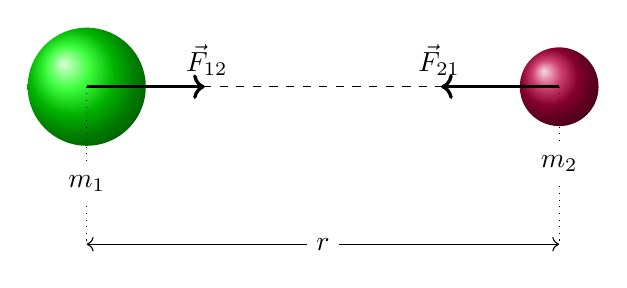
\begin{tikzpicture}
		\coordinate (A1) at (0,0);
		\coordinate (A2) at ($(A1)+(1.5cm,0)$);
		\coordinate (B1) at ($(A1)+(6cm,0)$);
		\coordinate (B2) at ($(B1)-(1.5cm,0)$);
		\shade[ball color=green] (A1) circle (0.75cm); 
		\shade[ball color=purple] (B1) circle (0.5cm);
		\draw[dashed] (A1) -- (B1);
		\draw[->,very thick] (A1)--(A2) node[near end,above right]{$\vec{F}_{12}$};
		\draw[->,very thick] (B1)--(B2) node[near end,above left]{$\vec{F}_{21}$};
		\coordinate (Ad) at ($(A1)-(0,2cm)$);
		\coordinate (Bd) at ($(B1)-(0,2cm)$);
		\draw[dotted] (A1) -- (Ad);
		\draw[dotted] (B1) -- (Bd);
		\draw[<->] (Ad) --(Bd);
		\node[below=1cm, fill=pagecol] at (A1) {$m_1$};
		\node[below=0.75cm, fill=pagecol] at (B1) {$m_2$};
		\node[fill=pagecol] at ($(Ad)!0.5!(Bd)$) {$r$};
	\end{tikzpicture}
\end{center}
Lực hấp dẫn giữa hai chất điểm bất kì tỉ lệ thuận với tích hai khối lượng của chúng và tỉ lệ nghịch với bình phương khoảng cách giữa chúng.
\begin{equation*}
	F_{\text {hd}} = G \dfrac {m_1 m_2 }{r^2},
\end{equation*}
trong đó:
\begin{itemize}
	\item $G$ là hằng số hấp dẫn, trong hệ SI có giá trị $G=\SI{6.67e-11}{\newton \meter ^2/\kilogram ^2}$;
	\item $m_1$, $m_2$ là khối lượng của hai vật;
	\item $r$ là khoảng cách giữa hai vật.
\end{itemize}

\subsubsection{Trọng lực }

Trọng lực là lực hấp dẫn của Trái Đất tác dụng vào vật gây ra cho chúng gia tốc rơi tự do. Trọng lực kí hiệu là $\vec P.$\\
Độ lớn của trọng lực:
\begin{equation*}
	P=F_{\text{hd}}=G \dfrac {mM}{(R+h)^2},
\end{equation*}
trong đó:
\begin{itemize}
	\item $m$ là khối lượng của vật ($\SI{}{\kilogram}$);
	\item $M$ là khối lượng Trái đất ($M \approx \SI{6e24}{\kilogram}$);
	\item $R$ là bán kính Trái đất ($R \approx \SI{6400e3}{\meter}$);
	\item $h$ là  độ cao của vật so với mặt đất ($\SI{}{\meter}$).
\end{itemize}

Gia tốc rơi tự do:
\begin{equation*}
	g=G \dfrac {M}{(R+h)^2}.
\end{equation*}
\begin{center}
	\includegraphics[scale=0.4]{../figs/VN10-PH-13-A-004-1-V2-01.jpg}
\end{center}
Ở gần Trái đất, trọng lực có phương thẳng đứng, có chiều từ trên xuống. \\
Công thức tính trọng lực: 
\begin{equation*}
	\vec P=m\vec g.
\end{equation*}

\subsubsection{Trọng lượng}
Khi vật đặt trong trọng trường và ở trạng thái cân bằng nhờ một dây treo hay giá đỡ, thì độ lớn của lực căng dây hoặc lực ép của vật lên giá đỡ gọi là trọng lượng của vật.  

\luuy{Không nên nhầm lẫn rằng trọng lượng là độ lớn của trọng lực. 
	
	Ví dụ, phi hành gia trên các trạm vũ trụ vẫn chịu tác dụng của trọng lực $P=mg$. Tuy nhiên nếu đặt một cái cân dưới chân phi hành gia thì cân chỉ số 0, vì trọng lực đã cân bằng với lực quán tính ly tâm (do trạm vũ trụ quay quanh Trái đất), nên phi hành gia không tạo được sức ép vào mặt cân. Ta nói phi hành gia ở trạng thái không trọng lượng (chứ không phải không trọng lực).}
\subsection{Lực căng dây}
\begin{minipage}[l]{0.5\textwidth}
	Khi kéo căng một sợi dây thì trong sợi dây xuất hiện lực căng chống lại xu hướng bị kéo dãn, gọi là lực căng dây. Lực căng dây kí hiệu là $\vec{T}$.

	Đối với dây không co giãn và khối lượng không đáng kể, độ lớn lực căng dây là như nhau tại mọi điểm trên dây. 
	
\end{minipage}
\begin{minipage}[r]{0.5\textwidth}
	\begin{center}
		\includegraphics[width=0.3\linewidth]{../figs/VN10-2023-PH-TP018-1}
		\captionof{figure}{Qủa cầu ở trạng thái cân bằng.}
	\end{center}
\end{minipage}
\section{Mục tiêu bài học - Ví dụ minh họa}
\begin{dang}{Ghi nhớ định luật vạn vật hấp dẫn. \\Nhận biết được đặc điểm của lực hấp dẫn}
	\viduii{1}{Lực hấp dẫn do một hòn đá ở trên mặt đất tác dụng vào Trái Đất thì có độ lớn
		\begin{mcq}(2)
			\item lớn hơn trọng lực của hòn đá.
			\item nhỏ hơn trọng lực của hòn đá.
			\item bằng trọng lực của hòn đá. 
			\item bằng 0.
		\end{mcq}
	}
	{\hide{
		Theo định luật III Newton: lực hấp dẫn do Trái Đất tác dụng lên hòn đá bằng lực hấp dẫn do hòn đá tác dụng lên Trái Đất.
		
		\textbf{Đáp án: C.}
	}}

	\viduii{1}{Chọn phát biểu sai về lực hấp dẫn giữa hai vật?
		\begin{mcq}
			\item Lực hấp dẫn tăng 4 lần khi khoảng cách giảm đi một nửa .
			\item Lực hấp dẫn không đổi khi khối lượng một vật tăng gấp đôi còn khối lượng vật kia giảm còn một nửa.
			\item Rất hiếm khi lực hấp dẫn là lực đẩy.
			\item Hằng số hấp dẫn có giá trị như nhau ở cả trên mặt Trái Đất và trên Mặt Trăng.
		\end{mcq}
		
	}
	{\hide{
		Lực hấp dẫn luôn là lực hút.
		
		\textbf{Đáp án: C.}
	}}
\end{dang}

\begin{dang}{Tính lực hấp dẫn và các đại lượng trong công thức của định luật vạn vật hấp dẫn}
	\viduii{3}{Cho biết khoảng cách giữa tâm Mặt Trăng và tâm Trái Đất là $\SI{38e7}{\meter}$; khối lượng Mặt Trăng và Trái Đất tương ứng là $\SI{7.37e22}{\kilogram}$ và $\SI{6e24}{\kilogram}$; hằng số hấp dẫn $G = \SI{6.67e-11}{\newton \meter ^2 / \kilogram ^2}$. Lực hấp dẫn giữa Trái Đất và Mặt Trăng có độ lớn là
		\begin{mcq}(2)
			\item $\SI{0.204e21}{\newton}$.
			\item $\SI{2.04e21}{\newton}$.
			\item $\SI{22e2}{\newton}$.
			\item $\SI{2e27}{\newton}$.
		\end{mcq}
	}
	{\hide{
		Áp dụng công thức lực hấp dẫn giữa Trái Đất và Mặt Trăng
		$$	F_{\text{hd}}=G\dfrac {m_1 m_2}{r^2} = \SI{0.204e21}{\newton}.$$
		
		\textbf{Đáp án: A.}
		
	}}

	\viduii{3}{Hai quả cầu giống nhau được đặt sao cho hai tâm cách nhau khoảng $r$ thì lực hấp dẫn giữa chúng là $F$. Nếu thay một trong hai khối cầu trên bằng một khối cầu đồng chất khác nhưng có bán kính lớn gấp hai, vẫn giữ nguyên khoảng cách giữa hai tâm (hai khối cầu không chạm nhau) thì lực hấp dẫn giữa chúng lúc này là
		\begin{mcq}(4)
			\item $2F$.
			\item $4F$.
			\item $8F$.
			\item $16F$.
		\end{mcq}
		
	}
	{\hide{
		Gọi quả cầu 2 là quả cầu có bán kính tăng gấp đôi. Bán kính của quả cầu 2 lúc sau
		$$r_2 ' = 2 r_2.$$
		
		Nếu $D$ là khối lượng riêng của quả cầu thì khối lượng của quả cầu 2 lúc sau sẽ là 
		$$m_2 ' = D V_2 ' = D\cdot \dfrac{4}{3}\pi {r'}_2^3= D\cdot \dfrac {4}{3} \pi (2r_2) ^3 = 8 D\cdot \dfrac {4}{3}\pi r_2 ^3 = 8 D V_2 = 8 m_2. $$
		
		Lực hấp dẫn giữa hai quả cầu lúc sau
		$$F_\text{hd}' = G \dfrac{m_1 m_2 '}{r^2} = 8 G \dfrac {m_1 m_2}{r^2} = 8F.$$
		
		\textbf{Đáp án: C.}
	}}
\end{dang}
\begin{dang}{Tính gia tốc rơi tự do và  trọng lượng vật trong các điều kiện khác nhau}
	\viduii{3}{Ở độ cao nào so với mặt đất thì gia tốc rơi tự do bằng một nửa gia tốc rơi tự do ở mặt đất? Cho bán kính Trái Đất là $R=\SI{6400}{\kilo \meter}$.
	}
	{\hide{
		Gia tốc rơi tự do ở mặt đất:
		$$g_0 = G \dfrac {M}{R^2}.$$
		
		Gia tốc rơi tự do ở độ cao $h$:
		$$g=G \dfrac {M}{(R+h)^2}.$$
		
		Gia tốc rơi tự do ở độ cao $h$ bằng một nửa gia tốc rơi tự do ở mặt đất, nên
		$$g=\dfrac{g_0}{2} \Rightarrow G \dfrac {M}{(R+h)^2} = G \dfrac {M}{2R^2} \Rightarrow (R+h)^2 = 2 R^2 \Rightarrow h=\SI{2650}{\kilo \meter}.$$
		
		Vậy ở độ cao $h=\SI{2650}{\kilo \meter}$ so với mặt đất thì gia tốc rơi tự do bằng một nửa so với gia tốc rơi tự do ở mặt đất.
		
	}}

	\viduii{3}{Tính độ cao mà ở đó gia tốc rơi tự do là 9,6 m/s$^2$. Biết bán kính Trái Đất là 6400 km và gia tốc rơi tự do ở sát mặt đất là 9,8 m/s$^2$.
	}
	{\hide{
		Gia tốc rơi tự do ở độ cao $h$ 
		\begin{equation*}
			g = \dfrac{GM}{(R+h)^2} = \text{9,6}\ \text{m/s}^2.
		\end{equation*}
		Gia tốc rơi tự do ở sát mặt đất 
		\begin{equation*}
			g_0 = \dfrac{GM}{R^2} = \text{9,8}\ \text{m/s}^2.
		\end{equation*}
		Suy ra 
		\begin{equation*}
			\dfrac{g}{g_0}= \left(\dfrac{R}{R+h}\right)^2 =\text{0,98}\Rightarrow h = \dfrac{R(1- \sqrt{\text{0,98}})}{\sqrt {\text{0,98}}} = 65\ \text{km}.
		\end{equation*}
		
	}}
\end{dang}
\begin{dang}{Mô tả được bằng ví dụ thực tiễn và biểu diễn được bằng hình vẽ: trọng lực, lực căng dây}
	\viduii{2}
	{Một bóng đèn có khối lượng $\SI{500}{\gram}$ được treo thẳng đứng vào trần nhà bằng một sợi dây và đang ở trạng thái cân bằng.
		\begin{enumerate}[label=\alph*)]
			\item Biểu diễn các lực tác dụng lên bóng đèn.
			\item Tính độ lớn của lực căng dây.
			\item Nếu dây treo chỉ chịu được một lực căng giới hạn $\SI{5.5}{\newton}$ thì nó có bị đứt không?
		\end{enumerate}
}
{\hide{
\begin{enumerate}[label=\alph*)]
\begin{minipage}[l]{0.6\textwidth}
\item Các lực tác dụng lên bóng đèn gồm:
	\begin{itemize}
		\item Trọng lực phương thẳng đứng hướng xuống.
		\item Lực căng dây phương thẳng đứng hướng lên.
	\end{itemize}
\item Vì bóng đèn đang ở trạng thái cân bằng nên:
$$T=P=mg=\left(\SI{0.5}{\kilogram}\right)\cdot\left(\SI{9.8}{\meter/\second^2}\right)=\SI{4.9}{\newton}$$
\item Dây không bị đứt vì lực căng mà dây phải chịu là $\SI{4.9}{\newton}$ nhỏ hơn lực căng giới hạn.
\end{minipage}
\begin{minipage}{0.4\textwidth}
	\begin{center}
		\includegraphics[width=0.3\linewidth]{../figs/VN10-2023-PH-TP018-2}
	\end{center}
\end{minipage}
\end{enumerate}
}}
\end{dang}
\begin{dang}{Tính các lực tác dụng lên vật \\khi vật cân bằng}
	\viduii{3}{Một vật có trọng lượng $P= 10$ N. được treo vào một vòng nhẫn O (coi là chất điểm). Vòng nhẫn được giữ yên bằng hai dây OA và OB. Biết dây OA nằm ngang và hợp với dây OB một góc $120^\circ.$ Tìm lực căng dây của hai dây OA và OB.
		
		\begin{center}
			\includegraphics[scale=0.5]{../figs/VN10-PH-11-L-008-4-V2-01.jpg}
		\end{center}
	}
	{\hide{
		\textbf{Cách 1: Áp dụng quy tắc tổng hợp lực.}
		\begin{center}
			\includegraphics[scale=0.8]{../figs/VN10-PH-11-L-008-4-V2-02.jpg}
		\end{center}
		Khi vật ở vị trí cân bằng thì các lực tác dụng lên vật gồm trọng lực $\vec{P}$, lực căng trên hai dây $\vec{T}_A$ và $\vec{T}_B$. Vòng nhẫn đứng yên nên các lực cân bằng nhau
		$$\vec{P}+\vec{T}_\textrm{A}+\vec{T}_\textrm{B}=\vec{0}.$$
		Gọi $\vec{Q}$ là hợp lực của $\vec{P}$ và $\vec{T}_A$
		$$\vec{P}+\vec{T}_\textrm{A}=\vec{Q}\quad\Rightarrow \quad\vec{T}_\textrm{B}+\vec{Q}=\vec{0}\quad\Rightarrow\quad \vec{T}_\textrm{B}=-\vec{Q}$$
		nghĩa là $\vec{Q}$ và $\vec{T}_B$ là hai vector trực đối. Do đó, $\alpha =\SI{	180}{\degree}-\SI{120}{\degree}=\SI{60}{\degree}.$
		
		Xét $\triangle$O$T_\text{A}$Q vuông tại $T_\text{A}$:
		
		$$\tan \alpha =\dfrac{P}{T_\text{A}}\Rightarrow T_\text{A}=\dfrac{P}{\tan \alpha}=\dfrac{10\sqrt{3}}{3}\,\text{N}.$$
		$$\sin \alpha =\dfrac{P}{Q}\Rightarrow Q=\dfrac{P}{\sin \alpha}=\dfrac{20\sqrt{3}}{3}\,\text{N}.$$
		Vì $|\vec{T}_\textrm{B}|=|\vec{Q}|$ nên $T_\textrm{B}= \dfrac{20\sqrt{3}}{3}\,\text{N}.$
		
		Vậy lực căng dây của hai dây OA và OB lần lượt bằng $\dfrac{10\sqrt{3}}{3}\,\text{N}, \dfrac{20\sqrt{3}}{3}\,\text{N}.$\\
		\textbf{Cách 2: Áp dụng quy tắc tam giác lực}\\
		Vòng nhẫn đứng yên nên các lực cân bằng nhau
		$$\vec{P}+\vec{T}_\textrm{A}+\vec{T}_\textrm{B}=\vec{0}.$$
		Do đó, $\left(\vec{P}, \overrightarrow{T_A}, \overrightarrow{T_B}\right)$ tạo thành tam giác khép kín
		\begin{center}
			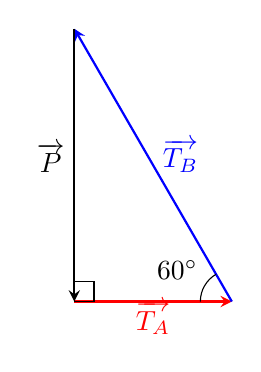
\begin{tikzpicture}
				\coordinate (O) at (2,0);
				\coordinate (A) at (0,0);
				\coordinate (B) at (0,3.464);
				\coordinate (O1) at (1,0);
				\coordinate (A1) at (1,1.73);
				\coordinate (B1) at (0,1.7);
				\draw[-stealth,thick, red] (A) -- (O);
				\draw[-stealth,thick, blue] (O) -- (B);
				\draw[-stealth,thick] (B) -- (A);
				\node[label={[red,below]90:$\overrightarrow{T_A}$}] at (O1){};	
				\node[label={[blue,right]90:$\overrightarrow{T_B}$}] at (A1){};	
				\node[label={[black,left]90:$\overrightarrow{P}$}] at (B1){};	
				\tkzMarkAngle[size=0.4,color=black](B,O,A);
				\tkzLabelAngle[color=black,pos=0.8](B,O,A){$\SI{60}{\degree}$}
				\tkzMarkRightAngle[draw=black,size=.25](B,A,O);
			\end{tikzpicture}
		\end{center}
		Từ tam giác vectơ ta xác định được 
		\begin{align*}
			\begin{cases}
				T_A=\dfrac{P}{\tan\SI{60}{\degree}}=\xsi{\dfrac{10\sqrt{3}}{3}}{\newton}\\
				T_B=\dfrac{P}{\sin\SI{60}{\degree}}=\xsi{\dfrac{20\sqrt{3}}{3}}{\newton}
			\end{cases}
		\end{align*}
		
	}}

	\viduii{3}{Một đèn tín hiệu giao thông ở đại lộ có trọng 
		lượng 120 N được treo vào trung điểm của dây 
		AB làm dây thòng xuống $\text{0,5}$ m. Cho biết hai trụ treo dây cách nhau \SI{8}{\meter}, bỏ qua 
		trọng lượng của dây, tính lực căng mỗi sợi dây. 
		\begin{center}
			\includegraphics[scale=0.7]{../figs/VN10-PH-11-L-008-4-V2-03.jpg}
		\end{center}
	}
	{\hide{
		\textbf{Cách 1: Phân tích lực.}
		\begin{center}
			\includegraphics[scale=0.5]{../figs/VN10-PH-11-L-008-4-V2-04.jpg}
		\end{center}
		Đèn khi cân bằng chịu các lực tác dụng như hình vẽ, gồm trọng lực $\vec{P}$, hai lực căng dây $\vec{T}_1$ và $\vec{T}_2$
		\begin{align*}
			\vec{P}+\vec{T}_1+\vec{T}_2=0
		\end{align*}
		
		Gọi $\vec T$ là hợp lực của hai dây cáp:
		$$\vec{T}=\vec{T}_1+\vec{T}_2\quad\Rightarrow\quad \vec{P}+\vec{T}=0$$
		nghĩa là $T=P=mg=\SI{120}{\newton}$.
		
		Do tính đối xứng, hai lực căng dây phải có độ lớn bằng nhau $T_1=T_2$. Từ hình vẽ 
		\begin{align*}
			T=2T_1\cos \alpha\quad\Rightarrow\quad T_1=\dfrac{T}{2\cos\alpha}
		\end{align*}
		trong đó góc $\alpha$ được xác định từ tam giác vuông bên phải trên hình
		\begin{align*}
			\tan\alpha=\dfrac{\SI{4}{\meter}}{\SI{0.5}{\meter}}=8\quad\Rightarrow\quad \alpha\approx\SI{82.875}{\degree}. 
		\end{align*}
		Từ đó ta tính được lực căng dây
		\begin{align*}
			T_1=T_2=\dfrac{T}{2\cos\alpha}\approx \SI{484}{\newton}.
		\end{align*}		
	\textbf{Cách 2: Dùng tam giác lực}\\
	Đèn cân bằng nên
	\begin{align*}
		\vec{P}+\vec{T}_1+\vec{T}_2=\overrightarrow{0}
	\end{align*}
Do tính đối xứng, hai lực căng dây phải có độ lớn bằng nhau $T_1=T_2$.\\
Ba vectơ lực $\vec{P}, \overrightarrow{T_1}, \overrightarrow{T_2}$ tạo thành tam giác vectơ khép kín
	\begin{center}
	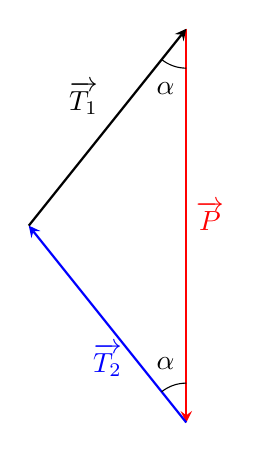
\begin{tikzpicture}
		\coordinate (O) at (0,0);
		\coordinate (A) at (0,-5);
		\coordinate (B) at (-2,-2.5);
		\coordinate (O1) at (0,-2.5);
		\coordinate (A1) at (-1,-4);
		\coordinate (B1) at (-1,-1);
		\draw[-stealth,thick, red] (O) -- (A);
		\draw[-stealth,thick, blue] (A) -- (B);
		\draw[-stealth,thick] (B) -- (O);
		\node[label={[red,right]90:$\overrightarrow{P}$}] at (O1){};	
		\node[label={[blue,below]90:$\overrightarrow{T_2}$}] at (A1){};	
		\node[label={[black,left]90:$\overrightarrow{T_1}$}] at (B1){};	
		\tkzMarkAngle[size=0.5,color=black](O,A,B);
		\tkzLabelAngle[color=black,pos=0.8](O,A,B){$\alpha$};
		\tkzMarkAngle[size=0.5,color=black](B,O,A);
		\tkzLabelAngle[color=black,pos=0.8](B,O,A){$\alpha$}
	\end{tikzpicture}
\end{center}
Áp dụng định lý hàm sin:
\begin{align*}
	\dfrac{T_1}{\sin\alpha}&=\dfrac{P}{\sin\left(\SI{180}{\degree}-2\alpha\right)}\Leftrightarrow \dfrac{T_1}{\sin\alpha}=\dfrac{P}{\sin\left[2\cdot\left(\SI{90}{\degree}-\alpha\right)\right]}\\
	\Rightarrow \dfrac{T_1}{\sin\alpha}&=\dfrac{P}{2\sin\left(\SI{90}{\degree}-\alpha\right)\cos\left(\SI{90}{\degree}-\alpha\right)}=\dfrac{P}{2\cos\alpha\sin\alpha}\\
	\Rightarrow T_1&=\dfrac{P}{2\cos\alpha}\approx\SI{484}{\newton}
\end{align*}
	}}
	
	
\end{dang}
%				\let\lesson\undefined
\newcommand{\lesson}{\phantomlesson{Bài 11.}}
\setcounter{section}{2}
\section{Bài tập trắc nghiệm}
\begin{enumerate}[label=\bfseries Câu \arabic*:,leftmargin=1.5cm]
	\item \mkstar{1}\\
	{Phát biểu nào sau đây là đúng khi nói về phương, chiều của trọng lực?
		\begin{mcq}
			\item Trọng lực có phương nằm ngang và có chiều hướng về phía Trái Đất.
			\item Trọng lực có phương thẳng đứng và có chiều hướng ra xa Trái Đất.
			\item Trọng lực có phương nằm ngang và có chiều hướng ra xa Trái Đất.
			\item Trọng lực có phương thẳng đứng và có chiều hướng về tâm Trái Đất.
		\end{mcq}
	
}
\hideall{
\textbf{Đáp án: D.}
}

\item\mkstar{1}\\
{Một vật có khối lượng $\SI{500}{\gram}$, trọng lượng của nó có giá trị gần đúng là
	\begin{mcq}(4)
		\item $\SI{5}{\newton}$.
		\item $\SI{50}{\newton}$.
		\item $\SI{500}{\newton}$.
		\item $\SI{5000}{\newton}$.
	\end{mcq}

}
\hideall{
\textbf{Đáp án: A.}
}

\item \mkstar{2}\\
{Trang phục của các nhà du hành vũ trụ có khối lượng khoảng 50 kg. Tại sao họ vẫn có thể di chuyển dễ dàng trên Mặt Trăng?
	\begin{mcq}
		\item Vì mọi vật trên Mặt Trăng đều chịu lực hấp dẫn lớn hơn nhiều lần so với trên Trái Đất.
		\item Vì mọi vật trên Mặt Trăng đều chịu lực hấp dẫn nhỏ hơn nhiều lần so với trên Trái Đất.
		\item Vì mọi vật trên Mặt Trăng đều không chịu lực hấp dẫn.
		\item Vì mọi vật trên Trái Đất đều không chịu lực hấp dẫn.
	\end{mcq}

}
\hideall{
\textbf{Đáp án: B.}
}

\item \mkstar{2}\\
{Một vật có khối lượng $m$ đặt ở nơi có gia tốc trọng trường $g$. Phát biểu nào sau đây sai?
\begin{mcq}
	\item Trọng lực có độ lớn được xác định bởi biểu thức $P = mg$.
	\item Điểm đặt của trọng lực là trọng tâm của vật.
	\item Trọng lực tỉ lệ nghịch với khối lượng của vật.
	\item Trọng lực là lực hút của Trái Đất tác dụng lên vật.
\end{mcq}
}
\hideall{
\textbf{Đáp án: C.}
}

\item\mkstar{2}\\
{Điều nào sau đây đúng khi nói về lực căng dây?
	\begin{mcq}
		\item Lực căng dây có phương dọc theo dây, chiều chống lại xu hướng bị kéo dãn.
		\item Lực căng dây có phương dọc theo dây, cùng chiều với lực do vật kéo dãn dây.
		\item Với những dây có khối lượng không đáng kể thì lực căng ở hai đầu dây luôn có cùng một độ lớn.
		\item Với nhưng dây có khối lượng không đáng kể thì lực căng ở hai đâu dây luôn khác nhau về độ lớn.
	\end{mcq}

}
\hideall{
\textbf{Đáp án: A.}
}

\item\mkstar{2}\\
{Một vật đang nằm yên trên mặt đất, lực hấp dẫn do Trái Đất tác dụng vào vật có độ lớn
	\begin{mcq}(2)
		\item lớn hơn trọng lượng của vật.
		\item nhỏ hơn trọng lượng của vật.
		\item bằng trọng lượng của vật.
		\item bằng 0.
	\end{mcq}

}

\item\mkstar{2}\\
{Tại cùng một địa điểm, hai vật có khối lượng $m_1<m_2$, trọng lực tác dụng lên hai vật lần lượt là $P_1$ và $P_2$ luôn thoả mãn điều kiện
	\begin{mcq}(4)
		\item $P_1=P_2$.
		\item $\dfrac{P_1}{P_2}<\dfrac{m_1}{m_2}$.
		\item $P_1>P_2$.
		\item $\dfrac{P_1}{P_2}=\dfrac{m_1}{m_2}$.
	\end{mcq}

}
\hideall{
\textbf{Đáp án: D.}
}

\item\mkstar{2}\\
{Biết gia tốc rơi tự do ở đỉnh và ở chân một ngọn núi lần lượt là $\SI{9.809}{\meter/\second^2}$ và $\SI{9.810}{\meter/\second^2}$. Tỉ số trọng lượng của vật ở đỉnh núi và chân núi là
	\begin{mcq}(4)
		\item 0,9999.
		\item 1,0001.
		\item 9,8095.
		\item 0,0005.
	\end{mcq}

}
\hideall{
\textbf{Đáp án: A.}
}

\item \mkstar{3}\\
{Một người đi chợ dùng lực kế để kiểm tra khối lượng của một gói hàng. Người đó treo gói hàng vào lực kế và đọc được số chỉ của lực kế là $\SI{20}{\newton}$. Biết gia tốc rơi tự do tại vị trí này là $\SI{10}{\meter/\second^2}$. Khối lượng của túi hàng là
	\begin{mcq}(4)
		\item $\SI{2}{\kilogram}$.
		\item $\SI{20}{\kilogram}$.
		\item $\SI{30}{\kilogram}$.
		\item $\SI{10}{\kilogram}$.
	\end{mcq}

}
\hideall{
\textbf{Đáp án: A.}
}

\item\mkstar{3}\\
{Một ngọn đèn có khối lượng $m=\SI{1}{\kilogram}$ được treo dưới trần nhà bằng một sợi dây. Lấy $g=\SI{9.8}{\meter/\second^2}$. Dây chỉ chịu được lực căng lớn nhất là $\SI{8}{\newton}$. Nếu treo ngọn đèn này vào một đầu dây thì
	\begin{mcq}(2)
		\item lực căng sợi dây là $\SI{9}{\newton}$ và sợi dây sẽ bị đứt.
		\item lực căng sợi dây là $\SI{9.8}{\newton}$ và sợi dây sẽ bị đứt.
		\item lực căng sợi dây là $\SI{9.8}{\newton}$ và sợi dây không bị đứt.
		\item lực căng sợi dây là $\SI{4.9}{\newton}$ và sợi dây không bị đứt.
	\end{mcq}

}
\hideall{
\textbf{Đáp án: B.}
}
\end{enumerate}
\section{Bài tập tự luận}
\begin{enumerate}[label=\bfseries Bài \arabic*:,leftmargin=1.5cm]
	\item \mkstar{2}
	
	
	{Hãy chỉ ra điểm đặt, phương, chiều của lực căng trong hình a, b.
		\begin{center}
			\includegraphics[scale=1]{../figs/VN10-2022-PH-TP019-3.jpg}
		\end{center}
	}
	
	\hideall
	{
		Xác định điểm đặt, phương, chiều của lực căng trong:
		
		- Hình a:
		
		+ Điểm đặt: tại 2 đầu sợi dây.
		
		+ Phương: trùng với phương của sợi dây.
		
		+ Chiều: ngược với chiều của lực do người kéo dãn dây.
		
		- Hình b:
		
		+ Điểm đặt: tại vật.
		
		+ Phương: trùng với phương của sợi dây.
		
		+ Chiều: ngược với chiều của lực do người kéo dãn dây.
		
	}
	\item \mkstar{3}
	
	{
		Lực kế trong hình đang chỉ ở vạch $\SI{10}{N}$.
		\begin{center}
			\includegraphics[scale=0.8]{../figs/VN10-2022-PH-TP019-1.jpg}
		\end{center}
		Tính trọng lượng và khối lượng của vật treo vào lực kế. Lấy $g \approx \SI{9,8}{m/s}^2$.
		
		
	}
	
	\hideall{
		
		Trọng lượng của vật là $\SI{10}{N}$. Khối lượng của vật là :
		
		$$m= \dfrac{P}{g} = \SI{1,02}{kg}.$$
		
		Vật chịu tác dụng bởi 2 lực cùng phương là lực hút trái đất có chiều từ trên xuống và lức kéo của lò xo có chiều từ dưới lên. 
		
	}
	
	\item \mkstar{3}
	
	
	{Đo trọng lượng của một vật ở một địa điểm trên Trái Đất có gia tốc rơi tự do là $\SI{9,8}{m/s}^2$, ta được $P = \SI{9,8}{N}$. Nếu đem vật này tới một địa điểm khác có gia tốc rơi tự do $\SI{9,78}{m/s}^2$ thì khối lượng và trọng lượng của nó đo được là bao nhiêu?
	}
	
	\hideall
	{
		Khối lượng của vật là
		
		$$ m = \dfrac{P}{g} = \SI{1}{kg}.$$
		
		Trọng lượng của vật ở nơi có gia tốc $\SI{9,78}{m/s}^2$ là
		
		$$P= mg = \SI{9,78}{N}.$$
	}
	\item \mkstar{3}
	
	
	{Một bóng đèn có khối lượng $\SI{500}{g}$ được treo thẳng đứng vào trần nhà bằng một sợi dây và đang ở trạng thái cân bằng.
		\begin{enumerate}[label=\alph*)]
			\item Biểu diễn các lực tác dụng lên bóng đèn.
			\item Tính độ lớn của lực căng. 
			\item Nếu dây treo chỉ chịu được một lực căng giới hạn $\SI{5,5}{N}$ thì nó có bị đứt không?
		\end{enumerate}
		
	}
	
	\hideall
	{
		\begin{enumerate}[label=\alph*)]
			\item Các lực tác dụng là: Lực hút của trái đất có chiều từ trên xuống và lực kéo của dây treo có chiều tư dưới lên, và chúng cùng phương.
			
			\item Độ lớn của lực căng dây 
			
			$$P= mg = \SI{4,9}{N}.$$
			
			\item 
			
			Nếu dây treo chỉ chịu được một lực căng giới hạn $\SI{5,5}{N}$, thì nó không bị đứt vì lực kéo của dây vẫn nhỏ hơn lực căng giới hạn.
		\end{enumerate}
	}
	\item \mkstar{3}
	
	
	{Một con khỉ biểu diễn xiếc treo mình cân bằng trên một sợi dây bằng một tay như hình. Hãy cho biết trong hai lực căng xuất hiện trên dây ($\vec T_1$ và $\vec T_2$), lực nào có cường độ lớn hơn? Tại sao?
		\begin{center}
			\includegraphics[scale=1]{../figs/VN10-2022-PH-TP019-2.jpg}
		\end{center}
	}
	
	\hideall
	{Con khỉ cân bằng:
		$$\overrightarrow{P}+\overrightarrow{T_1}+\overrightarrow{T_2}=\overrightarrow{0}$$
		Chiếu lên phương nằm ngang:
		$$T_1\cos\SI{14}{\degree}=T_2\cos\SI{20}{\degree}\Rightarrow T_1\approx0,97T_2$$
		Vậy $T_2>T_1$.
	}
	
	\item \mkstar{4}
	
	
	{
		Vật rắn $\SI{2}{kg}$ nằm cân bằng trên mặt phẳng nghiêng góc $30^\circ$. Lực căng dây có giá trị là bao nhiêu? Lấy $g=\SI{9,8}{m/s}^2$ và bỏ qua ma sát.
		\begin{center}
			\includegraphics[scale=1]{../figs/VN10-2022-PH-TP019-5.jpg}
		\end{center}
	}
	
	\hideall
	{
		\begin{center}
			\includegraphics[scale=0.5]{../figs/VN10-2022-PH-TP019-4.jpg}
		\end{center}
		
		+ Các lực tác dụng lên vật gồm: trọng lực $P$, lực căng dây $T$, phản lực $N$.
		
		+ Ta có:
		
		$$\vec P + \vec T + \vec N = \vec 0\ (1).$$
		
		+ Gắn hệ trục tọa độ, chiếu (1) theo phương Ox, ta được:
		
		$$-T + P_\text{x} = 0 \Rightarrow T = P_\text{x} = P\sin \alpha = mg \sin \alpha = \SI{9,8}{N}.$$
		\textit{Có thể dùng tam giác vector để giải.}
		
	}
	\item \mkstar{4}
	
	
	{
		Một vật rắn khối lượng $\SI{5}{kg}$ được treo cân bằng trên mặt phẳng thẳng đứng bằng một sợi dây như hình vẽ. Bỏ qua ma sát, lấy $g=\SI{9,8}{m/s}^2$; $\alpha = 20^\circ$. Vậy lực căng dây là bao nhiêu?
		\begin{center}
			\includegraphics[scale=0.8]{../figs/VN10-2022-PH-TP019-6.jpg}
		\end{center}
	}
	
	\hideall
	{
		\begin{center}
			\includegraphics[scale=0.8]{../figs/VN10-2022-PH-TP019-7.jpg}
		\end{center}
		Các lực tác dụng lên vật gồm: trọng lực $P$, lực căng dây $T$ và phản lực $R$ của mặt phẳng thẳng đứng.
		
		Ta có:
		
		$$\vec P + \vec T + \vec N = \vec 0\ (1).$$
		
		Chọn hệ trục Oxy như hình, chiếu (1) theo các phương, ta được:
		
		$$ - P + T\cos \alpha = 0 \Rightarrow T = \dfrac{P}{\cos \alpha} = \SI{52,14}{N}.$$
	}
	\item \mkstar{4}
	
	
	{
		Treo một vật nặng khối lượng $\SI{6}{kg}$ vào điểm giữa của một sợi dây cáp căng ngang giữa hai cột thẳng đứng cách nhau $\SI{8}{m}$ làm dây võng xuống $\SI{0,5}{m}$. Lấy $g=\SI{10}{m/s}^2$. Tính lực căng của dây.
	}
	
	\hideall
	{
		\begin{center}
			\includegraphics[scale=0.8]{../figs/VN10-2022-PH-TP019-10.jpg}
		\end{center}
		
		Theo đề bài ta có:
		
		$$T = T'; \text{IH} = \SI{0,5}{m}; \text{HA} = \SI{4}{m}.$$
		
		Vật cân bằng:
		
		$$\vec P + \vec T + \vec T' = \vec 0.$$
		
		Từ hình ta có:
		
		$$P = 2T \sin \alpha.$$
		
		Mặt khác, ta có:
		
		$$\tan \alpha = \dfrac{\text{IH}}{\text{HA}} = \dfrac{1}{8} \Rightarrow \sin \alpha = \text{0,124} \Rightarrow T = \dfrac{P}{2\sin \alpha} = \SI{241,9}{N}.$$
	}
	\item \mkstar{4}
	
	
	{
		Vật rắn nằm cân bằng như hình vẽ, góc hợp bởi lực căng của dây là $150^\circ$. Tính trọng lượng của vật biết độ lớn lực căng của hai dây là $\SI{200}{N}$.
		\begin{center}
			\includegraphics[scale=0.8]{../figs/VN10-2022-PH-TP019-8.jpg}
		\end{center}
	}
	
	\hideall
	{
		\begin{center}
			\includegraphics[scale=0.8]{../figs/VN10-2022-PH-TP019-9.jpg}
		\end{center}
		
		Ta có: 
		
		$$T_1 = T_2 = T = \SI{200}{N}.$$
		
		Vật nằm cân bằng nên:
		
		$$\vec T_1 + \vec T_2 + \vec P = \vec 0.$$
		
		Suy ra: 
		
		$$P = T_{12} = 2T \cos \dfrac{\alpha}{2} \approx \SI{103,5}{N}.$$
		
		
	}
	
	\item \mkstar{4}
	
	{ Một vật có trọng lượng $\SI{60}{\newton}$ được treo vào vòng nhẫn nhẹ O (coi là chất điểm). Vòng nhẫn được giữ bằng hai dây nhẹ OA và OB. Biết OA nằm ngang còn OB hợp với phương thẳng đứng góc $45^\circ$ (hình vẽ). Tìm lực căng của dây OA và OB.
		\begin{center}
			\includegraphics[scale=0.8]{../figs/VN10-2021-PH-TP011-1.jpg}
		\end{center}
	}
	\hideall{
		
		\begin{center}
			\includegraphics[scale=0.8]{../figs/VN10-2021-PH-TP011-2.jpg}
		\end{center}
		
		Các lực tác dụng vào điểm treo O như hình vẽ.
		
		Góc $\alpha$ là góc giữa OP và OB, $\alpha=45^\circ$.
		$$\text{OI}=\text{OK}\cdot \cos \alpha\Rightarrow \text{OK}=\dfrac{\text{OI}}{\cos \alpha}\Rightarrow T_\text{OB}=\dfrac{P}{\cos \alpha}=60\sqrt{2}\ \text{N} $$.
		
		Tương tự:   $$T_\text{OA}=T_\text{OB}\cdot \sin 45^\circ=60\ \text{N}$$
	}
\end{enumerate}
%				\let\lesson\undefined
\newcommand{\lesson}{\phantomlesson{Bài 12: Một số lực trong thực tiễn}}
\chapter[Lực ma sát]{Lực ma sát}
\setcounter{section}{0}
\section{Lý thuyết}
\subsection{Lực ma sát nghỉ}
\subsubsection{Định nghĩa}
Lực ma sát nghỉ xuất hiện ở mặt tiếp xúc khi một vật nằm yên trên bề mặt vật khác và có xu hướng chuyển động dưới tác dụng của ngoại lực.
\begin{center}
	\includegraphics[width=0.4\linewidth]{../figs/VN10-2023-PH-TP019-1}
	\captionof{figure}{Thùng gỗ bất động khi bị người đẩy.}
\end{center}
\subsubsection{Đặc điểm}
\begin{itemize} 
	\item Điểm đặt: trên vật và ngay tại vị trí tiếp xúc của hai bề mặt, 
	\item Phương: tiếp tuyến với bề mặt tiếp xúc,
	\item Chiều: ngược chiều xu hướng chuyển động tương đối của hai bề mặt tiếp xúc,
	\item Độ lớn: bằng độ lớn của lực tác dụng gây ra xu hướng chuyển động.
\end{itemize}
\luuy{Điều kiện để vật trượt 
$$F\ge F_{msn\ \text{max}}=\mu_N\cdot N$$
trong đó:
\begin{itemize}
	\item $F_{msn\ \text{max}}$: lực ma sát nghỉ cực đại;
	\item $\mu_N$: hệ số ma sát nghỉ;
	\item $N$: áp lực do vật tác dụng lên bề mặt tiếp xúc.
\end{itemize}
Lực ma sát nghỉ cực đại lớn hơn ma sát trượt.
}
\subsection{Lực ma sát trượt}
\subsubsection{Định nghĩa}
Lực ma sát trượt xuất hiện ở mặt tiếp xúc khi một vật trượt trên một bề mặt và cản trở lại chuyển động trượt của vật đó.
\begin{center}
	\includegraphics[scale=0.35]{../figs/VN10-PH-15-L-012-1-V2-01.JPG}
\end{center}
\subsubsection{Đặc điểm}
\begin{itemize}
	\item Điểm đặt: trên vật và ngay tại vị trí tiếp xúc của hai bề mặt,
	\item Phương: tiếp tuyến với mặt tiếp xúc giữa 2 vật trượt,
	\item Chiều: ngược chiều với vận tốc tương đối của vật ấy đối với vật kia,
	\item Độ lớn:
	\begin{itemize}
		\item không phụ thuộc vào diện tích tiếp xúc và tốc độ của vật.
		\item tỉ lệ với độ lớn của áp lực.
		\item phụ thuộc vào vật liệu và tình trạng của hai mặt tiếp xúc.
	\end{itemize}
	\item Biểu thức 
	\begin{equation*}
		F_{\text{mst}} = \mu_{\text{t}} \cdot N,
	\end{equation*}
	trong đó:
	
	+ $\mu_{\text{t}}$ là hệ số ma sát trượt, nó phụ thuộc vào bản chất của hai mặt tiếp xúc và các điều kiện trên bề mặt (không có đơn vị),
	
	+ $N$ là áp lực của vật lên mặt tiếp xúc.
\end{itemize}
\subsubsection{Vai trò}
\begin{itemize}
	\item Ma sát trượt có ích trong việc mài dũa, thắng xe, \dots
	\item Ma sát trượt có hại trong các ổ trục trượt, mài mòn xilanh, pittông xe, \dots Để giảm ma sát trượt, người ta bôi trơn các chi tiết bằng dầu mỡ công nghiệp.
\end{itemize}
\subsection{Lực ma sát lăn}
\begin{itemize}
	\item Lực ma sát lăn xuất hiện ở mặt tiếp xúc khi một vật lăn trên một bề mặt và cản trở lại chuyển động lăn của vật đó.
	\item Lực ma sát lăn có các đặc điểm giống như lực ma sát trượt nhưng hệ số ma sát lăn nhỏ hơn rất nhiều lần (hàng chục lần) hệ số ma sát trượt.
	\item Trong trường hợp lực ma sát trượt có hại, cần phải giảm thì người ta dùng con lăn hay ổ bi đặt xen vào giữa hai mặt tiếp xúc để giảm tổn hại vì ma sát.
\end{itemize}
\begin{center}
	\includegraphics[scale=0.25]{../figs/VN10-PH-15-L-012-1-V2-02.JPG}
\end{center}

\subsubsection{Vai trò}
\begin{itemize}
	\item Giúp ta cầm nắm được các vật, giữ vật ở yên tại vị trí đã định, dây cua roa truyền được chuyển động giữa các bánh xe, băng chuyền vận chuyển được người hoặc vật từ nơi này đến nơi khác...
	\item Đóng vai trò lực phát động, giúp sinh vật, xe cộ di chuyển được.
	\begin{center}
		\includegraphics[scale=0.35]{../figs/VN10-PH-15-L-012-1-V2-03.JPG}
		\captionof{figure}{Lực ma sát do mặt đất tác dụng lên chân người khi đi sẽ làm cho người có thể tiến về phía trước.}
	\end{center}
	\item Trong những trường hợp ma sát có lợi, người ta tìm cách tăng tính nhám của các mặt tiếp xúc và tăng áp lực lên mặt tiếp xúc, chẳng hạn thêm các rãnh trên đế giày, bánh xe để tăng ma sát.
\end{itemize}

\section{Mục tiêu bài học - Ví dụ minh họa}
\begin{dang}{Ghi nhớ khái niệm các loại lực ma sát}
	\viduii{1}{Hệ số ma sát trượt
		\begin{mcq}
			\item tỉ lệ thuận với lực ma sát trượt và tỉ lệ nghịch với áp lực. 
			\item phụ thuộc diện tích tiếp xúc và tốc độ của vật.
			\item phụ thuộc vào vật liệu và tình trạng của mặt tiếp xúc. 
			\item phụ thuộc vào áp lực.
		\end{mcq}
	}
	{\hide{
		Hệ số ma sát trượt phụ thuộc vào vật liệu và tình trạng của mặt tiếp xúc   
		
		\textbf{Đáp án: C}.
	}}

	\viduii{1}{Chiều của lực ma sát nghỉ
		\begin{mcq}
			\item  Ngược chiều với vận tốc của vật.
			\item  Ngược chiều với gia tốc của vật.
			\item  Ngược chiều với thành phần ngoại lực song song với mặt tiếp xúc.
			\item  Vuông góc với mặt tiếp xúc.
		\end{mcq}
	}
	{\hide{
		Chiều của lực ma sát nghỉ ngược chiều với thành phần ngoại lực song song với mặt tiếp xúc.
		
		\textbf{Đáp án: C}.
	}}


	\viduii{1}{Phát biểu nào sau đây là đúng khi nói về ma sát
		\begin{mcq}
			\item Lực ma sát lăn cản trở chuyển động của vật này trượt trên vật khác.
			\item Khi vật chuyển động chậm dần, lực ma sát nhỏ hơn lực đẩy.
			\item Lực ma sát lăn nhỏ hơn lực ma sát trượt.
			\item Khi vật chuyển động nhanh dần, lực ma sát lớn hơn lực đẩy.
		\end{mcq}
	}
	{\hide{
		A - sai vì: lực ma sát lăn cản trở chuyển động của vật này lăn trên vật khác
		
		B - sai vì: khi vật chuyển động chậm dần, lực ma sát lớn hơn lực đẩy
		
		C - đúng
		
		D - sai vì: khi vật chuyển động nhanh dần, lực ma sát nhỏ hơn lực đẩy
		
		\textbf{Đáp án: C}.
	}}
\end{dang}
\begin{dang}{Tính độ lớn lực ma sát và các đại lượng\\ trong công thức lực ma sát trượt}
	\viduii{2}{Một ô tô khối lượng 1,5 tấn chuyển động thẳng đều trên đường. Hệ số ma sát lăn giữa bánh xe và mặt đường là 0,08. Tính lực làm cản trở chuyển động của xe trên mặt đường (bỏ qua lực cản không khí).
	}
	{\hide{
		\manatip{Trong trường hợp xe chuyển động do lực đẩy của động cơ, ta xem như lực này có phương song song với mặt đất.}
		
		Lực đẩy song song với mặt ngang, nên phản lực có độ lớn bằng với trọng lực. Lực làm cản trở chuyển động của xe trên mặt đường là lực ma sát
		\begin{equation*}
			F_{\text{ms}} =\mu N = \mu  mg =\SI{0.08}{}\cdot(\SI{1.5e3}{\kilogram})\cdot\SI{9.81}{\meter/\second^{2}}\approx \SI{1177}{N}.
		\end{equation*}
		
		
	}}

	\viduii{2}{Một toa tàu có khối lượng 80 tấn chuyển động thẳng đều dưới tác dụng của lực kéo $F = 6\cdot 10^4\ \text{N}$. Xác định lực ma sát và hệ số ma sát giữa toa tàu với mặt đường
	}
	{\hide{
		Tàu chuyển động thẳng đều nên lực ma sát cân bằng với lực kéo của toa tàu
		\begin{equation*}
			F_{\text{ms}} = F_{\text{k}} = \mu mg.
		\end{equation*}
		Suy ra hệ số ma sát
		\begin{equation*}
			\mu = \dfrac{F_{\text{k}}}{mg} = \text{0,075}.
		\end{equation*} 
	}}

\end{dang}
\begin{dang}{Giải bài toán vật chuyển động trên mặt phẳng ngang có ma sát}
	\viduii{3}{Một ô tô khối lượng 1 tấn, chuyển động trên mặt đường nằm ngang. Hệ số ma sát lăn giữa xe và mặt đường là 0,1. Tính lực kéo của động cơ ô tô trong mỗi trường hợp sau
		
		a) Ô tô chuyển động thẳng đều.
		
		b) Ô tô chuyển động nhanh dần đều với gia tốc $a = \SI{2}{m/s}^2$, lấy $g=\SI{10}{m/s^2}$.
	}
	{\hide{
		\begin{center}
			\includegraphics[scale=0.6]{../figs/VN10-PH-15-A-005-3-V2-03.JPG}
		\end{center} 
		Áp dụng định luật II Newton
		\begin{equation*}
			\vec{N}+\vec{P} + \vec{F}_{\text{ms}} + \vec{F} = m\vec{a}.
		\end{equation*}
		Chiếu lên O$y$:
		\begin{equation*}
			N=P = mg.
		\end{equation*}
		Chiếu lên O$x$:
		\begin{equation*}
			F-F_{\text{ms}} = ma \Rightarrow F = ma + F_{\text{ms}}
		\end{equation*}
		a) Khi ô tô chuyển động thẳng đều thì $a=0$ nên lực kéo của ô tô đúng bằng lực ma sát
		\begin{equation*}
			F=F_{\text{ms}} = \mu mg = \SI{1000}{N}.
		\end{equation*}
		b) Khi ô tô chuyển động nhanh dần đều với gia tốc $a = \SI{2}{m/s^2}$ 
		\begin{equation*}
			F= ma + F_{\text{ms}} = ma + \mu mg = m(a+ \mu g) = \SI{3000}{N}.
		\end{equation*}
		
	}}
	
		\viduii{3}{Một ô tô nặng 1,5 tấn chuyển động trên đường nằm ngang chịu tác dụng của lực phát động $\SI{3300}{\newton}$. Ô tô chuyển động với vận tốc đầu $\SI{10}{\meter/\second}$. Sau khi đi $\SI{75}{\meter}$ thì ô tô đạt vận tốc $\SI{72}{\kilo\meter/\hour}$. Lực ma sát giữa ô tô và mặt đường có độ lớn là bao nhiêu?
	}
	{\hide{
		$$\SI{72}{\kilo\meter/\hour}=\SI{2}{\meter/\second}$$
		Chọn chiều dương là chiều chuyển động của ô tô.\\
		Gia tốc của ô tô 
		\begin{equation*}
			v^2-v^2_0 = 2as \Rightarrow a = \dfrac{v^2-v^2_0}{2s} = \SI{2}{m/s^2}.
		\end{equation*}
		Áp dụng định luật II Newton và chiếu lên chiều chuyển động của ô tô:
		\begin{equation*}
			-F_{\text{ms}}+F = ma \Rightarrow F_{\text{ms}} = F-ma = \SI{300}{N}.
		\end{equation*}
		
	}}
	
	\viduii{3}{Một xe lăn, khi được đẩy bằng lực $F = \SI{20}{N}$ nằm ngang thì xe chuyển động thẳng đều. Khi chất lên xe một kiện hàng khối lượng $\SI{20}{kg}$ thì phải chịu tác dụng lực $F = \SI{60}{N}$ nằm ngang xe mới chuyển động thẳng đều. Tính hệ số ma sát giữa xe và mặt dường.
	}
	{\hide{
		Chọn chiều dương là chiều chuyển động của xe.
		
		Khi chưa chất kiện hàng lên xe, xe chuyển động thằng đều nên:
		
		$$\vec P + \vec N + \vec F_\text{ms} + \vec F = \vec 0 \Rightarrow - F_\text{ms} + F =0 \Rightarrow F =F_\text{ms} = \mu mg\ (1).$$
		
		Khi đã chất kiện hàng lên xe, xe chuyển động thẳng đều nên:	
		
		$$\vec P' + \vec N' + \vec F'_\text{ms} + \vec F' = \vec 0 \Rightarrow - F'_\text{ms} + F' =0 \Rightarrow F' =F'_\text{ms} = \mu (m+m_\text{h})g\ (2).$$
		
		Từ (1) và (2) suy ra: 
		
		$$F' - F = \mu g m_\text{h} \Rightarrow \mu =\dfrac{F'-F}{gm_\text{h}} = \SI{0,2}{}.$$
		
		
	}}
	
\end{dang}
%				\let\lesson\undefined
\newcommand{\lesson}{\phantomlesson{Bài 11.}}
\setcounter{section}{2}
\section{Bài tập trắc nghiệm}
\begin{enumerate}[label=\bfseries Câu \arabic*:,leftmargin=1.5cm]
		\item \mkstar{1}
	
	
	{Một vật trượt trên một mặt phẳng, khi tốc độ của vật tăng thì hệ số ma sát giữa vật và mặt phẳng
		\begin{mcq}(2)
			\item không đổi.
			\item giảm xuống.
			\item tăng rồi giảm.
			\item giảm rồi tăng.
		\end{mcq}
	}
	
	\hideall
	{	\textbf{Đáp án: A.}
		
		Một vật trượt trên một mặt phẳng, khi tốc độ của vật tăng thì hệ số ma sát giữa vật và mặt phẳng không đổi.	
	}
	\item \mkstar{1}
	
	
	{Chiều của lực ma sát nghỉ
		\begin{mcq}
			\item ngược chiều với vận tốc của vật.
			\item ngược chiều với gia tốc của vật.
			\item ngược chiều với thành phần ngoại lực song song với mặt tiếp xúc.
			\item vuông góc với mặt tiếp xúc.
		\end{mcq}
	}
	\hideall
	{	\textbf{Đáp án: C.}
		
		Chiều của lực ma sát nghỉ ngược chiều với thành phần ngoại lực song song với mặt tiếp xúc.
		
	}
	
	\item \mkstar{1}
	
	
	{Chọn phát biểu \textbf{sai}.
		\begin{mcq}
			\item Lực ma sát trượt xuất hiện khi vật này trượt trên vật khác.
			\item Hướng của ma sát trượt tiếp tuyến với mặt tiếp xúc và ngược chiều chuyển động.
			\item Hệ số ma sát lăn luôn bằng hệ số ma sát trượt.
			\item Viên gạch nằm yên trên một mặt phẳng nghiêng vì chịu tác dụng của lực ma sát nghỉ.
		\end{mcq}
	}
	
	\hideall
	{	\textbf{Đáp án: C.}
		
		Với cùng một cặp vật liệu tiếp xúc, hệ số ma sát lăn rất nhỏ so với hệ số ma sát trượt.
	}
	\item \mkstar{2}
	
	
	{Một người kéo một thùng hàng chuyển động, lực tác dụng vào người đó giúp người đó chuyển động về phía trước là
		\begin{mcq}(2)
			\item lực của người kéo tác dụng vào đất.
			\item lực của thùng hàng tác dụng vào người kéo.
			\item lực của người kéo tác dụng vào thùng hàng.
			\item lực ma sát giữa mặt đất và chân người kéo.
		\end{mcq}
	}
	
	\hideall
	{	\textbf{Đáp án: D.}
		
		Một người kéo một thùng hàng chuyển động, lực tác dụng vào người đó giúp người đó chuyển động về phía trước là lực ma sát giữa mặt đất và chân người kéo.
	}
	\item \mkstar{2}
	
	
	{Một vật có khối lượng 5 tấn đang chuyển động trên đường nằm ngang có hệ số ma sát giữa vật và mặt đường là $\SI{0.2}{}$. Lấy $g=\SI{10}{m/s^2}$. Độ lớn của lực ma sát là
		\begin{mcq}(4)
			\item $\SI{1000}{N}$.
			\item $\SI{10000}{N}$.
			\item $\SI{100000}{N}$.
			\item $\SI{1000000}{N}$.
		\end{mcq}
	}
	
	\hideall
	{	\textbf{Đáp án: B.}
		
		Độ lớn của lực ma sát:
		$$F_\text{ms} = \mu m g = \SI{10000}{N}$$
	}
	\item \mkstar{3}
	
	
	{Một toa tàu có khối lượng 80 tấn chuyển động thẳng đều dưới tác dụng của lực kéo nằm ngang $F=\SI{6e4}{N}$. Lấy $g=\SI{10}{m/s^2}$. Hệ số ma sát giữa tàu và đường ray là
		\begin{mcq}(4)
			\item $\SI{0.075}{}$.
			\item $\SI{0.06}{}$.
			\item $\SI{0.02}{}$.
			\item $\SI{0.08}{}$.
		\end{mcq}
	}
	
	\hideall
	{	\textbf{Đáp án: A.}
		
		Tàu chuyển động thẳng đều khi
		$$F_\text{ms} = F = \mu mg \Rightarrow \mu = \SI{0.075}{}$$
	}
	
	\item \mkstar{3}
	
	
	{Người ta đẩy vật nặng $\SI{35}{kg}$ chuyển động theo phương nằm ngang bằng một lực có độ lớn $\SI{210}{N}$. Biết hệ số ma sát trượt giữa vật và mặt phẳng là $\SI{0.4}{}$. Lấy $g=\SI{10}{m/s^2}$. Gia tốc của vật là
		\begin{mcq}(4)
			\item $\SI{2}{m/s^2}$.
			\item $\SI{2.4}{m/s^2}$.
			\item $\SI{1}{m/s^2}$.
			\item $\SI{1.6}{m/s^2}$.
		\end{mcq}
	}
	
	\hideall
	{	\textbf{Đáp án: A.}	
		
		Tổng hợp lực tác dụng lên vật:
		$$\Sigma F= F-F_\text{ms} = F - \mu mg = \SI{70}{N}$$
		
		Áp dụng định luật II Newton:
		$$a=\dfrac{F}{m} = \SI{2}{m/s^2}$$
		
		Vậy $l_2 = \SI{27.5}{cm}$.
	}
	\item \mkstar{3}
	
	
	{Một vật có khối lượng $m=\SI{15}{kg}$ được kéo trượt trên mặt phẳng nằm ngang bằng lực kéo $F=\SI{45}{N}$ (theo phương ngang) từ trạng thái nghỉ. Cho hệ số ma sát trượt giữa vật và mặt phẳng nằm ngang là $\mu = \SI{0.05}{}$. Lấy $g=\SI{10}{m/s^2}$. Tính quãng đường vật đi được sau $\SI{5}{s}$ kể từ lúc bắt đầu chuyển động.
		\begin{mcq}(4)
			\item $S=\SI{50}{m}$.
			\item $S=\SI{75}{m}$.
			\item $S=\SI{12.5}{m}$.
			\item $S=\SI{31.25}{m}$.
		\end{mcq}
	}
	
	\hideall
	{	\textbf{Đáp án: D.}	
		
		Tổng hợp lực tác dụng lên vật:
		$$\Sigma F= F-F_\text{ms} = F - \mu mg = \SI{37.5}{N}$$
		
		Áp dụng định luật II Newton:
		$$a=\dfrac{F}{m} = \SI{2.5}{m/s^2}$$
		
		Vậy $S=\dfrac{1}{2}at^2 = \SI{31.25}{m}$.
	}
	\item \mkstar{3}
	
	
	{Một đầu máy tạo ra lực kéo để kéo một toa xe có khối lượng 5 tấn chuyển động với gia tốc $\SI{0.3}{m/s^2}$. Biết lực kéo của động cơ song song với mặt đường và hệ số ma sát giữa toa xe và mặt đường là $\SI{0.02}{}$. Lấy $g=\SI{10}{m/s^2}$. Lực kéo của đầu máy tạo ra là
		\begin{mcq}(4)
			\item $F=\SI{4000}{N}$.
			\item $F=\SI{3200}{N}$.
			\item $F=\SI{2500}{N}$.
			\item $F=\SI{5000}{N}$.
		\end{mcq}
	}
	
	\hideall
	{	\textbf{Đáp án: C.}	
		
		Áp dụng định luật II Newton:
		$$\Sigma F = ma = \SI{1500}{N}$$
		
		Lực kéo của đầu máy toa xe:
		$$\Sigma F= F-F_\text{ms} \Rightarrow F = \Sigma F + \mu mg = \SI{2500}{N}$$
	}
	\item \mkstar{4}
	
	
	{Một khúc gỗ khối lượng $\SI{2}{kg}$ đặt trên sàn nhà. Người ta kéo khúc gỗ bằng một lực $F$ hướng chếch lên và hợp với phương nằm ngang một góc $\alpha=30^\circ$. Khúc gỗ chuyển động nhanh dần đều với gia tốc $\SI{1}{m/s^2}$ trên sàn. Biết hệ số ma sát trượt giữa gỗ và sàn là $\SI{0.2}{}$. Lấy $g=\SI{10}{m/s^2}$. Giá trị của $F$ là
		\begin{mcq}(4)
			\item $\SI{4.24}{N}$.
			\item $\SI{4.85}{N}$.
			\item $\SI{6.21}{N}$.
			\item $\SI{5.12}{N}$.
		\end{mcq}
	}
	
	\hideall
	{	\textbf{Đáp án: C.}
		
		Độ lớn của lực $F$ trên phương thẳng đứng:
		$$F_y = F \sin \alpha = \dfrac{F}{2}$$
		
		Độ lớn của phản lực:
		$$N=mg-F_y $$
		
		Độ lớn của lực ma sát:
		$$F_\text{ms} = \mu N$$
		
		Vật chuyển động nhanh dần đều, áp dụng định luật II Newton:
		$$F \cos \alpha - F_\text{ms} = ma \Rightarrow F \cos \alpha - \mu (mg - F \sin \alpha) \Rightarrow F = \SI{6.21}{N} $$
		
	}
\end{enumerate}
\section{Bài tập tự luận}
\begin{enumerate}[label=\bfseries Bài \arabic*:,leftmargin=1.5cm]
		\item \mkstar{1}
	
	{
		Nêu những đặc điểm của lực ma sát trượt, lực ma sát nghỉ.
	}
	
	\hideall{
		
		Những đặc điểm của lực ma sát trượt:
		\begin{itemize}
			\item Xuất hiện ở mặt tiếp xúc của vật đang trượt trên một bề mặt;
			\item Có hướng ngược hướng của vận tốc;
			\item Có độ lớn tỉ lệ với độ lớn của áp lực, không phụ thuộc vào diện tích tiếp xúc và tốc độ của vật;
			\item Biểu thức: $F_\text{mst} = \mu_\text t N$, với $\mu_\text t$ là hệ số ma sát trượt.
		\end{itemize}
		
		Những đặc điểm của lực ma sát nghỉ:
		\begin{itemize}
			\item Xuất hiện ở mặt tiếp xúc của vật với bề mặt để giữ cho vật đứng yên trên bề mặt đó;
			\item Có độ lớn tăng dần đến cực đại khi tăng cường độ lực tác dụng;
			\item Biểu thức độ lớn lực ma sát nghỉ cực đại: $F_\text{msn} = \mu_\text n N$, với $\mu_\text n$ là hệ số ma sát nghỉ.
		\end{itemize}
	}

	
	\item \mkstar{2}
	
	
	{Điều gì xảy ra đối với hệ số ma sát giữa hai mặt tiếp xúc nếu lực ép hai mặt đó tăng lên?
	}
	
	\hideall
	{Hệ số ma sát chỉ phụ thuộc vào bản chất vật liệu, tình trạng tiếp xúc giữa hai mặt, nên hệ số ma sát không thay đổi khi lực ép giữa hai mặt đó tăng lên.
	}
	\item \mkstar{3}
	
	{
		Một người đi xe đạp có khối lượng tổng cộng $m = \SI{86}{kg}$ đang chuyển động trên đường nằm ngang với vận tốc $v = \SI{4}{m/s}$. Nếu người đi xe ngừng đạp và hãm phanh để giữ không cho các bánh xe quay, xe trượt đi một đoạn đường $\SI{2}{m}$ thì dừng lại.
		\begin{enumerate}[label=\alph*)]
			\item Lực nào đã gây ra gia tốc cho xe? Tính lực này.
			\item Tính hệ số ma sát trượt giữa mặt đường và lốp xe. Lấy $g = \SI{10}{m/s}^2$.
		\end{enumerate}
	}
	
	\hideall{
		\begin{enumerate}[label=\alph*)]
			\item Gia tốc của chuyển động được tính bằng công thức:
			
			$$a = \dfrac{v^2 - v^2_0}{2s} = - \SI{4}{m/s}^2.$$
			
			Lực gây ra gia tốc này là lực ma sát trượt của mặt đường tác dụng lên lốp xe:
			
			$$F=ma= -\SI{344}{N}.$$
			\item Hệ số ma sát trượt giữa mặt đường và lốp xe:
			
			$$F_\text{ms} = \mu N \Rightarrow \mu = \dfrac{F_\text{ms}}{N}.$$
			
			Mà $P = N$ nên:
			
			$$\Rightarrow \mu = \dfrac{F_\text{ms}}{P} = \text{0,4}.$$
		\end{enumerate}
	}
	\item \mkstar{3}
	
	{
		Để đẩy chiếc tủ, cần tác dụng một lực theo phương nằm ngang có giá trị tối thiểu $\SI{300}{N}$ để thắng lực ma sát nghỉ. Nếu người kéo tủ với lực $\SI{35}{N}$ và người kia đẩy tủ với lực $\SI{260}{N}$, có thể làm dịch chuyển tủ được không?
	}
	
	\hideall{
		
		Một người kéo tủ, một người đẩy tủ, lực tổng cộng tác dụng lên tủ là : $35 + 260 = \SI{295}{N}.$
		
		Để đẩy chiếc tủ, cần tác dụng tối thiểu $\SI{300}{N}$ để thắng lực ma sát nghỉ.
		
		$\Rightarrow$ Không thể làm chiếc tủ di chuyển được.
	}
	
	\item \mkstar{3}
	
	
	{Một tủ lạnh có trọng lượng $\SI{890}{N}$ chuyển động thẳng đều trên sàn nhà. Hệ số ma sát trượt giữa tủ lạnh và sàn nhà là $\SI{0.51}{}$. Hỏi lực đẩy tủ lạnh theo phương ngang bằng bao nhiêu? Với lực đẩy tìm được có thể làm cho tủ lạnh chuyển động từ trạng thái nghỉ được không?
		
	}
	
	\hideall
	{Tủ lạnh chuyển động thẳng đều nên $F=F_\text{mst}$, suy ra:
		$$F=\mu N = \mu mg = \SI{453.9}{N}$$
		
		Nếu lúc đầu tủ lạnh ở trạng thái nghỉ thì ta không thể dùng lực này để làm di chuyển tủ lạnh được, vì lực ma sát nghỉ cực đại lớn hơn lực ma sát trượt, trong khi lực đẩy chỉ cân bằng với lực ma sát trượt nên không thể thắng được lực ma sát nghỉ.
	}
	\item \mkstar{3}
	
	
	{Một vật có khối lượng $\SI{1500}{g}$ được đặt trên một bàn dài nằm ngang. Biết hệ số ma sát giữa vật và mặt bàn là $\SI{0.2}{}$. Lấy $g=\SI{10}{m/s^2}$. Tác dụng lên vật một lực có độ lớn $\SI{4.5}{N}$ theo phương song song với mặt bàn trong khoảng thời gian 2 giây. Quãng đường đi được tổng cộng từ khi bắt đầu cho đến khi vật dừng hẳn là bao nhiêu?
	}
	
	\hideall
	{
		Độ lớn lực ma sát:
		$$F_\text{ms} = \mu mg = \SI{3}{N}$$
		
		Tổng hợp lực tác dụng lên vật gây ra gia tốc cho vật trong khoảng thời gian 2 giây:
		$$F-F_\text{ms} = ma \Rightarrow a = \SI{1}{m/s^2}$$
		
		Quãng đường vật đi được trong khoảng thời gian 2 giây:
		$$s=\dfrac{1}{2}at^2 = \SI{2}{m}$$
		
		Khi ngừng tác dụng lực, vật có vận tốc là:
		$$v=at=\SI{2}{m/s}$$
		
		
		Khi ngừng tác dụng lực, vật có gia tốc là
		$$a'=\dfrac{F_\text{ms}}{m} = \SI{-2}{m/s^2}$$
		
		Quãng đường vật đi được khi không còn chịu tác dụng lực:
		$$s' = \dfrac{0-v^2}{2a'} = \SI{1}{m}$$
		
		Tổng quãng đường vật đi được từ ban đầu đến khi dừng hẳn:
		$$s=\SI{3}{m}$$
	}
	
	
	\item \mkstar{3}\\
	{Một ô tô khối lượng 1,5 tấn chuyển động trên đường nằm ngang. Hệ số ma sát của xe với mặt đường là 0,01. Biết lực kéo gây ra bởi động cơ song song với mặt đường. Lấy $g=\SI{10}{\meter/\second^2}$. Xác định độ lớn của lực kéo để ô tô chuyển động nhanh dần đều với gia tốc $\SI{0.25}{\meter/\second^2}$.
	
}
\hideall{
$F=ma+\mu mg=\SI{525}{\newton}$.
}

\item\mkstar{3}\\
{Một vật có khối lượng $\SI{15}{\kilogram}$ đang đứng yên thì bắt đầu chuyển động nhanh dần đều, sau khi đi được $\SI{150}{\meter}$ vật đạt được vận tốc $\SI{54}{\kilo\meter/\hour}$. Biết hệ số ma sát giữa vật và mặt phẳng ngang là 0,05. Lấy $g=\SI{9.8}{\meter/\second^2}$. Xác định lực kéo tác dụng vào vật theo phương song song với phương chuyển động.

}
\hideall{
$F=ma+\mu mg=m\cdot\dfrac{v^2}{2s}+\mu mg=\SI{18.6}{\newton}$.
}
\item \mkstar{3}

{
	Một người đẩy một thùng hàng, khối lượng $\SI{50}{kg}$, trượt trên sàn nhà. Lực đẩy có phương nằm ngang với độ lớn là $\SI{180}{N}$. Tính gia tốc của thùng hàng, biết hệ số ma sát trượt giữa thùng hàng và sàn nhà là 0,25. Lấy $g = \SI{9,8}{m/s}^2$.
}

\hideall{
	\begin{center}
		\includegraphics[scale=1]{../figs/VN10-2022-PH-TP021-1.jpg}
	\end{center}
	Thùng hàng chịu tác dụng của bốn lực: trọng lực $\vec P$, lực đẩy $\vec F$, phản ứng $\vec N$ và lực ma sát trượt $\vec F_\text{ms}$ của sàn.
	
	Áp dụng định luật II Newton:
	$$\overrightarrow{P}+\overrightarrow{N}+\overrightarrow{F}+\overrightarrow{F_{ms}}=m\vec{a}$$
	
	Chiếu phương trình định luật II Newton lên hệ trục $Oxy$:\\
	Trên trục $Ox$:
	\begin{equation}
		F - F_\text{ms} = ma_\text{x} = ma
	\end{equation}
	Trên trục $Oy$:
	\begin{equation}
		N - P = 0
	\end{equation}
	
	$$F_\text{ms} = \mu N.$$
	
	Giải hệ phương trình:
	
	$$N = mg = \SI{490}{N}.$$
	
	$$F_\text{ms} = \mu N = \SI{122,5}{N}.$$
	
	Gia tốc của vật:
	
	$$a = \dfrac{F - F_\text{ms}}{m} = \SI{1,15}{m/s}^2.$$
	
	Thùng hàng trượt với gia tốc $a = \SI{1,15}{m/s}^2$ cùng chiều với trục Ox.
	
	
	
}

\item \mkstar{3}


{Một người dùng dây buộc để kéo một thùng gỗ theo phương nằm ngang bằng một lực $\vec F$. Khối lượng của thùng $\SI{35}{kg}$. Hệ số ma sát giữa sàn và đáy thùng là 0,3. Lấy $g=\SI{9,8}{m/s}^2$.
	\begin{center}
		\includegraphics[scale=1]{../figs/VN10-2022-PH-TP021-2.jpg}
	\end{center}
	
	Tính độ lớn của lực kéo trong hai trường hợp:
	\begin{enumerate}[label=\alph*)]
		\item  Thùng trượt với gia tốc $\SI{0,2}{m/s}^2$.
		\item Thùng trượt đều.
	\end{enumerate}
}

\hideall
{
	\begin{center}
		\includegraphics[scale=1]{../figs/VN10-2022-PH-TP021-1.jpg}
	\end{center}
	
	Coi thùng như một chất điểm và áp dụng định luật 2 Newton cho các lực thành phần theo các phương Ox, Oy.\\
	Trên $Ox$:
	\begin{equation}
		\label{eq:21-3}
		F - F_\text{ms} = ma_\text{x} = ma
	\end{equation}
	Trên $Oy$:
	\begin{equation}
		\label{eq:21-4}
		N - P =0
	\end{equation}
	$$F_\text{ms} = \mu N.$$
	
	Giải hệ phương trình:
	
	Từ (\ref{eq:21-4}) suy ra $N = mg$.
	
	Lực ma sát có giá trị:
	
	$$F_\text{ms} = \mu N = \mu mg.$$
	
	\begin{enumerate}[label=\alph*)]
		\item  Thùng trượt với gia tốc $\SI{0,2}{m/s}^2$
		
		$$F = m(a + \mu h) = \SI{109,9}{N}.$$
		\item Thùng trượt đều ($a =0$)
		
		$$F = \mu mg = \SI{102,9}{N}.$$
		
	\end{enumerate}
	
	
}
\end{enumerate}

%				\let\lesson\undefined
\newcommand{\lesson}{\phantomlesson{Bài 12: Một số lực trong thực tiễn}}
\chapter[Lực cản và lực nâng của chất lưu]{Lực cản và lực nâng của chất lưu}
\setcounter{section}{0}
\section{Lý thuyết}
\subsection{Lực đẩy Archimedes}
Mọi vật chìm trong chất lưu (chất lỏng, không khí, \dots) đều chịu tác dụng của lực nâng. Lực nâng này được gọi là lực đẩy Archimedes và có đặc điểm như sau:
\begin{center}
	\includegraphics[width=0.25\linewidth]{../figs/VN10-2023-PH-TP020-1}
	\captionof{figure}{Trọng lực và lực đẩy Archimedes tác dụng lên vật.}
\end{center}
\begin{itemize}
	\item Điểm đặt: trọng tâm của phần chất lưu bị vật chiếm chỗ;
	\item Phương: thẳng đứng;
	\item Chiều: từ dưới lên trên;
	\item Độ lớn: bằng trọng lượng phần chất lưu bị vật chiếm chỗ
	$$F_A=\rho \cdot g \cdot V$$
	trong đó:
	\begin{itemize}
		\item $F_A$: độ lớn lực đẩy Archimedes tác dụng lên phần vật chìm $\left(\si{\newton}\right)$;
		\item $\rho$: khối lượng riêng của chất lưu $\si{\kilogram/\meter^3}$;
		\item $g$: gia tốc trọng trường $\si{\meter/\second^2}$;
		\item $V$: thể tích phần chất lưu bị vật chiếm chỗ $\si{\meter^3}$.
	\end{itemize}
\end{itemize}
\subsection{Áp suất chất lỏng}
\subsubsection{Định nghĩa áp suất}
Áp suất là đại lượng được xác định bằng độ lớn áp lực $F$ trên một đơn vị diện tích $S$ của mặt bị ép
$$p=\dfrac{F}{S}$$
Trong hệ SI, đơn vị của áp suất là $\si{\pascal}$ $\left(\SI{1}{\pascal}=\SI{1}{\newton/\meter^2}\right)$.\\
Trong chất lỏng luôn tồn tại áp suất do trọng lượng của chất lỏng tạo ra.
\subsubsection{Khối lượng riêng}
Khối lượng riêng của một chất là đại lượng được xác định bằng khối lượng $m$ của vật tạo thành từ chất đó trên một đơn vị thể tích $V$ của vật
$$\rho=\dfrac{m}{V}$$
Trong hệ SI, đơn vị của khối lượng riêng là $\si{\kilogram/\meter^3}$.
\subsubsection{Độ chênh lệch áp suất giữa hai điểm trong lòng chất lỏng}
Xét hai điểm $A$ và $B$ cách nhau một đoạn $\Delta h$ theo phương thẳng đứng trong chậu chứa một chất lỏng xác định. Độ chênh lệch áp suất giữa hai điểm $A$ và $B$
$$\Delta p=\rho \cdot g\cdot \Delta h$$
\subsection{Lực cản của chất lưu}
Khi chuyển động trong không khí, trong nước hoặc trong chất lỏng nói chung (gọi chung là chất lưu), vật đều chịu tác dụng của lực cản.
\begin{center}
	\includegraphics[width=0.4\linewidth]{../figs/VN10-2023-PH-TP020-2}
	\captionof{figure}{Đồ thị tốc độ theo thời gian của vật rơi trong chất lưu khi có lực cản.}
\end{center}
Chuyển động của vật trong chất lưu được chia thành 3 giai đoạn:
\begin{itemize}
	\item Nhanh dần đều từ lúc bắt đầu rơi trong một thời gian ngắn.
	\item Nhanh dần không đều trong một khoảng thời gian tiếp theo. Lúc này lực cản bắt đầu có độ lớn đáng kể và tăng dần.
	\item Chuyển động đều với tốc độ giới hạn không đổi. Khi đó, tổng hợp lực tác dụng lên vật rơi bị triệt tiêu.
\end{itemize}
\luuy{Sau khi vật chuyển động đều, nếu có thêm tác nhân làm tăng lực cản của chất lưu (ví dụ như người nhảy dù bung dù ra như trong Hình \ref{fig:20.3}), thì vật sẽ chuyển động chậm dần. Tốc độ rơi của vật giảm dần, lực cản cũng giảm đến khi tổng lực tác dụng lên vật lại bị triệt tiêu và vật trở lại trạng thái chuyển động đều.
\begin{center}
	\includegraphics[width=0.4\linewidth]{../figs/VN10-2023-PH-TP020-3}
	\captionof{figure}{a) chưa bung dù; b) chuyển động ổn định khi chưa bung dù; c) vừa bung dù; d) chuyển động ổn định.}
	\label{fig:20.3}
\end{center}
}
Lực cản của chất lưu được biểu diễn bởi một lực đặt tại trọng tâm vật, cùng phương và ngược chiều với chiều chuyển động của vật trong chất lưu. Lực cản này phụ thuộc vào hình dạng và tốc độ của vật.
\section{Mục tiêu bài học - Ví dụ minh hoạ}
\begin{dang}{Thành lập và vận dụng được phương trình $\Delta p=\rho\cdot g\cdot\Delta h$ trong một số trường hợp đơn giản}
	\viduii{3}
	{Em hãy xây dựng biểu thức xác định độ chênh lệch áp suất giữa hai điểm có độ sâu khác nhau trong lòng chất lỏng.
}
{\hide{
Xét hai điểm $A$ và $B$ cách nhau một đoạn $\Delta h$ theo phương thẳng đứng trong chậu chứa một chất lỏng xác định. Giả định hai điểm $A$ và $B$ nằm trên hai mặt đáy của một bình chứa hình hộp chữ nhật tiết diện $S$, độ cao $\Delta h$ như Hình \ref{fig:20.4}.
\begin{center}
	\includegraphics[width=0.3\linewidth]{../figs/VN10-2023-PH-TP020-4}
	\captionof{figure}{Hai điểm $A$ và $B$ trong lòng chất lỏng có thể được giả định thành hai điểm $A$ và $B$ nằm trên hai mặt đáy của một bình chứa hình hộp chữ nhật.}
	\label{fig:20.4}
\end{center}
Độ chênh lệch áp suất $\Delta p$ giữa hai đáy là do trọng lượng $mg$ của phần chất lỏng hình trụ có khối lượng $m$ gây ra trên một đơn vị diện tích. Theo định nghĩa áp suất, ta có
\begin{equation}
	\Delta p =\dfrac{mg}{S}
	\label{eq:20.1}
\end{equation}
Khối lượng của phần chất lỏng này được suy ra từ khối lượng riêng và thể tích của nó
$$m=\rho\cdot V=\rho \cdot S\cdot\Delta h$$
Thay vào biểu thức (\ref{eq:20.1}), ta có:
$$\Delta p=\rho\cdot g\cdot \Delta h$$
}}

\viduii{3}
{Kỉ lục thế giới về lặn tự do (không có bình dưỡng khí) được thực hiện bởi một nữ thợ lặn người Slovenia khi cô lặn xuống biển tới độ sâu $\SI{114}{\meter}$. Hãy tính độ chênh lệch áp suất tại vị trí này so với mặt thoáng của nước biển. Lấy giá trị trung bình khối lượng riêng của nước biển là $\SI{1025}{\kilogram/\meter^3}$ và $g=\SI{9.8}{\meter/\second^2}$.
}
{\hide{
Độ chênh lệch áp suất tại vị trí có độ sâu $\SI{114}{\meter}$ so với mặt thoáng của nước biển:
$$\Delta p=\rho g\Delta h=\left(\SI{1025}{\kilogram/\meter^3}\right)\cdot\left(\SI{9.8}{\meter/\second^2}\right)\cdot\left(\SI{114}{\meter}\right)\approx\SI{11.45E5}{\pascal}$$
}}
\end{dang}
\begin{dang}{ Mô tả được bằng ví dụ thực tiễn và biểu diễn được bằng hình vẽ: lực cản, lực nâng của chất lưu}
	\viduii{2}
	{Hãy vẽ lực cản của không khí hoặc nước tác dụng lên các vật trong các trường hợp được mô tả trong Hình \ref{fig:20.5}
		\begin{center}
			\includegraphics[width=0.6\linewidth]{../figs/VN10-2023-PH-TP020-5}
			\captionof{figure}{a) Con chim ruồi đang bay theo phương xiên hướng lên trên; b) Tàu ngầm đang di chuyển lên trên mặt nước theo phương thẳng đứng; c) Máy bay đang bay theo phương ngang.}
			\label{fig:20.5}
		\end{center}
}
{\hide{
Lực cản tác dụng lên vật được biểu diễn như hình vẽ:
\begin{center}
	\includegraphics[width=0.6\linewidth]{../figs/VN10-2023-PH-TP020-6}
\end{center}
}}


\viduii{2}
{Một con cá hề đang bơi trong nước chịu tác dụng của lực cản $F=0,65v$ ($v$ là tốc độ tức thời tính theo đơn vị $\si{\meter/\second}$). Hãy tính lực tối thiểu để con cá đạt tốc độ $\SI{6}{\meter/\second}$, giả sử con cá bơi theo phương ngang.
	\begin{center}
		\includegraphics[width=0.2\linewidth]{../figs/VN10-2023-PH-TP020-7}
		\captionof{figure}{Cá hề}
	\end{center}
}
{\hide{
Lực tối thiểu để con cá đạt được tốc độ $\SI{6}{\meter/\second}$ là 
$$F_\text{min}=F=0,65v=0,65\cdot6=\SI{3.9}{\newton}$$
}}
\end{dang}
\begin{dang}{Giải thích được lực nâng tác dụng lên một vật ở trong trong nước (hoặc trong không khí)}
	\viduii{3}
	{\begin{minipage}[l]{0.7\textwidth}
			Một vật được móc vào lực kế như Hình \ref{fig:20.8}. Khi để ở ngoài không khí, lực kế chỉ $\SI{5}{\newton}$. Khi nhúng chìm hoàn toàn vật trong nước thì thấy lực kế chỉ $\SI{3.2}{\newton}$.
			\begin{enumerate}[label=\alph*)]
				\item Mô tả và biểu diễn các lực tác dụng lên vật.
				\item Tính lực đẩy Archimedes tác dụng lên vật.
			\end{enumerate}
		\end{minipage}
		\begin{minipage}{0.3\textwidth}
			\begin{center}
				\includegraphics[width=0.3\linewidth]{../figs/VN10-2023-PH-TP020-8}
				\captionof{figure}{}
				\label{fig:20.8}
			\end{center}
		\end{minipage}
}
{\hide{
\begin{enumerate}[label=\alph*)]
	\begin{minipage}[l]{0.6\textwidth}
		\item Khi nhúng chìm hoàn toàn vật trong nước, các lực tác dụng lên vật gồm:
		\begin{itemize}
			\item Trọng lực $\vec{P}$;
			\item Lực đẩy Archimedes $\overrightarrow{F_A}$;
			\item Lực kéo của lực kế $\vec{F}$.
		\end{itemize}
	\item Khi để lực kế ngoài không khí, số chỉ của lực kế là độ lớn trọng lực của vật
	$P=\SI{5}{\newton}$.\\
	Vật nằm cân bằng trong nước:
	$$\overrightarrow{P}+\overrightarrow{F_A}+\overrightarrow{F}=\vec{0}$$
	Chiếu lên hướng của $\overrightarrow{F}$, ta có:
	$$-P+F_A+F=0\Rightarrow F_A=P-F=\SI{1.8}{\newton}$$
	\end{minipage}
	\begin{minipage}{0.4\textwidth}
		\begin{center}
			\includegraphics[width=0.3\linewidth]{../figs/VN10-2023-PH-TP020-9}
		\end{center}
	\end{minipage}

\end{enumerate}
}}

\viduii{3}
{Một khối gỗ hình hộp chữ nhật có tiết diện $S=\SI{40}{\centi\meter^2}$ cao $h=\SI{10}{\centi\meter}$. Khối gỗ có khối lượng $m=\SI{160}{\gram}$. Thả khối gỗ vào nước, khối gỗ nổi lơ lửng trên mặt nước như hình \ref{fig:20.10}. Khối lượng riêng của nước là $\rho=\SI{1000}{\kilogram/\meter^3}$. Tìm chiều cao của phần gỗ nổi trên mặt nước.
	\begin{center}
		\includegraphics[width=0.2\linewidth]{../figs/VN10-2023-PH-TP020-10}
		\captionof{figure}{}
		\label{fig:20.10}
	\end{center}
}
{\hide{
Gọi $x$ là chiều cao phần khối gỗ nhô ra khỏi mặt nước, khi đó chiều cao phần khối gỗ chìm trong nước là $\left(h-x\right)$.\\
Thể tích phần gỗ chìm trong nước
$$V=S\left(h-x\right)$$
Khi khối gỗ cân bằng trong nước thì trọng lực của khối gỗ cân bằng với lực đẩy Archimedes
$$P=F_A\Leftrightarrow mg=\rho gV=\rho g S\left(h-x\right)$$
$$\Rightarrow x=h-\dfrac{m}{\rho S}=\left(\SI{0.1}{\meter}\right)-\dfrac{\left(\SI{0.16}{\kilogram}\right)}{\left(\SI{1000}{\kilogram/\meter^3}\right)\cdot\left(\SI{40E{-4}}{\meter^2}\right)}=\SI{0.06}{\meter}=\SI{6}{\centi\meter}.$$
}}
\end{dang}
%				\let\lesson\undefined
\newcommand{\lesson}{\phantomlesson{Bài 11.}}
\setcounter{section}{2}
\section{Bài tập trắc nghiệm}
\begin{enumerate}[label=\bfseries Câu \arabic*:,leftmargin=1.5cm]
	\item \mkstar{1}\\
	Các tàu ngầm thường được thiết kế giống với hình dạng của cá heo để
	\begin{mcq}(2)
		\item giảm thiểu lực cản.
		\item đẹp mắt.
		\item tiết kiệm chi phí chế tạo.
		\item tăng thể tích khoang chứa.
	\end{mcq}
\hideall{
\textbf{Đáp án A.}
}

\item \mkstar{2}\\
Chọn phát biểu đúng
\begin{mcq}
	\item Độ lớn của lực cản càng lớn khi diện tích mặt cản càng nhỏ.
	\item Độ lớn của lực cản không phụ thuộc vào tốc độ của vật.
	\item Vật đi càng nhanh thì lực cản của không khí càng nhỏ.
	\item Tờ giấy để phẳng rơi chậm hơn hòn đá khi cùng được thả từ trạng thái nghỉ trong không khí.
\end{mcq}
\hideall{
\textbf{Đáp án D.}
}
	
	\item \mkstar{2}\\
	{Điều nào sau đây đúng khi nói về lực cản tác dụng lên một vật chuyển động trong chất lưu?
		\begin{mcq}
			\item Lực cản của chất lưu cùng phương cùng chiều với chiều chuyển động của vật.
			\item Lực cản của chất lưu không phụ thuộc vào hình dạng của vật.
			\item Lực cản của chất lưu tăng khi tốc độ của vật tăng và không đổi khi vật chuyển động đạt tốc độ tới hạn.
			\item Lực cản của chất lưu càng lớn khi vật có khối lượng càng lớn.
		\end{mcq}
	
}
\hideall{
\textbf{Đáp án: C.}
}

\item \mkstar{2}\\
{Lực đẩy Archimedes phụ thuộc vào các yếu tố
	\begin{mcq}
		\item Trọng lượng riêng của vật và thể tích của phần chất lỏng bị vật chiếm chỗ.
		\item Trọng lượng riêng của chất lỏng và thể tích của vật.
		\item Trọng lượng của vật và thể tích của phần chất lỏng bị vật chiếm chỗ.
		\item Trọng lượng riêng của chất lỏng và thể tích của phần chất lỏng bị vật chiếm chỗ.
	\end{mcq}

}
\hideall{
\textbf{Đáp án: D.}
}

\item \mkstar{2}\\
{Một thỏi nhôm đặc và một thỏi thép đặc có thể tích bằng nhau cùng được nhúng chìm trong nước. Nhận xét nào sau đây là đúng?
	\begin{mcq}
		\item Thỏi nào chìm sâu hơn thì lực đẩy Archimedes tác dụng lên thỏi đó lớn hơn.
		\item Thép có trọng lượng riêng lớn hơn nhôm nên thỏi thép chịu tác dụng của lực đẩy Archimedes lớn hơn.
		\item Hai thỏi nhôm và thép đều chịu tác dụng của lực đẩy Archimedes như nhau vì chúng cùng được nhúng trong nước như nhau.
		\item Hai thỏi nhôm và thép đều chịu tác dụng của lực đẩy Archimedes như nhau vì chúng chiếm thể tích trong nước như nhau.
	\end{mcq}

}
\hideall{
\textbf{Đáp án: D.}
}

\item\mkstar{2}\\
{Lực đẩy Archimedes tác dụng lên một vật nhúng trong chất lỏng bằng
	\begin{mcq}(2)
		\item trọng lượng của vật.
		\item trọng lượng của chất lỏng.
		\item trọng lượng phần chất lỏng bị vật chiếm chỗ.
		\item trọng lượng của phần vật nằm dưới mặt chất lỏng.
	\end{mcq}

}
\hideall{
\textbf{Đáp án: C.}
}

\item\mkstar{2}\\
{Khi nâng một tảng đá ở trong nước ta thấy nhẹ hơn khi nâng nó trong không khí. Sở dĩ như vậy là vì
	\begin{mcq}(2)
		\item khối lượng của tảng đá thay đổi.
		\item khối lượng của nước thay đổi.
		\item lực nâng của nước tác dụng lên hòn đá.
		\item lực đẩy của tảng đá.
	\end{mcq}

}
\hideall{
\textbf{Đáp án: C.}
}

\item \mkstar{2}\\
{Ta biết công thức tính lực đẩy Archimedes là $F_A=\rho gV$ . Ở hình vẽ bên thì $V$ là thể tích nào?
	\begin{center}
		\includegraphics[width=0.15\linewidth]{../figs/VN10-2022-PH-TP020-P-1}
	\end{center}
\begin{mcq}(2)
	\item Thể tích toàn bộ vật.
	\item Thể tích toàn bộ chất lỏng.
	\item Thể tích phần chìm của vật.
	\item Thể tích phần nổi của vật.
\end{mcq}
}
\hideall{
\textbf{Đáp án: C.}
}

\item\mkstar{3}\\
{Một quả cầu bằng sắt có thể tích $\SI{4}{\deci\meter^3}$ được nhúng chìm trong nước, biết khối lượng riêng của nước $\SI{1000}{\kilogram/\meter^3}$. Lực đẩy Archimedes tác dụng lên quả cầu là
	\begin{mcq}(4)
		\item $\SI{4000}{\newton}$.
		\item $\SI{40000}{\newton}$.
		\item $\SI{2500}{\newton}$.
		\item $\SI{40}{\newton}$.
	\end{mcq}

}
\hideall{
\textbf{Đáp án: D.}\\
$$F_A=\rho_n\cdot g\cdot V_\text{quả cầu}=\left(\SI{1000}{\kilogram/\meter^3}\right)\cdot\left(\SI{10}{\meter/\second^2}\right)\cdot\left(\SI{4E-3}{\meter^3}\right)=\SI{40}{\newton}.$$
}

\item \mkstar{3}\\
{Một quả cầu bằng sắt treo vào 1 lực kế ở ngoài không khí lực kế chỉ $\SI{1.7}{\newton}$. Nhúng chìm quả cầu vào nước thì lực kế chỉ $\SI{1.2}{\newton}$. Lực đẩy Archimedes có độ lớn là
\begin{mcq}(4)
	\item $\SI{1.7}{\newton}$.
	\item $\SI{1.2}{\newton}$.
	\item $\SI{2.9}{\newton}$.
	\item $\SI{0.5}{\newton}$.
\end{mcq}
}
\hideall{
\textbf{Đáp án: D.}\\
Lực đẩy Archimedes tác dụng lên quả cầu:
$$F_A=P-F=\SI{0.5}{\newton}$$
}

\item\mkstar{3}\\
{Một vật móc vào 1 lực kế; ngoài không khí lực kế chỉ $\SI{2.13}{\newton}$. Khi nhúng chìm vật vào trong nước lực kế chỉ $\SI{1.83}{\newton}$. Biết trọng lượng riêng của nước là $\SI{10000}{\newton/\meter^3}$. Thể tích của vật là
	\begin{mcq}(4)
		\item $\SI{213}{\centi\meter^3}$.
		\item $\SI{183}{\centi\meter^3}$.
		\item $\SI{30}{\centi\meter^3}$.
		\item $\SI{396}{\centi\meter^3}$.
	\end{mcq}

}
\hideall{
\textbf{Đáp án: C.}\\
Lực đẩy Archimedes tác dụng lên vât:
$$F_A=P-F=\SI{0.3}{\meter/\second}$$
Thể tích của vật:
$$V=\dfrac{F_A}{d_n}=\SI{3E-5}{\meter^3}=\SI{30}{\centi\meter^3}.$$
}

\item\mkstar{3}\\
{Móc 1 quả nặng vào lực kế ở ngoài không khí, lực kế chỉ $\SI{30}{\newton}$. Nhúng chìm quả nặng đó vào trong nước số chỉ của lực kế thay đổi như thế nào?
\begin{mcq}(4)
	\item Tăng lên.
	\item Giảm đi.
	\item Không thay đổi.
	\item Chỉ số 0.
\end{mcq}
}
\hideall{
\textbf{Đáp án: B.}
}

\item \mkstar{3}\\
{Một quả cầu bằng đồng được treo vào lực kế thì lực kế chỉ $\SI{4.45}{\newton}$. Nhúng chìm quả cầu vào rượu thì lực kế chỉ bao nhiêu? Biết trọng lượng riêng của rượt và đồng lần lượt là $d_\text{rượu}= \SI{8000}{\newton/\meter^3}$, $d_\text{đồng} =\SI{89000}{\newton/\meter^3}$.
	\begin{mcq}(4)
		\item $\SI{4.45}{\newton}$.
		\item $\SI{4.25}{\newton}$.
		\item $\SI{4.15}{\newton}$.
		\item $\SI{4.05}{\newton}$.
	\end{mcq}

}
\hideall{
\textbf{Đáp án: D.}\\
Thể tích quả cầu:
$$V=\dfrac{P}{d_\text{đồng}}=\SI{5E-5}{\meter^3}$$
Số chỉ của lực kế khi nhúng quả cầu vào rượu:
$$F=P-F_A=P-d_\text{nước}\cdot V=\SI{4.05}{\newton}.$$
}


\item\mkstar{4}\\
{Một vật có thể tích $\SI{0.1}{\meter^3}$ và trọng lượng $\SI{2500}{\newton}$. Để giữ vật cân bằng trong nước phải tác dụng lên vật một lực có phương thẳng đứng hướng từ dưới lên trên và có độ lớn bằng bao nhiêu? Biết trọng lượng riêng của nước là $d_\text{nước}=\SI{10000}{\newton/\meter^3}$.
	\begin{mcq}(4)
		\item $\SI{2500}{\newton}$.
		\item $\SI{1000}{\newton}$.
		\item $\SI{1500}{\newton}$.
		\item $>\SI{2500}{\newton}$.
	\end{mcq}

}
\hideall{
\textbf{Đáp án: C.}\\
Để vật cân bằng thì:
$$P=F_A+F\Rightarrow F=P-F_A=P-d_\text{nước}\cdot V=\SI{1500}{\newton}$$
}

\item\mkstar{4}\\
{Một vật bằng gỗ nổi trên mặt nước, phần chìm trong nước khoảng $\SI{2}{\deci\meter^3}$. Hỏi thể tích miếng gỗ là bao nhiêu biết trọng lượng riêng của nước và gỗ lần lượt là $\SI{10000}{\newton/\meter^3}$ và $\SI{8000}{\newton/\meter^3}$.
	\begin{mcq}(4)
		\item $\SI{2}{\deci\meter^3}$.
		\item $\SI{2.5}{\deci\meter^3}$.
		\item $\SI{1.6}{\deci\meter^3}$.
		\item $\SI{4}{\deci\meter^3}$.
	\end{mcq}

}
\hideall{
\textbf{Đáp án: B.}\\
Miếng gỗ cân bằng trong nước nên:
$$P=F_A\Leftrightarrow d_\text{nước}\cdot V_\text{chìm}=d_\text{gỗ}\cdot V$$
$$\Rightarrow V=\SI{2.5}{\deci\meter^3}.$$
}
\end{enumerate}
\section{Bài tập tự luận}
\begin{enumerate}[label=\bfseries Bài \arabic*:,leftmargin=1.5cm]
	\item \mkstar{1}
	
	{
		Chuồn chuồn có thể bay lượn trong không trung. Tại sao chúng không bị rơi xuống đất do trọng lực?
	}
	
	\hideall{
		
		Chuồn chuồn có thể bay lượn trong không trung mà không bị rơi xuống đất do trọng lực vì chúng chịu tác dụng của lực nâng của không khí.
	}
	\item \mkstar{1}
	
	{
		Biểu diễn các lực tác dụng lên một khí cầu đang lơ lửng trong không khí.
		\begin{center}
			\includegraphics[scale=1]{../figs/VN10-2022-PH-TP020-1.jpg}
		\end{center}
	}
	
	\hideall{
		
		Biểu diễn các lực tác dụng lên khí cầu đang lơ lửng trong không khí:
		
		\begin{center}
			\includegraphics[scale=0.6]{../figs/VN10-2022-PH-TP020-3.jpg}
		\end{center}
	}
	\item \mkstar{2}
	
	{
		Hình biểu diễn các vecto lực tác dụng lên một máy bay đang bay ngang ở độ cao ổn định với tốc độ không đổi. Nếu khối lượng tổng cộng của máy bay là 500 tấn thì lực nâng có độ lớn bao nhiêu?
		\begin{center}
			\includegraphics[scale=1]{../figs/VN10-2022-PH-TP020-2.jpg}
		\end{center}
	}
	
	\hideall{
		
		Ta có: lực nâng của không khí và trọng lực là hai lực cân bằng nên chúng có độ lớn bằng nhau.
		
		Độ lớn của lực nâng là:
		
		$$F_\text{n} = P = mg = 5\cdot 10^6\ \text{N}.$$
		
		
	}

\item \mkstar{2}\\
Một hòn đá được thả rơi vào chất lỏng. Sau một khoảng thời gian, người ta quan sát thấy hòn đá chuyển động thẳng đều. Khi đó, các lực tác dụng lên vật được biểu diễn như hình \ref{fig:TP020-P-5}. Hình \ref{fig:TP020-P-5} đã biểu diễn đủ các lực tác dụng lên vật chưa? Nếu chưa, hãy bổ sung và tính độ lớn của lực còn thiếu.
\begin{center}
	\includegraphics[width=0.15\linewidth]{../figs/VN10-2022-PH-TP020-P-5}
	\captionof{figure}{Hòn đá rơi trong chất lỏng}
	\label{fig:TP020-P-5}
\end{center}
\hideall{
Hình vẽ còn thiếu lực cản của nước
\begin{center}
	\includegraphics[width=0.15\linewidth]{../figs/VN10-2022-PH-TP020-P-6}
\end{center}
Khi hòn đá chuyển động thẳng đều:
$$F_c=P-F_A=2,5-0,5=\SI{2}{\newton}.$$
}

\item \mkstar{2}\\
Khối lượng riêng của thép là $\SI{7850}{\kilogram/\meter^3}$. Tính khối lượng của một quả cầu thép bán kính $\SI{0.15}{\meter}$. Cho biết công thức tính thể tích của khối cầu là $V=\dfrac{4}{3}\pi r^3$, với $r$ là bán kính quả cầu.
\hideall{
Khối lượng của quả cầu:
$$m=\rho V=\dfrac{4}{3}\pi r^3\rho\approx\SI{111}{\kilogram}.$$
}

\item \mkstar{3}


{
	Một thiết bị vũ trụ có khối lượng $\SI{70,0}{kg}$. Khi thiết bị này cất cánh từ bề mặt Mặt Trăng, lực nâng hướng thẳng đứng, lên khỏi bề mặt Mặt Trăng do động cơ tác dụng lên thiết bị là $\SI{500}{N}$. Gia tốc rơi tự do trên bề mặt Mặt Trăng là $\SI{1,6}{m/s}^2$. Hãy xác định:
	\begin{enumerate}[label=\alph*)]
		\item  Trọng lượng của thiết bị này khi ở trên Mặt Trăng.
		
		\item Tổng hợp lực nâng của động cơ và lực hấp dẫn của Mặt Trăng tác dụng lên thiết bị.
		
		\item Gia tốc của thiết bị khi cất cánh từ bề mặt Mặt Trăng.
		
	\end{enumerate}
}

\hideall
{
	\begin{enumerate}[label=\alph*)]
		\item  Trọng lượng của thiết bị này khi ở trên Mặt Trăng
		
		$$P = mg = \SI{112}{N}.$$
		
		\item Ta có:
		
		- Lực nâng của động cơ: $F_\text{n} = \SI{500}{N}.$
		
		- Lực hấp dẫn của Mặt Trăng tác dụng lên thiết bị: $P = \SI{112}{N}.$
		
		Hai lực này cùng phương, ngược chiều.
		
		- Tổng hợp lực nâng của động cơ và lực hấp dẫn của Mặt Trăng tác dụng lên thiết bị là:
		
		$$F = F_\text{n} - P = \SI{388}{N}.$$
		
		\item Gia tốc của thiết bị khi cất cánh từ bề mặt Mặt Trăng
		
		$$a = \dfrac{F}{m} = \SI{5,53}{m/s}^2.$$
		
	\end{enumerate}
}

\item \mkstar{3}\\
{Một chiếc xe ô tô có khối lượng tổng cộng người và xe là $\SI{550}{\kilogram}$ đang chuyển động trên mặt đường nằm ngang. Biết lực đẩy gây ra bởi động cơ tác dụng lên ô tô là $\SI{300}{\newton}$ và tổng lực cản của môi trường lên ô tô là $\SI{200}{\newton}$. Biểu diễn hai lực trên tác dụng lên ô tô và tính gia tốc của ô tô.

}
\hideall{
\begin{center}
	\includegraphics[width=0.4\linewidth]{../figs/VN10-2022-PH-TP020-P-2}
\end{center}
$$F=F_\text{đẩy}-F_\text{cản}=\SI{100}{\newton}$$
$$\Rightarrow a=\dfrac{F}{m}\approx\SI{0.18}{\meter/\second^2}.$$
}

\item \mkstar{3}\\
{Lực đẩy tối đa có thể tác dụng lên một chiếc xe thể thao để nó chuyển động trên mặt đường nằm ngang là $\SI{500}{\newton}$. Biết lực cản của không khí tác dụng lên xe phụ thuộc vào vận tốc $v$ theo công thức $F=0,2v^2$. Hãy xác định tốc độ tối đa của xe.

}
\hideall{
$v=\sqrt{\dfrac{F}{0,2}}=\SI{50}{\meter/\second}$.
}

\item \mkstar{3}\\
{Một chiếc thuyền máy đang được lái về phía tây dọc theo một con sông. Lực đẩy gây ra bởi động cơ là $\SI{560}{\newton}$ hướng về phía tây. Lực ma sát giữa thuyền và mặt nước là $\SI{180}{\newton}$, lực cản của không khí lên thuyền là $\SI{60}{\newton}$ hướng về phía đông.
	\begin{center}
		\includegraphics[width=0.4\linewidth]{../figs/VN10-2022-PH-TP020-P-3}
	\end{center}
\begin{enumerate}[label=\alph*)]
	\item Biểu diễn các lực tác dụng lên thuyền theo phương ngang.
	\item Xác định lực tổng hợp tác dụng lên thuyền máy theo phương ngang.
\end{enumerate}
}
\hideall{
\begin{enumerate}[label=\alph*)]
	\item Các lực tác dụng lên thuyền theo phương ngang:
	\begin{center}
		\includegraphics[width=0.4\linewidth]{../figs/VN10-2022-PH-TP020-P-4}
	\end{center}
\item $F=\SI{320}{\newton}$.
\end{enumerate}
}

\item\mkstar{3}\\
Độ sâu của nước trong một bể bơi thay đổi trong khoảng từ $\SI{0.80}{\meter}$ đến $\SI{2.40}{\meter}$. Khối lượng riêng của nước là $\SI{E3}{\kilogram/\meter^3}$ và áp suất khí quyển là $\SI{1.01E5}{\pascal}$. Lấy $g=\SI{9.8}{\meter/\second^2}$.
\begin{enumerate}[label=\alph*)]
	\item Tính áp suất lớn nhất tác dụng lên mỗi điểm ở đáy bể bơi.
	\item Ở đáy bể bơi có một nắp ống thoát nước hình tròn, bán kính $\SI{10.0}{\centi\meter}$. Tính lực cần thiết để nhấc nắp này lên, bỏ qua trọng lượng của nắp.
	\item Từ kết quả ở câu b, hãy đề xuất phương án bố trí ống thoát nước của bể bơi để có thể thoát nước dễ dàng hơn.
\end{enumerate}
\hideall{
\begin{enumerate}[label=\alph*)]
	\item Áp suất lớn nhất tác dụng lên mỗi điểm ở đáy bể bơi
	$$p_\text{max}=p_0+\rho gh_\text{max}=\SI{124520}{\pascal}.$$
	\item Lực cần thiết để nhấc nắp này lên:
	$$F=p_\text{max}S=\pi R^2\cdot p_\text{max}\approx\SI{3912}{\newton}.$$
	\item Bố trí ống thoát nước ở thành hồ bơi thay vì ở đáy hồ bơi.
	\begin{center}
		\includegraphics[width=0.35\linewidth]{../figs/VN10-2022-PH-TP020-P-7}
	\end{center}
\end{enumerate}
}

\item \mkstar{3}\\
Một quả cầu sắt rỗng nổi trong nước. Tìm thể tích phần rỗng biết khối lượng quả cầu là $\SI{500}{\gram}$, khối lượng riêng của sắt là $\SI{7.8}{\gram/\centi\meter^3}$, khối lượng riêng của nước là $\SI{1}{\gram/\centi\meter^3}$. Biết nước ngập đến $\dfrac{2}{3}$ thể tích quả cầu.
\hideall{
Gọi $V_1, V_2$ lần lượt là thể tích bên ngoài và thể tích phần đặc của quả cầu.\\
Khi quả cầu cân bằng:
\begin{eqnarray*}
	P&=&F_A\\
	\Leftrightarrow mg&=&\rho_ng\cdot\dfrac{2}{3}V_1\\
	\Rightarrow V_1&=&\dfrac{3m}{2\rho_n}.
\end{eqnarray*}
Thể tích phần đặc của quả cầu:
$$V_2=\dfrac{m}{\rho_s}$$
Thể tích phần rỗng của quả cầu:
$$V_r=V_1-V_2=m\left(\dfrac{3}{2\rho_n}-\dfrac{1}{\rho_s}\right)=\SI{685.9}{\centi\meter^3}.$$
}

\item\mkstar{4}\\
{Khi một quả cầu chuyển động trong chất lỏng, vật chịu tác dụng của lực cản được gọi là lực nội ma sát. Biểu thức độ lớn của lực nội ma sát được các định bởi định luật Stokes: $f=6\pi \cdot r\cdot v\cdot\eta$,\\
	trong đó:
	\begin{itemize}
		\item $f$ là lực nội ma sát $\left(\si{\newton}\right)$;
		\item $r$ là bán kính của quả cầu $\left(\si{\meter}\right)$;
		\item $v$ là tốc độ tức thời của quả cầu $\left(\si{\meter/\second}\right)$;
		\item $\eta$ là hệ số ma sát nhớt hay độ nhớt của chất lỏng $\left(\si{\pascal\cdot s}\right)$.
	\end{itemize}
Khi chuyển động của quả cầu đạt trạng thái ổn định, quả cầu chuyển động với tốc độ bão hoà được xác định bởi biểu thức
$$v_{bh}=\dfrac{2r^2\cdot g\cdot\left(\sigma - \rho\right)}{9\eta}$$
trong đó:
\begin{itemize}
	\item $v_{bh}$ là tốc độ bão hoà $\left(\si{\meter/\second}\right)$;
	\item $g$ là gia tốc trọng trường $\left(\si{\meter/\second^2}\right)$;
	\item $\sigma$ là khối lượng riêng của quả cầu $\left(\si{\kilogram/\meter^3}\right)$;
	\item $\rho$ là khối lượng riêng của chất lỏng $\left(\si{\kilogram/\meter^3}\right)$.
\end{itemize}
Xét một quả cầu đang rơi thẳng đều trong một chất lỏng với các thông số sau:
\begin{itemize}
	\item $\text{Đường kính của quả cầu}=\SI{3.0}{\milli\meter}$;
	\item $\text{Khối lượng riêng của quả cầu}=\SI{2500}{\kilogram/\meter^3}$;
	\item $\text{Khối lượng riêng của chất lỏng}=\SI{875}{\kilogram/\meter^3}$;
	\item $\text{Tốc độ bão hoà}=\SI{160}{\milli\meter/\second}$.
\end{itemize}
Biết gia tốc trọng trường là $\SI{9.8}{\meter/\second^2}$. Hãy xác định độ nhớt của chất lỏng và độ lớn của lực nội ma sát tác dụng lên vật đang chuyển động ở tốc độ bão hoà.
}
\hideall{
Độ nhớt của chất lỏng: 
$$\eta=\dfrac{2r^2\cdot g\cdot\left(\sigma-\rho\right)}{9v_{bh}}\approx\SI{5.0E-2}{\pascal\cdot \second}.$$
Độ lớn của lực nội ma sát tác dụng lên vật ở tốc độ bão hoà:
$$f=6\pi\cdot r\cdot v\cdot \eta =\SI{2.3E-4}{\newton}.$$
}


\end{enumerate}
%			\stopMyChapterToc
%		\mychapter[Một số ví dụ về cách giải các bài toán thuộc phần động lực học]{Một số ví dụ về cách giải các bài toán thuộc phần động lực học}
%			\startMyChapterToc
%				\let\lesson\undefined
\newcommand{\lesson}{\phantomlesson{Bài 13: Một số ví dụ về cách giải các bài toán thuộc phần động lực học}}
\chapter[Một số ví dụ về cách giải các bài toán thuộc phần động lực học]{Một số ví dụ về cách giải các bài toán thuộc phần động lực học}
\setcounter{section}{0}
\section{Phương pháp chung}

Phương pháp phân tích lực giải bài toán động lực học là phương pháp khảo sát chuyển động của các vật dựa trên cơ sở các định luật Newton. Phương pháp phân tích lực bao gồm các bước cơ bản sau:
\begin{enumerate}[label=\textbf{\arabic*}.]
	\item \textbf{Xác định các lực tác dụng lên vật hoặc hệ vật và vẽ giản đồ lực.}
	
	Các lực cần được xác định rõ điểm đặt, phương, chiều, độ lớn. Các lực thường gặp là: 
	\begin{itemize}
		\item Các lực do các trường lực gây ra như trường hấp dẫn, điện trường, từ trường, $\ldots$
		\item Các lực do liên kết giữa các vật trong hệ: lực căng dây, lực đàn hồi, $\ldots$
		\item Các lực do tiếp xúc giữa vật và các vật khác: áp lực, phản lực, lực ma sát.
	\end{itemize}
	\item \textbf{Viết phương trình định luật II Newton cho vật hoặc hệ vật }
	
	Phương trình viết ở dạng vectơ 
	\begin{align}
		\sum\vec{F}=m\vec{a},
	\end{align}
	trong đó $\sum\vec{F}$ là tổng vectơ các lực tác dụng lên vật hoặc hệ vật, $m$ là khối lượng của vật hoặc hệ vật tương ứng. 
	
	Trong trường hợp hệ gồm nhiều vật, ứng với mỗi vật có thể viết một phương trình định luật II Newton tương ứng
	$$\begin{cases}
		m_1 \vec{a}_1 = \Sigma \vec{F}_1\\
		m_2 \vec{a}_2 = \Sigma \vec{F}_2\\
		\ldots\\
		m_n \vec{a}_n = \Sigma \vec{F}_n\\
	\end{cases}$$
	trong đó  $\Sigma \vec{F}_n$ là tổng các lực tác dụng vào vật thứ $n$, $m_n$ là khối lượng của vật thứ $n$ tương ứng. 
	
	\item \textbf{Giải phương trình định luật II Newton }
	
	Phương trình định luật II Newton là phương trình vectơ. Một trong những cách phổ biến để giải phương trình này là chiếu phương trình này lên các trục tọa độ và giải hệ các phương trình hình chiếu. 
	
	Đối với các bài hệ vật, ta có thể chọn một hệ trục chung cho cả hệ, hoặc ứng với mỗi vật lại chọn một hệ trục riêng. Khi đó mỗi phương trình định luật II Newton ứng với mỗi vật cần phải được chiếu lên hệ trục tương ứng. Ngoài ra ta cũng cần xác định rõ mối liên hệ gia tốc giữa các vật trong hệ, thường được xác định qua liên hệ tọa độ các vật. 
\end{enumerate}

\manatip{Phản lực $\vec{N}$ luôn vuông góc với mặt tiếp xúc, còn lực ma sát luôn có phương tiếp tuyến mặt tiếp xúc, nên ta thường chọn hệ trục O$xy$ có trục O$y$ vuông góc mặt tiếp xúc, O$x$ song song mặt tiếp xúc. Như vậy, phương trình hình chiếu định luật II Newton trên trục O$y$ cho phép ta xác định được biểu thức của phản lực $N$. Thay biểu thức này vào lực ma sát $F_\text{ms}=\mu N$ trong phương trình hình chiếu trên trục O$x$ sẽ giúp ta giải được bài toán.}

\section{Mục tiêu bài học - Ví dụ minh hoạ}
\begin{dang}{Phương pháp động lực học cho bài toán chuyển động của một vật}
	\ppgiai{Để giải bài toán động lực học cho chuyển động của một vật, các em thực hiện các bước như sau:
		\begin{itemize}
			\item \textbf{Bước 1:} Chọn vật khảo sát chuyển động. Biểu diễn các lực tác dụng lên vật, trong đó làm rõ phương, chiều và điểm đặt của từng lực.
			\item \textbf{Bước 2:} Viết phương trình định luật II Newton
			$$\overrightarrow{F_1}+\overrightarrow{F_2}+\dots+\overrightarrow{F_n}=m\vec{a}.$$
			\item \textbf{Bước 3:} Chọn hệ trục toạ độ vuông góc $Oxy$; trong đó $Ox$ cùng hướng với hướng chuyển động của vật hay cùng hướng với lực kéo khi vật đứng yên. Phân tích các lực theo hai trục này. Chiếu phương trình định luật II Newton lên hai trục $Ox$ và $Oy$
				$$\begin{cases}
					Ox: F_x=F_{1x}+F_{2x}+\dots+F_{nx}=m\cdot a_x \\
					Oy: F_y=F_{1y}+F_{2y}+\dots+F_{ny}=m\cdot a_y
				\end{cases}$$
			\item \textbf{Bước 4:} Giải hệ phương trình tren ta tìm được gia tốc chuyển động hay lực tác dụng, tuỳ từng bài toán.
		\end{itemize}
}
\viduii{3}{
	Một vật nhỏ khối lượng $m$ chuyển động theo trục O$x$ trên mặt phẳng nằm ngang dưới tác dụng của lực kéo $\vec F$ chếch lên theo hướng hợp với O$x$ một góc $\alpha>0$. Hệ số ma sát trượt trên mặt ngang bằng $\mu_\text{t}$. Xác định gia tốc chuyển động của vật
}
{\hide{
	\begin{center}
		\includegraphics[scale=0.5]{../figs/G10-17-1}
	\end{center}
	
	\begin{itemize}
		\item Các lực tác dụng lên vật gồm lực kéo $\vec F$, lực ma sát $\vec F_\text{ms}$, trong lực $\vec P$, phản lực $\vec N$ được thể hiện trên giản đồ. 
		
		\item Phương trình định luật II Newton có dạng 
		\begin{equation}\label{*}
			\vec F +\vec F_\text{ms} + \vec P + \vec N = m \vec a
		\end{equation}
		
		\item Chọn hệ trục tọa độ: O$x$ nằm ngang, O$y$ thẳng đứng hướng lên trên và chiếu phương trình \eqref{*} lên các trục tọa độ đã chọn:
		\begin{itemize}
			\item Chiếu (\ref{*}) lên O$y$:
			\begin{equation}\label{***}
				F_y + N - P = 0 \\
				\quad\Rightarrow\quad N = P - F\sin \alpha
			\end{equation}
			\item Chiếu ($\ref{*}$) lên O$x$:
			\begin{equation}\label{**}
				F_x - F_\text{ms} = ma \\
				\quad\Rightarrow\quad F \cos \alpha - \mu_\text{t} N = ma
			\end{equation}
		\end{itemize}
		Thay $N = P - \sin \alpha$ từ phương trình \eqref{***} vào phương trình \eqref{**}, ta tính được 
		$$a=\dfrac{F \cos \alpha - \mu_\text{t} (P-F\sin \alpha)}{m}.$$
	\end{itemize}
}}


\viduii{3}{
	Một chiếc hộp gỗ được thả trượt không vận tốc ban đầu, từ đầu trên của một tấm gỗ dài $L=\SI{2}{m}$. Tấm gỗ đặt nghiêng $30^\circ$ so với phương ngang. Hệ số ma sát giữa đáy hộp và mặt gỗ là $\SI{0.2}{}$. Lấy $g=\SI{9.8}{m/s^2}$. Hỏi sau bao lâu thì hộp trượt xuống đến đầu dưới của tấm gỗ?
}
{\hide{
	\begin{center}
		\includegraphics[scale=0.5]{../figs/G10-17-3}
	\end{center}
	
	\begin{itemize}
		\item Hộp gỗ (coi là chất điểm) chịu tác dụng của ba lực: trọng lực $\vec P$, phản lực $\vec N$ và lực ma sát $\vec F_\text{ms}$ như ở hình bên trái.
		
		\item Phương trình định luật II Niu-tơn:
		\begin{equation}\label{10}
			\vec F_\text{ms} + \vec P + \vec N = m \vec a
		\end{equation}
		
		\item Chọn hệ trục tọa độ: O$x$, O$y$ như hình vẽ. Phân tích trọng lực $\vec P$ thành hai lực thành phần $\vec P_x$, $\vec P_y$ như trong hình bên phải.
		
		Chiếu các vectơ lực lên các trục tọa độ đã chọn:
		\begin{itemize}
			\item Chiếu (\ref{10}) lên O$y$:
			\begin{equation}\label{12}
				N - mg \cos \alpha = 0 \quad\Rightarrow N = mg\cos\alpha \quad\Rightarrow F_\text{ms}=\mu N=\mu mg \cos\alpha.
			\end{equation}
			\item Chiếu ($\ref{10}$) lên O$x$:
			\begin{equation}\label{11}
				mg \sin \alpha - F_\text{ms} = ma \quad\Rightarrow a= g(\sin \alpha - \mu \cos \alpha)
			\end{equation}
		\end{itemize}
		
		Thay số, ta được $a \approx \SI{3.2}{\meter/\second}$. Vậy hộp trượt xuống với gia tốc $a=\SI{3.2}{\meter/\second^2}$, cùng chiều với trục O$x$.
		
		\item Áp dụng công thức xác định thời gian trong chuyển động thẳng biến đổi đều:
		$$L=\dfrac{1}{2}at^2\quad\Rightarrow\quad t=\sqrt{\dfrac{2L}{a}} \approx \SI{1.1}{\second}$$
	\end{itemize}
}}
\end{dang}
\begin{dang}{Giải bài toán hệ vật liên kết dây bằng việc phân tích chuyển động của từng vật}
	\ppgiai{Để giải các bài toán liên quan đến chuyển động của hệ vật liên kết dây, các em thực hiện các bước giải như sau:
	\begin{enumerate}[label=\bfseries Bước \arabic*.]
		\item Phân tích các lực tác dụng lên mỗi vật.
		\item Viết phương trình định luật II Newton cho mỗi vật.
		\item Chọn hệ trục toạ độ $Oxy$. Chiếu phương trình định luật II Newton của mỗi vật lên các phương $Ox$ và $Oy$.
		\item \begin{itemize}
			\item Nếu dây không dãn thì quãng đường mỗi vật chuyển động là như nhau $\Rightarrow a_1=a_2$.
			\item Nếu bỏ qua khối lượng của dây, khối lượng và bán kính của ròng rọc thì lực căng tại mỗi điểm trên dây là như nhau $T_1=T_2$.
		\end{itemize}
	\item Giải hệ phương trình động lực học trên ta tìm được các đại lượng đề bài yêu cầu.
	\end{enumerate}
}
\viduii{4}{Hai vật 1 và 2 có thể trượt trên mặt bàn nằm ngang và được nối với nhau bằng dây không dãn, khối lượng dây không đáng kể. Khối lượng của các vật là $m_1 = \SI{2}{kg}$, $m_2=\SI{1}{kg}$. Tác dụng vào vật 1 lực $F=\SI{9}{N}$ theo phương song song với mặt bàn. Hệ số ma sát giữa hai vật với mặt bàn là $\mu=\SI{0.2}{}$. Lấy $g=\SI{10}{m/s^2}$. Hãy tính gia tốc chuyển động của các vật.
}
{\hide{
	\begin{center}
		\begin{tikzpicture}
			\node[anchor=south west,inner sep=0] at (0,0) {\includegraphics[scale=0.7]{G10-17-2}};
			\draw[red,thick,-stealth] (6.8,1.35) -- (5.9,1.35);
			\node[below] at (5.9,1.35) {$\vec{\text{F}}_{\text{ms}_1}$};
		\end{tikzpicture}
		%	\includegraphics[scale=0.5]{../figs/G10-17-2}
	\end{center}
	
	\begin{itemize}
		\item Đối với vật 1:
		\begin{equation}\label{1}
			\vec P_1 + \vec N_1 + \vec T_1 + \vec F_\text{ms1} + \vec F = m_1 \vec a_1
		\end{equation}
		
		Chiếu (\ref{1}) xuống O$x$: $F - T_1 - F_\text{ms1} = m_1 a_1$.
		
		Chiếu (\ref{1}) xuống O$y$: $-m_1 g + N_1 = 0$.
		
		Với $F_\text{ms1} = \mu N_1 = \mu m_1 g$, suy ra:
		\begin{equation}\label{2}
			F-T_1 - \mu m_1 g = m_1 a_1
		\end{equation}
		\item Đối với vật 2:
		\begin{equation}\label{3}
			\vec P_2 + \vec N_2 + \vec T_2 + \vec F_\text{ms2} + \vec F = m_2 \vec a_2
		\end{equation}
		
		Chiếu (\ref{3}) xuống O$x$: $T_2 - F_\text{ms2} = m_2 a_2$.
		
		Chiếu (\ref{3}) xuống O$y$: $-m_2 g + N_2 = 0$.
		
		Với $F_\text{ms2} = \mu N_2 = \mu m_2 g$, suy ra:
		\begin{equation}\label{4}
			T_2 - \mu m_2 g = m_2 a_2
		\end{equation}
		
		\item Do khối lượng dây không đáng kể nên $T_1 = T_2 = T$, do dây không dãn nên $a_1 = a_2 = a$.
		
		Biến đổi (\ref{2}), ta được:
		\begin{equation}\label{5}
			F - T - \mu m_1 g = m_1 a
		\end{equation}
		
		Biến đổi (\ref{4}), ta được:
		\begin{equation}\label{6}
			T - \mu m_2 g= m_2 a
		\end{equation}
		
		\item Cộng (\ref{5}) và (\ref{6}), ta được:
		\begin{equation*}
			F - \mu (m_1 + m_2) g = (m_1 + m_2) a \\
			\Rightarrow a = \dfrac{F - \mu (m_1 + m_2)g}{m_1 + m_2} = \SI{1}{m/s^2}
		\end{equation*}
	\end{itemize}
}}


\viduii{4}
{Hai vật nhỏ có khối lượng $m_1=\SI{6}{\kilogram}$ và $m_2=\SI{4}{\kilogram}$ được nối với nhau bằng sợi dây nhẹ không dãn vắt qua ròng rọc cố định như hình vẽ. Bỏ qua ma sát giữa dây và ròng rọc, lấy gia tốc trọng trường $g=\SI{10}{\meter/\second^2}$. Ròng rọc có khối lượng không đáng kể. Tìm quãng đường mỗi vật đi được sau khi bắt đầu chuyển động 1 giây và lực nén lên trục ròng rọc trong các trường hợp sau:
	\begin{center}
		\includegraphics[width=0.4\linewidth]{../figs/VN10-2023-PH-TP021-1}
	\end{center}
	\begin{enumerate}[label=\alph*)]
		\item Bỏ qua ma sát giữa vật $m_1$ và mặt phẳng ngang.
		\item Hệ số ma sát giữa vật $m_1$ và mặt phẳng ngang là $0,2$.
	\end{enumerate}
}
{\hide{
\begin{enumerate}[label=\alph*)]
	\item Bỏ qua ma sát giữa vật $m_1$ và mặt phẳng ngang.\\
	Phân tích các lực tác dụng lên 2 vật
	\begin{center}
		\includegraphics[width=0.6\linewidth]{../figs/VN10-2023-PH-TP021-2}
	\end{center}
Áp dụng định luật II Newton cho mỗi vật:
\begin{itemize}
	\item Vật 1:
	\begin{equation}
		\label{eq:1}
		\overrightarrow{P_1}+\overrightarrow{N_1}+\overrightarrow{T_1}=m_1\overrightarrow{a_1}
	\end{equation}
	\item Vật 2:
	\begin{equation}
		\label{eq:2}
		\overrightarrow{P_2}+\overrightarrow{T_2}=m_2\overrightarrow{a_2}
	\end{equation}
\end{itemize}
Chọn chiều dương như hình vẽ.\\
Lần lượt chiếu phương trình (\ref{eq:1}) và (\ref{eq:2}) lên chiều dương, ta thu được:
\begin{equation}
	\label{eq:3}
	T_1=m_1a_1
\end{equation}
và
\begin{equation}
	\label{eq:4}
	P_2-T_2=m_2a_2
\end{equation}
Vì dây không dãn và bỏ qua khối lượng của ròng rọc nên
$$\begin{cases}
	T_1=T_2=T\\
	a_1=a_2=a
\end{cases}$$
Thay vào phương trình (\ref{eq:3}) và (\ref{eq:4}):
\begin{align}
	\label{eq:5}
	\begin{cases}
		T=m_1a\\
		P_2-T=m_2a
	\end{cases}
\end{align}
$$\Rightarrow P_2=\left(m_1+m_2\right)\cdot a$$
\begin{equation}
	\label{eq:6}
	\Rightarrow a=\dfrac{m_2g}{m_1+m_2}=\dfrac{\left(\SI{4}{\kilogram}\right)\cdot\left(\SI{10}{\meter/\second^2}\right)}{\left(\SI{6}{\kilogram}\right)+\left(\SI{4}{\kilogram}\right)}=\SI{4}{\meter/\second^2}
\end{equation}
Thay phương trình (\ref{eq:6}) vào phương trình (\ref{eq:3}), ta xác định được lực căng dây:
$$T=m_1a=\left(\SI{6}{\kilogram}\right)\cdot\left(\SI{4}{\meter/\second^2}\right)=\SI{24}{\newton}$$
Quãng đường mỗi vật đi được sau 1 giây:
$$s=\dfrac{1}{2}at^2=\dfrac{1}{2}\cdot\left(\SI{4}{\meter/\second^2}\right)\cdot\left(\SI{1}{\second}\right)^2=\SI{2}{\meter}$$
Lực nén lên trục ròng rọc:
$$\overrightarrow{Q}=\overrightarrow{T_1}+\overrightarrow{T_2}$$
$$\Rightarrow Q=\sqrt{T^2_1+T^2_2}=T\sqrt{2}=\xsi{24\sqrt{2}}{\newton}.$$
\item Hệ số ma sát giữa vật $m_1$ và mặt phẳng ngang là $0,2$.\\
Phân tích các lực tác dụng lên 2 vật
\begin{center}
	\includegraphics[width=0.6\linewidth]{../figs/VN10-2023-PH-TP021-3}
\end{center}
Áp dụng định luật II Newton cho mỗi vật:
\begin{itemize}
	\item Vật 1:
	\begin{equation}
		\label{eq:7}
		\overrightarrow{P_1}+\overrightarrow{N_1}+\overrightarrow{T_1}+\overrightarrow{F_{ms}}=m_1\overrightarrow{a_1}
	\end{equation}
	\item Vật 2:
	\begin{equation}
		\label{eq:8}
		\overrightarrow{P_2}+\overrightarrow{T_2}=m_2\overrightarrow{a_2}
	\end{equation}
\end{itemize}
Chọn chiều dương như hình vẽ.\\
Lần lượt chiếu phương trình (\ref{eq:1}) và (\ref{eq:2}) lên chiều dương, ta thu được:
\begin{equation}
	\label{eq:9}
	T_1-F_{ms}=m_1a_1
\end{equation}
và
\begin{equation}
	\label{eq:10}
	P_2-T_2=m_2a_2
\end{equation}
Vì dây không dãn và bỏ qua khối lượng của ròng rọc nên
$$\begin{cases}
	T_1=T_2=T\\
	a_1=a_2=a
\end{cases}$$
Thay vào phương trình (\ref{eq:9}) và (\ref{eq:10}):
\begin{align}
	\label{eq:11}
	\begin{cases}
		T-F_{ms}=m_1a\\
		P_2-T=m_2a
	\end{cases}
\end{align}
$$\Rightarrow P_2-F_{ms}=\left(m_1+m_2\right)\cdot a$$
$$\Leftrightarrow m_2g-\mu m_1g=\left(m_1+m_2\right)\cdot a$$
\begin{equation}
	\label{eq:12}
	\Rightarrow a=\dfrac{\left(m_2-\mu m_1\right)g}{m_1+m_2}=\dfrac{\left[\left(\SI{4}{\kilogram}\right)-0,2\cdot\left(\SI{6}{\kilogram}\right)\right]\cdot\left(\SI{10}{\meter/\second^2}\right)}{\left(\SI{6}{\kilogram}\right)+\left(\SI{4}{\kilogram}\right)}=\SI{2.8}{\meter/\second^2}
\end{equation}
Thay phương trình (\ref{eq:12}) vào phương trình (\ref{eq:10}), ta xác định được lực căng dây:
$$T=m_2\cdot\left(g-a\right)=\left(\SI{4}{\kilogram}\right)\cdot\left[\left(\SI{10}{\meter/\second^2}\right)-\left(\SI{2.8}{\meter/\second^2}\right)\right]=\SI{28.8}{\newton}$$
Quãng đường mỗi vật đi được sau 1 giây:
$$s=\dfrac{1}{2}at^2=\dfrac{1}{2}\cdot\left(\SI{2.8}{\meter/\second^2}\right)\cdot\left(\SI{1}{\second}\right)^2=\SI{1.4}{\meter}$$
Lực nén lên trục ròng rọc:
$$\overrightarrow{Q}=\overrightarrow{T_1}+\overrightarrow{T_2}$$
$$\Rightarrow Q=\sqrt{T^2_1+T^2_2}=T\sqrt{2}=\xsi{\dfrac{144\sqrt{2}}{5}}{\newton}.$$
\end{enumerate}
}}
\end{dang}
\begin{dang}{Giải bài toán hệ vật liên kết dây bằng việc xét chuyển động của cả hệ}
	\ppgiai{
	\begin{itemize}
		\item Lực tương tác giữa các vật trong hệ gọi là \textbf{nội lực}. Nội lực không gây ra gia tốc cho toàn hệ.
		\item Lực do yếu tố bên ngoài tác dụng lên hệ gọi là \textbf{ngoại lực}. Nếu các vật của hệ có cùng gia tốc thì 
		$$\sum\overrightarrow{F_\text{ngoài}}=\left(\sum m\right)\cdot\vec{a}$$
	\end{itemize}
}
Ta giải lại các bài ví dụ ở Mục tiêu 2 bằng cách xét chuyển động của cả hệ
\viduii{4}{Hai vật 1 và 2 có thể trượt trên mặt bàn nằm ngang và được nối với nhau bằng dây không dãn, khối lượng dây không đáng kể. Khối lượng của các vật là $m_1 = \SI{2}{kg}$, $m_2=\SI{1}{kg}$. Tác dụng vào vật 1 lực $F=\SI{9}{N}$ theo phương song song với mặt bàn. Hệ số ma sát giữa hai vật với mặt bàn là $\mu=\SI{0.2}{}$. Lấy $g=\SI{10}{m/s^2}$. Hãy tính gia tốc chuyển động của các vật.
}
{\hide{
	\begin{center}
		\begin{tikzpicture}
			\node[anchor=south west,inner sep=0] at (0,0) {\includegraphics[scale=0.7]{G10-17-2}};
			\draw[red,thick,-stealth] (6.8,1.35) -- (5.9,1.35);
			\node[below] at (5.9,1.35) {$\vec{\text{F}}_{\text{ms}_1}$};
		\end{tikzpicture}
		%	\includegraphics[scale=0.5]{../figs/G10-17-2}
	\end{center}
	Vì dây không dãn nên hai vật chuyển động với cùng gia tốc.
	\begin{itemize}
		\item Nội lực của hệ hai vật là lực căng dây: $\overrightarrow{T_1}$ và $\overrightarrow{T_2}$.
		\item Ngoại lực tác dụng lên hệ gồm: $\overrightarrow{P_2}$, $\overrightarrow{N_2}$, $\overrightarrow{F_{ms2}}$, $\overrightarrow{P_1}$, $\overrightarrow{N_1}$, $\overrightarrow{F_{ms1}}$ và $\overrightarrow{F}$.
	\end{itemize}
	Áp dụng định luật II Newton cho cả hệ:
	\begin{equation}
		\label{eq:14}
		\overrightarrow{F}+\overrightarrow{P_1}+\overrightarrow{N_1}+\overrightarrow{F_{ms1}}+\overrightarrow{P_2}+\overrightarrow{N_2}+\overrightarrow{F_{ms2}}=\left(m_1+m_2\right)\vec{a}
	\end{equation}
Chiếu phương trình (\ref{eq:14}) lên hướng của $\overrightarrow{F}$:
$$F-F_{ms1}-F_{ms2}=\left(m_1+m_2\right)a$$
$$\Rightarrow a=\dfrac{F-\mu\left(m_1+m_2\right)g}{m_1+m_2}=\SI{1}{\meter/\second^2}.$$
}}

\viduii{4}
{Hai vật nhỏ có khối lượng $m_1=\SI{6}{\kilogram}$ và $m_2=\SI{4}{\kilogram}$ được nối với nhau bằng sợi dây nhẹ không dãn vắt qua ròng rọc cố định như hình vẽ. Bỏ qua ma sát giữa dây và ròng rọc, lấy gia tốc trọng trường $g=\SI{10}{\meter/\second^2}$. Ròng rọc có khối lượng không đáng kể. Tìm quãng đường mỗi vật đi được sau khi bắt đầu chuyển động 1 giây và lực nén lên trục ròng rọc trong các trường hợp sau:
	\begin{center}
		\includegraphics[width=0.4\linewidth]{../figs/VN10-2023-PH-TP021-1}
	\end{center}
	\begin{enumerate}[label=\alph*)]
		\item Bỏ qua ma sát giữa vật $m_1$ và mặt phẳng ngang.
		\item Hệ số ma sát giữa vật $m_1$ và mặt phẳng ngang là $0,2$.
	\end{enumerate}
}
{\hide{
Vì dây không dãn và khối lượng ròng rọc không đáng kể nên hai vật chuyển động cùng gia tốc.
	\begin{enumerate}[label=\alph*)]
		\item Bỏ qua ma sát giữa vật $m_1$ và mặt phẳng ngang.\\
		Phân tích các lực tác dụng lên 2 vật
		\begin{center}
			\includegraphics[width=0.6\linewidth]{../figs/VN10-2023-PH-TP021-2}
		\end{center}
		\begin{itemize}
			\item Nội lực gồm: Lực căng dây $\overrightarrow{T_1}$ và $\overrightarrow{T_2}$.
			\item Ngoại lực tác dụng lên hệ gồm: $\overrightarrow{P_1}$, $\overrightarrow{N_1}$ và $\overrightarrow{P_2}$.
		\end{itemize}
	Áp dụng định luật II Newton cho cả hệ:
	\begin{equation}
		\label{eq:15}
		\overrightarrow{P_2}+\overrightarrow{P_1}+\overrightarrow{N_1}=\left(m_1+m_2\right)\vec{a}
	\end{equation} 
	Chiếu phương trình (\ref{eq:15}) lên chiều dương:
	$$P_2=\left(m_1+m_2\right)a \Rightarrow a=\dfrac{m_2g}{m_1+m_2}=\SI{4}{\meter/\second^2}$$
	Xét chuyển động của vật 1, lực căng dây:
	$$T_1=m_1a=\SI{2.4}{\newton}$$
	Quãng đường mỗi vật đi được sau 1 giây:
	$$s=\dfrac{1}{2}at^2=\dfrac{1}{2}\cdot\left(\SI{4}{\meter/\second^2}\right)\cdot\left(\SI{1}{\second}\right)^2=\SI{2}{\meter}$$
	Lực nén lên trục ròng rọc:
	$$\overrightarrow{Q}=\overrightarrow{T_1}+\overrightarrow{T_2}$$
	$$\Rightarrow Q=\sqrt{T^2_1+T^2_2}=T\sqrt{2}=\xsi{24\sqrt{2}}{\newton}.$$
		\item Hệ số ma sát giữa vật $m_1$ và mặt phẳng ngang là $0,2$.\\
		Phân tích các lực tác dụng lên 2 vật
		\begin{center}
			\includegraphics[width=0.6\linewidth]{../figs/VN10-2023-PH-TP021-3}
		\end{center}
		\begin{itemize}
			\item Nội lực gồm: Lực căng dây $\overrightarrow{T_1}$ và $\overrightarrow{T_2}$.
			\item Ngoại lực tác dụng lên hệ gồm: $\overrightarrow{P_1}$, $\overrightarrow{N_1}$, $\overrightarrow{F_{ms}}$ và $\overrightarrow{P_2}$.
		\end{itemize}
		Áp dụng định luật II Newton cho cả hệ:
		\begin{equation}
			\label{eq:16}
			\overrightarrow{P_2}+\overrightarrow{P_1}+\overrightarrow{N_1}+\overrightarrow{F_{ms}}=\left(m_1+m_2\right)\vec{a}
		\end{equation} 
		Chiếu phương trình (\ref{eq:16}) lên chiều dương:
		$$P_2-F_{ms}=\left(m_1+m_2\right)a \Rightarrow a=\dfrac{\left(m_2-\mu m_1\right)g}{m_1+m_2}=\SI{2.8}{\meter/\second^2}$$
		Xét chuyển động của vật 2, xác định được lực căng dây:
		$$T=m_2\cdot\left(g-a\right)=\left(\SI{4}{\kilogram}\right)\cdot\left[\left(\SI{10}{\meter/\second^2}\right)-\left(\SI{2.8}{\meter/\second^2}\right)\right]=\SI{28.8}{\newton}$$
		Quãng đường mỗi vật đi được sau 1 giây:
		$$s=\dfrac{1}{2}at^2=\dfrac{1}{2}\cdot\left(\SI{2.8}{\meter/\second^2}\right)\cdot\left(\SI{1}{\second}\right)^2=\SI{1.4}{\meter}$$
		Lực nén lên trục ròng rọc:
		$$\overrightarrow{Q}=\overrightarrow{T_1}+\overrightarrow{T_2}$$
		$$\Rightarrow Q=\sqrt{T^2_1+T^2_2}=T\sqrt{2}=\xsi{\dfrac{144\sqrt{2}}{5}}{\newton}.$$
	\end{enumerate}
}}
\end{dang}


%				\let\lesson\undefined
\newcommand{\lesson}{\phantomlesson{Bài 12.}}
\setcounter{section}{2}
\section{Bài tập tự luận}
\begin{enumerate}[label=\bfseries Bài \arabic*:,leftmargin=1.5cm]
	\item \mkstar{2}
	
	
	{
		Vật khối lượng $m$ đặt trên mặt phẳng nghiêng hợp với phương nằm ngang một góc $\alpha$. Hệ số ma sát trượt giữa vật và mặt phẳng nghiêng là $\mu_\text{t}$. Khi được thả ra, vật trượt xuống. Gia tốc của vật phụ thuộc vào những đại lượng nào?
		
	}
	
	\hideall
	{
		\begin{center}
			\includegraphics[scale=1]{../figs/VN10-2022-PH-TP021-3.jpg}
		\end{center}
		Theo định luật 2 Newton:
		
		$$ \vec F_\text{ms} + \vec P + \vec N = m\vec a.$$
		
		
		
		Áp dụng định luật 2 Newton theo hai trục Ox, Oy:
		
		$$\begin{cases}
			\text{Ox}:  mg\sin \alpha - \mu N= ma\ (1).\\
			\text{Oy}: 	N - mg\cos \alpha = 0\ (2).
		\end{cases}$$
		
		Thay (2) và (1) suy ra:
		
		$$a = g(\sin \alpha - \mu_\text{t} \cos \alpha).$$
	}
	
	\item \mkstar{2}
	
	
	{Cho hệ vật như hình. Biết $m_\text{A} > m_\text{B}$. Gia tốc của hai vật là $a$. Lực căng dây bằng bao nhiêu?
		\begin{center}
			\includegraphics[scale=1]{../figs/VN10-2022-PH-TP021-22.jpg}
		\end{center}
	}
	
	\hideall{
		\begin{center}
			\includegraphics[scale=1]{../figs/VN10-2022-PH-TP021-23.jpg}
		\end{center}
		Áp dụng định luật II Newton cho vật $m_\text{A}$:
		
		$$m_\text{A} \vec a = m_\text{A} \vec g + \vec T$$
		
		Chiếu lên chiều dương ta được:
		
		$$ m_\text{A} a = m_\text{A} g - T \Rightarrow T = m_\text{A} (g-a).$$
	}
	
	\item \mkstar{3}
	
	
	{
		Một vật có khối lượng $m= \SI{2}{kg}$ đang nằm yên trên bàn nằm ngang thì được kéo bằng một lực có độ lớn $\SI{10}{N}$ theo hướng tạo với mặt phẳng ngang một góc $\alpha = 30^\circ$. Biết hệ số ma sát của vật với mặt sàn là 0,5. Tìm vận tốc của vật sau 5 giây kể từ lúc bắt đầu chịu lực tác dụng. Lấy $g = \SI{10}{m/s}^2.$
	}
	
	\hideall
	{
		\begin{center}
			\includegraphics[scale=0.6]{../figs/VN10-2022-PH-TP021-7.jpg}
		\end{center}
		- Vật chịu tác dụng của trọng lực $P$, phản lực $N$, lực kéo $F$ và lực ma sát trượt $F_\text{ms}$. Chọn hệ trục Oxy như hình trên.
		
		- Áp dụng định luật II Newton ta có:
		
		$$\vec P + \vec N + \vec F + \vec F_\text{ms} = m\vec a.$$
		
		- Chiếu lên hệ trục ta được:
		
		$$\text{Ox}: F \cos \alpha - F_\text{ms} = ma.\ (1)$$
		
		$$\text{Oy}: - P + N + F \sin \alpha = 0 \Rightarrow N = P - F\sin \alpha.\ (2)$$
		
		$$F_\text{ms} = \mu N.\ (3)$$
		
		Từ (1), (2), (3) suy ra:
		
		$$a = \dfrac{F \cos \alpha - F_\text{ms}}{m} \approx \SI{0,58}{m/s}^2.$$
		
		Vận tốc của vật sau 5 giây
		
		$$v = at = \SI{2,9}{m/s}.$$
		
		
	}

	\item \mkstar{3}
	
	
	{
		Một học sinh dùng dây kéo một thùng sách nặng $\SI{10}{kg}$ chuyển động trên mặt sàn nằm ngang. Dây nghiêng một góc chếch lên trên $45^\circ$ so với phương ngang. Hệ số ma sát trượt giữa đáy thùng và mặt sàn là $\mu = \text{0,2}$ (lấy $g = \SI{9,8}{m/s}^2$). Hãy xác định độ lớn của lực kéo để thùng sách chuyển động thẳng đều.
	}
	
	\hideall
	{
		
		\begin{center}
			\includegraphics[scale=1]{../figs/VN10-2022-PH-TP021-12.jpg}
		\end{center}
		
		Theo định luật 2 Newton
		$$\vec F +\vec F_\text{ms} + \vec P + \vec N = m\vec a.$$
		
		Chiếu lên hệ trục tọa độ:
		
		$$\begin{cases}
			\text{Ox:} F_\text{x} - F_\text{ms} = ma \Leftrightarrow F\cos \alpha - \mu N = ma.\ (1) \\
			\text{Ox:}  N - P + F_\text{y}= 0 \Rightarrow N =P - F\sin \alpha\ (2).
			
		\end{cases}$$
		
		Mà $a = 0$ nên thay (2) vào (1) ta được:
		
		$$F\cos \alpha - \mu(P - F\sin \alpha) = 0 \Rightarrow F = \dfrac{\mu mg}{\cos \alpha + \mu \sin \alpha} \approx \SI{23,1}{N}.$$
		
		
	}

	\item \mkstar{3}
	
	
	{
		Một cái thùng khối lượng $m = \SI{40}{kg}$ đặt trên sàn nhà. Hệ số ma sát trượt giữa thùng và sàn nhà là $\mu_\text{t} = \SI{0,2}{}$. Người ta đẩy thùng bằng một lực $F =200N$ theo phương hợp với phương nằm ngang một góc $\alpha = 30^\circ$, chếch xuống phía dưới. Tính gia tốc của thùng. 
		
		\begin{center}
			\includegraphics[scale=1]{../figs/VN10-2022-PH-TP021-17.jpg}
		\end{center}
	}
	
	\hideall
	{
		Vật chịu tác dụng của 4 lực được biểu diễn như hình vẽ.
		
		\begin{center}
			\includegraphics[scale=1]{../figs/VN10-2022-PH-TP021-18.jpg}
		\end{center}
		
		Áp dụng định luật II Newton ta có :
		
		$$\vec F + \vec F_\text{ms} + \vec P + \vec N = m\vec a.$$
		
		Chiếu lên hệ trục tọa độ $Oxy$:
		
		$$\begin{cases}
			Ox: F\cos \alpha - F_\text{ms} =ma.\qquad (1) \\
			Oy: - P + N - F\sin \alpha= 0 \Rightarrow N =mg + F \sin \alpha\qquad (2).
			
		\end{cases}$$
		
		Thay (2) vào (1) ta được:
		
		$$ a = \dfrac{F \cos \alpha - \mu (mg + F\sin \alpha)}{m} = \SI{1,87}{m/s}^2. $$
		
	} 

\item \mkstar{3}


{
	Từ chân một mặt phẳng nghiêng góc $30^\circ$ so với phương ngang, một chất điểm được truyền vận tốc đầu $\vec v_0$ hướng lên dọc theo mặt phẳng nghiêng. Hệ số ma sát giữa vật và mặt phẳng nghiêng là 0,5. Vật dừng lại ở đúng đỉnh của mặt phẳng nghiêng có độ cao $h =\SI{2}{m}.$ Lấy $ g = \SI{10}{m/s}^2$. Tìm $v_0$.
	
	\begin{center}
		\includegraphics[scale=1]{../figs/VN10-2022-PH-TP021-9.jpg}
	\end{center}
}

\hideall
{
	
	Các lực tác dụng lên vật như hình vẽ.
	\begin{center}
		\includegraphics[scale=1]{../figs/VN10-2022-PH-TP021-10.jpg}
	\end{center}
	Áp dụng định luật II Newton:
	
	$$\vec N + \vec P + \vec F_\text{ms} = m\vec a.\ (1)$$
	
	Chọn hệ trục tọa độ Oxy như hình vẽ.
	
	Chiếu (1) lên Oy ta có:
	
	$$ - P \cos \alpha + N =0 \Rightarrow N = mg \cos \alpha\ (2).$$
	
	Chiếu (1) lên Ox ta có: 
	
	$$ - P \sin \alpha - F_\text{ms} = ma\ (3).$$
	
	Từ (2) và (3) suy ra:
	
	$$a = -g(\sin \alpha + \mu \cos \alpha).$$
	
	Quãng đường vật đi được chính bằng chiều dài mặt phẳng nghiêng:
	
	$$s = \dfrac{h}{\sin \alpha } = \SI{4}{m}.$$
	
	Áp dụng công thức:
	
	$$v^2 - v_0^2 = 2as\qquad (v=0)$$ 
	
	Suy ra:
	
	$$v_0 = \sqrt{2g(\sin \alpha + \mu \cos \alpha)s} \approx \SI{8,6}{m/s}.$$
}

	
\item \mkstar{3}


{Một vật đang chuyển động trên đường nằm ngang với vận tốc $\SI{15}{m/s}$ thì trượt lên một cái dốc dài $\SI{100}{m}$ cao $\SI{10}{m}$. Biết hệ số ma sát giữa vật và mặt dốc là $\mu = \SI{0.05}{}$. Lấy $g=\SI{10}{m/s^2}$. Tính quãng đường vật đi được từ chân dốc cho đến điểm cao nhất có thể và tốc độ của nó khi trở lại chân dốc.
}

\hideall
{Góc nghiêng của mặt phẳng nghiêng:
	$$\sin \alpha = \dfrac{10}{100} = \dfrac{1}{10} \Rightarrow \cos \alpha = \dfrac{3\sqrt{11}}{10}$$
	
	Độ lớn phản lực trên phương vuông góc mặt nghiêng:
	$$N=mg \cos \alpha = mg \cdot \dfrac{3\sqrt{11}}{10}$$
	
	Độ lớn của trọng lực trên phương song song mặt nghiêng:
	$$P_x = mg \sin \alpha = mg \cdot \dfrac{1}{10}$$
	
	Tổng hợp lực gây ra gia tốc cho vật:
	$$-P_x - F_\text{ms} = ma \Rightarrow a =\SI{-1.5}{m/s^2} $$
	
	Quãng đường vật trượt trên mặt nghiêng cho đến khi vật ở điểm cao nhất:
	$$2aS = 0 -v^2 \Rightarrow S = \SI{75}{m}$$
	
	Gia tốc khi vật đi xuống:
	$$P_x - F_\text{ms} = ma' \Rightarrow a' = \SI{0.5}{m/s^2}$$
	
	Tốc độ của vật khi ở chân dốc:
	$$2a' S = v'^2 - 0 \Rightarrow v' = \SI{8.66}{m/s}$$
}

\item \mkstar{3}


{
	Một thùng hàng trọng lượng $\SI{500}{N}$ đang trượt xuống dốc. Mặt dốc tạo với phương ngang một gốc $30^\circ$. Chọn hệ tọa độ vuông góc $Oxy$ sao cho trục $Ox$ theo hướng chuyển động của thùng.
	\begin{enumerate}[label=\alph*)]
		\item  Vẽ giản đồ vecto lực tác dụng lên thùng.
		\item Tính các thành phần của trọng lực theo các trục tọa độ vuông góc.
		\item Giải thích tại sao lực pháp tuyến của dốc lên thùng hàng không có tác dụng kéo thùng hàng xuống dốc.
		\item Xác định hệ số ma sát trượt giữa mặt dốc và thùng hàng nếu đo được gia tốc chuyển động của thùng là $\SI{2}{m/s}^2$. Bỏ qua lực cản của không khí lên thùng.
	\end{enumerate}
}

\hideall
{
	
	\begin{enumerate}[label=\alph*)]
		\item  Vẽ giản đồ vecto lực tác dụng lên thùng.
		
		
		\begin{center}
			\includegraphics[scale=0.5]{../figs/VN10-2022-PH-TP021-14.jpg}
		\end{center}
		
		\item 
		Ta có:
		$$\begin{cases}
			P_\text{x}= P\sin \alpha = \SI{250}{N}.   \\
			P_\text{y}= P \cos \alpha = \xsi{250\sqrt 3}{N}.
		\end{cases}$$
		
		\item Lực pháp tuyến của dốc lên thùng hàng không có tác dụng kéo thùng hàng xuống dốc vì nó cân bằng với thành phần $\vec P_\text{y}$
		của trọng lực.
		
		
		\item Theo định luật 2 Newton
		$$\vec F_\text{ms} + \vec P + \vec N = m\vec a.$$
		
		Chiếu lên hệ trục tọa độ:
		
		$$\begin{cases}
			Ox: P_\text{x} - F_\text{ms} =ma \Leftrightarrow  P_\text{x} - \mu N = ma.\qquad (1) \\
			Oy: N - P_\text{y}= 0 \Rightarrow N =P_\text{y}\qquad (2).
			
		\end{cases}$$
		
		Thay (2) vào (1) ta được:
		
		$$ P_\text{x} - \mu P_\text{y} = ma \Rightarrow \mu = \dfrac{ P_\text{x}  -ma}{ P_\text{y}} \approx 0,346 $$
	\end{enumerate}
}

\item \mkstar{3}


{
	Hai vật có khối lượng lần lượt là $m_1 = \SI{5}{kg}$ và $m_2 = \SI{10}{kg}$ được nối với nhau bằng một sợi dây không dãn và được đặt trên một mặt sàn nằm ngang. Kéo vật 1 bằng một lực $\vec F$ nằm ngang có độ lớn $F = \SI{45}{N}$. Hệ số ma sát giữa mỗi vật và mặt sàn là $\mu = \text{0,2}$. Lấy $g = \SI{9,8}{m/s}^2$. Tính gia tốc của mỗi vật và lực căng của dây nối.
}

\hideall
{
	\begin{center}
		\includegraphics[scale=0.8]{../figs/VN10-2022-PH-TP021-13.jpg}
	\end{center}
	
	
	Chọn hệ quy chiếu như hình vẽ.
	
	Theo định luật 2 Newton cho hệ vật, ta có:
	
	$$\vec P_1 + \vec P_2 + \vec N_1 + \vec N_2 + \vec F + \vec F_\text{ms1} + \vec F_\text{ms2} + \vec T_1 + \vec T_2 = (m_1 + m_2)\vec a.\ (*)$$
	
	Chiếu (*) lên Ox, ta có
	
	$$F - F_\text{ms1} - F_\text{ms2} - T_1 + T_2 = (m_1 + m_2)a. \Rightarrow F - \mu(N_1 + N_2) = (m_1 + m_2)a\Rightarrow a = \dfrac{F - \mu (N_1 + N_2)}{m_1+m_2}\ (1).$$
	
	Chiếu (*) lên Oy, ta có
	
	$$N_1 + N_2 - P_1 - P_2 =0 \Rightarrow N_1 + N_2 = P_1 + P_2 \Rightarrow N_1 + N_2 = (m_1 + m_2)g\ (2).$$
	
	Thay (2) vào (1) ta được:
	
	$$a = \dfrac{F - \mu (m_1 + m_2)g}{m_1+m_2}= \SI{1,04}{m/s}^2.$$
	
	Theo định luật 2 Newton, ta có
	
	$$\vec P_1 + \vec N_1 + \vec F + \vec F_\text{ms1} + \vec T_1 = m_1 \vec a\ (**).$$
	
	Chiếu (**) lên Ox, ta có:
	
	$$F - F_\text{ms1} - T_1 = m_1a.\ (3)$$
	Chiếu (**) lên Oy, ta có:
	
	$$N_1 = P_1 = m_1g. \ (4)$$
	
	Thay (4) vào (3) suy ra:
	
	$$T_1 = F - \mu m_1 g - m_1 a  = \SI{30}{N}.$$
	
	
}

\item \mkstar{3}


{
	Hai vật $m_1 = \SI{1}{kg}$, $m_2 = \SI{0,5}{kg}$ nối với nhau bằng sợi dây và được kéo lên thẳng đứng nhờ lực $F = \SI{18}{N}$ đặt lên vật I. Tìm gia tốc chuyển động. Coi dây là không giãn và có khối lượng không đáng kể.
	\begin{center}
		\includegraphics[scale=0.8]{../figs/VN10-2022-PH-TP021-8.jpg}
	\end{center}
}

\hideall
{
	Các ngoại lực tác dụng lên hệ: các trọng lực $\vec P_1$, $\vec P_2$, lực kéo $\vec F$.
	
	Chọn chiều dương hướng lên. Gia tốc của hệ là:
	
	$$a = \dfrac{F - P_1 - P_2}{m_1 + m_2} = \SI{2}{m/s}^2.$$
}

\item \mkstar{3}


{
	Người ta vắt qua một chiếc ròng rọc nhẹ một đoạn dây, ở hai đầu có treo hai vật A và B có khối lượng là $m_\text{A} =\SI{260}{g}$ và $m_\text{B} = \SI{240}{g}$ . Thả cho hệ bắt đầu chuyển động. Tính gia tốc của hệ vật.
	
	\begin{center}
		\includegraphics[scale=1]{../figs/VN10-2022-PH-TP021-22.jpg}
	\end{center}
}

\hideall{
	\begin{center}
		\includegraphics[scale=0.6]{../figs/VN10-2022-PH-TP021-23.jpg}
	\end{center}
	
	Chọn chiều dương là chiều chuyển động của hai vật.
	
	Áp dụng định luật II Newton:
	
	$$\vec P_1 + \vec T_1 = m_1 \vec a \Rightarrow P_1 - T_1 = m_1a\ (1).$$
	
	$$\vec P_2 + \vec T_2 = m_2 \vec a \Rightarrow - P_2 - T_2 = m_2a\ (2).$$
	
	Lấy (1) cộng (2) vế theo vế
	
	$$ P_1 - P_2 = m_1 a + m_2 a = (m_1+ m_2)a \Rightarrow a = \dfrac{P_1 - P_2}{m_1 + m_2} = \SI{0,4}{m/s}^2.$$
	
}


\item \mkstar{4}


{Cho cơ hệ như hình vẽ.
	\begin{center}
		\includegraphics[scale=0.8]{../figs/VN10-2021-PH-TP012-3.png}
	\end{center}
	Mặt phẳng nghiêng cố định, nghiêng góc $\alpha$ so với phương ngang. Hai chất điểm khối lượng $m_1$, $m_2$ được nối với nhau bởi dây nhẹ, không dãn vắt qua ròng rọc nhẹ có kích thước không đáng kể. Biết rằng $m_2 > m_1 \sin \alpha$. Bỏ qua mọi ma sát, cho gia tốc trọng trường là $g$. Thả hai vật chuyển động tự do, tìm gia tốc của mỗi vật.
}

\hideall
{	\begin{center}
		\includegraphics[scale=0.8]{../figs/VN10-2021-PH-TP012-4.png}
	\end{center}
	
	Do $m_2 > m_1 \sin \alpha$ nên $m_2$ sẽ đi xuống.
	
	Áp dụng định luật II Newton cho mỗi vật:
	\begin{align*}
		\vec T_1 + \vec N + \vec P_1 &= m_1 \vec a_1 \\
		\vec T_2 + \vec P_2 &= m_2 \vec a_2
	\end{align*}
	
	Do dây nhẹ, không dãn, ròng rọc không khối lượng nên $T_1 = T_2 = T$, $a_1 = a_2 = a$.
	
	Chiếu các vectơ lên phương chuyển động của mỗi vật, ta được:
	\begin{align*}
		T - P_1 \sin \alpha &= m_1 a \\
		-T + P_2 &= m_2 a
	\end{align*}
	
	Suy ra $a=\dfrac{m_2 - m_1 \sin \alpha}{m_1 + m_2}g$.
	
	\textit{(*) Có thể xét chuyển động của cả hệ để giải.}
}

\item\mkstar{4}\\
{\begin{minipage}[l]{0.7\textwidth}
		Cho hệ vật như vẽ. Hai vật nặng cùng khối lượng $m_1=m_2=\SI{1}{\kilogram}$ có độ cao chênh nhau một khoảng $\SI{2}{\meter}$. Đặt thêm vật $m_3=\SI{500}{\gram}$ lên vật $m_1$, bỏ qua ma sát, khối lượng của dây và ròng rọc. Tìm vận tốc của các vật khi hai vật $m_1$ và $m_2$ ở ngang nhau. Cho $g=\SI{10}{\meter/\second^2}$.
	\end{minipage}
	\begin{minipage}{0.3\textwidth}
		\begin{center}
			\includegraphics[width=0.3\linewidth]{../figs/VN10-2022-PH-TP021-P-1}
		\end{center}
	\end{minipage}
}
\hideall{
\begin{center}
	\includegraphics[width=0.3\linewidth]{../figs/VN10-2022-PH-TP021-P-2}
\end{center}
Vì $\left(m_1+m_3\right)>m_2$ nên $m_1$ và $m_3$ đi xuống và $m_2$ đi lên.\\
Chọn chiều dương là chiều chuyển động của hệ vật.\\
Ngoại lực tác dụng lên hệ gồm: $\overrightarrow{P_1}$, $\overrightarrow{P_3}$, $\overrightarrow{P_2}$.\\
Áp dụng định luật II Newton lên hệ:
$$\overrightarrow{P_1}+\overrightarrow{P_3}+\overrightarrow{P_2}=\left(m_1+m_2+m_3\right)\vec{a}$$
Chiếu phương trình trên lên chiều dương:
$$g\left(m_1+m_3-m_2\right)=\left(m_1+m_2+m_3\right)a$$
$$\Rightarrow a=\dfrac{\left(m_1+m_3-m_2\right)g}{m_1+m_2+m_3}=\SI{2}{\meter/\second^2}.$$
Khi hai vật ngang nhau, mỗi vật đã đi được theo chiều dương một quãng đường $s=\dfrac{h}{2}=\SI{1}{\meter}$.\\
Vận tốc của các vật lúc này: 
$$v=\sqrt{2as}=\SI{2}{\meter/\second}.$$
}

\item\mkstar{4}\\
{Cho cơ hệ như hình vẽ. Vật thứ nhất có khối lượng $m_1=\SI{1}{\kilogram}$, vật thứ hai có khối lượng $m_2=\SI{3}{\kilogram}$ nối với nhau bởi một sợi dây nhẹ, không dãn. Biết hệ số ma sát trượt giữa hai vật và mặt phẳng ngang là $\mu=0,1$. Tác dụng vào A một lực kéo $F=\SI{5}{\newton}$ theo phương hợp với phương ngang một góc $\alpha=\SI{30}{\degree}$. Lấy $g =\SI{9.8}{\meter/\second^2}$. Tìm lực căng của dây nối hai vật.
	\begin{center}
		\includegraphics[width=0.3\linewidth]{../figs/VN10-2022-PH-TP021-P-3}
	\end{center}  

}
\hideall{
	\begin{center}
		\includegraphics[width=0.5\linewidth]{../figs/VN10-2022-PH-TP021-P-4}
	\end{center}  
Ngoại lực tác dụng lên hệ vật gồm: $\overrightarrow{P_1}, \overrightarrow{N_1}, \overrightarrow{F_{ms 1}}, \overrightarrow{P_2}, \overrightarrow{N_2}, \overrightarrow{F_{ms 2}}, \overrightarrow{F}$.\\
Áp dụng định luật II Newton cho hệ:
$$\overrightarrow{P_1}+ \overrightarrow{N_1}+ \overrightarrow{F_{ms 1}}+ \overrightarrow{P_2}+ \overrightarrow{N_2}+\overrightarrow{F_{ms 2}}+\overrightarrow{F}=\left(m_1+m_2\right)\vec{a}$$
Chiếu phương trình trên lên chiều chuyển động ta có:
$$F\cdot\cos\alpha-F_{ms 1}-F_{ms 2}=\left(m_1+m_2\right)a$$
$$\Leftrightarrow F\cdot\cos\alpha -\mu m_1g-\mu \left(m_2g-F\sin\alpha\right)=\left(m_1+m_2\right)a$$
$$\Rightarrow a=\dfrac{F\cos\alpha -\mu g\left(m_1+m_2\right)+\mu F\sin\alpha}{m_1+m_2}\approx\SI{0.165}{\meter/\second^2}$$
}
Xét chuyển động của vật $m_1$ ta xác định được lực căng của dây nối:
$$T-F_{ms 1}=m_1a\Rightarrow T=m_1\left(a+\mu g\right)=\SI{1.145}{\newton}$$
\end{enumerate}

%			\stopMyChapterToc
%		\mychapter[Ôn tập chương 4]{Ôn tập chương 4}
%			\startMyChapterToc	
%				\let\lesson\undefined
\newcommand{\lesson}{\phantomlesson{Bài 12.}}
\setcounter{section}{0}
\section{Bài tập trắc nghiệm}
\begin{enumerate}[label=\bfseries Câu \arabic*:,leftmargin=1.5cm]
	\item \mkstar{1}
	
	
	{Kết luận nào sau đây \textbf{không} đúng?
		\begin{mcq}
			\item Lực là nguyên nhân duy trì chuyển động.
			\item Lực là nguyên nhân khiến vật thay đổi chuyển động. 
			\item Lực là nguyên nhân khiến vật thay đổi vận tốc.
			\item Một vật bị biến dạng là do lưc tác dụng vào nó. 
		\end{mcq}
	}
	
	\hideall
	{		\textbf{Đáp án: A.}
		
		Lực có tác dụng làm biến đổi chuyển động hoặc làm vật biến dạng. Lực không có tác dụng duy trì chuyển động.
		
	}
	\item \mkstar{1}
	
	
	{Muốn biểu diễn lực ta cần phải biết các yếu tố:
		\begin{mcq}(2)
			\item phương, chiều. 
			\item điểm đặt, phương, chiều.
			\item điểm đặt, phương, độ lớn.
			\item điểm đặt, phương, chiều, độ lớn.
		\end{mcq}
	}
	
	\hideall
	{		\textbf{Đáp án: D.}
		
		Muốn biểu diễn vec-tơ lực ta cần phải biết các yếu tố: điểm đặt, phương, chiều, độ lớn.
		
	}
	\item \mkstar{2}
	
	
	{Khi chỉ có một lực tác dụng lên vật thì vận tốc của vật đó sẽ như thế nào?
		\begin{mcq}(2)
			\item Không thay đổi. 
			\item Tăng dần. 
			\item Giảm dần.  
			\item Có thể tăng hoặc giảm. 
		\end{mcq}
	}
	
	\hideall
	{\textbf{Đáp án: D.}
		
		Khi chỉ có một lực tác dụng lên vật thì vận tốc của vật đó có thể tăng hoặc giảm (tác dụng làm biến đổi chuyển động).
		
	}
	\item \mkstar{2}
	
	
	{Câu nào sau đây mô tả đầy đủ các yếu tố trọng lực của vật?
		\begin{mcq}
			\item Điểm đặt nằm trên vật, phương thẳng đứng, chiều từ trên xuống dưới, độ lớn $20\ \text N$. 
			\item Điểm đặt nằm trên vật, phương thẳng đứng, độ lớn $20\ \text N$. 
			\item Điểm đặt nằm trên vật, chiều từ trên xuống dưới, độ lớn $20\ \text N$.
			\item Điểm đặt nằm trên vật, độ lớn $20\ \text N$.
		\end{mcq}
	}
	
	\hideall
	{\textbf{Đáp án: A.}
		
	}
	\item \mkstar{2}
	
	
	{Trường hợp nào dưới đây, vật chịu tác dụng của lực vừa bị biến dạng, vừa bị biến đổi chuyển động?
		\begin{mcq}
			\item Gió thổi cành trúc la đà. 
			\item Sau khi ném, vật chuyển động theo một đường cong. 
			\item Khi hãm phanh, xe chạy chầm dần. 
			\item Một vật đang rơi từ trên xuống.
		\end{mcq}
	}
	
	\hideall
	{\textbf{Đáp án: A.}
		
	}
	
	
	\item \mkstar{2}
	
	
	{Một lực tác dụng lên vật làm cho vận tốc của vật đó tăng lên khi
		\begin{mcq}
			\item lực cùng phương, cùng chiều với vận tốc. 
			\item lực cùng phương, ngược chiều với vận tốc. 
			\item lực vuông góc với vận tốc. 
			\item lực rất mạnh.  
		\end{mcq}
		
	}
	
	\hideall
	{\textbf{Đáp án: A.}
		
	}
	
	\item \mkstar{2}
	
	
	{Cho lực và vận tốc đang có của các vật như hình dưới đây.
		\begin{center}
			\includegraphics[scale=1]{../figs/VN10-2021-PH-TP0002-1.png}
		\end{center}
		Kết luận nào sau đây đúng?
		\begin{mcq}(2)
			\item $v_1$ tăng, $v_2$ giảm. 
			\item $v_1$ giảm, $v_2$ tăng. 
			\item $v_1$, $v_2$ cùng giảm. 
			\item $v_1$, $v_2$ cùng tăng. 
		\end{mcq}
	}
	
	\hideall
	{	\textbf{Đáp án: A.}
		
		$F_1$ cùng phương, cùng chiều với $v_1$ nên $v_1$ tăng.
		
		$F_2$ cùng phương, ngược chiều với $v_2$ nên $v_2$ giảm.
		
	}
	\item \mkstar{2}
	
	
	{Một vật chịu tác dụng của hai lực và đang chuyển động thẳng đều. Nhận xét nào sau đây là đúng?
		\begin{mcq}
			\item Hai lực tác dụng là hai lực cân bằng.
			\item Hai lực tác dụng có độ lớn khác nhau.
			\item Hai lực tác dụng có phương khác nhau.
			\item Hai lưc tác dụng có cùng chiều.
		\end{mcq}
	}
	
	\hideall
	{\textbf{Đáp án: A.}	
		
		
	}
	\item \mkstar{2}
	
	
	{Một xe đang chuyển động đều trên đường thì đột ngột dừng lại. Hành khách trên xe sẽ bị ngã về phía nào?
		
		\begin{mcq}(2)
			\item Ngã sang phải.	
			\item Ngã sang trái.
			\item Ngã về trước.	
			\item Ngã về sau.	
		\end{mcq}
		
	}
	
	\hideall
	{\textbf{Đáp án: C.}
		
	}
	\item \mkstar{2}
	
	
	{Khi ngồi trên xe ô tô thì hành khách bỗng thấy mình nghiêng sang trái. Nhận xét nào sau đây đúng?
		
		\begin{mcq}(2)
			\item Xe đột ngột tăng vận tốc.	
			\item Xe đột ngột giảm vận tốc.	
			\item Xe đột ngột rẽ sang phải.	
			\item Xe đột ngột rẽ sang trái.	
		\end{mcq}
		
	}
	
	\hideall
	{\textbf{Đáp án: C.}
		
	}
	\item \mkstar{2}
	
	
	{Trong các chuyển động sau, chuyển động nào là do quán tính?
		
		\begin{mcq}
			\item Hòn đá lăn từ trên núi xuống.	
			\item Xe máy chạy trên đường.	
			\item Lá rơi từ trên cao xuống.
			\item Xe đạp vẫn chạy dù thôi không đạp nữa.
		\end{mcq}
		
	}
	
	\hideall
	{\textbf{Đáp án: D.}
		
	}
	\item \mkstar{2}
	
	
	{Hai lực cân bằng là hai lực
		\begin{mcq}
			\item cùng điểm đặt, cùng phương, cùng chiều và cường độ bằng nhau.
			\item cùng điểm đặt, cùng phương, ngược chiều và cường độ bằng nhau.
			\item khác điểm đặt, cùng phương, cùng chiều và cường độ bằng nhau.
			\item khác điểm đặt, cùng phương, ngược chiều và cường độ bằng nhau.
		\end{mcq}
		
	}
	
	\hideall
	{\textbf{Đáp án: B.}
		
		Hai lực cân bằng là hai lực cùng điểm đặt, cùng phương, ngược chiều và cường độ bằng nhau.
	}
	\item \mkstar{2}
	
	
	{Một vật đang đứng yên trên mặt phẳng nằm ngang. Các lực cân bằng là
		
		\begin{mcq}
			\item trọng lực tác dụng lên vật và lực ma sát giữa vật với mặt bàn.	
			\item trong lực tác dụng lên vật và phản lực do mặt phẳng ngang tác dụng lên vật.
			\item trọng lực tác dụng lên vật và lực hấp dẫn do vật tác dụng lên Trái Đất.
			\item phản lực của mặt phẳng ngang và lực ma sát.	
		\end{mcq}
		
	}
	
	\hideall
	{\textbf{Đáp án: B.}
		
	}
	\item \mkstar{2}
	
	
	{Khi có lực tác dụng lên vật, mọi vật đều không thể thay đổi vận tốc một cách đột ngột được vì
		
		\begin{mcq}(4)
			\item ma sát.
			\item trọng lực.
			\item quán tính.	
			\item đàn hồi.
		\end{mcq}
		
	}
	
	\hideall
	{\textbf{Đáp án: C.}
		
	}
	\item \mkstar{2}
	
	
	{Chọn câu đúng nhất. Khi có lực tác dụng lên vật thì
		
		\begin{mcq}(2)
			\item vật chuyển động nhanh dần.	
			\item vật chuyển động chậm dần.
			\item vật biến dạng hoặc biến đổi chuyển động.	
			\item vật bay lên cao.	
		\end{mcq}
		
	}
	
	\hideall
	{\textbf{Đáp án: C.}
		
		
	}
	\item \mkstar{3}
	
	
	{Một quả bóng khối lượng $\SI{0.5}{kg}$. Trọng lượng của quả bóng là
		
		\begin{mcq}(4)
			\item $\SI{0.5}{N}$.	
			\item $\SI{5}{N}$.	
			\item $\SI{0.5}{kg}$.	
			\item $\SI{5}{kg}$.	
		\end{mcq}
		
	}
	
	\hideall
	{\textbf{Đáp án: B.}
		
		Trọng lượng vật: $P=10m = \SI{5}{N}$.
	}
	\item \mkstar{3}
	
	
	{Một quả bóng khối lượng $\SI{0.5}{kg}$. Lực căng dây treo quả bóng phải có độ lớn bao nhiêu để quả bóng nằm cân bằng?
		
		\begin{mcq}(2)
			\item $\SI{0.5}{N}$.	
			\item $\SI{5}{N}$.	
			\item lớn hơn $\SI{5}{N}$.	
			\item nhỏ hơn $\SI{0.5}{N}$.	
		\end{mcq}
		
	}
	
	\hideall
	{\textbf{Đáp án: C.}
		
		Để quả bóng nằm cân bằng thì $T=P=10m=\SI{5}{N}$.
	}

\item\mkstar{3}\\
{Cho hai lực khác phương có độ lớn bằng $\SI{9}{\newton}$ và $\SI{12}{\newton}$. Độ lớn của hợp lực có thể nhận giá trị nào sau đây?
	\begin{mcq}(4)
		\item $\SI{15}{\newton}$.
		\item $\SI{1}{\newton}$.
		\item $\SI{2}{\newton}$.
		\item $\SI{25}{\newton}$.
	\end{mcq}
}
\hideall{
\textbf{Đáp án: A.}
}

\item \mkstar{3}\\
{Một vật khối lượng $\SI{500}{\gram}$ chuyển động nhanh dần đều với vận tốc ban đầu $\SI{3}{\meter/\second}$. Sau thời gian $\SI{5}{\second}$, nó đi được quãng đường $\SI{24}{\meter}$. Biết vật luôn chịu tác dụng của lực kéo $\overrightarrow{F_k}$ có độ lớn không đổi và lực cản có độ lớn $F_c=\SI{5.64}{\newton}$ theo phương chuyển động. Độ lớn lực kéo là 
	\begin{mcq}(4)
		\item $\SI{4}{\newton}$.
		\item $\SI{6}{\newton}$.
		\item $\SI{1}{\newton}$.
		\item $\SI{5.5}{\newton}$.
	\end{mcq}

}
\hideall{
\textbf{Đáp án: B.}\\
Gia tốc của vật:
$$s=v_0t+\dfrac{1}{2}at^2\Rightarrow a=\SI{0.72}{\meter/\second^2}$$
Độ lớn lực kéo:
$$F_k=ma+F_c=\SI{6}{\newton}.$$
}

\item\mkstar{4}\\
{Chất điểm chịu tác dụng của lực có độ lớn là $F_1$ và $F_2=\SI{6}{\newton}$. Biết hai lực này hợp với nhau góc $\SI{150}{\degree}$ và hợp lực của chúng có giá trị nhỏ nhất. Giá trị của $F_1$ là 
	\begin{mcq}(4)
		\item $\SI{2}{\newton}$.
		\item $\xsi{3\sqrt{3}}{\newton}$.
		\item $\SI{3}{\newton}$.
		\item $\SI{5}{\newton}$.
	\end{mcq}

}
\hideall{
\textbf{Đáp án: B}\\
Ta có $F^2=F^2_1+F^2_2+2F_1F_2\cos\SI{150}{\degree}$
$$\Leftrightarrow F^2_1-6\sqrt{3}F_1+36-F^2=0\qquad (*)$$
Phương trình (*) là phương trình bậc 2 đối với ẩn $F_1$ có $\Delta =\left(6\sqrt{3}\right)^2-4\cdot\left(32-F^2\right)$.\\
Để phương trình (*) có nghiệm thì 
$$\Delta \ge 0 \Rightarrow F\ge \xsi{\sqrt{5}}{\newton}$$
Dấu "=" xảy ra khi $F_1=\xsi{3\sqrt{3}}{\newton}$.
}
	
\end{enumerate}
\section{Bài tập tự luận}
\begin{enumerate}[label=\bfseries Bài \arabic*:,leftmargin=1.5cm]
	\item \mkstar{2}
	
	
	{Hãy giải thích các hiện tượng sau và cho biết trong các hiện tượng này, ma sát có ích hay có hại?
		\begin{enumerate}
			\item Khi đi trên sàn gạch đá hoa mới lau dễ bị ngã;
			\item Ô tô đi vào chỗ bùn lầy, có khi bánh xe quay tít mà vẫn không thể thoát ra được;
			\item Giày đi lâu ngày bị mòn đế;
			\item Phải bôi nhựa thông vào dây cung ở cần kéo nhị (đàn cò).
		\end{enumerate}
	}
	
	\hideall
	{
		\begin{enumerate}
			\item Khi đi trên sàn gạch đá hoa mới lau dễ bị ngã;
			
			Sàn đá hoa trơn, khi có nước thì giảm độ ma sát giữa chân và sàn. Ma sát có ích, giúp người không bị ngã.
			
			\item Ô tô đi vào chỗ bùn lầy, có khi bánh xe quay tít mà vẫn không thể thoát ra được;
			
			Bánh xe không có ma sát với mặt đường, hoặc ma sát rất nhỏ không đủ để ô tô tiến lên. Ma sát có ích, giúp ô tô di chuyển được.
			
			\item Giày đi lâu ngày bị mòn đế;
			
			Giày ma sát nhiều với sàn nên bị mòn. Ma sát có hại vì làm mòn giày.
			
			\item Phải bôi nhựa thông vào dây cung ở cần kéo nhị (đàn cò).
			
			Bôi nhựa thông để tăng ma sát giữa dây cung và cần giúp đàn phát ra tiếng to hơn. Ma sát có ích vì giúp đàn phát ra tiếng to hơn.
		\end{enumerate}
	}

	\item \mkstar{2}
	
	
	{Vật $\SI{2}{kg}$ chuyển động thẳng đều trên mặt phẳng ngang bằng một lực kéo có độ lớn $\SI{0,8}{N}$. Lấy $g=\SI{10}{m/s}^2$. Tính hệ số ma sát trượt.
	}
	
	\hideall
	{
		Lực ma sát bằng lực kéo nên ta có biểu thức:
		
		$$F_\text{k} = F_\text{ms} \Rightarrow \mu = \dfrac{F_\text{k}}{mg} =\text{0,04}.$$
	}
	
		\item \mkstar{2}
	
	
	{ 
		Một xe bán tải khối lượng 2,5 tấn đang di chuyển trên cao tốc với tốc độ $\SI{90}{km/h}$. Các xe cần giữ khoảng cách an toàn so với xe chạy phía trước $\SI{70}{m}$. Khi xe đi trước có sự cố và dừng lại đột ngột. Hãy xác định lực cản tối thiểu để xe bán tải có thể dừng lại an toàn
		
	}
	
	\hideall
	{
		Ta có: $v = \SI{90}{km/h} = \SI{25}{m/s}$; $v_0 = 0$; $s = \SI{70}{m}$; $m = \text{2,5}\ \text{tấn} = \SI{2500}{kg}.$
		
		Gia tốc tối thiểu của xe là:
		
		$$a = \dfrac{v^2 - v_0^2}{2s} = \xsi{\dfrac{125}{28}}{m/s}^2.$$
		
		Lực tối thiểu để xe bán tải dừng lại an toàn
		
		$$F = ma \approx \SI{11160,7}{N}.$$
		
		
	}
	
	\item\mkstar{2}\\
	{Một người nhảy dù có khối lượng tổng cộng $\SI{100}{\kilogram}$. Trong thời gian đầu (khoảng vài giây) kể từ khi bắt đầu nhảy xuống, người này chưa mở dù và rơi dưới tác dụng của trọng lực. Khi người đó mở dù, lực tác dụng của dù lên người là $\SI{2000}{\newton}$ hướng lên.
		\begin{enumerate}[label=\alph*)]
			\item Biểu diễn các lực tác dụng lên người nhảy dù khi mở dù.
			\item Xác định hợp lực tác dụng lên người nhảy dù khi mở dù.
			\item Người sẽ chuyển động như thế nào kể từ khi mở dù?
		\end{enumerate}
	
}
\hideall{
\begin{enumerate}[label=\alph*)]
	\item 
	\begin{center}
		\includegraphics[width=0.3\linewidth]{../figs/VN10-2023-PH-TP0004-1}
	\end{center}
\item Hợp lực tác dụng lên người nhảy dù hướng lên và có độ lớn $F=\SI{1000}{\newton}$.
\item Khi chưa mở dù, người nhảy dù chuyển động nhanh dần đều dưới tác dụng của trọng lực (rơi tự do). Sau khi mở dù, người nhảy dù sẽ chuyển động chậm dần đều với gia tốc
$$a=\dfrac{P-F_N}{m}=\SI{-10}{\meter/\second^2}.$$
\end{enumerate}
}

\item\mkstar{3}\\
{Một vật khối lượng $\SI{2.5}{\kilogram}$ đang nằm yên trên mặt phẳng ngang thì chịu tác dụng của lực kéo $\SI{15}{\newton}$ theo phương ngang và bắt đầu chuyển động. Biết trong 1 phút đầu tiên sau khi chịu tác dụng lực, vật đi được $\SI{2700}{\meter}$. Coi lực cản tác dụng vào vật không đổi trong quá trình chuyển động. Xác định độ lớn của lực cản tác dụng vào vật.

}
\hideall{
Gia tốc của vật:
$$a=\dfrac{2s}{t^2}=\SI{1.5}{\meter/\second^2}$$
Lực cản tác dụng lên vật:
$$F_c=F_k-ma=\SI{11.25}{\newton}.$$

}
	
\item \mkstar{4}\\
{Một vật làm bằng sắt và một vật làm bằng hợp kim có cùng khối lượng được nhúng vào cùng một chất lỏng. Hỏi lực đẩy Archimedes tác dụng lên vật nào lớn hơn và lập tỉ số giữa hai lực đẩy Archimedes này? Biết khối lượng riêng của sắt và của hợp kim lần lượt là $\SI{7874}{\newton/\meter^3}$ và $\SI{6750}{\newton/\meter^3}$.

}
\hideall{
Theo giả thiết $m_s=m_{hk}\Rightarrow \dfrac{V_s}{V_{hk}}=\dfrac{\rho_{hk}}{\rho_s}=0,875$.\\
Ta có:
$$\dfrac{\left(F_A\right)_s}{\left(F_A\right)_{hk}}=\dfrac{V_s}{V_{hk}}=0,875.$$
}
\end{enumerate}
%			\stopMyChapterToc
%		\stopPartToc
%%% HỌC KÌ 2
\setcounter{part}{4}
	\part{MOMENT LỰC -\newline ĐIỀU KIỆN CÂN BẰNG}
		\startPartToc
		\setcounter{mychapter}{12}
			\mychapter[Tổng hợp lực song song cùng chiều]{Tổng hợp lực song song cùng chiều}
				\startMyChapterToc
					\let\lesson\undefined
\newcommand{\lesson}{\phantomlesson{Bài 13: Tổng hợp lực song song cùng chiều}}
\chapter[Tổng hợp hai lực song song cùng chiều]{Tổng hợp hai lực song song cùng chiều}
\setcounter{section}{0}
\section{Lý thuyết}
Lực tổng hợp của hai lực song song cùng chiều là một lực:
\begin{itemize}
	\item Song song, cùng chiều với các lực thành phần.
	\item Có độ lớn bằng tổng độ lớn của các lực thành phần:
	$$F_t=F_1+F_2$$
	\item Có giá nằm trong mặt phẳng của hai lực thành phần, chia khoảng cách giữa hai giá của hai lực song song thành những đoạn tỉ lệ nghịch với độ lớn của hai lực ấy:
	$$\dfrac{F_1}{F_2}=\dfrac{d_2}{d_1}.$$
\end{itemize}
\begin{center}
	\includegraphics[width=0.35\linewidth]{../figs/VN10-2023-PH-TP022-2}
\end{center}
\section{Mục tiêu bài học - Ví dụ minh hoạ}
\begin{dang}{Xác định lực tổng hợp của hai lực song song cùng chiều}
	\viduii{3}
	{Một người đang gánh lúa như hình \ref{fig:22.2}. Hỏi vai người phải đặt ở vị trí nào trên đòn gánh để đòn gánh có thể nằm ngang cân bằng trong quá trình di chuyển? Biết khối lượng hai bó lúa lần lượt là $m_1=\SI{7}{\kilogram}$, $m_2=\SI{5}{\kilogram}$ và chiều dài đòn gánh là $\SI{1.5}{\meter}$. Xem như điểm treo hai bó lúa sát hai đầu đòn gánh và bỏ qua khối lượng đòn gánh.
	\begin{center}
		\includegraphics[width=0.3\linewidth]{../figs/VN10-2023-PH-TP022-1}
		\captionof{figure}{Người nông dân gánh lúa ở hai đầu đòn gánh.}
		\label{fig:22.2}
	\end{center}
}
{\hide{
Áp dụng quy tắc tổng hợp lực song song cùng chiều, để đòn gánh cân bằng thì
\begin{equation}
	\label{eq:22.1}
	\dfrac{d_2}{d_1}=\dfrac{F_1}{F_2}=\dfrac{m_1g}{m_2g}=\dfrac{7}{5}
\end{equation}
mà
\begin{equation}
	\label{eq:22.2}
	d_1+d_2=\SI{1.5}{\meter}
\end{equation}
Từ \eqref{eq:22.1} và \eqref{eq:22.2}, ta thu được:
\begin{align*}
	\begin{cases}
		d_1=\SI{0.625}{\meter}.\\
		d_2=\SI{0.875}{\meter}.
	\end{cases}
\end{align*}}
}
	\viduii{3}
	{Hai người khiêng một thùng hàng khối lượng $\SI{30}{\kilogram}$ bằng một đòn tre dài $\SI{2}{\meter}$ như hình \ref{fig:22.3}. Hỏi phải treo thùng hàng ở điểm nào để lực đè lên vai người đi sau lớn hơn lực đè lên vai người đi trước $\SI{100}{\newton}$. Bỏ qua khối lượng của đòn tre. Lấy $g=\SI{10}{\meter/\second^2}$.
		\begin{center}
			\includegraphics[width=0.3\linewidth]{../figs/VN10-2023-PH-TP022-3}
			\captionof{figure}{Hai bạn khiêng thùng hàng.}
			\label{fig:22.3}
		\end{center}
	}
	{\hide{
		Gọi $F_1$, $F_2$ lần lượt là lực do đòn gánh đè lên vai người đi trước và người đi sau.\\
		Lực đè lên vai người đi sau lớn hơn lực đè lên vai người đi trước $\SI{100}{\newton}$:
		\begin{equation}
			\label{eq:22.3}
			F_2-F_1=\SI{100}{\newton}
		\end{equation}
		Tổng hợp lực đè lên vai 2 người bằng trọng lực của thùng hàng:
		\begin{equation}
			\label{eq:22.4}
			F_1+F_2=mg=\SI{300}{\newton}
		\end{equation}
		Từ \eqref{eq:22.3} và \eqref{eq:22.4}, thu được:
		$$F_1=\SI{100}{\newton}; \quad F_2=\SI{200}{\newton}$$
		Áp dụng quy tắc tổng hợp lực song song cùng chiều:
		\begin{equation}
			\label{eq:22.5}
			\dfrac{d_2}{d_1}=\dfrac{F_1}{F_2}=\dfrac{1}{2}
		\end{equation}
		Mặt khác:
		\begin{equation}
			\label{eq:22.6}
			d_1+d_2=\SI{2}{\meter}
		\end{equation}
		Từ \eqref{eq:22.5} và \eqref{eq:22.6}, suy ra được:
		$$d_1=\xsi{\dfrac{4}{3}}{\meter}\approx\SI{1.33}{\meter}; \quad d_2=\xsi{\dfrac{2}{3}}{\meter}\approx\SI{0.67}{\meter}.$$
	}}
\end{dang}
					\let\lesson\undefined
\newcommand{\lesson}{\phantomlesson{Bài 13.}}
\setcounter{section}{2}
\section{Trắc nghiệm nhiều phương án lựa chọn}
\setcounter{ex}{0}
\Opensolutionfile{ans}[ans/VN10-Y24-PH-SYL-022P-TN]
% ===================================================================
\begin{ex}\mkstar{1}
	Hợp lực của hai lực song song cùng chiều là một lực song song
	\choice
	{\True cùng chiều, có độ lớn bằng tổng độ lớn hai lực thành phần}
	{cùng chiều, có độ lớn bằng hiệu độ lớn hai lực thành phần}
	{ngược chiều, có độ lớn bằng tổng độ lớn hai lực thành phần}
	{ngược chiều, có độ lớn bằng hiệu độ lớn hai lực thành phần}
	\loigiai{Hợp lực của hai lực song song cùng chiều là một lực song song cùng chiều, có độ lớn bằng tổng độ lớn hai lực thành phần.}
\end{ex}
% ===================================================================
\begin{ex}\mkstar{1}
	Nhận xét nào sau đây về hợp lực của hai lực song song cùng chiều là \textbf{không đúng}?
	\choice
	{Độ lớn của hợp lực bằng tổng độ lớn của hai lực thành phần}
	{Hợp lực có hướng cùng chiều với chiều của hai lực thành phần}
	{\True Hợp lực có giá nằm trong khoảng cách giữa hai giá của hai lực thành phần và chia thành những đoạn tỉ lệ thuận với độ lớn của hai lực ấy}
	{Điểm đặt của hợp lực chia khoảng cách giữa hai giá của hai lực thành phần thành $d_1$ và $d_2$ thì ta có hệ thức: $\dfrac{F_1}{d_2}=\dfrac{F_2}{d_1}$}
	\loigiai{Hợp lực có giá nằm trong khoảng cách giữa hai giá của hai lực thành phần và chia thành những đoạn tỉ lệ  nghịch với độ lớn của hai lực ấy:
		$$\dfrac{d_1}{d_2}=\dfrac{F_2}{F_1}.$$}
\end{ex}
% ===================================================================
\begin{ex}\mkstar{1}
Hai lực song song cùng chiều có độ lớn lần lượt là $F_1$ và $F_2$ với $F_2>F_1$, lực tổng hợp của hai lực đó có độ lớn là $F$ thì	
	\choice
	{$F=\left|F_1-F_2\right|$}
	{$F=\dfrac{F_1+F_2}{2}$}
	{$F=\sqrt{F_1F_2}$}
	{\True $F=F_1+F_2$}
	\loigiai{}
\end{ex}
% ===================================================================
\begin{ex}\mkstar{2}
	Hai lực $\vec{F}_1$ và $\vec{F}_2$, song song, cùng chiều lần lượt đặt vuông góc tại hai đầu thanh AB có chiều dài $\SI{40}{\centi\meter}$. Biết $F_1=\SI{8}{\newton}$ và $F_2=\SI{12}{\newton}$. Hợp lực $\vec F$ đặt tại O cách A một đoạn là
	\choice
	{$\SI{12}{\centi\meter}$}
	{$\SI{16}{\centi\meter}$}
	{\True $\SI{24}{\centi\meter}$}
	{$\SI{30}{\centi\meter}$}
	\loigiai{Áp dụng quy tắc tổng hợp hai lực song song cùng chiều:
		$$\dfrac{OA}{OB}=\dfrac{F_2}{F_1}=\dfrac{\SI{12}{\newton}}{\SI{8}{\newton}}=\dfrac{3}{2}$$
		Mà $OA+OB=AB=\SI{40}{\centi\meter}$
		Nên:
		\begin{align*}
			\begin{cases}
				OA=\frac{3}{5}\cdot AB=\SI{24}{\centi\meter}\\
				OB=\frac{2}{5}\cdot AB=\SI{16}{\centi\meter}
			\end{cases}
	\end{align*}}
\end{ex}
% ===================================================================
\begin{ex}\mkstar{2}
	Đặt tại hai đầu thanh AB dài $\SI{40}{\centi\meter}$ hai lực song song cùng chiều và vuông góc với AB. Hợp lực $\vec{F}$ đặt tại O cách A một đoạn $\SI{25}{\centi\meter}$ và có độ lớn bằng $\SI{10}{\newton}$. Độ lớn của $\vec{F}_1$ đặt tại A bằng
	\choice
	{$\SI{2.25}{\newton}$}
	{$\SI{8.25}{\newton}$}
	{\True $\SI{3.75}{\newton}$}
	{$\SI{6.25}{\newton}$}
	\loigiai{
	Áp dụng quy tắc tổng hợp hai lực song song cùng chiều:
	$$\begin{cases}
		F_1+F_2=\SI{10}{\newton}\\
		\dfrac{F_1}{F_2}=\dfrac{d_2}{d_1}=\dfrac{15}{25}
	\end{cases}\Rightarrow \begin{cases}
	F_1=\SI{3.75}{\newton}\\
	F_2=\SI{6.25}{\newton}
	\end{cases}.$$
	}
\end{ex}
% ===================================================================
\begin{ex}\mkstar{2}
	Trong bài hát "\textbf{Gánh con gánh cả cuộc đời}" của tác giả Đình Văn có câu: \textit{"Ngày xưa mẹ tôi gánh rau, ra bán chợ huyện xã, một bên gánh rau một bên gánh con, cả cuộc đời dãi nắng dầm mưa".} Ta dễ dàng bắt gặp hình ảnh một người mẹ xưa vất vả, vừa gánh con vừa gánh hàng ra chợ bán như hình.
	\begin{center}
		\includegraphics[width=0.3\linewidth]{../figs/VN10-2023-PH-TP022-P-2}
	\end{center}
	 Xem đòn gánh là một thanh nhẹ, đồng chất, tiết diện đều, dài $\SI{2}{\meter}$. Em bé có khối lượng $\SI{10}{\kilogram}$ và hàng có khối lượng $\SI{15}{\kilogram}$ đặt ở hai đầu của đòn gánh. Bỏ qua khối lượng của quang gánh. Lấy $g=\SI{10}{\meter/\second^2}$. Người mẹ đặt vai cách phía em bé một khoảng bao nhiêu để cho đòn gánh nằm cân bằng?
	\choice
	{$\SI{0.5}{\meter}$}
	{$\SI{0.8}{\meter}$}
	{$\SI{1.6}{\meter}$}
	{\True $\SI{1.2}{\meter}$}
	\loigiai{
	Ta có:
	\begin{equation}
		\label{eq:1}\\
		d_1+d_2=\SI{2}{\meter}
	\end{equation}
	Áp dụng quy tắc tổng hợp hai lực song song cùng chiều:
	\begin{equation}
		\label{eq:2}\\
		\dfrac{d_1}{d_2}=\dfrac{m_2}{m_1}=1,5
	\end{equation}
	Từ \eqref{eq:1} và \eqref{eq:2}, thu được: $\begin{cases}
		d_1=\SI{1.2}{\meter}\\
		d_2=\SI{0.8}{\meter}
	\end{cases}$.
	}
\end{ex}
% ===================================================================
\begin{ex}\mkstar{3}
	Hai lực $\vec{F}_1$, $\vec{F}_2$ song song cùng chiều theo thứ tự đặt tại hai đầu A và B của thanh AB và vuông góc với thanh. Hợp lực $\vec{F}$ đặt tại O cách A một đoạn $\SI{24}{\centi\meter}$ và cách B đoạn $\SI{16}{\centi\meter}$. Tỉ số $\dfrac{F}{F_2}$ bằng
	\choice
	{$\dfrac{3}{5}$}
	{$\dfrac{3}{2}$}
	{$\dfrac{2}{3}$}
	{\True $\dfrac{5}{3}$}
	\loigiai{
	Áp dụng quy tắc tổng hợp hai lực song song cùng chiều:
	$$\dfrac{F_1}{F_2}=\dfrac{d_2}{d_1}=\dfrac{16}{24}=\dfrac{2}{3}\Rightarrow F_1=\dfrac{2}{3}F_2$$
	Tỉ số
	$$\dfrac{F}{F_2}=\dfrac{F_1+F_2}{F_2}=\dfrac{5}{3}.$$
	
	}
\end{ex}
% ===================================================================
\begin{ex}\mkstar{3}
	Một thanh ngang có khối lượng $\SI{1}{\kilogram}$, chịu tác dụng của ba lực song song, hướng cùng chiều trọng lực và vuông góc với thanh: $F_1=\SI{20}{\newton}$; $F_3=\SI{30}{\newton}$ đặt ở hai đầu thanh và $F_2=\SI{40}{\newton}$ ở chính giữa thanh. Lấy $g=\SI{10}{\meter/\second^2}$. Độ lớn của hợp lực tác dụng lên thanh bằng
	\choice
	{$\SI{50}{\newton}$}
	{$\SI{80}{\newton}$}
	{\True $\SI{100}{\newton}$}
	{$\SI{120}{\newton}$}
	\loigiai{
	Hợp lực tác dụng lên thanh:
	$$F=F_1+F_2+F_3+P=\SI{100}{\newton}.$$
	}
\end{ex}
\Closesolutionfile{ans}
\section{Trắc nghiệm đúng/sai}
\setcounter{ex}{0}
\Opensolutionfile{ans}[ans/VN10-Y24-PH-SYL-022P-TF]
% ===================================================================
\begin{ex}\mkstar{3}
	Một người dùng đòn gánh dài $\SI{1.8}{\meter}$ để gánh hai vật $m_1=\SI{20}{\kilogram}$ và $m_2=\SI{25}{\kilogram}$ như hình vẽ. 
	\begin{center}
		\includegraphics[width=0.3\linewidth]{../figs/VN10-2023-PH-TP022-P-1}
	\end{center}
	Biết điểm treo hai quang gánh được đặt sát hai đầu đòn gánh, bỏ qua khối lượng của đòn gánh.  Lấy $g=\SI{10}{\meter/\second^2}$.
	\choiceTF[t]
	{Trọng lực của vật $m_1$ tác dụng lên đầu A và trọng lực của vật $m_2$ tác dụng lên đầu B là như nhau}
	{\True Điểm đặt vai của người chịu tác dụng của hai lực song song cùng chiều}
	{Để đòn gánh nằm ngang cân bằng thì vai người đặt ở vị trí chính giữa của đòn gánh}
	{\True Khi gánh nằm ngang thì độ lớn lực của đòn gánh tác dụng lên vai là $\SI{450}{\newton}$ và vai cách đầu A đoạn $\SI{1}{\meter}$}
	\loigiai{
	\begin{itemchoice}
		\itemch Sai. $P_1=\SI{200}{\newton}$; $P_2=\SI{250}{\newton}$.
		\itemch Đúng.
		\itemch Sai. $\dfrac{d_2}{d_1}=\dfrac{P_1}{P_2}=\dfrac{4}{5}$ mà $d_1+d_2=\SI{1.8}{\meter}\Rightarrow \begin{cases}
			d_1=\SI{1}{\meter}\\
			d_2=\SI{0.8}{\meter}
		\end{cases}$.
		\itemch Đúng.
	\end{itemchoice}
	}
\end{ex}
\Closesolutionfile{ans}
\section{Tự luận}
\setcounter{ex}{0}
\Opensolutionfile{ans}[ans/VN10-Y24-PH-SYL-022P-TL]
% ======================================================================
\begin{ex}\mkstar{2}
	Một thanh chắn đường dài $\SI{7.8}{\meter}$ có khối lượng $\SI{210}{\kilogram}$, có trọng tâm ở cách đầu bên trái $\SI{1.2}{\meter}$. Thanh có thể quay quanh một trục nằm ngang ở cách đầu bên trái $\SI{1.5}{\meter}$. Hỏi phải tác dụng vào đầu bên phải một lực có độ lớn bao nhiêu để giữ cho thanh nằm ngang? Lấy $g=\SI{10}{\meter/\second^2}$.
	\loigiai{Áp dụng quy tắc tổng hợp hai lực song song cùng chiều:
		$$\dfrac{F}{P}=\dfrac{d_P}{d_F}=\dfrac{\SI{0.3}{\meter}}{\SI{6.3}{\meter}}=\dfrac{1}{21}\Rightarrow F=\dfrac{P}{21}=\SI{100}{\newton}.$$}
\end{ex}
% ======================================================================
\begin{ex}\mkstar{2}
	Hai người khiêng một thanh dầm bằng gỗ nặng, có chiều dài $L$, tiết diện đều. Người thứ hai khoẻ hơn người thứ nhất. Nếu tay người thứ nhất nâng một đầu thanh thì tay của người thứ hai phải đặt cách đầu kia của thanh một đoạn bằng bao nhiêu để người thứ hai chịu lực lớn gấp đôi người thứ nhất? Giả sử rằng trọng tâm của thanh dầm ở ngay chính giữa thanh.
	\loigiai{Áp dụng quy tắc tổng hợp lực song song cùng chiều:
		$$\dfrac{F_2}{F_1}=\dfrac{d_1}{d_2}=2\Rightarrow d_2=\dfrac{d_1}{2}=\dfrac{L}{4}.$$
		Vậy người thứ hai phải đặt tay cách đầu kia của thanh đoạn $\dfrac{L}{4}$.}
\end{ex}
% ======================================================================
\begin{ex}\mkstar{2}
	Một tấm ván nặng $\SI{240}{\newton}$ được bắc qua một con mương. Trọng tâm của tấm ván cách điểm tựa A đoạn $\SI{2.4}{\meter}$ và cách điểm tựa B đoạn $\SI{1.2}{\meter}$. Hỏi lực mà tấm ván tác dụng lên điểm tựa A một đoạn bằng bao nhiêu?
	\loigiai{Lực do tấm ván đè lên điểm tựa A và B là hai lực song song cùng chiều:
		\begin{equation}
			\label{eq:22.7}
			F_A+F_B=P=\SI{240}{\newton}
		\end{equation}
		Áp dụng quy tắc tổng hợp hai lực song song cùng chiều:
		\begin{equation}
			\label{eq:22.8}
			\dfrac{F_{\mathrm{A}}}{F_{\mathrm{B}}}=\dfrac{d_{\mathrm{B}}}{d_{\mathrm{A}}}\Leftrightarrow \dfrac{F_{\mathrm{A}}}{F_{\mathrm{B}}}=\dfrac{\SI{1.2}{\meter}}{\SI{2.4}{\meter}}=\dfrac{1}{2}
		\end{equation}
		Từ \eqref{eq:22.7} và \eqref{eq:22.8}, suy ra:
		$$F_A=\SI{80}{\newton}, \quad F_B=\SI{160}{\newton}.$$}
\end{ex}
% ======================================================================
\begin{ex}\mkstar{2}
	Một người đang quẩy trên vai một chiếc bị có trọng lượng $\SI{40}{\newton}$. Chiếc bị buộc ở đầu gậy cách vai $\SI{70}{\centi\meter}$, tay người giữ ở đầu kia cách vai $\SI{35}{\centi\meter}$. Bỏ qua trọng lượng của gậy, hỏi lực giữ gậy của tay và vai người sẽ chịu một lực có độ lớn bằng bao nhiêu?
	\loigiai{	Gọi:
		\begin{itemize}
			\item $F_1$, $F_2$ lần lượt là lực do tay tác dụng lên đầu gậy và lực do chiếc bị tác dụng lên đầu gậy.
			\item $d_1$, $d_2$ lần lượt là khoảng cách từ vị trí tay nắm đến vai và khoảng cách từ chiếc bị đến vai.
		\end{itemize}
		Áp dụng quy tắc tổng hợp lực song song cùng chiều:
		$$\dfrac{F_2}{F_1}=\dfrac{d_1}{d_2}\Rightarrow F_1=\dfrac{F_2d_2}{d_1}=\dfrac{\left(\SI{40}{\newton}\right)\cdot\left(\SI{70}{\centi\meter}\right)}{\SI{35}{\centi\meter}}=\SI{80}{\newton}$$
		Lực nén lên vai người:
		$$F=F_1+F_2=\SI{120}{\newton}.$$
	}
\end{ex}
% ======================================================================
\begin{ex}\mkstar{3}
Hai thanh dầm thép đồng chất, có trọng tâm tại A và B, đặt chồng lên nhau như hình \ref{fig:23.8}. Thanh dài hơn có trọng lượng $\SI{10}{\kilo\newton}$.
\begin{center}
	\includegraphics[width=0.4\linewidth]{../figs/VN10-2022-PH-TP022-P-1}
	\captionof{figure}{}
	\label{fig:23.8}
\end{center}
\begin{enumerate}[label=\alph*)]
	\item Xác định hợp lực của trọng lực tác dụng lên hai thanh dầm.
	\item Hai thanh dầm được đặt lên các cột đỡ tại $O_1$ và $O_2$. Để hệ đứng yên thì hợp lực $\vec F$ của các lực đỡ bởi hai cột phải cân bằng với hợp lực $\vec P$ xác định ở câu a. Hỏi mỗi cột đỡ chịu một lực có độ lớn bằng bao nhiêu?
\end{enumerate}	
	\loigiai{\begin{enumerate}[label=\alph*)]
			\item Áp dụng quay tắc hợp lực song song, cùng chiều cho hai trọng lực $\vec P_1$ và $\vec P_2$ của hai thanh, ta xác định được hợp lực $\vec P$:
			\begin{center}
				\includegraphics[width=0.4\linewidth]{../figs/VN10-2022-PH-TP022-P-2}
			\end{center}
			\begin{itemize}
				\item Độ lớn $P=P_1+P_2=\SI{15}{\kilo\newton}$.
				\item Giá của $\vec P$ đi qua điểm O chia đoạn AB theo tỉ lệ:
				$$\dfrac{OA}{OB}=\dfrac{P_2}{P_1}=\dfrac{10}{5}=2$$
				Mà khoảng cách giữa giá của $\vec P_1$ và $\vec P_2$ là $\dfrac{L}{4}$ nên khoảng cách từ giá của $\vec P$ đến giá của $\vec P_1$ và $\vec P_2$ lần lượt là $\dfrac{L}{6}$ và $\dfrac{L}{12}$.
			\end{itemize}
			\item Hợp lực $\vec F$ của các lực đỡ bởi hai cột phải cân bằng với $\vec P$, tức là:
			$F=P=\SI{15}{\kilo\newton}$, $\vec F$ ngược chiều và có giá trùng với giá của $\vec P$.\\
			Vì $\vec F$ là hợp lực của hai lực đỡ $\vec F_1$ và $\vec F_2$ song song, cùng chiều nên:
			\begin{align*}
				\begin{cases}
					F_1+F_2=F=\SI{15}{\kilo\newton}\\
					\dfrac{F_1}{F_2}=\dfrac{O_2H}{O_1H}=\dfrac{7}{5}
				\end{cases}
			\end{align*}
			Lực đỡ mỗi cột phải chịu:
			$$F_1=\SI{8.75}{\kilo\newton}; \quad F_2=\SI{6.25}{\kilo\newton}.$$
	\end{enumerate}}
\end{ex}
% ======================================================================
\begin{ex}\mkstar{4}
	Một đĩa tròn phẳng, mỏng, đồng chất, bán kính $R$ sẽ có điểm đặt của trọng lực tại tâm của đĩa. Hỏi khi khoét một lỗ tròn bán kính $\dfrac{R}{2}$ thì trọng tâm của đĩa sẽ ở vị trí nào?
	\begin{center}
		\includegraphics[width=0.2\linewidth]{../figs/VN10-2022-PH-TP022-P-3}
	\end{center}
	\loigiai{Trọng tâm của đĩa bị khoét là điểm đặt hợp lực của trọng lực $P_K$ của hình tròn tâm K bán kính $\dfrac{R}{2}$ và trọng lực $P_I$ của phần đĩa còn lại sau khi khoét đi hai lỗ tròn đối xứng qua I.
		\begin{center}
			\includegraphics[width=0.2\linewidth]{../figs/VN10-2022-PH-TP022-P-4}
		\end{center}
		Vì đĩa phẳng đồng chất nên trọng lượng mỗi phần đĩa tỉ lệ với diện tích. Gọi $P$ là trọng lượng của đĩa nguyên, ta có:
		$$\dfrac{P_K}{P}=\dfrac{\pi\left(\dfrac{R}{2}\right)^2}{\pi R^2}=\dfrac{1}{4}\Rightarrow P_K=\dfrac{P}{4}$$
		Áp dụng quy tắc tổng hợp lực song song cùng chiều cho các trọng lực $P_I$ và $P_K$, ta xác định được điểm đặt O của hợp lực sẽ chia đoạn IK theo tỉ lệ:
		$$\dfrac{OI}{OK}=\dfrac{P_K}{P_I}=\dfrac{\dfrac{P}{4}}{\dfrac{P}{2}}=\dfrac{1}{2}\Rightarrow OI=\dfrac{R}{6}.$$}
\end{ex}
\Closesolutionfile{ans}

				\stopMyChapterToc
			\mychapter[Moment lực - Điều kiện cân bằng của vật]{Moment lực - Điều kiện cân bằng của vật}
				\startMyChapterToc
					\let\lesson\undefined
\newcommand{\lesson}{\phantomlesson{Bài 14: Moment lực. Điều kiện cân bằng của vật.}}
\chapter[Moment lực - Điều kiện cân bằng của vật]{Moment lực - Điều kiện cân bằng của vật}
\setcounter{section}{0}
\section{Lý thuyết}
\subsection{Moment lực}
Moment lực đối với một trục quay là đại lượng đặc trưng cho tác dụng làm quay của lực và được đo bằng tích của lực với cánh tay đòn của nó:
\begin{equation*}
	M = F\cdot d \label{eq1}
\end{equation*}
trong đó: 
\begin{itemize}
	\item $M$ là moment lực ($\si{\newton\cdot\meter}$), 
	\item $F$ là lực đang xét ($\si{\newton}$),
	\item $d$ là cánh tay đòn của lực $F$ ($\si{\meter}$).
\end{itemize}
\manatip{
Cánh tay đòn của lực là khoảng cách từ trục quay đến giá của lực.
\begin{center}
	\includegraphics[scale=0.7]{../figs/VN10-2023-PH-TP023-1}
\end{center}
}
\subsection{Điều kiện cân bằng của vật rắn}
\subsubsection{Quy tắc moment lực}
Muốn cho một vật có trục quay cố định ở trạng thái cân bằng (không chuyển động quay) thì tổng các moment lực có xu hướng làm vật quay theo chiều kim đồng hồ phải bằng tổng các moment lực có xu hướng làm vật quay ngược chiều kim đồng hồ.

\begin{center}
	\includegraphics[scale=0.5]{../figs/VN10-PH-21-L-016-2-V2-01.png}
\end{center}
\begin{equation*}
	M_1+M_2+... = M'_1+M'_2+... 
\end{equation*}
%
\begin{equation*}
	F_1\cdot d_1+F_2\cdot d_2 + ... = F'_1\cdot d'_1 + F'_2\cdot d'_2+...
\end{equation*}
\luuy{Quy tắc moment lực còn được áp dụng cho cả trường hợp một vật không có trục quay cố định nếu như trong một tình huống cụ thể nào đó ở vật xuất hiện trục quay tức thời.}
\subsection{Điều kiện cân bằng tổng quát của vật rắn}
Khi vật rắn ở trạng thái cân bằng, lực tác dụng vào vật phải có hai điều kiện sau:
\begin{itemize}
	\item Lực tổng hợp tác dụng lên vật bằng không
	$$\vec{F}_1+\vec{F}_2+\dots+\vec{F}_n=\vec{0}.$$
	\item Tổng moment của các lực làm vật quay theo chiều kim đồng hồ bằng tổng moment của các lực làm vật quay theo chiều ngược lại
	$$M_1+M_2+\dots=M'_1+M'_2+\dots.$$
\end{itemize}
\luuy{Trong điều kiện về moment lực, ta cần quy ước các moment lực có xu hướng làm vật quay theo một chiều có giá trị dương. Từ đó, các moment lực có xu hướng làm vật quay theo chiều ngược với chiều dương quy ước sẽ có giá trị âm.}
\subsection{Ngẫu lực. Moment ngẫu lực}
\subsubsection{Ngẫu lực}
Ngẫu lực là hệ hai lực song song, ngược chiều, có độ lớn bằng nhau và cùng tác dụng vào một vật.
\subsubsection{Tác dụng của ngẫu lực đối với một vật rắn}
\textbf{Trường hợp vật không có trục quay cố định (vật tự do)}

Dưới tác dụng của ngẫu lực:
\begin{itemize}
	\item  Vật sẽ quay quanh trục đi qua trọng tâm và vuông góc với mặt phẳng chứa ngẫu lực.
	\item Trọng tâm đứng yên. Trục quay đi qua trọng tâm không chịu lực tác dụng.
	\begin{center}
		\includegraphics[scale=0.4]{../figs/VN10-PH-25-L-020-1-V2-01.JPG}
	\end{center}	
\end{itemize}
\textbf{Trường hợp vật có trục quay cố định}

Dưới tác dụng của ngẫu lực:
\begin{itemize}
	\item  Vật sẽ quay quanh trục cố định của nó. 
	\item Nếu trục quay không đi qua trọng tâm thì trọng tâm sẽ chuyển động tròn xung quanh trục quay. Khi ấy, vật có xu hướng chuyển động li tâm nên tác dụng lực vào trục quay.
	\item Khi chế tạo các bộ phận quay của máy móc phải làm cho trục quay đi qua trọng tâm của nó.
	\begin{center}
		\includegraphics[scale=0.4]{../figs/VN10-PH-25-L-020-1-V2-02.JPG}
	\end{center}
\end{itemize}

\subsubsection{Moment của ngẫu lực}
Đối với các trục quay vuông góc với mặt phẳng chứa ngẫu lực thì moment của ngẫu lực không phụ thuộc vào vị trí trục quay và luôn luôn có giá trị: 
\begin{equation*}
	M=F_1d_1+F_2d_2=F(d_1+d_2)=F\cdot d
\end{equation*}
trong đó:
\begin{itemize}
	\item $F_1=F_2=F$ là độ lớn của mỗi lực ($\si{\newton}$);
	\item $d_1+d_2=d$ là khoảng cách giữa hai giá của ngẫu lực và được gọi là cánh tay đòn của ngẫu lực ($\si{\meter}$);
	\item $M$ là moment của ngẫu lực ($\si{\newton\cdot\meter}$).
\end{itemize}

\section{Mục tiêu bài học - Ví dụ minh họa}
\begin{dang}{Ghi nhớ khái niệm moment lực, công thức tính moment lực}
	\viduii{1}{Đơn vị của moment lực $M = F \cdot d$ là
		\begin{mcq}(4)
			\item $\si{\meter/\second}.$	
			\item $\si{\newton\cdot\meter}.$
			\item $\si{\kilogram\cdot\meter}.$
			\item $\si{\newton\cdot\kilogram}.$
		\end{mcq}
	}
	{	\hide{	\begin{equation*}
				M = F\cdot d, \label{eq1}
			\end{equation*}
			trong đó: 
			\begin{itemize}
				\item $M$ là moment lực ($\si{\newton\cdot\meter}$), 
				\item $F$ là lực đang xét ($\si{\newton}$),
				\item $d$ là cánh tay đòn của lực $F$ ($\si{\meter}$).
			\end{itemize}
			
			\textbf{Đáp án: B.}}
		
	}
	\viduii{1}{Moment lực tác dụng lên vật là đại lượng
		\begin{mcq}(2)
			\item đặc trưng cho tác dụng làm quay vật của lực.
			\item có độ lớn tỉ lệ nghịch với độ lớn lực tác dụng.
			\item để xác định độ lớn của lực tác dụng.
			\item luôn có giá trị dương.
		\end{mcq}		
	}
	{
		\hide{Moment lực $M$ đối với một trục quay là đại lượng đặc trưng cho tác dụng làm quay của lực $F$ và được đo bằng tích của lực với cánh tay đòn của nó.
			
			\textbf{Đáp án: A.}}
		
	}
\end{dang}
\begin{dang}{Xác định moment lực và các đại lượng khác trong công thức tính moment lực}
	\viduii{2}{Một lực có độ lớn $\SI{10}{\newton}$ tác dụng lên một vật rắn quay quanh trục cố định, biết khoảng cách từ giá của lực đến trục quay là $\SI{20}{\centi\meter}.$ Moment của lực tác dụng lên vật có giá trị là	
		\begin{mcq}(4)
			\item $\SI{200}{\newton\cdot\meter}.$	
			\item $\SI{200}{\newton/\meter}.$
			\item $\SI{2}{\newton\cdot\meter}.$
			\item $\SI{2}{\newton/\meter}.$
		\end{mcq}
	}
	{		
		\hide{Moment của lực tác dụng lên vật có giá trị là:
			
			$$M = F \cdot d = \SI{2}{\newton\cdot\meter}.$$
			
			\textbf{Đáp án: C.}	}
		
	}
	\viduii{2}{Một vật rắn chịu tác dụng của lực $F = \SI{20}{\newton}$ có thể quay quanh trục cố định, khoảng cách từ giá của lực đến trục quay là $\SI{20}{\centi\meter}$. Moment của lực $F$ tác dụng lên vật là	
		\begin{mcq}(4)
			\item $\SI{0,4}{\newton\cdot\meter}.$	
			\item $\SI{400}{\newton\cdot\meter}.$
			\item $\SI{4}{\newton\cdot\meter}.$
			\item $\SI{40}{\newton\cdot\meter}.$
		\end{mcq}	
	}
	{
		\hide{Moment của lực $F$ tác dụng lên vật có giá trị là:
			
			$$M = F \cdot d = \SI{4}{\newton\cdot\meter}.$$	
			
			\textbf{Đáp án: C.}	}
	}
\end{dang}
\begin{dang}{Ghi nhớ quy tắc moment lực. Ghi nhớ điều kiện\\ áp dụng quy tắc moment lực}
	\viduii{1}{Phát biểu nào sau đây đúng với quy tắc moment lực?
		\begin{mcq}
			\item Muốn cho một vật có trục quay cố định nằm cân bằng thì tổng moment của các lực có khuynh hướng làm vật quay theo một chiều phải bằng tổng moment của các lực có khuynh hướng làm vật quay theo chiều ngược lại.
			\item Muốn cho một vật có trục quay cố định nằm cân bằng thì tổng moment của các lực phải bằng hằng số.
			\item Muốn cho một vật có trục quay cố định nằm cân bằng thì tổng moment của các lực phải khác không.
			\item Muốn cho một vật có trục quay cố định nằm cân bằng thì tổng moment của các lực phải là một vector có giá đi qua trục quay.
		\end{mcq}	
		
	}
	{
		\hide{Muốn cho một vật có trục quay cố định nằm cân bằng thì tổng moment của các lực có khuynh hướng làm vật quay theo một chiều phải bằng tổng moment của các lực có khuynh hướng làm vật quay theo chiều ngược lại.
			
			\textbf{Đáp án: A.}}
		
	}
	\viduii{1}{Điều kiện cân bằng của một chất điểm có trục quay cố định còn gọi là
		\begin{mcq}
			\item quy tắc hợp lực đồng quy.
			\item quy tắc hợp lực song song.
			\item quy tắc hình bình hành.
			\item quy tắc moment lực.
		\end{mcq}		
	}
	{		\hide{Điều kiện cân bằng của một chất điểm có trục quay cố định còn gọi là quy tắc moment lực.
			
			\textbf{Đáp án: D.}}
	}
\end{dang}
\begin{dang}{Áp dụng quy tắc moment lực để giải bài tập}
	\viduii{2}{Một người dùng búa để nhổ một chiếc đinh, khi người đó tác dụng một lực $\SI{50}{\newton}$ vào đầu búa thì đinh bắt chuyển động. Biết cánh tay đòn của lực tác dụng của người đó là $\SI{20}{\centi\meter}$ và cánh tay đòn của lực nhổ đinh khỏi gỗ là $\SI{2}{\centi\meter}$. Hãy tính lực cản của gỗ tác dụng vào đinh.	
	}
	{
		\hide{Gọi 
			\begin{itemize}
				\item $M_1$ và $M_2$ là moment lực do tay người và lực cản của gỗ tác dụng lên búa ($\si{\newton\cdot\meter}$),
				\item $F_1$ là lực do tay người tác dụng vào đầu búa ($\si{\newton}$),
				\item $F_2$ là lực cản của gỗ tác dụng lên đinh, 
				\item  $d_1=\SI{20}{\centi\meter}$ là cánh tay đòn từ tay người đến trục quay, 
				\item  $d_2=\SI{2}{\centi\meter}$ là cánh tay đòn từ đinh đến trục quay. 
			\end{itemize}
			
			Khi đinh bắt đầu chuyển động, cây búa đang ở trạng thái cân bằng, nên ta áp dụng quy tắc moment lực:
			
			$$M_1=M_2 \Rightarrow F_1\cdot d_1 = F_2\cdot d_2$$
			
			Lực cản của gỗ tác dụng vào đinh: 
			
			$$F_2=F_1\cdot \dfrac{d_1}{d_2}=\SI{500}{\newton}.$$
			
			Vậy lực cản do miếng gỗ tác dụng lên cây đinh lúc đó là $F_2=\SI{500}{\newton}$.}
	}
	\viduii{3}{Một thanh AB có chiều dài $\SI{7,5}{\meter}$, trọng lượng $\SI{200}{\newton}$, trọng tâm G cách đầu A một đoạn $\SI{2}{\meter}$. Thanh có thể quay xung quanh một trục đi qua O. Biết OA$ =\SI{2,5}{\meter}$. Để AB cân bằng phải tác dụng vào đầu B một lực $F$ có độ lớn bằng bao nhiêu?		
	}
	{\hide{Gọi: 
			\begin{itemize}
				\item $M_1$ và $M_2$ là moment lực gây ra bởi trọng lực và lực tác dụng vào đầu B của thanh đối với trục quay qua G,
				\item $F_B$ là lực tác dụng lên thanh AB tại B, 
				\item  $d_1$ là cánh tay đòn từ điểm G đến O và bằng:
				\begin{equation*}
					d_1 = \text{OA} - \text{GA} =\SI{0,5}{\meter},
				\end{equation*} 
				\item  $d_2$ là cánh tay đòn từ điểm B đến O và bằng:
				\begin{equation*}
					d_2 = \text{AB} - \text{OA} =\SI{5}{\meter}. 
				\end{equation*} 
			\end{itemize}
			
			Để AB cân bằng, áp dụng quy tắc moment lực đối với trục quay qua O:
			
			$$M_1=M_2 \Rightarrow P\cdot d_1 = F_\text{B}\cdot d_2.$$
			
			Vậy để thanh AB cân bằng, tác dụng lực vào điểm B với độ lớn:
			
			$$F_\text{B} = \dfrac{P\cdot d_1}{d_2}=\SI{20}{\newton}.$$}
		
	}
	\viduii{3}{Một thanh gỗ dài $\SI{1,8}{\meter}$ nặng $\SI{30}{kg}$, một đầu được gắn vào trần nhà nhờ một bản lề, đầu còn lại được buộc vào một sợi dây và gắn vào trần nhà sao cho phương của sợi dây thẳng đứng và giữ cho tấm gỗ nằm nghiêng hợp với trần nhà nằm ngang một góc $45^{\circ}$ như hình vẽ. Biết trọng tâm của thanh gỗ cách đầu gắn sợi dây $\SI{60}{\centi\meter}$. Tính lực căng của sợi dây, lấy $g=\SI[parse-numbers=false]{10}{m/s^2}$.
		\begin{center}
			\includegraphics[scale=0.7]{../figs/VN10-PH-21-L-016-2-V2-02.png}
		\end{center}	
		
	}
	{\hide{
		Đầu tiên, ta quy định các đại lượng trong bài toán và xác định cánh tay đòn như sau: 
		\begin{itemize}
			\item $T$ là lực căng của sợi dây tác dụng lên điểm A trên tấm gỗ, 
			\item $P=m\cdot g= \left(\SI{30}{kg}\right)\cdot\left(\SI{10}{\meter/\second^2}\right) = \SI{300}{\newton}$ là trọng lực tác dụng lên tấm gỗ tại trọng tâm G, 
			\item $\alpha = 45^{\circ}$ là góc hợp bởi tấm gỗ và trần nhà, 
			\item $d$ là khoảng cách từ điểm G đến trục quay O,
			\item $d'$ là khoảng cách từ điểm treo của dây đến trục quay O,
			\item $l=\SI{1,8}{\meter}$ là chiều dài của thanh gỗ. 
		\end{itemize}
		%--------------------------------%
		\begin{center}
			\includegraphics[scale=0.7]{../figs/VN10-PH-21-L-016-2-V2-03.png}
		\end{center}
		Cánh tay đòn của trọng lực:
		
		$$d=\si{OG}\cdot\cos 45^{\circ}.$$
		
		Cánh tay đòn tương ứng với lực căng dây là:
		
		$$d' = \si{OA}\cdot \cos 45^{\circ} .$$
		
		Áp dụng quy tắc moment lực:
		\begin{align*}
			T\cdot d' &= P\cdot d\\
			\Rightarrow
			T&=\dfrac{P\cdot d}{ d'}=\SI{200}{\newton}
		\end{align*}
		Vậy lực căng dây là $T=\SI{200}{\newton}$. 
	}}
	\viduii{3}{Thanh OA có khối lượng không đáng kể, có chiều dài $\SI{20}{\centi\meter}$, quay dễ dàng quanh trục nằm ngang O. Một lò xo gắn vào điểm giữa C. Người ta tác dụng vào đầu A của thanh một lực $F=\SI{200}{\newton}$ hướng thẳng đứng xuống dưới. Khi thanh ở trạng thái cân bằng, lò xo có hướng vuông góc với OA, OA hợp với đường thẳng nằm ngang một góc $\alpha=30^{\circ}$. Tìm phản lực N của lò xo lên thanh. 
		\begin{center}
			\includegraphics[scale=1]{../figs/VN10-PH-21-L-016-2-V2-04.png}
		\end{center}		
	}
	{\hide{
		Cánh tay đòn của lực $N$ là:
		
		$$\si{OC} = \dfrac{1}{2}\cdot \si{OA},$$
		
		do đoạn thẳng này vuông góc với giá của lực N. Cánh tay đòn tương ứng với lực $F$ là:
		
		$$\si{OB} = \si{OA}\cdot \cos\alpha.$$
		
		\begin{center}
			\includegraphics[scale=1]{../figs/VN10-PH-21-L-016-2-V2-05.png}
		\end{center}
		
		Áp dụng quy tắc moment lực:
		
		\begin{align*}
			&M_F=M_N\\
			\Rightarrow& F\cdot \si{OB} = N\cdot \si{OC}\\
			\Rightarrow& N  = \dfrac{F\cdot \si{OB}}{\si{OC}}
			=
			\dfrac{F\cdot \si{OA}\cdot \cos\alpha}{\dfrac{1}{2}\cdot \si{OA}}
			=2\cdot F\cdot \cos\alpha = \SI[parse-numbers=false]{200\sqrt{3}}{\newton}.
		\end{align*}
		%%%%
		Vậy phản lực tác dụng lên thanh có độ lớn là $N=\SI[parse-numbers=false]{200\sqrt{3}}{\newton}$.
		
	}}
	
\end{dang}
%\begin{dang}{Ghi nhớ khái niệm ngẫu lực, đặc điểm ngẫu lực}
%	\viduii{1}{Ngẫu lực là gì?
%		\begin{mcq}
%			\item Là hệ hai lực song song, cùng chiều.
%			\item Là hệ hai lực song song, ngược chiều.
%			\item Là hệ hai lực song song, cùng chiều có độ lớn bằng nhau và cùng tác dụng vào một vật.
%			\item Là hệ hai lực song song, ngược chiều có độ lớn bằng nhau và cùng tác dụng vào một vật.
%		\end{mcq}
%	}
%	{
%	\hide{	Ngẫu lực là hệ hai lực song song, ngược chiều có độ lớn bằng nhau và cùng tác dụng vào một vật.
%		
%		\textbf{Đáp án: D.}}
%	}
%	\viduii{1}{Chọn phát biểu sai	
%		\begin{mcq}
%			\item Tác dụng của ngẫu lực vào một vật làm cho vật quay và tịnh tiến.
%			\item Ngẫu lực là hệ hai lực song song, cùng chiều có độ lớn bằng nhau và cùng tác dụng vào một vật.
%			\item Đơn vị của ngẫu lực là $\SI{}{N\cdot m}$.
%			\item Cả A và B sai.
%		\end{mcq}	
%	}
%	{\hide{\begin{itemize}
%				\item Ngẫu lực là hệ hai lực song song, ngược chiều có độ lớn bằng nhau và cùng tác dụng vào một vật.
%				\item Tác dụng của ngẫu lực vào một vật chỉ làm cho vật quay chứ không tịnh tiến.
%				\item Đơn vị của ngẫu lực là $\SI{}{N\cdot m}$.
%			\end{itemize}
%			\textbf{Đáp án: D.}}
%	}
%\end{dang}
\begin{dang}{Tính moment ngẫu lực}
	\viduii{2}{Hai lực của một ngẫu lực có độ lớn $F= \SI{5,0}{\newton}$. Cánh tay đòn của ngẫu lực $d=\SI{20}{\centi\meter}$. Moment của ngẫu lực này là 
		\begin{mcq}(4)
			\item $\SI{10,0}{Nm}$.
			\item $\SI{2,0}{Nm}.$
			\item $\SI{0,5}{Nm}.$
			\item $\SI{1,0}{Nm}.$
		\end{mcq}		
	}
	{\hide{Moment ngẫu lực này là:
			
			$$M=F \cdot d= \SI{1,0}{Nm}.$$
			
			\textbf{Đáp án: D.}}
	}
\end{dang}
					\let\lesson\undefined
\newcommand{\lesson}{\phantomlesson{Bài 14.}}
\setcounter{section}{2}
\section{Trắc nghiệm nhiều phương án lựa chọn}
\setcounter{ex}{0}
\Opensolutionfile{ans}[ans/VN10-Y24-PH-SYL-023P-TN]
% ===================================================================
\begin{ex}\mkstar{1}
	Lực tác dụng vào vật làm cho vật quay quanh một trục có giá
	\choice
	{song song với trục quay}
	{cắt trục quay}
	{nằm trong mặt phẳng song song với trục quay}
	{\True nằm trong mặt phẳng vuông góc với trục quay và không cắt trục quay}
	\loigiai{Lực tác dụng vào vật làm cho vật quay quanh một trục có giá nằm trong mặt phẳng vuông góc với trục quay và không cắt trục quay.}
\end{ex}
% ===================================================================
\begin{ex}\mkstar{1}
	Cánh tay đòn của lực bằng
	\choice
	{khoảng cách từ trục quay đến điểm đặt của lực}
	{khoảng cách từ trục quay đến trọng tâm của vật}
	{\True khoảng cách từ trục quay đến giá của lực}
	{khoảng cách từ trọng tâm của vật đến giá của trục quay}
	\loigiai{}
\end{ex}

% ===================================================================
\begin{ex}\mkstar{1}
Một ngẫu lực gồm có hai lực $\vec F_1$ và $\vec F_2$, có $F_1 = F_2 = F$ và có cánh tay đòn $d$. Moment ngẫu lực này là	
	\choice
	{$(F_1-F_2)d$}
	{$2Fd$}
	{\True $Fd$}
	{Chưa xác định được}
	\loigiai{}
\end{ex}
% ===================================================================
\begin{ex}\mkstar{1}
Trường hợp nào sau đây \textbf{không} xuất hiện ngẫu lực tác dụng lên vật?	
	\choice
	{Dùng tua vít chữ T để vặn đinh ốc}
	{Điều chỉnh tay lái ô tô}
	{Dùng tay vặn núm công tắc điều khiển đài radio}
	{\True Đẩy thùng hàng lên một mặt phẳng nghiêng}
	\loigiai{}
\end{ex}
% ===================================================================
\begin{ex}\mkstar{1}
	Chọn nhận định đúng.\\
	Quy tắc moment lực 
	\choice
	{chỉ áp dụng được cho vật rắn có trục quay cố định}
	{chỉ áp dụng được cho vật rắn có trục quay không cố định}
	{\True áp dụng được kể cả vật rắn đang chuyển động tịnh tiến}
	{luôn làm cho vật quay theo chiều kim đồng hồ}
	\loigiai{}
\end{ex}
% ===================================================================
\begin{ex}\mkstar{2}
	Hai lực của ngẫu lực có độ lớn $F=\SI{20}{N}$, khoảng cách giữa hai giá của ngẫu lực là $d=\SI{30}{cm}$. Moment của ngẫu lực có độ lớn bằng
	\choice
	{$\SI{0.6}{\newton\cdot\meter}$}
	{$\SI{600}{\newton\cdot\meter}$}
	{\True $\SI{6}{\newton\cdot\meter}$}
	{$\SI{60}{\newton\cdot\meter}$}
	\loigiai{$$M=Fd = \SI{6}{\newton\cdot\meter}.$$}
\end{ex}
% ===================================================================
\begin{ex}\mkstar{2}
	Một vật rắn có trục quay cố định, khi tác dụng một lực có độ lớn $\SI{10}{\newton}$ lên vật và khoảng cách từ giá của lực đến trục quay là $\SI{20}{\centi\meter}$ thì moment của lực tác dụng lên vật có độ lớn là $M_1$, khi tác dụng một lực có độ lớn $\SI{15}{\newton}$ lên vật và khoảng cách từ giá của lực đến trục quay là $\SI{5}{\centi\meter}$ thì moment của lực tác dụng lên vật có độ lớn là $M_2$. Chọn hệ thức đúng.
	\choice
	{\True $3M_1=8M_2$}
	{$3M_2=8M_1$}
	{$3M_1=4M_2$}
	{$4M_1=3M_2$}
	\loigiai{}
\end{ex}

% ===================================================================
\begin{ex}\mkstar{2}
	Cho thanh OB đồng chất có khối lượng $\SI{5}{\kilogram}$ gắn vào tường nhờ bản lề tại O như hình vẽ. Lấy $g=\SI{10}{\meter/\second^2}$. Để thanh OB nằm ngang cân bằng thì cần phải tác dụng vào đầu B một lực hướng lên vuông góc với thanh và có độ lớn bằng
	\begin{center}
		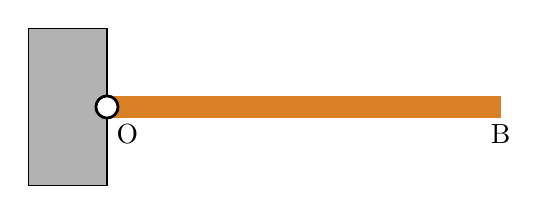
\begin{tikzpicture}
			\coordinate (O) at (0,0);
			\draw[fill=gray!60!white] (0,1) rectangle (-1,-1);
			\draw[line width=8pt, orange!40!brown] (0,0)--(5,0);
			\draw[line width=1pt, fill=white] (0,0) circle(4pt);
			\node[below right] at (0,-0.1) {O};
			\node[below] at (5,-0.1) {B};
		\end{tikzpicture}
	\end{center}
	\choice
	{$\SI{15}{\newton}$}
	{\True $\SI{25}{\newton}$}
	{$\SI{10}{\newton}$}
	{$\SI{30}{\newton}$}
	\loigiai{}
\end{ex}
% ===================================================================
\begin{ex}\mkstar{3}
	Một thanh đồng chất có chiều dài $L$, trọng lượng $\SI{200}{\newton}$, treo một vật có trọng lượng $\SI{450}{\newton}$ vào thanh như hình \ref{fig:23.5}. Các lực $\vec F_1$, $\vec F_2$ của thanh tác dụng lên hai điểm tựa có độ lớn lần lượt là
	\begin{center}
		\includegraphics[width=0.4\linewidth]{../figs/VN10-2022-PH-TP023-P-5}
		\captionof{figure}{}
		\label{fig:23.5}
	\end{center}
	\choice
	{\True $\SI{212.5}{\newton}$; $\SI{437.5}{\newton}$}
	{$\SI{325}{\newton}$; $\SI{325}{\newton}$}
	{$\SI{437.5}{\newton}$; $\SI{212.5}{\newton}$}
	{$\SI{487.5}{\newton}$; $\SI{162.5}{\newton}$}
	\loigiai{Các lực thành phần theo phương $Oy$ cân bằng nhau:
		\begin{equation}
			\label{eq:23.1}
			F_1+F_2-200-450=0
		\end{equation}
		Áp dụng quy tắc moment lực đối với trục quay tại A:
		\begin{equation}
			\label{eq:23.2}
			\dfrac{L}{2}\cdot 200+\dfrac{3L}{4}\cdot 450=LF_2
		\end{equation}
		Từ (\ref{eq:23.1}) và (\ref{eq:23.2}), suy ra $F_1=\SI{212.5}{\newton}$, $F_2=\SI{437.5}{\newton}$.}
\end{ex}
% ===================================================================
\begin{ex}\mkstar{3}
Một đường ống đồng chất có trọng lượng $\SI{100}{\newton}$, chiều dài $L$, tựa trên điểm tựa như hình \ref{fig:23.3}. Khoảng cách $x$ và độ lớn phản lực $F_R$ của điểm tựa tác dụng lên đường ống là
\begin{center}
	\includegraphics[width=0.4\linewidth]{../figs/VN10-2022-PH-TP023-P-3}
	\captionof{figure}{}
	\label{fig:23.3}
\end{center}	
	\choice
	{\True $x=0,69L$; $F_R=\SI{800}{\newton}$}
	{$x=0,69L$; $F_R=\SI{400}{\newton}$}
	{$x=0,6L$; $F_R=\SI{552}{\newton}$}
	{$x=0,6L$; $F_R=\SI{248}{\newton}$}
	\loigiai{Áp dụng quy tắc moment lực đối với trục quay tại A:
		\begin{center}
			\includegraphics[width=0.4\linewidth]{../figs/VN10-2022-PH-TP023-P-4}
		\end{center}
		$$x\cdot 200+\left(x-\dfrac{L}{2}\right)\cdot100=\left(L-x\right)\cdot500$$
		$$\Rightarrow x=0,69L$$
		Các lực thành phần theo phương $Oy$:
		$$F_R-200-100-500=0\Rightarrow F_R=\SI{800}{\newton}.$$}
\end{ex}
% ===================================================================
\begin{ex}\mkstar{3}
	Một thanh chắn đường dài $\SI{7.8}{\meter}$, có trọng lượng $\SI{2100}{\newton}$ và có trọng tâm
	ở cách đầu bên trái $\SI{1.2}{\meter}$. Thanh có thể quay quanh một trục nằm ngang ở cách đầu bên trái $\SI{1.5}{\meter}$. Hỏi phải tác dụng vào đầu bên phải một lực có độ lớn tối thiểu bằng bao nhiêu để thanh ấy nằm ngang?
	\choice
	{\True $\SI{100}{\newton}$}
	{$\SI{200}{\newton}$}
	{$\SI{300}{\newton}$}
	{$\SI{400}{\newton}$}
	\loigiai{\begin{center}
			\includegraphics[width=0.4\linewidth]{../figs/VN10-2022-PH-TP023-P-1}
		\end{center}
		Áp dụng quy tắc moment cho trục quay qua O:
		$$P\cdot OG=F\cdot OB$$
		$$\Rightarrow F=\dfrac{P\cdot OG}{OB}=\dfrac{\left(\SI{2100}{\newton}\right)\cdot\left(\SI{0.3}{\meter}\right)}{\SI{7.8}{\meter}-\SI{1.5}{\meter}}=\SI{100}{\newton}.$$}
\end{ex}
% ===================================================================
\begin{ex}\mkstar{3}
Một tấm ván nặng $\SI{270}{\newton}$ được bắc qua một con mương. Trọng tâm của tấm ván cách điểm tựa trái $\SI{0.8}{\meter}$ và cách điểm tựa phải là $\SI{1.6}{\meter}$. Hỏi lực mà tấm ván tác dụng lên điểm tựa bên trái có độ lớn là bao nhiêu?	
	\choice
	{\True $\SI{180}{\newton}$}
	{$\SI{90}{\newton}$}
	{$\SI{160}{\newton}$}
	{$\SI{80}{\newton}$}
	\loigiai{\begin{center}
			\includegraphics[width=0.4\linewidth]{../figs/VN10-2022-PH-TP023-P-2}
		\end{center}
		Áp dụng quy tắc moment cho trục quay qua điểm tựa phải:
		$$P\cdot d_2=F'_1\cdot\left(d_1+d_2\right)$$
		với $\vec F'_1=-\vec F_1$ là lực do điểm tựa trái tác dụng lên ván.
		$$\Rightarrow F'_1=\dfrac{P\cdot d_2}{d_1+d_2}=\SI{180}{\newton}$$
		Lực do ván tác dụng lên điểm tựa trái:
		$$F_1=F'_1=\SI{180}{\newton}.$$}
\end{ex}
% ===================================================================
\begin{ex}\mkstar{3}
	Một thanh nhẹ gắn vào sàn tại B như hình vẽ.
	\begin{center}
		\includegraphics[scale=1]{../figs/VN10-2021-PH-TP021-6.png}
	\end{center}
	Tác dụng lên đầu A lực kéo $F=\SI{100}{N}$ theo phương ngang. Thanh được giữ cân bằng nhờ dây AC. Lực căng của dây có giá trị là bao nhiêu? Biết $\alpha = \SI{30}{\degree}$.
	\choice
	{$\SI{250}{N}$}
	{$\SI{150}{N}$}
	{$\SI{100}{N}$}
	{\True $\SI{200}{N}$}
	\loigiai{Chọn trục quay tại B. Áp dụng quy tắc moment lực:
		$$F \cdot \text{AB} = T \cdot \text{AB} \cdot \sin \alpha \Rightarrow T = \dfrac{F}{\sin \alpha} = \SI{200}{N}$$}
\end{ex}
% ===================================================================
\begin{ex}\mkstar{4}
	Bán cầu đồng chất khối lượng $\SI{100}{g}$. Trên mép bán cầu đặt một vật nhỏ khối lượng $\SI{7.5}{g}$. Hỏi mặt phẳng của bán cầu sẽ nghiêng góc $\alpha$ bao nhiêu khi nó cân bằng? Biết rằng trọng tâm bán cầu cách mặt phẳng của bán cầu một đoạn $3R/8$ (với $R$ là bán kính của bán cầu).
	\begin{center}
		\includegraphics[scale=1]{../figs/VN10-2021-PH-TP021-7.png}
	\end{center}
	\choice
	{\True $11,31^\circ$}
	{$15^\circ$}
	{$20^\circ$}
	{$12^\circ$}
	\loigiai{	\begin{center}
			\includegraphics[scale=1]{../figs/VN10-2021-PH-TP021-8.png}
		\end{center}
		
		Các lực tác dụng lên bán cầu: trọng lực $\vec P$ của bán cầu, trọng lực $\vec p$ của vật nhỏ, phản lực $\vec Q$ tại điểm tiếp xúc A.
		
		Áp dụng quy tắc moment lực với trục quay qua O:
		$$P \cdot \text{OG} \cdot \sin \alpha = p \cdot R \cdot \cos \alpha \Rightarrow \tan \alpha = \dfrac{8m}{3M} \Rightarrow \alpha = 11,31^\circ$$}
\end{ex}
% ===================================================================
\begin{ex}\mkstar{4}
	Một cái thang có cấu tạo đồng đều được đặt dựa vào tường trơn nhẵn. 
	\begin{center}
		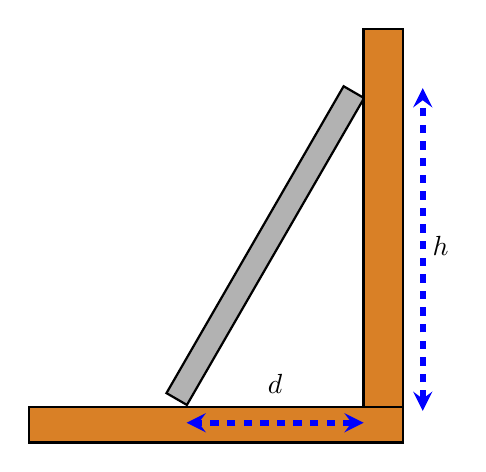
\begin{tikzpicture}
			\coordinate (O) at (0,0);
			\draw[stealth-stealth, line width=2pt, blue, dashed] (2,-2.1)--(2,2);
			
			\node [draw, thick, shape=rectangle, minimum width=0.3cm, minimum height=4.5cm, anchor=center, fill=gray!60!white, rotate=-30] at (O) {};
			\draw[line width=1pt, fill=orange!40!brown] (1.25,2.75) rectangle (1.75,-2.1);
			\draw[line width=1pt, fill=orange!40!brown] (1.75,-2.05) rectangle (-3,-2.5);
			\draw[stealth-stealth, line width=2pt, blue, dashed] (1.25,-2.25)--(-1,-2.25);
			\node[right] at (2,0) {$h$};
			\node[above] at (0.125,-2) {$d$};
		\end{tikzpicture}
	\end{center}
	Để thang không bị trượt thì hệ số ma sát tĩnh ở chỗ mặt tiếp xúc của thang với sàn nhà phải thỏa điều kiện
	\choice
	{$\mu\le\dfrac{d}{2h}$}
	{\True $\mu\ge\dfrac{d}{2h}$}
	{$\mu\le\dfrac{2h}{d}$}
	{$\mu\le\dfrac{2h}{d}$}
	\loigiai{
	\begin{center}
		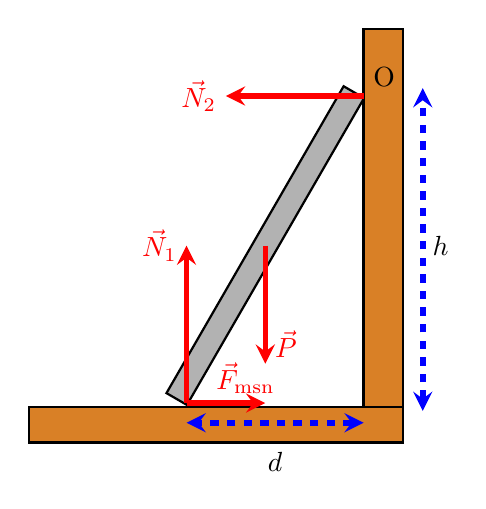
\begin{tikzpicture}
			\coordinate (O) at (0,0);
			\draw[stealth-stealth, line width=2pt, blue, dashed] (2,-2.1)--(2,2);
			
			\node [draw, thick, shape=rectangle, minimum width=0.3cm, minimum height=4.5cm, anchor=center, fill=gray!60!white, rotate=-30] at (O) {};
			\draw[line width=1pt, fill=orange!40!brown] (1.25,2.75) rectangle (1.75,-2.1);
			\draw[line width=1pt, fill=orange!40!brown] (1.75,-2.05) rectangle (-3,-2.5);
			\draw[stealth-stealth, line width=2pt, blue, dashed] (1.25,-2.25)--(-1,-2.25);
			\node[right] at (2,0) {$h$};
			\node[below] at (0.125,-2.5) {$d$};
			\draw[red, line width=2pt, -stealth] (O)--($(O)-(0,1.5)$);
			\draw[red, line width=2pt, -stealth] (-1,-2)--(-1,0);
			\draw[red, line width=2pt, -stealth] (1.25,1.9)--(-0.5,1.9);
			\draw[red, line width=2pt, -stealth] (-1,-2)--(0,-2);
			\node[above,red] at (-0.25,-2) {$\vec{F}_{\text{msn}}$};
			\node[right,red] at (0,-1.25) {$\vec{P}$};
			\node[left,red]  at (-1,0) {$\vec{N}_1$};
			\node[left,red]  at (-0.5,1.9) {$\vec{N}_2$};
			\node[above right] at (1.25,1.9) {O};
		\end{tikzpicture}
	\end{center}
	Áp dụng quy tắc moment cho trục quay qua O:
	$$N_1d=F_{\text{msn}}h+P\cdot\dfrac{d}{2}$$
	Mà $N_1=P$ nên:
	$$F_{\text{msn}}h=P\cdot\dfrac{d}{2}\Rightarrow F_{\text{msn}}=P\cdot\dfrac{d}{2h}.$$
	Lại có:
	$$F_{\text{msn}}\le\mu N_1=\mu P\Rightarrow\mu \ge\dfrac{d}{2h}.$$
	}
\end{ex}
% ===================================================================
\begin{ex}\mkstar{4}
	Một thanh AB đồng chất, tiết diện đều có khối lượng $\SI{3}{\kilogram}$, dài $\SI{2}{\meter}$, có một đầu được gắn bởi một bản lề nhẵn vào trần nhà tại A. Đầu B được buộc vào một sợi dây nhẹ không đàn hồi. Đầu kia của sợi dây được gắn vào trần nhà ở điểm C. Thanh tạo một góc $\SI{30}{\degree}$ với phương ngang và sợi dây tạo một góc $\SI{60}{\degree}$ so với phương ngang như hình bên. 
	\begin{center}
		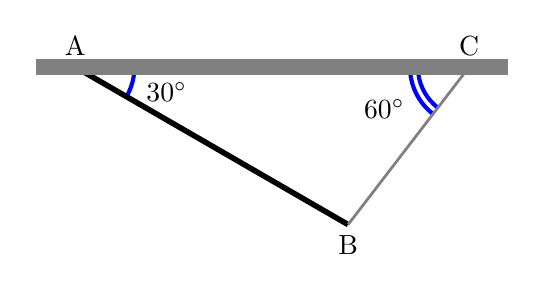
\begin{tikzpicture}
			\coordinate (A) at (0,0);
			\coordinate (B) at ($(A)+(-30:4)$);
			\coordinate (C) at (5,0);
			\tkzMarkAngle[size=0.75cm,color=blue,line width=1.5pt](B,A,C);
			\tkzLabelAngle[color=black,pos=1.2](B,A,C){$\SI{30}{\degree}$};
			\tkzMarkAngle[size=0.75cm,color=blue,line width=1.5pt](A,C,B);
			\tkzMarkAngle[size=0.65cm,color=blue,line width=1.5pt](A,C,B);
			\tkzLabelAngle[color=black,pos=1.2](A,C,B){$\SI{60}{\degree}$};
			\draw[line width=2pt] (A)--(B);
			\draw[line width=1pt, gray] (C)--(B);
			\draw[line width=6pt, gray] (-0.5,0)--(5.5,0);
			\node[above] at (A) {A};
			\node[above] at (C) {C};
			\node[below] at (B) {B};
		\end{tikzpicture}
	\end{center}
	Lấy $g=\SI{10}{\meter/\second^2}$. Lực căng của sợi dây có độ lớn là
	\choice
	{$\SI{7.5}{\newton}$}
	{$\SI{14}{\newton}$}
	{\True $\SI{13}{\newton}$}
	{$\SI{6.5}{\newton}$}
	\loigiai{}
\end{ex}
\Closesolutionfile{ans}
\section{Trắc nghiệm đúng/sai}
\setcounter{ex}{0}
\Opensolutionfile{ans}[ans/VN10-Y24-PH-SYL-023P-TF]
% ===================================================================
\begin{ex}\mkstar{1}
	Xét tính đúng/sai của các phát biểu sau đây khi nói về ngẫu lực.
	\choiceTF[t]
	{Ngẫu lực tác dụng vào một vật sẽ làm vật vừa quay vừa tịnh tiến}
	{Moment của ngẫu lực không chỉ phụ thuộc cánh tay đòn của ngẫu lực mà còn phụ thuộc khoảng cách từ lực đến trục quay}
	{Moment của ngẫu lực phụ thuộc điểm đặt mỗi lực hay vị trí trục quay}
	{\True Ngẫu lực không gây tác dụng lên trục quay}
	\loigiai{\begin{itemchoice}
			\itemch Sai. Ngẫu lực tác dụng vào một vật chỉ làm vật quay.
			\itemch Sai. Moment của ngẫu lực chỉ phụ thuộc cánh tay đòn của ngẫu lực.
			\itemch Sai. Moment của ngẫu lực không phụ thuộc điểm đặt mỗi lực hay vị trí trục quay.
			\itemch Đúng. Ngẫu lực không gây tác dụng lên trục quay.
	\end{itemchoice}}
\end{ex}
% ===================================================================
\begin{ex}\mkstar{2}
	Hai anh em Bình và An đang chơi trò bập bênh. Bập bênh là một tấm ván AB cứng, đồng chất, tiết diện đều và giá đỡ nằm ngay trọng tâm O của tấm ván. AB chia thành 6 đoạn bằng nhau (như hình). Khối lượng của An bằng $\SI{25}{\kilogram}$ còn khối lượng của Bình bằng $\SI{75}{\kilogram}$. An ngồi bên phần OA và Bình ngồi bên phần OB.
	\begin{center}
		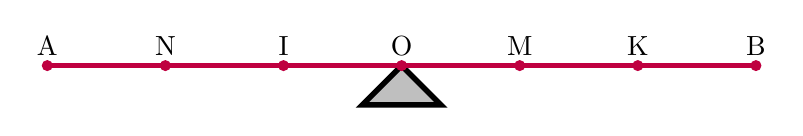
\begin{tikzpicture}
			\draw[line width=2pt, fill=gray!50!white] (0,0)--(-0.5,-0.5)--(0.5,-0.5)--(0,0);
			\draw[line width=2pt, purple] (-4.5,0)--(4.5,0);
			\foreach \i in {-4.5,-3,...,4.5}{
				\fill[fill=purple]   (\i,0) circle[radius=2pt];
			
			};
			\node[above] at (-4.5,0) {A};
			\node[above] at (-1.5,0) {I};
			\node[above] at (-3,0) {N};
			\node[above] at (0,0) {O};
			\node[above] at (1.5,0) {M};
			\node[above] at (3,0) {K};
			\node[above] at (4.5,0) {B};
		\end{tikzpicture}
	\end{center}
	\choiceTF[t]
	{\True Bập bênh trên không có moment trọng lực}
	{Khi Bình và An cùng ngồi tại hai đầu tấm ván thì moment trọng lực của hai anh em bằng nhau }
	{Khi Bình và An cùng ngồi tại hai đầu tấm ván thì bập bênh có xu hướng quay ngược chiều kim đồng hồ}
	{\True Khi An ngồi ở A, để bập bênh ở trạng thái cân bằng nằm ngang thì Bình phải dịch chuyển tới vị trí M}
	\loigiai{
	\begin{itemchoice}
		\itemch Đúng.
		\itemch Sai. Do $\mathrm{OA}=\mathrm{OB}$ và $m_{\text{Bình}}>m_{\text{An}}$ nên $M_{\vec{P}\text{An}}<M_{\vec{P}{\text{Bình}}}$.
		\itemch Sai. Do $M_{\vec{P}\text{An}}<M_{\vec{P}\text{Bình}}$ nên bập bênh có xu hướng quay cùng chiều kim đồng hồ.
		\itemch Đúng.
	\end{itemchoice}
	}
\end{ex}
% ===================================================================
\begin{ex}\mkstar{3}
	Một thanh ngang AB có khối lượng $\SI{4}{\kilogram}$ như hình bên. Đầu A của thanh treo một thùng hàng có khối lượng $\SI{50}{\kilogram}$. Thanh AB dài $\SI{3}{\meter}$ và có vạch chia đều. Lấy $g=\SI{10}{\meter/\second^2}$.
	\begin{center}
		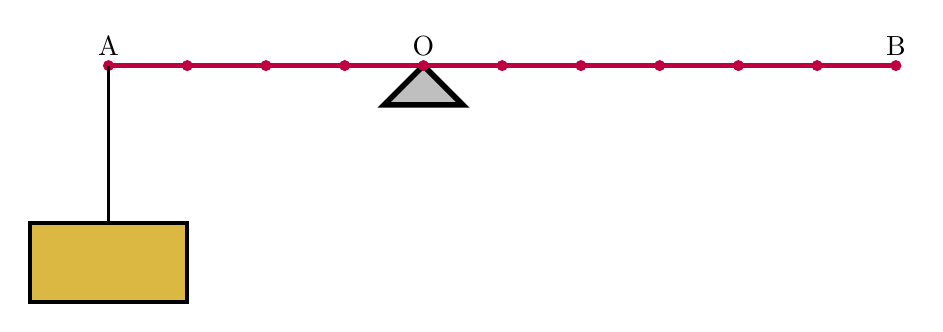
\begin{tikzpicture}
			\draw[line width=2pt, fill=gray!50!white] (0,0)--(-0.5,-0.5)--(0.5,-0.5)--(0,0);
			\draw[line width=2pt, purple] (-4,0)--(6,0);
			\foreach \i in {-4,-3,...,6}{
				\fill[fill=purple]   (\i,0) circle[radius=2pt];
				
			};
			\draw[line width=1pt] (-4,0)--(-4,-2);
			\draw[line width=1.5pt, fill=yellow!40!brown] (-5,-2) rectangle (-3,-3);
			\node[above] at(-4,0) {A};
			\node[above] at(0,0) {O};
			\node[above] at(6,0) {B};
		\end{tikzpicture}
	\end{center}
	\choiceTF[t]
	{Cánh tay đòn của moment trọng lực thùng hàng đối với trục quay O là $\SI{1.5}{\meter}$}
	{Thanh AB không có moment đối với trục quay tại O}
	{\True Moment của trọng lực thùng hàng đối với trục quay tại O bằng $\SI{600}{\newton\meter}$}
	{\True Để thanh cân bằng cần treo vào điểm chính giữa của OB một vật có khối lượng $m'=\xsi{\dfrac{196}{3}}{\kilogram}$}
	\loigiai{
	\begin{itemchoice}
		\itemch Sai. Cánh tay đòn của moment trọng lực thùng hàng đối với trục quay O là $\mathrm{OA}=\SI{1.2}{\meter}$.
		\itemch Sai. Thanh AB có $P=mg=\SI{40}{\newton}$ và điểm đặt của trọng lực tại I cách trục quay O đoạn $\mathrm{OI}=\SI{0.3}{\meter}$ nên có moment.
		\itemch Đúng.
		\itemch Đúng.
	\end{itemchoice}
	}
\end{ex}
\Closesolutionfile{ans}
\section{Tự luận}
\setcounter{ex}{0}
\Opensolutionfile{ans}[ans/VN10-Y24-PH-SYL-023P-TL]
\begin{ex}\mkstar{2}
	Biết các lực $F_1=\SI{25}{\newton}$, $F_2=\SI{10}{\newton}$, $F_3=\SI{10}{\newton}$ tác dụng vào thanh AB có trục quay tại A như hình vẽ.
	\begin{center}
		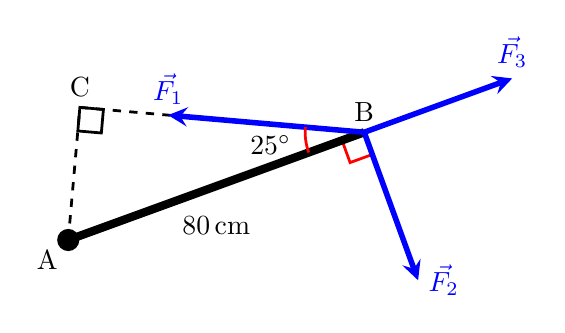
\begin{tikzpicture}
			\coordinate (B) at (0,0);
			\coordinate (A)  at ($(B)+(200:4)$);
			\coordinate (F1)  at ($(B)+(175:2.5)$);
			\coordinate (F3)  at ($(B)+(20:2)$);
			\coordinate (F2)  at ($(B)+(-70:2)$);
			\coordinate (C)  at ($(B)+(175:3.625)$);
			\tkzMarkRightAngle[size=0.3,color=red, line width=1pt](A,B,F2);
			\tkzMarkRightAngle[size=0.3, line width=1pt](A,C,B);
			\draw[line width=3pt] (A)--(B);
			\draw[dashed, line width=1pt] (A)--(C)--(B);
			\draw[blue, line width=2pt, -stealth] (B)--(F1);
			\draw[blue, line width=2pt, -stealth] (B)--(F2);
			\draw[blue, line width=2pt, -stealth] (B)--(F3);
			\fill   (A) circle[radius=4pt]  node [below left] {A};
			\node[above, blue] at (F1) {$\vec{F_1}$};
			\node[above, blue] at (F3) {$\vec{F_3}$};
			\node[right, blue] at (F2) {$\vec{F_2}$};
			\node[above] at (B) {B};
			\node[above] at (C) {C};
			\node[below] at ($(A)!0.5!(B)-(0,0.25)$) {$\SI{80}{\centi\meter}$};
				\tkzMarkAngle[size=0.75cm,color=red, line width=1pt](F1,B,A);
			\tkzLabelAngle[color=black,pos=1.2](F1,B,A){$\SI{25}{\degree}$};
			
		\end{tikzpicture}
	\end{center}
	\begin{enumerate}[label=\alph*)]
		\item Các lực $\vec{F}_1$; $\vec{F}_2$; $\vec{F}_3$ tác dụng lên thanh làm cho thanh quay theo chiều nào?
		\item Xác định cánh tay đòn của các lực $\vec{F}_1$; $\vec{F}_2$ và $\vec{F}_3$ đối với trục quay qua A.
		\item Tính độ lớn moment của các lực $\vec{F}_1$; $\vec{F}_2$; $\vec{F}_3$ đối với trục quay qua A.
	\end{enumerate}
	\loigiai{
	\begin{enumerate}[label=\alph*)]
		\item Lực $\vec{F}_1$ làm cho thanh quay ngược chiều kim đồng hồ.\\
		Lực $\vec{F}_2$ làm cho thanh quay cùng chiều kim đồng hồ.
		\\
		Lực $\vec{F}_3$ không có tác dụng làm cho thanh quay vì giá của lực đi qua trục quay.
		\item Cánh tay đòn của các lực:\\
		$d_1=\mathrm{AC}=\mathrm{AB}\sin\SI{25}{\degree}=\SI{0.338}{\meter}$\\
		$d_2=\mathrm{AB}=\SI{0.8}{\meter}$\\
		$d_3=0$.
		\item Moment của lực đối với trục quay qua A:\\
		$M_{F_1}=F_1d_1=\left(\SI{25}{\newton}\right)\cdot\left(\SI{0.8}{\meter}\right)\cdot\sin\SI{25}{\degree}=\SI{8.45}{\newton\meter}$.\\
		$M_{F_2}=F_2\cdot d_2=\left(\SI{10}{\newton}\right)\cdot\left(\SI{0.8}{\meter}\right)=\SI{8}{\newton\meter}$.
		\\
		$M_{F_3}=F_3d_3=0$.
	\end{enumerate}
	}
\end{ex}
% ======================================================================
\begin{ex}\mkstar{2}
	Một chiếc thước mảnh có trục quay nằm ngang đi qua trọng tâm O của thước. Dùng hai ngón tay tác dụng vào thước một ngẫu lực đặt vào hai điểm A và B cách nhau $\SI{4.5}{\centi\meter}$ và có độ lớn $F_{\mathrm{A}}=F_{\mathrm{B}}=\SI{1}{\newton}$.
	Thước quay đi một góc $\alpha=\SI{30}{\degree}$. Hai lực luôn luôn nằm ngang và vẫn đặt tại A và B (hình vẽ).
	\begin{center}
		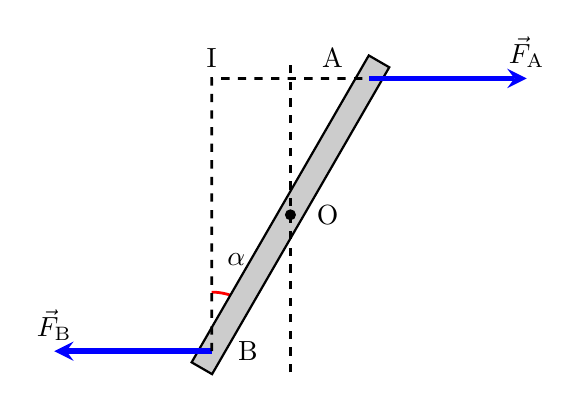
\begin{tikzpicture}
			\coordinate (O) at (0,0);
			\coordinate (A) at ($(O)+(60:2)$);
			\coordinate (B) at ($(O)+(-120:2)$);
			\coordinate (FA) at ($(A)+(2,0)$);
			\coordinate (FB) at ($(B)+(-2,0)$);
			\coordinate (I) at ($(B)+(90:3.4641)$);
			\tkzMarkAngle[size=0.75cm,color=red, line width=1pt](A,B,I);
			\node [draw, thick, shape=rectangle, minimum width=0.3cm, minimum height=4.5cm, anchor=center, fill=gray!40!white, rotate=-30] at (O) {};
			\fill   (O) circle[radius=2pt]  node [right] {};
			\draw[line width=2pt, -stealth, line width=2pt, blue] (A)--(FA);
			\draw[line width=2pt, -stealth, line width=2pt, blue] (B)--(FB);
			\draw[dashed, line width=1pt] (B)--(I)--(A);
			\draw[dashed, line width=1pt] (0,-2)--(0,2);
			\node[right] at ($(B)+(0.2,0)$) {B};
			\node[above left] at ($(A)+(-0.2,0)$) {A};
			\node[right] at ($(O)+(0.2,0)$) {O};
			\node[above] at (I) {I};
			\node[above] at (FA) {$\vec{F}_{\mathrm{A}}$};
			\node[above] at (FB) {$\vec{F}_{\mathrm{B}}$};
			
			\tkzLabelAngle[color=black,pos=1.2](A,B,I){$\alpha$};
		\end{tikzpicture}
	\end{center}
	\loigiai{}
\end{ex}
% ======================================================================
\begin{ex}\mkstar{2}
	Thanh AB khối lượng $m$, chiều dài $L=\SI{3}{\meter}$ gắn vào tường với bản lề A. Đầu B của thanh treo vật nặng $\SI{5}{\kilogram}$. Thanh được giữ nằm ngang nhờ dây treo CD, biết lực căng dây $\SI{150}{\newton}$, $\mathrm{AC}=\SI{2}{\meter}$, dây treo hợp với thanh AB một góc $\alpha=\SI{45}{\degree}$ như hình vẽ bên dưới. 
	\begin{center}
		\includegraphics[width=0.25\linewidth]{../figs/VN10-2022-PH-TP023-P-11}
	\end{center}
	Xác định moment của lực căng dây CD và moment lực căng dây ở đầu B đối với trục quay qua A. Lấy $g=\SI{10}{\meter/\second^2}$.	
	\loigiai{
	Moment của lực căng dây:
	$M_{T_{\mathrm{B}/\mathrm{A}}}=T_{\mathrm{B}}\cdot\mathrm{AB}=m_{\mathrm{B}}g\cdot\mathrm{AB}=\SI{150}{\newton\meter}$.
	\\
	$M_{T_{\mathrm{CD}/\mathrm{A}}}=T_{\mathrm{CD}}\cdot\mathrm{AC}\sin\alpha=\xsi{150\sqrt{2}}{\newton\meter}$.
		}
\end{ex}
% ======================================================================
\begin{ex}\mkstar{2}
	Một cái thước $AB=\SI{1.2}{\meter}$ đặt trên mặt bàn nhẵn nằm ngang, có trục quay O cách đầu A một khoảng $\SI{80}{\centi\meter}$. Một lực $F_1=\SI{5}{\newton}$ tác dụng lên đầu A theo phương vuông góc với thước và lực thứ hai tác dụng lên đầu B của thước theo phương vuông góc với thước. Các lực đều nằm trên mặt phẳng nằm ngang. Nếu thước không chuyển động thì lực tác dụng vào đầu B của thước có hướng và độ lớn như thế nào?
		\begin{center}
		\includegraphics[width=0.35\linewidth]{../figs/VN10-2022-PH-TP023-P-8}
	\end{center}
	\loigiai{$\vec F_2$ cùng hướng với $\vec F_1$.\\
		Áp dụng quy tắc moment cho trục quay qua O:
		$$F_1\cdot OA=F_2\cdot OB\Rightarrow F_2=\dfrac{F_1\cdot OA}{OB}=\dfrac{\left(\SI{5}{\newton}\right)\cdot\left(\SI{0.8}{\meter}\right)}{\SI{0.4}{\meter}}=\SI{10}{\newton}.$$}
\end{ex}
% ======================================================================
\begin{ex}\mkstar{2}
	Một thanh kim loại đồng chất AB dài $\SI{2}{\meter}$ có tiết diện đều và khối lượng của thanh là $\SI{2}{\kilo\gram}$. Người ta treo vào đầu A của thanh một vật có khối lượng $\SI{5}{\kilogram}$, đầu B một vật có khối lượng $\SI{1}{\kilogram}$. Hỏi phải đặt một giá đỡ tại điểm O cách đầu A một khoảng là bao nhiêu để thanh cân bằng?
	\loigiai{\begin{center}
			\includegraphics[width=0.3\linewidth]{../figs/VN10-2022-PH-TP023-P-9}
		\end{center}
		Gọi O là vị trí điểm tựa.\\
		Áp dụng quy tắc moment cho trục quay qua O:
		\begin{eqnarray*}
			&&P_\text{A}\cdot OA=P\cdot OG+P_\text{B}\cdot OB\\
			&\Leftrightarrow &P_\text{A}\cdot OA=P\cdot\left(\dfrac{AB}{2}-OA\right)+P_\text{B}\cdot\left(AB-OA\right)\\
			&\Leftrightarrow &50\cdot OA=20\cdot\left(1-OA\right)+10\cdot\left(2-OA\right)\\
			&\Rightarrow &OA=\SI{0.5}{\meter}.
	\end{eqnarray*}}
\end{ex}

% ======================================================================
\begin{ex}\mkstar{3}
	Một thanh sắt dài, đồng chất, tiết diện đều, được đặt trên bàn sao cho $\frac{1}{4}$ chiều dài của nó nhô ra khỏi bàn. Tại đầu nhô ra, người ta đặt một lực $\vec F$ thẳng đứng hướng xuống dưới. Khi lực đạt tới giá trị $\SI{40}{\newton}$ thì đầu kia của thanh sắt bắt đầu bênh lên. Hỏi trọng lượng của thanh sắt bằng bao nhiêu?
	\begin{center}
		\includegraphics[width=0.4\linewidth]{../figs/VN10-2022-PH-TP023-P-10}
	\end{center}
	\loigiai{Áp dụng quy tắc moment với điểm tựa tại cạnh bàn:
		\begin{eqnarray*}
			&&P\cdot\left(\dfrac{L}{2}-\dfrac{L}{4}\right)=F\cdot\dfrac{L}{4}\\
			&\Rightarrow& F=P=\SI{40}{\newton}.
	\end{eqnarray*}}
\end{ex}
% ======================================================================
\begin{ex}\mkstar{3}
Một thanh có độ dài $L$, trọng lượng $\SI{10}{\newton}$, được treo nằm ngang vào tường như hình \ref{fig:23.6}. Một vật có trọng lượng $\SI{20}{\newton}$ treo ở đầu thanh. Dây treo hợp với thanh một góc $\alpha=\SI{30}{\degree}$. Xác định độ lớn lực căng dây treo.
\begin{center}
	\includegraphics[width=0.4\linewidth]{../figs/VN10-2022-PH-TP023-P-6}
	\captionof{figure}{}
	\label{fig:23.6}
\end{center}	
	\loigiai{Áp dụng quy tắc moment đối với trục quay qua O:
		\begin{center}
			\includegraphics[width=0.35\linewidth]{../figs/VN10-2022-PH-TP023-P-7}
		\end{center}
		$$0\cdot N+OH\cdot T=\dfrac{L}{2}\cdot P+L\cdot P_1$$
		$$\Leftrightarrow T\cdot L\sin\alpha=\dfrac{L}{2}\cdot P+L\cdot P_1$$
		$$\Rightarrow T=\dfrac{\dfrac{P}{2}+P_1}{\sin\alpha}=\dfrac{\SI{5}{\newton}+\SI{20}{\newton}}{\sin\SI{30}{\degree}}=\SI{50}{\newton}.$$}
\end{ex}
% ======================================================================
\begin{ex}\mkstar{3}
	Dùng cân đòn để cân một vật. Vì cánh tay đòn của cân không thật bằng nhau nên khi đặt vật ở đĩa cân bên này thì người ta cân được $\SI{40}{\gram}$ nhưng khi đặt vật sang đĩa cân bên kia, người ta cân được $\SI{44.1}{\gram}$. Lấy $g=\SI{10}{\meter/\second^2}$.
	 Tìm khối lượng đúng của vật.
	\begin{center}
		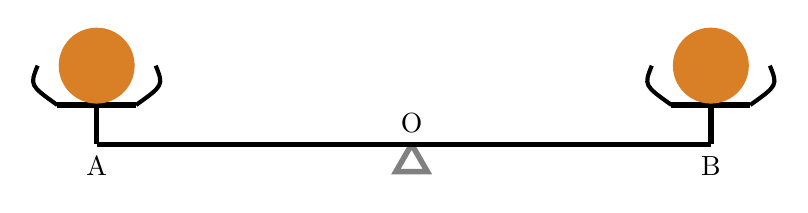
\begin{tikzpicture}
			\coordinate (A) at (-4,0);
			\coordinate (B) at (3.8,0);
			\coordinate (O) at (0,0);
			\draw[line width=2pt, gray] (O)--($(O)+(-60:0.4)$)--($(O)+(-120:0.4)$)--(O);
			\draw[line width=2pt] (A) node [below]{A}--(O) node [above]{O}--(B) node[below] {B};
			\draw[line width=2pt] (A)--($(A)+(0,0.5)$);
			\draw[line width=2pt] (-4.5,0.5)--(-3.5,0.5);
			\draw[line width=1.5pt] (-4.5,0.5) ..controls (-4.85,0.75)..(-4.75,1);
			\draw[line width=1.5pt] (-3.5,0.5) ..controls (-3.15,0.75)..(-3.25,1);
			\draw[line width=2pt] (3.3,0.5)--(4.3,0.5);
			\draw[line width=1.5pt] (3.3,0.5) ..controls (2.95,0.75)..(3.05,1);
			\draw[line width=1.5pt] (4.3,0.5) ..controls (4.65,0.75)..(4.55,1);
			\draw[line width=2pt] (B)--($(B)+(0,0.5)$);
			\filldraw[orange!40!brown] (-4,1) circle (0.475);
			\filldraw[orange!40!brown] (3.8,1) circle (0.475);
		\end{tikzpicture}
	\end{center}
	\loigiai{
	Gọi $m$ là khối lượng vật.\\
	Áp dụng quy tắc moment cho trục quay qua O:
	$$\begin{cases}
		P\cdot\mathrm{OA}=P_1\cdot\mathrm{OB}\\
		P_2\cdot\mathrm{OA}=P\cdot\mathrm{OB}
	\end{cases}\Rightarrow \dfrac{P}{P_2}=\dfrac{P_1}{P}.$$
	Như vậy:
	$$m=\sqrt{m_1m_2}=\SI{42}{\gram}.$$
	}
\end{ex}
% ======================================================================
\begin{ex}\mkstar{4}
	Một vật rắn phẳng, mỏng, có dạng là một hình vuông ABCD, mỗi cạnh là $a=\SI{10}{cm}$. Người ta tác dụng một ngẫu lực nằm trong mặt phẳng của hình vuông. Biết các lực vuông góc với đường chéo AD có độ lớn $\SI{10}{N}$ và đặt vào hai đỉnh của A và D. Tính moment của ngẫu lực.
	\loigiai{Ta có đường chéo của hình vuông:
		$$d=\sqrt{a^2 + a^2} = \SI{14.14}{cm} = \SI{0.14}{m}$$
		
		Moment ngẫu lực:
		$$M=Fd = \SI{1.41}{Nm}$$}
\end{ex}
\Closesolutionfile{ans}

				\stopMyChapterToc
		\stopPartToc
	\chapter*{Ôn tập chương \thepart}
		\addcontentsline{toc}{mychapter}{\bfseries Ôn tập chương \thepart}
		\let\lesson\undefined
\newcommand{\lesson}{\phantomlesson{Ôn tập chương 5}}
\setcounter{ex}{0}
\hideall{
\inputansbox{10}{ans/VN10-2023-PH-TP0005-TN}
}
\setcounter{section}{2}
\setcounter{ex}{0}
\Opensolutionfile{ans}[ans/VN10-2023-PH-TP0005-TN]
% ===================================================================
\begin{ex}
	Đơn vị của moment lực là
	\choice
	{$\si{\meter/\second}$}
	{\True $\si{\newton\cdot\meter}$}
	{$\si{\kilogram\cdot\meter}$}
	{$\si{\newton\cdot\kilogram}$}
	\loigiai{}
\end{ex}
% ===================================================================
\begin{ex}
	Moment lực tác dụng lên vật là đại lượng
	\choice
	{\True đặc trưng cho tác dụng làm quay vật của lực}
	{vô hướng}
	{để xác định độ lớn của lực tác dụng}
	{luôn có giá trị dương}
	\loigiai{}
\end{ex}
% ===================================================================
\begin{ex}
Moment lực tác dụng lên một vật có trục quay cố định là đại lượng	
	\choice
	{đặc trưng cho tác dụng làm quay vật của lực và được đo bằng tích số của lực với khoảng cách từ điểm đặt lực đến trục quay}
	{\True đặc trưng cho tác dụng làm quay vật của lực và được đo bằng tích của lực và cánh tay đòn của nó}
	{đặc trưng cho độ mạnh yếu của lực}
	{luôn có giá trị âm}
	\loigiai{}
\end{ex}
% ===================================================================
\begin{ex}
	Theo quy tắc hợp lực song song cùng chiều. Điểm đặt của hợp lực được xác định dựa trên biểu thức sau
	\choice
	{$\dfrac{F_1}{F_2}=\dfrac{d_1}{d_2}$}
	{\True $\dfrac{F_1}{F_2}=\dfrac{d_2}{d_1}$}
	{$\dfrac{F_2}{F_1}=\dfrac{d_2}{d_2+d_1}$}
	{$\dfrac{F_2}{F_1}=\dfrac{d_1}{d_2+d_1}$}
	\loigiai{}
\end{ex}
% ===================================================================
\begin{ex}
	Phát biểu nào sau đây đúng với quy tắc moment lực?
	\choice
	{\True Muốn cho một vật có trục quay cố định nằm cân bằng thì tổng moment của các lực có khuynh hướng làm vật quay theo một chiều phải bằng tổng moment của các lực có khuynh hướng làm vật quay theo chiều ngược lại}
	{Muốn cho một vật có trục quay cố định nằm cân bằng thì tổng moment của các lực phải bằng hằng số}
	{Muốn cho một vật có trục quay cố định nằm cân bằng thì tổng moment của các lực phải khác không}
	{Muốn cho một vật có trục quay cố định nằm cân bằng thì tổng moment của các lực phải là một vector có giá đi qua trục quay}
	\loigiai{}
\end{ex}
% ===================================================================
\begin{ex}
	Lực có tác dụng làm cho vật rắn quay quanh một trục khi
	\choice
	{lực có giá nằm trong mặt phẳng vuông góc với trục quay và cắt trục quay}
	{lực có giá song song với trục quay}
	{lực có giá cắt trục quay}
	{\True lực có giá nằm trong mặt phẳng vuông góc với trục quay và không cắt trục quay}
	\loigiai{}
\end{ex}
% ===================================================================
\begin{ex}
	Nhận xét nào sau đây về ngẫu lực là \textbf{không chính xác}?
	\choice
	{\True Hợp lực của ngẫu lực tuân theo quy tắc tổng hợp hai lực song song, ngược chiều}
	{Ngẫu lực là hệ gồm hai lực song song, ngược chiều và có độ lớn bằng nhau}
	{Moment của ngẫu lực tính theo công thức $M=F\cdot d$ (trong đó $d$ là cánh tay đòn của ngẫu lực)}
	{Nếu vật không có trục quay cố định chịu tác dụng của ngẫu lực thì nó sẽ quay quanh một trục đi qua trọng tâm và vuông góc với mặt phẳng chứa ngẫu lực}
	\loigiai{Ngẫu lực không có hợp lực vì không thể tìm được 1 lực duy nhất thay thế tác dụng của ngẫu lực}
\end{ex}
% ===================================================================
\begin{ex}
	Điều kiện để một vật nằm cân bằng là
	\choice
	{tổng moment lực tác dụng lên vật phải bằng không}
	{hợp lực tác dụng lên vật phải bằng không}
	{\True hợp lực tác dụng lên vật phải bằng không và tổng moment lực tác dụng lên vật phải bằng không}
	{yrọng lực và phản lực có nó phải cân bằng nhau}
	\loigiai{}
\end{ex}
% ===================================================================
\begin{ex}
	Người làm xiếc đi trên dây thường cầm một cây gậy nặng để làm gì?
	\choice
	{Để vừa đi vừa biểu diễn cho đẹp}
	{Để tăng lực ma sát giữa chân người và dây}
	{\True Để điều chỉnh cho giá trọng lực của người và gậy luôn đi qua dây}
	{Để tăng moment trọng lực của người và gậy}
	\loigiai{}
\end{ex}
% ===================================================================
\begin{ex}
Khi dùng tua vít để vặn đinh vít, người ta đã tác dụng vào các đinh vít	
	\choice
	{\True một ngẫu lực}
	{hai ngẫu lực}
	{cặp lực cân bằng}
	{cặp lực trực đối}
	\loigiai{}
\end{ex}
% ===================================================================
\begin{ex}
Một lực $F$ tác dụng lên vật rắn, khi điểm đặt của lực $F$ dời chỗ trên giá của nó thì tác dụng của lực đó lên vật rắn	
	\choice
	{tăng lên}
	{giảm xuống}
	{\True không đổi}
	{bằng không}
	\loigiai{}
\end{ex}
% ===================================================================
\begin{ex}
	Hai lực của ngẫu lực có độ lớn $F=\SI{20}{\newton}$, khoảng cách giữa hai giá của ngẫu lực là $d=\SI{30}{\centi\meter}$. Moment của ngẫu lực là
	\choice
	{$M=\SI{0.6}{\newton\cdot\meter}$}
	{$M=\SI{600}{\newton\cdot\meter}$}
	{\True $M=\SI{6}{\newton\cdot\meter}$}
	{$M=\SI{60}{\newton\cdot\meter}$}
	\loigiai{Moment ngẫu lực:
		$$M=Fd=\left(\SI{20}{\newton}\right)\cdot\left(\SI{0.3}{\meter}\right)=\SI{6}{\newton\cdot\meter}.$$}
\end{ex}
% ===================================================================
\begin{ex}
	Một vật rắn phẳng, mỏng, dạng tam giác đều ABC, cạnh $a=\SI{20}{\centi\meter}$. Người ta tác dụng vào một ngẫu lực nằm trong mặt phẳng của tam giác. Các lực có độ lớn $\SI{8}{\newton}$ và đặt vào hai đỉnh A và C, song song với BC. Moment của ngẫu lực có độ lớn là
	\choice
	{$\SI{13.8}{\newton\cdot\meter}$}
	{\True $\SI{1.38}{\newton\cdot\meter}$}
	{$\SI{13.8E-2}{\newton\cdot\meter}$}
	{$\SI{13.8E-3}{\newton\cdot\meter}$}
	\loigiai{Cánh tay đòn ngẫu lực chính bằng đường cao kẻ từ A của tam giác ABC:
		$$d=AH=\dfrac{a\sqrt{3}}{2}=\xsi{10\sqrt{3}}{\centi\meter}$$
		Moment của ngẫu lực:
		$$M=Fd=\left(\SI{8}{\newton}\right)\cdot\left(\xsi{0,1\sqrt{3}}{\meter}\right)=\SI{1.38}{\newton\cdot\meter}.$$}
\end{ex}
% ===================================================================
\begin{ex}
	Một lực có độ lớn $\SI{10}{\newton}$ tác dụng lên một vật rắn quay quanh một trục cố định, biết khoảng cách từ giá của lực đến trục quay là $\SI{20}{\centi\meter}$. Moment của lực tác dụng lên vật có giá trị là
	\choice
	{$\SI{200}{\newton\cdot\meter}$}
	{$\SI{200}{\newton/\meter}$}
	{\True $\SI{2}{\newton\cdot\meter}$}
	{$\SI{2}{\newton/\meter}$}
	\loigiai{Moment của lực tác dụng lên vật:
		$$M=Fd=\left(\SI{10}{\newton}\right)\cdot\left(\SI{0.2}{\meter}\right)=\SI{2}{\newton\cdot\meter}.$$}
\end{ex}
% ===================================================================
\begin{ex}
Một người gánh một thúng lúa và một thúng gạo, thúng lúa nặng $\SI{10}{\kilogram}$, thúng gạo nặng $\SI{15}{\kilogram}$. Đòn gánh dài $\SI{1}{\meter}$, hai thúng đặt ở hai đầu mút của đòn gánh. Vị trí đòn gánh đặt trên vai để hai thúng cân bằng là	
	\choice
	{cách đầu gánh thúng gạo một đoạn $\SI{60}{\centi\meter}$}
	{cách đầu gánh thúng gạo một đoạn $\SI{30}{\centi\meter}$}
	{cách đầu gánh thúng lúa một đoạn $\SI{50}{\centi\meter}$}
	{\True cách đầu gánh thúng lúa một đoạn $\SI{60}{\centi\meter}$}
	\loigiai{Gọi $d_1$, $d_2$ lần lượt là khoảng cách từ vị trí treo thúng gạo đến vai và khoảng cách từ vị trí treo thúng lúa đến vai.
		Áp dụng quy tắc tổng hợp lực song song cùng chiều:
		$$\dfrac{d_1}{d_2}=\dfrac{P_2}{P_1}=\dfrac{2}{3}\Rightarrow d_2=\dfrac{3L}{5}=\SI{0.6}{\meter}$$
		Vậy vai phải đặt ở vị trí cách đầu gánh lúa đoạn $\SI{60}{\centi\meter}$.}
\end{ex}
% ===================================================================
\begin{ex}
Một tấm ván nặng $\SI{48}{\newton}$ được bắc qua một bể nước. Trọng tâm của tấm ván cách điểm tựa A đoạn $\SI{1.2}{\meter}$ và cách điểm tựa B đoạn $\SI{0.6}{\meter}$.Lực mà tấm ván tác dụng lên điểm tựa A có độ lớn là 	
	\choice
	{\True $\SI{16}{\newton}$}
	{$\SI{12}{\newton}$}
	{$\SI{8}{\newton}$}
	{$\SI{6}{\newton}$}
	\loigiai{Áp dụng quy tắc moment với điểm tựa tại đầu B:
		$$P\cdot GB=N_A\cdot AB\Rightarrow N_A=\dfrac{P\cdot GB}{AB}=\dfrac{\left(\SI{48}{\newton}\right)\cdot\left(\SI{0.6}{\meter}\right)}{\SI{1.8}{\meter}}=\SI{16}{\newton}.$$
		Vậy lực do ván nén lên điểm tựa A là $Q_A=N_A=\SI{16}{\newton}$.}
\end{ex}
% ===================================================================
\begin{ex}
	Hai người dùng một chiếc gậy để khiêng một vật nặng $\SI{1000}{\newton}$. Điểm treo vật cách vai người thứ nhất $\SI{60}{\centi\meter}$ và cách vai người thứ hai $\SI{40}{\centi\meter}$. Bỏ qua trọng lượng của đòn gánh. Hỏi vai người thứ nhất và thứ hai lần lượt chịu các lực $F_1$ và $F_2$ có độ lớn bằng bao nhiêu?
	\choice
	{$F_1=\SI{500}{\newton}$, $F_2=\SI{500}{\newton}$}
	{$F_1=\SI{600}{\newton}$, $F_2=\SI{400}{\newton}$}
	{\True $F_1=\SI{400}{\newton}$, $F_2=\SI{600}{\newton}$}
	{$F_1=\SI{450}{\newton}$, $F_2=\SI{550}{\newton}$}
	\loigiai{Áp dụng quy tắc tổng hợp lực song song cùng chiều:
		\begin{align*}
			\begin{cases}
				F_1+F_2=\SI{1000}{\newton}\\
				\dfrac{F_1}{F_2}=\dfrac{d_2}{d_1}=\dfrac{2}{3}
			\end{cases}
			\Rightarrow 
			\begin{cases}
				F_1=\SI{400}{\newton}\\
				F_2=\SI{600}{\newton}
			\end{cases}
	\end{align*}}
\end{ex}
% ===================================================================
\begin{ex}
	Thanh nhẹ OB có thể quay quanh trục O. Tác dụng lên thanh các lực $F_1$ và $F_2$ đặt tại B và A. Biết lực $F_1=\SI{20}{\newton}$, $OA=\SI{10}{\centi\meter}$, $AB=\SI{40}{\centi\meter}$. Thanh cân bằng, các lực $F_1$ và $F_2$ hợp với AB các góc $\alpha=\beta=\SI{90}{\degree}$. Độ lớn lực $F_2$ là
	\choice
	{\True $\SI{100}{\newton}$}
	{$\SI{50}{\newton}$}
	{$\SI{200}{\newton}$}
	{$\xsi{\dfrac{100}{\sqrt{3}}}{\newton}$}
	\loigiai{Áp dụng quy tắc moment với điểm tựa O:
		$$F_1d_1=F_2d_2\Leftrightarrow F_1\cdot OB=F_2\cdot OA \Rightarrow F_2=\dfrac{F_1\cdot OB}{OA}=\SI{100}{\newton}.$$}
\end{ex}
% ===================================================================
\begin{ex}
	Thanh nhẹ OB có thể quay quanh trục O. Tác dụng lên thanh các lực $F_1$ và $F_2$ đặt tại B và A. Biết lực $F_1=\SI{20}{\newton}$, $OA=\SI{10}{\centi\meter}$, $AB=\SI{40}{\centi\meter}$. Thanh cân bằng, các lực $F_1$ và $F_2$ hợp với AB các góc $\alpha=\SI{30}{\degree}$, $\beta=\SI{90}{\degree}$. Độ lớn lực $F_2$ là
	\begin{center}
		\includegraphics[width=0.25\linewidth]{../figs/VN10-2023-PH-TP0005-8}
	\end{center}
	\choice
	{$\SI{100}{\newton}$}
	{\True $\SI{50}{\newton}$}
	{$\SI{200}{\newton}$}
	{$\xsi{\dfrac{100}{\sqrt{3}}}{\newton}$}
	\loigiai{Áp dụng quy tắc moment với điểm tựa O:
		$$F_1d_1=F_2d_2\Leftrightarrow F_1\cdot OB\sin\SI{30}{\degree}=F_2\cdot OA \Rightarrow F_2=\dfrac{F_1\cdot OB\sin\SI{30}{\degree}}{OA}=\SI{50}{\newton}.$$}
\end{ex}
% ===================================================================
\begin{ex}
Đòn bẩy có cấu tạo như hình \ref{fig:0005-1}. Đầu A của đòn bẩy treo một vật có trọng lượng $\SI{30}{\newton}$. Chiều dài đòn bẩy dài $\SI{50}{\centi\meter}$. Khoảng cách từ đầu A đến trục quay O là $\SI{20}{\centi\meter}$. Cần phải treo một vật khác có trọng lượng bằng bao nhiêu ở đầu B để đòn bẩy cân bằng?
\begin{center}
	\includegraphics[width=0.35\linewidth]{../figs/VN10-2023-PH-TP0005-1}
	\captionof{figure}{}
	\label{fig:0005-1}
\end{center}	
	\choice
	{$\SI{15}{\newton}$}
	{\True $\SI{20}{\newton}$}
	{$\SI{25}{\newton}$}
	{$\SI{30}{\newton}$}
	\loigiai{Áp dụng quy tắc moment với trục quay qua O:
		$$P_\text{A}\cdot OA=P_\text{B}\cdot OB\Rightarrow P_\text{B}=\dfrac{P_\text{A}\cdot OA}{OB}=\dfrac{\left(\SI{30}{\newton}\right)\cdot\left(\SI{20}{\centi\meter}\right)}{\SI{30}{\centi\meter}}=\SI{20}{\newton}.$$}
\end{ex}
% ===================================================================
\begin{ex}
Một người dùng búa để nhổ một chiếc đinh. Khi người ấy tác dụng một lực $F=\SI{100}{\newton}$ vào đầu búa thì đinh bắt đầu chuyển động. Lực cản của gỗ tác dụng vào đinh bằng
\begin{center}
	\includegraphics[width=0.15\linewidth]{../figs/VN10-2023-PH-TP0005-2}
\end{center}	
	\choice
	{$\SI{500}{\newton}$}
	{\True $\SI{1000}{\newton}$}
	{$\SI{1500}{\newton}$}
	{$\SI{2000}{\newton}$}
	\loigiai{\begin{center}
			\includegraphics[width=0.15\linewidth]{{../figs/VN10-2023-PH-TP0005-3}}
		\end{center}
		Áp dụng quy tắc moment với trục quay qua điểm tựa của đầu búa với đất:
		$$F\cdot\left(\SI{20}{\centi\meter}\right)=F_c\cdot\left(\SI{2}{\centi\meter}\right)\Rightarrow F_c=10F=\SI{1000}{\newton}.$$}
\end{ex}
% ===================================================================
\begin{ex}
	Một thanh dài $\ell=\SI{1}{\meter}$, khối lượng $m=\SI{1.5}{\kilogram}$. Một đầu thanh được gắn vào trần nhà nhờ một bản lề, đầu kia được giữ bằng một dây treo thẳng đứng. Trọng tâm của thanh cách bản lề một đoạn $d=\SI{0.4}{\meter}$. Lấy $g=\SI{10}{\meter/\second^2}$. Lực căng dây có độ lớn là
	\begin{center}
		\includegraphics[width=0.25\linewidth]{../figs/VN10-2023-PH-TP0005-4}
	\end{center}
	\choice
	{\True $\SI{6}{\newton}$}
	{$\SI{5}{\newton}$}
	{$\SI{4}{\newton}$}
	{$\SI{3}{\newton}$}
	\loigiai{Áp dụng quy tắc moment cho trục quay qua bản lề:
		$$P\cdot d\cdot\cos\alpha=T\cdot\ell\cos\alpha\Rightarrow T=\dfrac{Pd}{\ell}=\SI{6}{\newton}.$$}
\end{ex}
% ===================================================================
\begin{ex}
Một người nâng một tấm gỗ đồng chất, tiết diện đều, có trọng lượng $P=\SI{200}{\newton}$. Người ấy tác dụng một lực $\vec F$ thẳng đứng lên phía trên vào đầu trên của tấm gỗ để giữ cho nó hợp với mặt đất một góc $\alpha=\SI{30}{\degree}$. Độ lớn lực $F$ bằng	
\begin{center}
	\includegraphics[width=0.25\linewidth]{../figs/VN10-2023-PH-TP0005-5}
\end{center}
	\choice
	{\True $\SI{100}{\newton}$}
	{$\SI{86.6}{\newton}$}
	{$\SI{50}{\newton}$}
	{$\SI{50.6}{\newton}$}
	\loigiai{Áp dụng quy tắc moment với điểm tựa là đầu thanh gắn với đất:
		$$P\cdot\dfrac{\ell}{2}\cos\SI{30}{\degree}=F\cdot\ell\cos\SI{30}{\degree}\Rightarrow F=\dfrac{P}{2}=\SI{100}{\newton}.$$}
\end{ex}
% ===================================================================
\begin{ex}
	Một người nâng một tấm gỗ đồng chất, tiết diện đều, có trọng lượng $P=\SI{200}{\newton}$. Người ấy tác dụng một lực $F$ vào đầu trên của tấm gỗ (vuông góc với tấm gỗ) để giữ cho nó hợp với mặt đất một góc $\alpha=\SI{30}{\degree}$. Độ lớn lực $F$ bằng 
	\begin{center}
		\includegraphics[width=0.25\linewidth]{../figs/VN10-2023-PH-TP0005-6}
	\end{center}
	\choice
	{$\SI{100}{\newton}$}
	{$\SI{50}{\newton}$}
	{\True $\SI{86.6}{\newton}$}
	{$\SI{50.6}{\newton}$}
	\loigiai{Áp dụng quy tắc moment với điểm tựa tại đầu thanh chạm đất:
		$$P\cdot\dfrac{\ell}{2}\cos\SI{30}{\degree}=F\cdot\ell\Rightarrow F=\dfrac{P}{2}\cdot\cos\SI{30}{\degree}=\SI{86.6}{\newton}.$$}
\end{ex}
% ===================================================================
\begin{ex}
Một thanh đồng chất AB, có trọng lượng $P_1=\SI{10}{\newton}$, đầu A được gắn với tường bằng một bản lề, còn đầu B được giữ yên nhờ một sợi dây nằm ngang buộc vào tường tại C. Một vật có trọng lượng $P_2=\SI{15}{\newton}$, được treo vào đầu B của thanh. Cho biết $AC=\SI{1}{\meter}$, $BC=\SI{0.6}{\meter}$. Lực căng dây $T_1$ (dây BC) và $T_2$ (dây treo vật) có độ lớn lần lượt là
\begin{center}
	\includegraphics[width=0.15\linewidth]{../figs/VN10-2023-PH-TP0005-7}
\end{center}	
	\choice
	{$\SI{15}{\newton}$; $\SI{15}{\newton}$}
	{$\SI{15}{\newton}$; $\SI{12}{\newton}$}
	{$\SI{12}{\newton}$; $\SI{12}{\newton}$}
	{\True $\SI{12}{\newton}$; $\SI{15}{\newton}$}
	\loigiai{Lực căng dây $T_2$:
		$$T_2=P_2=\SI{15}{\newton}$$
		Áp dụng quy tắc moment với điểm tựa A:
		$$T_2\cdot BC+P_1\cdot \dfrac{BC}{2}=T_1\cdot CA\Rightarrow T_1=\dfrac{T_2\cdot BC+P_1\cdot \dfrac{BC}{2}}{CA}=\dfrac{\left(\SI{15}{\newton}\right)\cdot\left(\SI{0.6}{\meter}\right)+\left(\SI{10}{\newton}\right)\cdot\left(\SI{0.3}{\meter}\right)}{\SI{1}{\meter}}=\SI{12}{\newton}.$$}
\end{ex}
% ===================================================================
\begin{ex}
Thanh AB đồng chất có khối lượng $\SI{10}{\kilogram}$. Người ta tác dụng một lực $\vec F$ ở đầu B của thanh như hình vẽ, làm cho thanh bị nâng lên hợp với phương ngang một góc $\SI{30}{\degree}$. Xác định độ lớn của lực $\vec F$, biết $\vec F$ hợp với thanh góc $\SI{60}{\degree}$.
\begin{center}
	\includegraphics[width=0.25\linewidth]{../figs/VN10-2023-PH-TP0005-9}
\end{center}	
	\choice
	{$\SI{100}{\newton}$}
	{\True $\SI{50}{\newton}$}
	{$\SI{200}{\newton}$}
	{$\SI{150}{\newton}$}
	\loigiai{Áp dụng quy tắc moment với điểm tựa tại đầu A của thanh:
		$$F\cdot d_{\vec F}=P\cdot d_{\vec P}\Leftrightarrow F\cdot AB\sin\SI{60}{\degree}=P\dfrac{AB}{2}\cdot\cos\SI{30}{\degree}\Rightarrow F=\SI{50}{\newton}.$$}
\end{ex}
% ===================================================================
\begin{ex}
Một vật hình trụ có khối lượng $\SI{10}{\kilogram}$ chịu tác dụng của lực $\vec F$ luôn song song với mặt ngang như hình vẽ. Nếu $h=\dfrac{R}{3}$ thì độ lớn lực $\vec F$ tối thiểu để trụ vượt qua bậc thang là
\begin{center}
	\includegraphics[width=0.25\linewidth]{../figs/VN10-2023-PH-TP0005-13}
\end{center}	
	\choice
	{\True $\xsi{50\sqrt{5}}{\newton}$}
	{$\xsi{100\sqrt{5}}{\newton}$}
	{$\xsi{50\sqrt{2}}{\newton}$}
	{$\xsi{100\sqrt{2}}{\newton}$}
	\loigiai{\begin{center}
			\includegraphics[width=0.3\linewidth]{../figs/VN10-2023-PH-TP0005-14}
		\end{center}
		Để vật vượt qua bậc thang, ta phải có:
		$$M_{F/O_1}\ge M_{P/O_1}$$
		$$\Leftrightarrow F\cdot O_1H\ge P\cdot O_1K\Rightarrow F\ge P\cdot\dfrac{O_1K}{O_1H}$$
		$$\Rightarrow F\ge P\dfrac{\sqrt{R^2-\dfrac{4}{9}R^2}}{\dfrac{2}{3}R}=\left(\SI{100}{\newton}\right)\cdot\dfrac{\sqrt{5}}{2}=\xsi{50\sqrt{5}}{\newton}.$$}
\end{ex}
% ===================================================================
\begin{ex}
	Một thanh đồng chất khối lượng m có 1 đầu được gắn vào tường bằng bản lề, đầu kia được treo bằng dây nhẹ như hình và thanh cân bằng. Phản lực của bản lề tác dụng vào thanh có phương nào?
	\begin{center}
		\includegraphics[width=0.15\linewidth]{../figs/VN10-2023-PH-TP0005-11}
	\end{center}
	\choice
	{Vuông góc với tường}
	{Phương OM}
	{Song song với tường}
	{\True Có phương hợp với tường một góc nào đó}
	\loigiai{}
\end{ex}
% ===================================================================
\begin{ex}
Một ngọn đèn có khối lượng $\SI{2}{\kilogram}$ được treo vào tường bởi sợi dây BC và thanh AB. Thanh AB gắn với tường nhờ vào bản lề A, với AC và BC tạo với nhau một góc $\SI{60}{\degree}$. Tìm độ lớn lực căng của dây tác dụng lên thanh AB nếu bỏ qua khối lượng thanh. Lấy $g=\SI{10}{\meter/\second^2}$.
\begin{center}
	\includegraphics[width=0.25\linewidth]{../figs/VN10-2023-PH-TP0005-12}
\end{center}	
	\choice
	{\True $\SI{40}{\newton}$}
	{$\SI{20}{\newton}$}
	{$\SI{15}{\newton}$}
	{$\SI{10}{\newton}$}
	\loigiai{Áp dụng quy tắc moment với điểm tựa A:
		$$P\cdot AB=T\cdot AH=T\cdot AB\sin\SI{30}{\degree}\Rightarrow T=\dfrac{P}{\sin\SI{30}{\degree}}=\SI{40}{\newton}.$$}
\end{ex}
% ===================================================================
\begin{ex}
	Để đẩy một thùng phuy nặng có bán kính $R=\SI{3.0}{\centi\meter}$ vượt qua một bậc thềm cao $h<\SI{15}{\centi\meter}$. Người ta phải tác dụng vào thùng một lực $\vec F$ có phương ngang đi qua trục O của thùng và có độ lớn tối thiếu bằng trọng lực $P$ của thùng. Hãy xác định độ cao $h$ của bậc thềm.
	\begin{center}
		\includegraphics[width=0.25\linewidth]{../figs/VN10-2023-PH-TP0005-10}
	\end{center}
	\choice
	{$\SI{6.3}{\meter}$}
	{\True $\SI{8.79}{\meter}$}
	{$\SI{5.73}{\centi\meter}$}
	{$\SI{8.25}{\centi\meter}$}
	\loigiai{
	Áp dụng quy tắc moment với điểm tựa B:
	$$F\cdot d_{\vec F}=P\cdot d_{\vec P}$$
	$$\Leftrightarrow F\cdot\left(R-h\right)=P\cdot\sqrt{R^2-\left(R-h\right)^2}$$
	Mà $F=P\Rightarrow R-h=\sqrt{R^2-\left(R-h\right)^2}$
	$$\Rightarrow h=\SI{8.79}{\centi\meter} \quad \text{hoặc} \quad h=\SI{51.21}{\centi\meter}.$$
	Vậy $h=\SI{8.79}{\centi\meter}$ (vì $h<\SI{15}{\centi\meter}$).
	}
\end{ex}

\Closesolutionfile{ans}
	\part{NĂNG LƯỢNG}
	\setcounter{mychapter}{14}
		\startPartToc
			\mychapter[Năng lượng. Công cơ học]{Năng lượng. Công cơ học}
				\startMyChapterToc
					\let\lesson\undefined
\newcommand{\lesson}{\phantomlesson{Bài 15: Năng lượng và công}}
\chapter[Năng lượng. Công cơ học.]{Năng lượng. Công cơ học}
\setcounter{section}{0}
\section{Lý thuyết}
\subsection{Năng lượng}
\subsubsection{Khái quát về năng lượng}
Năng lượng tồn tại ở khắp mọi nơi xung quanh chúng ta. Mọi hiện tượng xảy ra trong tự nhiên đều cần có năng lượng dưới các dạng khác nhau như: cơ năng, hóa năng, nhiệt năng, điện năng, năng lượng ánh sáng, năng lượng âm thanh, năng lượng nguyên tử.
\subsubsection{Tính chất của năng lượng}
Năng lượng có các tính chất sau:
\begin{itemize}
	\item Năng lượng là một đại lượng vô hướng.
	\item Năng lượng có thể tồn tại ở những dạng khác nhau.
	\item Năng lượng có thể truyền từ vật này sang vật khác, hoặc chuyển hóa qua lại giữa các dạng khác nhau và giữa các hệ, các thành phần của hệ.
	\item Trong hệ SI, năng lượng có đơn vị là joule (J).\\ Một đơn vị năng lượng khác là calorie. Một calorie là năng lượng cần thiết để làm tăng nhiệt độ $\SI{1}{g}$ nước lên thêm $\SI{1}{\celsius}$.
	$$\SI{1}{cal} = \SI{4.184}{J}$$
\end{itemize}
\subsubsection{Định luật bảo toàn năng lượng}
Năng lượng không tự nhiên sinh ra và cũng không tự nhiên mất đi mà chỉ truyền từ vật này sang vật khác hoặc chuyển hóa từ dạng này sang dạng khác. Như vậy, năng lượng luôn được bảo toàn.
\subsection{Công cơ học}
%	\begin{center}
	%	\includegraphics[scale=0.6]{../figs/G10-018-1}
	%\end{center}
	
	\subsubsection{Điều kiện có công cơ học}
	Một lực sinh công khi nó tác dụng lên một vật và điểm đặt của lực chuyển dời.

	\subsubsection{Khái niệm công cơ học}
	Nếu lực không đổi $\vec{F}$ tác dụng lên một vật và điểm đặt của lực đó chuyển dời một đoạn $s$ theo hướng hợp với hướng của lực góc $\alpha$ thì công của lực $\vec{F}$ được tính theo công thức:
	\begin{equation*}
		A=Fs\cos \alpha.
	\end{equation*}
	\begin{center}
		\includegraphics[scale=0.6]{../figs/VN10-PH-30-L-022-1-3.jpg}
	\end{center}
	trong đó:
	\begin{itemize}
		\item $A$: công cơ học, đơn vị trong hệ SI là joule $\left(\si{\joule}\right)$;
		\item $F$: lực tác dụng lên vật, đơn vị trong hệ SI là newton $\left(\si{\newton}\right)$;
		\item $s$: quãng đường vật dịch chuyển, đơn vị trong hệ SI là mét $\left(\si{\meter}\right)$;
		\item $\alpha$: góc hợp bởi lực $\vec{F}$ và hướng dịch chuyển của vật.
	\end{itemize}
	\subsubsection{Đơn vị của công}
	Trong hệ SI, đơn vị của công là joule (kí hiệu là J).
	
	$$1\ \text{N} \cdot 1\ \text{m}= 1\ \text{J}$$
	
	1 joule là công do lực có độ lớn 1 newton thực hiện khi điểm đặt của lực chuyển dời 1 mét theo hướng của lực.
	\subsubsection{Công phát động, công cản}
	\begin{itemize}
		\item Khi $\alpha$ là góc nhọn thì $\cos \alpha >0$, suy ra $A>0$: $A$ gọi là công phát động.
		\begin{center}
			\includegraphics[scale=0.5]{../figs/VN10-PH-30-L-022-1-4.JPG}
		\end{center}
		\item Khi $\alpha = 90^\circ$ thì $\cos 
		\alpha = 0$, suy ra $A=0$: lực $\vec{F}$ không sinh công.
		\item Khi $\alpha$ là góc tù thì $\cos \alpha <0$, suy ra $A<0$: $A$ gọi là công cản.
		\begin{center}
			\includegraphics[scale=0.55]{../figs/VN10-PH-30-L-022-1-5.JPG}
		\end{center}
	\end{itemize}
	\luuy{Các công thức tính trên chỉ đúng khi điểm đặt của lực chuyển dời thẳng và lực không đổi trong quá trình chuyển động.}
	
	
	\section{Mục tiêu bài học - Ví dụ minh họa}
	\begin{dang}{Nhắc lại khái niệm năng lượng ở THCS. \\Quá trình chuyển hóa năng lượng}
		\viduii{1}{Kể tên các dạng năng lượng mà em biết.
		}
		{\hide{Học sinh có thể kể đến những dạng năng lượng như: cơ năng, hóa năng, nhiệt năng, điện năng, năng lượng ánh sáng, năng lượng âm thanh, năng lượng nguyên tử.}
		}
		
		\viduii{2}{Một thỏi sô-cô-la có khối lượng $\SI{60}{g}$ chứa $\SI{280}{cal}$ năng lượng. Hãy tính lượng năng lượng của thỏi sô-cô-la này theo đơn vị joule.
		}
		{\hide{Ta có $\SI{1}{cal} = \SI{4.184}{J}$, suy ra $\SI{280}{cal} = \SI{1171.52}{J}$.\\
				Học sinh có thể mở rộng hiểu biết của mình bằng cách xác định phần trăm năng lượng của thỏi sô-cô-la này với nhu cầu năng lượng hàng ngày của một người.}
		}
		
		\viduii{2}{Khi đun nước bằng ấm điện thì có những quá trình truyền và chuyển hóa năng lượng nào xảy ra?
		}
		{\hide{Trong quá trình đun nước bằng ấm điện thì:
				\begin{itemize}
					\item Điện năng chuyển hóa thành nhiệt năng ở dây đốt nóng;
					\item Nhiệt năng từ dây đốt nóng được truyền cho các phân tử nước. 
				\end{itemize}
				
				Học sinh có thể mở rộng hiểu biết của mình bằng cách xác định các yêu cầu kĩ thuật của dây đốt nóng hoặc sự chuyển động vì nhiệt của các phân tử nước.}
		}
	\end{dang}
	\begin{dang}{Tính công cơ học trong trường hợp đơn giản}
		\viduii{2}{Sử dụng một lực $F=\SI{50}{N}$ tạo với phương ngang một góc $\alpha = 60^\circ$ kéo một vật và làm vật chuyển động thẳng đều trên mặt phẳng nằm ngang. Công của lực kéo khi vật di chuyển được một đoạn đường bằng $\SI{6}{m}$ là
			\begin{mcq}(4)
				\item $\SI{0}{J}$. 
				\item $\SI{260}{J}$.
				\item $\SI{300}{J}$.
				\item $\SI{150}{J}$.
			\end{mcq}
		}
		{\hide{Công của lực kéo:
				$$A=Fs\cos \alpha  =\SI{50}{\newton}\cdot\SI{6}{\meter}\cdot\cos\SI{60}{\degree}=\SI{150}{J}.$$
				\textbf{Đán án: D}.}
		}
		\viduii{3}{Con ngựa kéo chiếc xe với một lực kéo $F=\SI{100}{N}$ theo phương nằm ngang. Chiếc xe chuyển động thẳng đều trên đường nằm ngang với vận tốc $\SI{8}{m/s}$ trong thời gian 5 giây. Tính công của lực kéo của con ngựa ở đoạn đường trên. 
		}
		{\hide{Quãng đường con ngựa kéo xe là:
				$$s=vt=\SI{8}{\meter/\second}\cdot\SI{5}{\second}=\SI{40}{m}.$$
				Lực kéo cùng phương với chuyển động nên góc giữa lực và phương chuyển động bằng 0, do đó công của lực kéo có độ lớn:
				$$A=Fs\cos\alpha=\SI{100}{\newton}\cdot\SI{40}{\meter}\cdot\cos\SI{0}{\degree}=\SI{4000}{\joule}.$$}			
		}
	\end{dang}
	
	\begin{dang}{Tính công cơ học khi vật chịu tác dụng của nhiều lực}
		\viduii{3}{Vật 2 kg trượt trên sàn có hệ số ma sát 0,2 dưới tác dụng của lực F không đổi có độ lớn $\SI{10}{\newton}$ hợp với phương ngang góc $30^\circ$. Tính công của lực $F$ và công của lực ma sát khi vật chuyển động được $5$ giây, lấy $g=\SI{10}{\meter/\second^2}$.
		}
		{\hide{			\begin{center}
					\includegraphics[scale=0.8]{../figs/VN10-PH-30-L-022-1-1.JPG}
				\end{center}
				
				Chọn chiều dương là chiều chuyển động của vật. 
				\begin{equation*}
					F_{\text{ms}} = \mu N=\mu (P-F\sin \alpha) = 3\ \text{N}.
				\end{equation*}
				Áp dụng định luật II Newton theo phương ngang:
				\begin{equation*}
					F\cos \alpha - F_{\text{ms}} =ma \Rightarrow a = \text{2,83}\ \text{m/s}^2.
				\end{equation*}
				Quãng đường vật đi được trong 5 giây:
				\begin{equation*}
					s = \dfrac{1}{2}at^2=\text{35,375}\ \text{m}.
				\end{equation*}
				Công của lực $F$:
				\begin{equation*}
					A_{\text{F}} = Fs \cos \alpha =\SI{10}{\newton}\cdot\SI{35.375}{\meter}\cdot\cos\SI{30}{\degree}=\SI{306.4}{\joule}.
				\end{equation*}
				Công của lực ma sát:
				\begin{equation*}
					A_{\text{ms}} = F_{\text{ms}}s \cos 180^\circ =\SI{3}{\newton}\cdot\SI{35.375}{\meter}\cdot\cos\SI{180}{\degree}=\SI{-106.1}{\joule}.
			\end{equation*}}
		}
		\viduii{4}{
			Một người kéo một vật có $m=\SI{8}{\kilogram}$ trượt trên mặt phẳng ngang có hệ số ma sát $\mu=0,2$ bằng một sợi dây có phương hợp một góc $60^\circ$ so với phương nằm ngang. Lực tác dụng lên dây bằng $\vec{F}_\text{k}$, vật trượt không vận tốc đầu với $a=\SI{1}{\meter/\second^2}$. Công của lực kéo trong thời gian 4 giây kể từ khi bắt đầu chuyển động là (lấy $g=\SI{10}{m/s^2}$)
			\begin{mcq}(4)
				\item $\SI{162,5}{\joule}$.
				\item $\SI{140,7}{\joule}$.
				\item $\SI{142,6}{\joule}$.
				\item $\SI{126,7}{\joule}$.
			\end{mcq}
		}
		{\hide{Quãng đường vật đi được trong 4 giây:
				$$s=\dfrac{1}{2}at^2 = \SI{8}{m}$$
				Áp dụng định luật II Newton theo phương thẳng đứng:
				$$F_y + N =P\Rightarrow N = mg -F_y = mg - F \sin \alpha$$	
				Áp dụng định luật II Newton theo phương ngang:
				\begin{align*}
					F_x - F_\text{ms} &= ma\\
					\Rightarrow\quad F \cos \alpha - F_\text{ms} &= ma\\
					\Rightarrow\quad F \cos \alpha -  \mu (mg - F \sin \alpha) &= ma\\
					\Rightarrow\quad F&=\dfrac{m(a+\mu g)}{\cos\alpha+\mu\sin\alpha}
				\end{align*}
				Thay các giá trị số, ta tìm được độ lớn lực $F$:
				$$F=\SI{35,65}{N}$$	
				Công của lực kéo:
				$$A=Fs\cos \alpha  = \SI{142.6}{J}$$
				\textbf{Đáp án: C}.}
		}
	\end{dang}
	

					\let\lesson\undefined
\newcommand{\lesson}{\phantomlesson{Bài 15.}}
\setcounter{section}{2}
\section{Trắc nghiệm nhiều phương án lựa chọn}
\setcounter{ex}{0}
\Opensolutionfile{ans}[ans/VN10-Y24-PH-SYL-024P-TN]
% ===================================================================
\begin{ex}\mkstar{1}
Công cơ học là đại lượng	
	\choice
	{vô hướng, giá trị không âm}
	{vector, có thể âm, dương hoặc bằng 0}
	{vector, có giá trị không âm}
	{\True vô hướng, giá trị có thể âm, dương hoặc bằng 0}
	\loigiai{}
\end{ex}
% ===================================================================
\begin{ex}\mkstar{1}
	Trường hợp nào sau đây lực tác dụng không sinh công?
	\choice
	{\True Lực vuông góc với phương chuyển động của vật}
	{Lực cùng phương với phương chuyển động của vật}
	{Lực hợp với phương chuyển động một góc lớn hơn $\SI{90}{\degree}$}
	{Lực hợp với phương chuyển động một góc nhỏ hơn $\SI{90}{\degree}$}
	\loigiai{Khi lực vuông góc với phương chuyển động của vật thì $\alpha=\SI{90}{\degree}$, khi đó $\cos \alpha =0$, dẫn đến $A=Fs\cos \alpha=0$.}
\end{ex}	
% ===================================================================
	\begin{ex}\mkstar{1}
	Chọn nhận định \textbf{sai}.	
		\choice
		{Công của lực cản âm vì $\SI{90}{\degree} < \alpha <\SI{180}{\degree}$}
		{Công của lực phát động dương vì $\SI{90}{\degree} > \alpha >\SI{0}{\degree}$}
		{Vật dịch chuyển theo phương nằm ngang thì công của trọng lực bằng $0$}
		{\True Vật dịch chuyển trên mặt phẳng nghiêng thì công của trọng lực bằng $0$}
		\loigiai{Vật dịch chuyển trên mặt phẳng nghiêng thì công của trọng lực khác $0$, vì phương của trọng lực không vuông góc với phương của mặt nghiêng.}
	\end{ex}
% ===================================================================
\begin{ex}\mkstar{1}
	Dạng năng lượng \textbf{không} được thể hiện trong hình bên dưới là
	\begin{center}
		\includegraphics[width=0.4\linewidth]{../figs/VN10-2023-PH-TP024-P-1}
	\end{center}
	\choice
	{điện năng}
	{quang năng}
	{cơ năng}
	{\True năng lượng sinh học}
	\loigiai{}
\end{ex}
% ===================================================================
\begin{ex}\mkstar{1}
	Phát biểu nào sau đây là \textbf{sai} khi nói về năng lượng?
	\choice
	{Năng lượng là một đại lượng vô hướng}
	{Năng lượng có thể chuyển hóa từ dạng này sang dạng khác}
	{Năng lượng luôn là một đại lượng bảo toàn}
	{\True Trong hệ SI, đơn vị của năng lượng là calo}
	\loigiai{}
\end{ex}
% ===================================================================
\begin{ex}\mkstar{1}
	Đơn vị nào sau đây là đơn vị của công?
	\choice
	{$\si{\newton/\meter}$}
	{\True $\si{\kilogram\cdot \meter^2/\second^2}$}
	{$\si{\newton/\second}$}
	{$\si{\kilogram\cdot\meter^2/\second}$}
	\loigiai{}
\end{ex}
% ===================================================================
\begin{ex}\mkstar{2}
Một lực $\vec{F}$ có độ lớn không đổi tác dụng vào một vật đang chuyển động với vận tốc $\vec{v}$ theo các phương khác nhau như hình bên dưới.
	\begin{center}
		\includegraphics[width=0.4\linewidth]{../figs/VN10-2023-PH-TP024-P-5}
	\end{center}
	Độ lớn công do lực $F$ thực hiện xếp theo thứ tự tăng dần là
	\choice
	{(a), (b), (c)}
	{(a), (c), (b)}
	{(b), (a), (c)}
	{\True (c), (a), (b)}
	\loigiai{}
\end{ex}
% ===================================================================
\begin{ex}\mkstar{2}
Một người kéo một thùng gỗ trượt trên sàn nhà bằng một sợi dây hợp với phương ngang một góc $\SI{60}{\degree}$, lực tác dụng lên dây là $\SI{200}{N}$. Khi thùng gỗ được kéo và trượt một đoạn $\SI{10}{m}$ thì công của lực kéo là	
	\choice
	{$\SI{200}{J}$}
	{\True $\SI{1000}{J}$}
	{$\SI{2000}{J}$}
	{$\SI{120000}{J}$}
	\loigiai{Công của lực kéo:
		$$A=Fs\cos \alpha = \SI{1000}{J}.$$}
\end{ex}	

% ===================================================================
\begin{ex}\mkstar{2}
Người ta kéo một cái thùng nặng $\SI{20}{kg}$ trượt trên sàn nhà bằng một sợi dây hợp với phương nằm ngang một góc $\SI{60}{\degree}$, lực tác dụng lên dây là $\SI{300}{N}$. Tính công của lực đó khi thùng trượt được $\SI{10}{m}$. 	
	\choice
	{$\SI{1000}{J}$}
	{$\SI{500}{J}$}
	{\True $\SI{1500}{J}$}
	{$\SI{100}{J}$}
	\loigiai{Công của lực $F$ kéo thùng đi được $\SI{10}{m}$ là
		$$A = Fs\cos \alpha = \SI{1500}{J}.$$}
\end{ex}

% ===================================================================
\begin{ex}\mkstar{2}
Tác dụng lực không đổi $\SI{150}{N}$ theo phương hợp với phương ngang góc $\SI{30}{\degree}$ vào vật khối lượng $\SI{80}{kg}$ làm vật chuyển động được quãng $\SI{20}{m}$. Công của lực tác dụng có giá trị là	
	\choice
	{\True $\SI{2598}{J}$}
	{$\SI{598}{J}$}
	{$\SI{298}{J}$}
	{$\SI{258}{J}$}
	\loigiai{Công của lực tác dụng	
		$$A=Fs\cos \alpha =\SI{2598}{J}.$$}
\end{ex}
\Closesolutionfile{ans}
\section{Trắc nghiệm đúng/sai}
\setcounter{ex}{0}
\Opensolutionfile{ans}[ans/VN10-Y24-PH-SYL-024P-TF]
% ===================================================================
\begin{ex}\mkstar{1}
	Nhận định tính đúng/sai của các phát biểu sau khi nói về công của lực tác dụng lên vật.
	\choiceTF[t]
	{\True Vật rơi tự do thì trọng lực tác dụng lên vật sinh công dương}
	{Khi vật trượt lên mặt phẳng nghiêng thì lực ma sát giữa vật và mặt nghiêng sinh công dương}
	{Cần cẩu nâng đều khối vật liệu lên tòa nhà cao tầng thì trọng lực không thực hiện công}
	{Khi xe chuyển động chậm dần thì lực kéo của động cơ sinh công âm}
	\loigiai{}
\end{ex}
% ===================================================================
\begin{ex}\mkstar{3}
	Một cái thùng $\SI{50}{\kilogram}$ được đẩy lên $\SI{6.0}{\meter}$ theo mặt phẳng nghiêng góc $\SI{30}{\degree}$ với tốc độ  không đổi bởi một lực $\vec{F}$ không đổi như hình. Hệ số ma sát trượt giữa thùng và mặt nghiêng là $0,20$. Biết $\mathrm{AM}=\mathrm{MB}$.
	\begin{center}
		\includegraphics[width=0.5\linewidth]{../figs/VN10-2023-PH-TP024-P-8}
	\end{center}
	\choiceTF[t]
	{Công của trọng lực tác dụng lên thùng là công phát động}
	{Công của lực ma sát tác dụng lên thùng trên đoạn AM có giá trị lớn hơn trên đoạn AB}
	{Công của phản lực bằng công của trọng lực}
	{Độ lớn công của lực kéo bằng tổng độ lớn công của trọng lực và độ lớn công của lực ma sát}
	\loigiai{}
\end{ex}
\Closesolutionfile{ans}
\section{Tự luận}
\setcounter{ex}{0}
\Opensolutionfile{ans}[ans/VN10-Y24-PH-SYL-024P-TL]
% ======================================================================
\begin{ex}\mkstar{1}
Mỗi tế bào cơ trong cơ thể người có thể coi như một động cơ siêu nhỏ, khi con người hoạt động, tế bào cơ sử dụng năng lượng hoá học để thực hiện công. Trong mỗi nhịp hoạt động, tế bào cơ có thể sinh một lực $\SI{1.5E-12}{\newton}$ để dịch chuyển $\SI{8}{\nano\meter}$. Tính công mà tế bào cơ sinh ra trong mỗi nhịp hoạt động.	
	\loigiai{$A=\SI{1.2E-20}{\joule}$}
\end{ex}
% ======================================================================
\begin{ex}\mkstar{2}
		Một hành khách kéo đều một vali đi trong nhà ga trên sân bay trên quãng đường dài $\SI{150}{m}$ với lực kéo có độ lớn $\SI{40}{N}$ theo hướng hợp với phương ngang một góc $\SI{60}{\degree}$. Hãy xác định công của lực kéo của người này.
	\loigiai{Công của lực kéo của người: $$A=Fs\cos \alpha = \SI{3000}{J}.$$}
\end{ex}
% ======================================================================
\begin{ex}\mkstar{2}
	Một thùng nước khối lượng $\SI{10}{kg}$ được kéo cho chuyển động thẳng đều lên cao $\SI{5}{m}$ trong thời gian 1 phút 40 giây. Tính công của lực kéo. Lấy $g=\SI{10}{m/s^2}$.
	\loigiai{Lực kéo thùng nước để thùng chuyển động thẳng đều:
		$$F=P=mg=\SI{100}{N}.$$
		Công của lực kéo:
		$$A=Fs=\SI{500}{J}.$$}
\end{ex}
% ======================================================================
\begin{ex}\mkstar{2}
	Khi kiểm tra gầm xe ô tô, người ta sử dụng máy nâng ô tô lên độ cao $h = \SI{160}{cm}$ so với mặt sàn. Cho biết khối lượng ô tô là $m = \text{1,5}\ \text{tấn}$. Lấy gia tốc trọng trường $g=\SI{10}{\meter/\second^2}$. Tính công tối thiểu mà máy nâng đã thực hiện.
	\begin{center}
		\includegraphics[width=0.3\linewidth]{../figs/VN10-2023-PH-TP024-P-2}
	\end{center}
	\loigiai{Để nâng được ô tô thì máy nâng phải tác dụng vào ô tô một lực có độ lớn tối thiểu bằng trọng lượng của ô tô:
		$$F = P =mg =\SI{1.5E4}{\newton}.$$
	Công tối thiểu mà máy nâng đã thực hiện là:
		$$A = Ph = \SI{24000}{J} = \SI{24}{kJ}.$$}
\end{ex}
% ======================================================================
\begin{ex}\mkstar{2}
	Một kĩ sư xây dựng nặng $\SI{75}{\kilogram}$ trèo lên một chiếc thang dài $\SI{2.75}{\meter}$. Thang được dựa vào bức tường thẳng đứng và tạo một góc $\alpha=\SI{75}{\degree}$ với mặt phẳng ngang.
	\begin{center}
		\includegraphics[width=0.4\linewidth]{../figs/VN10-2023-PH-TP024-P-3}
	\end{center}
	\begin{enumerate}[label=\alph*)]
		\item Tính công của trọng lực tác dụng lên kĩ sư khi người này leo từ chân đến đỉnh thang.
		\item Đáp án của câu a có phụ thuộc vào tốc độ của người kĩ sư trong quá trình leo không?
	\end{enumerate}
	\loigiai{
\begin{enumerate}[label=\alph*)]
	\item $$A_P=-mg\ell\sin\alpha\approx\SI{-1992.2}{\joule}.$$
	\item Không phụ thuộc vào tốc độ của người kĩ sư trong quá trình leo.
\end{enumerate}
	}
\end{ex}
% ======================================================================
\begin{ex}\mkstar{3}
	Một người y tá đẩy bệnh nhân nặng $\SI{87}{\kilogram}$ trên chiếc xe băng ca nặng $\SI{18}{\kilogram}$ làm cho bệnh nhân và xe băng ca chuyển động thẳng trên mặt sàn nằm ngang với gia tốc không đổi là $\SI{0.55}{\meter/\second^2}$. Bỏ qua ma sát giữa bánh xe và mặt sàn.
	\begin{center}
		\includegraphics[width=0.4\linewidth]{../figs/VN10-2023-PH-TP024-P-6}
	\end{center}
	\begin{enumerate}[label=\alph*)]
		\item Tính công mà y tá đã thực hiện khi bệnh nhân và xe băng ca chuyển động được $\SI{1.9}{\meter}$.
		\item Sau quãng đường dài bao nhiêu thì y tá sẽ tiêu hao một công là $\SI{140}{\joule}$?
	\end{enumerate}
	\loigiai{
	\begin{enumerate}[label=\alph*)]
		\item $F=(m+m')a=\SI{57.75}{\newton}$.
		\item $s'=\dfrac{A'}{F}=\SI{2.4}{\meter}$.
	\end{enumerate}
	}
\end{ex}
% ======================================================================
\begin{ex}\mkstar{3}
	Một ô tô có khối lượng $m=\SI{1.30E3}{\kilogram}$ di chuyển trên đoạn đường ABCD có dạng như hình bên dưới, trong đó BC là đoạn đường nằm ngang ở độ cao $h=\SI{50.0}{\meter}$ so với mặt phẳng ngang chứa AD. Biết rằng $\text{BC}=\SI{20}{\kilo\meter}$, gia tốc rơi tự do $g=\SI{9.80}{\meter/\second^2}$, độ dài các cung cong nối các đoạn đường thẳng với nhau rất nhỏ so với chiều dài của các đoạn thẳng đó, hãy tính công của trọng lực trên các đoạn đường AB, BC, CD.
	\begin{center}
		\includegraphics[width=0.4\linewidth]{../figs/VN10-2023-PH-TP024-P-7}
	\end{center}
	\loigiai{
	$A_{\mathrm{AB}}=-mgh=\SI{-637}{\kilo\joule}$; $A_{\mathrm{BC}}=0$; $A_{\mathrm{CD}}=mgh=\SI{637}{\kilo\joule}$.}
\end{ex}
% ======================================================================
\begin{ex}\mkstar{3}
Một chiếc đàn piano có khối lượng $\SI{380}{\kilogram}$ được giữ cho trượt đều xuống một đoạn dốc dài $\SI{2.9}{\meter}$, nghiêng một góc $\SI{10}{\degree}$ so với phương ngang. Biết lực do người tác dụng có phương song song với mặt phẳng nghiêng như hình bên dưới. 
\begin{center}
	\includegraphics[width=0.35\linewidth]{../figs/VN10-2023-PH-TP024-P-4}
\end{center}
Bỏ qua mọi ma sát. Lấy $g=\SI{9.8}{\meter/\second^2}$. Hãy xác định:
\begin{enumerate}[label=\alph*)]
	\item lực do người tác dụng lên đàn piano.
	\item công của lực do người tác dụng lên đàn piano.
	\item công của trọng lực tác dụng lên đàn piano.
	\item tổng công của tất cả các lực tác dụng lên đàn piano.
\end{enumerate}
	\loigiai{
	\begin{enumerate}[label=\alph*)]
		\item $F=mg\sin\alpha\approx\SI{646.67}{\newton}$.
		\item Công do người này thực hiện: $A_{\vec{F}}=Fd\cos\theta\approx\SI{-1875.33}{\joule}$.
		\item Công của trọng lực: $A_{\vec{P}}=mgd\cos\left(\SI{90}{\degree}-\alpha\right)\approx\SI{1875.33}{\joule}.$
		\item Tổng công thực hiện lên đàn piano: $A=A_{\vec{F}}+A_{\vec{P}}+A_{\vec{N}}=0.$
	\end{enumerate}
	}
\end{ex}
% ======================================================================
\begin{ex}\mkstar{3}
	Một khối gỗ có trọng lượng là $P=\SI{50}{\newton}$ được đẩy trượt đều lên trên một mặt phẳng nghiêng nhẵn với góc nghiêng $\SI{25}{\degree}$ so với phương ngang. Biết khối gỗ di chuyển được một đoạn $\SI{1}{\meter}$ trên mặt phẳng nghiêng. Tìm công mà người đẩy thực hiện trên khối gỗ nếu lực tác dụng:
	\begin{enumerate}[label=\alph*)]
		\item song song với mặt phẳng nghiêng.
		\item song song với mặt phẳng ngang.
	\end{enumerate}
	\loigiai{
	\begin{enumerate}[label=\alph*)]
		\item $A_{\vec{F}}=Pd\sin\SI{25}{\degree}\approx\SI{21.13}{\joule}$.
		\item $A_{\vec{F}}=Pd\tan\SI{25}{\degree}\approx\SI{23.32}{\joule}$.
	\end{enumerate}
	}
\end{ex}
% ======================================================================
\begin{ex}\mkstar{3}
Một người dùng lực $F$ hợp với phương nằm ngang một góc $\alpha=\SI{60.0}{\degree}$ để kéo vật có khối lượng $m=\SI{50.0}{\kilogram}$ trượt trên mặt sàn nằm ngang một đoạn thẳng có độ dài $s=\SI{10.0}{\meter}$ với tốc độ không đổi. Biết hệ số ma sát giữa vật và mặt sàn là $\mu=0,250$; thành phần thẳng đứng của lực $F$ hướng từ dưới lên trên, gia tốc rơi tự do $g=\SI{9.8}{\meter/\second^2}$. Tính:	
\begin{enumerate}[label=\alph*)]
	\item công của trọng lực.
	\item công của lực $F$.
	\item công của lực ma sát.
\end{enumerate}
	\loigiai{
	\begin{enumerate}[label=\alph*)]
		\item $A_{\vec{P}}=0$.
		\item Vật trượt đều nên:
		$$F\cos\SI{60}{\degree}=F_{\text{ms}}=\mu\left(mg-F\sin\SI{60}{\degree}\right)\Rightarrow F\approx\SI{171}{\newton}.$$
		Công của lực $\vec{F}$:		
		$A_{\vec{F}}=Fs\cos\SI{60}{\degree}\approx\SI{855}{\joule}$.
		\item Công của lực ma sát:
		$A_{\vec{F}_{\text{ms}}}=F_{\text{ms}}s\cos\SI{180}{\degree}=-F\cos\SI{60}{\degree}s\approx\SI{-855}{\joule}$.
	\end{enumerate}
	}
\end{ex}
% ======================================================================
\begin{ex}\mkstar{3}
	Một ngưởi dùng lực $F$ hợp với phương nằm ngang một góc $\alpha=\SI{30.0}{\degree}$ để đẩy vật có khối lượng $m=\SI{50.0}{\kilogram}$ trượt trên mặt sàn nằm ngang một đoạn thẳng có độ dài $s=\SI{15.0}{\meter}$ với vận tốc không đổi. Biết hệ số ma sát giữa vật và mặt sàn là $\mu=0,30$, thành phần thẳng đứng của $F$ hướng từ trên xuống dưới, gia tốc rơi tự do $g=\SI{9.8}{\meter/\second^2}$. Tính:
	\begin{enumerate}[label=\alph*)]
		\item công của trọng lực.
		\item công của lực $F$.
		\item công của lực ma sát.
	\end{enumerate}
	\loigiai{
	\begin{enumerate}[label=\alph*)]
		\item Công của trọng lực $A_{\vec{P}}=0$.
		\item Vì vật chuyển động thẳng đều nên:
		$$F\cos\alpha=\mu\left(mg+F\sin\alpha\right)\Rightarrow F\approx\SI{205.3}{\newton}.$$
		Công của lực $\vec{F}$:
		$$A_{\vec{F}}=Fs\cos\SI{30}{\degree}\approx\SI{2667}{\joule}.$$
		\item Công của lực ma sát:
		$$A_{\vec{F}_{\text{ms}}}=F_{\text{ms}}s\cos\SI{180}{\degree}=-F\cos\SI{30}{\degree}s\approx\SI{-2667}{\joule}.$$
	\end{enumerate}
	}
\end{ex}
\Closesolutionfile{ans}
				\stopMyChapterToc
			\mychapter[Công suất]{Công suất}
				\startMyChapterToc
					\let\lesson\undefined
\newcommand{\lesson}{\phantomlesson{Bài 16: Công suất}}
\chapter[Công suất]{Công suất}
\setcounter{section}{0}
\section{Lý thuyết}
\subsection{Khái niệm công suất}
Công suất là đại lượng đặc trưng cho tốc độ sinh công của lực, được tính bằng công sinh ra trong một đơn vị thời gian.
\begin{equation*}
	\calP=\dfrac{A}{t}.
\end{equation*}

Nếu vật sinh công không đều, thì công suất tính theo công thức trên gọi là công suất trung bình. 
\subsection{Đơn vị của công suất}

Trong hệ SI, công suất có đơn vị oát (watt), kí hiệu W.
\begin{equation*}
	1\ \text{W}=\dfrac{1\ \text{J}}{1\ \text{s}}.
\end{equation*}

1 watt là công suất của một thiết bị thực hiện công bằng 1 joule  trong thời gian 1 giây.

Một đơn vị khác thường được sử dụng của công suất là mã lực (CV, HP).
\begin{eqnarray*}
	1\ \text{CV}\ (\text{Pháp}) &=& 736\ \text{W}\\
	1\ \text{HP}\ (\text{Anh}) &=& 746\ \text{W}		
\end{eqnarray*}

\subsection{Mối liên hệ giữa công suất với lực và vận tốc}
Trường hợp vật chuyển động thẳng đều với vận tốc $v$ theo phương của lực, biểu thức liên hệ giữa công suất với lực và vận tốc là
$$\calP = \dfrac{A}{t} = \dfrac{Fs}{t}= Fv.$$

\section{Mục tiêu bài học - Ví dụ minh họa}
\begin{dang}{Tính công suất trung bình trong trường hợp tổng quát}
	\viduii{2}{Một hành khách kéo đều một vali đi trong nhà ga trên sân bay trên quãng đường dài $\SI{150}{m}$ với lực kéo có độ lớn $\SI{40}{N}$ theo hướng hợp với phương ngang một góc $60^\circ$. Hãy xác định công suất của lực kéo của người này trong khoảng thời gian 5 phút.
	}
	{\hide{Công suất của lực kéo của người:
			$$\calP = \dfrac{A}{t} = \dfrac{Fs\cos \alpha}{t}=\dfrac{\SI{40}{\newton}\cdot\SI{150}{\meter
				}\cdot \cos \SI{60}{\degree}}{5\cdot\SI{60}{\second}}= \SI{10}{\watt}.$$
	}}

	\viduii{2}{Một động cơ điện cung cấp công suất 15 kW cho một cần cẩu nâng 1000 kg lên cao 30 m. Lấy $g=10\ \text{m/s}^2$. Tính thời gian tối thiểu để thực hiện công việc đó.
	}
	{
		\hide{Để nâng được vật lên, cần cẩu phải tác dụng lực $F$ hướng lên trên, có độ lớn tối thiểu bằng trọng lực ($F\geq P=mg$). Lực và phương chuyển động của vật đều hướng lên nên góc giữa lực và phương chuyển động là \SI{0}{\degree}.
			
			Công mà cần cẩu đã thực hiện để nâng vật lên cao 30 m:
			\begin{equation*}
				A=Fs \cos \alpha \geq mg s\cos \alpha =\SI{1000}{\kilogram}\cdot\SI{10}{\meter/\second^2}\cdot\SI{30}{\meter}\cdot\cos\SI{0}{\degree}= \SI{300000}{\joule}=\SI{300}{\kilo\joule}.
			\end{equation*}
			Thời gian tối thiểu để thực hiện công việc đó:
			\begin{equation*}
				\calP=\dfrac{A_{\min}}{t} \Rightarrow t =\dfrac{A_{\min}}{\calP}=\dfrac{\SI{300}{\kilo\joule}}{\SI{15}{\kilo\watt}}= 20\ \text{s}.
		\end{equation*}}
	}
\end{dang}

\begin{dang}{Nêu được mối liên hệ giữa công suất với lực và vận tốc}

	\viduii{2}{
		Một ô tô chuyển động thẳng đều trên đường nằm ngang với vận tốc $\SI{72}{km/h}$, công suất của động cơ là $\SI{75}{kW}$. Tính lực phát động của động cơ.
	}
	{\hide{Công suất của vật chuyển động thẳng đều:
			$$\calP = Fv \Rightarrow F = \dfrac{\calP}{v} =\dfrac{\SI{75}{\kilo\watt}}{\SI{20}{\meter/\second}}= \SI{3750}{\newton}.$$}
	}
\end{dang}

					\let\lesson\undefined
\newcommand{\lesson}{\phantomlesson{Bài 16.}}
\setcounter{section}{2}
\section{Trắc nghiệm nhiều phương án lựa chọn}
\setcounter{ex}{0}
\Opensolutionfile{ans}[ans/VN10-2022-PH-TP025-TN]
% ===================================================================
\begin{ex}\mkstar{1}
	$\si{\kilo\watt\cdot\hour}$ là đơn vị của
	\choice
	{\True công}
	{công suất}
	{hiệu suất}
	{lực}
	\loigiai{}
\end{ex}
% ===================================================================
\begin{ex}\mkstar{1}
	Đơn vị nào sau đây \textbf{không} được dùng làm đơn vị đo công suất?
	\choice
	{$\si{\watt}$}
	{\True $\si{\joule\cdot\second}$}
	{$\si{HP}$}
	{$\si{\kilogram\cdot\meter^2/s^3}$}
	\loigiai{}
\end{ex}
% ===================================================================
\begin{ex}\mkstar{1}
	Công suất được xác định bằng
	\choice
	{giá trị công thực hiện được}
	{tích của công và thời gian thực hiện công}
	{công thực hiện được trên một đơn vị chiều dài}
	{\True công thực hiện được trong một đơn vị thời gian}
	\loigiai{}
\end{ex}
% ===================================================================
\begin{ex}\mkstar{1}
Đơn vị nào sau đây \textbf{không} phải là đơn vị của công suất?	
	\choice
	{Oát (W)}
	{Jun/giây (J/s)}
	{Mã lực (HP)}
	{\True Jun (J)}
	\loigiai{}
\end{ex}
% ===================================================================
\begin{ex}\mkstar{1}
	$\SI{1}{\watt}$ bằng
	\choice
	{$\SI{1}{\joule\cdot\second}$}
	{\True $\SI{1}{\joule/\second}$}
	{$\SI{10}{\joule\cdot\second}$}
	{$\SI{10}{\joule/\second}$}
	\loigiai{}
\end{ex}
% ===================================================================
\begin{ex}\mkstar{2}
	Một bóng đèn sợi đốt có công suất $\SI{100}{\watt}$ tiêu thụ năng lượng $\SI{1000}{\joule}$. Thời gian thắp sáng bóng đèn là
	\choice
	{$\SI{1}{\second}$}
	{\True $\SI{10}{\second}$}
	{$\SI{100}{\second}$}
	{$\SI{1000}{\second}$}
	\loigiai{}
\end{ex}
% ===================================================================
\begin{ex}\mkstar{2}
		Một động cơ điện cung cấp công suất $\SI{15}{kW}$ cho một cần cẩu nâng vật có khối lượng 1 tấn lên cao $\SI{15}{m}$. Thời gian tối thiểu để thực hiện công việc này bằng bao nhiêu? Lấy $g=\SI{10}{m/s^2}$.
	\choice
	{$\SI{12}{s}$}
	{\True $\SI{10}{s}$}
	{$\SI{14}{s}$}
	{$\SI{18}{s}$}
	\loigiai{Áp dụng công thức tính công suất:
		$$\calP = \dfrac{A}{t} \Rightarrow t = \dfrac{A}{\calP}  = \dfrac{mgs}{\calP} = \SI{10}{s}.$$}
\end{ex}
% ===================================================================
\begin{ex}\mkstar{2}
	Phát biểu nào sau đây là đúng?
	\choice
	{Máy có công suất lớn thì hiệu suất của máy đó nhất định cao}
	{Hiệu suất của một máy có thể lớn hơn 1}
	{Máy có hiệu suất cao thì công suất của máy nhất định lớn}
	{\True Máy có công suất lớn thì thời gian sinh công sẽ nhanh}
	\loigiai{Công suất là đại lượng đo bằng công sinh ra trong một đơn vị thời gian. Do đó máy có công suất lớn thì thời gian sinh công sẽ nhanh.}
\end{ex}
% ===================================================================
\begin{ex}\mkstar{2}
	Một vật khối lượng $\SI{1500}{kg}$ được cần cẩu nâng đều lên độ cao $\SI{20}{m}$ trong khoảng thời gian $\SI{15}{s}$. Lấy $g = \SI{10}{m/s}^2$. Công suất trung bình của lực nâng của cần cẩu là
	\choice
	{$\SI{15000}{W}$}
	{$\SI{22500}{W}$}
	{\True $\SI{20000}{W}$}
	{$\SI{1000}{W}$}
	\loigiai{	Do nâng đều nên $F = P = mg$.
		
		Công suất trung bình của lực nâng
		
		$$\calP = \dfrac{A}{t} = \dfrac{mgh}{t} = \SI{20000}{W}.$$}
\end{ex}
\Closesolutionfile{ans}
\section{Trắc nghiệm đúng/sai}
\setcounter{ex}{0}
\Opensolutionfile{ans}[ans/VN10-2022-PH-TP025-TF]
% ===================================================================
\begin{ex}\mkstar{2}
	Cần cẩu nâng một container nặng 2 tấn theo phương thẳng đứng từ vị trí nằm yên với gia tốc không đổi. Sau $\SI{5}{\second}$ container đạt vận tốc $\SI{10}{\meter/\second}$. Bỏ qua mọi lực cản. Lấy $g=\SI{10}{\meter/\second^2}$.
	\choiceTF[t]
	{\True Gia tốc của container là $\SI{2}{\meter/\second^2}$}
	{Công của lực nâng thực hiện được trong $\SI{5}{\second}$ đầu tiên là $\SI{600}{\joule}$}
	{\True Công suất trung bình lực nâng của cần cẩu trong thời gian $\SI{5}{\second}$ là $\SI{120}{\kilo\watt}$}
	{Công suất tức thời của cần cẩu tại $t=\SI{5}{\second}$ là $\SI{2400}{\watt}$}
	\loigiai{
	\begin{enumerate}[label=\alph*)]
		\item Đúng.
		\item Sai. Lực nâng của cần cẩu:
		$$F=m\left(g+a\right)=\SI{24}{\newton}.$$
		\item Đúng.
		\item Sai. Công suất tức thời: $$\calP_t=F\cdot v_t=F\cdot at=24000\cdot2\cdot5=\SI{240}{\kilo\watt}.$$
	\end{enumerate}
	}
\end{ex}
% ===================================================================
\begin{ex}\mkstar{3}
	Một ô tô có khối lượng 1 tấn và công suất của động cơ là $\SI{5}{\kilo\watt}$. Giai đoạn đầu, ô tô chuyển động thẳng đều trên mặt đường nằm ngang với tốc độ $\SI{36}{\kilo\meter/\hour}$. Giai đoạn sau, ô tô tăng tốc chuyển động nhanh dần đều và sau khi đi thêm được $\SI{125}{\meter}$ thì đạt tốc độ $\SI{54}{\kilo\meter/\hour}$. Biết độ lớn lực ma sát không đổi trong suốt quá trình ô tô chuyển động.
	\choiceTF[t]
	{\True Giai đoạn đầu, lực ma sát của mặt đường tác dụng lên ô tô là $\SI{500}{\newton}$}
	{\True Gia tốc của ô tô trong giai đoạn chuyển động nhanh dần đều là $\SI{0.5}{\meter/\second^2}$}
	{\True Khi ô tô chuyển động nhanh dần đều thì lực kéo của động cơ bằng $\SI{1000}{\newton}$}
	{\True Giai đoạn sau, công suất trung bình của động cơ ô tô sau khi đi thêm $\SI{125}{\meter}$ là $\SI{12.5}{\kilo\watt}$}
	\loigiai{}
\end{ex}
\Closesolutionfile{ans}
\section{Tự luận}
\setcounter{ex}{0}
\Opensolutionfile{ans}[ans/VN10-2022-PH-TP025-TL]

% ======================================================================
\begin{ex}\mkstar{2}
	Một vật có khối lượng 1,5 tấn được cần cẩu nâng đều lên độ cao $\SI{20}{m}$ trong khoảng thời gian $\SI{20}{s}$. Lấy $g=\SI{10}{m/s^2}$. Tính công suất trung bình của lực nâng của cần cẩu.
	\loigiai{Lực kéo của cần cẩu để nâng vật đi lên thẳng đều:
		$$F=P=mg=\SI{15000}{N}.$$
		
		Vận tốc nâng:
		$$v=\dfrac{s}{t} = \SI{1}{m/s}.$$
		
		Công suất trung bình của lực nâng của cần cẩu:
		$$\calP = Fv = \SI{15000}{W}.$$}
\end{ex}

% ======================================================================
\begin{ex}\mkstar{2}
Coi công suất trung bình của trái tim là $\SI{3}{W}$. Nếu một người sống 70 tuổi thì công của trái tim thực hiện là bao nhiêu? Một ô tô tải muốn thực hiện được công này phải thực hiện trong thời gian bao lâu? Coi công suất ô tô tải là $\xsi{3\cdot 10^5}{W}$.	
	\loigiai{Đổi 70 năm bằng 25550 ngày.
		
		Một người sống 70 tuổi thì công của trái tim thực hiện được:
		
		$$A_2 = P_2t_2 = \SI{6622560000}{J}.$$
		
		Một ô tô tải muốn thực hiện công này phải thực hiện trong thời gian:
		
		$$t_3 = \dfrac{A_2}{P_3} = \SI{22075,2}{s} = \SI{6,132}{h}.$$}
\end{ex}
% ======================================================================
\begin{ex}\mkstar{2}
	Một gàu nước có khối lượng 10 kg được kéo cho chuyển động thẳng đều lên độ cao 5 m trong khoảng thời gian 1 phút 40 s. Tính công suất trung bình của lực kéo. Lấy $g=10\ \text{m/s}^2$.
	\loigiai{Thời gian $t=1\ \text{phút}\ 40\ \text{s} = 1\cdot\SI{60}{\second} +\SI{40}{\second}= \SI{100}{\second}$.
		
		Gàu nước chuyển động thẳng đều nên lực kéo có chiều hướng lên trên và có độ lớn đúng bằng trọng lực 
		\begin{align*}
			F=P=mg.
		\end{align*}
		Công để kéo gàu nước thẳng đều: 
		\begin{equation*}
			A=Fh=mgh.
		\end{equation*}
		Công suất trung bình của lực kéo:
		\begin{equation*}
			\calP=\dfrac{A}{t} =\dfrac{mgh}{t}=\dfrac{\SI{10}{\kilogram}\cdot\SI{10}{\meter/\second^2}\cdot\SI{5}{\meter}}{\SI{100}{\second}} =\SI{5}{\watt}.
	\end{equation*}}
\end{ex}
% ======================================================================
\begin{ex}\mkstar{2}
		Động cơ của một thang máy tác dụng lực kéo $\SI{20000}{N}$ để thang máy chuyển động thẳng lên trên trong $\SI{10}{s}$ và quãng đường đi được tương ứng là $\SI{18}{m}$. Công suất trung bình của động cơ là bao nhiêu?
	\loigiai{Công suất trung bình của động cơ:
				$$\calP = \dfrac{A}{t} = \dfrac{Fs}{t} = \SI{36000}{W}  = \SI{36}{kW}.$$}
\end{ex}
% ======================================================================
\begin{ex}\mkstar{2}
	Kỉ lục trong leo cầu thang được xác lập vào ngày 4/2/2003. Theo đó một vận động viên đã leo 86 tầng với 1576 bậc cầu thang trong 9 phút 33 giây. Mỗi bậc cầu thang cao $\SI{20}{\centi\meter}$ và vận động viên nặng $\SI{70}{\kilogram}$. Tính công suất trung bình của vận động viên này.
	\loigiai{
	Quãng đường đi: $s=1576\cdot0,2=\SI{315.2}{\meter}$.\\
	Công suất trung bình của vận động viên:
	$$\calP=\dfrac{A}{t}=\dfrac{mgs}{t}\approx\SI{377.4}{\watt}.$$
	}
\end{ex}
% ======================================================================
\begin{ex}\mkstar{2}
	Trong mùa sinh sản, cá hồi bơi dọc theo con sông dài $\SI{3000}{\kilo\meter}$ trong 90 ngày để đến thượng nguồn của con sông. Trong suốt quá trình này, trung bình mỗi con cá hồi phải sinh công $\SI{1.7E6}{\joule}$.
	\begin{enumerate}[label=\alph*)]
		\item Tính công suất trung bình của cá hồi.
		\item Tính lực trung bình của cá hồi khi bơi.
	\end{enumerate}
	\loigiai{
	\begin{enumerate}[label=\alph*)]
		\item $\SI{90}{\text{ngày}}=90\cdot86400=\SI{7776000}{\second}$.\\
		Công suất trung bình của cá hồi: $\calP=\dfrac{A}{t}=\dfrac{\SI{1.7E6}{}}{7776000}\approx\SI{0.22}{\joule}$.
		\item Tốc độ trung bình của cá hồi: $v=\dfrac{s}{t}\approx\SI{0.39}{\meter/\second}$.\\
		Lực trung bình của cá hồi khi bơi: $F=\dfrac{\calP}{v}\approx\SI{0.56}{\newton}$.
	\end{enumerate}
	}
\end{ex}
% ======================================================================
\begin{ex}\mkstar{2}
	Động cơ của máy bay Airbus A320 có công suất $\SI{384}{HP}$. Để cất cánh tốt nhất, máy bay cần đạt tốc độ $\SI{308}{\kilo\meter/\hour}$. Khi bay ở độ cao ổn định, tốc độ trung bình của máy bay là $\SI{1005}{\kilo\meter/\hour}$ và để tiết kiệm nhiên liệu thì tốc độ trung bình là $\SI{968}{\kilo\meter/\hour}$. Tính lực kéo máy bay trong từng trường hợp trên. Biết $\SI{1}{HP} \approx \SI{746}{\watt}$.
	\loigiai{
	Công suất động cơ $\calP=384\cdot746=\SI{286464}{\watt}$.\\
	Lực kéo của động cơ máy bay trong từng trường hợp:
	\begin{itemize}
		\item Ở tốc độ $\SI{308}{\kilo\meter/\hour}$ ($v_1\approx\SI{85.6}{\meter/\second}$): $F_1=\dfrac{\calP}{v_1}\approx\SI{3346.5}{\newton}$.
		\item Ở tốc độ $\SI{1005}{\kilo\meter/\hour}$ ($v_2\approx\SI{279.2}{\meter/\second}$): $F_2=\dfrac{\calP}{v_2}\approx\SI{1026}{\newton}$.
		\item Ở tốc độ $\SI{968}{\kilo\meter/\hour}$ ($v_3\approx\SI{268.9}{\meter/\second}$): $F_3=\dfrac{\calP}{v_3}\approx\SI{1065.3}{\newton}$.
	\end{itemize}
	}
\end{ex}
% ======================================================================
\begin{ex}\mkstar{4}
	Một ô tô khối lượng 1 tấn đang hoạt động với công suất $\SI{5}{kW}$ và chuyển động thẳng đều với vận tốc $\SI{54}{km/h}$ thì lên dốc. Hỏi động cơ ô tô phải hoạt động với công suất bằng bao nhiêu để có thể lên dốc với tốc độ như cũ? Biết hệ số ma sát giữa bánh xe và mặt đường không đổi, dốc nghiêng góc $\SI{2,3}{^\circ}$ so với mặt đường nằm ngang và $g = \SI{10}{m/s}^2.$	
	\loigiai{Đổi 1 tấn $= \SI{1000}{kg}; \SI{5}{kW} = \SI{5000}{W}; \SI{54}{km/h} = \SI{15}{m/s}.$
		
		Khi xe ô tô chuyển động thẳng đều: 
		
		$$F'_\text{ms} = F'_\text{k} = \dfrac{\calP'}{v} = \xsi{\dfrac{1000}{3}}{\newton}.$$
		
		Hệ số ma sát là:
		
		$$\mu = \dfrac{F'_\text{ms}}{mg} = \dfrac{1}{30}.$$
		
		Khi ô tô chuyển động lên dốc, các lực tác dụng lên ô tô được biểu diễn 
		
		
		\begin{center}
			\includegraphics[scale=0.8]{../figs/VN10-2022-PH-TP027-1.jpg}
		\end{center}
		Khi lực kéo ô tô khi lên dốc có giá trị:
		$$F_\text{k} = F_\text{ms} + P_1 = \mu mg \cos \alpha + mg\sin \alpha = \SI{734,38}{N}.$$
		Để có thể lên dốc với tốc độ như cũ, ô tô phải hoạt động với công suất:
		$$\calP = F_\text{k} v = \SI{11015,7}{W}.$$}
\end{ex}

\Closesolutionfile{ans}

				\stopMyChapterToc
			\mychapter[Động năng và thế năng. Định luật bảo toàn cơ năng.]{Động năng và thế năng. Định luật bảo toàn cơ năng.}
				\startMyChapterToc
					\let\lesson\undefined
\newcommand{\lesson}{\phantomlesson{Bài 17: Động năng và thế năng. Định luật bảo toàn cơ năng}}
\chapter[Động năng và thế năng]{Động năng và thế năng}
\setcounter{section}{0}
\section{Lý thuyết}
\subsection{Động năng}
\subsubsection{Khái niệm động năng}
Động năng của một vật là năng lượng mà vật có được do nó đang chuyển động. 

Nếu vật khối lượng $m$ đang chuyển động với vận tốc $v$ thì động năng của vật được xác định theo công thức:
\begin{equation*}
	W_{\text{đ}} =\dfrac{1}{2}mv^2
\end{equation*}
trong đó:
\begin{itemize}
	\item $W_{\text{đ}}$: động năng, đơn vị trong hệ SI là joule $\left(\si{\joule}\right)$;
	\item $m$: khối lượng của vật, đơn vị trong hệ SI là kilogram $\left(\si{\kilogram}\right)$;
	\item $v$: tốc độ của vật, đơn vị trong hệ SI là $\si{\meter/\second}$.
\end{itemize}
\subsubsection{Đặc điểm của động năng}
\begin{itemize}
	\item Động năng là đại lượng vô hướng, không âm.
	\item Động năng có giá trị phụ thuộc vào hệ quy chiếu (do tính tương đối của vận tốc).
	\item Trong hệ SI, động năng có đơn vị là joule (J). 
\end{itemize}
\subsubsection{Định lý động năng}
Độ biến thiên động năng của một vật bằng công của ngoại lực tác dụng lên vật:
\begin{equation*}
	A_{12} = W_{\text{đ}_2}-W_{\text{đ}_1}= \dfrac{1}{2}mv^2_2-\dfrac{1}{2}mv^2_1,
\end{equation*}
trong đó:
\begin{itemize}
	\item $A_{12}$ là công của lực tác dụng,
	\item $W_{\text{đ}_2}$ là động năng lúc sau của vật,
	\item $W_{\text{đ}_1}$ là động năng lúc đầu của vật.
\end{itemize} 

\noindent Từ công thức của định lý động năng, ta rút ra nhận xét:
\begin{itemize}
	\item Công phát động $(A_{12}>0$) làm cho vận tốc của vật tăng nên $W_{\text{đ}_2} > W_{\text{đ}_1}$.
	\item Công cản $(A_{12}<0)$ làm cho vận tốc của vật giảm nên $W_{\text{đ}_2} < W_{\text{đ}_1}$.
\end{itemize}
\subsection{Thế năng trọng trường}
\subsubsection{Khái niệm thế năng trọng trường}

Thế năng trọng trường của một vật là dạng năng lượng tương tác giữa Trái Đất và vật, phụ thuộc vào vị trí của vật trong trọng trường.	
\begin{center}
	\includegraphics[scale=0.4]{../figs/G10-020-1}
\end{center}
\subsubsection{Biểu thức thế năng trọng trường}

Thế năng phụ thuộc vào vị trí của vật đối với vị trí được chọn làm mốc thế năng. 

Nếu chọn mốc thế năng trên mặt đất, khi một vật có khối lượng $m$ đặt ở độ cao $z$ so với mặt đất (trong trọng trường của Trái Đất) thì thế năng trọng trường của vật được xác định bằng:
\begin{equation*}
	W_\text{t}=mgz;
\end{equation*}
trong đó:
\begin{itemize}
	\item $W_\text{t}$ là thế năng trọng trường (có đơn vị là J);
	\item $m$ là khối lượng (có đơn vị là kg);
	\item $z$ là độ cao của vật so với mặt đất (có đơn vị là m).
\end{itemize}
Thế năng của vật trên mặt đất (vị trí mốc thế năng) bằng 0 ($z=0$). 

\subsubsection{Đặc điểm của thế năng trọng trường}

\begin{itemize}
	\item Thế năng là một đại lượng vô hướng có giá trị dương hoặc âm hoặc bằng không;
	\item Thế năng có tính tương đối, nghĩa là thế năng phụ thuộc vào vị trí ta chọn làm gốc thế năng;
	\item Trong bài toán chuyển động của vật, ta thường chọn gốc thế năng là tại mặt đất hoặc vị trí thấp nhất trên quỹ đạo của vật.
\end{itemize}
\subsubsection{Liên hệ giữa độ công trọng lực và độ giảm thế năng}

Khi một vật chuyển động trong trọng trường từ vị trí M đến vị trí N thì công của trọng lực của vật có giá trị bằng hiệu thế năng trọng trường tại M và N
\begin{equation*}
	A_\text{MN}=W_{\text{tM}}-W_{\text{tN}};
\end{equation*}
trong đó:
\begin{itemize}
	\item $A_\text{MN}$ là công của trọng lực;
	\item $W_{\text{tM}}$ và $W_{\text{tN}}$ lần lượt là thế năng tại M và thế năng tại N.
\end{itemize}

\textit{Hệ quả:} Trong quá trình chuyển động của một vật trong trọng trường:

\begin{itemize}
	\item Khi vật giảm độ cao, thế năng của vật giảm thì trọng lực sinh công dương.
	\item Khi vật tăng độ cao, thế năng của vật tăng thì trọng lực sinh công âm.
\end{itemize}
\section{Mục tiêu bài học - Ví dụ minh họa}
\begin{dang}{Tính động năng của một vật}
	\viduii{2}{Một vật có khối lượng $\SI{0.5}{kg}$ chuyển động với vận tốc $\SI{10}{m/s}$. Động năng của vật bằng
		\begin{mcq}(4)
			\item $\SI{250}{J}$.
			\item $\SI{50}{J}$.
			\item $\SI{5}{J}$.
			\item $\SI{25}{J}$.
		\end{mcq}
	}
	{\hide{		Động năng của vật: $W_\text{đ} = \dfrac{1}{2}mv^2 =\dfrac{1}{2}\cdot\SI{0.5}{\kilogram}\cdot(\SI{10}{\meter/\second})^2= \SI{25}{J}$.
		
		\textbf{Đáp án: D.}}
	}
	\viduii{2}{Một vận động viên có khối lượng $\SI{80}{kg}$ chạy đều hết quãng đường $\SI{180}{m}$ trong thời gian 40 giây. Động năng của vận động viên đó là
		\begin{mcq}(4)
			\item $\SI{810}{J}$. 
			\item $\SI{360}{J}$.
			\item $\SI{875}{J}$.
			\item $\SI{180}{J}$.
		\end{mcq}
	}
	{\hide{
		Vận tốc của vận động viên:
		$$v=\dfrac{s}{t} =\dfrac{\SI{180}{\meter}}{\SI{40}{\second}}= \SI{4.5}{\meter/\second}.$$
		
		Động năng của vận động viên:
		$$W_\text{đ} = \dfrac{1}{2} mv^2 =\dfrac{1}{2}\cdot\SI{80}{\kilogram}\cdot(\SI{4.5}{\meter/\second})^2= \SI{810}{J}.$$
		
		\textbf{Đáp án: A.}
		
	}
	}
\end{dang}

\begin{dang}{Tính độ biến thiên động năng}
	\viduii{2}{Một ô tô khối lượng $m$ bằng 1 tấn đang chuyển động với vận tốc $v=\SI{20}{m/s}$. Tính độ biến thiên động năng của ô tô khi nó bị hãm tới khi vận tốc còn $\SI{10}{m/s}$.
	}
	{\hide{
		Độ biến thiên động năng:
		\begin{align*}
			\Delta W_\text{đ} &= \dfrac{1}{2}mv^2-\dfrac{1}{2}mv_0^2\\
			&=\dfrac{1}{2}\cdot\SI{1000}{\kilogram}\cdot(\SI{10}{\meter/\second})^2-\dfrac{1}{2}\cdot\SI{1000}{\kilogram}\cdot(\SI{20}{\meter/\second})^2\\
			&= \SI{-150000}{J}=\SI{-150}{\kilo\joule}.
		\end{align*}
		
	}
	}
	\viduii{2}{Một lực $F$ không đổi làm một vật bắt đầu chuyển động và đạt được vận tốc $v$ sau khi đi được quãng đường $s$. Nếu tăng lực tác dụng lên 3 lần thì vận tốc của nó sẽ gấp bao nhiêu lần so với $v$? Cho biết quãng đường trong hai trường hợp đều là $s$.
	}
	{\hide{
		Áp dụng định lý động năng:
		\begin{equation*}
			A=Fs= \dfrac{1}{2}mv^2-\dfrac{1}{2}mv_0^2 = \dfrac{1}{2}mv^2 \Rightarrow v =\sqrt{\dfrac{2  F  s}{m}}.
		\end{equation*}
		Biểu thức trên cho thấy vận tốc tỉ lệ với căn bậc hai của lực, do đó khi lực tăng lên 3 lần thì vận tốc tăng $\sqrt{3}$ lần.
		
	}
	}
\end{dang}

\begin{dang}{Áp dụng định lí động năng}
	\viduii{3}{Một xe khối lượng 1 tấn khởi hành không vận tốc đầu, chuyển động nhanh dần đều trên đường nằm ngang. Sau khi đi được quãng đường $\SI{100}{m}$ thì đạt vận tốc $\SI{72}{km/h}$. Biết lực ma sát bằng $5\%$ trọng lượng của xe. Dùng định lý động năng, tính công của lực kéo của động cơ xe.
	}
	{\hide{
		Lực ma sát có độ lớn:
		$$F_\text{ms} = 5\%\cdot mg = 5\%\cdot\SI{1000}{\kilogram}\cdot\SI{10}{\meter/\second^2}=\SI{500}{N}.$$
		
		Áp dụng định lý động năng, độ biến thiên động năng bằng tổng công của các lực:
		\begin{align*}
			A_F + A_\text{ms} &= \dfrac{1}{2}mv^2 - 0\\ \Rightarrow\quad A_F &= \dfrac{1}{2} mv^2 - (-F_\text{ms}s) \\
			&=\dfrac{1}{2}\cdot\SI{1000}{\kilogram}\cdot(\SI{20}{\meter/\second})^2-(-\SI{500}{\newton}\cdot\SI{100}{\meter})\\
			&= \SI{250000}{J}\\
			&=\SI{250}{\kilo\joule}.		
		\end{align*}
		
	}
	}
	\viduii{3}{
		Một ô tô có khối lượng 2 tấn đang chạy với vận tốc $\SI{54}{km/h}$ trên đường nằm ngang thì lái xe thấy có chướng ngại vật cách ô tô $\SI{100}{m}$ thì tắt máy, đạp thắng. Biết hệ số ma sát giữa bánh xe và mặt đường là $\mu = 0,1$. Xe ô tô có đâm vào chướng ngại vật không? Cho $g=\SI{10}{m/s^2}$.
	}
	{\hide{
		Đơn vị vận tốc được đổi sang hệ SI: $$\SI{54}{\kilo\meter/\hour}=\dfrac{\SI{54e3}{\meter}}{\SI{3600}{\second}}=\SI{15}{\meter/\second}.$$
		
		Lực ma sát có độ lớn:
		\begin{align*}
			F_\text{ms}=\mu mg=\SI{0.1}{}\cdot\SI{2000}{\kilogram}\cdot\SI{10}{\meter/\second^2}=\SI{2000}{\newton}.
		\end{align*}
		Quãng đường xe chạy được cho đến khi dừng hẳn theo lý thuyết định lý động năng là:
		$$-F_\text{ms}s = 0 - \dfrac{1}{2}mv^2 \quad\Rightarrow\quad s = \dfrac{mv^2}{2F_\text{ms}}=\dfrac{\SI{2000}{\kilogram}\cdot(\SI{15}{\meter/\second})^2}{2\cdot\SI{2000}{\newton}}=\SI{112.5}{m}.$$
		
		Thực tế ô tô chỉ cách chướng ngại vật $\SI{100}{m}$ nên ô tô sẽ đâm vào chướng ngại vật trước khi kịp dừng lại.
	}
		}
	\viduii{4}{
		Một ô tô có khối lượng 2 tấn đang chuyển động trên đường thẳng nằm ngang AB dài $\SI{100}{\meter}$, khi qua A vận tốc ô tô là $\SI{10}{\meter/\second}$ và đến B vận tốc của ô tô là $\SI{20}{\meter/\second}$. Biết độ lớn của lực kéo là $\SI{4000}{\newton}$.
		\begin{enumerate}[label=\alph*)]
			\item Tìm hệ số ma sát $\mu_1$ trên đoạn đường AB.
			\item Đến B thì động cơ tắt máy và lên dốc BC dài $\SI{40}{\meter}$ nghiêng $30^\circ$ so với mặt phẳng ngang. Hệ số ma sát trên mặt dốc là $\mu_2=\dfrac{1}{5\sqrt{3}}$. Hỏi xe có lên đến đỉnh dốc C không?
			\item Nếu đến B với vận tốc trên, muốn xe lên dốc và dừng lại tại C thì phải tác dụng liên tục lên xe một lực có độ lớn bao nhiêu?
		\end{enumerate}
	}
	{\hide{
		\begin{enumerate}[label=\alph*)]
			\item 
			
			Áp dụng định lý động năng:
			$$-\mu_1 mg s_1 + Fs_1 = \dfrac{1}{2}mv_\text{B}^2 - \dfrac{1}{2}mv_\text{A}^2 \Rightarrow \mu_1 = \SI{0.05}{}.$$
			\item 			
			Áp dụng định lý động năng từ B đến khi xe dừng lại:
			$$A_\text{ms2}+A_{P2} = 0 - \dfrac{1}{2}mv_\text{B}^2 \Rightarrow -\mu_2 mg \cos \alpha s_2 - mgs_2 \sin \alpha = 0 - \dfrac{1}{2}mv_\text{B}^2 \Rightarrow s_2 = \SI{33.33}{m}.$$
			
			Vậy quãng đường tối đa xe lên được là $\SI{33.33}{m}$, mà dốc dài $\SI{40}{m}$ nên xe không lên được đến đỉnh dốc.
			\item 			
			Để xe lên được đến C thì $s_3=\SI{40}{m}$, khi đó:
			$$A_\text{ms3}+A_{P3}+A_F = 0 - \dfrac{1}{2}mv_\text{B}^2$$ $$\Rightarrow -\mu_2 mg \cos \alpha s_3 - mgs_3 \sin \alpha +Fs_3= 0 - \dfrac{1}{2}mv_\text{B}^2 \Rightarrow F = \SI{1}{N}.$$
		\end{enumerate}
	}}
\end{dang}
\begin{dang}{Xác định thế năng của vật trong trọng trường}
	\viduii{2}{Một vật có khối lượng $\SI{2}{kg}$ được thả rơi từ độ cao $\SI{4.5}{m}$ xuống mặt đất, tại nơi có gia tốc trọng trường là $\SI{10}{m/s^2}$. Xác định thế năng của vật trong trường hợp chọn gốc thế năng tại mặt đất.
	}
	{\hide{
		Chọn gốc thế năng tại mặt đất. Thế năng của vật:
		$$W_\text t = mgz = \SI{2}{\kilogram}\cdot\SI{10}{\meter/\second^2}\cdot\SI{4.5}{\meter}=\SI{90}{J}.$$
	}
	}
	\viduii{2}{Một vật có khối lượng $\SI{10}{\kilogram}$, lấy $\SI{10}{\meter/\second^2}$. Tính thế năng của vật tại A cách mặt đất $\SI{3}{m}$ về phía trên và tại đáy giếng B cách mặt đất $\SI{5}{m}$ với gốc thế năng tại mặt đất.
	}
	{\hide{
		Thế năng của vật tại A cách mặt đất $\SI{3}{m}$ ($z_\text{A}=\SI{3}{m}$) là:
		\begin{equation*}
			W_{\text{tA}}=mgz_\text{A}=\SI{10}{\kilogram}\cdot\SI{10}{\meter/\second^2}\cdot\SI{3}{m}=\SI{300}{\joule}.
		\end{equation*}
		
		Thế năng của vật tại đáy giếng B cách mặt đất $\SI{5}{m}$ ($z_\text{B}=-\SI{5}{m}$) là:
		\begin{equation*}
			W_{\text{tB}}=mgz_\text{B}=\SI{10}{\kilogram}\cdot\SI{10}{\meter/\second^2}\cdot(-\SI{5}{m})=\SI{-500}{\joule}.
		\end{equation*}
		
	}
	}
	\viduii{3}{Một học sinh thả một vật rơi tự do có khối lượng $\SI{500}{\gram}$ từ độ cao $\SI{45}{\meter}$ so với mặt đất, bỏ qua ma sát với không khí. Tính thế năng của vật tại giây thứ hai so với mặt đất. Cho $g= \SI{10}{\meter/\second^2}$.
	}
	{\hide{
		Độ cao của vật tại giây thứ hai so với mặt đất:
		$$h_2 = h - \dfrac{1}{2}gt^2 = \SI{25}{m}.$$
		
		Chọn gốc thế năng tại mặt đất. Thế năng của vật tại thời điểm đó:
		$$W_\text t = mgh_2 = \SI{0.5}{\kilogram}\cdot\SI{10}{\meter/\second^2}\cdot\SI{25}{\meter}=\SI{125}{J}.$$
	}
	}
\end{dang}

\begin{dang}{Vận dụng liên hệ giữa công của trọng lực và độ giảm thế năng }
	
	\viduii{2}{
		Một vật có khối lượng $\SI{100}{\gram}$ đang ở độ cao $\SI{6}{\meter}$ so với mặt đất. Tìm công của trọng lực tác dụng lên vật khi vật rơi đến độ cao $\SI{2}{\meter}$.
	}
	{\hide{
		Chọn gốc thế năng tại mặt đất.
		
		Công của trọng lực tác dụng lên vật khi vật rơi từ độ cao $\SI{6}{\meter}$ đến độ cao $\SI{2}{\meter}$ là:
		\begin{equation*}
			A=W_{\text{t}1}-W_{\text{t}2}=mgz_1-mgz_2=mg(z_1-z_2)=\SI{0,1}{\kilogram}\cdot\SI{10}{\meter/\second^2}\cdot(\SI{6}{\meter}-\SI{2}{\meter})=\SI{4}{\joule}.
		\end{equation*}
	}
		}
	\viduii{3}{
		Một người thực hiện công đạp xe đạp lên đoạn đường dài $\SI{40}{\meter}$ trên một dốc nghiêng $20^\circ$ so với phương ngang. Bỏ qua mọi ma sát. Nếu thực hiện một công cũng như vậy mà lên dốc nghiêng $30^\circ$ so với phương ngang thì người đó sẽ đi được đoạn đường bao nhiêu?
	}
	{
		\hide{
		Chọn gốc thế năng tại mặt đất.
		
		Nếu bỏ qua mọi ma sát, thì công tối thiểu người này cần thực hiện lên dốc bằng công của trọng lực
		\begin{align*}
			A&=mgh=mgl_1\sin\alpha_1=mgl_2\sin\alpha_2\\
			\Rightarrow\quad l_2&=\dfrac{l_1\sin\alpha_1}{\sin\alpha_2}=\dfrac{\SI{40}{\meter}\cdot\sin 20^\circ}{\sin 30^\circ}\approx\SI{27,36}{\meter}.
		\end{align*}
	}}
\end{dang}
					\let\lesson\undefined
\newcommand{\lesson}{\phantomlesson{Bài 17.}}
\setcounter{section}{2}
\section{Trắc nghiệm nhiều phương án lựa chọn}
\setcounter{ex}{0}
\Opensolutionfile{ans}[ans/VN10-2022-PH-TP026-TN]
% ===================================================================
\begin{ex}\mkstar{2}
	Động năng của một vật khối lượng $m$, chuyển động với vận tốc $v$ là
	\choice
	{$W_\text{đ} = \dfrac{1}{2}mv$}
	{\True $W_\text{đ} = \dfrac{1}{2}mv^2$}
	{$W_\text{đ} = mv^2$}
	{$W_\text{đ} = 2mv^2$}
	\loigiai{Động năng của một vật khối lượng $m$, chuyển động với vận tốc $v$ là $W_\text{đ} = \dfrac{1}{2}mv^2$.}
\end{ex}

% ===================================================================
\begin{ex}\mkstar{2}
	Động năng của vật tăng khi
	\choice
	{vận tốc của vật có giá trị âm}
	{vận tốc của vật có giá trị dương}
	{các lực tác dụng lên vật sinh công âm}
	{\True các lực tác dụng lên vật sinh công dương}
	\loigiai{Các lực tác dụng lên vật sinh công dương thì $v$ tăng, do đó động năng tăng.}
\end{ex}
% ===================================================================
\begin{ex}\mkstar{2}
	Độ biến thiên động năng của một vật chuyển động bằng
	\choice
	{công của lực ma sát tác dụng lên vật}
	{công của các lực thế (ví dụ: trọng lực, lực đàn hồi, \dots) tác dụng lên vật}
	{công của trọng lực tác dụng lên vật}
	{\True công của các lực tác dụng lên vật}
	\loigiai{Độ biến thiên động năng của một vật chuyển động bằng công của các lực tác dụng lên vật.}
\end{ex}
% ===================================================================
\begin{ex}\mkstar{2}
	Dạng năng lượng tương tác giữa Trái Đất và vật là	
	\choice
	{động năng}
	{\True thế năng trọng trường}
	{thế năng đàn hồi}
	{cơ năng.}
	\loigiai{Dạng năng lượng tương tác giữa Trái Đất và vật là thế năng trọng trường.}
\end{ex}
% ===================================================================
\begin{ex}\mkstar{2}
	Thế năng trọng trường của một vật
	\choice
	{luôn dương vì độ cao của vật luôn dương}
	{\True có thể âm, dương hoặc bằng không}
	{không thay đổi nếu vật chuyển động thẳng đều}
	{không phụ thuộc vào vị trí của vật}
	\loigiai{	Thế năng trọng trường của một vật có thể âm, dương hoặc bằng không.}
\end{ex}
% ===================================================================
\begin{ex}\mkstar{2}
		Đơn vị nào \textbf{không} phải đơn vị của động năng?
	\choice
	{$\si{\joule}$}
	{\True $\si{\newton/\meter^2}$}
	{$\si{\newton\cdot\meter}$}
	{$\si{\kilogram\cdot\meter^2/\second^2}$}
	\loigiai{}
\end{ex}
% ===================================================================
\begin{ex}\mkstar{2}
	Động năng là đại lượng
	\choice
	{vô hướng, dương, âm hoặc bằng không}
	{\True vô hướng, có thể dương hoặc bằng không}
	{vectơ, luôn dương}
	{vectơ, có thể dương hoặc bằng không}
	\loigiai{}
\end{ex}
% ===================================================================
\begin{ex}\mkstar{2}
Một vật đang chuyển động với vận tốc $v$. Nếu hợp lực tác dụng vào vật triệt tiêu thì động năng của vật	
	\choice
	{giảm theo thời gian}
	{\True không thay đổi}
	{tăng theo thời gian}
	{triệt tiêu}
	\loigiai{}
\end{ex}
% ===================================================================
\begin{ex}\mkstar{2}
	Một vật được ném thẳng đứng từ dưới lên cao. Trong quá trình chuyển động của vật thì
	\choice
	{Thế năng của vật giảm, trọng lực sinh công dương}
	{Thế năng của vật giảm, trọng lực sinh công âm}
	{Thế năng của vật tăng, trọng lực sinh công dương}
	{\True Thế năng của vật tăng, trọng lực sinh công âm}
	\loigiai{Khi một vật được ném lên, độ cao của vật tăng dần nên thế năng tăng.\\
		Trong quá trình chuyển động của vật từ dưới lên, trọng lực luôn hướng ngược chiều chuyển động nên nó là lực cản, do đó trọng lực sinh công âm.}
\end{ex}
% ===================================================================
\begin{ex}\mkstar{2}
	Thế năng trọng trường là đại lượng	
	\choice
	{vô hướng, có thể dương hoặc bằng không}
	{\True vô hướng, có thể âm, dương hoặc bằng không}
	{vector cùng hướng với vector trọng lực}
	{vector có độ lớn luôn dương hoặc bằng không}
	\loigiai{Ta có, thế năng hấp dẫn là đại lượng vô hướng, có thể âm, dương hoặc bằng 0.}
\end{ex}
% ===================================================================
\begin{ex}\mkstar{2}
	Một vật có khối lượng $\SI{250}{g}$ đang di chuyển với tốc độ $\SI{10}{m/s}$. Động năng của vật này là
	\choice
	{\True $\SI{12.5}{\joule}$}
	{$\SI{25}{\joule}$}
	{$\SI{12500}{\joule}$}
	{$\SI{25000}{\joule}$}
	\loigiai{Động năng của vật:
		$$W_\text{đ} = \dfrac{1}{2} mv^2  =\SI{12.5}{J}.$$}
\end{ex}
% ===================================================================
\begin{ex}\mkstar{2}
	Một ô tô khối lượng $\SI{1000}{kg}$ chuyển động với vận tốc $\SI{72}{km/h}$. Động năng của ô tô có giá trị
	\choice
	{$\xsi{10^5}{J}$}
	{$\text{15,92}\xsi{\cdot 10^5}{J}$}
	{\True $\xsi{2\cdot 10^5}{J}$}
	{$\text{51,84}\xsi{\cdot 10^5}{J}$}
	\loigiai{Đổi $\SI{72}{km/h} = \SI{20}{m/s}.$
		
		Động năng của ô tô
		
		$$W_\text{đ} = \dfrac{1}{2}mv^2 = \xsi{2\cdot 10^5}{J}.$$}
\end{ex}
% ===================================================================
\begin{ex}\mkstar{2}
	Một vận động viên có khối lượng $\SI{65}{kg}$ chạy đều hết quãng đường $\SI{200}{m}$ trong thời gian 40 giây. Động năng của vận động viên đó là
	\choice
	{\True $\SI{812.5}{\joule}$}
	{$\SI{1625}{\joule}$}
	{$\SI{325}{\joule}$}
	{$\SI{180}{\joule}$}
	\loigiai{Vận tốc của vận động viên:
		$$v=\dfrac{s}{t} = \SI{5}{m/s}.$$
		
		Động năng của vận động viên:
		$$W_\text{đ} = \dfrac{1}{2} mv^2 = \SI{812.5}{J}.$$}
\end{ex}

% ===================================================================
\begin{ex}\mkstar{2}
	Một vật có khối lượng $m = \SI{4}{kg}$ và động năng $\SI{18}{J}$. Khi đó vận tốc của vật là
	\choice
	{$\SI{9}{m/s}$}
	{\True $\SI{3}{m/s}$}
	{$\SI{6}{m/s}$}
	{$\SI{12}{m/s}$}
	\loigiai{	Vận tốc của vật
		
		$$ v = \sqrt{\dfrac{2W_\text{đ}}{m}} = \SI{3}{m/s}.$$ }
\end{ex}
% ===================================================================
\begin{ex}\mkstar{2}
	Thế năng của một vật \textbf{không} phụ thuộc vào (xét vật rơi trong trọng trường)
	\choice
	{vị trí vật}
	{\True vận tốc vật}
	{khối lượng vật}
	{độ cao}
	\loigiai{}
\end{ex}
% ===================================================================
\begin{ex}\mkstar{2}
	Nếu khối lượng vật tăng gấp 2 lần, vận tốc vật giảm đi một nửa thì
	\choice
	{động năng của vật không đổi}
	{\True động năng giảm 2 lần}
	{động năng tăng 2 lần}
	{động năng bằng 0}
	\loigiai{Ta có:
		$$\dfrac{W_{\text{đ}_1}}{W_{\text{đ}_2}} = \dfrac{1}{2}.$$
		Động năng giảm 2 lần.}
\end{ex}

	% ===================================================================
	\begin{ex}\mkstar{2}
		Thế năng của vật nặng $\SI{5}{kg}$ ở đáy một giếng sâu $\SI{10}{m}$ so với mặt đất tại nơi có gia tốc $g = \SI{10}{m/s}^2$ là bao nhiêu? Chọn gốc thế năng tại mặt đất.
		\choice
		{$-\SI{100}{J}$}
		{$\SI{100}{J}$}
		{$\SI{500}{J}$}
		{\True $-\SI{500}{J}$}
		\loigiai{Thế năng của vật:
			$$W_\text{t} = mgz = -\SI{500}{J}.$$
			Mang dấu (-)  vì nó nằm bên dưới mặt đất.}
	\end{ex}	

% ===================================================================
\begin{ex}\mkstar{2}
	Một thang máy có khối lượng 1 tấn chuyển động từ tầng cao nhất cách mặt đất $\SI{100}{m}$ xuống tầng thứ 10 cách mặt đất $\SI{40}{m}$. Lấy $g = \SI{9.8}{m/s}^2$. Nếu chọn gốc thế năng tại tầng 10, thì thế năng của thang máy ở tầng cao nhất là
	\choice
	{\True $\SI{588}{kJ}$}
	{$\SI{392}{kJ}$}
	{$\SI{980}{kJ}$}
	{$\SI{598}{kJ}$}
	\loigiai{Chọn gốc thế năng tại tầng 10.\\
		Độ cao của vật khi ở tầng cao nhất so với mốc thế năng bằng $z = 100 - 40 = \SI{60}{m}$.		
		$$W_\text{t} = mgz = \SI{588000}{J} = \SI{588}{kJ}.$$}
\end{ex}
% ===================================================================
\begin{ex}\mkstar{2}
	Một chiếc xe mô tô có khối lượng $\SI{220}{\kilogram}$ đang chạy với tốc độ $\SI{14}{\meter/\second}$. Công cần thực hiện để tăng tốc xe lên tốc độ $\SI{19}{\meter/\second}$ là bao nhiêu?
	\choice
	{\True $\SI{18150}{\joule}$}
	{$\SI{21560}{\joule}$}
	{$\SI{39710}{\joule}$}
	{$\SI{2750}{\joule}$}
	\loigiai{}
\end{ex}
% ===================================================================
\begin{ex}\mkstar{3}
	Một ô tô có khối lượng 4 tấn đang chạy với vận tốc $\SI{36}{\kilo\meter/\hour}$ thì lái xe thấy chướng ngại vật cách $\SI{10}{\meter}$ và đạp thắng với lực hãm $\SI{8000}{\newton}$. Vận tốc của ô tô khi va chạm vào chướng ngại vật là
	\choice
	{$\SI{2.45}{\meter/\second}$}
	{\True $\SI{7.75}{\meter/\second}$}
	{$\SI{11.83}{\meter/\second}$}
	{$\SI{3}{\meter/\second}$}
	\loigiai{}
\end{ex}
\Closesolutionfile{ans}
\section{Trắc nghiệm đúng/sai}
\setcounter{ex}{0}
\Opensolutionfile{ans}[ans/VN10-Y24-PH-SYL-026P-TF]
% ===================================================================
\begin{ex}\mkstar{1}
	Một cuốn sách có khối lượng $m$ được đặt trên giá sách, nếu chọn gốc thế năng
	\begin{center}
		\includegraphics[width=0.4\linewidth]{../figs/VN10-2022-PH-TP026-P-2}
	\end{center}
	\choiceTF[t]
	{là sàn nhà thì thế năng của cuốn sách bằng $mgh$}
	{\True ở vị trí đặt cuốn sách thì thế năng bằng 0}
	{là mặt bàn thì thế năng của cuốn sách bằng $mg\left(H-h\right)$}
	{ở vị trí đồng hồ thì sách không có thế năng}
	\loigiai{}
\end{ex}
% ===================================================================
\begin{ex}\mkstar{2}
Một xe tải khối lượng 2 tấn đang chạy với tốc độ $\SI{72}{\kilo\meter/\hour}$ trên một đường thẳng nằm ngang theo chiều $xx'$ như hình thì đột ngột hãm phanh. Biết lực hãm được duy trì không đổi và bằng $\SI{12}{\kilo\newton}$.
\begin{center}
	\includegraphics[width=0.5\linewidth]{../figs/VN10-2022-PH-TP026-P-3}
\end{center}
	\choiceTF[t]
	{\True Động năng của xe trước khi hãm phanh bằng $\SI{4E5}{\joule}$}
	{Lực hãm $\vec{F}_h$ tác dụng lên xe có chiều $xx'$}
	{\True Sau khi hãm phanh, xe có động năng giảm dần và thế năng không đổi}
	{\True Kể từ lúc hãm phanh cho đến khi dừng lại, xe đi được quãng đường $\xsi{\dfrac{100}{3}}{\meter}$}
	\loigiai{}
\end{ex}
% ===================================================================
\begin{ex}\mkstar{2}
	Người ta đẩy một cái thùng gỗ có khối lượng $\SI{55}{\kilogram}$ theo phương ngang với lực không đổi có độ lớn $\SI{220}{\newton}$ làm thùng bắt đầu chuyển động trên mặt phẳng ngang cùng hướng với lực tác dụng. Hệ số ma sát trượt giữa thùng và mặt phẳng là $\SI{0.35}{}$. Lấy $g =\SI{10}{\meter/\second^2}$.
	\choiceTF[t]
	{Thùng trượt đều trên sàn}
	{\True Công của lực đẩy khi thùng di chuyển được $\SI{1}{\meter}$ là $\SI{220}{\joule}$}
	{\True Công của lực ma sát trượt khi thùng di chuyển được $\SI{2}{\meter}$ là $\SI{-385}{\joule}$
	}
	{Sau khi di chuyển được $\SI{2}{\meter}$ kể từ thời điểm bắt đầu trượt, tốc độ của thùng là $\SI{2}{\meter/\second}$}
	\loigiai{
	\begin{itemchoice}
		\itemch Sai. Thùng trượt với gia tốc $a=\dfrac{F-\mu mg}{m}=\SI{0.5}{\meter/\second^2}$.
		\itemch Đúng.
		\itemch Đúng.
		\itemch Sai. $A_{F}-A_{F_{\mathrm{ms}}}=\dfrac{1}{2}mv^2\Rightarrow v=\xsi{\sqrt{2}}{\meter/\second}$.
	\end{itemchoice}
	}
\end{ex}

\Closesolutionfile{ans}
\section{Tự luận}
\setcounter{ex}{0}
\Opensolutionfile{ans}[ans/VN10-2022-PH-TP026-TL]
% ======================================================================
\begin{ex}\mkstar{2}
	Thả một quả bóng từ độ cao $h$ xuống sàn nhà. Động năng của quả bóng được chuyển hóa thành những dạng năng lượng nào ngay khi quả bóng chạm vào sàn nhà?
	\loigiai{Thả một quả bóng từ độ cao $h$ xuống sàn nhà. Ngay khi quả bóng chạm vào sàn nhà, chủ yếu động năng của quả bóng chuyển hóa thành thế năng làm quả bóng nảy lên, có một phần nhỏ động năng của quả bóng được chuyển hóa thành nhiệt năng (làm nóng quả bóng và mặt sàn) và năng lượng âm thanh (phát ra tiếng bụp ngay khi bóng chạm đất).}
\end{ex}
% ======================================================================
\begin{ex}\mkstar{2}
Khi đang bay, năng lượng của thiên thạch tồn tại dưới dạng nào? Tại sao năng lượng của thiên thạch lại rất lớn so với năng lượng của các vật thường gặp? Khi va vào Trái Đất, năng lượng của thiên thạch được chuyển hóa thành những dạng năng lượng nào?	
	\loigiai{
	\begin{itemize}
		\item Khi đang bay, năng lượng của thiên thạch tồn tại chủ yếu dưới dạng động năng và thế năng trọng trường, ngoài ra còn có quang năng, nhiệt năng.
		\item Năng lượng của thiên thạch rất lớn so với năng lượng của các vật thường gặp vì:
		\begin{itemize}
			\item Thiên thạch có khối lượng lớn.
			\item Thiên thạch di chuyển với tốc độ lớn $\Rightarrow$ có động năng lớn.
			\item Khoảng cách từ thiên thạch tới Trái Đất rất lớn $\Rightarrow$ có thế năng trọng trường rất lớn.
		\end{itemize}
		\item Khi va vào Trái Đất, năng lượng của thiên thạch được chuyển hóa thành động năng của các mảnh vỡ, tạo thành các hố lõm trên bề mặt Trái Đất.
	\end{itemize}
	}
\end{ex}
% ======================================================================
\begin{ex}\mkstar{2}
Một vận động viên quần vợt thực hiện cú giao bóng kỉ lục, quả bóng đạt tới tốc độ $\SI{196}{km/h}$. Biết khối lượng quả bóng là $\SI{60}{g}.$ Tính động năng của quả bóng.	
	\loigiai{Động năng của quả bóng được tính theo công thức:
		$$W_\text{đ} =\dfrac{1}{2}mv^2 \approx \SI{89}{J}.$$}
\end{ex}
% ======================================================================
\begin{ex}\mkstar{2}
	Máy đóng cọc có đầu búa nặng 0,5 tấn, được nâng lên độ cao $\SI{10}{m}$ so với mặt đất. Tính thế năng của đầu búa so với mặt đất. Lấy $g = \SI{9,8}{m/s}^2$.
	\loigiai{Thế năng của đầu búa
		$$W_\text{t} = mgh = \SI{49000}{J} = \SI{49}{kJ}.$$}
\end{ex}
% ======================================================================
\begin{ex}\mkstar{3}
	Một vật nhỏ $m$ được truyền vận tốc đầu $v_0=\SI{5}{m/s}$ tại A để vật trượt trên mặt phẳng ngang $\text{AB} = \SI{3}{m}$. Hệ số ma sát giữa vật và mặt ngang là $\mu=\SI{0.2}{}$. Lấy $g=\SI{10}{m/s^2}$. Tính vận tốc $v$ của vật tại B.
	\loigiai{Áp dụng định lý động năng:
		$$A_\text{ms} = \dfrac{1}{2}mv^2 - \dfrac{1}{2}mv_0^2 \Rightarrow -F_\text{ms}s = \dfrac{1}{2}mv^2 - \dfrac{1}{2}mv_0^2 \Rightarrow -\mu g s = \dfrac{1}{2}v^2 - \dfrac{1}{2}v_0^2 \Rightarrow v = \SI{3.6}{m/s}.$$}
\end{ex}
% ======================================================================
\begin{ex}\mkstar{3}
	Xe ô tô khối lượng 2 tấn bắt đầu khởi hành trên đường thẳng nằm ngang, đi được $\SI{50}{m}$ thì đạt được vận tốc $\SI{54}{km/h}$. Lực kéo của động cơ bằng $\SI{10000}{N}$. Lấy $g=\SI{10}{m/s^2}$.
	\begin{enumerate}[label=\alph*)]
		\item Dùng định lý động năng, tính công của lực ma sát.
		\item Tính độ lớn lực ma sát tác dụng lên xe trong đoạn đường trên.
	\end{enumerate}
	\loigiai{\begin{enumerate}[label=\alph*)]
			\item Dùng định lý động năng, tính công của lực ma sát.
			
			Áp dụng định lý động năng:
			$$A_F + A_\text{ms} = \dfrac{1}{2}mv^2 - 0 \Rightarrow A_\text{ms} = \dfrac{1}{2}mv^2 - A= \dfrac{1}{2} mv^2 - Fs= \SI{-275000}{J}.$$
			\item Tính độ lớn lực ma sát tác dụng lên xe trong đoạn đường trên.
			
			Ta có $A_\text{ms} = -F_\text{ms} s \Rightarrow F_\text{ms} = \SI{5500}{N}$.
	\end{enumerate}}
\end{ex}

% ======================================================================
\begin{ex}\mkstar{3}
		Một viên đạn có khối lượng $\SI{14}{g}$ bay theo phương ngang với vận tốc $\SI{400}{m/s}$ xuyên qua tấm gỗ dày $\SI{5}{cm}$, sau khi xuyên qua gỗ, đạn có vận tốc $\SI{120}{m/s}$. Tính lực cản trung bình của tấm gỗ tác dụng lên viên đạn.
	\loigiai{	Độ biến thiên động năng của viên đạn khi xuyên qua tấm gỗ là:
		$$\Delta W_\text{đ} = \dfrac{1}{2}mv^2_2 - \dfrac{1}{2}mv_1^2 = - \SI{1019.2}{\joule}.$$
		Theo định lí biến thiên động năng:
		$$A_\text{c} = \Delta W_\text{đ} = -F_\text{c}S \Rightarrow F_\text{c} = \SI{20384}{\newton}.$$}
\end{ex}
% ======================================================================
\begin{ex}\mkstar{3}
	Xe ô tô khối lượng 1 tấn bắt đầu khởi hành trên đường thẳng nằm ngang, đi được $\SI{50}{m}$ thì đạt được vận tốc $\SI{36}{km/h}$. Cho hệ số ma sát giữa bánh xe và mặt đường là $\SI{0.05}{}$. Lấy $g=\SI{10}{m/s^2}$. Dùng định lý động năng tính công của lực kéo của động cơ, từ đó suy ra độ lớn lực kéo của động cơ.
	\loigiai{Áp dụng định lý động năng:
		$$A_F + A_\text{ms} = \dfrac{1}{2}mv^2 - 0 \Rightarrow A_F = \dfrac{1}{2}mv^2 - A_\text{ms} = \dfrac{1}{2}mv^2 - (-F_\text{ms}s) = \SI{75000}{J}.$$
		Lực kéo của động cơ:
		$$A_F=Fs \Rightarrow F = \SI{1500}{N}.$$}
\end{ex}

	% ======================================================================
	\begin{ex}\mkstar{3}
		Một vật có khối lượng $m=\SI{2}{\kilogram}$ đang đứng yên thì bị tác dụng bởi lực $F$ và nó bắt đầu chuyển động thẳng. Độ lớn của lực $F$ và quãng đường $s$ mà vật đi được được biểu diễn trên đồ thị hình bên dưới.	
		\begin{center}
			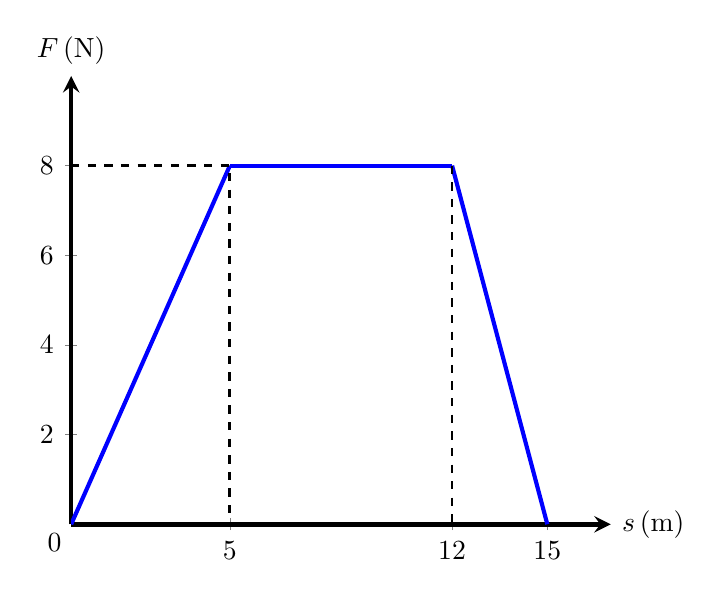
\begin{tikzpicture}  
				\begin{axis}[  ultra thick,
					xmin=0,  
					xmax=17,  
					xtick={0,5,12,15},
					ytick={0,2,...,8},
					ymin=0,  
					ymax=10, 
					samples=300,
					axis lines=center, 
					xlabel=$\xsi{s}{\left(\si{\meter}\right)}$, 		ylabel=$\xsi{F}{\left(\si{\newton}\right)}$,
					every axis y label/.style={at=(current axis.above origin),anchor=south},  
					every axis x label/.style={at=(current axis.right of origin),anchor=west},  ]
					\addplot [line width=1.5pt, blue, smooth, domain=0:5] {1.6*x};  
					\addplot [line width=1.5pt, blue, smooth, domain=5:12] {8}; 
					\addplot [line width=1.5pt, blue, smooth, domain=12:15] {8-8*(x-12)/3}; 
					\draw[dashed, line width=1pt] (axis cs: 0,8)--(axis cs:5,8)--(axis cs:5,0);
					\draw[dashed, line width=1pt] (axis cs:12,8)--(axis cs:12,0);
					\coordinate (O) at (axis cs: 0,0);
				\end{axis}  
				\node[below left] at (O) {0};
			\end{tikzpicture}
		\end{center}
		\begin{enumerate}[label=\alph*)]
			\item Tính công của lực $\vec{F}$.
			\item Tìm vận tốc của vật tại vị trí ứng với điểm cuối của đồ thị.
		\end{enumerate}
		\loigiai{
			\begin{enumerate}[label=\alph*)]
				\item $A=\SI{88}{\joule}$.
				\item $v=\sqrt{\dfrac{2A}{m}}\approx\SI{9.38}{\meter/\second}$.
			\end{enumerate}
		}
	\end{ex}
	% ======================================================================
	\begin{ex}\mkstar{3}
		Một ô tô có khối lượng $m=\SI{1.20}{\text{tấn}}$ chuyển động lên trên một con dốc phẳng có độ dài $s=\SI{1.50}{\kilo\meter}$ với vận tốc $v=\SI{54.0}{\kilo\meter/\hour}$. Chiều cao của đỉnh dốc so với mặt phẳng nằm ngang đi qua chân dốc (gốc thế năng nằm ở chân dốc) là $h=\SI{30.0}{\meter}$.
		Biết gia tốc rơi tự do là $g=\SI{9.8}{\meter/\second^2}$.
		\begin{enumerate}[label=\alph*)]
			\item Tính thế năng của ô tô ở đỉnh con dốc.
			\item Lấy gốc thời gian là lúc ô tô ở chân dốc, tìm thời điểm thế năng của ô tô bằng $\varepsilon=\SI{25}{\percent}$ thế năng của nó tại đỉnh dốc.
			\item Xác định công suất của động cơ ô tô biết rằng tỉ số giữa thế năng của ô tô với công mà động cơ của nó thực hiện là $\eta=\SI{90.0}{\percent}$.
		\end{enumerate}
		\loigiai{
		\begin{enumerate}[label=\alph*)]
			\item Thế năng của ô tô khi nó ở đỉnh dốc:
			$$W_{\text{th}}=mgh\approx\SI{353}{\kilo\joule}.$$
			\item Ta có:
			$$\dfrac{W_{\text{t}}}{W_{\text{th}}}=\dfrac{mgh_{\text{t}}}{mgh}=\dfrac{h_{\text{t}}}{h}=\dfrac{s_{\text{t}}}{s_{\text{h}}}=\dfrac{vt}{s}=\varepsilon$$
			Trong đó $h_{\text{t}}$ là độ cao của ô tô (so với chân dốc) ở thời điểm $t$, $s_{\text{t}}$ là quãng đường ô tô đi được trong khoảng thời gian $t=\dfrac{\varepsilon s}{v}=\SI{25.0}{\second}$.
			\item Ta có:
			$$\eta=\dfrac{W_{\text{t}}}{A}=\dfrac{mgh_{\text{t}}}{\calP t}$$
			Từ câu b, ta có:
			$$h_{\text{t}}=\dfrac{hvt}{s}\Rightarrow \eta=\dfrac{mg}{\calP t}\cdot\dfrac{hvt}{s}=\dfrac{mghv}{\calP s}.$$
			Công suất của động cơ ô tô:
			$$\calP=\dfrac{mghv}{\eta s}=\SI{3.92}{\kilo\watt}.$$
		\end{enumerate}
		}
	\end{ex}
% ======================================================================
\begin{ex}\mkstar{3}
Một vật có khối lượng $m=\SI{1.00}{\kilogram}$ được thả rơi không vận tốc đầu từ độ cao $h=\SI{10.0}{\meter}$ so với mặt đất. Vật dừng lại sau khi ngập sâu vào lòng đất đoạn $d=\SI{30.0}{\centi\meter}$ theo phương thẳng đứng. Biết rằng gia tốc rơi tự do là $g=\SI{9.80}{\meter/\second^2}$. Lấy gốc thế năng là mặt đất. Tính:
\begin{enumerate}[label=\alph*)]
	\item thế năng cực tiểu của vật trong quá trình chuyển động;
	\item công mà mặt đất truyền cho vật.
\end{enumerate}	
	\loigiai{
	\begin{enumerate}[label=\alph*)]
		\item Thế năng của vật đạt giá trị cực tiểu khi nó ở độ sâu cực đại:
		$$W_{\text{t min}}=-mgd=\SI{-2.94}{\joule}.$$
		\item Công mà mặt đất truyền cho vật, áp dụng định lý động năng:
		$$0-\dfrac{1}{2}mv^2=A_{\vec{P}}+A_{\vec{F}_c}\Rightarrow A_{\vec{F}_c}=-\dfrac{1}{2}mv^2-A_{\vec{P}}$$
		$$\Rightarrow A_{\vec{F}_c}=-mgh-mgd=-mg(h+d)\approx\SI{-101}{\joule}.$$
	\end{enumerate}
	}
\end{ex}
\Closesolutionfile{ans}
					\let\lesson\undefined
\newcommand{\lesson}{\phantomlesson{Bài 17: Động năng và thế năng. Định luật bảo toàn cơ năng}}
\chapter[Định luật bảo toàn cơ năng.]{Định luật bảo toàn cơ năng}
\setcounter{section}{0}
\section{Lý thuyết}
\subsection{Cơ năng của một vật chuyển động trong trọng trường}
Cơ năng của vật chuyển động dưới tác dụng của trọng lực bằng tổng động năng và thế năng trọng trường của vật.\\
Kí hiệu cơ năng của vật là $W$:
\begin{equation*}
	W=W_\text{đ}+W_\text{t}=\dfrac{1}{2}mv^2+mgz\label{CT-conang},
\end{equation*}
trong đó:
\begin{itemize}
	\item $W$ là cơ năng của vật;
	\item $W_\text{đ}=\dfrac{1}{2}mv^2$ là động năng của vật;
	\item $W_\text{t}=mgz$ là thế năng của vật.
\end{itemize}
\subsection{Bảo toàn cơ năng của vật chuyển động trong trọng trường}
Khi một vật chuyển động trong trọng trường chỉ chịu tác dụng của trọng lực thì cơ năng của vật là một đại lượng bảo toàn.
\begin{equation*}
	W=W_\text{đ}+W_\text{t}=\dfrac{1}{2}mv^2+mgz=\textrm{hằng số}
\end{equation*}
\textit{Hệ quả:}
\begin{itemize}
	\item Nếu động năng giảm thì thế năng tăng (động năng chuyển hóa thành thế năng) và ngược lại.
	\item Tại vị trí nào động năng cực đại thì thế năng cực tiểu và ngược lại.
\end{itemize}
\subsection{Biến thiên cơ năng}
Khi một vật chuyển động trong trọng trường, nếu vật chịu tác dụng thêm lực cản (không phải lực thế) thì cơ năng của vật sẽ biến đổi. Công của lực cản bằng độ biến thiên của cơ năng.
\begin{equation*}
	A=W_2-W_1,
\end{equation*}
trong đó:
\begin{itemize}
	\item $A$ là công của lực cản;
	\item $W_1$ là cơ năng lúc đầu;
	\item $W_2$ là cơ năng lúc sau.
\end{itemize}
\section{Mục tiêu bài học - Ví dụ minh họa}
\begin{dang}{Biện luận sự chuyển hóa giữa động năng và thế năng}
	
	\viduii{2}{
		Một vật có khối lượng $m=\SI{1}{kg}$ được thả rơi tự do từ độ cao $\SI{20}{m}$ so với mặt đất. Chọn gốc thế năng tại mặt đất. Bỏ qua mọi ma sát. Ngay khi vật chạm đất thì
		\begin{mcq}(1)
			\item động năng cực đại, thế năng cực tiểu.
			\item động năng bằng thế năng.
			\item động năng cực tiểu, thế năng cực đại.
			\item động năng bằng một nửa thế năng.
		\end{mcq}
	}
	{\hide{Trong quá trình rơi, vận tốc của vật tăng dần còn độ cao giảm dần. Do đó, khi vật chạm đất thì vận tốc lớn nhất nên động năng cực đại, còn độ cao nhỏ nhất nên thế năng cực tiểu.
			
			\textbf{Đáp án: A}.}
		
	}
	\viduii{2}{
		Một vật có khối lượng $m=\SI{1}{kg}$ được ném lên với vận tốc $\SI{10}{m/s}$ từ độ cao $\SI{1}{m}$ so với mặt đất. Chọn gốc thế năng tại mặt đất. Bỏ qua mọi ma sát. Ngay khi vật lên đến độ cao cực đại thì
		\begin{mcq}(1)
			\item động năng cực đại, thế năng cực tiểu.
			\item động năng bằng thế năng.
			\item động năng cực tiểu, thế năng cực đại.
			\item động năng bằng một nửa thế năng.
		\end{mcq}
	}
	{
	\hide{	Trong quá trình vật bay lên, vận tốc giảm dần còn độ cao tăng dần. Do đó, khi vật lên đến độ cao cực đại thì thế năng cực đại vì độ cao cực đại, còn động năng cực tiểu vì vận tốc cực tiểu.
		
		\textbf{Đáp án: C}.}
	}
\end{dang}
\begin{dang}{Xác định cơ năng của vật chuyển động trong trọng trường}
	\viduii{2}{Một vật có khối lượng $\SI{2}{kg}$ rơi tự do không vận tốc đầu từ độ cao $\SI{5}{m}$ xuống mặt đất. Nếu chọn gốc thế năng tại mặt đất, lấy $g=\SI{10}{m/s^2}$, cơ năng của vật có giá trị 
		\begin{mcq}(4)
			\item $\SI{10}{J}$.
			\item $\SI{100}{J}$.
			\item $\SI{50}{J}$.
			\item $\SI{5}{J}$.
		\end{mcq}
	}
	{\hide{Cơ năng của vật bằng tổng động năng và thế năng. Tại thời điểm bắt đầu rơi, vận tốc của vật bằng không, giá trị cơ năng tương ứng là: 
			\begin{align*}
				W&=W_\text{đ}+W_\text{t}\\
				&=\dfrac{1}{2}mv^2+mgh\\
				&=\dfrac{1}{2}\cdot\SI{2}{\kilogram}\cdot(\SI{0}{\meter/\second})^2+\SI{2}{\kilogram}\cdot\SI{10}{\meter/\second^2}\cdot\SI{5}{\meter}\\
				&=\SI{100}{\joule}.
			\end{align*}
			
			\textbf{Đáp án: B.}}
	
	}
	\viduii{3}{Một vật có khối lượng $\SI{100}{\gram}$ được ném thẳng đứng từ độ cao $\SI{5}{\meter}$ lên phía trên với vận tốc đầu là $\SI{10}{\meter/\second}$. Bỏ qua lực cản của không khí. Lấy $g=\SI{10}{\meter/\second^2}$. Xác định cơ năng của vật ở thời điểm $\SI{0,5}{\second}$ kể từ khi chuyển động.
	}
	{\hide{Với lưu ý rằng vật chuyển động trong trọng trường và bỏ qua lực cản thì cơ năng của hệ được bảo toàn. Do đó cơ năng của vật ở thời điểm \SI{0.5}{\second} cũng bằng với cơ năng ở thời điểm ban đầu, và có giá trị: 
			\begin{align*}
				W=\dfrac{1}{2}mv_0^2+mgz_0=\dfrac{1}{2}\cdot\SI{0.1}{\kilogram}\cdot(\SI{10}{\meter/\second})^2+\SI{0.1}{\kilogram}\cdot\SI{10}{\meter/\second^2}\cdot\SI{5}{\meter}=\SI{10}{\joule}.
		\end{align*}}
	}
\end{dang}


\begin{dang}{Áp dụng định luật bảo toàn cơ năng cho vật rơi tự do }
	\viduii{2}{Một vật được ném theo phương thẳng đứng hướng xuống từ độ cao $\SI{15}{m}$ so với mặt đất với tốc độ $\SI{10}{m/s}$. Bỏ qua mọi lực cản. Chọn gốc thế năng tại mặt đất. Lấy $g=\SI{10}{m/s^2}$. Tốc độ của vật khi vật vừa chạm đất là
		\begin{mcq}(4)
			\item $\SI{10}{m/s}$.
			\item $\SI{15}{m/s}$.
			\item $\SI{20}{m/s}$.
			\item $\SI{400}{m/s}$.
		\end{mcq}
	}
	{\hide{
			Cơ năng của vật ở thời điểm đầu (khi vừa ném)
			\begin{align*}
				W_1=\dfrac{1}{2}mv_0^2+mgz_0
			\end{align*}
			Cơ năng của vật ở thời điểm cuối (khi chạm đất $z=0$)
			\begin{align*}
				W_2=\dfrac{1}{2}mv^2+mgz=\dfrac{1}{2}mv^2
			\end{align*}
			Bảo toàn cơ năng lúc vừa ném và lúc vừa chạm đất:
			\begin{eqnarray*}
				&&W_1=W_2\\
				&\Leftrightarrow&\dfrac{1}{2}mv_0^2+mgz_0=\dfrac{1}{2}mv^2\\
				&\Rightarrow& v=\sqrt{v_0^2+2gz_0}=\sqrt{(\SI{10}{\meter/\second})^2+2\cdot\SI{10}{\meter/\second^2}\cdot\SI{15}{\meter}}=\SI{20}{\meter/\second}.
			\end{eqnarray*}
			\textbf{Đáp án: C.}}
	}
	\viduii{2}{Một vật được thả rơi tự do từ độ cao $\SI{3}{\meter}$. Xác định độ cao của vật khi động năng bằng hai lần thế năng.
	}
	{\hide{Chọn mốc thế năng tại mặt đất.\\
			Tại vị trí thả, vật không có vận tốc nên động năng bằng không, cơ năng đúng bằng thế năng
			\begin{equation*}
				W_1=W_\text{đ1}+W_\text{t1}=0+W_\text{t1}=mgz_1.
			\end{equation*}
			Cơ năng của vật khi động năng bằng hai lần thế năng:
			\begin{equation*}
				W_2=W_\text{đ2}+W_\text{t2}=2W_\text{t2}+W_\text{t2}=3W_\text{t2}=3mgz_2.
			\end{equation*}	
			Áp dụng định luật bảo toàn cơ năng:
			\begin{eqnarray*}
				&&W_1=W_2\\
				&\Leftrightarrow& mgz_1 = 3mgz_2\\
				&\Rightarrow& z_2 = \dfrac{1}{3}z_1\\
				&\Rightarrow&z_2 =\dfrac{1}{3}\cdot \SI{3}{\meter}=\SI{1}{\meter}.
		\end{eqnarray*}}
	}
	\viduii{3}{
		Một vật ném thẳng đứng xuống dưới đất từ độ cao $\SI{5}{\meter}$. Khi chạm đất vật nảy lên với độ cao $\SI{7}{\meter}$. Bỏ qua mất mát năng lượng khi va chạm và sức cản môi trường. Lấy $g=\SI{10}{\meter/\second^2}$. Vận tốc ném ban đầu có giá trị bằng bao nhiêu?
	}
	{\hide{Chọn mốc thế năng tại mặt đất.\\
			Cơ năng của vật tại vị trí thả là:
			\begin{equation*}
				W_1=W_\text{đ1}+W_\text{t1}=\dfrac{1}{2}mv_1^2+mgz_1.
			\end{equation*}
			Cơ năng của vật tại vị trí vật nảy lên với độ cao $\SI{7}{\meter}$ là:
			\begin{equation*}
				W_2=W_\text{đ2}+W_\text{t2}=W_\text{t2}=mgz_2.
			\end{equation*}	
			Áp dụng định luật bảo toàn cơ năng:
			\begin{eqnarray*}
				&&W_1=W_2\\
				&\Leftrightarrow& \dfrac{1}{2}mv_1^2+mgz_1 = mgz_2\\
				&\Leftrightarrow& \dfrac{1}{2}v_1^2+gz_1 = gz_2\\
				&\Rightarrow& v_1 = \sqrt{2g(h_2-h_1)}\\
				&\Leftrightarrow& v_1 = \sqrt{2\cdot\SI{10}{\meter/\second^2}\cdot(\SI{7}{\meter}-\SI{5}{\meter})}\\
				&\Rightarrow& v_1 = 2\sqrt{10}\,\text{m/s}.
		\end{eqnarray*}}
	}
\end{dang}

\begin{dang}{Áp dụng định luật bảo toàn cơ năng cho con lắc đơn}
	
	\viduii{3}{
		Một con lắc đơn gồm sợi dây nhẹ không dãn, chiều dài $\SI{50}{cm}$, một đầu cố định, đầu còn lại treo vật nặng có khối lượng $\SI{100}{g}$. Ban đầu vật nặng đứng yên ở vị trí cân bằng. Tại vị trí này, truyền cho vật nặng vận tốc $v_0=\SI{5}{m/s}$ theo phương ngang. Chọn gốc thế năng tại vị trí cân bằng và cho $g=\SI{10}{m/s^2}$.
		\begin{enumerate}[label=\alph*)]
			\item Tìm cơ năng của vật.
			\item Khi vật lên đến vị trí M có dây treo hợp với phương thẳng đứng góc $\alpha_\text M$, vật có thế năng bằng $1/4$ động năng. Hãy tính $\alpha_\text M$ và vận tốc của vật tại M.
		\end{enumerate}
	}
	{\hide{	\begin{enumerate}[label=\alph*)]
				\item 			
				Cơ năng của vật bằng tổng động năng và thế năng:
				$$W_1 = \dfrac{1}{2}mv_1^2 + mgz_1 = \dfrac{1}{2}mv_1^2 + 0 = \SI{1.25}{J}.$$
				
				\item Trong quá trình chuyển động, vật chịu tác dụng của trọng lực là lực thế, và lực căng dây luôn vuông góc với quỹ đạo là lực không sinh công. 
				Do đó cơ năng của vật đươc bảo toàn. \\
				Khi thế năng bằng $1/4$ động năng thì động năng gấp 4 lần thế năng, cơ năng khi đó có thể tính theo công thức: 
				\begin{align*}
					W_2 = W_\text{đ2} + W_\text{t2} = 4 W_\text{t2} + W_\text{t2} = 5 W_\text{t2} 
				\end{align*}
				Áp dụng định luật bảo toàn cơ năng, ta tính được độ cao của điểm M:
				\begin{align*}
					W_2= W_1 \quad\Rightarrow\quad 5mgz_2 = \dfrac{1}{2}mv_1^2 \quad \Rightarrow \quad z_2 = \dfrac{1}{10}\dfrac{v_1^2}{g}=\SI{0.25}{m}.
				\end{align*}
				Góc $\alpha_\text M$ giữa phương thẳng đứng và phương dây treo được tính theo công thức: $\cos \alpha_\text M = \dfrac{l-z_2}{l} = \dfrac{1}{2}$, suy ra $\alpha_\text M = 60^\circ$.
				
				Vận tốc của vật tại M:
				$$W_\text{đ2} = 4 W_\text{t2} \Rightarrow \dfrac{1}{2}mv_2^2 = 4 mgz_2 \Rightarrow v_2 = \xsi{2\sqrt 5}{m/s}.$$
		\end{enumerate}}
		
	}
	\viduii{3}{
		Một dây nhẹ dài $l=\SI{1}{m}$ đầu trên cố định, đầu dưới treo một vật nặng khối lượng $m$. Người ta kéo cho dây treo lệch một góc $\alpha = 60^\circ$ so với phương thẳng đứng rồi thả nhẹ cho vật chuyển động. Lấy $g=\SI{10}{m/s^2}$. Bỏ qua lực cản của không khí.
		\begin{enumerate}[label=\alph*)]
			\item Xác định vận tốc vật khi vật đi qua vị trí mà dây treo hợp với phương thẳng đứng một góc $\beta = 30^\circ$.
			\item Chứng minh rằng tại vị trí dây treo thẳng đứng vận tốc của vật có độ lớn cực đại, tìm giá trị cực đại đó.
		\end{enumerate}
	}
	{\hide{\begin{enumerate}[label=\alph*)]
				\item Xác định vận tốc vật khi vật đi qua vị trí mà dây treo hợp với phương thẳng đứng một góc $\beta = 30^\circ$.
				
				Chọn gốc thế năng tại vị trí cân bằng của vật. Áp dụng định luật bảo toàn cơ năng:
				$$W_1 = W_2 \Rightarrow mgl(1-\cos \alpha) + 0 = \dfrac{1}{2} mv_2^2 + mgl (1-\cos \beta) \Rightarrow v_2 = \SI{2.7}{m/s}.$$
				
				\item Chứng minh rằng tại vị trí dây treo thẳng đứng vận tốc của vật có độ lớn cực đại, tìm giá trị cực đại đó.
				
				Tại vị trí dây treo thẳng đứng thì thế năng $z_3=0$, do đó động năng cực đại, dẫn đến vận tốc cực đại.
				
				Áp dụng bảo toàn cơ năng:
				$$W_1 = W_3 \Rightarrow mgl(1-\cos \alpha) = \dfrac{1}{2}mv_3^2 \Rightarrow v_3 = \xsi{\sqrt{10}}{m/s}.$$
		\end{enumerate}}
		
	}
\end{dang}

\begin{dang}{Áp dụng định luật bảo toàn năng lượng cho bài toán vật chịu tác dụng của lực không thế}
	\viduii{3}{Một vật có khối lượng $m=\SI{1}{\kilogram}$ rơi không vận tốc đầu từ độ cao $z_1$ so với mặt đất trong không khí,  lấy gia tốc trọng trường $g=\SI{10}{\meter/\second^2}$. Khi vật đi được $\SI{3}{\meter}$, biết lực cản trung bình của không khí ngược chiều với chuyển động và có độ lớn $\SI{4}{\newton}$, thì độ lớn vận tốc của vật là
		\begin{mcq}(4)
			\item $\SI{4,0}{\meter/\second}$.
			\item $\SI{7,7}{\meter/\second}$.
			\item $\SI{8,9}{\meter/\second}$.
			\item $\SI{6,0}{\meter/\second}$.
		\end{mcq}
	}
	{\hide{\begin{center}
				\includegraphics[scale=0.6]{../figs/VN10-PH-33-L-025-3-H1.jpg}
			\end{center}
			Công của lực cản khi vật chuyển động $\SI{3}{\meter}$ là:
			\begin{equation*}
				A=F_\text{c}S\cos\alpha=\SI{4}{\newton}\cdot\SI{3}{\meter}\cdot\cos(180^\circ)=\SI{-12}{\joule}.
			\end{equation*}
			Cơ năng của vật lúc bắt đầu rơi là:
			\begin{equation*}
				W_1=W_\text{đ1}+W_\text{t1}=\dfrac{1}{2}mv_1^2+mgz_1=mgz_1.
			\end{equation*}
			Cơ năng của vật sau khi rơi quãng đường $\SI{3}{\meter}$ là:
			\begin{equation*}
				W_2=W_\text{đ2}+W_\text{t2}=\dfrac{1}{2}mv_2^2+mgz_2.
			\end{equation*}
			Do vật chịu tác dụng thêm lực cản nên cơ năng vật biến đổi. Công của lực cản bằng độ biến thiên cơ năng:
			\begin{eqnarray*}
				&&A=W_2-W_1\\
				&\Rightarrow& A = \dfrac{1}{2}mv_2^2+mgz_2 - mgz_1\\
				&\Rightarrow& A= \dfrac{1}{2}mv_2^2+mg(z_2-z_1)\\
				&\Rightarrow& \SI{-12}{\joule} = \dfrac{1}{2}\cdot\SI{1}{\kilogram}\cdot v_2^2 + \cdot\SI{1}{\kilogram}\cdot \SI{10}{\meter/\second^2}\cdot(-\SI{3}{\meter})\\
				&\Rightarrow& v_2 = \SI{6}{\meter/\second}.
			\end{eqnarray*}
			\textbf{Đáp án: D.}}
	}
	\viduii{3}{Một vật có khối lượng $m$ bắt đầu trượt không vận tốc đầu từ đỉnh của một mặt phẳng nghiêng có hệ số ma sát $\mu=0,2$, góc nghiêng $\beta=30^\circ$, $g=\SI{10}{\meter/\second^2}$. Khi vật trượt được quãng đường dài $\SI{10}{\meter}$ trên mặt phẳng nghiêng thì vận tốc của vật là
		\begin{mcq}(4)
			\item $\SI{8}{\meter/\second}$.
			\item $\SI{7}{\meter/\second}$.
			\item $\SI{9}{\meter/\second}$.
			\item $\SI{10}{\meter/\second}$.
		\end{mcq}
	}
	{\hide{\textbf{Cách 1:}\\
			\begin{center}
				\includegraphics[scale=0.5]{../figs/VN10-PH-33-L-025-3-H2.jpg}
			\end{center}
			Chọn O$x$ và O$y$ như hình vẽ.\\
			Các lực tác dụng gồm:
			\begin{itemize}
				\item Lực ma sát $\vec{F}_\text{ms}$;
				\item Trọng lực $\vec{P}$;
				\item Phản lực $\vec{N}$.
			\end{itemize}
			Áp dụng định luật II Newton ta được:
			\begin{equation*}
				\vec{a}=\dfrac{\vec{P}+\vec{N}+\vec{F}_\text{ms}}{m}.
			\end{equation*}
			Chiếu lên O$y$ ta được:
			\begin{equation*}
				N = P\cos\beta = mg\cos\beta.
			\end{equation*}
			Chiếu lên O$x$ ta được:
			\begin{equation*}
				a=\dfrac{P\sin\beta-F_\text{ms}}{m}=\dfrac{mg\sin\beta-\mu mg\cos\beta}{m}=g(\sin\beta-\mu\cos\beta).
			\end{equation*}
			Thay số vào ta được:
			\begin{equation*}
				a=g(\sin\beta-\mu\cos\beta)=\SI{10}{\meter/\second^2}\cdot (\sin30^\circ-0,2\cdot\cos30^\circ)=\SI{3,27}{m/s^2}.
			\end{equation*}
			Theo công thức liên hệ $a$, $v$, $s$ trong chuyển động thẳng biến đổi đều ta có:
			\begin{equation*}
				v^2-v_0^2=2as\Rightarrow v=\sqrt{v_0^2+2as}=\sqrt{2\cdot \left(\SI{3,27}{m/s^2}\right)\cdot \SI{10}{\meter}}= \SI{8}{\meter/\second}.
			\end{equation*}
			Vậy khi vật trượt được quãng đường dài $\SI{10}{\meter}$ trên mặt phẳng nghiêng thì vận tốc của vật là $\SI{8}{\meter/\second}$.\\
			\textbf{Cách 2:}\\
			\begin{center}
				\includegraphics[scale=0.5]{../figs/VN10-PH-33-L-025-3-H3.jpg}
			\end{center}
			Chọn mốc thế năng tại vị trí chân mặt phẳng nghiêng.\\
			Các lực tác dụng gồm:
			\begin{itemize}
				\item Lực ma sát $\vec{F}_\text{ms}$;
				\item Trọng lực $\vec{P}$;
				\item Phản lực $\vec{N}$.
			\end{itemize}
			Công của lực không thế tác dụng lên vật là:
			\begin{eqnarray*}
				A&=&A_\text{ms}+A_N\\
				&=&F_\text{ms}s\cos\alpha+0\\
				&=&\mu N s\cos\alpha\\
				&=&\mu\cdot  mg\cos\beta \cdot s \cdot \cos\alpha
			\end{eqnarray*}
			Cơ năng của vật lúc bắt đầu rơi là:
			\begin{equation*}
				W_1=W_\text{đ1}+W_\text{t1}=\dfrac{1}{2}mv_1^2+mgz_1=mgz_1.
			\end{equation*}
			Cơ năng của vật sau khi rơi quãng đường $\SI{10}{\meter}$ là:
			\begin{equation*}
				W_2=W_\text{đ2}+W_\text{t2}=\dfrac{1}{2}mv_2^2+mgz_2
			\end{equation*}
			Do vật chịu tác dụng thêm lực cản nên cơ năng vật biến đổi. Công của lực cản bằng độ biến thiên cơ năng:
			\begin{eqnarray*}
				A&=&W_2-W_1\\
				\Rightarrow A &=& \dfrac{1}{2}mv_2^2+mgz_2 - mgz_1\\
				\Rightarrow \mu\cdot  mg\cos\beta \cdot s \cdot \cos\alpha &=& \dfrac{1}{2}mv_2^2+mg(z_2 - z_1)\\
				\Rightarrow \mu\cdot  g\cos\beta \cdot s \cdot \cos\alpha &=& \dfrac{1}{2}v_2^2 - g s\sin\beta\\
				\Rightarrow 0,2 \cdot \SI{10}{\meter/\second^2} \cdot \cos 30^\circ \cdot \SI{10}{\meter} \cdot \cos 180^\circ &=& \dfrac{1}{2}\cdot v_2^2 -\SI{10}{\meter/\second^2}\cdot \SI{10}{\meter} \cdot\sin30^\circ\\
				\Rightarrow v_2 &=& \SI{8}{\meter/\second}.
			\end{eqnarray*}
			\textbf{Đáp án: A}.}
	}
	\viduii{3}{
		Một vật khối lượng $\SI{2}{kg}$ được ném thẳng đứng với vận tốc ban đầu $\SI{20}{m/s}$ xuống đất. Lấy $g=\SI{10}{m/s^2}$. Chọn gốc thế năng tại mặt đất. Bỏ qua lực cản của không khí trong quá trình vật chuyển động. Sau khi chạm đất, vật lún sâu $\SI{10}{cm}$ rồi dừng lại. Tính lực cản trung bình của đất.
	}
	{\hide{Cơ năng của vật tại ví trí ném:
			$$W_1 = W_\text{đ1} + W_\text{t1} = \SI{400}{J}.$$
			
			Cơ năng của vật tại vị trí sâu $\SI{10}{cm}$ dưới đất:
			$$W_2 = 0 + mgz_2 = \SI{-2}{J}.$$
			
			Khi vật dừng lại thì toàn bộ cơ năng chuyển thành công của lực cản của đất:
			$$\Delta W = W_2 - W_1 = \SI{-402}{J}= A_\text{cản} = -F_\text{cản} \cdot \SI{0.1}{m} \Rightarrow F_\text{cản} = \SI{4020}{N}.$$}
	}
	\viduii{3}{
		Ném vật khối lượng $\SI{150}{g}$ thẳng đứng lên cao từ mặt đất với vận tốc $\SI{20}{m/s}$. Cho $g=\SI{10}{m/s^2}$. Chọn gốc thế năng tại mặt đất.
		
		Nếu lực cản trung bình của không khí bằng $20\%$ trọng lượng của vật thì độ cao cực đại mà vật đạt được là bao nhiêu?
	}
	{\hide{Cơ năng:
			$$W_1 = W_\text{đ1} + 0 =\dfrac{1}{2}mv_0^2=\dfrac{1}{2}\cdot\SI{0.15}{\kilogram}\cdot(\SI{20}{\meter/\second})^2= \SI{30}{J}.$$
			Lực cản bằng trung bình của không khí tác dụng lên vật : $$F_\text{cản} = 20\%mg = 20\%\cdot\SI{0.15}{\kilogram}\cdot\SI{10}{\meter/\second^2}= \SI{0.3}{\newton}.$$
			Công của lực cản tác dụng lên vật từ khi vật ở mặt đất đến khi vật ở độ cao cực đại $h$:
			$$A_\text{cản} = -F_\text{cản} h.$$
			Độ biến thiên cơ năng bằng công của lực cản:
			$$\Delta W = W_2 - W_1 = mgh - W_1 = -F_\text{cản} h \Rightarrow h= \SI{16.67}{m}.$$}
	}
\end{dang}


					\let\lesson\undefined
\newcommand{\lesson}{\phantomlesson{Bài 17.}}
\setcounter{section}{2}
\section{Trắc nghiệm nhiều phương án lựa chọn}
\setcounter{ex}{0}
\Opensolutionfile{ans}[ans/VN10-2022-PH-TP027-TN]
% ===================================================================
\begin{ex}\mkstar{1}
Cơ năng là đại lượng	
	\choice
	{luôn luôn dương}
	{luôn luôn dương hoặc bằng 0}
	{\True có thể dương, âm hoặc bằng 0}
	{luôn luôn khác 0}
	\loigiai{}
\end{ex}
% ===================================================================
\begin{ex}\mkstar{1}
	Cơ năng của một vật được bảo toàn khi
	\choice
	{vật chịu tác dụng của các lực không phải là lực thế}
	{\True vật chỉ chịu tác dụng của lực thế}
	{vật chịu tác dụng của mọi lực bất kì}
	{vật chỉ chịu tác dụng của một lực duy nhất}
	\loigiai{}
\end{ex}
% ===================================================================
\begin{ex}\mkstar{1}
	Một vật được ném thẳng đứng lên cao, khi vật đạt độ cao cực đại thì tại đó
	\choice
	{động năng cực đại, thế năng cực tiểu}
	{\True động năng cực tiểu, thế năng cực đại}
	{động năng bằng thế năng}
	{động năng bằng nửa thế năng}
	\loigiai{}
\end{ex}
% ===================================================================
\begin{ex}\mkstar{2}
Từ độ cao $\SI{5.0}{\meter}$ so với mặt đất, người ta ném một vật khối lượng $\SI{200}{\gram}$ thẳng đứng lên cao với tốc độ ban đầu là $\SI{2}{\meter/\second}$. Bỏ qua lực cản của không khí. Lấy $g=\SI{10}{\meter/\second^2}$. Cơ năng của vật tại vị trí cao nhất mà vật đạt tới là
	\choice
	{$\SI{8.0}{\joule}$}
	{\True $\SI{10.4}{\joule}$}
	{$\SI{4.0}{\joule}$}
	{$\SI{16.0}{\joule}$}
	\loigiai{Do bỏ qua lực cản không khí nên cơ năng của vật bảo toàn:
		$$W=\dfrac{1}{2}mv^2_0+mgh=\dfrac{1}{2}\cdot\left(\SI{0.2}{\kilogram}\right)\cdot\left(\SI{2}{\meter/\second}\right)^2+\left(\SI{0.2}{\kilogram}\right)\cdot\left(\SI{10}{\meter/\second^2}\right)\cdot\left(\SI{5}{\meter}\right)=\SI{10.4}{\joule}.$$}
\end{ex}
% ===================================================================
\begin{ex}\mkstar{2}
	Một vận động viên trượt tuyết có tổng khối lượng $\SI{60}{\kilogram}$ bắt đầu trượt trên đồi tuyết từ điểm A đến điểm B. Biết điểm A có độ cao lớn hơn điểm B là $\SI{10}{\meter}$. Giả sử lực cản là không đáng kể. Lấy $g=\SI{10}{\meter/\second^2}$. Động năng của vận động viên này khi đến vị trí B là bao nhiêu?
	\choice
	{\True $\SI{6E3}{\joule}$}
	{$\SI{3E2}{\joule}$}
	{$\SI{60}{\joule}$}
	{Không xác định được vì còn phụ thuộc vào gốc thế năng}
	\loigiai{}
\end{ex}
%===================================================================
\begin{ex}\mkstar{2}
\immini{Ba quả bóng giống hệt nhau được ném ở cùng một độ cao từ đỉnh của toà nhà như bên. Quả bóng (1) được ném phương ngang, quả bóng (2) được ném xiên lên trên, quả bóng (3) được ném xiên xuống dưới. Các quả bóng được ném với cùng tốc độ ban đầu. Bỏ qua lực cản của không khí. Sắp xếp tốc độ của các quả bóng khi chạm đất theo thứ tự giảm dần.
	\choice
{1, 2, 3}
{2, 1, 3}
{3, 1, 2}
{\True Ba quả bóng chạm đất với cùng tốc độ}}
{\includegraphics[scale=0.4]{../figs/VN10-2022-PH-TP027-P-3}}
	\loigiai{}
\end{ex}

% ===================================================================
\begin{ex}\mkstar{3}
	Một con cá heo trong khi nhào lộn đã vượt khỏi mặt biển tới độ cao $\SI{5}{\meter}$. Nếu coi cá heo vượt lên khỏi mặt biển được chỉ nhờ động năng nó có vào lúc rời mặt biển và lấy $g=\SI{10}{\meter/\second^2}$ thì tốc độ của cá heo vào lúc rời mặt biển là
	\choice
	{\True $\SI{10}{\meter/\second}$}
	{$\SI{7.07}{\meter/\second}$}
	{$\SI{100}{\meter/\second}$}
	{$\SI{50}{\meter/\second}$}
	\loigiai{Áp dụng định luật bảo toàn cơ năng tại vị trí cá heo vừa rời mặt biển và vị trí nó có độ cao cực đại:
		$$W_\text{đ1}+W_\text{t1}=W_\text{đ2}+W_\text{t2}\Leftrightarrow \dfrac{1}{2}mv^2_0=mgh_\text{max}$$
		$$\Rightarrow v=\sqrt{2gh}=\SI{10}{\meter/\second}.$$}
\end{ex}
% ===================================================================
\begin{ex}\mkstar{3}
	Một vật khối lượng $\SI{400}{\gram}$ được thả rơi tự do từ độ cao $\SI{20}{\meter}$ so với mặt đất. Cho $g=\SI{10}{\meter/\second^2}$. Sau khi rơi được $\SI{12}{\meter}$, động năng của vật bằng
	\choice
	{$\SI{16}{\joule}$}
	{$\SI{24}{\joule}$}
	{$\SI{32}{\joule}$}
	{\True $\SI{48}{\joule}$}
	\loigiai{Động năng của vật sau khi rơi được $\SI{12}{\meter}$:
		$$W_\text{đ}=W-W_\text{t}=mgh_\text{max}-mgh=mgs=\left(\SI{0.4}{\kilogram}\right)\cdot\left(\SI{10}{\meter/\second^2}\right)\cdot\left(\SI{12}{\meter}\right)=\SI{48}{\joule}.$$}
\end{ex}
% ===================================================================
\begin{ex}\mkstar{3}
	Hòn đá được ném thẳng đứng lên với vận tốc $v_0=\SI{20}{\meter/\second}$ từ mặt đất. Chọn gốc thế năng tại mặt đất. Thế năng bằng $\dfrac{1}{4}$ động năng khi vật có độ cao
	\choice
	{$\SI{16}{\meter}$}
	{$\SI{5}{\meter}$}
	{\True $\SI{4}{\meter}$}
	{$\SI{20}{\meter}$}
	\loigiai{Áp dụng định luật bảo toàn cơ năng tại vị trí ban đầu và vị trí hòn đá có thế năng bằng $\dfrac{1}{4}$ động năng:
		$$W_\text{t}=\dfrac{1}{5}W\Leftrightarrow mgh=\dfrac{1}{5}\cdot\dfrac{1}{2}mv^2_0\Rightarrow h=\SI{4}{\meter}.$$}
\end{ex}
% ===================================================================
\begin{ex}\mkstar{3}
	Một quả bóng được thả rơi tự do từ độ cao $\SI{20}{\meter}$ so với mặt đất. Khi chạm đất, một phần cơ năng biến thành nhiệt năng nên quả bóng chỉ nảy lên theo phương thẳng đứng với độ cao $\SI{10}{\meter}$. Tỉ số tốc độ của quả bóng trước và sau khi chạm đất bằng
	\choice
	{2}
	{0,5}
	{\True $\sqrt{2}$}
	{$\dfrac{1}{\sqrt{2}}$}
	\loigiai{Tỉ số động năng của quả bóng trước và sau khi chạm đất:
		$$\dfrac{W_\text{đ}}{W'_\text{đ}}=\dfrac{mgh}{mgh'}=2$$
		$$\Leftrightarrow \dfrac{v^2}{v'^2}=2\Rightarrow v=\sqrt{2}v'.$$}
\end{ex}
% ===================================================================
\begin{ex}\mkstar{3}
Từ một đỉnh tháp cao $\SI{20}{\meter}$, người ta ném thẳng đứng lên cao một hòn đá khối lượng $\SI{50}{\gram}$ với tốc độ ban đầu $\SI{18}{\meter/\second}$. Khi rơi chạm mặt đất, tốc độ của hòn đá bằng $\SI{20}{\meter/\second}$. Lấy $g=\SI{10}{\meter/\second^2}$. Xác định công của lực cản do không khí tác dụng lên hòn đá.	
	\choice
	{\True $\SI{-8.1}{\joule}$}
	{$\SI{-11.9}{\joule}$}
	{$\SI{-9.95}{\joule}$}
	{$\SI{-8100}{\joule}$}
	\loigiai{Công của lực cản không khí tác dụng lên hòn đá bằng độ biến thiên cơ năng của hòn đá:
		\begin{eqnarray*}
			A_{F_c}&=&W_2-W_1=\dfrac{1}{2}mv^2_2-\dfrac{1}{2}mv^2_1-mgh\\
			&=&\dfrac{1}{2}\cdot\left(\SI{0.05}{\kilogram}\right)\cdot\left[\left(\SI{20}{\meter/\second}\right)^2-\left(\SI{18}{\meter/\second}\right)^2\right]-\left(\SI{0.05}{\kilo\gram}\right)\cdot\left(\SI{10}{\meter/\second^2}\right)\cdot\left(\SI{20}{\meter}\right)=\SI{-8.1}{\joule}.
	\end{eqnarray*}}
\end{ex}
% ===================================================================
\begin{ex}\mkstar{3}
Một con lắc đơn gồm vật nặng khối lượng $m = \SI{400}{\gram}$, dây treo không dãn có chiều dài $\ell=\SI{1.5}{\meter}$. Chọn mốc thế năng tại vị trí cân bằng của vật, lấy $g=\SI{10}{\meter/\second^2}$, ở góc lệch $\alpha=\SI{60}{\degree}$ so với phương thẳng đứng vật có tốc độ $v=\SI{2}{\meter/\second}$. Cơ năng của vật bằng	
	\choice
	{$\SI{0.8}{\joule}$}
	{$\SI{3.0}{\joule}$}
	{\True $\SI{3.8}{\joule}$}
	{$\SI{8.3}{\joule}$}
	\loigiai{Cơ năng của con lắc:
		\begin{eqnarray*}
			W&=&W_\text{t}+W_\text{đ}=mg\ell\left(1-\cos\alpha\right)+\dfrac{1}{2}mv^2\\
			&=&\left(\SI{0.4}{\kilogram}\right)\cdot\left(\SI{10}{\meter/\second^2}\right)\cdot\left(\SI{1.5}{\meter}\right)\cdot\left(1-\cos\SI{60}{\degree}\right)+\dfrac{1}{2}\cdot\left(\SI{0.4}{\kilogram}\right)\cdot\left(\SI{2}{\meter/\second}\right)^2=\SI{3.8}{\joule}.
	\end{eqnarray*}}
\end{ex}
% ===================================================================
\begin{ex}\mkstar{3}
Một con lắc đơn có chiều dài $\ell=\SI{1.6}{\meter}$. Kéo cho dây treo hợp với phương thẳng đứng một góc $\SI{60}{\degree}$ rồi thả nhẹ. Bỏ qua sức cản không khí. Lấy $g = \SI{10}{\meter/\second^2}$. Tốc độ của con lắc khi đi qua vị trí cân bằng là	
	\choice
	{$\SI{2.82}{\meter/\second}$}
	{$\SI{5.66}{\meter/\second}$}
	{\True $\SI{4.00}{\meter/\second}$}
	{$\SI{3.16}{\meter/\second}$}
	\loigiai{Áp dụng định luật bảo toàn cơ năng cho con lắc tại vị trí thả và lúc qua vị trí cân bằng (gốc thế năng ở vị trí cân bằng):
		$$mg\ell\left(1-\cos\alpha_0\right)=\dfrac{1}{2}mv^2\Rightarrow \left|v\right|=\sqrt{2g\ell\left(1-\cos\alpha_0\right)}=\SI{4}{\meter/\second}.$$}
\end{ex}


% ===================================================================
\begin{ex}\mkstar{3}
\immini{Hình bên biểu diễn sự phụ thuộc thế năng và động năng của một chất điểm rơi tự do theo thời gian $t$. Động năng của chất điểm tại thời điểm chất điểm có thế năng bằng $\SI{7}{\joule}$ là
\choice
{$\SI{2}{\joule}$}
{\True $\SI{4}{\joule}$}
{$\SI{6}{\joule}$}
{$\SI{3}{\joule}$}
}	
{\begin{tikzpicture}  
		\begin{axis}[  ultra thick,yscale=0.5,
			xmin=0,  
			xmax=7,  
			xtick=\empty,
			ytick={0,6,8},
			ymin=0,  
			ymax=14, 
			samples=300,
			xticklabels=\empty,
			xlabel=$\xsi{t}{\left(\si{\second}\right)}$, 		ylabel=$\xsi{W_{\text{đ}}, W_{\mathrm{t}}}{\left(\si{\joule}\right)}$,
			axis lines=center, 
			every axis y label/.style={at=(current axis.above origin),anchor=south},  
			every axis x label/.style={at=(current axis.right of origin),anchor=west},  ]
			\draw[line width=1pt, dashed] (axis cs: 0,8)--(axis cs: 3.266,8)--(axis cs: 3.266,0);
			\draw[line width=1pt, dashed] (axis cs: 0,6)--(axis cs: 4,6)--(axis cs: 4,0);
			\draw[line width=1pt, dashed] (axis cs: 0,12)--(axis cs: 5.6569,12)--(axis cs: 5.6569,0);
			\addplot [line width=1.5pt, red, smooth, domain=0:5.657] {12-3*x^2/8} node[above right] {$W_{\mathrm{t}}$};  
			\addplot [line width=1.5pt, blue, smooth, domain=0:5.657] {3*x^2/8} node[right] {$W_{\text{đ}}$}; 
			\coordinate (O) at (axis cs: 0,0);
		\end{axis}  
		\node[below left] at (O) {0};
\end{tikzpicture}}
	\loigiai{}
\end{ex}
% ===================================================================
\begin{ex}\mkstar{3}
	\immini{Một ô tô mô hình được thả nhẹ từ trạng thái nghỉ từ độ cao $h$ của một cái rãnh không ma sát. Rãnh được uốn thành đường tròn có đường kính $D$ ở phía cuối như trên hình bên. Ô tô này trượt trên rãnh được cả vòng tròn mà không bị rơi. Giá trị tối thiểu của $h$ là}{\includegraphics[scale=0.7]{../figs/VN10-2022-PH-TP027-P-1}}
	\choice
	{\True $\dfrac{5D}{4}$}
	{$\dfrac{3D}{2}$}
	{$\dfrac{5D}{2}$}
	{$\dfrac{5D}{3}$}
	\loigiai{
		Để ô tô vượt qua đường tròn:
		$$N=\dfrac{mv^2}{D/2}-mg\ge0\Rightarrow v^2\ge \dfrac{gD}{2}.$$
		Bảo toàn cơ năng:
		$$mgh=mgD+\dfrac{1}{2}mv^2\Rightarrow h=D+\dfrac{1}{2}\cdot\dfrac{v^2}{g}\ge D+\dfrac{D}{4}=\dfrac{5D}{4}.$$
	}
\end{ex}
\Closesolutionfile{ans}
\section{Trắc nghiệm đúng/sai}
\setcounter{ex}{0}
\Opensolutionfile{ans}[ans/VN10-2022-PH-TP027-TF]
% ===================================================================
\begin{ex}\mkstar{2}
\immini{Một con lắc đơn gồm một quả cầu nặng $\SI{0.025}{\kilogram}$ treo vào đầu dây dài như hình. Kéo con lắc đến vị trí M rồi thả ra. Bỏ qua mọi lực cản, xem như dây không co dãn và khối lượng của sợi dây không đáng kể. Lấy $g=\SI{10}{\meter/\second^2}$. Chọn gốc thế năng tại vị trí thấp nhất của con lắc.
\choiceTF[t]
{\True Trong quá trình chuyển động, cơ năng của con lắc được bảo toàn}
{\True Thế năng của quả cầu tại vị trí M là $\SI{0.06}{\joule}$}
{\True Khi quả cầu ở vị trí M thì thế năng của quả cầu cực đại}
{\True Tốc độ quả cầu ở vị trí O gần bằng $\SI{2.19}{\meter/\second}$}
}
{\includegraphics[scale=0.3]{../figs/VN10-2022-PH-TP027-P-4}}	
	
	\loigiai{}
\end{ex}
% ===================================================================
\begin{ex}\mkstar{3}
Một vật có khối lượng $\SI{0.5}{\kilogram}$ được thả rơi từ độ cao $\SI{25}{\meter}$. Chọn gốc thế năng ở mặt đất. Bỏ qua mọi ma sát. Lấy $g=\SI{10}{\meter/\second^2}$.	
	\choiceTF[t]
	{\True Thế năng của vật ở độ cao $\SI{15}{\meter}$ là $\SI{75}{\joule}$ và động năng của vật khi đó là $\SI{50}{\joule}$}
	{\True Khi động năng bằng thế năng, vật ở vị trí cách mặt đất $\SI{12.5}{\meter}$}
	{\True Khi thế năng bằng ba lần động năng thì vật có tốc độ bằng $\xsi{5\sqrt{5}}{\meter/\second}$}
	{\True Động năng của vật khi chạm đất là $\SI{125}{\joule}$}
	\loigiai{
	\begin{itemchoice}
		\itemch Đúng. Lúc bắt đầu thả, cơ năng của vật bằng thế năng: $W=W_{\text{t}\max}=\SI{125}{\joule}.$\\
		Thế năng của vật ở độ cao $\SI{15}{\meter}$: $W_{\mathrm{t}}=mgh_1=0,5\cdot10\cdot15=\SI{75}{\joule}$.\\
		Động năng của vật khi đó: $$W_{\text{đ}}=W-W_{\mathrm{t}}=125-75=\SI{50}{\joule}.$$
		\itemch Đúng. Khi vật có động năng bằng thế năng $\Rightarrow W=W_{\text{đ}}+W_{\text{t}}=2W_{\text{t}}\Rightarrow h=\dfrac{h_{\max}}{2}=\SI{12.5}{\meter}$.
		\itemch Đúng. Khi vật có thế năng bằng ba lần động năng $\Rightarrow W=4W_{\text{đ}}\Leftrightarrow v=\sqrt{\dfrac{gh_{\max}}{2}}=\xsi{5\sqrt{5}}{\meter/\second}.$
		\itemch Đúng. Khi vật chạm đất thì $h=0$ nên thế năng $W_{\text{t}}=0$, khi đó: $W_{\text{đ}}=W=\SI{125}{\joule}$.
	\end{itemchoice}
	}
\end{ex}
% ===================================================================
\begin{ex}\mkstar{3}
Tại nơi có gia tốc trọng trường $g=\SI{10}{\meter/\second^2}$, một khối đá có khối lượng $M=\SI{200}{\kilogram}$ rơi không vận tốc đầu từ độ cao $h_0=\SI{12}{\meter}$ vào một cọc bê tông làm cọc ngập sâu vào đất $\SI{25}{\centi\meter}$. Biết lực cản của đất tác dụng vào cọc luôn không đổi. 
	\choiceTF[t]
	{Trong quá trình khối đá rơi thì năng lượng của khối đá chỉ tồn tại dưới dạng động năng}
	{\True Thế năng ban đầu của khối đá bằng $\SI{E4}{\joule}$, nếu chọn gốc thế năng ở độ cao cách mặt đất $\SI{5}{\meter}$}
	{\True Khi khối đá rơi đến vị trí cách mặt đất $\SI{5}{\meter}$ thì khối đá có tốc độ bằng $\xsi{2\sqrt{35}}{\meter/\second}$}
	{Lực cản trung bình của đất tác dụng vào cọc bằng $\SI{96}{\kilo\newton}$}
	\loigiai{
	\begin{itemchoice}
		\itemch Sai. Trong quá trình khối đá rơi thì năng lượng khối đá gồm thế năng và động năng.
		\itemch Đúng. Chọn gốc thế năng ở độ cao cách mặt đất $\SI{5}{\meter}$ thì lúc đó thế năng bằng $W_{\mathrm{t}}=mgh=200\cdot10\cdot5=\SI{E4}{\joule}$.
		\itemch Đúng. Khi đá rơi cách mặt đất $\SI{5}{\meter}$ và chọn gốc thế năng tại vị trí này, áp dụng định luật bảo toàn cơ năng:
		$$mgh=\dfrac{1}{2}mv^2\Rightarrow v=\sqrt{2gh}=\sqrt{2\cdot10\cdot\left(12-5\right)}=\xsi{2\sqrt{35}}{\meter/\second}.$$
		\itemch Sai. Chọn gốc thế năng tại đầu cọc.\\
		Áp dụng định luật bảo toàn năng lượng:
		$$W_2-W_1=-F_cs\Leftrightarrow -mgs-mgh_0=-F_cs\Rightarrow F_c=\dfrac{mg(s+h_0)}{s}=\SI{98}{\kilo\newton}.$$
	\end{itemchoice}
	}
\end{ex}
% ===================================================================
\begin{ex}\mkstar{3}
	Tại một nơi có gia tốc trọng trường $g=\SI{10}{\meter/\second^2}$, thả một vật có khối lượng $\SI{5}{\kilogram}$ tại vị trí có thế năng trọng trường bằng $W_{\text{t1}}=\SI{600}{\joule}$, khi đến mặt đất thì thế năng của vật bằng $W_{\text{t2}}=\SI{-1000}{\joule}$. Bỏ qua mọi ma sát.
	\choiceTF[t]
	{Sau khi thả vật thì động năng tăng dần, cơ năng giảm dần}
	{\True Vật đã rơi từ độ cao $\SI{32}{\meter}$ so với mặt đất} 
	{Gốc thế năng đã chọn ở độ cao $\SI{10}{\meter}$ so với mặt đất}
	{Tốc độ của vật tại gốc thế năng là $\xsi{2\sqrt{15}}{\meter/\second}$}
	\loigiai{
	\begin{itemchoice}
		\itemch Sai. Cơ năng của vật không đổi.
		\itemch Đúng. Ta có $W_{\text{t1}}-W_{\text{t2}}=mg\Delta h\Rightarrow \Delta h=\dfrac{W_{\text{t1}}-W_{\text{t2}}}{mg}=\SI{32}{\meter}$.
		\itemch Sai. Tại vị trí gốc thế năng thì $h=0$.\\
		$$h_1=\dfrac{W_{\text{t1}}}{mg}=\SI{12}{\meter}.$$
		Gốc thế năng đã chọn ở độ cao $\SI{20}{\meter}$ so với mặt đất.
		\itemch Sai. Tốc độ của vật tại gốc thế năng: $v=\sqrt{2gh_1}=\xsi{4\sqrt{15}}{\meter/\second}$.
	\end{itemchoice}
	}
\end{ex}
\Closesolutionfile{ans}
\section{Tự luận}
\setcounter{ex}{0}
\Opensolutionfile{ans}[ans/VN10-2022-PH-TP027-TL]
% ======================================================================
\begin{ex}\mkstar{2}
	Người ta ném một quả bóng có khối lượng $m=\SI{200}{g}$ từ độ cao $\SI{2}{m}$ so với mặt đất lên cao với vận tốc $\SI{5}{m/s}$. Cho $g=\SI{10}{m/s^2}$. Chọn gốc thế năng tại mặt đất. Tính động năng, thế năng, cơ năng của quả bóng tại vị trí ném.
	\loigiai{Động năng:
		$$W_\text{đ} = \dfrac{1}{2}mv^2 = \SI{2.5}{J}.$$
		Thế năng:
		$$W_\text t = mgz = \SI{4}{J}.$$
		Cơ năng:
		$$W=W_\text{đ} + W_\text t = \SI{6.5}{J}.$$}
\end{ex}
% ======================================================================
\begin{ex}\mkstar{3}
	Ném thẳng đứng xuống dưới một vật khối lượng $\SI{200}{g}$ với vận tốc $\SI{5}{m/s}$ từ độ cao $\SI{1.5}{m}$ so với mặt đất. Bỏ qua mọi lực cản. Cho $g=\SI{10}{m/s^2}$. Tính động năng, thế năng và cơ năng của vật
	\begin{enumerate}[label=\alph*)]
		\item ngay lúc ném.
		\item ngay trước khi chạm đất.
	\end{enumerate}
	\loigiai{	\begin{enumerate}[label=\alph*)]
			\item Tính động năng, thế năng và cơ năng của vật ngay lúc ném.\\
			Động năng:
			$$W_\text{đ 1} = \dfrac{1}{2}mv_1^2 = \SI{2.5}{J}.$$
			Thế năng:
			$$W_\text{t 1} = mgz_1 = \SI{3}{J}.$$
			Cơ năng:
			$$W_1 = W_\text{đ 1} + W_\text{t 1} = \SI{5.5}{J}.$$
			\item Tính động năng, thế năng và cơ năng của vật ngay trước khi chạm đất.\\
			Khi chạm đất thì $z_2 = 0$, suy ra $W_\text{t 2} = 0$.\\
			Khi đó cơ năng bằng động năng và bằng cơ năng ban đầu:
			$$W_2 = W_\text{đ 2} = W_1 = \SI{5.5}{J}.$$
	\end{enumerate}}
\end{ex}
% ======================================================================
\begin{ex}\mkstar{2}
Một vật khối lượng $\SI{2}{kg}$ được ném thẳng đứng với vận tốc ban đầu $\SI{20}{m/s}$ xuống đất. Lấy $g=\SI{10}{m/s^2}$. Chọn gốc thế năng tại mặt đất. Bỏ qua lực cản của không khí trong quá trình vật chuyển động.
\begin{enumerate}[label=\alph*)]
	\item Tính cơ năng của vật lúc ném.
	\item Tìm vận tốc của vật khi chạm đất.
\end{enumerate}	
	\loigiai{\begin{enumerate}[label=\alph*)]
			\item Tính cơ năng của vật lúc ném.\\
			Cơ năng:
			$$W_1 = W_\text{đ 1} + W_\text{t 1} = \SI{400}{J}.$$
			\item Tìm vận tốc của vật khi chạm đất.\\
			Áp dụng bảo toàn cơ năng:
			$$W_1 = W_2 \Rightarrow \SI{400}{J} = \dfrac{1}{2}mv_2^2 + 0 \Rightarrow v_2 = \SI{20}{m/s}.$$
	\end{enumerate}}
\end{ex}
% ======================================================================
\begin{ex}\mkstar{2}
	Một vật có khối lượng $\SI{2}{kg}$ được thả rơi tự do từ độ cao $\SI{2.5}{m}$ so với mặt đất. Lấy $g=\SI{10}{m/s^2}$, bỏ qua mọi lực cản của không khí. Chọn gốc thế năng ở mặt đất. Xác định vận tốc của vật khi vật đạt đến vị trí có độ cao giảm đi một nửa.
	\loigiai{Tại vị trí có độ cao giảm đi một nửa thì $z_2=\dfrac{z_2}{2} = \SI{1.25}{m}$. Áp dụng bảo toàn cơ năng:
		$$W_1 = W_2 \Rightarrow 0 + mgz_1 = \dfrac{1}{2}mv_2^2 + mgz_2 \Rightarrow v_2 = \SI{5}{m/s}.$$}
\end{ex}
% ======================================================================
\begin{ex}\mkstar{2}
	Một vật trượt không vận tốc đầu từ đỉnh một mặt phẳng nghiêng cao $\SI{1.25}{m}$. Cho gia tốc rơi tự do $g=\SI{10}{m/s^2}$. Vật trượt không ma sát trên mặt phẳng nghiêng. Hãy tính vận tốc của vật tại chân mặt phẳng nghiêng.	
	\loigiai{Chọn gốc thế năng tại chân mặt phẳng nghiêng. Áp dụng bảo toàn cơ năng:
		$$W_1 = W_2 \Rightarrow 0 + mgz_1 = \dfrac{1}{2}mv_2^2 + 0 \Rightarrow v_2 = \SI{5}{m/s}.$$}
\end{ex}
% ======================================================================
\begin{ex}\mkstar{2}
	\immini{Một quả bóng nhỏ được ném với vận tốc ban đầu $\SI{4}{\meter/\second}$ theo phương nằm ngang ra khỏi mặt bàn ở độ cao $\SI{1}{\meter}$ so với mặt sàn. Lấy $g=\SI{9.8}{\meter/\second^2}$ và bỏ qua mọi ma sát. Tính tốc độ của quả bóng khi nó chạm mặt sàn.}
	{\includegraphics[scale=0.4]{../figs/VN10-2022-PH-TP027-P-2}}
	\loigiai{
	$v\approx\SI{5.97}{\meter/\second}$.
	}
\end{ex}
% ======================================================================
\begin{ex}\mkstar{3}
	Ném vật khối lượng $\SI{150}{g}$ thẳng đứng lên cao từ mặt đất với vận tốc $\SI{20}{m/s}$. Bỏ qua sức cản không khí. Cho $g=\SI{10}{m/s^2}$. Chọn gốc thế năng tại mặt đất.
	\begin{enumerate}[label=\alph*)]
		\item Tính động năng, cơ năng của vật tại vị trí ném.
		\item Tìm độ cao cực đại mà vật đạt được.
	\end{enumerate}
	\loigiai{\begin{enumerate}[label=\alph*)]
			\item Tính động năng, cơ năng của vật tại vị trí ném.\\
			Động năng:
			$$W_\text{đ 1} = \dfrac{1}{2}mv_1^2 = \SI{30}{J}.$$
			Cơ năng:
			$$W_1 = W_\text{đ 1} + 0 = \SI{30}{J}.$$
			\item Tìm độ cao cực đại mà vật đạt được.\\
			Độ cao cực đại mà vật đạt được:
			$$W_1 = W_3 \Rightarrow \SI{30}{J} = 0 + mgz_3 \Rightarrow z_3 = \SI{20}{m}.$$
	\end{enumerate}}
\end{ex}

% ======================================================================
\begin{ex}\mkstar{3}
	Một vật khối lượng $\SI{1}{kg}$ được ném từ mặt đất lên cao theo phương thẳng đứng với vận tốc ban đầu là $\SI{10}{m/s}$. Bỏ qua mọi lực cản của môi trường và lấy $g=\SI{10}{m/s^2}$.
	\begin{enumerate}[label=\alph*)]
		\item Tính cơ năng ban đầu.
		\item Khi vật lên đến độ cao bằng $2/3$ độ cao cực đại so với nơi ném thì vật có vận tốc bằng bao nhiêu?
	\end{enumerate}
	\loigiai{\begin{enumerate}[label=\alph*)]
			\item Tính cơ năng ban đầu.\\
			Cơ năng vật tại nơi ném:
			$$W_1=W_\text{đ} + W_\text{t} = \dfrac{1}{2}mv_1^2 + 0 = \SI{50}{J}.$$
			\item Khi vật lên đến độ cao bằng $2/3$ độ cao cực đại so với nơi ném thì vật có vận tốc bằng bao nhiêu?\\
			Bảo toàn cơ năng tại vị trí ném và tại vị trí vật có độ cao cực đại:
			$$W_1 = W_2 \Rightarrow \SI{50}{J} = 0 + mgz_2 \Rightarrow z_2 = \SI{5}{m}.$$
			Bảo toàn cơ năng tại vị trí ném và tại vị trí vật có độ cao bằng $2/3$ độ cao cực đại ($z_3=\SI{3.33}{m}$):
			$$W_1 = W_3 \Rightarrow \SI{50}{J} = \dfrac{1}{2}mv_3^2 + mgz_3 \Rightarrow v_3 \approx \SI{5.77}{m/s}.$$
	\end{enumerate}}
\end{ex}
% ======================================================================
\begin{ex}\mkstar{3}
	\immini{Trượt từ cầu trượt xuống nước là một trò chơi cảm giác mạnh được các bạn trẻ rất yêu thích trong công viên nước Đầm Sen vào những ngày hè nóng bức. Một học sinh có khối lượng $\SI{50}{kg}$ bắt đầu trượt không vận tốc đầu từ đỉnh cầu trượt ba chiều từ độ cao $h=\SI{10}{m}$ so với mặt nước. Giả thiết cầu trượt không ma sát, lấy $g=\SI{10}{m/s^2}$.}
	{\includegraphics[scale=0.7]{../figs/VN10-2022-PH-TP029-1.png}}
	\begin{enumerate}[label=\alph*)]
	\item Tính vận tốc của bạn học sinh khi vừa chạm mặt nước.
	\item Ở độ cao nào bạn học sinh có động năng bằng 2 lần thế năng?
	\end{enumerate}
	\loigiai{\begin{enumerate}[label=\alph*)]
			\item Tính vận tốc của bạn học sinh khi vừa chạm mặt nước.
			
			Chọn gốc thế năng tại mặt nước. Áp dụng bảo toàn cơ năng:
			$$W_1 = W_2 \Rightarrow 0 + mgz_1 = \dfrac{1}{2}mv_2^2 + 0 \Rightarrow v_2 = \xsi{10\sqrt 2}{m/s}.$$
			\item Ở độ cao nào bạn học sinh có động năng bằng 2 lần thế năng?
			
			Áp dụng bảo toàn cơ năng với $W_\text{đ 3} = 2 W_\text{t 3}$:
			$$W_1 = W_3 \Rightarrow W_1 = 2W_\text{t 3} + W_\text{t 3} = 3 mgz_3 \Rightarrow z_3 = \xsi{10/3}{m}.$$
	\end{enumerate}}
\end{ex}

% ======================================================================
\begin{ex}\mkstar{3}
Một con lắc đơn gồm sợi dây nhẹ không dãn, chiều dài $\SI{50}{cm}$, một đầu cố định, đầu còn lại treo vật nặng có khối lượng $\SI{100}{g}$. Ban đầu vật nặng đứng yên ở vị trí cân bằng. Tại vị trí này, truyền cho vật nặng vận tốc $v_0=\SI{5}{m/s}$ theo phương ngang. Chọn gốc thế năng tại vị trí cân bằng và cho $g=\SI{10}{m/s^2}$.
\begin{enumerate}[label=\alph*)]
	\item Tìm cơ năng của vật.
	\item Khi vật lên đến vị trí M có dây treo hợp với phương thẳng đứng góc $\alpha_\text M$, vật có thế năng bằng $1/4$ động năng. Hãy tính $\alpha_\text M$ và vận tốc của vật tại M.
\end{enumerate}	
	\loigiai{\begin{enumerate}[label=\alph*)]
			\item Tìm cơ năng của vật.
			
			Cơ năng của vật bằng tổng động năng và thế năng:
			$$W_1 = \dfrac{1}{2}mv_1^2 + mgz_1 = \dfrac{1}{2}mv_1^2 + 0 = \SI{1.25}{J}.$$
			
			\item Khi vật lên đến vị trí M có dây treo hợp với phương thẳng đứng góc $\alpha_\text M$, vật có thế năng bằng $1/4$ động năng. Hãy tính $\alpha_\text M$ và vận tốc của vật tại M.
			
			Khi thế năng bằng $1/4$ động năng thì động năng gấp 4 lần thế năng, vậy cơ năng là
			
			$$W_2 = W_\text{đ 2} + W_\text{t 2} = 4 W_\text{t 2} + W_\text{t 2} = 5 W_\text{t 2} = W_1 \Rightarrow 5mgz_2 = \SI{1.25}{J} \Rightarrow z_2 = \SI{0.25}{m}.$$
			
			Mà góc $\alpha_\text M$ giữa phương thẳng đứng và phương dây treo được tính theo công thức: $\cos \alpha_\text M = \dfrac{l-z_2}{l} = \dfrac{1}{2}$, suy ra $\alpha_\text M = 60^\circ$.
			
			Vận tốc của vật tại M:
			$$W_\text{đ 2} = 4 W_\text{t 2} \Rightarrow \dfrac{1}{2}mv_2^2 = 4 mgz_2 \Rightarrow v_2 = \xsi{2\sqrt 5}{m/s}.$$
	\end{enumerate}}
\end{ex}
% ======================================================================
\begin{ex}\mkstar{3}
	Thả rơi không vận tốc đầu một vật có khối lượng $m=\SI{200}{g}$ từ độ cao $h_0=\SI{5}{m}$ so với mặt đất. Lấy $g=\SI{10}{m/s^2}$ và bỏ qua mọi lực cản.
	\begin{enumerate}[label=\alph*)]
		\item Tính cơ năng của vật và tốc độ của vật khi vừa chạm đất.
		\item Tính thế năng và động năng của vật khi vật có động năng bằng 3 lần thế năng. Khi đó vật có tốc độ và độ cao bao nhiêu?
		\item Kể từ lúc thả, sau thời gian ngắn nhất bao lâu thì vật có thế năng bằng 3 lần động năng?
	\end{enumerate}
	\loigiai{\begin{enumerate}[label=\alph*)]
			\item Tính cơ năng của vật và tốc độ của vật khi vừa chạm đất.
			
			Cơ năng:
			$$W_1 = mgh_0 + 0 = \SI{10}{J}.$$
			
			Khi vật chạm đất:
			$$W_1 = W_2 \Rightarrow \SI{10}{J} = \dfrac{1}{2} mv_2^2 + 0 \Rightarrow v_2 = \SI{10}{m/s}.$$
			
			\item Tính thế năng và động năng của vật khi vật có động năng bằng 3 lần thế năng. Khi đó vật có tốc độ và độ cao bao nhiêu?
			
			Ta có $W_\text{đ 3} = 3 W_\text{t 3}$ nên $W_3 = 4 W_\text{t 3} = \SI{10}{J}$, suy ra $W_\text{t 3} = \SI{2.5}{J}$, $z_3 = \SI{1.25}{m}$.
			
			Và $W_\text{đ 3} = \SI{7.5}{J}$, $v_3 = \xsi{5\sqrt 3}{m/s}$.
			
			\item Kể từ lúc thả, sau thời gian ngắn nhất bao lâu thì vật có thế năng bằng 3 lần động năng?
			
			Khi $W_\text{t 4} = 3W_\text{đ 4}$ thì $W_4 = \dfrac{4}{3} W_\text{t 4} = \dfrac{4}{3} mgz_4$, suy ra $z_4 = \SI{3.75}{m}$.
			
			Quãng đường vật rơi được: $s=h_0-z_4 = \SI{1.25}{m}$. Áp dụng công thức:
			$$s=\dfrac{1}{2}gt^2 \Rightarrow t = \SI{5}{s}.$$
	\end{enumerate}}
\end{ex}
% ======================================================================
\begin{ex}\mkstar{3}
	Vật nặng $\SI{2}{kg}$ trượt không vận tốc đầu từ đỉnh A của cung AB là $1/4$ cung tròn bán kính $R=\SI{2.4}{m}$. Sau đó, vật tiếp tục trượt trên mặt ngang BC cách mặt đất độ cao $h=\SI{2}{m}$. Cho $g=\SI{10}{m/s^2}$. Bỏ qua ma sát.
	\begin{enumerate}[label=\alph*)]
		\item Tính vận tốc của vật tại C.
		\item Đến C vật rơi xuống đất với vector vận tốc ban đầu song song mặt phẳng ngang. Tính vận tốc của vật khi vật chạm đất.
	\end{enumerate}
	\begin{center}
		\includegraphics[scale=0.4]{../figs/VN10-2022-PH-TP029-4}
	\end{center}
	\loigiai{\begin{enumerate}[label=\alph*)]
			\item Tính vận tốc của vật tại C.
			
			Chọn gốc thế năng tại mặt đất (tại D).
			
			Độ cao điểm A là $z_\text{A} = h + R = \SI{4.4}{m}$.
			
			Độ cao điểm C là $z_\text{C} = h = \SI{2}{m}$.
			
			Áp dụng bảo toàn cơ năng tại A và C:
			$$W_\text{A} = W_\text{C} \Rightarrow 0 + mgz_\text A = \dfrac{1}{2}mv_\text{C}^2 + mgz_\text{C} \Rightarrow v_\text{C} = \xsi{4\sqrt 3}{m/s}.$$
			
			\item Đến C vật rơi ngang và rơi xuống đất. Tính vận tốc của vật khi vật chạm đất.
			
			Áp dụng bảo toàn cơ năng tại C và D, với $z_\text{D} = 0$:
			$$W_\text{C} = W_\text{D} \Rightarrow \dfrac{1}{2}mv_\text{C}^2 + mgz_\text{C} = \dfrac{1}{2} mv_\text{D}^2 + 0 \Rightarrow v_\text{D} = \xsi{2\sqrt{22}}{m/s}.$$
	\end{enumerate}}
\end{ex}
% ======================================================================
\begin{ex}\mkstar{3}
	Một viên đạn $\SI{30}{\gram}$ đang bay ngang với tốc độ $\SI{500}{\meter/\second}$ theo phương ngang thì đâm xuyên $\SI{12}{\centi\meter}$ vào một bức tường rắn rồi dừng lại.
	\begin{enumerate}[label=\alph*)]
		\item Tìm độ giảm cơ năng của viên đạn.
		\item Tìm độ lớn lực cản trung bình do bức tường tác dụng lên đạn.
	\end{enumerate}
	\loigiai{
		\begin{enumerate}[label=\alph*)]
			\item $\Delta W=\SI{3750}{\joule}$.
			\item $F_c\approx\SI{31250}{\newton}$.
		\end{enumerate}
	}
\end{ex}
% ======================================================================
\begin{ex}\mkstar{3}
	Một viên bi nhỏ khối lượng $\SI{200}{g}$ được ném thẳng đứng xuống dưới từ điểm O có độ cao $\SI{7}{m}$ so với mặt đất với tốc độ ban đầu $\SI{4}{m/s}$. Bỏ qua sức cản của không khí, lấy $g=\SI{10}{m/s^2}$.  Đất mềm, viên bi lún thẳng xuống mặt đất thêm một đoạn $\SI{10}{cm}$. Tính lực cản trung bình của đất tác dụng lên viên bi. Giải bài toán bằng phương pháp năng lượng.
	\loigiai{Cơ năng của vật tại ví trí ném:
		$$W_1 = W_\text{đ 1} + W_\text{t 1} = \SI{15.6}{J}.$$
		Cơ năng của vật tại vị trí sâu $\SI{10}{cm}$ dưới đất:
		$$W_2 = 0 + mgz_2 = \SI{-0.2}{J}.$$
		Khi vật dừng lại thì toàn bộ cơ năng chuyển thành công của lực cản của đất:
		$$\Delta W = W_2 - W_1 = \SI{-15.8}{J}= A_\text{cản} = -F_\text{c} \cdot \SI{0.1}{m} \Rightarrow F_\text{cản} = \SI{158}{N}.$$}
\end{ex}
% ======================================================================
\begin{ex}\mkstar{3}
		Một vật có khối lượng $\SI{2}{kg}$ được thả rơi tự do từ độ cao $\SI{2.5}{m}$ so với mặt đất. Lấy $g=\SI{10}{m/s^2}$, bỏ qua mọi lực cản của không khí. Chọn gốc thế năng ở mặt đất.\\
	Khi rơi đến mặt đất, vật va chạm với mặt đất và nảy lên đến độ cao cực đại là $\SI{2}{m}$. Tìm phần cơ năng đã mất đi sau khi vật va chạm với mặt đất.
	\loigiai{Cơ năng lúc thả vật (cơ năng trước khi vật va chạm với mặt đất):
		$$W_1 = mgz_1 = \SI{50}{J}.$$
		Cơ năng lúc vật nảy lên đến độ cao cực đại (cơ năng sau khi vật va chạm với mặt đất):
		$$W_2 = mgz_2 = \SI{40}{J}.$$
		Phần cơ năng đã mất đi: $$\Delta W = |W_2 - W_1| = \SI{10}{J}.$$}
\end{ex}

% ======================================================================
\begin{ex}\mkstar{3}
	Từ tầng 10 của tòa nhà cao tầng cách mặt đất $\SI{35}{m}$, một vật nặng $\SI{200}{g}$ được ném theo phương thẳng đứng, hướng xuống với tốc độ $\SI{20}{m/s}$. Chọn mốc thế năng tại mặt đất, bỏ qua mọi ma sát và lực cản của không khí, lấy $g=\SI{10}{m/s^2}$. Khi rơi xuống đất, do đất mềm và lún thì người ta thấy vật lún sâu vào đất một đoạn. Biết lực cản trung bình của đất là $\SI{440}{N}$. Tìm độ sâu vật lún vào đất.
	\loigiai{Cơ năng lúc ném vật:
		$$W_1 = \dfrac{1}{2}mv_1^2 + mgz_1 = \SI{110}{J}.$$
		Cơ năng vật lúc vật ở độ sâu $d$ trong đất:
		$$W_2 = -mgd.$$
		Độ biến thiên cơ năng bằng công của lực cản:
		$$W_2 - W_1 = -F_\text{c} d \Rightarrow -mgd - W_1 = -F_\text{c} d \Rightarrow d = \SI{0.25}{m}.$$
		Vậy độ sâu vật lún vào đất là $d=\SI{0.25}{m}$.}
\end{ex}
% ======================================================================
\begin{ex}\mkstar{3}
Một vật trượt không vận tốc đầu từ đỉnh mặt phẳng nghiêng cao $\SI{1.25}{m}$. Cho gia tốc rơi tự do $g=\SI{10}{m/s^2}$.
\begin{enumerate}[label=\alph*)]
	\item Vật trượt không ma sát trên mặt phẳng nghiêng. Hãy tính vận tốc của vật tại chân mặt phẳng nghiêng.
	\item Khi đến chân mặt phẳng nghiêng, vật tiếp tục trượt trên mặt phẳng nằm ngang nối liền với mặt nghiêng. Thời gian chuyển động của vật trên mặt phẳng ngang là $\SI{5}{s}$. Tính hệ số ma sát giữa vật và mặt phẳng nằm ngang.
\end{enumerate}	
	\loigiai{\begin{enumerate}[label=\alph*)]
			\item Vật trượt không ma sát trên mặt phẳng nghiêng. Hãy tính vận tốc của vật tại chân mặt phẳng nghiêng.
			
			Chọn gốc thế năng tại mặt đất. Bảo toàn cơ năng tại đỉnh dốc và chân dốc:
			$$W_1 = W_2 \Rightarrow 0 + mgz_1 = \dfrac{1}{2}mv_2^2 + 0 \Rightarrow v_2 = \SI{5}{m/s}.$$
			
			\item Khi đến chân mặt phẳng nghiêng, vật tiếp tục trượt trên mặt phẳng nằm ngang nối liền với mặt nghiêng. Thời gian chuyển động của vật trên mặt phẳng ngang là $\SI{5}{s}$. Tính hệ số ma sát giữa vật và mặt phẳng nằm ngang.
			
			Gia tốc của vật trên mặt nghiêng:
			$$v_3 = 0 = at + v_2 \Rightarrow a = \SI{-1}{m/s^2}.$$
			
			Quãng đường vật trượt trên mặt ngang:
			$$s=\dfrac{1}{2}at^2 + v_2 t = \SI{12.5}{m}.$$
			
			Độ biến thiên cơ năng bằng công của lực ma sát:
			$$W_3 - W_2 = -\mu mg s \Rightarrow 0 - \dfrac{1}{2}mv_2^2 = -\mu mg s \Rightarrow \mu = \SI{0.1}{}.$$	
			
	\end{enumerate}}
\end{ex}
% ======================================================================
\begin{ex}\mkstar{3}
	Một người có $m=\SI{60}{\kilogram}$ bắt đầu trượt xuống trên một cầu trượt dài $\SI{10}{\meter}$ nghiêng $\SI{30}{\degree}$ so với mặt sàn nằm ngang. Hệ số ma sát trượt là 0,1. Lấy $g=\SI{10}{\meter/\second^2}$. Chọn gốc thế năng tại mặt đất.
	\begin{enumerate}[label=\alph*)]
		\item Tính công của trọng lực thực hiện trong quá trình này.
		\item Tính cơ năng bị tiêu hao do ma sát.
		\item Cơ năng của người đó khi đến chân cầu trượt là bao nhiêu? Suy ra tốc độ của người đó khi đến chân cầu trượt.
	\end{enumerate}
	\loigiai{
	\begin{enumerate}[label=\alph*)]
		\item Công trọng lực:
		$$A_{\vec{P}}=mg\ell\sin\alpha=\SI{3}{\kilo\joule}.$$
		\item Cơ năng bị tiêu hao do ma sát:
		$$A_{\vec{F}_{\text{ms}}}=-\mu mg\ell\cos\alpha\approx\SI{-519.6}{\joule}.$$
		\item Cơ năng người đó khi đến chân cầu trượt:
		$$W_2-W_1=A_{\vec{F}_\text{ms}}\Rightarrow W_2=mgh+A_{\vec{F}_\text{ms}}=\SI{2480.4}{\joule}.$$
	\end{enumerate}
	}
\end{ex}
\Closesolutionfile{ans}

				\stopMyChapterToc
			\mychapter[Hiệu suất]{Hiệu suất}
				\startMyChapterToc
					\let\lesson\undefined
\newcommand{\lesson}{\phantomlesson{Bài 16: Công suất. Hiệu suất.}}
\chapter[Hiệu suất]{Hiệu suất}
\setcounter{section}{0}
\section{Lý thuyết}
\subsection{Năng lượng có ích, năng lượng toàn phần}
\begin{minipage}{0.6\textwidth}
	Trong xe ô tô, năng lượng cung cấp cho xe (năng lượng toàn phần) chính là năng lượng hóa học được tạo ra từ việc đốt nhiên liệu. Một phần năng lượng toàn phần được chuyển thành cơ năng (năng lượng có ích) làm xe chuyển động, phần còn lại là năng lượng thất thoát dưới nhiều dạng khác nhau gọi là năng lượng hao phí.
\end{minipage}
\begin{minipage}{0.4\textwidth}
	\begin{center}
		\includegraphics[scale=0.8]{../figs/G10-022-1}
	\end{center}
\end{minipage}

\subsection{Khái niệm hiệu suất}
Gọi công suất toàn phần của động cơ là $\calP$, công suất có ích là $\calP'$.

Hiệu suất của động cơ $H$ là tỉ số giữa công suất có ích và công suất toàn phần của động cơ, đặc trưng cho hiệu quả làm việc của động cơ.
$$H=\dfrac{\calP'}{\calP} \cdot 100\%$$
hoặc hiệu suất cũng có thể tính theo tỉ lệ giữa năng lượng có ích ($W_\text i$) và năng lượng toàn phần ($W_\text{tp}$):
$$H=\dfrac{W_\text{i}}{W_\text{tp}} \cdot 100\%$$

Ví dụ, hiệu suất của động cơ nhiệt được viết dưới dạng:
$$H=\dfrac{A}{Q} \cdot 100\%$$
Trong đó, $A$ là công cơ học mà động cơ thực hiện được, $Q$ là nhiệt lượng mà động cơ nhận được từ nhiên liệu bị đốt cháy.
\luuy{Hiệu suất của động cơ luôn nhỏ hơn 1, vì không có một máy móc nào hoạt động mà không có sự mất mát năng lượng do ma sát, nhiệt và các dạng năng lượng hao phí khác.}
\manatip{
	Để xác định đúng năng lượng có ích và năng lượng hao phí, cần phải hiểu rõ chức năng của thiết bị. Năng lượng phục vụ chức năng của thiết bị là năng lượng có ích. 
	
	Ví dụ như: 
	\begin{itemize}
		\item Ô tô được chế tạo để phục vụ việc di chuyển. Do đó lượng năng lượng chuyển thành động năng là năng lượng có ích, còn những dạng năng lượng khác (làm các bộ phận nóng lên, bị bào mòn,... là năng lượng hao phí).
		\item Quạt máy được chế tạo để xoay tạo ra gió, nên phần năng lượng được chuyển thành động năng quay của quạt là năng lượng có ích, còn năng lượng làm quạt nóng lên là năng lượng hao phí. 
		\item Bếp điện được chế tạo để đun nóng vật khác, nên lượng năng lượng được chuyển thành nhiệt năng của mặt bếp là năng lượng có ích, còn năng lượng làm nóng các bộ phận khác của bếp là năng lượng hao phí. 
	\end{itemize}
}
\section{Mục tiêu bài học - Ví dụ minh họa}
\begin{dang}{Nêu được khái niệm năng lượng có ích và năng lượng hao phí.\\ Suy ra công thức và khái niệm hiệu suất}
	
	\viduii{2}{
		Một động cơ ô tô có hiệu suất $25\%$, thông số này có nghĩa là gì?
	}
	{		\hide{Nói động cơ ô tô có hiệu suất $25\%$ có nghĩa là $25\%$ năng lượng hóa học trong xăng (dầu) được chuyển hóa thành động năng của ô tô, gọi là năng lượng có ích $A_\text{i}$. Phần $75\%$ năng lượng còn lại gọi là năng lượng hao phí $A_\text{hp}$.}
			}
	\viduii{2}{
		Tìm phương án giảm năng lượng hao phí khi sử dụng các thiết bị điện trong gia đình hoặc động cơ ô tô, xe máy.
		
	}
	{\hide{Các phương án có thể kể đến là:
			\begin{itemize}
				\item Thường xuyên vệ sinh thiết bị, tra dầu nhớt để giảm hao phí do tỏa nhiệt, ma sát;
				\item Thường xuyên bảo dưỡng thiết bị và thay thế khi thiết bị đã quá cũ;
				\item Sử dụng thiết bị đúng chức năng và hướng dẫn sử dụng của nhà sản xuất;
				\item Tắt bớt một số chức năng nhất định của thiết bị khi không cần sử dụng.
		\end{itemize}}
	}
\end{dang}

\begin{dang}{Vận dụng công thức tính hiệu suất trong một số trường hợp thực tiễn}
	\viduii{2}{Trong mỗi giây, một tấm pin mặt trời có thể hấp thụ $\SI{750}{J}$ năng lượng ánh sáng, nhưng nó chỉ có thể chuyển hóa thành $\SI{120}{J}$ năng lượng điện. Hiệu suất của tấm pin này là bao nhiêu?
	}
	{\hide{Hiệu suất của tấm pin là:
			$$H=\dfrac{A'}{A} \cdot 100\% = \dfrac{120}{750} \cdot 100\% \approx 16\%$$}
	}
	
	
	
	\viduii{3}{Một thùng hàng có khối lượng $\SI{30}{kg}$ được đẩy lên một con dốc cao $\SI{2}{m}$ bằng một động cơ băng chuyền. Hiệu suất của động cơ là bao nhiêu? Biết rằng trong cả quá trình vận chuyển, động cơ cần sử dụng năng lượng tổng là $\SI{5000}{J}$. Lấy $g=\SI{9.8}{m/s^2}$.
	}
	{\hide{Công có ích khi thực hiện đẩy thùng hàng lên đến đỉnh dốc là
			$$A'=m\cdot g \cdot h$$
			Hiệu suất của động cơ băng chuyền trong quá trình vận chuyển này:
			$$H=\dfrac{A'}{A} \cdot 100\%  = \dfrac{30 \cdot \SI{9.8}{} \cdot 2}{\SI{5000}{}} \cdot 100\% = \SI{11.76}{\percent}.$$}
	}
	
	\viduii{3}{
		Một xe bán tải có khối lượng $\SI{1.5}{}$ tấn, hiệu suất của xe là $18\%$. Tìm số lít xăng cần dùng để xe tăng tốc đều từ trạng thái nghỉ đến tốc độ $\SI{15}{m/s}$. Biết năng lượng chứa trong $\SI{3.8}{\ell}$ xăng là $\SI{1.3e8}{J}$.
	}
	{\hide{Áp dụng định lí động năng để xác định công có ích để xe tăng tốc đều từ trạng thái nghỉ đến tốc độ $\SI{15}{m/s}$:
			$$W_\text{đ2} - W_\text{đ1} = A' \Rightarrow A' = \dfrac{1}{2} \cdot \SI{1500}{} \cdot \SI{15}{}^2 = \SI{168750}{J}$$
			Áp dụng công thức tính hiệu suất để xác định năng lượng toàn phần do nhiên liệu bị đốt:
			$$H=\dfrac{A'}{A} \cdot 100\% \Rightarrow A=\dfrac{A'}{H} \cdot 100\% = \SI{937500}{J}$$
			Số lít xăng cần dùng:
			$$V=\dfrac{\SI{3.8}{} \cdot \SI{937500}{}}{\SI{1.3e8}{}} = \SI{0.027}{\ell}$$}
	}
	\viduii{3}
	{
	Một em bé nặng $\SI{20}{\kilogram}$ chơi cầu trượt từ trạng thái nghỉ ở đỉnh cầu trượt dài $\SI{4}{\meter}$, nghiêng góc $\SI{40}{\degree}$ so với phương nằm ngang. Khi đến chân cầu trượt, tốc độ của em bé này là $\SI{3.2}{\meter/\second}$. Lấy gia tốc trọng trường là $\SI{10}{\meter/\second^2}$.
	\begin{center}
		\includegraphics[scale=0.5]{../figs/VN10-2023-PH-TP028-2}
	\end{center}
	\begin{enumerate}[label=\alph*)]
		\item Tính độ lớn lực ma sát tác dụng vào em bé này.
		\item Tính hiệu suất của quá trình chuyển hóa thế năng thành động năng của em bé.
	\end{enumerate}
	}
	{
	\hide{\begin{enumerate}[label=\alph*)]
			\item Độ cao của đỉnh cầu trượt so với mặt đất
			$$h=\ell\sin\alpha=4\cdot\sin\SI{40}{\degree}\approx\SI{2.57}{\meter}.$$
			Do có ma sát nên khi trượt, một phần thế năng của em bé được chuyển hóa thành động năng, một phần thắng công cản $A$ của lực ma sát
			$$mgh=\dfrac{1}{2}mv^2+A\Rightarrow A=mgh-\dfrac{1}{2}mv^2\approx\SI{411.6}{\joule}.$$
			Độ lớn của lực ma sát: $$F_{\text{ms}}=\dfrac{A}{\ell}\approx\SI{102.9}{\newton}.$$
			\item Năng lượng toàn phần bằng thế năng của em bé ở đỉnh cầu trượt
			$$W_{\text{tp}}=mgh=\SI{514}{\joule}.$$
			Năng lượng hao phí bằng độ lớn công của lực ma sát nên năng lượng có ích là
			$$W_{\text{ci}}=W_{\text{tp}}-A=\SI{102.4}{\joule}.$$
			Hiệu suất của quá trình biến đổi thế năng thành động năng:
			$$H=\dfrac{W_{\text{ci}}}{W_{\text{tp}}}\cdot\SI{100}{\percent}\approx\SI{20}{\percent}.$$
	\end{enumerate}}
	}
\end{dang}
					\let\lesson\undefined
\newcommand{\lesson}{\phantomlesson{Bài 16.}}
\setcounter{section}{2}
\section{Trắc nghiệm nhiều phương án lựa chọn}
\setcounter{ex}{0}
\Opensolutionfile{ans}[ans/VN10-Y24-PH-SYL-028P-TN]
% ===================================================================
\begin{ex}\mkstar{1}
	Hiệu suất là tỉ số giữa
	\choice
	{năng lượng hao phí và năng lượng có ích}
	{năng lượng có ích và năng lượng hao phí}
	{năng lượng hao phí và năng lượng toàn phần}
	{\True năng lượng có ích và năng lượng toàn phần}
	\loigiai{}
\end{ex}
% ===================================================================
\begin{ex}\mkstar{1}
Phát biểu nào sau đây là \textbf{không đúng} khi nói về hiệu suất?	
	\choice
	{Hiệu suất của động cơ luôn nhỏ hơn 1}
	{Hiệu suất đặc trưng cho mức độ hiệu quả của động cơ}
	{Hiệu suất của động cơ được xác định bằng tỉ số giữa công suất có ích và công suất toàn phần}
	{\True Hiệu suất được xác định bằng tỉ số giữa năng lượng đầu ra và năng lượng đầu vào}
	\loigiai{Hiệu suất được xác định bằng tỉ số giữa năng lượng đầu ra và năng lượng đầu vào.}
\end{ex}
% ===================================================================
\begin{ex}\mkstar{1}
Hiệu suất càng cao thì	
	\choice
	{tỉ lệ năng lượng hao phí so với năng lượng toàn phần càng lớn}
	{năng lượng tiêu thụ càng lớn}
	{năng lượng hao phí càng ít}
	{\True tỉ lệ năng lượng hao phí so với năng lượng toàn phần càng ít}
	\loigiai{}
\end{ex}
% ===================================================================
\begin{ex}\mkstar{2}
Hiệu suất của một quá trình chuyển hóa công được kí hiệu là $H$. Vậy $H$ luôn có giá trị	
	\choice
	{$H>1$}
	{$H=1$}
	{$H<1$}
	{\True $0<H\le 1$}
	\loigiai{}
\end{ex}
% ===================================================================
\begin{ex}\mkstar{2}
	Để nâng một tảng đá có trọng lượng $\SI{500}{\newton}$ lên như hình, một người sử dụng đòn bẩy bằng cách tác dụng một lực $\SI{180}{\newton}$ vào một đầu đòn bẩy làm cho đầu đòn bẩy dịch chuyển $\SI{70}{\centi\meter}$ còn tảng đá dịch chuyển $\SI{20}{\centi\meter}$. Hiệu suất của đòn bẩy là
	\begin{center}
		\includegraphics[width=0.4\linewidth]{../figs/VN10-2022-PH-TP023-P-12}
	\end{center}
	\choice
	{$\SI{126}{\percent}$}
	{$\SI{97.2}{\percent}$}
	{$\SI{36.0}{\percent}$}
	{\True $\SI{79.4}{\percent}$}
	\loigiai{}
\end{ex}
% ===================================================================
\begin{ex}\mkstar{2}
	Một động cơ có công suất tiêu thụ bằng $\SI{5}{\kilo\watt}$ kéo một vật có trọng lượng $\SI{12}{\kilo\newton}$ lên cao $\SI{30}{\meter}$ theo phương thẳng đứng trong thời gian $\SI{90}{\second}$ với vận tốc không đổi. Hiệu suất của động cơ bằng
	\choice
	{$\SI{100}{\percent}$}
	{\True $\SI{80}{\percent}$}
	{$\SI{60}{\percent}$}
	{$\SI{40}{\percent}$}
	\loigiai{Công cần thiết để kéo vật nặng lên cao $\SI{30}{\meter}$:
		$$A_i=Ph=\SI{360}{\kilo\joule}$$
		Công suất có ích để kéo vật:
		$$\calP_i=\dfrac{A_i}{t}=\SI{40}{\kilo\watt}$$
		Hiệu suất động cơ:
		$$H=\dfrac{\calP_i}{\calP_{tp}}\cdot\SI{100}{\percent}=\SI{80}{\percent}.$$}
\end{ex}
% ===================================================================
\begin{ex}\mkstar{3}
Một máy bơm nước mỗi giây có thể bơm được 15 lít nước lên bể ở độ cao $\SI{10}{\meter}$. Hiệu suất của máy bơm là 0,7. Lấy $g=\SI{10}{\meter/\second^2}$. Biết khối lượng riêng của nước là  $D=\SI{E3}{\kilogram/\meter^3}$. Sau nửa giờ máy bơm đã thực hiện một công bằng	
	\choice
	{$\SI{1500}{\kilo\joule}$}
	{\True $\SI{3857}{\kilo\joule}$}
	{$\SI{1890}{\kilo\joule}$}
	{$\SI{7714}{\kilo\joule}$}
	\loigiai{Khối lượng nước được bơm lên sau nửa giờ:
		$$m=D\cdot V=\left(\SI{1000}{\kilogram/\meter^3}\right)\cdot\left(\SI{15E-3}{\meter^3}\right)\cdot\left(\SI{1800}{\second}\right)=\SI{27E3}{\kilogram}$$
		Công có ích máy bơm cần thực hiện để bơm lượng nước trên lên cao $\SI{10}{\meter}$:
		$$A_i=mgh=\SI{2700}{\kilo\joule}$$
		Công toàn phần máy bơm thực hiện:
		$$A_\text{tp}=\dfrac{A_i}{H}=\SI{3857}{\kilo\joule}.$$}
\end{ex}
\Closesolutionfile{ans}
\section{Trắc nghiệm đúng/sai}
\setcounter{ex}{0}
\Opensolutionfile{ans}[ans/VN10-Y24-PH-SYL-028P-TF]
% ===================================================================
\begin{ex}
	Pin Mặt Trời hay pin quang điện được cấu tạo từ nhiều tế bào quang điện (solar cells). Các tế bào quang điện được chế tạo từ một loại chất liệu gọi là chất bán dẫn, thường thì chúng chế tạo từ silicon. Khi ánh sáng đi tới một tế bào quang điện, phần nhiều năng lượng của chúng bị tiêu hao. Một phần ánh sáng bị phản xạ hoặc truyền xuyên qua tế bào. Một phần bị chuyển thành nhiệt năng. Chỉ phần ánh sáng có màu sắc thích hợp là bị hấp thụ và sau đó chuyển hóa thành điện năng.
	\begin{center}
		\includegraphics[width=0.4\linewidth]{../figs/VN10-2023-PH-TP028-1}
	\end{center}
	\choiceTF[t]
	{\True Pin Mặt Trời biến đổi quang năng thành điện năng}
	{Hiệu suất của pin mặt trời là tỷ số giữa quang năng mặt trời và nhiệt năng tỏa ra trên tấm pin}
	{\True Công suất bức xạ của Mặt Trời là $\SI{3.9E26}{\watt}$ thì  năng lượng Mặt Trời tỏa ra trong một ngày là $\SI{3.37E31}{\joule}$}
	{\True Hiệu suất pin mặt trời là $\SI{15}{\percent}$ thì để tạo ra $\SI{15}{\kilo\watt\hour}$ điện thì cần một lượng năng lượng mặt trời là $\SI{8.1}{\mega\joule}$
	}
	\loigiai{}
\end{ex}
% ===================================================================
\begin{ex}
	Người ta kéo một xô vật liệu $\SI{20}{\kilogram}$ lên tầng nhà đang thi công cách mặt đất $\SI{4}{\meter}$. Lực kéo có độ lớn không đổi $\SI{320}{\newton}$. Bỏ qua mọi ma sát. lấy $g=\SI{10}{\meter/\second^2}$, mốc thế năng tại mặt đất.
	\begin{center}
		\includegraphics[width=0.4\linewidth]{../figs/VN10-2022-PH-TP028-2}
	\end{center}
	\choiceTF[t]
	{Vật liệu được kéo đều lên cao}
	{\True Thế năng của vật liệu khi đến độ cao $\SI{4}{\meter}$ là $\SI{800}{\joule}$}
	{\True Cơ năng của vật khi đến độ cao $\SI{4}{\meter}$ là $\SI{1.28}{\kilo\joule}$}
	{Hiệu suất của quá trình kéo vật là $\SI{37.5}{\percent}$}
	\loigiai{
	\begin{itemchoice}
		\itemch Sai. Vật liệu được kéo lên nhanh dần đều với gia tốc $a=\dfrac{F-mg}{m}=\SI{6}{\meter/\second^2}$.
		\itemch Đúng.
		\itemch Đúng.
		\itemch Sai. Hiệu suất của quá trình kéo $H=\dfrac{mg}{F}=\SI{62.5}{\percent}$.
	\end{itemchoice}
	}
\end{ex}
\Closesolutionfile{ans}
\section{Tự luận}
\setcounter{ex}{0}
\Opensolutionfile{ans}[ans/VN10-Y24-PH-SYL-028P-TL]
% ======================================================================
\begin{ex}\mkstar{2}
Máy tời điện đang hoạt động với công suất $\SI{1000}{W}$ đưa $\SI{100}{kg}$ vật liệu lên đều tới độ cao $\SI{16}{m}$ trong $\SI{20}{s}$. Tính hiệu suất của máy tời.	
	\loigiai{Năng lượng có ích:
	$$W_\text{ci} = mgh = \SI{16000}{J}.$$
		Năng lượng toàn phần của máy
		$$W = A = Pt = \SI{20000}{J}.$$
		Hiệu suất của máy tời là:
		$$H =\dfrac{W_\text{ci}}{W} =\SI{80}{\percent}.$$}
\end{ex}
% ======================================================================
\begin{ex}\mkstar{2}
Khi đưa một vật lên cao $\SI{2,5}{m}$ bằng mặt phẳng nghiêng, người ta phải thực hiện một công là $\SI{3600}{J}$. Biết hiệu suất của mặt phẳng nghiêng là $\SI{75}{\percent}$. Tính khối lượng của vật đó. Lấy $g = \SI{10}{m/s}^2$.	
	\loigiai{Ta có:
		$$H = \dfrac{W_\text{ci}}{W} = \dfrac{Ph}{A}.$$
		Trọng lượng của vật
		$$P = \dfrac{HA}{h} = \SI{1080}{N}.$$
Khối lượng của vật đó
	$$m = \dfrac{P}{g} = \SI{10,8}{kg}.$$}
\end{ex}
% ======================================================================
\begin{ex}\mkstar{2}
Một xe bán tải có khối lượng 1,5 tấn, hiệu suất chuyển hóa năng lượng của động cơ xe là $\SI{18}{\percent}$. Tìm số lít xăng cần dùng để tăng tốc từ trạng thái nghỉ đến tốc độ $\SI{15}{m/s}$. Biết năng lượng chứa trong 3,8 lít xăng là $\text{1,3}\cdot10^8\ \text{J}$.	
	\loigiai{Công động cơ cần thực hiện để xe tăng tốc lên $\SI{15}{\meter/\second}$ từ trạng thái nghỉ:
		$$A_{\text{i}}=\dfrac{1}{2}m\left(v^2-v^2_0\right)=\SI{168750}{\joule}.$$
		Hiệu suất là $18\%$ nên công thực tế mà xe bán tải phải bỏ ra là:
		$$A= \dfrac{A'}{\SI{18}{\percent}}= \SI{937500}{J}.$$
		Số lít xăng cần dùng là:
		$$937500 \cdot \dfrac{\text{3,8}}{\text{1,3}\cdot 10^8} = \text{0,027}\ \text{lít}.$$}
\end{ex}
% ======================================================================
\begin{ex}\mkstar{2}
	Công suất sử dụng điện trung bình của một gia đình là $\SI{0.5}{\kilo\watt}$. Biết năng lượng mặt trời khi chiếu trực tiếp đến bề mặt của pin mặt trời đặt nằm ngang có công suất trung bình là $\SI{100}{\watt}$ trên một mét vuông. Giả sử chỉ có $\SI{15}{\percent}$ năng lượng mặt trời được chuyển thành năng lượng có ích (điện năng). Hỏi cần một diện tích bề mặt pin mặt trời là bao nhiêu để có thể cung cấp đủ công suất điện cho gia đình này?
	\loigiai{
	o	$\SI{33.3}{\meter^2}$.
	}
\end{ex}
% ======================================================================
\begin{ex}\mkstar{3}
	Một ô tô chuyển động đều với vận tốc $\SI{54}{km/h}$ có thể đi được đoạn đường dài bao nhiêu khi tiêu thụ hết 60 lít xăng? Biết động cơ của ô tô có công suất $\SI{45}{kW}$; hiệu suất $25\%$; $\SI{1}{kg}$ xăng đốt cháy hoàn toàn tỏa ra nhiệt lượng bằng $\xsi{46\cdot 10^6}{J/kg}$ và khối lượng riêng của xăng là $\SI{700}{kg/m^3}$.
	\loigiai{Đổi $\SI{54}{km/h} = \SI{15}{m/s}; \SI{45}{kW} = \SI{45000}{W}.$\\		
		Gọi $s$ là quãng đường đi được khi động cơ tiêu thụ hết 60 lít xăng.\\		
		Khối lượng 60 lít xăng:
		$$m = DV = \SI{42}{kg}.$$
		Công thực hiện của động cơ:
		$$A = \calP t = \calP \dfrac{s}{v}.$$
		Nhiệt lượng do 60 lít xăng khi bị đốt cháy hoàn toàn tỏa ra là 
		$$Q = qm.$$
		Ta có:
		$$H = \dfrac{A}{Q} \Rightarrow A = HQ  \Leftrightarrow P \dfrac{s}{v} = Hqm \Rightarrow s = \SI{161000}{m} = \SI{161}{km}.$$
		Vậy khi tiêu thụ hết 60 lít xăng, ô tô có thể đi được quãng đường là $\SI{161}{km}.$}
\end{ex}
% ======================================================================
\begin{ex}\mkstar{3}
	Một ô tô có khối lượng $m=\SI{1.25}{\text{tấn}}$ chuyển động nhanh dần đều từ trạng thái nghỉ cho đến khi đạt tốc độ $v=\SI{54.0}{\kilo\meter/\hour}$ thì chuyển động thẳng đều. Biết rằng trong quá trình tăng tốc ô tô đi được quãng đường có độ dài $s=\SI{800}{\meter}$.
	\begin{enumerate}[label=\alph*)]
		\item Tính động năng của ô tô trong giai đoạn nó chuyển động thẳng đều.
		\item Tính động năng của ô tô ngay khi nó đã tăng tốc được một khoảng thời gian $\tau=\SI{10}{\second}$.
		\item Tính động năng của ô tô ngay khi nó đã đi được quãng đường $s'=\SI{200}{\meter}$ tính từ lúc bắt đầu xuất phát.
		\item Tính công suất của động cơ ô tô khi nó có vận tốc $v'=\SI{10.0}{\meter/\second}$ biết rằng hiệu suất của động cơ ở vận tốc này là $\eta=\SI{70}{\percent}$.
	\end{enumerate}
	\loigiai{
	\begin{enumerate}[label=\alph*)]
		\item Động năng ô tô trong giai đoạn chuyển động thẳng đều $W=\dfrac{1}{2}mv^2\approx\SI{141}{\kilo\joule}.$
		\item Gia tốc của ô tô: $a=\dfrac{v^2}{2s}$\\
		Vận tốc của ô tô sau khoảng thời gian $\tau$:
		$$v_{\tau}=a\tau=\dfrac{v^2\tau}{2s}.$$
		Động năng của ô tô sau khoảng thời gian $\tau$
		$$W_{\text{đ}}=\dfrac{1}{2}mv^2_{\tau}=\dfrac{1}{8}\dfrac{mv^4\tau^2}{s^2}\approx\SI{1.24}{\kilo\joule}.$$
		\item Vận tốc của ô tô khi nó đi được quãng đường $s$
		$$v_{s'}=\sqrt{2as'}=v\sqrt{\dfrac{s'}{s}}\Rightarrow W'_{\text{đ}}=\dfrac{1}{2}mv^2_{s'}=\dfrac{1}{2}\dfrac{s'}{s}mv^2\approx\SI{35.2}{\kilo\joule}.$$
		\item Công suất có ích mà ô tô nhận được khi nó có vận tốc $v'=\SI{10.0}{\meter/\second}$
		$$\calP_i=Fv'=mav'=\dfrac{mv^2v'}{2s}=\eta \calP_{\text{đc}}.$$
		Công suất của động cơ ô tô khi đó:
		$$\calP_{\text{đc}}=\dfrac{\calP_i}{\eta}=\dfrac{mv^2v'}{2s\eta}\approx\SI{2.51}{\kilo\watt}.$$
	\end{enumerate}
	}
\end{ex}
% ======================================================================
\begin{ex}\mkstar{3}
	Động cơ xăng của ô tô có hiệu suất $\SI{27}{\percent}$. Điều này có nghĩa là chỉ $\SI{27}{\percent}$ năng lượng được lưu trữ trong nhiên liệu của ô tô được sử dụng để ô tô chuyển động (sinh công thắng lực ma sát).
	\begin{enumerate}[label=\alph*)]
		\item Biết một lít xăng dự trữ năng lượng $\SI{30}{\mega\joule}$. Năng lượng trong 1 lít xăng mà ô tô sử dụng được để chuyển động là bao nhiêu $\si{\mega\joule}$?
		\item Một ô tô dùng 1 lít xăng đi được $
		\SI{7}{\kilo\meter}$ với vận tốc không đổi $\SI{10}{\meter/\second}$. Tính độ lớn lực ma sát tác dụng lên ô tô.
	\end{enumerate}
	\loigiai{
	\begin{enumerate}[label=\alph*)]
		\item $A_i=\SI{27}{\percent}\cdot W=\SI{27}{\percent}\cdot 30=\SI{8.1}{\mega\joule}$.
		\item Độ lớn lực ma sát tác dụng lên ô tô:
		$$F_{\text{ms}}s=\SI{8.1}{\mega\joule}\Rightarrow F_{\text{ms}}=\SI{1.16}{\kilo\newton}.$$
	\end{enumerate}
	}
\end{ex}
\Closesolutionfile{ans}
				\stopMyChapterToc
		\stopPartToc
	\chapter*{Ôn tập chương \thepart}
		\addcontentsline{toc}{mychapter}{\bfseries Ôn tập chương \thepart}
		\let\lesson\undefined
\newcommand{\lesson}{\phantomlesson{Ôn tập chương 6}}
%\hideall{
%	\inputansbox{10}{ans/VN10-2023-PH-TP0006-TN}
%}
\setcounter{ex}{0}
\Opensolutionfile{ans}[ans/VN10-2023-PH-TP0006-TN]
% ===================================================================
\begin{ex}\mkstar{1}
Chọn đáp án đúng nhất. Trường hợp nào sau đây có công cơ học?	
	\choice
	{Khi có lực tác dụng vào vật}
	{Khi có lực tác dụng vào vật và vật chuyển động theo phương vuông góc với lực}
	{Khi có lực tác dụng vào vật và vật đứng yên}
	{\True Khi có lực tác dụng vào vật và vật chuyển động}
	\loigiai{}
\end{ex}
% ===================================================================
\begin{ex}\mkstar{1}
	Công thức tính công cơ học khi lực $F$ làm vật dịch chuyển một quãng đường $s$ theo hướng của lực là	
	\choice
	{$A=\dfrac{F}{s}$}
	{\True $A=Fs$}
	{$A=\dfrac{s}{F}$}
	{$A=F-s$}
	\loigiai{Công thức tính công cơ học khi lực $F$ làm vật dịch chuyển một quãng đường $s$ theo hướng của lực là $A=Fs$.}
\end{ex}
% ===================================================================
\begin{ex}\mkstar{1}
	Trong các phát biểu sau, phát biểu nào đúng với định luật về công?
	\choice
	{Các máy cơ đơn giản đều cho ta lợi về công}
	{\True Không một máy cơ đơn giản nào cho ta lợi về công}
	{Không một máy cơ đơn giản nào cho ta lợi về lực}
	{Không một máy cơ đơn giản nào cho ta lợi về đường đi}
	\loigiai{Không một máy cơ đơn giản nào cho ta lợi về công. Được lợi bao nhiêu lần về lực thì thiệt bấy nhiêu lần về đường đi và ngược lại.}
\end{ex}
% ===================================================================
\begin{ex}\mkstar{1}
	Trong trường hợp nào dưới đây \textbf{không} có công cơ học?	
	\choice
	{Một người đang kéo một vật chuyển động}
	{\True Hòn bi đang chuyển động thẳng đều trên mặt sàn nằm ngang coi như tuyệt đối nhẵn}
	{Một lực sĩ đang nâng quả tạ từ thấp lên cao}
	{Máy xúc đất đang làm việc}
	\loigiai{Hòn bi đang chuyển động thẳng đều trên mặt sàn nằm ngang coi như tuyệt đối nhẵn không có công cơ học.}
\end{ex}
% ===================================================================
\begin{ex}\mkstar{1}
	Trong các phát biểu sau, phát biểu nào \textbf{sai}?	
	\choice
	{\True Ròng rọc cố định chỉ có tác dụng đổi hướng của lực và cho ta lợi về công}
	{Ròng rọc động cho ta lợi hai lần về lực, thiệt hai lần về đường đi}
	{Mặt phẳng nghiêng cho ta lợi về lực, thiệt về đường đi}
	{Đòn bẩy cho ta lợi về lực, thiệt về đường đi}
	\loigiai{Ròng rọc cố định chỉ có tác dụng đổi hướng của lực và không cho ta lợi về công.}
\end{ex}
% ===================================================================
\begin{ex}\mkstar{1}
	Công suất là
	\choice
	{công thực hiện được trong một giây}
	{công thực hiện được trong một ngày}
	{công thực hiện được trong một giờ}
	{\True công thực hiện được trong một đơn vị thời gian}
	\loigiai{}
\end{ex}
% ===================================================================
\begin{ex}\mkstar{1}
	Biểu thức tính công suất là	
	\choice
	{\True $\calP = \dfrac{A}{t}$}
	{$\calP = At$.}
	{$\calP= \dfrac{t}{A}$}
	{$\calP = \dfrac{A}{t^2}$}
	\loigiai{}
\end{ex}
% ===================================================================
\begin{ex}\mkstar{1}
	Đơn vị của công suất là
	\choice
	{$\si{\watt}$}
	{$\si{\kilo\watt}$}
	{$\si{\joule/\second}$}
	{\True Tất cả đều đúng}
	\loigiai{}
\end{ex}
% ===================================================================
\begin{ex}\mkstar{1}
	Vật có cơ năng khi
	\choice
	{\True vật có khả năng sinh công}
	{vật có khối lượng lớn}
	{vật có tính ì lớn}
	{vật đứng yên}
	\loigiai{Vật có cơ năng khi vật có khả năng sinh công.}
\end{ex}
% ===================================================================
\begin{ex}\mkstar{1}
	Thế năng hấp dẫn phụ thuộc vào những yếu tố nào?	
	\choice
	{Khối lượng}
	{Trọng lượng riêng}
	{\True Khối lượng và độ cao}
	{Khối lượng và vận tốc}
	\loigiai{}
\end{ex}
% ===================================================================
\begin{ex}\mkstar{1}
	Phát biểu nào sau đây đầy đủ nhất khi nói về sự chuyển hóa cơ năng?	
	\choice
	{Động năng có thể chuyển hóa thành thế năng}
	{Thế năng có thể chuyển hóa thành động năng}
	{Động năng và thế năng có thể chuyển hóa lẫn nhau, cơ năng không được bảo toàn}
	{\True Động năng và thế năng có thể chuyển hóa lẫn nhau, cơ năng được bảo toàn}
	\loigiai{}
\end{ex}
% ===================================================================
\begin{ex}\mkstar{1}
	Một người dùng một cần cẩu để nâng một thùng hàng có khối lượng 2500 kg lên độ cao 12 m từ mặt đất. Tính công thực hiện được trong trường hợp này.	
	\choice
	{\True $\SI{300}{\kilo\joule}$}
	{$\SI{250}{\kilo\joule}$}
	{$\SI{2.08}{\kilo\joule}$}
	{$\SI{300}{\joule}$}
	\loigiai{Công thực hiện được là
		$$A=10mh=\SI{300}{kJ}$$}
\end{ex}
% ===================================================================
\begin{ex}\mkstar{1}
	Một đầu máy xe lửa kéo các toa xe bằng lực $F=\SI{7500}{N}$. Công của lực kéo là bao nhiêu khi các toa xe chuyển động được quãng đường $s=\SI{8}{km}$?
	\choice
	{\True $\SI{60000}{kJ}$}
	{$\SI{60}{kJ}$}
	{$\SI{60000}{J}$}
	{Kết quả khác}
	\loigiai{Công thực hiện được là
		$$A=mgh=\SI{60000}{kJ}$$}
\end{ex}		
% ===================================================================
\begin{ex}\mkstar{1}
	Con ngựa kéo xe chuyển động đều với vận tốc $\SI{9}{km/h}$. Lực kéo là $\SI{200}{\newton}$. Công suất của ngựa nhận giá trị nào sau đây?
	\choice
	{$\SI{1500}{W}$}
	{\True $\SI{500}{W}$}
	{$\SI{1000}{W}$}
	{$\SI{250}{W}$}
	\loigiai{Công suất là
		$$\calP = \dfrac{A}{t} = Fv=\SI{500}{W}$$}
\end{ex}
% ===================================================================
\begin{ex}\mkstar{1}
	Một máy cơ trong 1 giờ sinh ra một công là $\SI{330}{kJ}$. Công suất của máy cơ này là
	\choice
	{$\SI{92.5}{W}$}
	{\True $\SI{91.7}{W}$}
	{$\SI{90.2}{W}$}
	{$\SI{97.5}{W}$}
	\loigiai{Công suất là
		$$\calP = \dfrac{A}{t} = \SI{91.7}{W}$$}
\end{ex}
% ===================================================================
\begin{ex}\mkstar{1}
	Người ta dùng một mặt phẳng nghiêng để kéo một vật. Nếu không có ma sát thì công cần thiết là $\SI{125}{\joule}$. Thực tế có ma sát nên công cần thiết là $\SI{175}{\joule}$. Hiệu suất của mặt phẳng nghiêng trên là bao nhiêu?
	\choice
	{$\SI{81.33}{\%}$}
	{$\SI{83.33}{\%}$}
	{\True $\SI{71.43}{\%}$}
	{$\SI{77.33}{\%}$}
	\loigiai{Hiệu suất:
		$$H=\dfrac{A_\text{ích}}{A_\text{toàn phần}} = \dfrac{A_F}{A_F + A_\text{ms}} =\SI{71.43}{\%} $$}
\end{ex}
% ===================================================================
\begin{ex}\mkstar{1}
	Một người đi xe đạp đều từ chân dốc đến đỉnh dốc cao 5 m. Dốc dài $\SI{40}{\meter}$, biết lực ma sát cản trở chuyển động của xe có độ lớn là $\SI{20}{\newton}$. Cả người và xe có khối lượng là $\SI{37.5}{kg}$. Công tổng cộng do người đó sinh ra là bao nhiêu?	
	\choice
	{$\SI{3800}{\joule}$}
	{$\SI{4200}{\joule}$}
	{$\SI{4000}{\joule}$}
	{\True $\SI{2675}{\joule}$}
	\loigiai{Công do người đó sinh ra:
		$$A=A_P + A_\text{ms} =\SI{2675}{\joule}.$$	}
\end{ex}
% ===================================================================
\begin{ex}\mkstar{1}
	Một cái máy bơm dùng để bơm nước vào ao. Một giờ nó bơm được $\SI{1000}{m^3}$ nước lên cao 2 m. Biết trọng lượng riêng của nước là $\SI{10000}{N/m^3}$. Công suất của máy bơm là	
	\choice
	{$\SI{5}{kW}$}
	{$\SI{5200.2}{W}$}
	{\True $\SI{5555.6}{W}$}
	{$\SI{5650}{W}$}
	\loigiai{Công suất máy bơm:
		$$\calP = \dfrac{A}{t} = \dfrac{Ph}{t} = \dfrac{dVh}{t} = \SI{5555.6}{W}.$$}
\end{ex}
% ===================================================================
\begin{ex}\mkstar{2}
	Trong quá trình chuyển động, nếu vật chỉ chịu tác dụng của trọng lực thì cơ năng của vật đó được tính bởi hệ thức	
	\choice
	{$W=2mgz+mv^2$}
	{$W=mgz+mv^2$}
	{$W=2mgz+\dfrac{1}{2}mv^2$}
	{\True $W=mgz+\dfrac{1}{2}mv^2$}
	\loigiai{Cơ năng của vật bằng tổng động năng và thế năng:
		$$W=mgz+\dfrac{1}{2}mv^2.$$}
\end{ex}
% ===================================================================
\begin{ex}\mkstar{2}
	Một vật có khối lượng $\SI{1}{kg}$ rơi tự do không vận tốc đầu từ độ cao $\SI{10}{m}$ xuống mặt đất. Lấy $g=\SI{10}{m/s^2}$. Cơ năng của vật bằng	
	\choice
	{$\SI{10}{J}$}
	{\True $\SI{100}{J}$}
	{$\SI{50}{J}$}
	{$\SI{5}{J}$}
	\loigiai{Cơ năng của vật bằng tổng động năng và thế năng (vì $v=0$ nên động năng bằng 0):
		$$W=W_\text t = mgh = \SI{100}{J}.$$}
\end{ex}
% ===================================================================
\begin{ex}\mkstar{2}
	Từ điểm M có độ cao $\SI{0.8}{m}$ so với mặt đất, người ta ném lên một vật có khối lượng $\SI{0.5}{kg}$ với vận tốc $\SI{2}{m/s}$. Lấy $g=\SI{10}{m/s^2}$. Cơ năng của vật bằng
	\choice
	{\True $\SI{5}{J}$}
	{$\SI{8}{J}$}
	{$\SI{4}{J}$}
	{$\SI{1}{J}$}
	\loigiai{	Cơ năng của vật bằng tổng động năng và thế năng:
		$$W=mgh + \dfrac{1}{2}mv^2 = \SI{5}{J}.$$}
\end{ex}
% ===================================================================
\begin{ex}\mkstar{2}
	Một vật nặng được thả rơi tự do từ độ cao $h$ so với mặt đất. Chọn gốc thế năng tại mặt đất. Bỏ qua mọi ma sát. Ngay trước khi vật chạm đất thì
	\choice
	{\True động năng cực đại, thế năng cực tiểu}
	{động năng bằng thế năng}
	{động năng cực tiểu, thế năng cực đại}
	{động năng bằng một nửa thế năng}
	\loigiai{Ngay trước khi vật chạm đất thì động năng cực đại vì $v$ cực đại, thế năng cực tiểu vì $h=0$ cực tiểu.}
\end{ex}
% ===================================================================
\begin{ex}\mkstar{2}
	Một vật có khối lượng $\SI{100}{g}$ được ném thẳng đứng lên cao với vận tốc $\SI{10}{m/s}$ từ độ cao $\SI{5}{m}$ so với mặt đất. Chọn gốc thế năng tại mặt đất. Lấy $g=\SI{10}{m/s^2}$. Cơ năng của vật khi chuyển động là	
	\choice
	{$\SI{15}{J}$}
	{$\SI{11.25}{J}$}
	{$\SI{10.5}{J}$}
	{\True $\SI{10}{J}$}
	\loigiai{Cơ năng của vật bằng tổng động năng và thế năng:
		$$W=mgh + \dfrac{1}{2}mv^2 = \SI{10}{J}.$$}
\end{ex}
% ===================================================================
\begin{ex}\mkstar{2}
	Một vật khối lượng $m=\SI{2}{kg}$ được ném theo phương thẳng đứng hướng xuống từ độ cao $\SI{15}{m}$ so với mặt đất với tốc độ $\SI{10}{m/s}$. Bỏ qua mọi lực cản. Chọn gốc thế năng tại mặt đất. Lấy $g=\SI{10}{m/s^2}$. Tốc độ của vật khi vật vừa chạm đất là
	\choice
	{$\SI{10}{m/s}$}
	{$\SI{15}{m/s}$}
	{\True $\SI{20}{m/s}$}
	{$\SI{400}{m/s}$}
	\loigiai{Bảo toàn cơ năng lúc vừa ném và lúc vừa chạm đất:
		$$W_1 = W_2 \Rightarrow W_\text{đ 1} + W_\text{t 1} = W_\text{đ 2} + W_\text{t 2} \Rightarrow \dfrac{1}{2}mv_1^2 + mgz_1 = \dfrac{1}{2}mv_2^2 + mgz_2.$$
		$$\Rightarrow \dfrac{1}{2}v_1^2 + gz_1 = \dfrac{1}{2}v_2^2 + gz_2 \Rightarrow v_2 = \SI{20}{m/s}.$$}
\end{ex}
% ===================================================================
\begin{ex}\mkstar{2}
	Một vật trượt trên mặt phẳng nghiêng có ma sát, sau khi lên tới điểm cao nhất nó trượt xuống vị trí ban đầu. Trong quá trình chuyển động trên	
	\choice
	{công của lực ma sát tác dụng vào vật bằng 0}
	{tổng công của trọng lực và lực ma sát tác dụng vào vật bằng 0}
	{\True công của trọng lực tác dụng vào vật bằng 0}
	{hiệu giữa công của trọng lực và lực ma sát tác dụng vào vật bằng 0}
	\loigiai{Một vật trượt trên mặt phẳng nghiêng có ma sát, sau khi lên tới điểm cao nhất nó trượt xuống vị trí ban đầu. Trong quá trình chuyển động trên công của trọng lực tác dụng vào vật bằng 0 vì công của trọng lực khi vật đi lên với khi vật đi xuống trái dấu, cùng độ lớn.}
\end{ex}
% ===================================================================
\begin{ex}\mkstar{2}
	Một thác nước cao $\SI{30}{\meter}$ đổ xuống phía dưới $\SI{10E4}{\kilogram}$ nước trong mỗi giây. Lấy $g =\SI{10}{\meter/\second^2}$, công suất thực hiện bởi thác nước bằng
	\choice
	{$\SI{2000}{\kilo\watt}$}
	{\True $\SI{3000}{\kilo\watt}$}
	{$\SI{4000}{\kilo\watt}$}
	{$\SI{5000}{\kilo\watt}$}
	\loigiai{Công xuất thác nước:
		$$\calP=\dfrac{mgh}{t}=\dfrac{\left(\SI{10E4}{\kilogram}\right)\cdot\left(\SI{10}{\meter/\second^2}\right)\cdot\left(\SI{30}{\meter}\right)}{\SI{1}{\second}}=\SI{3000}{\kilo\watt}.$$}
\end{ex}
% ===================================================================
\begin{ex}\mkstar{2}
	Một vật được thả rơi tự do không vận tốc đầu từ độ cao $h=\SI{60}{\meter}$ so với mặt đất. Chọn mốc tính thế năng tại mặt đất. Độ cao mà tại đó vật có động năng bằng ba lần thế năng là
	\choice
	{$\SI{20}{\meter}$}
	{\True $\SI{15}{\meter}$}
	{$\SI{10}{\meter}$}
	{$\SI{30}{\meter}$}
	\loigiai{$$W_\text{đ}=3W_\text{t}\Rightarrow W_\text{t}=\dfrac{1}{4}W\Rightarrow h=\dfrac{h_\text{max}}{4}=\SI{15}{\meter}.$$}
\end{ex}
% ===================================================================
\begin{ex}\mkstar{3}
	Một mũi tên khối lượng $\SI{75}{\gram}$ được bắn đi, lực trung bình của dây cung tác dụng vào đuôi mũi tên bằng $\SI{65}{\newton}$ trong suốt khoảng cách $\SI{0.9}{\meter}$. Mũi tên rời dây cung với tốc độ gần bằng
	\choice
	{$\SI{59}{\meter/\second}$}
	{\True $\SI{40}{\meter/\second}$}
	{$\SI{72}{\meter/\second}$}
	{$\SI{68}{\meter/\second}$}
	\loigiai{Áp dụng định lý biến thiên động năng cho mũi tên trong suốt quá trình chịu tác dụng lực bởi dây cung:
		$$W_\text{đ2}-W_\text{đ1}=Fs$$
		$$\Leftrightarrow \dfrac{1}{2}mv^2=Fs\Rightarrow v=\sqrt{\dfrac{2Fs}{m}}\approx\SI{39.5}{\meter/\second}.$$}
\end{ex}
% ===================================================================
\begin{ex}\mkstar{3}
	Một hòn đá có khối lượng $m =\SI{1}{\kilogram}$ ném thẳng đứng lên trên trong không khí với tốc độ ban đầu $v_0=\SI{20}{\meter/\second}$. Trong khi chuyển động vật luôn bị lực cản của không khí, coi lực cản có giá trị không đổi trong suốt quá trình chuyển động của hòn đá. Biết rằng hòn đá lên đến độ cao cực đại là $\SI{16}{\meter}$, lấy $g=\SI{9.8}{\meter/\second^2}$. Độ lớn của lực cản là
	\choice
	{$\SI{2.5}{\newton}$}
	{$\SI{5}{\newton}$}
	{\True $\SI{2.7}{\newton}$}
	{$\SI{0.25}{\newton}$}
	\loigiai{Công lực cản tác dụng lên vật bằng độ biến thiên cơ năng của vật:
		$$A_{F_c}=W_2-W_1$$
		$$\Leftrightarrow -F_c\cdot h=mgh-\dfrac{1}{2}mv^2_0$$
		$$\Rightarrow F_c=\dfrac{\dfrac{1}{2}mv^2_0-mgh}{h}=\SI{2.7}{\newton}.$$}
\end{ex}
% ===================================================================
\begin{ex}\mkstar{3}
	Vật đang chuyển động với tốc độ $\SI{25}{\meter/\second}$ thì trượt lên dốc. Biết dốc dài $\SI{50}{\meter}$, đỉnh dốc cao $\SI{14}{\meter}$, hệ số ma sát giữa vật và mặt dốc là $\mu_t=0,25$. Cho $g=\SI{10}{\meter/\second^2}$. Vận tốc ở đỉnh dốc là
	\choice
	{\True $\SI{10.25}{\meter/\second}$}
	{$\SI{33.80}{\meter/\second}$}
	{$\SI{25.20}{\meter/\second}$}
	{$\SI{9.75}{\meter/\second}$}
	\loigiai{Độ biến thiên cơ năng của vật nặng bằng công của lực ma sát:
		\begin{eqnarray*}
			&&A_{F_\text{ms}}=W_2-W_1\\
			&\Leftrightarrow& -F_\text{ms}\ell=mgh+\dfrac{1}{2}mv^2-\dfrac{1}{2}mv^2_0\\
			&\Leftrightarrow& -\mu_t mg\ell\cos\alpha=mgh+\dfrac{1}{2}mv^2-\dfrac{1}{2}mv^2_0\\
			&\Leftrightarrow&-0,25\cdot\left(\SI{10}{\meter/\second^2}\right)\cdot\left(\SI{50}{\meter}\right)\cdot\dfrac{\sqrt{\left(\SI{50}{\meter}\right)^2-\left(\SI{14}{\meter}\right)^2}}{\SI{50}{\meter}}=\left(\SI{10}{\meter/\second^2}\right)\cdot\left(\SI{14}{\meter}\right)+\dfrac{1}{2}v^2-\dfrac{1}{2}\cdot\left(\SI{25}{\meter/\second}\right)^2\\
			&\Rightarrow& v\approx\SI{10.25}{\meter/\second}
	\end{eqnarray*}}
\end{ex}
\Closesolutionfile{ans}
		
	\part{ĐỘNG LƯỢNG}
	\setcounter{mychapter}{18}
		\startPartToc
			\mychapter[Động lượng]{Động lượng}
				\startMyChapterToc
					\let\lesson\undefined
\newcommand{\lesson}{\phantomlesson{Bài 18: Động lượng.}}
\chapter[Động lượng]{Động lượng}
\setcounter{section}{0}
\section{Lý thuyết}
\subsection{Động lượng của một vật}
\begin{minipage}{0.6\textwidth}
	Động lượng $\vec{p}$ của một vật khối lượng $m$ đang chuyển động với vận tốc $\vec{v}$ là đại lượng được xác định bởi công thức:
	\begin{equation*}
		\vec{p}=m\vec{v}
	\end{equation*}
	trong đó:
	\begin{itemize}
		\item $\vec{p}$: động lượng của vật, đơn vị trong hệ SI là $\si{\kilogram\cdot\meter/\second}$;
		\item $m$: khối lượng của vật, đơn vị trong hệ SI là $\si{\kilogram}$;
		\item $\vec{v}$: vận tốc của vật, đơn vị trong hệ SI là $\si{\meter/\second}$.
	\end{itemize}
	Động lượng là một đại lượng vector cùng hướng với vận tốc của vật.
\end{minipage}
\begin{minipage}{0.4\textwidth}
	\begin{center}
		\includegraphics[scale=0.7]{../figs/G10-023-1}
	\end{center}
\end{minipage}
\subsection{Tổng động lượng của hệ vật}
%\vspace{-0.5cm}
\subsubsection{Động lượng hệ nhiều vật}

Động lượng của hệ là tổng động lượng của các vật trong hệ

\begin{equation*}
	\vec {p} = \vec {p_1} + \vec{p_2}+\vec{p_3}+...
\end{equation*}
\subsubsection{Các trường hợp đặc biệt}
\begin{itemize}
	\item \textbf{Trường hợp 1: Hai vector động lượng cùng phương cùng chiều} 
	\begin{center}
		\includegraphics[scale=0.6]{../figs/VN10-PH-29-L-021-2-1.JPG}
	\end{center}
	\begin{equation*}
		\vec {p} = \vec {p_1} + \vec{p_2}.
	\end{equation*}
	
	vector động lượng của hệ $\vec{p}$ có 
	\begin{itemize}
		\item Phương và chiều: cùng phương cùng chiều với vector động lượng của mỗi vật.
		\item Độ lớn: $$p=p_1+p_2.$$ 
	\end{itemize}
	
	\item \textbf{Trường hợp 2: Hai vector động lượng cùng phương ngược chiều}
	\begin{center}
		\includegraphics[scale=0.6]{../figs/VN10-PH-29-L-021-2-2.JPG}
	\end{center}
	\begin{equation*}
		\vec {p} = \vec {p_1} + \vec{p_2}.
	\end{equation*}
	vector động lượng của hệ $\vec{p}$ có 
	\begin{itemize}
		\item Phương và chiều: cùng phương cùng chiều với vector động lượng của vật có giá trị lớn hơn.
		\item Độ lớn: $$p=|p_1-p_2|.$$
	\end{itemize}
	
	\item \textbf{Trường hợp 3: Hai vector động lượng vuông góc}
	\begin{center}
		\includegraphics[scale=0.6]{../figs/VN10-PH-29-L-021-2-3.JPG}
	\end{center}
	\begin{equation*}
		\vec {p} = \vec {p_1} + \vec{p_2}.
	\end{equation*}
	vector động lượng của hệ $\vec{p}$ có 
	\begin{itemize}
		\item Phương và chiều: là đường chéo của hình chữ nhật xác định bởi góc $\beta$ với $\tan \beta = {p_2}/{p_1}.$
		\item Độ lớn: $$p = \sqrt {p_1^2+p^2_2}.$$
	\end{itemize}
	
	\item \textbf{Trường hợp 4: Hai vector động lượng tạo với nhau một góc $\alpha$}
	\begin{center}
		\includegraphics[scale=0.6]{../figs/VN10-PH-29-L-021-2-4.JPG}
	\end{center}
	\begin{equation*}
		\vec {p} = \vec {p_1} + \vec{p_2}.
	\end{equation*}
	vector động lượng của hệ $\vec{p}$ có 
	\begin{itemize}
		\item Phương và chiều: là đường chéo của hình bình hành xác định bởi góc $\beta$ tính bởi 
		\begin{equation*}
			\cos \beta = \dfrac  {p_1^2+p^2-p_2^2}{2p_1p} \qquad\text{hoặc}\qquad
			\tan\beta = \dfrac{p_2\sin\alpha}{p_1+p_2\cos\alpha}
		\end{equation*}
		\item Độ lớn  $$p = \sqrt{p^2_1+p^2_2 - 2p_1p_2 \cos (180^\circ - \alpha)} = \sqrt{p^2_1+p^2_2 + 2p_1p_2 \cos  \alpha}.$$
	\end{itemize}
	
	\textit{Lưu ý:} Nếu hệ gồm nhiều hơn 2 vật, ta có thể đưa bài toán tìm động lượng của hệ nhiều vật thành bài toán tìm động lượng của hệ 2 vật, bằng cách nhóm lần lượt hai động lượng và tiến hành cộng như hệ 2 vật.	Ví dụ ta xét hệ 3 vật, ta có thể cộng động lượng hai vật đầu tiên rồi cộng tiếp với động lượng vật thứ ba:
	\begin{equation*}
		\vec{p}=\vec{p_1}+ \vec{p_2}+ \vec{p_3} = (\vec{p_1}+ \vec{p_2}) + \vec{p_3} = \vec{p_{12}} + \vec{p_3}.
	\end{equation*}
	
	
	
\end{itemize}
\subsection{Xung lượng. Độ biến thiên động lượng}
\subsubsection{Xung lượng của lực}
\begin{itemize}
	\item Khi một lực $\vec{F}$ không đổi tác dụng lên một vật trong khoảng thời gian $\Delta t$ thì tích $\vec{F} \Delta t$ được định nghĩa là xung lượng của lực $\vec{F}$ trong khoảng thời gian $\Delta t$ ấy. 
	\item Trong hệ SI, đơn vị xung lượng của lực là $N \cdot s$.
\end{itemize}
\subsubsection{Mối liên hệ giữa độ biến thiên động lượng và xung lượng của lực}
Độ biến thiên động lượng của một vật trong khoảng thời gian $\Delta t$ bằng xung lượng của tổng các lực tác dụng lên vật trong khoảng thời gian đó.
\begin{equation*}
	\Delta \vec{p}=\vec{p_2} - \vec{p_1} =\vec{F} \Delta t \qquad\text{hay}\qquad \vec{F}=\dfrac{\Delta\vec{p}}{\Delta t}
\end{equation*}
\luuy{Công thức $\vec{F}=\dfrac{\Delta\vec{p}}{\Delta t}$ được xem là một cách diễn đạt khác của định luật II Newton:
	\begin{center}
		\emph{Lực tác dụng lên vật bằng tốc độ thay đổi động lượng của vật.}
	\end{center}
}
\section{Mục tiêu bài học - Ví dụ minh họa}
\begin{dang}{Xác định động lượng của một vật}
	\viduii{2}{Một ô tô có khối lượng $\SI{1000}{kg}$, chạy với vận tốc $\SI{54}{km/h}$. Tính động lượng của ô tô.
	}
	{\hide{Đổi $v=\SI{54}{km/h} = \SI{15}{m/s}$.
			
			Động lượng của ô tô:
			$p = mv =\SI{1000}{kg} \cdot \SI{15}{m/s}= \SI{15000}{kg.m/s}$.}
	}
		\viduii{2}{Một vật có khối lượng $\SI{2}{\kilogram}$ và có động lượng $\SI{6}{\kilogram\cdot\meter/\second}$. Vật đang chuyển động với tốc độ bao nhiêu?
	}
	{\hide{Tốc độ của vật: $$v=\dfrac{p}{m}=\dfrac{\SI{6}{kg.m/s}}{\SI{2}{\kilogram}}=\SI{3}{m/s}.$$}
	}
	\viduii{3}{Tại thời điểm $t_0=0$, một vật có khối lượng $m = 500\ \text{g}$ rơi tự do không vận tốc đầu từ độ cao 80 m xuống đất với $g=\SI{10}{\meter/\second^2}$. Động lượng của vật tại thời điểm $t = 2\ \text{s}$ có
		
		\begin{mcq}
			\item độ lớn 10 kg $\cdot$ m/s; phương thẳng đứng chiều từ dưới lên trên.
			\item độ lớn 10000 kg $\cdot$ m/s; phương thẳng đứng chiều từ trên xuống dưới.
			\item độ lớn 10 kg $\cdot$ m/s; phương thẳng đứng chiều từ trên xuống dưới.
			\item độ lớn 10000 kg $\cdot$ m/s; phương thẳng đứng chiều từ dưới lên trên.
		\end{mcq}
	}
	{		\hide{\begin{center}
				\includegraphics[scale=0.6]{../figs/VN10-PH-29-L-021-1-1.JPG}
			\end{center}
			\begin{itemize}
				\item Vecto vận tốc của vật trong chuyển động rơi tự do sau 2 giây có độ lớn 
				\begin{equation*}
					v=g  t =\SI{10}{\meter/\second^2}\cdot\SI{2}{\second}= 20 \ \text{m/s}.
				\end{equation*}
				và có chiều hướng thẳng xuống dưới.
				
				\item Động lượng của vật sau 2 giây là vector có độ lớn 			
				\begin{equation*}
					p=mv= \SI{0.5}{\kilogram}\cdot\SI{20}{\meter/\second}=10\ \text{kg} \cdot \text{m/s}.
				\end{equation*}
				và có chiều từ trên xuống dưới như hình vẽ.
			\end{itemize}
			
			\textbf{Đáp án: C}.}
	}
\end{dang}

\begin{dang}{Xác định tổng động lượng của hệ vật}
	\viduii{2}{Hệ gồm hai vật có khối lượng lần lượt là $m_1=\SI{3}{kg}$, $m_2=\SI{6}{kg}$, chuyển động với vận tốc có độ lớn lần lượt là $v_1=\SI{2}{m/s}$, $v_2=\SI{1}{m/s}$. Tính độ lớn tổng động lượng của hệ trong trường hợp
		\begin{enumerate}[label=\alph*)]
			\item hai vật chuyển động cùng phương ngược chiều.
			\item hai vật chuyển động cùng phương cùng chiều.
		\end{enumerate}
	}
	{\hide{Động lượng của hệ: $\vec p = \vec p_1 + \vec p_2$.
			\begin{enumerate}[label=\alph*)]
				\item Vì hai vật chuyển động cùng phương ngược chiều nên $p=|p_1-p_2| = |m_1v_1 - m_2v_2| = 0$.
				\item Vì hai vật chuyển động cùng phương cùng chiều nên $p=p_1+p_2=m_1v_1+ m_2v_2 =\SI{12}{\kilogram\cdot\meter/\second}$.
		\end{enumerate}}
	}
	\viduii{2}{Hai vật 1 và 2 chuyển động thẳng đều trên cùng một đường thẳng AB, cùng chiều từ A đến B có khối lượng và tốc độ tương ứng với mỗi vật là $m_1=\SI{5}{\kilogram}$, $v_1=\SI{36}{\kilo\meter/\hour}$, $m_2=\SI{4}{\kilogram}$, $v_2=\SI{15}{\meter/\second}$. vector tổng động lượng của hệ hai xe có
		\begin{mcq}
			\item độ lớn $240\ \text{kg} \cdot \text{m/s}$; phương là đường thẳng AB chiều từ A đến B.
			\item độ lớn $110\ \text{kg} \cdot \text{m/s}$; phương là đường thẳng AB chiều từ A đến B. 
			\item độ lớn $240\ \text{kg} \cdot \text{m/s}$; phương là đường thẳng AB chiều từ B đến A.
			\item độ lớn $110\ \text{kg} \cdot \text{m/s}$; phương là đường thẳng AB chiều từ B đến A.
		\end{mcq}
	}
	{	\hide{	\begin{center}
				\includegraphics[scale=0.6]{../figs/VN10-PH-29-L-021-2-5.JPG}
			\end{center}
			\begin{itemize}
				\item Vật 1 có động lượng $\vec{p}_1$ có độ lớn 
				\begin{equation*}
					p_1=m_1v_1 =50 \ \text{kg} \cdot \text{m/s}. 
				\end{equation*} 
				và chiều từ A đến B.
				\item Vật 2 có động lượng $\vec{p}_2$ có độ lớn 
				\begin{equation*}
					p_2=m_2v_2 =60 \ \text{kg} \cdot \text{m/s}. 
				\end{equation*}
				và chiều từ A đến B.
				\item Động lượng của hệ là $\vec{p}=\vec{p}_1+\vec{p}_2$ có độ lớn 
				\begin{equation*}
					p=p_1+p_2 =110\ \text{kg} \cdot \text{m/s}. 
				\end{equation*}
				và chiều từ A đến B.
			\end{itemize}
			\textbf{Đáp án: B}.}
	}
	\viduii{2}{Hai vật 1 và 2 chuyển động thẳng đều, vector vận tốc của hai vật tạo với nhau một góc $\beta = 60^\circ$, khối lượng và tốc độ tương ứng với mỗi vật là $m_1=\SI{1}{\kilogram}$, $\SI{2}{\meter/\second}$ và $m_2=\SI{3}{\kilogram}$, $\SI{4}{\meter/\second}$. Động lượng của hệ hai vật có độ lớn xấp xỉ bằng
		\begin{mcq}(4)
			\item $14\ \text{kg} \cdot \text{m/s}$.	
			\item $11\ \text{kg} \cdot \text{m/s}$.
			\item $13\ \text{kg} \cdot \text{m/s}$.	
			\item $10\ \text{kg} \cdot \text{m/s}$.
		\end{mcq}
	}
	{	\hide{\begin{center}
				\includegraphics[scale=0.6]{../figs/VN10-PH-29-L-021-2-9.JPG}
			\end{center}
			\begin{itemize}
				\item Độ lớn động lượng của vật 1
				\begin{equation*}
					p_1=m_1v_1 =2\ \text{kg} \cdot \text{m/s}. 
				\end{equation*}
				\item Độ lớn động lượng của vật 2
				\begin{equation*}
					p_2=m_2v_2 =12\ \text{kg} \cdot \text{m/s}. 
				\end{equation*}
				\item Động lượng của hệ hai vật 
				\begin{equation*}
					\vec{p}=\vec{p_1}+\vec{p_2}.
				\end{equation*}
				Do vector động lượng của 2 vật tạo với nhau một góc $\alpha = 60^\circ$ nên độ lớn động lượng của hệ tính bởi 
				\begin{equation*}
					p= \sqrt{p_1^2+p_2^2 +2p_1p_2\cos \alpha}\approx 13\ \text{kg} \cdot \text{m/s}.
				\end{equation*}
			\end{itemize}
			\textbf{Đáp án: C.}}
	}
\end{dang}
\begin{dang}{Xác định độ biến thiên động lượng}
	\viduii{2}{Một quả bóng khối lượng $\SI{500}{g}$, chuyển động theo phương ngang với tốc độ $\SI{10}{m/s}$. Sau khi đập vuông góc vào một bức tường, quả bóng bật trở lại theo phương tới với tốc độ như cũ. Tính độ lớn của độ biến thiên động lượng của quả bóng.
	}
	{	\hide{	Chọn chiều dương là chiều chuyển động ban đầu của quả bóng. 
			
			Lúc đầu bóng có vận tốc $v_1=\SI{10}{\meter/\second}$ nên có động lượng lúc đầu của bóng 
			\begin{align*}
				p_1=mv_1=\SI{0.5}{\kilogram}\cdot\SI{10}{\meter/\second}=\SI{5}{\kilogram\cdot\meter/\second}.
			\end{align*} 
			Sau khi va chạm với tường, bóng chuyển động ngược chiều dương nên có vận tốc $v_2=\SI{-10}{\meter/\second}$ tương ứng với động lượng 
			\begin{align*}
				p_1=mv_2=\SI{0.5}{\kilogram}\cdot\left(\SI{-10}{\meter/\second}\right)=\SI{-5}{\kilogram\cdot\meter/\second}.
			\end{align*}
			Độ biến thiên động lượng của quả bóng:
			\begin{align*}
				\Delta p=p_2-p_1=\SI{-5}{\kilogram\cdot\meter/\second}-\SI{5}{\kilogram\cdot\meter/\second}=\SI{-10}{\kilogram\cdot\meter/\second}.
			\end{align*}
			Vậy độ lớn của độ biến thiên động lượng của bóng là \SI{10}{\kilogram \cdot\meter/\second}.}
	}
	\viduii{2}{Một vật khối lượng 1 kg rơi tự do với gia tốc $\text{9,8}\ \text{m/s}^2$ từ trên cao xuống trong khoảng thời gian 0,5 s. Chọn chiều dương hướng thẳng đứng từ trên xuống. Khi đó, độ lớn xung lượng của lực tác dụng lên vật trong khoảng thời gian nói trên bằng
		\begin{mcq}(2)
			\item $\SI{5}{\kilogram\cdot\meter/\second}$.
			\item $\SI{4.9}{\kilogram\cdot\meter/\second}$.
			\item $\SI{10}{\kilogram\cdot\meter/\second}$.
			\item $\SI{0.5}{\kilogram\cdot\meter/\second}$.
		\end{mcq}
	}
	{\hide{	Độ lớn xung lượng của lực
			\begin{equation*}
				F \Delta t = mg \Delta t =\SI{4.9}{\kilogram\cdot\meter/\second}.
			\end{equation*}
			\textbf{Đáp án: B.}}
	}
\end{dang}

\begin{dang}{Xác định độ biến thiên vận tốc, lực, khoảng thời gian mà lực tác dụng}
	\viduii{2}{Một chiếc xe khối lượng 100 kg đang đỗ trên mặt sàn phẳng nhẵn nằm ngang. Tác dụng lên xe một lực đẩy 800 N theo phương ngang để xe chuyển động về phía trước trong khoảng thời gian 2 s thì độ biến thiên vận tốc của xe trong khoảng thời gian này có độ lớn bằng
		\begin{mcq}(4)
			\item 1,6 m/s.
			\item 0,16 m/s.
			\item 16 m/s.
			\item 160 m/s.
		\end{mcq}
	}
	{\hide{	Chọn chiều dương là chiều chuyển động của xe lúc đầu.\\
			Dạng khác của định luật II Newton:
			\begin{equation*}
				\vec{F}\Delta t= \Delta \vec{p} =m \Delta \vec{v} \quad\Rightarrow\quad \Delta \vec{v} = \dfrac{\vec{F} \Delta t}{m}.
			\end{equation*}
			Suy ra độ lớn của độ biến thiên vận tốc 
			\begin{equation*}
				\Delta  v=\dfrac{F\Delta t}{m}=\dfrac{\SI{800}{\newton}\cdot\SI{2}{\second}}{\SI{100}{\kilogram}}= 16\ \text{m/s}.
			\end{equation*}
			
			\textbf{Đáp án: C.}}
	}
	\viduii{3}{
		Một quả bóng $\SI{2.5}{\kilogram}$ đập vào tường với tốc độ $\SI{8.5}{\meter/\second}$ và bị bật ngược trở lại với tốc độ $\SI{7.5}{m/s}$. Biết thời gian va chạm là $\SI{0.25}{\second}$. Tìm lực mà tường tác dụng lên quả bóng.
	}
	{\hide{Chọn chiều dương là chiều chuyển động lúc đầu của quả bóng. 
			
			Độ biến thiên động lượng của quả bóng:
			$$\Delta p =p_2-p_1=mv_2-mv_1=\SI{2.5}{\kilogram}\cdot(\SI{-7.5}{\meter/\second})-\SI{2.5}{\kilogram}\cdot\SI{8.5}{\meter/\second}= \SI{-40}{kg.m/s}.$$
			
			Lực mà tường tác dụng lên quả bóng: $$F=\dfrac{\Delta p}{\Delta t} =\dfrac{\SI{-40}{\kilogram\meter/\second}}{\SI{0.25}{\second}}= \SI{-160}{N}.$$
			Vậy: lực tác dụng có độ lớn $\SI{160}{\newton}$ lên quả bóng và ngược chiều chuyển động ban đầu của bóng.}
	}
\end{dang}
					\let\lesson\undefined
\newcommand{\lesson}{\phantomlesson{Bài 18.}}
\setcounter{section}{2}
\section{Trắc nghiệm nhiều phương án lựa chọn}
\setcounter{ex}{0}
\Opensolutionfile{ans}[ans/VN10-Y24-PH-SYL-029P-TN]
% ===================================================================
\begin{ex}\mkstar{2}
	Động lượng là đại lượng vector
	\choice
	{\True cùng phương, cùng chiều với vectơ vận tốc}
	{cùng phương, ngược chiều với vectơ vận tốc}
	{có phương vuông góc với vectơ vận tốc}
	{có phương hợp với vectơ vận tốc một góc $\alpha$ bất kì}
	\loigiai{Động lượng là đại lượng vector cùng phương, cùng chiều với vectơ vận tốc.}
\end{ex}
% ===================================================================
\begin{ex}\mkstar{2}
		Chọn câu phát biểu \textbf{sai}?
	\choice
	{Động lượng là một đại lượng vector}
	{Động lượng luôn được tính bằng tích khối lượng và vận tốc của vật}
	{\True Động lượng luôn cùng hướng với vận tốc vì vận tốc luôn luôn dương}
	{Động lượng luôn cùng hướng với vận tốc vì khối lượng luôn luôn dương}
	\loigiai{}
\end{ex}
% ===================================================================
\begin{ex}\mkstar{2}
	Hai vật có khối lượng $m_1 = 2m_2$, chuyển động với vận tốc có độ lớn $v_1 = 2v_2$. Độ lớn động lượng của hai vật có quan hệ
	\choice
	{$p_1=2p_2$}
	{\True $p_1=4p_2$}
	{$p_2=4p_1$}
	{$p_1=p_2$}
	\loigiai{$$\dfrac{p_1}{p_2}=\dfrac{m_1v_1}{m_2v_2}=4.$$}
\end{ex}

% ===================================================================
\begin{ex}\mkstar{2}
	Một vật có khối lượng $\SI{500}{\gram}$ chuyển động theo chiều âm của trục toạ độ $Ox$ với tốc độ $\SI{12}{\meter/\second}$. Động lượng của vật có giá trị là
	\choice
	{$\SI{6}{\kilogram\cdot\meter/\second}$}
	{$\SI{-3}{\kilogram\cdot\meter/\second}$}
	{\True $\SI{-6}{\kilogram\cdot\meter/\second}$}
	{$\SI{3}{\kilogram\cdot\meter/\second}$}
	\loigiai{Động lượng của vật:
		$$p=mv=\left(\SI{0.5}{\kilogram}\right)\cdot\left(\SI{-12}{\meter/\second}\right)=\SI{-6}{\kilogram\cdot\meter/\second}.$$}
\end{ex}
% ===================================================================
\begin{ex}\mkstar{2}
Một electron chuyển động với tốc độ $\xsi{2\cdot 10^7}{m/s}$. Biết khối lượng electron bằng $\text{9,1} \cdot 10^{-31}\ \text{kg}.$ Động lượng của electron bằng	
	\choice
	{\True $\SI{1.82E-23}{\kilogram\cdot\meter/\second}$}
	{$\SI{8.2E-23}{\kilogram\cdot\meter/\second}$}
	{$\SI{1.2E-23}{\kilogram\cdot\meter/\second}$}
	{$\SI{1.6E-23}{\kilogram\cdot\meter/\second}$}
	\loigiai{Động lượng của electron
		$$ p  = mv = \text{1,82}\xsi{\cdot 10^{-23}}{\kilogram\cdot\meter/\second}.$$}
\end{ex}
% ===================================================================
\begin{ex}\mkstar{2}
Một quả bóng nặng $\SI{1}{kg}$ đang đứng yên thì cầu thủ chạy đến sút quả bóng thật mạnh. Quả bóng bay đi với vận tốc $\SI{25}{m/s}$. Động lượng của quả bóng có giá trị là
			\choice
			{$\SI{15}{kg.m/s}$}
			{$\SI{2}{kg.m/s}$}
			{$\SI{5}{kg.m/s}$}
			{\True $\SI{25}{kg.m/s}$}
			\loigiai{Động lượng của quả bóng: $p=mv=\SI{25}{kg.m/s}$.}
		\end{ex}
% ===================================================================
\begin{ex}\mkstar{3}
Một chất điểm chuyển động không vận tốc đầu dưới tác dụng của lực không đổi $F =\SI{1}{\newton}$. Động lượng của chất điểm ở thời điểm $t = \SI{3}{\second}$ kể từ lúc bắt đầu chuyển động là	
	\choice
	{$\SI{30}{\kilogram\cdot\meter/\second}$}
	{\True $\SI{3}{\kilogram\cdot\meter/\second}$}
	{$\SI{0.3}{\kilogram\cdot\meter/\second}$}
	{$\SI{0.03}{\kilogram\cdot\meter/\second}$}
	\loigiai{Động lượng của chất điểm ở thời điểm $t=\SI{3}{\second}$:
		$$p=F\cdot t=\SI{3}{\kilogram\cdot\meter/\second}.$$}
\end{ex}
% ===================================================================
\begin{ex}\mkstar{3}
	Một quả bóng có khối lượng $m$ đang bay ngang với vận tốc $v$ thì đập vào một bức tường rồi bật trở lại với cùng tốc độ. Nếu chọn chiều dương cùng chiều chuyển động lúc đầu của quả bóng thì xung lượng của lực gây ra bởi tường lên quả bóng là
	\choice
	{$mv$}
	{$-mv$}
	{$2mv$}
	{\True $-2mv$}
	\loigiai{Xung lượng của lực gây ra bởi tường lên quả bóng:
		$$F\Delta t=\Delta p=m\cdot\left(-v\right)-mv=-2mv.$$}
\end{ex}
% ===================================================================
\begin{ex}\mkstar{3}
Một quả bóng golf có khối lượng $\SI{46}{\gram}$ đang nằm yên, sau một cú đánh quả bóng bay lên với tốc độ $\SI{70}{\meter/\second}$. Tính độ lớn trung bình của lực tác dụng vào quả bóng. Biết thời gian tác dụng là $\SI{0.5E-3}{\second}$.	
	\choice
	{\True $\SI{6400}{\newton}$}
	{$\SI{600}{\newton}$}
	{$\SI{400}{\newton}$}
	{$\SI{3400}{\newton}$}
	\loigiai{Xung lượng của lực
		$$\Delta \vec p = \vec {p'} - \vec p \Rightarrow \Delta p = \SI{3,22}{kgm/s}.$$
		Lực tác dụng vào quả bóng
		$$F = \dfrac{\Delta p}{\Delta t} = \SI{6400}{N}.$$}
\end{ex}
% ===================================================================
\begin{ex}\mkstar{3}
	Viên đạn có khối lượng $\SI{20}{\gram}$ đang bay với tốc độ $\SI{600}{\meter/\second}$ thì gặp một cánh cửa thép. Đạn xuyên qua cửa trong thời gian $\SI{0.002}{\second}$. Sau khi xuyên qua cánh cửa tốc độ của đạn còn $\SI{300}{\meter/\second}$. Lực cản trung bình của cửa tác dụng lên đạn có độ lớn bằng
	\choice
	{\True $\SI{3000}{\newton}$}
	{$\SI{900}{\newton}$}
	{$\SI{9000}{\newton}$}
	{$\SI{30000}{\newton}$}
	\loigiai{Lực cản trung bình của cửa tác dụng lên đạn:
		$$F_c=\dfrac{\Delta p}{\Delta t}=\dfrac{m\Delta v}{\Delta t}=\dfrac{\left(\SI{0.02}{\kilogram}\right)\cdot\left(\SI{-300}{\meter/\second}\right)}{\SI{0.002}{\second}}=\SI{-3000}{\newton}.$$}
\end{ex}
% ===================================================================
\begin{ex}\mkstar{3}
	Cho hệ hai vật có khối lượng bằng nhau $m_1 = m_2 = \SI{1}{\kilogram}$. Vận tốc của vật 1 có độ lớn $v_1 =\SI{1}{\meter/\second}$, vận tốc của vật 2 có độ lớn $v_2 =\SI{2}{\meter/\second}$. Khi vectơ vận tốc của hai vật cùng hướng với nhau, tổng động lượng của hệ có độ lớn là
	\choice
	{$\SI{1}{\kilogram\cdot\meter/\second}$}
	{$\SI{2}{\kilogram\cdot\meter/\second}$}
	{\True $\SI{3}{\kilogram\cdot\meter/\second}$}
	{$\SI{0.5}{\kilogram\cdot\meter/\second}$}
	\loigiai{Động lượng của hệ:
		$$\vec p=\vec p_1+\vec p_2$$
		Vì $\vec p_1\uparrow\uparrow\vec p_2$ nên:
		$$p=p_1+p_2=m_1v_1+m_2v_2=\SI{3}{\kilogram\cdot\meter/\second}.$$}
\end{ex}
% ===================================================================
\begin{ex}\mkstar{3}
	Hai vật có khối lượng $m_1=\SI{2}{\kilogram}$ và $m_2=\SI{3}{\kilogram}$ chuyển động ngược chiều nhau với tốc độ lần lượt bằng $\SI{8}{\meter/\second}$ và $\SI{4}{\meter/\second}$. Độ lớn tổng động lượng của hệ bằng
	\choice
	{$\SI{16}{\kilogram\cdot\meter/\second}$}
	{$\SI{12}{\kilogram\cdot\meter/\second}$}
	{$\SI{30}{\kilogram\cdot\meter/\second}$}
	{\True $\SI{4}{\kilogram\cdot\meter/\second}$}
	\loigiai{Động lượng của hệ:
		$$\vec p=\vec p_1+\vec p_2$$
		Vì $\vec p_1 \uparrow\downarrow \vec p_2$ nên:
		$$p=\left|m_2v_2-m_1v_1\right|=\SI{4}{\kilogram\cdot\meter/\second}.$$}
\end{ex}
% ===================================================================
\begin{ex}\mkstar{3}
	Một hệ gồm 2 vật có khối lượng $m_1 = \SI{1}{\kilogram}$, $m_2 =\SI{4}{\kilogram}$, có vận tốc lần lượt là $v_1 = \SI{3}{\meter/\second}$, $v_2=\SI{1}{\meter/\second}$. Biết 2 vật chuyển động theo hướng vuông góc nhau. Độ lớn động lượng của hệ là
	\choice
	{\True $\SI{5}{\kilogram\cdot\meter/\second}$}
	{$\SI{10}{\kilogram\cdot\meter/\second}$}
	{$\SI{20}{\kilogram\cdot\meter/\second}$}
	{$\SI{14}{\kilogram\cdot\meter/\second}$}
	\loigiai{Động lượng của hệ:
		$$\vec p=\vec p_1+\vec p_2$$
		Vì $\vec p_1 \bot \vec p_2$ nên:
		$$p=\sqrt{p^2_1+p^2_2}=\SI{5}{\kilogram\cdot\meter/\second}.$$}
\end{ex}
% ===================================================================
\begin{ex}\mkstar{3}
Cho hệ hai vật có khối lượng bằng nhau $m_1 = m_2 =\SI{1}{\kilogram}$. Vận tốc của vật 1 có độ lớn $v_1 =\SI{1}{\meter/\second}$, vận tốc của vật 2 có độ lớn $v_2 =\SI{2}{\meter/\second}$. Khi vectơ vận tốc của hai vật hợp với nhau một góc $\SI{60}{\degree}$ thì tổng động lượng của hệ có độ lớn là	
	\choice
	{\True $\SI{2.65}{\kilogram\cdot\meter/\second}$}
	{$\SI{26.5}{\kilogram\cdot\meter/\second}$}
	{$\SI{28.9}{\kilogram\cdot\meter/\second}$}
	{$\SI{2.89}{\kilogram\cdot\meter/\second}$}
	\loigiai{Động lượng của hệ:
		$$\vec p=\vec p_1+\vec p_2$$
		Vì $\left(\vec p_1, \vec p_2\right)=\SI{60}{\degree}$ nên:
		$$p=\sqrt{p^2_1+p^2_2+2p_1p_2\cos\SI{60}{\degree}}\approx\SI{2.65}{\kilogram\cdot\meter/\second}.$$}
\end{ex}
\Closesolutionfile{ans}
\section{Trắc nghiệm đúng/sai}
\setcounter{ex}{0}
\Opensolutionfile{ans}[ans/VN10-Y24-PH-SYL-029P-TF]
% ===================================================================
\begin{ex}\mkstar{2}
	Một vật có khối lượng $m=\SI{800}{\gram}$, chuyển động trên trục $Ox$ và có phương trình vận tốc $v=-5+2t$ ($v$ tính bằng $\si{\meter/\second}$, $t$ tính bằng giây).
	\choiceTF[t]
	{Động lượng của vật có độ lớn luôn tăng theo thời gian}
	{Động lượng của vật tại thời điểm $t=0$ có giá trị bằng $\SI{4}{\kilogram\cdot\meter/\second}$}
	{\True Động lượng của vật tại thời điểm $t=\SI{2.5}{\second}$ bằng 0}
	{\True Độ biến thiên động lượng của vật kể từ thời điểm $t_0=0$ đến thời điểm $t_1=\SI{4}{\second}$ bằng $\SI{6.4}{\kilogram\cdot\meter/\second}$}
	\loigiai{}
\end{ex}
% ===================================================================
\begin{ex}\mkstar{3}
Một quả bóng có khối lượng $m=\SI{300}{\gram}$ va chạm vào tường và nảy trở lại với cùng tốc độ. Tốc độ quả bóng trước va chạm là $\SI{5}{\meter/\second}$. Chọn chiều dương là chiều của quả bóng bay vào tường.
	\choiceTF[t]
	{\True Động lượng của vật trước khi chạm vào tường là $\SI{1.5}{\kilogram\cdot\meter/\second}$}
	{\True Vận tốc quả bóng lúc bật lại có giá trị $\SI{-5}{\meter/\second}$}
	{\True Động lượng của vật khi bật lại có giá trị là $\SI{-1.5}{\kilogram\cdot\meter/\second}$}
	{\True Độ biến thiên động lượng của bóng có độ lớn là $\SI{3}{\kilogram\cdot\meter/\second}$}
	\loigiai{}
\end{ex}
% ===================================================================
\begin{ex}\mkstar{3}
	Một xe tải khối lượng 5 tấn đang chuyển động trên đường thẳng nằm ngang với tốc độ không đổi $\SI{72}{\kilo\meter/\hour}$. Người lái xe bắt đầu hãm phanh để xe dừng hẳn. Chọn chiều dương là chiều chuyển động của xe.
	\choiceTF[t]
	{Động lượng của xe ngay khi hãm phanh có độ lớn bằng $\SI{360}{\kilogram\cdot\meter/\second}$}
	{Từ lúc hãm phanh đến khi xe dừng lại hẳn thì độ biến thiên động lượng của xe là $\SI{E5}{\kilogram\cdot\meter/\second}$}
	{\True Nếu xe dừng lại sau 1 phút 40 giây thì lực hãm trung bình có độ lớn $\SI{1000}{\newton}$}
	{\True Nếu lực hãm trung bình có độ lớn $\SI{10}{\kilo\newton}$ thì xe dừng hẳn sau 10 giây}
	\loigiai{}
\end{ex}
\Closesolutionfile{ans}
\section{Tự luận}
\setcounter{ex}{0}
\Opensolutionfile{ans}[ans/VN10-Y24-PH-SYL-029P-TL]
% ======================================================================
\begin{ex}\mkstar{2}
	Một vật có khối lượng $m=\SI{1}{\kilogram}$ đang chuyển động với vận tốc $v=\SI{2}{\meter/\second}$. Tính động lượng của vật.
	\loigiai{Động lượng của vật: $$p=mv=\SI{2}{kg.m/s}.$$}
\end{ex}
% ======================================================================
\begin{ex}\mkstar{2}
Một quả bóng có khối lượng $m=\SI{300}{\gram}$ va chạm vào tường và nảy trở lại với cùng tốc độ. Tốc độ của bóng trước va chạm là $\SI{5}{\meter/\second}$. Chọn chiều dương cùng chiều lúc quả bóng bị bật trờ lại, tìm độ biến thiên động lượng của quả bóng.	
	\loigiai{Độ biến thiên động lượng của quả bóng:
		$$\Delta \vec p  = \vec p' - \vec p.$$
		Vì $\vec p'$ và $\vec p$ cùng phương, ngược chiều nên $$\Delta p = \left|2p\right| = \SI{3}{kg\cdot \meter/\second}.$$}
\end{ex}
% ======================================================================
\begin{ex}\mkstar{2}
Xác định độ biến thiên động lượng của một vật có khối lượng $\SI{4}{\kilogram}$ sau khoảng thời gian 6 giây. Biết rằng vật chuyển động trên đường thẳng và có phương trình chuyển động là $x=t^2-6t+3$.	
	\loigiai{Gia tốc của vật: $a=\SI{2}{m/s^2}$.\\
		Độ biến thiên vận tốc của vật:
		$$\Delta v =a\Delta t= \SI{12}{m/s}.$$
		Độ biến thiên động lượng của vật: 
		$$\Delta p = m\Delta v = \SI{48}{\kilogram\cdot\meter/\second}.$$}
\end{ex}
% ======================================================================
\begin{ex}\mkstar{2}
Một hệ gồm hai vật có khối lượng và tốc độ lần lượt là $m_1=\SI{200}{\gram}$, $m_2=\SI{100}{\gram}$ và $v_1=\SI{2}{\meter/\second}$, $v_2=\SI{3}{\meter/\second}$. Xác định vector động lượng của hệ trong các trường hợp sau:
\begin{enumerate}[label=\alph*)]
	\item Hai vật chuyển động theo hai hướng vuông góc nhau.
	\item Hai vật chuyển động theo hai hướng hợp với nhau một góc $\SI{120}{\degree}$.
\end{enumerate}	
	\loigiai{
	\begin{enumerate}[label=\alph*)]
		\item $p=\SI{0.5}{\kilogram\cdot\meter/\second}$, $\alpha\approx\SI{37}{\degree}$.
		\item $p\approx\SI{0.36}{\kilogram\cdot\meter/\second}$, $\alpha\approx\SI{46}{\degree}$.
	\end{enumerate}
	}
\end{ex}
% ======================================================================
\begin{ex}\mkstar{3}
Một toa xe khối lượng 10 tấn đang chuyển động trên đường ray nằm ngang với tốc độ không đổi $v=\SI{54}{\kilo\meter/\hour}$, người ta tác dụng lên toa xe một lực hãm theo phương ngang. Tính độ lớn trung bình của lực hãm nếu toa xe dừng lại sau
\begin{enumerate}[label=\alph*)]
	\item 1 phút 40 giây.
	\item 10 giây.
\end{enumerate}	
	\loigiai{\begin{enumerate}[label=\alph*)]
			\item $F=\dfrac{\Delta p}{\Delta t}=\SI{1500}{\newton}$.
			\item $F=\dfrac{\Delta p}{\Delta t}=\SI{15000}{\newton}$.
	\end{enumerate}}
\end{ex}
% ======================================================================
\begin{ex}\mkstar{3}
Một viên đạn khối lượng $\SI{10}{\gram}$ đang bay với tốc độ $\SI{600}{\meter/\second}$ thì gặp một bức tường. Đạn xuyên qua tường trong thời gian $\dfrac{1}{100}\,\text{s}$. Sau khi xuyên qua tường, tốc độ của đạn còn $\SI{200}{\meter/\second}$. Tính lực cản của tường tác dụng lên viên đạn.	
	\loigiai{Độ biến thiên động lượng của viên đạn:
		$$\Delta p = m\Delta v = \SI{4}{kg.m/s}.$$
		Lực cản của tường tác dụng lên viên đạn: $$F=\dfrac{\Delta p}{\Delta t} = \SI{400}{N}.$$}
\end{ex}
% ======================================================================
\begin{ex}\mkstar{3}
	Đồ thị trong hình bên mô tả sự phụ thuộc của độ lớn lực $\vec{F}$ tác dụng lên một chất điểm theo thời gian. Biết chất điểm có khối lượng $\SI{1.5}{\kilogram}$ và ban đầu ở trạng thái nghỉ. 
	\begin{center}
		\includegraphics[scale=0.5]{../figs/VN10-2023-PH-TP029-P-1}
	\end{center}
	Xác định tốc độ của chất điểm tại các thời điểm:
	\begin{enumerate}[label=\alph*)]
		\item $t=\SI{3}{\second}$.
		\item $t=\SI{5}{\second}$.
	\end{enumerate}
	\loigiai{
	\begin{enumerate}[label=\alph*)]
		\item $\Delta p=F\cdot\Delta t\Rightarrow v_{t=\SI{3}{{\second}}}=\dfrac{F\cdot\Delta t}{m}=\SI{8}{\meter/\second}$.
		\item $\Delta p=F\cdot\Delta t\Rightarrow v_{t=\SI{5}{\second}}-v_{t=\SI{3}{\second}}=\dfrac{F\cdot\Delta t}{m}\Rightarrow v_{t=\SI{5}{\second}}=v_{t=\SI{3}{\second}}+\dfrac{F\cdot\Delta t}{m}\approx\SI{5.33}{\meter/\second}$.
	\end{enumerate}
	}
\end{ex}
\Closesolutionfile{ans}
				\stopMyChapterToc
			\mychapter[Định luật bảo toàn động lượng]{Định luật bảo toàn động lượng}
				\startMyChapterToc
					\let\lesson\undefined
\newcommand{\lesson}{\phantomlesson{Bài 19: Định luật bảo toàn động lượng.}}
\chapter[Định luật bảo toàn động lượng]{Định luật bảo toàn động lượng}
\setcounter{section}{0}
\section{Lý thuyết}
\subsection{Khái niệm hệ kín (hệ cô lập)}
Một hệ được xem là hệ kín khi hệ đó không có tương tác với các vật bên ngoài hệ.

Ngoài ra, khi tương tác của các vật bên ngoài hệ lên hệ bị triệt tiêu hoặc không đáng kể so với tương tác giữa các thành phần của hệ, hệ vẫn có thể được xem gần đúng là hệ kín.


\subsection{Định luật bảo toàn động lượng}
Động lượng của một hệ kín là một đại lượng bảo toàn.
\begin{equation*}
	\vec{p}_{\text{trước}}=\vec{p}_{\text{sau}}
\end{equation*}

Nếu hệ cô lập gồm hai vật tương tác nhau, công thức trên trở thành:
\begin{equation*}
	\vec{p_1}+\vec{p_2} = \vec{p'_1}+\vec{p'_2},
\end{equation*}
trong đó: 
\begin{itemize}
	\item $	\vec{p_1}$, $\vec{p_2}$ là các vectơ động lượng của hai vật trước khi tương tác;
	\item $	\vec{p'_1}$, $\vec{p'_2}$ là các vectơ động lượng của hai vật sau khi tương tác.
\end{itemize}
\luuy{Nếu một hệ không cô lập nhưng không chịu ngoại lực tác dụng theo một phương, thì ta cũng có thể áp dụng định luật bảo toàn động lượng cho hệ theo phương đó. }
\subsection{Vận dụng định luật bảo toàn động lượng đối với hai vật va chạm mềm}
\begin{center}
	\includegraphics[scale=0.8]{../figs/G10-024-1}
\end{center}

Vật khối lượng $m_1$ chuyển động trên mặt phẳng ngang, nhẵn với vận tốc $\vec{v_1}$, đến va chạm với một vật khối lượng $m_2$ đang có vận tốc $v_2$. 

Sau va chạm, hai vật dính vào nhau, chuyển động với cùng một vận tốc $\vec{v}$.

Va chạm này gọi là va chạm mềm.

Áp dụng định luật bảo toàn động lượng:
\begin{equation*}
	m_1\vec{v}_1+ m_2\vec{v}_2 = (m_1+m_2)\vec{v}.
\end{equation*}
Suy ra 
\begin{equation*}
	\vec{v}=\dfrac{m_1\vec{v}_1+m_2\vec{v}_2}{m_1+m_2}.
\end{equation*}
\luuy{Trong va chạm mềm, cơ năng của hệ không bảo toàn vì một phần cơ năng của hệ đã chuyển hoá thành các dạng năng lượng khác như: năng lượng liên kết các vật với nhau, nhiệt lượng sinh ra ở bề mặt tiếp xúc của các vật khi va chạm, \dots}
\subsection{Vận dụng định luật bảo toàn động lượng đối với hai vật va chạm đàn hồi}

Vật khối lượng $m_1$ chuyển động theo chiều dương trên mặt phẳng ngang, nhẵn với vận tốc $\vec{v_1}$, đến va chạm với một vật khối lượng $m_2$ chuyển động ngược chiều dương với vận tốc $\vec{v_2}$. 

Sau va chạm, các vật tiếp tục chuyển động tách rời nhau với vận tốc $\vec v'_1$ và $\vec v'_2$.

Va chạm được gọi là va chạm tuyệt đối đàn hồi nếu sau va chạm các vật lấy lại hình dạng ban đầu. Trong va chạm tuyệt đối đàn hồi, ngoài bảo toàn động lượng còn có thêm sự bảo toàn cơ năng. 

Để tìm trạng thái các vật sau va chạm, ta phải giải hệ gồm hai phương trình:
\begin{itemize}
	\item Phương trình bảo toàn động lượng 
	\begin{equation*}
		m_1\vec{v_1}+ m_2\vec{v_2} = m_1\vec{v_1'}+m_2\vec{v_2'}.
	\end{equation*}
	\item Phương trình bảo toàn cơ năng 
	\begin{align*}
		\dfrac{1}{2}m_1v_1^2+\dfrac{1}{2}m_2v_2^2=\dfrac{1}{2}m_1(v_1')^2+\dfrac{1}{2}m_2(v_2')^2
	\end{align*}
\end{itemize}
\luuy{
	Trong khi va chạm, lực tương tác giữa các vật va chạm được xem là lớn hơn rất nhiều so với tương tác giữa các vật đó với môi trường bên ngoài, do đó thế năng của các vật được bỏ qua, cơ năng của hệ chỉ gồm động năng các vật thành phần.
}
\subsection{Vận dụng định luật bảo toàn động lượng đối với chuyển động bằng phản lực}
\textbf{Bài toán: }Một tên lửa lúc đầu đứng yên, sau khi lượng khí với khối lượng $m$ phụt ra phía sau với vận tốc $\vec{v}$, thì tên lửa với khối lượng $M$ chuyển động với vận tốc $\vec{V}$.

Áp dụng định luật bảo toàn động lượng 
\begin{equation*}
	\vec{V}= - \dfrac{m}{M} \vec{v}.
\end{equation*}
\luuy{Tên lửa bay lên phía trước ngược với hướng khí phụt ra, không phụ thuộc vào môi trường bên ngoài là không khí hay chân không. Đó là nguyên tắc của chuyển động bằng phản lực.}

\section{Mục tiêu bài học - Ví dụ minh họa}
\begin{dang}{Áp dụng định luật bảo toàn động lượng trong các bài toán va chạm}
	\ppgiai{
		\begin{description}
			\item[Bước 1] Xác định hệ cô lập, viết phương trình bảo toàn động lượng cho hệ cô lập (hệ kín):
			\begin{equation*}
				\vec{p_1}+\vec{p_2}+\vec{p_3}+ \ldots =\vec{p'_1}+\vec{p'_2}+\vec{p'_3}+ \ldots ;
			\end{equation*}
			\item [Bước 2] Thiết lập các phương trình hình chiếu trên các trục tọa độ O$x$ và O$y$:
			\begin{equation*}
				\begin{cases}
					p_{1x}+p_{2x}+p_{3x}+ \ldots &= p'_{1x}+p'_{2x}+p'_{3x}+ \ldots;\\
					p_{1y}+p_{2y}+p_{3y}+ \ldots &= p'_{1y}+p'_{2y}+p'_{3y}+ \ldots;
				\end{cases}
			\end{equation*}
			
			\item [Bước 3] Giải các phương trình hình chiếu, thu được giá trị đại lượng cần tìm.
			Trong một số trường hợp (va chạm đàn hồi) cần phải kết hợp thêm định luật bảo toàn cơ năng. 
		\end{description}
	}
	\viduii{2}{Một vật khối lượng $m$ đang chuyển động theo phương ngang với vận tốc $v$ thì va chạm vào vật khối lượng $2m$ đang đứng yên. Sau va chạm, hai vật dính vào nhau và chuyển động với cùng vận tốc. Bỏ qua ma sát, vận tốc của hệ hai vật sau va chạm là
		\begin{mcq}(4)
			\item $\dfrac{v}{3}$. 
			\item $v$.
			\item $3v$.
			\item $\dfrac{v}{2}$.
		\end{mcq}
	}
	{\hide{Áp dụng định luật bảo toàn động lượng cho hệ vật $m$, $2m$ ngay trước và sau va chạm:
			$$m\vec v+ \vec 0=\left(m+2m\right)\vec V$$
			$$\Rightarrow \vec V=\dfrac{\vec v}{3}$$
			Như vậy, sau va chạm hệ vật chuyển động cùng chiều chuyển động ban đầu của vật $m$ với tốc độ $V=\dfrac{v}{3}$.
			
			\textbf{Đán án: A}.}
	}
	\viduii{3}{Vật $m_1$ chuyển động với tốc độ $\SI{6}{\meter/\second}$ đến va chạm với vật $m_2$ chuyển động ngược chiều với tốc độ $\SI{2}{\meter/\second}$. Sau va chạm, hai vật bật ngược trở lại với cùng tốc độ $\SI{4}{\meter/\second}$. Tính khối lượng của hai vật biết $m_1+m_2=\SI{ 1,5}{\kilogram}$.
	}
	{\hide{Áp dụng định luật bảo toàn động lượng cho hệ vật $m_1$, $m_2$ ngay trước và sau va chạm
			\begin{equation}
				\label{eq:30.1}
				m_1\overrightarrow{v_1} + m_2\overrightarrow{v_2} = m_1\overrightarrow{v_1'} + m_2\overrightarrow{ v_2'}
			\end{equation}
			Chiếu phương trình (\ref{eq:30.1}) lên chiều chuyển động ban đầu của $m_1$, ta thu được:
			\begin{equation}
				\label{eq:30.2}
				m_1v_1-m_2v_2=-m_1v'_1+m_2v'_2
			\end{equation}
			Từ phương trình (\ref{eq:30.2}) kết hợp với điều kiện $m_1+m_2=\SI{1.5}{\kilogram}$, ta giải được $m_1=\SI{0.5625}{\kilogram}$ và $m_2=\SI{0,9375}{\kilogram}$.}
	}
\end{dang}

\begin{dang}{Áp dụng định luật bảo toàn động lượng \\trong bài toán chuyển động bằng phản lực}
	\viduii{2}{Một khẩu súng nằm ngang khối lượng $m_\text{s}=\SI{1000}{\kilogram}$, bắn một viên đạn khối lượng $m_\text{đ}=\SI{10}{\gram}$. Vận tốc viên đạn ra khỏi nòng súng là $\SI{600}{\meter/\second}$. Độ lớn vận tốc của súng sau khi bắn bằng là bao nhiêu?
	}
	{	\hide{Chọn chiều dương là chiều chuyển động của đạn.\\
			Áp dụng định luật bảo toàn động lượng cho hệ đạn và súng ngay trước và sau khi bắn:
			\begin{eqnarray*}
				\vec{0}&=&m_\text{đ}\vec v_\text{đ}+m_\text{s}\vec v_\text{s}\\
				\Rightarrow \vec v_\text{s}&=&-\dfrac{m_\text{đ}}{m_\text{s}}\cdot\vec v_\text{đ}
			\end{eqnarray*}
			Dấu trừ cho thấy súng bị giật ngược hướng chuyển động của đạn.\\
			Tốc độ giật lùi của súng:
			$$v_s=\dfrac{m_\text{đ}}{m_\text{s}}\cdot v_\text{đ}=\dfrac{\SI{10E-3}{\kilogram}}{\SI{1000}{\kilogram}}\cdot\left(\SI{600}{\meter/\second}\right)=\SI{6E-3}{\meter/\second}=\SI{0.6}{\centi\meter/\second}.$$}
	}
	\viduii{4}{
		Tên lửa có khối lượng vỏ là 10 tấn chuyển động với vận tốc $\SI{200}{\meter/\second}$ so với Trái Đất, 2 tấn khí phụt ra có vận tốc $\SI{500}{\meter/\second}$ so với tên lửa. Xác định vận tốc của tên lửa sau khi khí phụt ra.
	}
	{\hide{Gọi:
			\begin{itemize}
				\item (1) khí phụt ra sau tên lửa;
				\item (2) tên lửa;
				\item (0) mặt đất.
			\end{itemize}
			Ta có: $v_{20}=\SI{200}{\meter/\second}$; $v'_{12}=\SI{500}{\meter/\second}$.\\	
			Áp dụng định luật bảo toàn động lượng cho hệ tên lửa và khí ngay trước và sau khi khí phụt ra:
			\begin{eqnarray*}
				\left(m_1+m_2\right)\overrightarrow{v_{20}}&=&m_1\overrightarrow{v'_{10}}+m_2\overrightarrow{v'_{20}}\\
				\Leftrightarrow \left(m_1+m_2\right)\overrightarrow{v_{20}}&=&m_1\left(\overrightarrow{v'_{12}}+\overrightarrow{v_{20}}\right)+m_2\overrightarrow{v'_{20}}\\
				\Rightarrow m_2\overrightarrow{v_{20}}&=&m_1\overrightarrow{v'_{12}}+m_2\overrightarrow{v'_{20}} \quad (*)
			\end{eqnarray*}
			Chiếu phương trình (*) lên chiều chuyển động ban đầu của tên lửa, thu được:
			$$m_2v_{20}=-m_1v'_{12}+m_2v'_{20}$$
			$$\Rightarrow v'_{20}=\dfrac{m_2v_{20}+m_1v'_{12}}{m_2}=\dfrac{\left(\SI{10E3}{\kilogram}\right)\cdot\left(\SI{200}{\meter/\second}\right)+\left(\SI{2E3}{\kilogram}\right)\cdot\left(\SI{500}{\meter/\second}\right)}{\SI{10E3}{\kilogram}}=\SI{300}{\meter/\second}.$$}
	}
\end{dang}
\begin{dang}{Áp dụng định luật bảo toàn động lượng trong các bài toán đạn nổ}
	\viduii{2}{
		Một viên đạn khối lượng $\SI{0.5}{kg}$ đang bay theo phương ngang với vận tốc 1000 m/s thì nổ thành hai mảnh có khối lượng bằng nhau và cùng độ lớn vận tốc bay theo phương vuông góc với nhau. Xác định độ lớn động lượng của mỗi mảnh sau khi nổ.
	}
	{\hide{\begin{itemize}
				\item Xét hệ gồm hai mảnh đạn trong thời gian nổ, đây được xem là hệ kín nên ta áp dụng định luật bảo toàn động lượng.
				\item Động lượng trước khi đạn nổ
				\begin{equation*}
					\vec{p_{\text{t}}}=m\vec{v}
				\end{equation*}
				\item Động lượng sau khi đạn nổ
				\begin{equation*}
					\vec{p_{\text{s}}}=m_1\vec{v_1}+m_2 \vec{v_2} =\vec{p_1} + \vec{p_2}. 
				\end{equation*}
				\item Vì hai mảnh sau khi nổ có động lượng bằng nhau và vuông góc với nhau nên
				\begin{equation*}
					p^2= p_1^2 + p_2^2 = 2p_1^2 \Rightarrow p = p_1 \sqrt{2} \Rightarrow p_1=p_2=\dfrac{p}{\sqrt{2}}=\SI{353.55}{kg \cdot m/s}.
				\end{equation*}
		\end{itemize}}
	}
	\viduii{3}{Một viên đạn khối lượng 1 kg đang bay theo phương thẳng đứng với tốc độ 500 m/s thì nổ thành hai mảnh có khối lượng bằng nhau. Mảnh thứ nhất bay theo phương ngang với tốc độ 1000 m/s. Động lượng mảnh thứ hai có
		\begin{mcq}
			\item độ lớn $707\ \text{kg} \cdot \text{m/s}$; hướng lên trên tạo với phương ngang một góc $\beta= 60^\circ$.
			\item độ lớn $500\ \text{kg} \cdot \text{m/s}$; hướng lên trên tạo với phương ngang một góc $\beta= 60^\circ$. 
			\item độ lớn $500\ \text{kg} \cdot \text{m/s}$; hướng lên trên tạo với phương ngang một góc $\beta= 45^\circ$. 
			\item độ lớn $707\ \text{kg} \cdot \text{m/s}$; hướng lên trên tạo với phương ngang một góc $\beta= 45^\circ$.
		\end{mcq}
	}
	{	\hide{	\begin{center}
				\includegraphics[scale=0.6]{../figs/VN10-PH-29-L-021-4-1.JPG}
			\end{center}
			Xét hệ gồm hai mảnh đạn trong thời gian nổ, đây được xem là hệ kín nên ta áp dụng định luật bảo toàn động lượng.\\
			Động lượng trước khi đạn nổ
			\begin{equation*}
				\vec{p_{\text{t}}} =m\vec{v}=\vec p
			\end{equation*}
			Động lượng sau khi đạn nổ
			\begin{equation*}
				\vec{p_{\text{s}}}=m_1\vec{v_1}+m_2 \vec{v_2} =\vec{p_1} + \vec{p_2}. 
			\end{equation*}
			Áp dụng định luật bảo toàn động lượng các mảnh vỡ ngay trước và sau khi đạn nổ
			\begin{align*}
				\vec{p}=\vec{p}_1+\vec{p}_2
			\end{align*}
			Sử dụng định lý Pythagoras
			\begin{equation*}
				p^2_2 =p^2+p^2_1 \Rightarrow p_2 \approx\SI{707}{kg \cdot m/s}.
			\end{equation*}
			Góc giữa $\vec v_2$ và phương thẳng đứng: 
			\begin{equation*}
				\sin \alpha = \dfrac{p_1}{p_2} = \dfrac{1}{\sqrt 2} \Rightarrow \alpha = 45^\circ \Rightarrow \beta = 45^\circ.
			\end{equation*}
			\textbf{Đáp án: D.}}
	}
	
\end{dang}
					\let\lesson\undefined
\newcommand{\lesson}{\phantomlesson{Bài 19.}}
\setcounter{section}{2}
\section{Trắc nghiệm nhiều phương án lựa chọn}
\setcounter{ex}{0}
\Opensolutionfile{ans}[ans/VN10-Y24-PH-SYL-030P-TN]
% ===================================================================
\begin{ex}\mkstar{1}
	Va chạm nào sau đây là va chạm mềm?
	\choice
	{Quả bóng đang bay đập vào tường và nảy ra}
	{\True Viên đạn đang bay xuyên vào và nằm gọn trong bao cát}
	{Viên đạn xuyên qua một tấm bia trên đường bay của nó}
	{Quả bóng tennis đập xuống sân thi đấu}
	\loigiai{}
\end{ex}
% ===================================================================
\begin{ex}\mkstar{1}
	Chọn câu phát biểu \textbf{sai}?
	\choice
	{\True Hệ vật – Trái Đất luôn được coi là hệ kín}
	{Hệ vật – Trái Đất chỉ gần đúng là hệ kín}
	{Trong các vụ nổ, hệ vật có thể coi như gần đúng là hệ kín trong thời gian ngắn xảy ra hiện tượng}
	{Trong va chạm, hệ vật có thể coi gần đúng là hệ kín trong thời gian ngắn xảy ra va chạm}
	\loigiai{}
\end{ex}
% ===================================================================
\begin{ex}
	\immini{
	Sở dĩ khi bắn súng trường (quan sát hình ảnh) các chiến sĩ phải tì vai vào báng súng vì hiện tượng giật lùi của súng có thể gây chấn thương cho vai. Hiện tượng súng giật lùi trên trên liên quan đến 
	\choice
	{chuyển động theo quán tính}
	{chuyển động do va chạm}
	{chuyển động ném ngang}
	{\True chuyển động bằng phản lực}}
	{\includegraphics[scale=0.4]{../figs/VN10-2023-PH-TP030-P-1}}
	\loigiai{}
\end{ex}
% ===================================================================
\begin{ex}\mkstar{2}
	Quả cầu A khối lượng $m_1$ chuyển động với vận tốc $\vec v_1$ va chạm vào quả cầu B khối lượng $m_2$ đứng yên. Sau va chạm, cả hai quả cầu có cùng vận tốc $v$. Ta có
	\choice
	{\True $m_1\vec v_1=\left(m_1+m_2\right)\vec v$}
	{$m_1\vec v_1=-m_2\vec v$}
	{$m_1\vec v_1=m_2\vec v_2$}
	{$m_1\vec v_1=\dfrac{1}{2}\left(m_1+m_2\right)\vec v_2$}
	\loigiai{}
\end{ex}
% ===================================================================
\begin{ex}\mkstar{2}
Một vật có khối lượng $m$ chuyển động với vận tốc $\SI{3}{m/s}$ đến va chạm với một vật có khối lượng  $2m$ đang đứng yên. Coi va chạm giữa hai vật là mềm. Sau va chạm, hai vật dính nhau và chuyển động với cùng vận tốc 	
	\choice
	{$\SI{2}{m/s}$}
	{\True $\SI{1}{m/s}$}
	{$\SI{3}{m/s}$}
	{$\SI{4}{m/s}$}
	\loigiai{Hệ hai vật ngay khi va chạm mềm là một hệ kín nên động lượng của hệ được bảo toàn:
		$$m_1\vec v_1 + m_2\vec v_2 = (m_1+m_2)\vec v.$$
		Do $v_2 = 0.$\\
		Suy ra:
		$$ v = \dfrac{m_1v_1}{m_1+m_2} = \dfrac{3m}{m+2m} = \SI{1}{m/s}.$$}
\end{ex}
% ===================================================================
\begin{ex}\mkstar{2}
Chiếc xe chạy trên đường ngang với vận tốc $\SI{20}{m/s}$ va chạm mềm vào một chiếc xe khác đang đứng yên và có cùng khối lượng. Sau va chạm vận tốc hai xe là
	\choice
	{$v_1 = 0; v_2 = \SI{10}{m/s}$}
	{$v_1 = v_2 = \SI{5}{m/s}$}
	{\True $v_1 = v_2 = \SI{10}{m/s}$}
	{$v_1 = v_2 = \SI{20}{m/s}$}
	\loigiai{Áp dụng định luật bảo toàn động lượng cho hai xe ngay trước và sau va chạm ta có:
		$$\vec p_1 = \vec p_2 \Leftrightarrow m\vec v = 2m \vec V \Leftrightarrow \vec V = \dfrac{\vec v}{2} $$
		Sau va chạm, hai xe tiếp tục chuyển động theo hướng cũ với tốc độ
		$$V=\dfrac{v}{2}=\SI{10}{\meter/\second}.$$}
\end{ex}
% ===================================================================
\begin{ex}\mkstar{2}
	Một đầu đạn khối lượng $\SI{5}{g}$ được bắn ra khỏi nòng của một khẩu súng khối lượng $\SI{5}{kg}$ với tốc độ $\SI{500}{m/s}$. Nếu bỏ qua khối lượng của vỏ đạn thì tốc độ giật của súng là
	\choice
	{$\SI{5}{cm/s}$}
	{\True $\SI{0,5}{m/s}$}
	{$\SI{12}{m/s}$}
	{$\SI{50}{cm/s}$}
	\loigiai{Áp dụng định luật bảo toàn động lượng cho đạn và súng ngay trước và sau khi bắn:
		$$\vec 0=m_\text{s}\vec v_\text{s}+m_\text{đ}\vec v_\text{đ}\Rightarrow \vec v_\text{s}=-\dfrac{m_\text{đ}}{m_\text{s}}\cdot\vec v_\text{đ}$$
		Sau khi bắn, súng giật lùi trở lại với tốc độ $v_\text{s}=\dfrac{m_\text{đ}}{m_\text{s}}\cdot v_\text{đ}=\SI{0.5}{\meter/\second}.$}
\end{ex}
% ===================================================================
\begin{ex}\mkstar{2}
	Khối lượng súng là $\SI{4}{kg}$ và của đạn là $\SI{50}{g}$. Lúc thoát khỏi nòng súng, đạn có tốc độ $\SI{800}{m/s}$. Tốc độ giật lùi của súng là
	\choice
	{$\SI{6}{m/s}$}
	{$\SI{7}{m/s}$}
	{\True $\SI{10}{m/s}$}
	{$\SI{12}{m/s}$}
	\loigiai{Áp dụng định luật bảo toàn động lượng cho đạn và súng ngay trước và sau khi bắn:
		$$\vec 0=m_\text{s}\vec v_\text{s}+m_\text{đ}\vec v_\text{đ}\Rightarrow \vec v_\text{s}=-\dfrac{m_\text{đ}}{m_\text{s}}\cdot\vec v_\text{đ}$$
		Sau khi bắn, súng giật lùi trở lại với tốc độ $v_\text{s}=\dfrac{m_\text{đ}}{m_\text{s}}\cdot v_\text{đ}=\SI{10}{\meter/\second}.$
	}
\end{ex}
% ===================================================================
\begin{ex}\mkstar{2}
	Một hòn bi khối lượng $m$ đang chuyển động với vận tốc $v$ đến va chạm mềm vào hòn bi thứ 2 khối lượng $3m$ đang nằm yên. Vận tốc hai viên bi sau va chạm là
	\choice
	{$\dfrac{v}{3}$}
	{\True $\dfrac{v}{4}$}
	{$\dfrac{3v}{5}$}
	{$\dfrac{v}{2}$}
	\loigiai{Áp dụng định luật bảo toàn động lượng cho hệ hai vật ngay trước và sau va chạm:
		$$m\vec v = (m+ 3m)\vec V.$$
		$$ \Rightarrow \vec V = \dfrac{m\vec v}{m + 3m} = \dfrac{\vec v}{4}.$$}
\end{ex}
% ===================================================================
\begin{ex}\mkstar{2}
	Một vật khối lượng $m$ đang chuyển động theo phương ngang với vận tốc $v$ thì va chạm vào vật khối lượng $4m$ đang đứng yên. Sau va chạm, hai vật dính vào nhau và chuyển động với cùng vận tốc. Bỏ qua ma sát, vận tốc của hệ sau va chạm là 
	\choice
	{$\dfrac{v}{5}$}
	{$v$}
	{$5v$}
	{$\dfrac{v}{2}$}
	\loigiai{Áp dụng định luật bảo toàn động lượng cho hệ hai vật ngay trước và sau va chạm:	
		$$m\vec v = (m+ 4m)\vec V.$$	
		$$ \Rightarrow \vec V = \dfrac{m\vec v}{m + 4m} = \dfrac{\vec v}{5}.$$}
\end{ex}
% ===================================================================
\begin{ex}\mkstar{3}
Hai viên bi có khối lượng $m_1 =\SI{50}{\gram}$ và $m_2 =\SI{80}{\gram}$ đang chuyển động ngược chiều nhau và va chạm nhau. Muốn sau va chạm $m_2$ đứng yên còn $m_1$ chuyển động theo chiều ngược lại với tốc độ như cũ. Cho biết $v_1 =\SI{2}{\meter/\second}$ thì tốc độ của $m_2$ trước va chạm bằng	
	\choice
	{$\SI{1}{\meter/\second}$}
	{\True $\SI{2.5}{\meter/\second}$}
	{$\SI{3}{\meter/\second}$}
	{$\SI{2}{\meter/\second}$}
	\loigiai{Áp dụng định luật bảo toàn động lượng cho hệ vật $m_1$ và $m_2$ ngay trước và sau va chạm:
		$$m_1\vec v_1+m_2\vec v_2=m_1\overrightarrow{v'_1}+m_2\overrightarrow{v'_2}$$
		Chiếu lên chiều chuyển động ban đầu của vật $m_1$:
		$$m_1v_1-m_2v_2=-m_1v_1\Rightarrow v_2=\dfrac{2m_1v_1}{m_2}=\dfrac{2\cdot\left(\SI{0.05}{\kilogram}\right)\cdot\left(\SI{2}{\meter/\second}\right)}{\SI{0.08}{\kilogram}}=\SI{2.5}{\meter/\second}.$$}
\end{ex}
% ===================================================================
\begin{ex}\mkstar{3}
Một viên đạn đang bay với tốc độ $\SI{10}{m/s}$ thì nổ thành hai mảnh. Mảnh thứ nhất chiếm $60\%$ khối lượng của  đạn và tiếp tục bay theo hướng ban đầu của đạn với tốc độ $\SI{25}{m/s}$. Tốc độ và hướng chuyển động của mảnh thứ hai là 	
	\choice
	{$\SI{12,5}{m/s}$; theo hướng viên đạn ban đầu}
	{\True $\SI{12,5}{m/s}$; ngược hướng viên đạn ban đầu}
	{$\SI{6,25}{m/s}$; theo hướng viên đạn ban đầu}
	{$\SI{4}{m/s}$; ngược hướng viên đạn ban đầu}
	\loigiai{Hệ viên đạn (hai mảnh đạn) ngay khi nổ là một hệ kín nên động lượng hệ được bảo toàn
		$$m\vec v = m_1 \vec v_1 + (m-m_1)\vec v_2.$$
		Do $\vec v_1$ cùng chiều $\vec v$.\\
		Nên 
		$$v_2 = \dfrac{mv - m_1v_1}{m-m_1} = -\SI{12,5}{m/s}.$$
		Dấu (-) chứng tỏ mảnh đạn thứ 2 sẽ chuyển động ngược chiều chuyển động ban đầu của viên đạn và mảnh đạn thứ nhất.}
\end{ex}
% ===================================================================
\begin{ex}\mkstar{3}
	Một viên đạn khối lượng $\SI{1}{\kilogram}$ đang bay thẳng đứng lên cao với tốc độ $\SI{400}{\meter/\second}$ thì nổ thành hai mảnh có khối lượng bằng nhau. Biết mảnh I bay với tốc độ $\SI{400}{\meter/\second}$ theo phương lệch một góc $\SI{60}{\degree}$ so với đường thẳng đứng. Mảnh II bay theo phương hợp với phương bay của mảnh I một góc
	\choice
	{$\SI{75}{\degree}$}
	{\True $\SI{90}{\degree}$}
	{$\SI{30}{\degree}$}
	{$\SI{120}{\degree}$}
	\loigiai{Động lượng ban đầu của viên đạn:
		$$p=mv=\SI{400}{\kilogram\cdot\meter/\second}$$
		Động lượng của mảnh I:
		$$p_1=m_1v_1=\SI{200}{\kilogram\cdot\meter/\second}$$
		Áp dụng định luật bảo toàn động lượng của các mảnh vỡ ngay trước và sau khi đạn nổ:
		$$\vec p=\vec p_1+\vec p_2$$
		$$\Rightarrow \vec p_2=\vec p-\vec p_1$$
		$$\Leftrightarrow p_2=\sqrt{p^2+p^2_1-2pp_1\cos\SI{60}{\degree}}=\xsi{200\sqrt{3}}{\kilogram\cdot\meter/\second}$$
		Vì $p^2_1+p^2_2=p^2\Rightarrow \vec p_1\bot \vec p_2$.}
\end{ex}
% ===================================================================
\begin{ex}\mkstar{3}
	Một người có khối lượng $m_1=\SI{60}{kg}$ nhảy từ một chiếc xe có khối lượng $m_2 = \SI{80}{kg}$ đang chuyển động theo phương ngang với tốc độ $v = \SI{3}{m/s}$. Biết tốc độ nhảy của người đối với xe lúc xe chưa thay đổi vận tốc là $\SI{4}{m/s}$. Tốc độ của xe sau khi người ấy nhảy ngược chiều với chiều chuyển động của xe là
	\choice
	{\True $\SI{6}{m/s}$}
	{$\SI{5}{m/s}$}
	{$\SI{4}{m/s}$}
	{$\SI{3}{m/s}$}
	\loigiai{Gọi:
		\begin{itemize}
			\item (1) người;
			\item (2) xe;
			\item (0) đất.
		\end{itemize}
		Ta có: $v_{20}=\SI{3}{\meter/\second}$, $v'_{12}=\SI{4}{\meter/\second}$.\\
		Áp dụng định luật bảo toàn động lượng cho hệ người và xe ngay trước và sau khi người nhảy:
		\begin{eqnarray*}
			\left(m_1+m_2\right)\overrightarrow{v_{20}}&=&m_1\overrightarrow{v'_{10}} +m_2\overrightarrow{v'_{20}}\\
			\Leftrightarrow \left(m_1+m_2\right)\overrightarrow{v_{20}}&=&m_1\left(\overrightarrow{v'_{12}}+\overrightarrow{v_{20}}\right) +m_2\overrightarrow{v'_{20}}\\
			\Rightarrow m_2\overrightarrow{v_{20}}&=&m_1\overrightarrow{v'_{12}}+m_2\overrightarrow{v'_{20}} \quad (*)
		\end{eqnarray*}		
		Chiếu phương trình (*) lên chiều chuyển động ban đầu của xe:
		$$m_2v_{20}=-m_1v'_{12}+m_2v'_{20}\Rightarrow v'_{20}=\dfrac{m_2v_{20}+m_1v'_{12}}{m_2}$$
		$$\Leftrightarrow v'_{20}=\dfrac{\left(\SI{80}{\kilogram}\right)\cdot\left(\SI{3}{\meter/\second}\right)+\left(\SI{60}{\kilogram}\right)\cdot\left(\SI{4}{\meter/\second}\right)}{\SI{80}{\kilogram}}=\SI{6}{\meter/\second}$$}
\end{ex}
% ===================================================================
\begin{ex}\mkstar{4}
Ở ngã tư của hai đường vuông góc giao nhau, do đường trơn, một ô tô khối lượng $m_1=\SI{1000}{\kilogram}$ va chạm với một ô tô thứ hai khối lượng $m_2=\SI{2000}{\kilogram}$ đang chuyển động với tốc độ $v_2=\SI{3}{\meter/\second}$. Sau va chạm, hai ô tô mắc vào nhau và chuyển động theo hướng làm một góc $\SI{45}{\degree}$ so với hướng chuyển động ban đầu của mỗi ô tô. Tìm tốc độ $v_1$ của ô tô thứ nhất trước va chạm và tốc độ $v$ của hai ô tô sau va chạm.	
	\choice
	{$v_1=\SI{3}{\meter/\second}$, $v=\xsi{3\sqrt{2}}{\meter/\second}$}
	{$v_1=\SI{3}{\meter/\second}$, $v=\SI{2.83}{\meter/\second}$}
	{\True $v_1=\SI{6}{\meter/\second}$, $v=\SI{2.83}{\meter/\second}$}
	{$v_1=\SI{6}{\meter/\second}$, $v=\SI{4.5}{\meter/\second}$}
	\loigiai{	Áp dụng định luật bảo toàn động lượng cho hai ô tô ngay trước và sau khi va chạm:
		$$\vec p_1+\vec p_2=\overrightarrow{p'}$$
		\begin{center}
			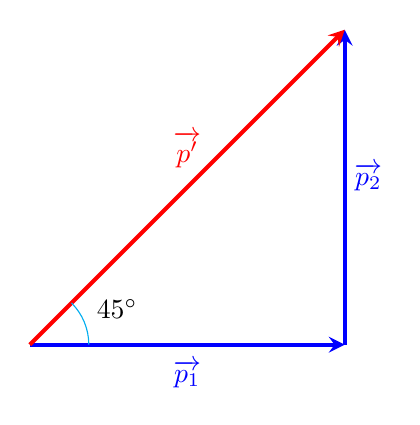
\begin{tikzpicture}
				\coordinate (O) at (0,0);
				\coordinate (A) at (4,0);
				\coordinate (B) at (4,4);
				\draw[-stealth,line width=1.5, blue] (O) -- (A);
				\draw[-stealth,line width=1.5, blue] (A) -- (B);
				\draw[-stealth,line width=1.5, red] (O) -- (B);
				\node[label={[blue,below]90:$\overrightarrow{p_1}$}] at (2,-0.2){};	
				\node[label={[blue,right]90:$\overrightarrow{p_2}$}] at (4,2){};	
				\node[label={[red,above]90:$\overrightarrow{p'}$}] at (2,2){};	
				\tkzMarkAngle[size=0.75cm,color=cyan](A,O,B);
				\tkzLabelAngle[color=black,pos=1.2](A,O,B){$\SI{45}{\degree}$}
			\end{tikzpicture}
		\end{center}
		Động lượng ban đầu của ô tô thứ nhất:
		$$p_1=\dfrac{p_2}{\tan\SI{45}{\degree}}=p_2$$
		$$\Leftrightarrow m_1v_1=m_2v_2\Rightarrow v_1=\dfrac{m_2v_2}{m_1}=\dfrac{\left(\SI{2000}{\kilogram}\right)\cdot\left(\SI{3}{\meter/\second}\right)}{\SI{1000}{\kilogram}}=\SI{6}{\meter/\second}$$
		Tốc độ của hai xe sau va chạm:
		$$p=\sqrt{p^2_1+p^2_2}=p_2\sqrt{2}$$
		$$\Leftrightarrow \left(m_1+m_2\right)v=m_2v_2\sqrt{2}$$
		$$\Rightarrow v=\dfrac{m_2v_2\sqrt{2}}{m_1+m_2}=\dfrac{\left(\SI{2000}{\kilogram}\right)\cdot\left(\SI{3}{\meter/\second}\right)\sqrt{2}}{\SI{3000}{\kilogram}}\approx\SI{2.83}{\meter/\second}.$$}
\end{ex}	
\Closesolutionfile{ans}
\section{Trắc nghiệm đúng/sai}
\setcounter{ex}{0}
\Opensolutionfile{ans}[ans/VN10-Y24-PH-SYL-030P-TF]
% ===================================================================
\begin{ex}\mkstar{2}
	Một viên bi thép khối lượng $m_1=\SI{2}{\kilogram}$ đang chuyển động với tốc độ $v_1=\SI{3}{\meter/\second}$ đến va chạm vào viên bi khác có khối lượng $m_2=\SI{4}{\kilogram}$ đang chuyển động với tốc độ $v_2=\SI{1}{\meter/\second}$ cùng chiều với nó. Sau va chạm, hai viên bi tách rời nhau và viên bi khối lượng $m_1=\SI{2}{\kilogram}$ tiếp tục chuyển động theo hướng ban đầu với tốc độ $v'_1=\SI{2}{\meter/\second}$.
	\choiceTF[t]
	{Va chạm giữa hai viên bi là va chạm mềm}
	{\True Độ lớn động lượng của viên bi có khối lượng $m_1$ trước va chạm là $\SI{6}{\kilogram\cdot\meter/\second}$}
	{\True Động lượng của hệ hai viên bi trước va chạm có độ lớn là $\SI{10}{\kilogram\cdot\meter/\second}$}
	{Sau va chạm, viên bi khối lượng $m_2=\SI{4}{\kilogram}$ chuyển động với tốc độ là $\SI{1.0}{\meter/\second}$}
	\loigiai{}
\end{ex}
% ===================================================================
\begin{ex}\mkstar{3}
	Một vật có khối lượng $m_1=\SI{1}{\kilogram}$ chuyển động với vận tốc $v_1=\SI{3}{\meter/\second}$ đến va chạm với một vật có khối lượng $m_2=\SI{0.5}{\kilogram}$ đang đứng yên. Sau va chạm, hai vật dính vào nhau và chuyển động với cùng vận tốc.
	\choiceTF[t]
	{Do hai vật dính vào nhau nên động lượng của hệ giảm đi}
	{Tổng động năng của hệ trước và sau va chạm bằng nhau}
	{Động lượng của vật $m_1$ trước va chạm có độ lớn bằng $\SI{4.5}{\kilogram\cdot\meter/\second}$}
	{\True Tốc độ của hai vật sau va chạm bằng $\SI{2}{\meter/\second}$}
	\loigiai{
	\begin{itemchoice}
		\itemch Sai. Động lượng của hệ được bảo toàn.
		\itemch Sai. Đây là va chạm mềm nên động năng của hệ không được bảo toàn.
		\itemch Sai. Động lượng của vật $m_1$ trước va chạm $p_1=m_1v_1=\SI{3}{\kilogram\cdot\meter/\second}$.
		\itemch Đúng. Ta có $m_1v_1+m_2v_2=\left(m_1+m_2\right)v\Rightarrow v=\dfrac{m_1v_1+m_2v_2}{m_1+m_2}=\SI{2}{\meter/\second}$.
	\end{itemchoice}
	}
\end{ex}
% ===================================================================
\begin{ex}\mkstar{3}
	Hai xe lăn nhỏ có khối lượng lần lượt $m_1=\SI{300}{\gram}$, $m_2=\SI{200}{\gram}$ chuyển động ngược chiều hướng vào nhau trên một đường thẳng nằm ngang với các tốc độ tương ứng $\SI{0.2}{\meter/\second}$ và $\SI{0.8}{\meter/\second}$. Sau va chạm, hai xe dính vào nhau.
	\choiceTF[t]
	{\True Sau va chạm, hai xe dính vào nhau nên hai xe chuyển động với cùng một vận tốc}
	{Chọn chiều dương là chiều chuyển động của xe $m_1$. Vận tốc của hai xe sau va chạm có giá trị là $\SI{0.2}{\meter/\second}$}
	{\True Động năng của hệ trước va chạm và sau khi va chạm có giá trị lần lượt là $\SI{0.07}{\joule}$ và $\SI{0.01}{\joule}$}
	{Phần năng lượng bị tiêu hao trong quá trình va chạm là $\SI{0.08}{\joule}$}
	\loigiai{
	\begin{itemchoice}
		\itemch Đúng.
		\itemch Sai. Vì các vận tốc cùng phương nên
		\begin{equation}
			\label{eq: 30P.6}
			\left(m_1+m_2\right)v'=m_1v_1+m_2v_2
		\end{equation}
		Chọn chiều dương là chiều chuyển động ban đầu của xe 1, ta có:
		\begin{equation}
			\label{eq: 30P.7}
			\begin{cases}
				v_1=\SI{0.2}{\meter/\second}\\
				v_2=\SI{-0.8}{\meter/\second}
			\end{cases}
		\end{equation}
		Thay \eqref{eq: 30P.7} vào \eqref{eq: 30P.7}, ta có: $v'=\dfrac{m_1v_1+m_2v_2}{m_1+m_2}=\SI{-0.2}{\meter/\second}$.
		\itemch Đúng.\\
		Động năng của hệ trước va chạm $W_{\text{đ}_t}=\dfrac{1}{2}m_1v^2_1+\dfrac{1}{2}m_2v^2_2=\SI{0.07}{\joule}$.\\
		Động năng của hệ sau va chạm $W_{\text{đ}_s}=\dfrac{1}{2}\left(m_1+m_2\right)v'^2=\SI{0.01}{\joule}$.
		\itemch Sai. Phần năng lượng bị tiêu hao trong va chạm: $\Delta W_{\text{đ}}=W_{\text{đ}_t}-W_{\text{đ}_s}=\SI{0.06}{\joule}$.
	\end{itemchoice}
	}
\end{ex}
\Closesolutionfile{ans}
\section{Tự luận}
\setcounter{ex}{0}
\Opensolutionfile{ans}[ans/VN10-Y24-PH-SYL-030P-TL]
% ======================================================================
\begin{ex}\mkstar{2}
	Vật $\SI{200}{\gram}$ chuyển động với tốc độ $\SI{6}{\meter/\second}$ đến va chạm với vật $\SI{50}{\gram}$ chuyển động với tốc độ $\SI{4}{\meter/\second}$. Sau va chạm vật $\SI{200}{\gram}$ giữ nguyên hướng và chuyển động với tốc độ bằng nửa vận tốc ban đầu. Tính tốc độ của vật còn lại trong các trường hợp sau:
	\begin{enumerate}[label=\alph*)]
		\item Trước va chạm hai vật chuyển động cùng chiều.
		\item Trước va chạm hai vật chuyển động ngược chiều.
	\end{enumerate}
	\loigiai{\begin{enumerate}[label=\alph*)]
			\item Trước va chạm hai vật chuyển động cùng chiều.\\
			Áp dụng định luật bảo toàn động lượng cho hai vật ngay trước và sau va chạm:
			\begin{equation}
				\label{eq:30-P.1}
				m_1\vec v_1+m_2\vec v_2=m_1\overrightarrow{v'_1}+m_2\overrightarrow{v'_2}
			\end{equation}
			Chiếu phương trình (\ref{eq:30-P.1}) lên chiều chuyển động ban đầu của vật 1:
			$$m_1v_1 + m_2 v_2 = m_1v_1' + m_2 v_2' $$
			$$\Rightarrow v_2'=\dfrac{m_1v_1+m_2v_2-\dfrac{m_1v_1}{2}}{m_2}=\dfrac{\dfrac{\left(\SI{0.2}{\kilogram}\right)\cdot\left(\SI{6}{\meter/\second}\right)}{2}+\left(\SI{0.05}{\kilogram}\right)\cdot\left(\SI{4}{\meter/\second}\right)}{\SI{0.05}{\kilogram}}=\SI{16}{m/s}.$$
			\item Trước va chạm hai vật chuyển động ngược chiều.
			Áp dụng định luật bảo toàn động lượng cho hai vật ngay trước và sau va chạm:
			\begin{equation}
				\label{eq:30-P.2}
				m_1\vec v_1+m_2\vec v_2=m_1\overrightarrow{v'_1}+m_2\overrightarrow{v'_2}
			\end{equation}
			Chiếu phương trình (\ref{eq:30-P.2}) lên chiều chuyển động ban đầu của vật 1:
			$$m_1v_1 - m_2 v_2 = m_1v_1' + m_2 v_2' $$
			$$\Rightarrow v_2'=\dfrac{m_1v_1-m_2v_2-\dfrac{m_1v_1}{2}}{m_2}=\dfrac{\dfrac{\left(\SI{0.2}{\kilogram}\right)\cdot\left(\SI{6}{\meter/\second}\right)}{2}-\left(\SI{0.05}{\kilogram}\right)\cdot\left(\SI{4}{\meter/\second}\right)}{\SI{0.05}{\kilogram}}=\SI{8}{m/s}.$$
	\end{enumerate}}
\end{ex}
% ======================================================================
\begin{ex}\mkstar{2}
Một vật khối lượng $\SI{0.8}{kg}$ chuyển động trên mặt phẳng ngang với tốc độ $\SI{12}{m/s}$, đến va chạm với một vật khác có khối lượng $\SI{0.2}{kg}$ đang đứng yên trên mặt phẳng ngang ấy. Sau va chạm hai vật nhập lại làm một và chuyển động với cùng tốc độ. Tính tốc độ của hai vật sau va chạm.	
	\loigiai{Áp dụng định luật bảo toàn động lượng cho hai vật ngay trước và sau va chạm:
		\begin{equation}
			\label{eq:30-P.3}
			m_1\vec v_1+m_2\vec v_2=\left(m_1+m_2\right)\vec v
		\end{equation}
		Chiếu phương trình (\ref{eq:30-P.3}) lên chiều chuyển động ban đầu của vật 1:
		$$m_1v_1= (m_1 + m_2) v \Rightarrow v=\dfrac{m_1v_1}{m_1+m_2}=\dfrac{\left(\SI{0.8}{\kilogram}\right)\cdot\left(\SI{12}{\meter/\second}\right)}{\SI{0.8}{\kilogram}+\SI{0.2}{\kilogram}}=\SI{9.6}{m/s}.$$}
\end{ex}
% ======================================================================
\begin{ex}\mkstar{2}
Một vật khối lượng $m_1=\SI{400}{g}$ chuyển động trên mặt phẳng ngang với vận tốc $\SI{18}{km/h}$, đến va chạm với một vật khác có khối lượng $\SI{100}{g}$ đang đứng yên trên mặt phẳng ngang ấy. Sau va chạm hai vật nhập lại làm một và chuyển động với cùng vận tốc. Tính vận tốc của hai vật sau va chạm.	
	\loigiai{Áp dụng định luật bảo toàn động lượng trong va chạm mềm (hai vật dính vào nhau sau va chạm):
		$$m_1v_1 + m_2 v_2 = (m_1 + m_2) v \Rightarrow v=\SI{4}{m/s}.$$}
\end{ex}		
% ======================================================================
\begin{ex}\mkstar{2}
Một khẩu súng $M = \SI{4}{kg}$ bắn ra viên đạn $m = \SI{20}{g}$. Vận tốc của đạn ra khỏi nòng súng là $\SI{600}{m/s}$. Súng giật lùi với vận tốc $V$ có độ lớn là bao nhiêu?	
	\loigiai{
	Chọn chiều dương là chiều chuyển động của viên đạn.\\
	Áp dụng bảo toàn động lượng cho hệ đạn và súng ngay trước và sau khi bắn:
	\begin{equation}
		\label{eq:30-P.4}
		\vec 0=m\vec v+M\vec V
	\end{equation}
	$$\Rightarrow V=-\dfrac{m}{M}\cdot\vec v$$
	Súng bị giật trở lại với tốc độ:
	$$V=\dfrac{mv}{M}=\dfrac{\left(\SI{0.02}{\kilogram}\right)\cdot\left(\SI{600}{\meter/\second}\right)}{\SI{4}{\kilogram}}=\SI{3}{\meter/\second}.$$
	}
\end{ex}
% ======================================================================
\begin{ex}\mkstar{2}
Một tên lửa khối lượng tổng cộng 70 tấn đang bay với tốc độ $\SI{200}{m/s}$ đối với Trái Đất thì tức thời phụt ra lượng khí 5 tấn, với tốc độ $\SI{450}{m/s}$ đối với tên lửa. Xác định vận tốc của tên lửa sau khi phụt khí ra.	
	\loigiai{Gọi:
		\begin{itemize}
			\item (1) khí phụt ra sau tên lửa;
			\item (2) tên lửa;
			\item (0) mặt đất.
		\end{itemize}
		Ta có: $v_{20}=\SI{200}{\meter/\second}$; $v'_{12}=\SI{450}{\meter/\second}$.\\
		Áp dụng định luật bảo toàn động lượng cho hệ tên lửa và khí ngay trước và sau khi khí phụt ra:
		\begin{eqnarray*}
			\left(m_1+m_2\right)\overrightarrow{v_{20}}&=&m_1\overrightarrow{v'_{10}}+m_2\overrightarrow{v'_{20}}\\
			\Leftrightarrow \left(m_1+m_2\right)\overrightarrow{v_{20}}&=&m_1\left(\overrightarrow{v'_{12}}+\overrightarrow{v_{20}}\right)+m_2\overrightarrow{v'_{20}}\\
			\Rightarrow m_2\overrightarrow{v_{20}}&=&m_1\overrightarrow{v'_{12}}+m_2\overrightarrow{v'_{20}} \quad (*)
		\end{eqnarray*}
		Chiếu phương trình (*) lên chiều chuyển động ban đầu của tên lửa, thu được:
		$$m_2v_{20}=-m_1v'_{12}+m_2v'_{20}$$
		$$\Rightarrow v'_{20}=\dfrac{m_2v_{20}+m_1v'_{12}}{m_2}=\dfrac{\left(\SI{65E3}{\kilogram}\right)\cdot\left(\SI{200}{\meter/\second}\right)+\left(\SI{5E3}{\kilogram}\right)\cdot\left(\SI{450}{\meter/\second}\right)}{\SI{65E3}{\kilogram}}\approx\SI{234.6}{\meter/\second}.$$}
\end{ex}
% ======================================================================
\begin{ex}\mkstar{3}
	Một ô tô con khối lượng 1,2 tấn đang chuyển động với tốc độ $\SI{25}{\meter/\second}$ thì va chạm vào đuôi của một xe tải khối lượng 9 tấn đang chạy cùng chiều với tốc độ $\SI{20}{\meter/\second}$ . Sau va chạm, ô tô con vẫn chuyển động theo hướng cũ với tốc độ $\SI{18}{\meter/\second}$.
	\begin{enumerate}[label=\alph*)]
		\item Xác định vận tốc của xe tải ngay sau va chạm.
		\item Xác định phần năng lượng tiêu hao trong quá trình va chạm. Giải thích tại sao có sự tiêu hao năng lượng này.
	\end{enumerate}
	\loigiai{\begin{enumerate}[label=\alph*)]
			\item Gọi:
			\begin{itemize}
				\item $m_1$, $m_2$ lần lượt là khối lượng xe ô tô và xe tải;
				\item $v_1$, $v'_1$, $v_2$, $v'_2$ lần lượt là vận tốc của xe ô tô, xe tải trước và sau va chạm.
			\end{itemize}
			Áp dụng định luật bảo toàn động lượng cho hệ ô tô và xe tải ngay trước và sau va chạm:
			\begin{equation}
				\label{eq:30-P.5}
				m_1\vec v_1+m_2\vec v_2=m_1\overrightarrow{v'_1}+m_2\overrightarrow{v'_2}
			\end{equation}
			Chiếu (\ref{eq:30-P.5}) lên hướng chuyển động ban đầu của ô tô:
			$$m_1v_1+m_2v_2=m_1v'_1+m_2v'_2\Rightarrow v'_2=\dfrac{m_1v_1+m_2v_2-m_1v'_1}{m_2}\approx\SI{20.93}{\meter/\second}.$$
			Như vậy, xe ô tô tải vẫn chuyển động theo hướng cũ với tốc độ $\SI{20.93}{\meter/\second}.$
			\item Năng lượng tiêu hao trong quá trình va chạm:
			$$\Delta W=\dfrac{1}{2}m_1v^2_1+\dfrac{1}{2}m_2v^2_2-\left(\dfrac{1}{2}m_1v'^2_1+\dfrac{1}{2}m_2v'^2_2\right)\approx\SI{9308}{\joule}.$$
			Năng lượng tiêu hao làm biến dạng kết cấu của hai xe, động năng của các mảng vỡ, nhiệt lượng ở bề mặt tiếp xúc.
			
	\end{enumerate}}
\end{ex}
% ======================================================================
\begin{ex}\mkstar{3}
	Con lắc đạn đạo là thiết bị được sử dụng để đo tốc độ của viên đạn. Viên đạn được bắn vào một khúc gỗ lớn treo lơ lửng bằng dây nhẹ, không dãn. Sau khi va chạm, viên đạn ghim vào trong khối gỗ. Sau đó, toàn bộ hệ khối gỗ và viên đạn chuyển động như một con lắc lên độ cao $h$ (xem hình). Xét viên đạn có khối lượng $m_1=\SI{5}{\gram}$, khối gỗ có khối lượng $m_2=\SI{1}{\kilogram}$ và  $h=\SI{5}{\centi\meter}$. Lấy $g=\SI{9.8}{\meter/\second^2}$. Bỏ qua sức cản của không khí
	\begin{center}
		\includegraphics[width=0.35\linewidth]{../figs/VN10-2023-PH-TP030-P-2}
	\end{center}
	\begin{enumerate}[label=\alph*)]
		\item Tính vận tốc của hệ sau khi viên đạn ghim vào khối gỗ.
		\item Tính tốc độ ban đầu của viên đạn.
	\end{enumerate}
	\loigiai{\begin{enumerate}[label=\alph*)]
			\item Chọn gốc thế năng tại vị trí thấp nhất của con lắc.\\
			Áp dụng định luật bảo toàn cơ năng cho hệ ngay sau khi va chạm cho đến khi con lắc đạt độ cao cực đại:
			$$\dfrac{1}{2}\left(m_1+m_2\right)v^2=\left(m_1+m_2\right)gh\Rightarrow v=\sqrt{2gh}\approx\SI{0.99}{\meter/\second}.$$
			\item Áp dụng định luật bảo toàn động lượng cho hệ khối gỗ - viên đạn ngay trước và sau va chạm:
			$$m_1\vec v_0=\left(m_1+m_2\right)\vec v\Rightarrow \vec v_0=\dfrac{\left(m_1+m_2\right)}{m_1}\cdot\vec v$$
			Tốc độ ban đầu của viên đạn:
			$$v_0=\dfrac{\left(m_1+m_2\right)v}{m_1}\approx\SI{198.99}{\meter/\second}.$$
	\end{enumerate}}
\end{ex}
% ======================================================================
\begin{ex}\mkstar{4}
\immini{	Một khẩu pháo được gắn chặt vào xe và xe có thể di chuyển dọc theo đường ray nằm ngang như hình. Khẩu pháo bắn ra một viên đạn khối lượng $\SI{200}{\kilogram}$ với tốc độ $\SI{125}{\meter/\second}$ theo hướng hợp với phương ngang một góc $\SI{45}{\degree}$. Biết khối lượng của khẩu pháo và xe là $\SI{5000}{\kilogram}$. Tính tốc độ giật lùi của khẩu pháo.}
{\includegraphics[scale=0.6]{../figs/VN10-2023-PH-TP030-P-3}}
	\loigiai{Gọi 
		\begin{itemize}
			\item $\vec v_1$, $\vec v_2$ lần lượt là vận tốc của viên đạn và khẩu pháo ngay sau khi bắn;
			\item $m_1$, $m_2$ lần lượt là khối lượng của viên đạn và khẩu pháo.
		\end{itemize}
		Áp dụng định luật bảo toàn động lượng cho hệ viên đạn - khẩu pháo ngay trước và sau khi bắn:
		$$\vec 0=m_1\vec v_1+m_2\vec v_2\Rightarrow \vec v_2=-\dfrac{m_1\vec v_1}{m_2}$$
		Nghĩa là pháo bị giật lùi cùng phương, ngược chiều vector vận tốc của đạn.\\
		Tốc độ giật lùi:
		$$v_2=\dfrac{m_1v_1}{m_2}=\SI{5}{\meter/\second}.$$
		Tốc độ giật lùi của khẩu pháo theo phương ngang:
		$$v_{2x}=v_2\cos\SI{45}{\degree}\approx\SI{3.54}{\meter/\second}.$$}
\end{ex}
\Closesolutionfile{ans}
				\stopMyChapterToc
		\stopPartToc
		\chapter*{Ôn tập chương \thepart}
		\addcontentsline{toc}{mychapter}{\bfseries Ôn tập chương \thepart}
		\let\lesson\undefined
\newcommand{\lesson}{\phantomlesson{Ôn tập chương 7}}
\setcounter{ex}{0}
\Opensolutionfile{ans}[ans/VN10-2023-PH-TP0007-TN]
% ===================================================================
\begin{ex}\mkstar{1}
Đơn vị của động lượng bằng	
	\choice
	{$\si{\newton/\second}$}
	{\True N$\cdot$s}
	{N$\cdot$m}
	{N$\cdot$m/s}
	\loigiai{}
\end{ex}
	
% ===================================================================
\begin{ex}\mkstar{1}
Điều nào sau đây \textbf{sai} khi nói về động lượng?	
	\choice
	{Động lượng của một vật có độ lớn bằng tích khối lượng và tốc độ của vật}
	{Trong hệ kín, động lượng của hệ được bảo toàn}
	{\True Động lượng của một vật có độ lớn bằng tích khối lượng và bình phương vận tốc}
	{Động lượng của một vật là một đại lượng vector}
	\loigiai{}
\end{ex}
% ===================================================================
\begin{ex}\mkstar{1}
Chọn câu phát biểu đúng nhất?	
	\choice
	{Vector động lượng của hệ được bảo toàn}
	{Vector động lượng toàn phần của hệ được bảo toàn}
	{\True Vector động lượng toàn phần của hệ kín được bảo toàn}
	{Động lượng của hệ kín được bảo toàn}
	\loigiai{}
\end{ex}
% ===================================================================
\begin{ex}\mkstar{1}
	Động lượng của vật bảo toàn trong trường hợp nào sau đây? 
	\choice
	{\True Vật đang chuyển động thẳng đều trên mặt phẳng nằm ngang}
	{Vật đang chuyển động tròn đều}
	{Vật đang chuyển động nhanh dần đều trên mặt phẳng nằm ngang không ma sát}
	{Vật đang chuyển động chậm dần đều trên mặt phẳng nằm ngang không ma sát}
	\loigiai{}
\end{ex}
	% ===================================================================
	\begin{ex}\mkstar{1}
		Vector động lượng là vector 
		\choice
		{có phương vuông góc với vector vận tốc}
		{\True cùng phương, cùng chiều với vector vận tốc}
		{cùng phương, ngược chiều với vector vận tốc}
		{có phương hợp với vector vận tốc một góc bất kì}
		\loigiai{}
	\end{ex}
% ===================================================================
\begin{ex}\mkstar{2}
	Biểu thức nào sau đây mô tả đúng mối quan hệ giữa động lượng và động năng?	
		\choice
		{$p=\sqrt{mW_{\text{đ}}}$}
		{$p=mW_{\text{đ}}$}
		{\True $p=\sqrt{2mW_{\text{đ}}}$}
		{$p=2mW_{\text{đ}}$}
		\loigiai{Ta có:
			\begin{align*}
				\begin{cases}
					W_{\text{đ}}=\dfrac{1}{2}mv^2\\
					p=mv
				\end{cases}
				\Rightarrow p^2=2mW_{\text{đ}}\Leftrightarrow p=\sqrt{2mW_{\text{đ}}}
		\end{align*}}
	\end{ex}
% ===================================================================
\begin{ex}\mkstar{1}
Trong trường hợp nào sau đây, hệ có thể xem là hệ kín?	
	\choice
	{Hai viên bi chuyển động trên mặt phẳng nằm ngang}
	{Hai viên bi chuyển động trên mặt phẳng nghiêng}
	{Hai viên bi rơi thẳng đứng trong không khí}
	{\True Hai viên bi chuyển động không ma sát trên mặt phẳng nằm ngang}
	\loigiai{}
\end{ex}
% ===================================================================
\begin{ex}\mkstar{2}
	Trong các quá trình chuyển động sau đây, quá trình nào mà động lượng của vật không thay đổi?
	\choice
	{Vật chuyển động chạm vào vách và phản xạ lại}
	{Vật được ném ngang}
	{Vật đang rơi tự do}
	{\True Vật chuyển động thẳng đều}
	\loigiai{}
\end{ex}
% ===================================================================
\begin{ex}\mkstar{2}
Va chạm đàn hồi và va chạm mềm khác nhau ở điểm nào sau đây?	
	\choice
	{Hệ va chạm đàn hồi có động lượng bảo toàn còn va chạm mềm thì động lượng không bảo toàn}
	{\True Hệ va chạm đàn hồi có động năng không thay đổi còn va chạm mềm thì động năng thay đổi}
	{Hệ va chạm mềm có động năng không thay đổi còn va chạm đàn hồi thì động năng thay đổi}
	{Hệ va chạm mềm có động lượng bảo toàn còn va chạm đàn hồi thì động lượng không bảo toàn}
	\loigiai{}
\end{ex}
% ===================================================================
\begin{ex}\mkstar{2}
	Cho hai vật va chạm trực diện với nhau, sau va chạm, hai vật dính liền thành một khối và chuyển động với cùng vận tốc. Động năng của hệ ngay trước và sau va chạm lần lượt là $W_\text{đ}$ và $W'_\text{đ}$. Biểu thức nào dưới đây là đúng?
	\choice
	{$W_\text{đ}=W_\text{đ'}$}
	{$W_\text{đ}<W'_\text{đ}$}
	{\True $W_\text{đ}>W'_\text{đ}$}
	{$W_\text{đ}=2W'_\text{đ}$}
	\loigiai{Trong hệ va chạm mềm, cơ năng của hệ sau va chạm bé hơn cơ năng của hệ trước va chạm.}
\end{ex}
% ===================================================================
\begin{ex}\mkstar{2}
	Hai vật có khối lượng $m_1$ và $m_2$ chuyển động với vận tốc lần lượt là $\vec v_1$ và $\vec v_2$. Động lượng của hệ có giá trị 
	\choice
	{$m\vec v$}
	{\True $m_1\vec v_1+m_2\vec v_2$}
	{0}
	{$m_1v_1+m_2v_2$}
	\loigiai{}
\end{ex}
% ===================================================================
\begin{ex}\mkstar{2}
Vật 1 khối lượng $m$ đang chuyển động với tốc độ $v_0$ đến va chạm đàn hồi với vật 2 có cùng khối lượng và đang đứng yên. Nếu khối lượng vật 2 tăng lên gấp đôi thì động năng của hệ sau va chạm	
	\choice
	{\True không đổi}
	{tăng 2 lần}
	{giảm 1,5 lần}
	{tăng 1,5 lần}
	\loigiai{Vì va chạm là đàn hồi nên động năng của hệ sau va chạm bằng động năng của hệ trước va chạm và bằng động năng của vật 1 trước va chạm $W_\text{đ}=\dfrac{1}{2}m_1v^2_0$ (ban đầu vật 2 đứng yên).}
\end{ex}
% ===================================================================
\begin{ex}\mkstar{2}
	Một vật chuyển động với tốc độ tăng dần thì có
	\choice
	{động lượng không đổi}
	{động lượng bằng không}
	{\True động lượng tăng dần}
	{động lượng giảm dần}
	\loigiai{}
\end{ex}
% ===================================================================
\begin{ex}\mkstar{2}
	Quả cầu A khối lượng $m_1$ chuyển động với vận tốc $\vec v_1$ va chạm vào quả cầu B khối lượng $m_2$ đứng yên. Sau va chạm, cả hai quả cầu có cùng vận tốc $\vec v_2$. Ta có hệ thức
	\choice
	{\True $m_1\vec v_1 = (m_1 + m_2) \vec v_2$}
	{$m_1\vec v_1 = -m_2 \vec v_2$}
	{$m_1\vec v_1 = m_2 \vec v_2$}
	{$m_1\vec v_1 = \dfrac{1}{2}(m_1 + m_2) \vec v_2$}
	\loigiai{}
\end{ex}
% ===================================================================
\begin{ex}\mkstar{2}
Một vật có khối lượng $\SI{4}{kg}$ rơi tự do không vận tốc đầu trong khoảng thời gian $\SI{2,5}{s}$. Lấy $g = \SI{10}{m/s}^2$. Độ biến thiên động lượng của vật trong khoảng thời gian đó có độ lớn là	
	\choice
	{\True $\SI{100}{kg\cdot m/s}$}
	{$\SI{25}{kg\cdot m/s}$}
	{$\SI{50}{kg\cdot m/s}$}
	{$\SI{200}{kg\cdot m/s}$}
	\loigiai{
	Vận tốc ban đầu của vật: 
	$$v_0 = \SI{0}{m/s}.$$
	Vận tốc của ngay trước khi chạm đất
	$$v =gt = \SI{25}{m/s}.$$
	Độ biến thiên động lượng của vật trong khoảng thời gian:
	$$\Delta p = p_2 - p_1 = mv -mv_0 = \SI{100}{kg \cdot m/s}.$$
	}
\end{ex}
	% ===================================================================
	\begin{ex}\mkstar{2}
		Người ta ném một quả bóng khối lượng $\SI{500}{g}$ cho nó chuyển động với tốc độ $\SI{20}{m/s}$. Xung lượng của lực tác dụng lên quả bóng là
		\choice
		{\True $\SI{10}{N\cdot s}$}
		{$\SI{200}{N\cdot s}$}
		{$\SI{100}{N\cdot s}$}
		{$\SI{20}{N\cdot s}$}
		\loigiai{Xung lượng của lực tác dụng là
			$$F \cdot \Delta t= \Delta p = mv = \SI{10}{N\cdot s}.$$}
	\end{ex}
	% ===================================================================
	\begin{ex}\mkstar{2}
		Hai vật có khối lượng $m_1 = 2m_2$, chuyển động với vận tốc có độ lớn $v_1 = 2v_2$. Động lượng của hai vật có quan hệ
		\choice
		{$p_1 = 2p_2$}
		{\True $p_1 = 4p_2$}
		{$p_2 = 4p_1$}
		{$p_1 = p_2$}
		\loigiai{Ta có:
			$$\dfrac{p_1}{p_2} = \dfrac{m_1v_1}{m_2v_2} = \dfrac{2 \cdot 2 m_2v_2}{m_2v_2} = 4.$$
			Suy ra: $p_1 = 4p_2.$}
	\end{ex}
% ===================================================================
\begin{ex}\mkstar{2}
Một chất điểm chuyển động không vận tốc đầu dưới tác dụng của lực $F = \xsi{10^{-2}}{N}$. Động lượng chất điểm ở thời điểm $t = \SI{3}{s}$ kể từ lúc bắt đầu chuyển động là 	
	\choice
	{$\xsi{2 \cdot 10^{-2}}{kg \cdot m/s}$}
	{\True $\xsi{3 \cdot 10^{-2}}{kg \cdot m/s}$}
	{$\xsi{ 10^{-2}}{kg \cdot m/s}$}
	{$\xsi{6 \cdot 10^{-2}}{kg \cdot m/s}$}
	\loigiai{Ta có:		
		$$p = F\Delta t = \xsi{3\cdot 10^{-2}}{kg\cdot m/s}.$$}
\end{ex}
% ===================================================================
\begin{ex}\mkstar{2}
Một vật nhỏ khối lượng $m =\SI{2}{kg}$ trượt xuống một đường dốc thẳng nhẵn tại một thời điểm xác định có vận tốc $\SI{3}{m/s}$, sau đó $\SI{4}{s}$ có vận tốc $\SI{7}{m/s}$, tiếp ngay sau đó $\SI{3}{s}$ vật có động lượng là 	
	\choice
	{$\SI{6}{kg\cdot m/s}$}
	{$\SI{10}{kg\cdot m/s}$}
	{\True $\SI{20}{kg\cdot m/s}$}
	{$\SI{28}{kg\cdot m/s}$}
	\loigiai{Ta có: $$a = \dfrac{v - v_0}{4} = \SI{1}{m/s}^2.$$
		Vận tốc sau $\SI{3}{s}$ là:
		$$v' = v + at = \SI{10}{m/s}.$$
		Động lượng của vật
		$$ p =mv' = \SI{20}{kg \cdot m/s}.$$}
\end{ex}
% ===================================================================
\begin{ex}\mkstar{2}
Vật $m_1=\SI{1}{\kilogram}$ chuyển động với tốc độ $v_1$ đến va chạm mềm vào vật $m_2 =\SI{2}{\kilogram}$ đang nằm yên. Ngay sau va chạm tốc độ của vật $m_2$ là $v_2 =\SI{2}{\meter/\second}$. Tốc độ của vật $m_1$ trước va chạm là
	\choice
	{\True $v_1=\SI{6}{\meter/\second}$}
	{$v_1=\SI{1.2}{\meter/\second}$}
	{$v_1=\SI{5}{\meter/\second}$}
	{$v_1=\SI{6}{\meter/\second}$}
	\loigiai{Áp dụng định luật bảo toàn động lượng cho hai vật $m_1$, $m_2$ ngay trước và sau va chạm:
		$$m_1\vec v_1=\left(m_1+m_2\right)\vec v_2$$
		$$\Rightarrow\vec v_1=\dfrac{\left(m_1+m_2\right)\vec v_2}{m_1}$$
		$$\Rightarrow v_1=\dfrac{\left(m_1+m_2\right)v_2}{m_1}=\SI{6}{\meter/\second}.$$}
\end{ex}
% ===================================================================
\begin{ex}\mkstar{2}
Hai vật có khối lượng $m_1 =\SI{2}{\kilogram}$ và $m_2 =\SI{5}{\kilogram}$ chuyển động với tốc độ $v_1 =\SI{5}{\meter/\second}$ và $v_2 =\SI{2}{\meter/\second}$. Tổng động lượng của hệ trong các trường hợp $\vec v_1$, và $\vec v_2$ cùng phương, ngược chiều là	
	\choice
	{\True $\SI{0}{\kilogram\cdot\meter\second^{-1}}$}
	{$\SI{3}{\kilogram\cdot\meter\second^{-1}}$}
	{$\SI{6}{\kilogram\cdot\meter\second^{-1}}$}
	{$\SI{10}{\kilogram\cdot\meter\second^{-1}}$}
	\loigiai{Vì $\vec p_1\uparrow\downarrow\vec p_2$ nên tổng động lượng của hệ:
		$$p=\left|p_2-p_1\right|=\SI{0}{\kilogram\cdot\meter\second^{-1}}.$$}
\end{ex}
% ===================================================================
\begin{ex}\mkstar{3}
	Hai xe có khối lượng $m_1$ và $m_2$ chuyển động ngược chiều nhau với tốc độ $v_1 =\SI{10}{\meter/\second}$; $v_2 =\SI{4}{\meter/\second}$. Sau va chạm 2 xe bị bật trở lại với cùng tốc độ $v'_1=v'_2=\SI{5}{\meter/\second}$. Tỉ số khối lượng của xe 1 đối với xe 2 là
	\choice
	{\True 0,6}
	{0,2}
	{$\dfrac{5}{3}$}
	{5}
	\loigiai{Áp dụng định luật bảo toàn động lượng cho hai xe ngay trước và sau va chạm:
		$$m_1\vec v_1+m_2\vec v_2=m_1\overrightarrow{v'}_1+m_2\overrightarrow{v'}_2$$
		Chiếu phương trình bảo toàn động lượng lên chiều chuyển động ban đầu của $m_1$:
		$$m_1v_1-m_2v_2=-m_1v'_1+m_2v'_2$$
		$$\Rightarrow \dfrac{m_1}{m_2}=\dfrac{v_2+v'_2}{v_1+v'_1}=0,6.$$}
\end{ex}
% ===================================================================
\begin{ex}\mkstar{3}
	Cho một vật khối lượng $m_1$ đang chuyển động với với vận tốc $\SI{5}{\meter/\second}$ đến va chạm với vật hai có khối lượng $\SI{1}{\kilogram}$ đang chuyển động với vận tốc $\SI{1}{\meter/\second}$, hai vật chuyển động cùng chiều. Sau va chạm 2 vật dính vào nhau và cùng chuyển động với vận tốc $\SI{2.5}{\meter/\second}$. Xác định khối lượng $m_1$.
	\choice
	{$\SI{1}{\kilogram}$}
	{\True $\SI{0.6}{\kilogram}$}
	{$\SI{2}{\kilogram}$}
	{$\SI{3}{\kilogram}$}
	\loigiai{Áp dụng định luật bảo toàn động lượng cho hệ hai viên bi ngay trước và sau va chạm:
		$$m_1\vec v_1+m_2\vec v_2=\left(m_1+m_2\right)\vec v$$
		Chiếu phương trình bảo toàn động lượng lên chiều chuyển động ban đầu của hai hòn bi:
		$$m_1v_1+m_2v_2=\left(m_1+m_2\right)v$$
		$$\Rightarrow m_1=\dfrac{m_2\left(v-v_2\right)}{v_1-v}=\SI{0.6}{\kilogram}.$$}
\end{ex}
% ===================================================================
\begin{ex}\mkstar{3}
	Cho viên bi thứ nhất có khối lượng $\SI{200}{\gram}$ đang chuyển động trên mặt phẳng nằm ngang với vận tốc $\SI{5}{\meter/\second}$ tới va chạm vào viên bi thứ hai có khối lượng $\SI{400}{\gram}$ đang đứng yên, biết rằng sau va chạm viên bi thứ hai chuyển động với vận tốc $\SI{3}{\meter/\second}$, chuyển động của hai bi trên cùng một đường thẳng. Xác định độ lớn vận tốc của viên bi thứ nhất sau va chạm.
	\choice
	{$\SI{4}{\meter/\second}$}
	{\True $\SI{1}{\meter/\second}$}
	{$\SI{6}{\meter/\second}$}
	{$\SI{5}{\meter/\second}$}
	\loigiai{Chọn chiều dương là chiều chuyển động của bi thứ nhất trước lúc va chạm.\\
		Áp dụng định luật bảo toàn động lượng cho hai viên bi ngay trước và sau va chạm:
		$$m_1\vec v_1+m_2\vec v_2=m_1\overrightarrow{v'_1}+m_2\overrightarrow{v'_2}$$
		Chiếu phương trình bảo toàn động lượng lên chiều dương:
		$$m_1v_1=m_1v'_1+m_2v'_2$$
		$$\Rightarrow v'_1=\dfrac{m_1v_1-m_2v'_2}{m_1}=\dfrac{\left(\SI{0.2}{\kilogram}\right)\cdot\left(\SI{5}{\meter/\second}\right)-\left(\SI{0.4}{\kilogram}\right)\cdot\left(\SI{3}{\meter/\second}\right)}{\SI{0.2}{\kilogram}}=\SI{-1}{\meter/\second}.$$
		Vậy sau va chạm bi thứ nhất chuyển động với tốc độ $\SI{1}{\meter/\second}$ và chuyển động ngược chiều dương đã chọn.}
\end{ex}
% ===================================================================
\begin{ex}\mkstar{3}
	Hai vật nhỏ có khối lượng khác nhau ban đầu ở trạng thái nghỉ. Sau đó, hai vật đồng thời chịu tác dụng của ngoại lực không đổi có độ lớn như nhau và bắt đầu chuyển động. Sau cùng một khoảng thời gian, điều nào sau đây là đúng?
	\choice
	{Động năng của hai vật như nhau}
	{Vật có khối lượng lớn hơn có động năng lớn hơn}
	{\True Vật có khối lượng lớn hơn có động năng nhỏ hơn}
	{Không đủ dữ kiện để so sánh}
	\loigiai{Ta có: $\Delta \vec p=\vec F\cdot\Delta t$.\\
		Ban đầu, vật ở trạng thái nghỉ nên:
		$$\vec p=\vec F\Delta t\Rightarrow p^2=F^2\left(\Delta t\right)^2\Rightarrow2mW_\text{đ}=F^2\left(\Delta t\right)^2 \Rightarrow W_\text{đ}=\dfrac{F^2\left(\Delta t\right)^2}{2m}$$
		Như vậy, vật có khối lượng càng lớn thì động năng càng bé.}
\end{ex}
% ===================================================================
\begin{ex}\mkstar{3}
Một xe ô tô có khối lượng $m_1 = 6\ \text{tấn}$ chuyển động thẳng với vận tốc $v_1=3\ \text{m/s}$, đến tông và dính vào một xe gắn máy đang đứng yên có khối lượng $m_2 = 200\ \text{kg}$. Tính vận tốc của các xe sau va chạm.	
	\choice
	{$\SI{1.9}{\meter/s}$}
	{$\SI{3.9}{\meter/s}$}
	{$\SI{4.9}{\meter/s}$}
	{\True $\SI{2.9}{\meter/s}$}
	\loigiai{Xem hệ hai xe là hệ cô lập, áp dụng định luật bảo toàn động lượng của hệ: 
		$$m_1 \cdot \vec{v_1} = (m_1+m_2)\cdot \vec{v}.$$
		Vì hai xe va chạm mềm nên sẽ chuyển động theo chiều cũ. Tốc độ của hai xe sau va chạm:
		$$v=\frac{m_1 \cdot v_1}{m_1+m_2}= \SI{2.9}{\meter/s}.$$}
\end{ex}
% ===================================================================
\begin{ex}\mkstar{3}
Viên đạn khối lượng $\SI{20}{\gram}$ đang bay với tốc độ $\SI{600}{\meter/\second}$ thì gặp một cánh cửa thép. Đạn xuyên qua cửa trong thời gian $\SI{0.002}{\second}$. Sau khi xuyên qua cánh cửa thì tốc độ của đạn còn $\SI{300}{\meter/\second}$. Lực cản trung bình của cửa tác dụng lên đạn có độ lớn bằng	
	\choice
	{\True $\SI{3000}{\newton}$}
	{$\SI{900}{\newton}$}
	{$\SI{9000}{\newton}$}
	{$\SI{30000}{\newton}$}
	\loigiai{Lực cản trung bình của cửa tác dụng lên đạn:
		$$F=\dfrac{\left|\Delta p\right|}{\Delta t}=\dfrac{m\left(v_1-v_2\right)}{\Delta t}=\SI{3000}{\newton}.$$}
\end{ex}
% ===================================================================
\begin{ex}\mkstar{4}
Một người có khối lượng $m_1=\SI{50}{kg}$ nhảy từ một chiếc xe có khối lượng $m_2 = \SI{80}{kg}$ đang chuyển động theo phương ngang với vận tốc $v = \SI{3}{m/s}$. Biết vận tốc nhảy của người đối với xe lúc chưa thay đổi vận tốc là $v_0 = \SI{4}{m/s}$. Vận tốc của xe sau khi người ấy nhảy ngược chiều đối với xe là	
	\choice
	{\True $\SI{5,5}{m/s}$}
	{$\SI{4,5}{m/s}$}
	{$\SI{0,5}{m/s}$}
	{$\SI{1}{m/s}$}
	\loigiai{Gọi:
		\begin{itemize}
			\item (1) người;
			\item (2) xe;
			\item (0) đất.
		\end{itemize}
		Ta có: $v_{20}=\SI{3}{\meter/\second}$, $v'_{12}=\SI{4}{\meter/\second}$.\\
		Áp dụng định luật bảo toàn động lượng cho hệ người và xe ngay trước và sau khi người nhảy:
		\begin{eqnarray*}
			\left(m_1+m_2\right)\overrightarrow{v_{20}}&=&m_1\overrightarrow{v'_{10}} +m_2\overrightarrow{v'_{20}}\\
			\Leftrightarrow \left(m_1+m_2\right)\overrightarrow{v_{20}}&=&m_1\left(\overrightarrow{v'_{12}}+\overrightarrow{v_{20}}\right) +m_2\overrightarrow{v'_{20}}\\
			\Rightarrow m_2\overrightarrow{v_{20}}&=&m_1\overrightarrow{v'_{12}}+m_2\overrightarrow{v'_{20}} \quad (*)
		\end{eqnarray*}		
		Chiếu phương trình (*) lên chiều chuyển động ban đầu của xe:
		$$m_2v_{20}=-m_1v'_{12}+m_2v'_{20}\Rightarrow v'_{20}=\dfrac{m_2v_{20}+m_1v'_{12}}{m2}$$
		$$\Leftrightarrow v'_{20}=\dfrac{\left(\SI{80}{\kilogram}\right)\cdot\left(\SI{3}{\meter/\second}\right)+\left(\SI{50}{\kilogram}\right)\cdot\left(\SI{4}{\meter/\second}\right)}{\SI{80}{\kilogram}}=\SI{5.5}{\meter/\second}$$}
\end{ex}
% ===================================================================
\begin{ex}\mkstar{4}
Tên lửa khối lượng $\SI{500}{kg}$ đang chuyển động với vận tốc  $\SI{200}{m/s}$ thì tách ra làm hai phần. Phần bị tháo rời có khối lượng $\SI{200}{kg}$ sau đó chuyển động ra phía sau với vận tốc $\SI{100}{m/s}$ so với phần còn lại. Vận tốc phần còn lại bằng	
	\choice
	{\True $\SI{240}{m/s}$}
	{$\SI{266,7}{m/s}$}
	{$\SI{220}{m/s}$}
	{$\SI{400}{m/s}$}
	\loigiai{Gọi:
		\begin{itemize}
			\item (1) phần tên lửa bị tháo rời;
			\item (2) phần tên lửa còn lại;
			\item (0) mặt đất.
		\end{itemize}
		Áp dụng định luật bảo toàn động lượng cho tên lửa ngay trước và sau khi tách ra:
		\begin{equation}
			\label{eq:30-P.6}
			M\vec V=m_1\vec v_{10}+m_2\vec v_{20}=m_1\left(\vec v_{12}+\vec v_{20}\right)+m_2\vec v_{20}
		\end{equation}
		Chiếu (\ref{eq:30-P.6}) lên chiều chuyển động ban đầu của tên lửa:
		$$MV = m_1\left(v_{20}-v_{12}\right)+m_2v_{20}\Rightarrow v_{20} = \SI{240}{m/s}.$$}
\end{ex}
% ===================================================================
\begin{ex}\mkstar{4}
Một khẩu pháo có khối lượng $m_1 =\SI{130}{\kilogram}$ được đặt trên một toa xe nằm trên đường ray biết toa xe có khối lượng $m_2 =\SI{20}{\kilogram}$ khi chưa nạp đạn. Viên đạn được bắn ra theo phương nằm ngang dọc theo đường ray biết viên đạn có khối lượng $m_3 =\SI{1}{\kilogram}$. Vận tốc của đạn khi bắn ra khỏi nòng súng thì có vận tốc $v_0 = \SI{400}{\meter/\second}$ so với súng. Hãy xác định vận tốc của toa xe sau khi bắn. Biết rằng ban đầu toa xe đang chuyển động với vận tốc $v_1 =\SI{18}{\kilo\meter/\hour}$ theo chiều bắn đạn.	
	\choice
	{$\SI{3.67}{\meter/\second}$}
	{$\SI{5.25}{\meter/\second}$}
	{$\SI{8.76}{\meter/\second}$}
	{\True $\SI{2.33}{\meter/\second}$}
	\loigiai{Áp dụng định luật bảo toàn động lượng cho hệ (xe-khẩu pháo-đạn) ngay trước và sau khi bắn:
		$$\left(m_1+m_2+m_3\right)\overrightarrow{v}_\text{xe/đất}=\left(m_1+m_2\right)\overrightarrow{v'}_\text{xe/đất}+m_3\overrightarrow{v}_\text{đạn/đất}$$
		$$\Leftrightarrow \left(m_1+m_2+m_3\right)\overrightarrow{v}_\text{xe/đất}=\left(m_1+m_2\right)\overrightarrow{v'}_\text{xe/đất}+m_3\left(\overrightarrow{v}_\text{đạn/xe}+\overrightarrow{v}_\text{xe/đất}\right)$$
		Chiếu phương trình bảo toàn động lượng lên chiều chuyển động ban đầu của xe:
		$$\Leftrightarrow \left(m_1+m_2+m_3\right)v_\text{xe/đất}=\left(m_1+m_2\right)v'_\text{xe/đất}+m_3\left(v_\text{đạn/xe}+v_\text{xe/đất}\right)$$
		\begin{eqnarray*}
			\Rightarrow v'_\text{xe/đất}&=&\dfrac{\left(m_1+m_2+m_3\right)v_\text{xe/đất}-m_3\left(v_\text{đạn/xe}+v_\text{xe/đất}\right)}{m_1+m_2}\\
			&=&\dfrac{\left(\SI{130}{\kilogram}+\SI{20}{\kilogram}+\SI{1}{\kilogram}\right)\cdot\left(\SI{5}{\meter/\second}\right)-\left(\SI{1}{\kilogram}\right)\cdot\left(\SI{400}{\meter/\second}+\SI{5}{\meter/\second}\right)}{\SI{130}{\kilogram}+\SI{20}{\kilogram}}\approx\SI{2.33}{\meter/\second}
	\end{eqnarray*}}
\end{ex}

\Closesolutionfile{ans}
		
	\part{CHUYỂN ĐỘNG TRÒN}
		\startPartToc
		\setcounter{mychapter}{20}
			\mychapter[Động học của chuyển động tròn]{Động học của chuyển động tròn}
				\startMyChapterToc
					\let\lesson\undefined
\newcommand{\lesson}{\phantomlesson{Bài 20: Động học của chuyển động tròn.}}
\chapter[Động học của chuyển động tròn]{Động học của chuyển động tròn}
\setcounter{section}{0}
\section{Lý thuyết}
\subsection{Chuyển động tròn}
Chuyển động tròn là chuyển động có quỹ đạo là một đường tròn.\\
\textbf{\textit{Ví dụ:}} một điểm trên cánh quạt chuyển động theo một đường tròn khi cánh quạt quay, chuyển động của một vệ tinh nhân tạo xung quanh Trái Đất.
\begin{center}
	\includegraphics[scale=0.3]{../figs/VN10-PH-06-L-005-1-V2-01.jpg}
\end{center}
\subsection{Tốc độ trung bình trong chuyển động tròn}
 Tốc độ trung bình trong chuyển động tròn là độ dài cung tròn mà vật đi được trong một đơn vị thời gian.
\begin{center}
	\includegraphics[scale=0.3]{../figs/VN10-PH-06-L-005-1-V2-02.jpg}
\end{center}
\subsection{Chuyển động tròn đều}
Chuyển động tròn đều là chuyển động có quỹ đạo tròn và có tốc độ trung bình không đổi trên mọi cung tròn của quỹ đạo. 
\begin{center}
	\includegraphics[scale=0.3]{../figs/VN10-PH-06-L-005-1-V2-03.jpg}
\end{center}
\subsection{Độ dịch chuyển góc}
Giả sử một vật chuyển động trên một đường tròn bán kính $r$. Trong thời gian $\Delta t$ vật đi được quãng đường $\Delta s$. Góc $\Delta \alpha$ ứng với cung tròn $\Delta s$ mà vật đã đi được kể từ vị trí ban đầu gọi là độ dịch chuyển góc:
$$\Delta \alpha = \dfrac{\Delta s}{r}$$
Đơn vị của độ dịch chuyển góc là rad.
\luuy{Trong Vật lí người ta thường đo góc theo đơn vị radian (kí hiệu rad), với $\SI{1}{rad}$ là số đo góc ở tâm một đường tròn chắn cung có độ dài bằng bán kính đường tròn đó.
	$$\SI{1}{rad} = \dfrac{180^\circ}{\pi} = \dfrac{180^\circ}{\SI{3.1416}{}\ldots} \approx\SI{57.2958}{^\circ}$$
	\begin{center}
		\includegraphics{../figs/G10-026-1}
	\end{center}
}
\subsection{Tốc độ góc và tốc độ dài trong chuyển động tròn}
\subsubsection{Tốc độ góc}
Tốc độ góc trong chuyển động tròn có giá trị bằng độ dịch chuyển góc trong một đơn vị thời gian:
$$\omega = \frac{\Delta \alpha}{\Delta t}$$
Đơn vị của tốc độ góc trong hệ đơn vị SI là $\SI{}{\radian/\second}$.\\
Trong chuyển động tròn đều, tốc độ góc của vật không đổi. 
\begin{center}
	\includegraphics[scale=0.3]{../figs/VN10-PH-06-L-005-2-V2-02.jpg}
\end{center}
\subsubsection{Tốc độ dài}
Tốc độ dài (gọi tắt là là tốc độ) của một chất điểm chuyển động tròn được tính bằng quãng đường mà chất điểm di chuyển được trong một đơn vị thời gian:
$$v=\frac{\Delta s}{\Delta t} $$
Đơn vị của tốc độ dài trong hệ đơn vị SI là $\SI{}{\meter/\second.}$.\\
Trong chuyển động tròn đều, tốc độ dài của vật không đổi. \\
\begin{center}
	\includegraphics[scale=0.3]{../figs/VN10-PH-06-L-005-2-V2-01.jpg}
\end{center}	
\begin{minipage}{0.6\textwidth}
	Khi nói về phương, chiều của tốc độ dài, người ta sử dụng khái niệm vector vận tốc (gọi tắt là vận tốc). Vận tốc trong chuyển động tròn có phương tiếp tuyến với đường tròn quỹ đạo và có chiều là chiều của chuyển động.\\
	Trong chuyển động tròn đều, độ lớn của vận tốc tức thời không đổi nhưng hướng luôn thay đổi.
\end{minipage}
\begin{minipage}{0.4\textwidth}
	\begin{center}
		\includegraphics[scale=0.6]{../figs/G10-026-2}
	\end{center}
\end{minipage}
\subsubsection{Liên hệ giữa tốc độ góc và tốc độ dài}
Công thức liên hệ giữa tốc độ góc và tốc độ dài:
$$v=r\omega$$ 
trong đó, $r$ là bán kính quỹ đạo tròn.		
\subsection{Chu kì và tần số}
Ngoài tốc độ, tốc độ góc, trong chuyển động tròn đều người ta còn quan tâm đến các đại lượng như chu kì và tần số.
\subsubsection{Chu kì}
Chu kì (kí hiệu là $T$) trong chuyển động tròn đều là thời gian để vật đi được một vòng tròn.\\
Đơn vị của chu kì trong hệ đơn vị SI là giây $\left(\si{\second}\right)$.
\subsubsection{Tần số}
Tần số (kí hiệu là $f$) là số vòng vật đi được trong một giây.\\
Đơn vị tần số là hertz (Hz).
\subsubsection{Liên hệ giữa chu kì, tần số, và tốc độ góc}
Công thức liên hệ giữa chu kì, tần số và tần số góc:
$$T=\dfrac{1}{f}=\dfrac{2\pi}{\omega},$$
trong đó, $T$ là chu kì, $f$ là tần số, $\omega$ là tốc độ góc. 				
\subsection{Gia tốc hướng tâm}
\begin{center}
	\includegraphics[scale=1]{../figs/G10-027-1}
	\includegraphics[height=5cm]{../figs/G10-027-1b}
\end{center}
\begin{itemize}
	\item Trong chuyển động tròn đều, vector gia tốc $\vec{a}=\frac{\Delta\vec{v}}{\Delta t}$  hướng vào  tâm đường tròn.
	\item vector gia tốc hướng tâm đặc trưng cho sự biến đổi của vector vận tốc, kí hiệu là $\vec{a}_{ht}$.
	\item Độ lớn của vector gia tốc hướng tâm:
	\begin{equation*}
		a_\text{ht}=\frac{v^2}{r}=\omega^2 \cdot r.
	\end{equation*}
	trong đó:
	\begin{itemize}
		\item $a_{\text{ht}}$: độ lớn gia tốc hướng tâm, đơn vị trong hệ SI là $\si{\meter/\second^2}$;
		\item $v$: tốc độ dài, đơn vị trong hệ SI là $\si{\meter/\second}$;
		\item $\omega$: tốc độ góc, đơn vị trong hệ SI là $\si{\radian/\second}$;
		\item $r$: bán kính quĩ đạo, đơn vị trong hệ SI là $\si{\meter}$.
	\end{itemize}
\end{itemize}
\section{Mục tiêu bài học - Ví dụ minh họa}
\begin{dang}{Nhận biết đặc điểm của  chuyển động tròn đều}
	\viduii{1}{Chuyển động nào dưới đây là chuyển động tròn đều?
		\begin{mcq}
			\item Chuyển động của mắt xích xe đạp khi xe chạy.
			\item Chuyển động của đầu cánh quạt trần khi quay ổn định.
			\item Chuyển động của đầu cánh quạt trần khi vừa bật.
			\item Chuyển động của con lắc đồng hồ.
		\end{mcq}
	}
	{\hide{Chuyển động tròn đều là chuyển động có các đặc điểm:
			\begin{itemize}
				\item Quỹ đạo là một đường tròn;
				\item Tốc độ trung bình trên mọi cung tròn là như nhau.
			\end{itemize}
			Chuyển động A không thỏa điều kiện quỹ đạo tròn. Chuyển động C, khi vừa bật quạt thì tốc độ quay của đầu cánh quạt tăng dần. Chuyển động D không thỏa điều kiện tốc độ trung bình như nhau trên mọi cung tròn. Chuyển động B thỏa mãn cả hai điều kiện. \\		
			\textbf{Đáp án: B}.}
	}
	\viduii{1}
	{Chuyển động nào sau đây có thể xem như là chuyển động tròn đều?
	\begin{mcq}
		\item Chuyển động của một vật được ném xiên từ mặt đất.
		\item Chuyển động trong mặt phẳng thẳng đứng của một vật được buộc vào một dây có chiều dài cố định.
		\item Chuyển động của một vệ tinh nhân tạo có vị trí tương đối không đổi với một điểm trên mặt đất (vệ tinh địa tĩnh).
		\item Chuyển động của một quả táo khi rời ra khỏi cành cây.
	\end{mcq}
}
{\hide{Chuyển động tròn đều cần thoả 2 điều kiện:
		\begin{itemize}
			\item Quỹ đạo chuyển động là đường tròn.
			\item Tốc độ trung bình như nhau trên mọi cung tròn.
		\end{itemize}
		Chuyển động của một vật được ném xiên từ mặt đất có quỹ đạo là parabol.\\
		Chuyển động trong mặt phẳng thẳng đứng của một vật được buộc vào một dây có chiều dài cố định chưa hẳn là chuyển động tròn đều vì chưa mô tả rõ trạng thái chuyển động của vật.\\
		Chuyển động của một quả táo khi rời ra khỏi cành cây là chuyển động thẳng biến đổi.\\
		Chuyển động của một vệ tinh nhân tạo có vị trí tương đối không đổi đối với một điểm trên mặt đất (vệ tinh địa tĩnh) là chuyển động tròn đều.\\
		\textbf{Đáp án C.}}
}
	
\end{dang}
\begin{dang}{Biểu diễn đơn vị độ dịch chuyển góc}
	\viduii{2}{Đổi các góc sau từ độ sang radian: $30^\circ$, $90^\circ$.
	}
	{\hide{Ta có:
			$$x^\circ \longrightarrow \dfrac{x \pi}{180}\ \text{rad}.$$
			Đổi $$30^\circ \longrightarrow \dfrac{30\pi}{180}\ \text{rad} = \dfrac{\pi}{6}\ \text{rad}$$
			Đổi $$90^\circ \longrightarrow \dfrac{\SI{90}{\degree}\pi}{\SI{180}{\degree}}\ \text{rad} = \dfrac{\pi}{2}\ \text{rad}.$$}
	}
	\viduii{2}{Đổi các góc sau từ radian sang độ: $\SI{0.25}{rad}$, $\SI{0.5}{rad}$.
	}
	{\hide{Ta có:
			$$x\ \text{rad} \longrightarrow \left(\dfrac{x \cdot 180}{\pi}\right)^\circ.$$
			Đổi $$\SI{0.25}{rad} \longrightarrow \dfrac{0,25 \cdot \SI{180}{\degree}}{\pi} = 14,33^\circ$$
			Đổi $$\SI{0.5}{rad} \longrightarrow \dfrac{0,5 \cdot \SI{180}{\degree}}{\pi} = 28,66^\circ.$$}
	}
\end{dang}
\begin{dang}{Tính tốc độ dài, tốc độ góc, chu kỳ, tần số trong chuyển động tròn đều}
	\viduii{2}{Một vệ tinh nhân tạo bay quanh Trái Đất theo một quỹ đạo tròn. Chu kì của vệ tinh là $88\ \text{phút}$. Tính tốc độ góc của vệ tinh. 
	}
	{\hide{Tốc độ góc của vệ tinh:
			$$T=\frac{2\pi}{\omega} \quad\Rightarrow\quad \omega = \frac{\pi}{2640}\ \text{rad/s}.$$ }
	}
	
	\viduii{3}{
		Kim phút của đồng hồ dài gấp 1,5 lần kim giờ. Hỏi tốc độ dài của đầu kim phút lớn gấp mấy lần tốc độ dài của đầu kim giờ?
	}
	{\hide{Gọi: 
			\begin{itemize}
				\item  $R_1$, $R_2$ lần lượt là chiều dài kim phút và kim giờ
				$$\dfrac{R_1}{R_2}=1,5;$$
				\item $\omega_1, \omega_2$ lần lượt là tốc độ góc của kim phút và kim giờ. Kim phút quay một vòng ($2\pi\ \SI{}{\radian}$) trong 1 giờ, kim giờ quay một vòng trong 12 giờ, do đó 
				$$
				\dfrac{\omega_1}{\omega_2}=12
				$$
			\end{itemize}		
			Ta lập được tỉ số: $$\dfrac{v_1}{v_2}=\dfrac{\omega_1 \cdot R_1}{\omega_2 \cdot R_2}=\dfrac{\omega_1}{\omega_2}\cdot\dfrac{R_1}{R_2}=18.$$}
	}
	
	
	
\end{dang}
\begin{dang}{Tính gia tốc hướng tâm trong chuyển động tròn đều}
	
	\viduii{2}{Một vệ tinh nhân tạo ở độ cao $250\ \text{km}$ bay quanh Trái Đất theo một quỹ đạo tròn. Chu kì của vệ tinh là $88\ \text{phút}$. Tính gia tốc hướng tâm của vệ tinh. Cho bán kính Trái Đất là $6400\ \text{km}$.
	}
	{\hide{Khoảng cách từ vệ tinh đến tâm Trái Đất: 
			$$r=250\ \text{km}+6400\ \text{km} =6650\ \text{km}=6650000\ \text{m}. $$
			Tốc độ góc của vệ tinh:
			$$T=\frac{2\pi}{\omega} \Rightarrow \omega = \frac{\pi}{2640}\ \text{rad/s}.$$ 
			Gia tốc hướng tâm của vệ tinh: 
			$$a_{ht}=\omega^2 \cdot r \approx \SI{9,41}{ \meter/\second^2}.$$ 
		}
	}
	
	\viduii{2}{Một vật chuyển động theo đường tròn bán kính $r = \SI{100}{cm}$ với gia tốc hướng tâm $a_\text{ht} = \SI{4}{cm/s}^2$. Tính chu kì của chuyển động.	
	}
	{\hide{Tốc độ dài của chuyển động
			$$a_\text{ht} =\dfrac{v^2}{r} \Rightarrow v =\sqrt {ra_\text{ht}}.$$
			Chu kì của chuyển động là
			$$T =\dfrac{2\pi}{\omega} = \dfrac{2\pi r}{v} = 2\pi \sqrt{\dfrac{r}{a_\text{ht}}} \approx \SI{31.415}{\second}.$$
		}
	}
\end{dang}
					\let\lesson\undefined
\newcommand{\lesson}{\phantomlesson{Bài 20.}}
\setcounter{section}{2}
\section{Trắc nghiệm nhiều phương án lựa chọn}
\setcounter{ex}{0}
\Opensolutionfile{ans}[ans/VN10-Y24-PH-SYL-031P-TN]
% ===================================================================
\begin{ex}\mkstar{1}
	Biểu thức nào sau đây thể hiện mối liên hệ giữa tốc độ dài, tốc độ góc và chu kì quay?
	\choice
	{$v=\omega R=2\pi TR$}
	{$v=\dfrac{\omega}{R}=\dfrac{2\pi}{T}R$}
	{\True $v=\omega R=\dfrac{2\pi}{T}R$}
	{$v=\dfrac{\omega}{R}=\dfrac{2\pi}{TR}$}
	\loigiai{}
\end{ex}
% ===================================================================
\begin{ex}\mkstar{2}
Chuyển động của vật nào dưới đây được coi là chuyển động tròn đều?	
	\choice
	{Chuyển động của bánh xe ô tô khi đang hãm phanh}
	{\True Chuyển động của kim phút trên mặt đồng hồ chạy đúng giờ}
	{Chuyển động quay của các điểm treo các ghế ngồi trên chiếc đu quay}
	{Chuyển động quay của cánh quạt khi vừa tắt điện}
	\loigiai{Chuyển động của kim phút trên mặt đồng hồ chạy đúng giờ là chuyển động tròn đều.}
\end{ex}
% ===================================================================
\begin{ex}\mkstar{2}
	Các công thức liên hệ giữa tốc độ góc $\omega$ với chu kỳ $T$ và giữa tốc độ góc $\omega$ với tần số $f$ trong chuyển động tròn đều là gì?
	\choice
	{$\omega=2\pi T$; $\omega=\dfrac{2\pi}{f}$}
	{\True $\omega=\dfrac{2\pi}{T}$; $\omega=2\pi f$}
	{$\omega=2\pi T$; $\omega=2\pi f$}
	{$\omega=\dfrac{2\pi}{T}$; $\omega=\dfrac{2\pi}{f}$}
	\loigiai{Công thức liên hệ giữa tốc độ góc $\omega$ với chu kỳ $T$ là $\omega=\dfrac{2\pi}{T}$.
		Công thức liên hệ giữa giữa tốc độ góc $\omega$ với tần số $f$ trong chuyển động tròn đều là $\omega=2\pi f$.}
\end{ex}
% ===================================================================
\begin{ex}\mkstar{2}
Một bánh xe có đường kính $\SI{100}{\centi\meter}$ lăn đều với vận tốc $\SI{36}{\kilo\meter/\hour}$. Gia tốc hướng tâm của một điểm trên vành bánh xe có độ lớn	
	\choice
	{$\SI{200}{\meter/\second^2}$}
	{$\SI{400}{\meter/\second^2}$}
	{\True $\SI{100}{\meter/\second^2}$}
	{$\SI{300}{\meter/\second^2}$}
	\loigiai{Đổi đơn vị: $\SI{100}{\centi\meter}=\SI{1}{\meter}$; $\SI{36}{\kilo\meter/\hour}=\SI{10}{\meter/\second}$\\		
		Gia tốc hướng tâm của một điểm trên vành bánh xe có độ lớn:
		$$a_\text{ht}=\dfrac{v^2}{R}=\SI{100}{\meter/\second^2}.$$}
\end{ex}
% ===================================================================
\begin{ex}\mkstar{2}
	Một đĩa tròn bán kính $\SI{20}{\centi\meter}$ quay đều quanh trục của nó. Đĩa quay hết 1 vòng mất $\SI{0.2}{\second}$. Tốc độ dài $v$ của một điểm nằm ở mép đĩa bằng
	\choice
	{$\SI{4,71}{\meter/\second}$}
	{$\SI{3,14}{\meter/\second}$}
	{\True $\SI{6,28}{\meter/\second}$}
	{$\SI{7,85}{\meter/\second}$}
	\loigiai{Tốc độ dài $v$ của một điểm trên vành ngoài xe:
		$v=r\omega=r\dfrac{\Delta \alpha}{\Delta t}=\SI{0,2}{\meter}\dfrac{2\pi}{\SI{0.2}{\second}}=\SI{6,28}{\meter/\second}$}
\end{ex}
% ===================================================================
\begin{ex}\mkstar{2}
	Một động cơ xe máy có trục quay 1200 vòng/phút. Tốc độ góc của chuyển động quay là bao nhiêu?	
	\choice
	{\True $\SI{125,7}{\radian/\second}$}
	{$\SI{188,5}{\radian/\second}$}
	{$\SI{62,8}{\radian/\second}$}
	{$\SI{7200}{\radian/\second}$}
	\loigiai{Tốc độ góc của chuyển động quay là:
		$\omega$ = 1200 vòng/ phút = $1200\cdot\dfrac{2\pi}{60}\,\SI{}{\radian/\second}=\SI{125,7}{\radian/\second}$}
\end{ex}
% ===================================================================
\begin{ex}\mkstar{2}
Một bánh xe có bán kính $\SI{100}{\centi\meter}$ lăn đều với vận tốc $\SI{54}{\kilo\meter/\hour}$. Gia tốc hướng tâm của một điểm trên vành bánh xe có độ lớn	
	\choice
	{\True $\SI{225}{\meter/\second^2}$}
	{$\SI{400}{\meter/\second^2}$}
	{$\SI{100}{\meter/\second^2}$}
	{$\SI{300}{\meter/\second^2}$}
	\loigiai{Gia tốc hướng tâm của một điểm trên vành bánh xe có độ lớn:
		$$a_\text{ht}=\dfrac{v^2}{R}=\SI{225}{\meter/\second^2}.$$}
\end{ex}
% ===================================================================
\begin{ex}\mkstar{2}
	Xe đạp của một vận động viên chuyển động thẳng đều với $v=\SI{36}{km/h}$. Biết bán kính của lốp xe đạp là $\SI{32.5}{cm}$. Tính tốc độ góc và gia tốc hướng tâm tại một điểm trên lốp bánh xe.
	\choice
	{\True $\omega = \SI{30.77}{rad/s}$, $a_\text{ht} = \SI{307.7}{m/s^2}$}
	{$\omega = \SI{30.77}{rad/s}$, $a_\text{ht} = \SI{377.7}{m/s^2}$}
	{$\omega = \SI{3.77}{rad/s}$, $a_\text{ht} = \SI{30.7}{m/s^2}$}
	{$\omega = \SI{3.77}{rad/s}$, $a_\text{ht} = \SI{307.7}{m/s^2}$}
	\loigiai{Vận tốc xe đạp cũng là tốc độ dài của một điểm trên lốp xe:
		$$v=\SI{36}{km/h} = \SI{10}{m/s}$$
		Tốc độ góc:
		$$\omega = \dfrac{v}{R} = \SI{30.77}{rad/s}$$
		Gia tốc hướng tâm:
		$$a_\text{ht} = \dfrac{v^2}{R} = \SI{307.7}{m/s^2}$$}
\end{ex}
% ===================================================================
\begin{ex}\mkstar{2}
	Hai vật A và B chuyển động tròn đều với cùng chu kì trên hai đường tròn có bán kính khác nhau lần lượt là $R_\text A$ và $R_\text B$, với $R_\text A = 4 R_\text B$. Nếu vật A chuyển động với tốc độ dài $\SI{12}{m/s}$ thì tốc độ dài của vật B là
	\choice
	{$\SI{48}{m/s}$}
	{$\SI{24}{m/s}$}
	{\True $\SI{3}{m/s}$}
	{$\SI{4}{m/s}$}
	\loigiai{Vì $T_A=T_B\Rightarrow\omega_A=\omega_B
		$.\\		
		Lập tỉ lệ:
		$$\dfrac{v_\text A}{v_\text B} = \dfrac{R_\text A}{R_\text B} = 4 \Rightarrow v_\text B =\SI{3}{m/s} $$}
\end{ex}
% ===================================================================
\begin{ex}\mkstar{2}
	Hai vật A và B chuyển động tròn đều trên hai đường tròn tiếp xúc nhau. Chu kì của A là 4 s, còn chu kì của B là 2 s. Biết rằng tại thời điểm ban đầu chúng xuất phát cùng một lúc từ điểm tiếp xúc của hai đường tròn và chuyển động ngược chiều nhau. Khoảng thời gian ngắn nhất để hai vật gặp nhau lần nữa là
	\choice
	{$\SI{1}{\second}$}
	{$\SI{2}{\second}$}
	{\True $\SI{4}{\second}$}
	{$\SI{6}{\second}$}
	\loigiai{$T_A=2T_B$, để 2 vật gặp nhau thì vật A phải quay hết $k$ vòng với $k\in\mathbb{Z}$.\\
		Vậy khoảng thời gian ngắn nhất khi $k=1$, khi đó $$\Delta t= T_A=\SI{4}{\second}$$}
\end{ex}
	
\Closesolutionfile{ans}
\section{Trắc nghiệm đúng/sai}
\setcounter{ex}{0}
\Opensolutionfile{ans}[ans/VN10-Y24-PH-SYL-031P-TF]
% ===================================================================
\begin{ex}\mkstar{2}
Góc tạo bởi kim giờ và kim phút của một đồng hồ như hình bên.
\begin{center}
	\includegraphics[scale=0.15]{../figs/VN10-Y24-PH-SYL-031P-1}
\end{center} 	
	\choiceTF[t]
	{Tại thời điểm trên hình, góc tạo bởi kim giờ và kim phút là $\SI{150}{\degree}$}
	{Sau 4 giờ, góc hợp bởi kim giờ và kim phút là $\SI{180}{\degree}$}
	{Kể từ thời điểm trên đến thời điểm 9 giờ, kim giờ đã quay được một góc bằng $\xsi{\dfrac{\pi}{3}}{\radian}$}
	{\True Khi kim phút quay được một vòng thì kim giờ quay được một góc $\xsi{\dfrac{\pi}{6}}{\radian}$}
	\loigiai{\begin{itemchoice}
			\itemch Sai. Góc tạo bởi kim giờ và kim phút là $\SI{120}{\degree}$.
			\itemch Sai. Sau đó 4 giờ, kim giờ trùng với kim phút.
			\itemch Sai. Đến thời điểm 9 giờ, kim giờ quay được một góc bằng $\xsi{\dfrac{\pi}{6}}{\radian}$.
			\itemch Đúng. Kim phút quay một vòng thì kim giờ quay được $\dfrac{1}{12}$ vòng nên góc quay được là $\xsi{\dfrac{\pi}{6}}{\radian}$.
	\end{itemchoice}}
\end{ex}
% ===================================================================
\begin{ex}\mkstar{2}
	Lồng giặt của một máy giặt TOSHIBA khi hoạt động ổn định thì có tốc độ quay từ $\SI{600}{\text{vòng/phút}}$ đến $\SI{1800}{\text{vòng/phút}}$ tùy thuộc vào chế độ giặt. Biết đường kính lồng giặt là $\SI{330}{\milli\meter}$.
	\choiceTF[t]
	{\True Tần số bé nhất của lồng giặt là $\SI{10}{\hertz}$}
	{Chu kì quay bé nhất của lồng giặt là $\SI{0.1}{\second}$}
	{Tốc độ chuyển động nhỏ nhất của một điểm trên thành lồng giặt khi máy đang chạy ổn định là $\SI{10.362}{\meter/\second}$}
	{Tốc độ chuyển động lớn nhất của một điểm trên thành lồng giặt khi máy đang chạy ổn định là $\SI{31.806}{\meter/\second}$}
	\loigiai{
	\begin{itemchoice}
		\itemch Đúng. $f_{\min}=\dfrac{600}{60}=\SI{10}{\hertz}$.
		\itemch Sai. $f_{\max}=\dfrac{1800}{60}=\SI{30}{\hertz}\Rightarrow T_{\min}=\xsi{\dfrac{1}{30}}{\second}$.
		\itemch Sai. $v_{\min}=\omega_{\min}R=2\pi f_{\min}R=\SI{20.735}{\meter/\second}$.
		\itemch Sai. $v_{\max}=\omega_{\max}R=2\pi f_{\max}R=\SI{62.2}{\meter/\second}$.
	\end{itemchoice}
	}
\end{ex}
\Closesolutionfile{ans}
\section{Tự luận}
\setcounter{ex}{0}
\Opensolutionfile{ans}[ans/VN10-Y24-PH-SYL-031P-TL]
% ======================================================================
\begin{ex}\mkstar{2}
	Một đầu cánh quạt quay với tần số 400 vòng/phút. Cánh quạt dài $\SI{0.8}{m}$. Tính tốc độ dài và tốc độ góc của một điểm ở đầu cánh quạt.
	\loigiai{Ta có tần số:
		$$f=400\ \text{vòng/phút} = \xsi{\dfrac{20}{3}}{\text{vòng/s}}$$
		Tốc độ góc của một điểm ở đầu cánh quạt:
		$$\omega = 2\pi f = \SI{41.89}{rad/s}$$
		Tốc độ dài:
		$$v=r \omega = \SI{33.5}{m/s}$$}
\end{ex}
% ======================================================================
\begin{ex}\mkstar{2}
	Một vệ tinh nhân tạo có quỹ đạo là một đường tròn cách mặt đất 400 km, quay quanh Trái Đất một vòng hết 90 phút. Gia tốc hướng tâm của vệ tinh là bao nhiêu? Cho bán kính Trái Đất $R=\SI{6389}{km}$.
	\loigiai{Ta có chu kì quay của vệ tinh là
		$$T=5400\ \text s$$
		Tốc độ góc:
		$$\omega = \dfrac{2\pi}{T} = \SI{1.16e-3}{rad/s}$$
		Gia tốc hướng tâm:
		$$a_\text{ht} =\left(R+h\right)\omega^2 \approx \SI{9.14}{m/s^2}$$}
\end{ex}
% ======================================================================
\begin{ex}\mkstar{2}
	Một đồng hồ treo tường có kim phút dài 10 cm và kim giờ dài 8 cm. Cho rằng các kim quay đều. Tính tốc độ dài và tốc độ góc của điểm đầu hai kim.
	\loigiai{	Bán kính kim phút: $R_\text p = \SI{0.1}{m}.$\\
		Chu kì quay của kim phút: $$T_\text p = 3600\ \text s$$
		Tốc độ góc của kim phút:
		$$\omega_\text p = \SI{1.74E-3}{\radian/\second}$$
		Tốc độ dài của kim phút:
		$$v_\text p = \SI{0.174}{\milli\meter/\second}$$
		Bán kính kim giờ: $R_\text g = \SI{0.08}{\meter}.$\\
		Chu kì quay của kim giờ: $$T_\text{g} = \SI{43200}{\second}$$
		Tốc độ góc của kim giờ:
		$$\omega_\text g = \SI{1.45E-4}{\radian/\second}$$
		Tốc độ dài của kim giờ:
		$$v_\text g = \SI{11.6E-3}{\milli\meter/\second}$$	}
\end{ex}
% ======================================================================
\begin{ex}\mkstar{2}
\immini{Một ròng rọc chuyển động tròn đều với tốc độ góc $\omega$, hai điểm A và B nằm trên cùng bán kính $R$ của một ròng rọc như hình vẽ.
	Điểm A nằm ngoài vành của ròng rọc có vận tốc $v_\text A = \SI{2.4}{m/s}$. Điểm B cách A $\SI{10}{cm}$ có vận tốc $v_\text B = \SI{0.8}{m/s}$. Coi ròng rọc chuyển động tròn đều quanh trục. Tính tốc độ góc $\omega$ và bán kính $R$ của ròng rọc.}
	{\includegraphics[scale=0.4]{../figs/VN10-2021-PH-TP006-1.png}}
	\loigiai{Hai điểm A và B có cùng tốc độ góc nên:
		$$\dfrac{R_\text{B}}{R_\text{A}} = \dfrac{v_\text{B}}{v_\text{A}}$$
		Với $R_\text{A} - R_\text{B} = \text{AB} = \SI{10}{cm}$, suy ra
		$$R_\text{A} =\SI{15}{cm}$$
		$$\omega=\SI{16}{rad/s}$$}
\end{ex}
		
% ======================================================================
\begin{ex}\mkstar{2}
	Xét một điểm nằm trên đường xích đạo trong chuyển động tự quay của Trái Đất. Biết bán kính Trái Đất tại xích đạo là $\SI{6400}{km}.$ Hãy tính chu kì chuyển động của điểm đó.
	\loigiai{Trái Đất quay một vòng 24h. Chu kỳ quay của một điểm nằm trên đường xích đạo quanh trục Trái Đất:
		$$T = \SI{24}{h} = \SI{86400}{s}.$$}
\end{ex}
% ======================================================================
\begin{ex}\mkstar{2}
	Xét một điểm nằm trên đường xích đạo trong chuyển động tự quay của Trái Đất. Biết bán kính Trái Đất tại xích đạo là $\SI{6400}{km}.$ Hãy tính tốc độ và tốc độ góc của điểm đó.
	\loigiai{Tốc độ góc của điểm đó là: 
		$$\omega = \dfrac{2\pi}{T} = \text{7,3} \cdot 10^{-5}\ \text{rad/s}.$$
Tốc độ của điểm đó là:
$$v = \omega r = \SI{467,2}{m/s}.$$}
\end{ex}
% ======================================================================
\begin{ex}\mkstar{2}
Một đồng hồ điểm 3h30ph. Hãy tính góc quay từ vị trí 12h đến vị trí của kim phút và kim giờ.	
	\loigiai{Kim phút: Tại 12h kim phút chỉ số 12, đến 3h30p thì kim phút chỉ số 6, ta thấy kim phút đi được một nửa vòng tròn.($180^\circ$)\\
Kim giờ: 1 giờ, kim giờ quay được 1 góc $30^\circ$.\\
Từ 12h đến 3h30p tương ứng là 3,5h thì kim giờ quay được 1 góc là 3,5$\cdot 30^\circ = 105^\circ.$}
\end{ex}
% ======================================================================
\begin{ex}\mkstar{2}
	Một em bé cưỡi ngựa gỗ trên sàn quay, ở cách trục quay $\SI{2,1}{m}$. Tốc độ góc của sàn quay là $\SI{0,42}{rad/s}$. Tính tốc độ của ngựa gỗ.	
	\loigiai{Tốc độ của ngựa:
		$$v = \omega r = \SI{0,882}{m/s}.$$}
\end{ex}
% ======================================================================
\begin{ex}\mkstar{2}
Tính gia tốc hướng tâm của Mặt Trăng trong chuyển động quay quanh Trái Đất (coi Mặt Trăng chuyển động tròn đều quanh Trái Đất). Biết khoảng cách từ Mặt Trăng đến tâm Trái Đất là $\text{3,84}\cdot 10^8\ \text{m}$ và chu kì quay là 27,2 ngày.	
	\loigiai{Đổi 27,2 ngày = $\SI{2 350 080}{s}.$\\
			Gia tốc hướng tâm của Mặt Trăng là:
			$$a = \omega^2 r = \text{2,74}\cdot 10^{-3}\ \text{m/s}^2.$$}
\end{ex}
% ======================================================================
\begin{ex}\mkstar{3}
Trạm không gian quốc tế ISS có tổng khối lượng 350 tấn, quay quanh Trái Đất ở độ cao $\SI{340}{km}$ nơi có gia tốc trọng trường $\SI{8,8}{m/s^2}$. Bán kính Trái Đất là $\SI{6400}{km}$. Xác định số vòng trạm không gian thực hiện quanh Trái Đất trong một ngày.	
	\loigiai{Tốc độ góc trong chuyển động quay của trạm ISS quanh Trái Đất:
		$$a_\text{ht}=g=\omega^2\left(R+h\right)\Rightarrow \omega=\sqrt{\dfrac{g}{R+h}}=\sqrt{\dfrac{\SI{8.8}{\meter/\second^2}}{\SI{6400E3}{\meter}+\SI{340E3}{\meter}}}\approx\SI{1.14E-3}{\radian/\second}$$
		Số vòng trạm không gian thực hiện quanh Trái Đất trong một ngày
		$$n = \dfrac{t}{T} = \dfrac{t}{\dfrac{2\pi}{\omega}}\approx\SI{15.7}{\text{vòng}}.$$
		}
\end{ex}
% ======================================================================
\begin{ex}\mkstar{3}
Một trái bóng được buộc vào một sợi dây và quay tròn đều trong mặt phẳng ngang như hình \ref{fig:31-P-1}. Trái bóng quay một vòng trong $\SI{1}{\second}$ với tốc độ $\SI{0.5}{\meter/\second}$. Tính bán kính quỹ đạo và chiều dài $L$ của sợi dây, biết góc hợp bởi dây và phương thẳng đứng bằng $\SI{30}{\degree}$.
\begin{center}
	\includegraphics[width=0.2\linewidth]{../figs/VN10-2023-PH-TP031-P-1}
	\captionof{figure}{}
	\label{fig:31-P-1}
\end{center}	
	\loigiai{Chu kì quay của bóng: $T=\SI{1}{\second}$.\\
		Tốc độ góc của bóng:
		$$\omega=\dfrac{2\pi}{T}=\xsi{2\pi}{\radian/\second}$$
		Bán kính quỹ đạo của bóng:
		$$R=\dfrac{v}{\omega}=\dfrac{\SI{0.5}{\meter/\second}}{\xsi{2\pi}{\radian/\second}}\approx\SI{0.08}{\meter}.$$
		Chiều dài dây treo:
		$$L=\dfrac{R}{\sin\SI{30}{\degree}}=\SI{0.16}{\meter}.$$}
\end{ex}
% ======================================================================
\begin{ex}\mkstar{3}
	Coi Trái Đất là hình cầu có bán kính $R=\SI{6400}{\kilo\meter}$ và quay quanh trục với chu kì $\SI{24}{\hour}$. Tính gia tốc hướng tâm do Trái Đất chuyển động quanh trục gây ra cho một người đang đứng ở xích đạo và một người đứng ở vĩ tuyến $\SI{60}{\degree}$.
	\loigiai{Tốc độ góc trong chuyển động tự quay quanh trục của Trái Đất:
		$$\omega=\dfrac{2\pi}{T}=\dfrac{2\pi}{24\cdot\SI{3600}{\second}}=\xsi{\dfrac{\pi}{43200}}{\radian/\second}$$
		Gia tốc hướng tâm của người đứng ở xích đạo:
		$$a_1=\omega^2 R=\left(\xsi{\dfrac{\pi}{43200}}{\radian/\second}\right)^2\cdot\left(\SI{6400E3}{\meter}\right)\approx\SI{0.034}{\meter/\second^2}$$
		Gia tốc hướng tâm của người đứng ở vĩ tuyến $\SI{60}{\degree}$:
		$$a_2=\omega^2 R\cos\SI{60}{\degree}=\left(\xsi{\dfrac{\pi}{43200}}{\radian/\second}\right)^2\cdot\left(\SI{6400E3}{\meter}\right)\cdot\cos\SI{60}{\degree}\approx\SI{0.017}{\meter/\second^2}.$$}
\end{ex}
\Closesolutionfile{ans}
				\stopMyChapterToc
			\mychapter[Động lực học của chuyển động tròn. Lực hướng tâm]{Động lực học của chuyển động tròn. Lực hướng tâm}
				\startMyChapterToc
					\let\lesson\undefined
\newcommand{\lesson}{\phantomlesson{Bài 21: Động lực học của chuyển động tròn. Lực hướng tâm}}
\chapter[Động lực học của chuyển động tròn. Lực hướng tâm]{Động lực học của chuyển động tròn. Lực hướng tâm}
\setcounter{section}{0}
\section{Lý thuyết}
\subsection{Lực hướng tâm}
\begin{center}
	\includegraphics[scale=0.6]{../figs/VN10-PH-16-L-013-1-V2-04.JPG}
\end{center}
\subsubsection{Định nghĩa}
Lực (hay hợp lực của các lực) tác dụng vào một vật chuyển động tròn đều và gây ra cho vật gia tốc hướng tâm gọi là lực hướng tâm.
\subsubsection{Biểu thức}

\begin{equation*}
	F_{\text{ht}} = m \cdot a_{\text{ht}} = m\dfrac{v^2}{r},
\end{equation*}
trong đó:
\begin{itemize}
	\item $m$ là khối lượng của vật (kg); 
	\item $a_{\text{ht}}$: độ lớn gia tốc hướng tâm $\left(\si{\meter/\second^2}\right)$;
	\item $v$ là tốc độ dài của vật (m/s);
	\item $r$ là bán kính quỹ đạo (m);
	\item $F_{\text{ht}}$ là lực hướng tâm (N).
\end{itemize}
\section{Mục tiêu bài học - Ví dụ minh họa}
\begin{dang}{Ghi nhớ công thức tính lực hướng tâm, đặc điểm của lực hướng tâm}
	\viduii{1}{Chọn phát biểu \textbf{sai} về lực hướng tâm.
		\begin{mcq}
			\item Vệ tinh nhân tạo chuyển động tròn đều quanh Trái Đất do lực hấp dẫn đóng vai trò lực hướng tâm.
			\item Xe chuyển động vào một đoạn đường cong (khúc cua), lực đóng vai trò hướng tâm luôn là lực ma sát.
			\item Xe chuyển động đều trên đỉnh một cầu võng, hợp lực của trọng lực và phản lực vuông góc đóng vai trò lực hướng tâm.
			\item Vật nằm yên đối với mặt bàn nằm ngang đang quay đều quanh trục thẳng đứng thì lực ma sát nghỉ đóng vai trò lực hướng tâm.
		\end{mcq}
	}
	{\hide{Nếu mặt đường nghiêng vào trong tâm quỹ đạo cong thì hợp lực của phản lực $N$ và trọng lực $P$ khi xe qua đoạn đường cong cũng đóng góp vào lực hướng tâm, không phải chỉ có lực ma sát.
			
			\textbf{Đáp án: B}.}
	}
	\viduii{1}{Một vật có khối lượng $m$ đang chuyển động tròn đều trên một quỹ đạo bán kính $r$ với tốc độ góc $\omega$. Lực hướng tâm tác dụng vào vật được xác định bởi
		\begin{mcq}(2)
			\item $F_\text{ht} = m\omega^2 r.$
			\item $F_\text{ht} = \dfrac{mr}{\omega}.$
			\item $F_\text{ht} = \omega^2 r.$
			\item $F_\text{ht} = m\omega^2 .$
		\end{mcq}
	}
	{\hide{Lực hay hợp lực của các lực tác dụng lên một vật chuyển động tròn đều và gây ra cho vật gia tốc hướng tâm gọi là lực hướng tâm.
			$$F_\text{ht} = ma_\text{ht} = m\dfrac{v^2}{r} = m\omega^2 r.$$
			\textbf{Đáp án: A}.}
	}
	
\end{dang}
\begin{dang}{Xác định lực hướng tâm trong trường hợp vật chuyển động qua cung tròn}
	\viduii{3}{Lấy $g=\SI{10}{m/s^2}$. Tính áp lực của ô tô 4 tấn đi qua điểm giữa cầu với tốc độ $\SI{72}{km/h}$ trong các trường hợp sau:
		\begin{enumerate}[label=\alph*)]
			\item Cầu phẳng.
			\item Cầu cong lồi bán kính $\SI{100}{m}$.
			\item Cầu cong lõm bán kính $\SI{100}{m}$.
		\end{enumerate}
	}
	{\hide{\begin{itemize}
				\item Trọng lực $\vec P$ của ô tô và phản lực $\vec N$ của mặt cầu tác dụng lên ô tô đóng vai trò lực hướng tâm 
				\begin{equation*}
					\vec{F}_{\text{ht}} = \vec{P} +\vec{N}.
				\end{equation*}
				\item Áp dụng định luật III Newton, áp lực $\vec Q$ do ô tô tác dụng lên cầu $\vec Q=\vec N$.
			\end{itemize}
			\begin{enumerate}[label=\alph*)]
				\item Cầu phẳng
				\begin{center}
					\includegraphics[scale=0.5]{../figs/VN10-PH-16-L-013-1-V2-01.JPG}
				\end{center}
				\begin{equation*}
					N=P=mg=\left(\SI{4E3}{\kilogram}\right)\cdot\left(\SI{10}{\meter/\second^2}\right)=\SI{40000}{\newton}.
				\end{equation*}
				\item Cầu cong lồi
				\begin{center}
					\includegraphics[scale=0.5]{../figs/VN10-PH-16-L-013-1-V2-02.JPG}
				\end{center}
				\begin{equation*}
					F_{\text{ht}} =P-N\Rightarrow  N=P-F_{\text{ht}} =mg-m\dfrac{v^2}{r}=\left(\SI{4E3}{\kilogram}\right)\cdot\left(\SI{10}{\meter/\second^2}\right)-\left(\SI{4E3}{\kilogram}\right)\cdot\dfrac{\left(\SI{20}{\meter/\second}\right)^2}{\SI{100}{\meter}}=\SI{24000}{\newton}.
				\end{equation*}
				\item Cầu cong lõm
				\begin{center}
					\includegraphics[scale=0.5]{../figs/VN10-PH-16-L-013-1-V2-03.JPG}
				\end{center}
				\begin{equation*}
					F_{\text{ht}} =N-P\Rightarrow  N=P+F_{\text{ht}} =mg+m\dfrac{v^2}{r}=\left(\SI{4E3}{\kilogram}\right)\cdot\left(\SI{10}{\meter/\second^2}\right)+\left(\SI{4E3}{\kilogram}\right)\cdot\dfrac{\left(\SI{20}{\meter/\second}\right)^2}{\SI{100}{\meter}}=\SI{56000}{\newton}.
				\end{equation*}
		\end{enumerate}}
	}
	\viduii{3}{Một xe có khối lượng $m$ chuyển động trên đường cua tròn có bán kính $r = \SI{100}{m}$ với tốc độ không đổi $\SI{72}{km/h}$. Lấy $g = \SI{10}{m/s^2}$. Hệ số ma sát giữa lốp xe và mặt đường ít nhất bằng bao nhiêu để xe không trượt?
	}
	{\hide{Đổi đơn vị $\SI{72}{km/h}=\SI{20}{m/s}$.\\
			Xe chuyển động tròn đều nên lực ma sát nghỉ đóng vai trò là lực hướng tâm.\\
			Để xe không trượt trên đường thì:
			$$F_\text{ht} = F_\text{msn}\le F_\text{msn max} \Leftrightarrow m\dfrac{v^2}{r} \leq \mu mg.$$
			$$\Rightarrow \mu \geq \dfrac{v^2}{gr} =\dfrac{\left(\SI{20}{\meter/\second}\right)^2}{\left(\SI{10}{\meter/\second^2}\right)\cdot\left(\SI{100}{\meter}\right)}= \SI{0,4}{}\Rightarrow \mu_\text{min} =\SI{0,4}{}$$}
	}
	%\end{dang}
	%\begin{dang}{Xác định lực hướng tâm \\là hợp lực của trọng lực và phản lực }
	\viduii{3}{Một xô nước coi như chất điểm có khối lượng tổng cộng là $\SI{2}{kg}$ được buộc vào sợi dây dài $\SI{0,8}{m}$. Người ta quay dây với tốc độ góc 45 vòng/phút trong mặt phẳng đứng. Tính lực căng của dây khi xô đi qua điểm cao nhất và điểm thấp nhất của quỹ đạo.
	}
	{\hide{	\begin{minipage}[l]{0.65\textwidth}
				Trong quá trình xô nước chuyển động tròn, hợp lực của lực căng dây $\vec T$ và trọng lực  $\vec P$ của vật đóng vai trò là lực hướng tâm:
				\begin{equation}
					\label{eq:32.1}
					\vec P+\vec T=m\vec a_\text{ht}
				\end{equation}
				Chiếu phương trình (\ref{eq:32.1}) lên phương bán kính, chiều dương hướng vào tâm quỹ đạo.
				\begin{itemize}
					\item Lực căng dây ở vị trí cao nhất:
					\begin{equation*}
						P+T =F_{\text{ht}} \Rightarrow T = m(\omega^2R -g)=\SI{15,9}{N}.
					\end{equation*}
					\item Lực căng dây ở vị trí thấp nhất: 
					\begin{equation*}
						-P+T =F_{\text{ht}} \Rightarrow T = m(\omega^2R +g)=\SI{55,1}{N}.
					\end{equation*}
				\end{itemize}
			\end{minipage}
			\begin{minipage}[l]{0.3\textwidth}
				\begin{center}
					\includegraphics[width=0.3\linewidth]{../figs/VN10-2023-PH-TP032-1}
				\end{center}
		\end{minipage}}
		
	}
	\viduii{4}{Một máy bay thực hiện vòng nhào lộn bán kính $\SI{400}{m}$ trong mặt phẳng đứng với tốc độ $\SI{540}{km/h}$. Lấy $g = \SI{10}{m/s^2}$.
		\begin{enumerate}[label=\alph*)]
			\item Tính lực do người lái có khối lượng $\SI{60}{kg}$ nén lên ghế ngồi ở điểm cao nhất và thấp nhất của vòng nhào lộn.
			\item Tốc độ máy bay phải bằng bao nhiêu để người lái không nén lên ghế?
		\end{enumerate}
	}
	{\hide{\begin{minipage}[l]{0.65\textwidth}
				Theo định luật III Newton, lực do người nén lên ghế ngồi $\vec Q=-\vec N$.\\
				Trong quá trình máy bay thực hiện nhào lộn, phản lực  $\vec N$ do ghế tác dụng lên người và trọng lực  $\vec P$ của người đóng vai trò là lực hướng tâm:
				\begin{equation}
					\label{eq:32.2}
					\vec P+\vec N=m\vec a_\text{ht}
				\end{equation}
				Chiếu phương trình (\ref{eq:32.2}) lên phương bán kính, chiều dương hướng vào tâm quỹ đạo.
			\end{minipage}
			\begin{minipage}[l]{0.3\textwidth}
				\begin{center}
					\includegraphics[width=0.7\linewidth]{../figs/VN10-2023-PH-TP032-2}
				\end{center}
			\end{minipage}
			\begin{enumerate}[label=\alph*)]
				\item 
				\begin{itemize}
					\item Tại điểm thấp nhất áp lực của người lái nén lên ghế ngồi là
					\begin{equation*}
						N=P+F_{\text{ht}} = mg +\dfrac{mv^2}{R} =\left(\SI{60}{\kilogram}\right)\cdot\left(\SI{10}{\meter/\second^2}\right)+\dfrac{\left(\SI{60}{\kilogram}\right)\cdot\left(\SI{150}{\meter/\second}\right)^2}{\SI{400}{\meter}}=\SI{3975}{N}.
					\end{equation*} 
					\item Tại điểm cao nhất áp lực của người lái nén lên ghế ngồi là
					\begin{equation*}
						N=-P+F_{\text{ht}} = -mg +\dfrac{mv^2}{R} =-\left(\SI{60}{\kilogram}\right)\cdot\left(\SI{10}{\meter/\second^2}\right)+\dfrac{\left(\SI{60}{\kilogram}\right)\cdot\left(\SI{150}{\meter/\second}\right)^2}{\SI{400}{\meter}}= \SI{2775}{N}.
					\end{equation*} 
				\end{itemize}
				\item Để người lái không nén lên ghế thì phản lực do ghế tác dụng lên người tại điểm cao nhất $N=0$, suy ra 
				\begin{equation*}
					F_{\text{ht}}=P \Leftrightarrow mg = \dfrac{mv^2}{R} \Rightarrow v =\sqrt {gR} =\sqrt{\left(\SI{10}{\meter/\second^2}\right)\cdot\left(\SI{400}{\meter}\right)}\approx\SI{63.25}{\meter/\second}.
				\end{equation*}
		\end{enumerate}}
	
	}
	\viduii{4}{Diễn viên xiếc đi xe đạp trên vòng xiếc bán kính $\SI{6,4}{m}$. Lấy $g = \SI{10}{m/s^2}$. Để đi qua điểm cao nhất mà không rơi thì người đó phải đi với tốc độ tối thiểu bằng bao nhiêu?
	}
	{\hide{\begin{center}
				\includegraphics[width=0.3\linewidth]{../figs/VN10-2023-PH-TP032-3}
			\end{center}
			Tại điểm cao nhất của vòng xiếc có các lực tác dụng lên xe là trọng lực $\vec P$ và phản lực  $\vec N$ của vòng xiếc.	
			\begin{equation}
				\label{eq:32.3}
				\vec P+\vec N=m\vec a_\text{ht}
			\end{equation}
			Chiếu phương trình (\ref{eq:32.2}) lên phương bán kính, chiều dương hướng vào tâm quỹ đạo:
			$$P + N = m \dfrac{v^2}{R} \Rightarrow N  =  m \dfrac{v^2}{R} - P =m \dfrac{v^2}{R}-mg .$$
			
			Muốn không bị rơi khỏi vòng xiếc thì vẫn còn lực ép lên vòng xiếc. Khi đó $N \geq 0 $, suy ra
			
			$$ m \dfrac{v^2}{R}-mg \geq 0 \Rightarrow v \geq \sqrt{gR} =\sqrt{\left(\SI{10}{\meter/\second^2}\right)\cdot\left(\SI{6.4}{\meter}\right)}=\SI{8}{\meter/\second} \Rightarrow v_\text{min} = \SI{8}{m/s}.$$
		}	
	}
	
\end{dang}
					\let\lesson\undefined
\newcommand{\lesson}{\phantomlesson{Bài 21.}}
\setcounter{section}{2}

\section{Trắc nghiệm nhiều phương án lựa chọn}
\setcounter{ex}{0}
\Opensolutionfile{ans}[ans/VN10-Y24-PH-SYL-032P-TN]
% ===================================================================
\begin{ex}\mkstar{1}
Điều nào sau đây là \textbf{đúng} khi nói về lực tác dụng lên vật chuyển động tròn đều?	
	\choice
	{Ngoài các lực cơ học, vật còn chịu thêm tác dụng của lực hướng tâm}
	{\True Hợp lực của tất cả các lực tác dụng lên vật đóng vai trò là lực hướng tâm}
	{Vật chỉ chịu tác dụng của lực hướng tâm}
	{Hợp lực của tất cả các lực tác dụng lên vật nằm theo phương tiếp tuyến với quỹ đạo tại điểm khảo sát}
	\loigiai{}
\end{ex}
% ===================================================================
\begin{ex}\mkstar{1}
	Trong chuyển động tròn đều, lực hướng tâm
	\choice
	{\True vuông góc với vector vận tốc}
	{cùng phương, cùng chiều với vector vận tốc}
	{cùng phương, ngược chiều với vector vận tốc}
	{có hướng không đổi}
	\loigiai{}
\end{ex}
% ===================================================================
\begin{ex}\mkstar{2}
Một xe đua chạy quanh một đường tròn nằm ngang, bán kính $R$. Tốc độ của xe không đổi. Lực đóng vai trò là lực hướng tâm lúc này là	
	\choice
	{lực đẩy của động cơ}
	{lực hãm}
	{\True lực ma sát nghỉ}
	{lực của vô – lăng (tay lái)}
	\loigiai{}
\end{ex}
% ===================================================================
\begin{ex}\mkstar{2}
Một vật đang chuyển động tròn đều dưới tác dụng của lực hướng tâm $F$. Nếu bán kính quỹ đạo tăng gấp hai lần so với trước và đồng thời giảm tốc độ quay còn một nửa thì so với ban đầu, lực hướng tâm	
	\choice
	{\True giảm 8 lần}
	{giảm 4 lần}
	{giảm 2 lần}
	{không thay đổi}
	\loigiai{Ta lập tỉ lệ:
		$$\dfrac{F_\text{ht 1}}{F_\text{ht 2}} = \dfrac{v_1 ^2 r_2}{v_2 ^2 r_1} = 8$$
		Vậy lực hướng tâm giảm 8 lần.}
\end{ex}
% ===================================================================
\begin{ex}\mkstar{2}
	Khi ô tô chuyển động đều trên một đoạn đường có dạng cung tròn, lực tác dụng đóng vai trò lực hướng tâm là
	\choice
	{trọng lực của ô tô}
	{phản lực của mặt đường}
	{\True hợp lực của tất cả các lực tác dụng lên xe}
	{lực ma sát giữa bánh xe và mặt đường}
	\loigiai{Khi ô tô chuyển động đều trên một đoạn đường có dạng cung tròn, lực tác dụng đóng vai trò lực hướng tâm là hợp lực của tất cả các lực tác dụng lên xe.}
\end{ex}
% ===================================================================
\begin{ex}\mkstar{2}
	Một xe đua chạy quanh một đường tròn nằm ngang, bán kính $\SI{250}{\meter}$. Tốc độ của xe không đổi có độ lớn là $\SI{50}{\meter/\second}$. Khối lượng xe là 2 tấn. Độ lớn của lực hướng tâm của chiếc xe là
	\choice
	{$\SI{10}{\newton}$}
	{$\SI{4E2}{\newton}$}
	{$\SI{4E3}{\newton}$}
	{\True $\SI{2E4}{\newton}$}
	\loigiai{Độ lớn của lực hướng tâm của chiếc xe:
		$$F_\text{ht}=ma_\text{ht}=m\dfrac{v^2}{R}$$
		$$\Rightarrow F_\text{ht}=\left(\SI{2E3}{\kilogram}\right)\cdot\dfrac{\left(\SI{50}{\meter/\second}\right)^2}{\SI{250}{\meter}}=\SI{2E4}{\newton}.$$}
\end{ex}
% ===================================================================
\begin{ex}\mkstar{2}
Một vật nhỏ khối lượng $\SI{250}{\gram}$ chuyển động tròn đều trên quỹ đạo tròn bán kính $\SI{1.2}{\meter}$. Biết trong 1 phút vật quay được 120 vòng. Độ lớn lực hướng tâm gây ra chuyển động tròn của vật là	
	\choice
	{\True $\SI{47.3}{\newton}$}
	{$\SI{3.8}{\newton}$}
	{$\SI{4.5}{\newton}$}
	{$\SI{46.4}{\newton}$}
	\loigiai{Tốc độ góc trong chuyển động của vật nhỏ:
		$$\omega=2\pi f=2\pi\cdot\left(\dfrac{120}{\SI{60}{\second}}\right)=\xsi{4\pi}{\radian/\second}$$
		Độ lớn lực hướng tâm gây ra chuyển động tròn của vật:
		$$F_\text{ht}=m\omega^2R=\left(\SI{0.25}{\kilogram}\right)\cdot\left(\xsi{4\pi}{\radian/\second}\right)^2\cdot\left(\SI{1.2}{\meter}\right)\approx\SI{47.3}{\newton}.$$}
\end{ex}
% ===================================================================
\begin{ex}\mkstar{2}
Hai quả cầu $m_1=2m_2$ nối với nhau bằng dây dài $\ell=\SI{12}{cm}$ có thể chuyển động không ma sát trên một trục nằm ngang qua tâm của hai quả cầu. Cho hệ quay đều quanh trục thẳng đứng. Biết hai quả cầu đứng yên không trượt trên trục ngang. Tìm khoảng cách từ hai quả cầu đến trục quay.	
	\choice
	{$r_1=\SI{5}{\centi\meter}$, $r_2=\SI{8}{\centi\meter}$}
	{\True $r_1=\SI{4}{\centi\meter}$, $r_2=\SI{8}{\centi\meter}$}
	{$r_1=\SI{4}{\centi\meter}$, $r_2=\SI{6}{\centi\meter}$}
	{$r_1=\SI{4}{\centi\meter}$, $r_2=\SI{10}{\centi\meter}$}
	\loigiai{Các quả cầu chuyển động quanh trục có khoảng cách đến tâm khác nhau, nhưng tốc độ góc thì vẫn như nhau. Lực căng dây đóng vai trò lực hướng tâm.\\
		Ta có:
		$$m_1 \omega^2 r_1 = m_2 \omega^2 r_2 \Rightarrow m_1 r_1 = m_2 r_2$$
		Mà $$r_1+r_2 = \ell$$
		Suy ra: $r_1 = \SI{4}{cm}$, $r_2 = \SI{8}{cm}$.}
\end{ex}
% ===================================================================
\begin{ex}\mkstar{3}
Biết khối lượng của Trái Đất là $M = \SI{6E24}{\kilogram}$. Chu kì quay của Trái Đất quanh trục của nó là $\SI{24}{\hour}$. Hằng số hấp dẫn $G=\SI{6.67E-11}{\newton\meter^2/\kilogram^2}$. Khoảng cách giữa tâm vệ tinh địa tĩnh của Trái Đất với tâm Trái Đất bằng	
	\choice
	{$\SI{422980}{\kilo\meter}$}
	{\True $\SI{42298}{\kilo\meter}$}
	{$\SI{42982}{\kilo\meter}$}
	{$\SI{42982}{\meter}$}
	\loigiai{Lực hấp dẫn do Trái Đất tác dụng lên vệ tinh địa tĩnh đóng vai trò là lực hướng tâm:
		$$G\dfrac{Mm}{R^2}=m\omega^2R\Leftrightarrow G\dfrac{M}{R^2}=\left(\dfrac{2\pi}{T}\right)^2R$$
		$$\Rightarrow R=\sqrt[3]{\dfrac{GM}{\left(\dfrac{2\pi}{T}\right)^2}}=\sqrt[3]{\dfrac{\left(\SI{6.67E-11}{\newton\meter^2/\kilogram^2}\right)\cdot\left(\SI{6E24}{\kilogram}\right)}{\left(\dfrac{2\pi}{24\cdot\SI{3600}{\second}}\right)^2}}\approx\SI{42297.5E3}{\meter}=\SI{42297.5}{\kilo\meter}.$$}
\end{ex}
% ===================================================================
\begin{ex}\mkstar{3}
	Một vật nặng có khối lượng $\SI{4}{\kilogram}$ được buộc vào đầu một sợi dây dài $L=\SI{1.2}{\meter}$. Người ta dùng một máy cơ để quay đầu còn lại của dây sao cho vật nặng chuyển động tròn đều trên mặt phẳng nằm ngang. Biết lực căng tối đa để dây không đứt có giá trị bằng $\SI{300}{\newton}$. Để dây không đứt, vật được phép quay với tốc độ tối đa là
	\choice
	{$\SI{7.91}{\text{vòng}/\second}$}
	{\True $\SI{1.26}{\text{vòng}/\second}$}
	{$\SI{2.52}{\text{vòng}/\second}$}
	{$\SI{1.58}{\text{vòng}/\second}$}
	\loigiai{Lực căng dây đóng vai trò là lực hướng tâm:
		$$\vec T=m\vec a_\text{ht}$$
		Chiếu phương trình trên lên phương bán kính, chiều dương hướng vào tâm quỹ đạo:
		$$T=m\omega^2 L$$
		Để dây không đứt thì
		$$T\le T_\text{giới hạn}$$
		$$\Leftrightarrow m\omega^2L\le T_\text{giới hạn}$$
		$$\omega\le\sqrt{\dfrac{T_\text{giới hạn}}{mL}}=\sqrt{\dfrac{\SI{300}{\newton}}{\left(\SI{1.2}{\meter}\right)\cdot\left(\SI{4}{\kilogram}\right)}}=\SI{7.91}{\radian/\second}.$$}
\end{ex}
\Closesolutionfile{ans}
\section{Trắc nghiệm đúng/sai}
\setcounter{ex}{0}
\Opensolutionfile{ans}[ans/VN10-Y24-PH-SYL-032P-TF]
% ===================================================================
\begin{ex}\mkstar{2}
\immini{	Vinasat-1 là vệ tinh viễn thông \textit{địa tĩnh} đầu tiên của Việt Nam được phóng vào vũ trụ năm 2008. Biết khối lượng của vệ tinh là $m=\SI{2.7}{\text{tấn}}$ và vệ tinh có quỹ đạo chuyển động nằm trong mặt phẳng xích đạo cách tâm Trái Đất $\SI{42000}{\kilo\meter}$. Biết vệ tinh được gọi là \textit{địa tĩnh} khi nó có chu kì quay quanh tâm Trái Đất bằng với chu kì tự quay của Trái Đất là $\SI{24}{\hour}$.}
{\includegraphics[scale=0.3]{../figs/VN10-2023-PH-TP032-P-4}}
	\choiceTF[t]
	{\True Tốc độ góc của vệ tinh bằng $\SI{7.27E-5}{\radian/\second}$}
	{\True Tốc độ dài của vệ tinh bằng $\SI{3054}{\meter/\second}$}
	{\True Gia tốc hướng tâm của vệ tinh bằng $\SI{0.22}{\meter/\second^2}$}
	{\True Lực hướng tâm tác dụng lên vệ tinh bằng $\SI{594}{\newton}$}
	\loigiai{
	\begin{itemchoice}
		\itemch Đúng. $\omega=\dfrac{2\pi}{T}=\SI{7.27E-5}{\radian/\second}$.
		\itemch Đúng. $v=\omega r=\SI{3054}{\meter/\second}$.
		\itemch Đúng. $a=\omega^2r=\SI{0.22}{\meter/\second^2}$.
		\itemch Đúng. $F_{\text{ht}}=ma_{\text{ht}}=\SI{594}{\newton}$.
	\end{itemchoice}
	}
\end{ex}
% ===================================================================
\begin{ex}\mkstar{2}
\immini{Đặt một vật có khối lượng $m=\SI{500}{\gram}$ lên một chiếc bàn cách tâm quay O của bàn $\SI{5}{\centi\meter}$. Cho bàn quay đều xung quanh tâm O với tốc độ góc $\xsi{\pi}{\radian/\second}$. Lấy $g=\SI{10}{\meter/\second^2}$.}
{\includegraphics[scale=0.3]{../figs/VN10-2023-PH-TP032-P-5}}
	\choiceTF[t]
	{Nếu vật chuyển động quay cùng với bàn (không trượt trên bàn) thì trọng lực đóng vai trò lực hướng tâm}
	{Nếu vật chuyển động quay cùng cùng với bàn (không trượt trên bàn) thì chu kì quay của nó là $\SI{1}{\second}$}
	{Nếu vật quay cùng với bàn (không trượt trên bàn) thì lực hướng tâm tác dụng lên vật là $\SI{2}{\newton}$}
	{Nếu bàn quay với tốc độ $\SI{1}{\text{vòng/\second}}$ thì vật bị văng ra khỏi bàn. Biết hệ số ma sát nghỉ cực đại giữa vật và bàn là 0,2}
	\loigiai{
	\begin{itemchoice}
		\itemch Sai. Lực ma sát nghỉ giữa vật và bàn đóng vai trò lực hướng tâm.
		\itemch Sai. Chu kì quay là $T=\dfrac{2\pi}{\omega}=\SI{2}{\second}$.
		\itemch Sai. $F_{\text{ht}}=m\omega^2R=\SI{0.25}{\newton}$.	
		\itemch Sai. Để vật không trượt trên bàn thì $F_{\text{ht}}\le F_{\text{msn} \max}\Leftrightarrow m\omega^2R\le \mu mg\Leftrightarrow \omega\le\sqrt{\dfrac{\mu g}{R}}=\xsi{2\sqrt{10}}{\radian/\second}\approx\SI{1.01}{\text{vòng}/\second}$.
	\end{itemchoice}
	}
\end{ex}
% ===================================================================
\begin{ex}\mkstar{3}
	Mặt Trăng là vệ tinh tự nhiên của Trái Đất. Coi Mặt Trăng chuyển động tròn đều trên đường tròn có tâm là tâm Trái Đất và bán kính $R=\SI{3.84E8}{\meter}$. Biết chu kì quay của Mặt Trăng quanh Trái Đất là $T=\SI{235E4}{\second}$.
	\choiceTF[t]
	{\True Lực hấp dẫn do Trái Đất tác dụng lên Mặt Trăng đóng vai trò là lực hướng tâm}
	{\True Tốc độ góc của Mặt Trăng trong chuyển động quay quanh Trái Đất gần bằng $\SI{2.67E-6}{\radian/\second}$}
	{\True Gia tốc hướng tâm của Mặt Trăng có độ lớn gần bằng $\SI{2.7E-3}{\meter/\second^2}$}
	{Trong thời gian 28 ngày, Mặt Trăng quay được 0,9 vòng quanh Trái Đất}
	\loigiai{}
\end{ex}
% ===================================================================
\begin{ex}\mkstar{3}
Một người đi xe đạp trên chiếc vòng xiếc tròn có bán kính $R=\SI{6.4}{\meter}$. Biết khối lượng tổng cộng của hệ người và xe là $\SI{80}{\kilogram}$. Lấy $g=\SI{10}{\meter/\second^2}$.
\begin{center}
	\includegraphics[scale=0.25]{../figs/VN10-2023-PH-TP032-P-6}
\end{center}
\choiceTF[t]
{Trọng lực tác dụng lên hệ đóng vai trò là lực hướng tâm}
{\True Áp lực của hệ lên vòng xiếc lớn nhất tại vị trí thấp nhất của vòng tròn}
{\True Vận tốc tối thiểu để xe đi qua điểm cao nhất của vòng xiếc mà không bị rơi bằng $\SI{8}{\meter/\second}$}
{Nếu xe qua điểm cao nhất với tốc độ $\SI{10}{\meter/\second}$ thì lực nén tác dụng lên vòng xiếc tại đó bằng $\SI{400}{\newton}$}
	\loigiai{}
\end{ex}
\Closesolutionfile{ans}
\section{Tự luận}
\setcounter{ex}{0}
\Opensolutionfile{ans}[ans/VN10-Y24-PH-SYL-032P-TL]
% ======================================================================
\begin{ex}\mkstar{2}
	Trạm không gian quốc tế ISS có tổng khối lượng 350 tấn, quay quanh Trái Đất ở độ cao $\SI{340}{km}$ nơi có gia tốc trọng trường $\SI{8,8}{m/s^2}$. Bán kính Trái Đất là $\SI{6400}{km}$. Tính độ lớn lực hướng tâm tác dụng lên trạm không gian.
	\loigiai{Lực hấp dẫn do Trái Đất tác dụng lên trạm không gian đóng vai trò là lực hướng tâm để trạm chuyển động tròn đều quanh Trái Đất.\\
		Lực hướng tâm tác dụng lên Trạm không gian:
		$$F = ma_\text{ht} = \left(\SI{350E3}{\kilogram}\right)\cdot\left(\SI{8.8}{\meter/\second^2}\right)=\SI{3080000}{\newton}.$$}
\end{ex}
% ======================================================================
\begin{ex}\mkstar{2}
	Một vật có $m = \SI{500}{g}$ chuyển động tròn đều trên đường tròn có $r = \SI{10}{cm}$. Lực hướng tâm tác dụng lên vật có độ lớn $\SI{5}{N}$. Tính tốc độ góc của vật.
	\loigiai{Ta có: 
		$$F_\text{ht} = mr\omega^2 \Rightarrow \omega = \SI{10}{rad/s}.$$}
\end{ex}
% ======================================================================
\begin{ex}\mkstar{3}
Một vật có khối lượng $m=\SI{20}{g}$ đặt ở mép một chiếc bàn quay. Hỏi phải quay bàn với tần số lớn nhất là bao nhiêu để vật không bị văng ra khỏi bàn? Cho biết mặt bàn hình tròn, bán kính $\SI{1}{m}$. Lực ma sát nghỉ cực đại bằng $\SI{0.08}{N}$.	
	\loigiai{Điều kiện để vật không bị văng ra khỏi bàn xoay là
		$$F_\text{ht} \leq F_\text{msn max}$$
		Trong đó: $F_\text{ht} = m\omega^2 r = m (2\pi f)^2 r$\\
		Và $F_\text{msn max} = \SI{0.08}{N}$\\
		Suy ra $$f^2 \leq \dfrac{F_\text{msn max}}{m 4 \pi ^2 r}\Rightarrow f\leq \SI{0.32}{\hertz}$$}
\end{ex}
% ======================================================================
\begin{ex}\mkstar{3}
	Một ô tô có khối lượng $\SI{1200}{\kilogram}$ chuyển động đều qua một đoạn cầu vượt (coi là cung tròn) với tốc độ $\SI{36}{\kilo \meter / \hour}$. Hỏi áp lực của ô tô vào mặt đường tại điểm cao nhất có độ lớn bằng bao nhiêu? Biết bán kính cong của đoạn cầu vượt là $\SI{50}{\meter}$. Lấy $g=\SI{10}{\meter / \second ^2}$.
	\loigiai{Các lực tác dụng lên vật: trọng lực $\vec P$, phản lực $\vec N$.\\
			Áp dụng định luật II Newton:
		$$\vec P + \vec N = m \vec a_\text{ht}.$$
		Chiếu phương trình định luật II Newton lên phương bán kính, chiều dương hướng vào tâm quỹ đạo:
		$$P-N=ma_\text {ht} \Rightarrow N=P-ma_\text{ht} = mg - m \dfrac{v^2}{r}.$$
		Thay số:
		$$N=\SI{1200}{\kilogram} \cdot \SI{10}{\meter / \second ^2} - \SI{1200}{\kilogram} \dfrac{(\SI{10}{\meter / \second})^2}{\SI{50}{\meter}} = \SI{9600}{\newton}.$$
		Vậy áp lực của ô tô vào mặt đường tại điểm cao nhất bằng $\SI{9600}{\newton}$.}
\end{ex}
% ======================================================================
\begin{ex}\mkstar{3}
Tiếp nối với câu 3. Nếu cầu võng xuống (các số liệu vẫn giữ như trên) thì áp lực của ô tô vào mặt cầu tại điểm thấp nhất có độ lớn là bao nhiêu?	
	\loigiai{Các lực tác dụng lên vật: trọng lực $\vec P$, phản lực $\vec N$.\\
		Áp dụng định luật II Newton:
		$$\vec P + \vec N = m \vec a_\text{ht}.$$
		Chiếu phương trình định luật II Newton lên phương bán kính, chiều dương hướng vào tâm quỹ đạo:
		$$N-P=ma_\text {ht} \Rightarrow N=P+ma_\text{ht} = mg + m \dfrac{v^2}{r}.$$
		Thay số:
		$$N=\SI{1200}{\kilogram} \cdot \SI{10}{\meter / \second ^2} + \SI{1200}{\kilogram} \dfrac{(\SI{10}{\meter / \second})^2}{\SI{50}{\meter}} = \SI{14400}{\newton}.$$
		Vậy áp lực của ô tô vào mặt cầu tại điểm thấp nhất bằng $\SI{14400}{\newton}$.}
\end{ex}
% ======================================================================
\begin{ex}\mkstar{3}
Một máy bay thực hiện một vòng bay trong mặt phẳng thẳng đứng. Bán kính vòng bay là $R= \SI{500}{m}$, tốc độ của máy bay có độ lớn không đổi $v=\SI{360}{km/h}$. Khối lượng của người phi công là $m=\SI{75}{kg}$. Lấy $g=\SI{10}{m/s^2}$. Xác định lực nén của người phi công lên ghế ngồi tại điểm cao nhất và thấp nhất của vòng bay.	
	\loigiai{Áp lực tại vị trí cao nhất:	
		$$N_\text{A} = F_\text{ht} - P = m \dfrac{v^2}{R} - mg =\SI{750}{N}.$$
		Áp lực tại vị trí thấp nhất:
		$$N_\text{B} = F_\text{ht} + P = m \dfrac{v^2}{R} + mg =\SI{2250}{N}.$$}
\end{ex}
% ======================================================================
\begin{ex}\mkstar{3}
Một chiếc xe đua có khối lượng $\SI{800}{\kilogram}$ chạy với tốc độ lớn nhất (mà không bị trượt) theo đường tròn nằm ngang có bán kính $\SI{80}{\meter}$ (hình vẽ) được một vòng sau khoảng thời gian $\SI{28.4}{\second}$. Lấy $g=\SI{9.8}{\meter/\second^2}$. Tính:
\begin{center}
	\includegraphics[width=0.25\linewidth]{../figs/VN10-2023-PH-TP032-P-1}
\end{center}
\begin{enumerate}[label=\alph*)]
	\item gia tốc hướng tâm của xe.
	\item hệ số ma sát nghỉ giữa các bánh xe và mặt đường.
\end{enumerate}	
	\loigiai{\begin{enumerate}[label=\alph*)]
			\item Xe đua chạy được một vòng trong khoảng thời gian $\SI{28.4}{\second}$ $\Rightarrow T=\SI{28.4}{\second}$.\\
			Tốc độ góc của xe:
			$$\omega=\dfrac{2\pi}{T}=\dfrac{2\pi}{\SI{28.4}{\second}}\approx\SI{0.22}{\radian/\second}$$
			Gia tốc hướng tâm của xe:
			$$a_\text{ht}=\omega^2 R=\left(\SI{0.22}{\radian/\second}\right)^2\cdot\left(\SI{80}{\meter}\right)\approx\SI{3.872}{\meter/\second^2}.$$
			\item Lực ma sát giữa xe và mặt đường đóng vai trò là lực hướng tâm giữa cho xe chuyển động trên đường tròn (không bị trượt):
			\begin{eqnarray*}
				&&F_\text{ht}=F_\text{msn}\le F_\text{msn max}\\
				&\Leftrightarrow& ma_\text{ht}\le \mu mg\\
				&\Rightarrow& \mu \ge \dfrac{a_\text{ht}}{g}=\dfrac{\SI{3.92}{\meter/\second^2}}{\SI{9.8}{\meter/\second^2}}=0,4
			\end{eqnarray*}
			Vậy để xe không bị trượt thì $\mu \ge 0,4$.
	\end{enumerate}}
\end{ex}
% ======================================================================
\begin{ex}\mkstar{3}
	Ở độ cao bằng một nửa bán kính của Trái Đất có một vệ tinh nhân tạo chuyển động tròn đều xung quanh Trái Đất. Biết gia tốc rơi tự do ở mặt đất là $g=\SI{10}{\meter/\second^2}$ và gia tốc rơi tự do ở độ cao $h$ so với mặt đất là $g_h=\dfrac{R^2\cdot g}{\left(R+h\right)^2}$; bán kính của Trái Đất là $\SI{6400}{\kilo\meter}$. Tính tốc độ của vệ tinh.
	\loigiai{Khoảng cách giữa vệ tinh và tâm Trái Đất:
		$$r=R+h=R+\dfrac{R}{2}=1,5R$$
		Gia tốc rơi tự do ở độ cao $h=\dfrac{R}{2}$:
		$$g_h=\dfrac{R^2}{\left(1,5R\right)^2}\cdot g=\dfrac{g}{1,5^2}$$
		Lực hấp dẫn do Trái Đất tác dụng lên vệ tinh đóng vai trò là lực hướng tâm giữ cho vệ tinh chuyển động tròn đều xung quanh Trái Đất:
		\begin{eqnarray*}
			&&F_\text{hd}=F_\text{ht}\\
			&\Leftrightarrow& mg_h=m\cdot\dfrac{v^2}{r}\\
			&\Leftrightarrow& g_h=\dfrac{v^2}{r}\\
			&\Rightarrow& v=\sqrt{\dfrac{gR}{1,5}}=\sqrt{\dfrac{\left(\SI{10}{\meter/\second^2}\right)\cdot\left(\SI{6400E3}{\meter}\right)}{1,5}}=\SI{6352}{\meter/\second}.
	\end{eqnarray*}}
\end{ex}
% ======================================================================
\begin{ex}\mkstar{4}
	Một vật nhỏ được buộc vào đầu một sợi dây có chiều dài $\SI{0.75}{\meter}$. Nếu quay đều và chậm, sợi dây quét thành một mặt nón (hình vẽ). Tính tần số quay để dây lệch góc $\alpha=\SI{60}{\degree}$ so với phương thẳng đứng, lấy $g=\SI{10}{\meter/\second^2}$.
	\begin{center}
		\includegraphics[width=0.25\linewidth]{../figs/VN10-2023-PH-TP032-P-2}
	\end{center}
	\loigiai{Hợp lực của trọng lực $\vec P$ và lực căng dây $\vec T$ đóng vai trò là lực hướng tâm
		$$\vec F_\text{ht}=\vec P+\vec T$$
		\begin{center}
			\includegraphics[width=0.25\linewidth]{../figs/VN10-2023-PH-TP032-P-3}
		\end{center}
		Ta có:
		\begin{eqnarray*}
			&&\tan \alpha=\dfrac{F_\text{ht}}{P}=\dfrac{m\omega^2r}{mg}=\dfrac{\omega^2\ell\sin\alpha}{g}\\
			&\Leftrightarrow& \tan \SI{60}{\degree}=\dfrac{\omega^2\cdot\left(\SI{0.75}{\meter}\right)\cdot\sin\SI{60}{\degree}}{\SI{10}{\meter/\second^2}}\\
			&\Rightarrow& \omega=\SI{5.16}{\radian/\second}\\
			&\Rightarrow& f=\dfrac{\omega}{2\pi}=\SI{0.82}{\hertz}.
	\end{eqnarray*}}
\end{ex}
\Closesolutionfile{ans}

				\stopMyChapterToc
			\stopPartToc
	\chapter*{Ôn tập chương \thepart}
		\addcontentsline{toc}{mychapter}{\bfseries Ôn tập chương \thepart}
					\let\lesson\undefined
\newcommand{\lesson}{\phantomlesson{Ôn tập chương 8}}
\setcounter{ex}{0}
\Opensolutionfile{ans}[ans/VN10-2023-PH-TP0008]
% ===================================================================
\begin{ex}\mkstar{1}
	Ở những đoạn đường vòng, mặt đường thường được nâng lên một bên. Việc làm này nhằm mục đích
	\choice
	{giới hạn tốc độ của xe}
	{\True tạo ra lực hướng tâm}
	{tăng lực ma sát}
	{cho nước mưa thoát dễ dàng}
	\loigiai{}
\end{ex}
% ===================================================================
\begin{ex}\mkstar{1}
	Trong chuyển động tròn đều
	\choice
	{vector vận tốc luôn không đổi, do đó gia tốc bằng 0}
	{gia tốc hướng vào tâm quỹ đạo, độ lớn tỉ lệ nghịch với bình phương tốc độ dài}
	{phương, chiều và độ lớn của vận tốc luôn thay đổi}
	{\True gia tốc hướng vào tâm quỹ đạo, độ lớn tỷ lệ với bình phương tốc độ góc}
	\loigiai{Trong chuyển động tròn đều, vận tốc có độ lớn không đổi, nhưng có phương, chiều luôn thay đổi, nên chuyển động này có gia tốc. Gia tốc trong chuyển động tròn đều luôn hướng vào tâm của quỹ đạo nên gọi là gia tốc hướng tâm.}
\end{ex}
% ===================================================================
\begin{ex}\mkstar{1}
	Kim giây của đồng hồ có tốc độ góc là 
	\choice
	{$\xsi{\dfrac{\pi}{60}}{\radian/\second}$}
	{$\xsi{\dfrac{30}{\pi}}{\radian/\second}$}
	{$\xsi{60\pi}{\radian/\second}$}
	{\True $\xsi{\dfrac{\pi}{30}}{\radian/\second}$}
	\loigiai{}
\end{ex}
% ===================================================================
\begin{ex}\mkstar{1}
	Ô tô chuyển động đều trên đường nằm ngang, qua cầu vồng lên và qua cầu võng xuống. Áp lực của ô tô lên mặt đường khi nào là lớn nhất?
	\choice
	{Đường nằm ngang}
	{Cầu vồng lên}
	{\True Cầu võng xuống}
	{Trong 3 trường hợp là như nhau}
	\loigiai{}
\end{ex}

% ===================================================================
\begin{ex}\mkstar{1}
	Chọn câu trả lời đúng.\\
	 Gia tốc của chuyển động tròn đều 
	\choice
	{là một đại lượng vector luôn tiếp tuyến với quỹ đạo chuyển động}
	{\True là một đại lượng vector luôn hướng về tâm quỹ đạo chuyển động}
	{là một đại lượng vector luôn cùng phương, chiều với vector vận tốc dài}
	{Cả A, B, C đều sai}
	\loigiai{}
\end{ex}
	% ===================================================================
	\begin{ex}\mkstar{1}
	Chọn phát biểu \textbf{sai} về chuyển động tròn đều.	
		\choice
		{Các chuyển động tròn đều cùng chu kì $T$, chuyển động nào có bán kính quỹ đạo càng lớn thì tốc độ dài càng lớn}
		{Nếu cùng tần số $f$, bán kính quỹ đạo càng nhỏ thì tốc độ dài càng nhỏ}
		{Nếu cùng bán kính quỹ đạo $r$, tần số càng cao thì tốc độ dài càng lớn}
		{\True Nếu cùng bán kính quỹ đạo $r$, chu kì $T$ càng nhỏ thì tốc độ dài càng nhỏ}
		\loigiai{}
	\end{ex}
% ===================================================================
\begin{ex}\mkstar{1}
	Chuyển động của vật nào dưới đây được coi là chuyển động tròn đều?
	\choice
	{Chuyển động quay của bánh xe ô tô khi đang hãm phanh}
	{Chuyển động của một quả bóng đang lăn đều trên mặt sân}
	{\True Chuyển động quay của điểm treo các ghế ngồi trên chiếc đu quay đang quay đều so với tâm quay}
	{Chuyển động quay của cánh quạt khi vừa tắt điện}
	\loigiai{}
\end{ex}
% ===================================================================
\begin{ex}\mkstar{1}
	Chuyển động tròn đều có
	\choice
	{vector vận tốc không đổi}
	{\True tốc độ dài phụ thuộc vào bán kính quỹ đạo}
	{tốc độ góc phụ thuộc vào bán kính quỹ đạo}
	{chu kì tỉ lệ với thời gian chuyển động}
	\loigiai{Trong chuyển động tròn đều, tất cả các điểm trên vật quay cùng tốc độ góc nhưng tốc độ dài phụ thuộc vào bán kính quỹ đạo:
		$$v=\omega R.$$}
\end{ex}
% ===================================================================
\begin{ex}\mkstar{2}
	Xét một cung tròn chắn bởi góc ở tâm bằng $\SI{1.8}{\radian}$. Bán kính đường tròn này bằng $\SI{2.4}{\centi\meter}$. Chiều dài cung tròn này và diện tích của hình quạt giới hạn bởi cung tròn có độ lớn lần lượt là
	\choice
	{$\SI{2.16}{\centi\meter}$ và $\SI{5.18}{\centi\meter^2}$}
	{$\SI{4.32}{\centi\meter}$ và $\SI{10.4}{\centi\meter^2}$}
	{$\SI{2.32}{\centi\meter}$ và $\SI{5.18}{\centi\meter^2}$}
	{\True $\SI{4.32}{\centi\meter}$ và $\SI{5.18}{\centi\meter^2}$}
	\loigiai{Độ dài cung tròn:
		$$\ell=R\alpha=\left(\SI{2.4}{\centi\meter}\right)\cdot\left(\SI{1.8}{\radian}\right)=\SI{4.32}{\centi\meter}$$
		Diện tích hình quạt giới hạn bởi cung tròn:
		$$S=\dfrac{\alpha}{2\pi}\cdot\pi R^2=\dfrac{\SI{1.8}{\radian}}{2\pi}\cdot\pi\cdot\left(\SI{2.4}{\centi\meter}\right)^2=\SI{5.18}{\centi\meter^2}.$$}
\end{ex}
% ===================================================================
\begin{ex}\mkstar{2}
	Tốc độ góc của kim phút là
	\choice
	{$\xsi{3600\pi}{\radian/\second}$}
	{$\xsi{\dfrac{\pi}{3600}}{\radian/\second}$}
	{\True $\xsi{\dfrac{\pi}{1800}}{\radian/\second}$}
	{$\xsi{\dfrac{1800}{\pi}}{\radian/\second}$}
	\loigiai{Chu kì quay của kim phút:
		$$T=\SI{3600}{\second}$$
		Tốc độ góc của kim phút:
		$$\omega=\dfrac{2\pi}{T}=\xsi{\dfrac{\pi}{1800}}{\radian/\second}.$$}
\end{ex}
% ===================================================================
\begin{ex}\mkstar{2}
Một hòn đá buộc vào sợi dây có chiều dài $\SI{1}{\meter}$, quay đều trong mặt phẳng thẳng đứng với tốc độ $\SI{60}{\text{vòng}/\text{phút}}$. Thời gian để hòn đá quay hết một vòng và tốc độ của nó là	
	\choice
	{\True $\SI{1}{\second}$; $\SI{6.28}{\meter/\second}$}
	{$\SI{1}{\second}$; $\SI{2}{\meter/\second}$}
	{$\SI{3.14}{\second}$; $\SI{1}{\meter/\second}$}
	{$\SI{6.28}{\second}$; $\SI{3.14}{\meter/\second}$}
	\loigiai{Chu kì quay của hòn đá:
		$$T=\dfrac{\Delta t}{N}=\dfrac{\SI{60}{\second}}{60}=\SI{1}{\second}$$
		Tốc độ của hòn đá:
		$$v=\omega R=\dfrac{2\pi}{T}\cdot R=\dfrac{2\pi}{\SI{1}{\second}}\cdot\left(\SI{1}{\meter}\right)=\SI{6.28}{\meter/\second}.$$}
\end{ex}
% ===================================================================
\begin{ex}\mkstar{2}
	Một chất điểm M thực hiện chuyển động tròn đều như hình \ref{fig:0008-1}. Nhận xét nào sau đây là đúng?
	\begin{center}
		\includegraphics[width=0.3\linewidth]{../figs/0008-1VN10-2023-PH-TP0008-1}
		\captionof{figure}{}
		\label{fig:0008-1}
	\end{center}
	\choice
	{$\vec A$ là vector vận tốc, $\vec B$ là vector gia tốc}
	{$\vec B$ là vector vận tốc, $\vec A$ là vector gia tốc}
	{\True $\vec B$ là vector vận tốc, $\vec D$ là vector gia tốc}
	{$\vec C$ là vector vận tốc, $\vec D$ là vector gia tốc}
	\loigiai{}
\end{ex}
% ===================================================================
\begin{ex}\mkstar{2}
	Để chuyển đổi đơn vị số đo một góc từ $\si{\radian}$ (radian) sang độ và ngược lại, từ độ sang rad, hệ thức nào sau đây \textbf{không đúng}?
	\choice
	{$\xsi{\alpha}{\degree}=\dfrac{\SI{180}{\degree}}{\pi}\cdot\xsi{\alpha}{\radian}$}
	{$\SI{60}{\degree}=\dfrac{\SI{180}{\degree}}{\pi}\cdot\xsi{\dfrac{\pi}{3}}{\radian}$}
	{\True $\SI{45}{\degree}=\dfrac{\SI{180}{\degree}}{\pi}\cdot\xsi{\dfrac{\pi}{8}}{\radian}$}
	{$\xsi{\dfrac{\pi}{2}}{\radian}=\dfrac{\SI{180}{\degree}}{\pi}\cdot\dfrac{\pi}{2}$}
	\loigiai{	$$\SI{45}{\degree}=\dfrac{\SI{180}{\degree}}{\pi}\cdot\xsi{\dfrac{\pi}{4}}{\radian}.$$}
\end{ex}
% ===================================================================
\begin{ex}\mkstar{2}
Chọn câu trả lời đúng. Một quạt máy quay đều được 180 vòng trong thời gian $\SI{30}{s}$, cánh quạt dài $\SI{0,4}{m}$. Tốc độ dài của một điểm ở đầu cánh quạt là 	
	\choice
	{$\xsi{\dfrac{\pi}{3}}{m/s}$}
	{$\xsi{2,4\pi}{m/s}$}
	{\True $\xsi{4,8\pi}{m/s}$}
	{Một giá trị khác}
	\loigiai{Tần số:	
		$$f = \dfrac{180}{30} = \SI{6}{Hz}.$$
		Tần số góc:
		$$\omega = 2\pi f = \xsi{12\pi}{rad/s}.$$
		Vận tốc dài của một điểm ở đầu cánh quạt:
		$$v = \omega r = \text{4,8}\xsi{\pi}{m/s}.$$}
\end{ex}
% ===================================================================
\begin{ex}\mkstar{2}
Một chất điểm chuyển động đều trên một đường tròn bán kính $R = \SI{15}{m}$, với tốc độ dài $\SI{54}{km/h}$. Gia tốc hướng tâm của chất điểm có độ lớn là 	
	\choice
	{$\SI{1}{m/s^2}$}
	{\True $\SI{15}{m/s^2}$}
	{$\SI{225}{m/s^2}$}
	{Một giá trị khác}
	\loigiai{Đổi $\SI{54}{km/h} = \SI{15}{m/s}.$\\
		Áp dụng công thức tính gia tốc hướng tâm ta có:
		$$a = \dfrac{v^2}{r} = \SI{15}{m/s}^2.$$}
\end{ex}
% ===================================================================
\begin{ex}\mkstar{2}
	Mặt Trăng chuyển động tròn đều quanh Trái Đất trên quỹ đạo có bán kính là 3,84 $\cdot \xsi{10^5}{km}$ và chu kì quay là 27,32 ngày. Tính độ lớn gia tốc hướng tâm của Mặt Trăng.
	\choice
	{\True $a = \text{2,7} \xsi{\cdot 10^{-3}}{m/s^2}$}
	{$a = \text{2,7} \xsi{\cdot 10^{-6}}{m/s^2}$}
	{$a = \xsi{27 \cdot 10^{-3}}{m/s^2}$}
	{$a = \text{7,2} \xsi{\cdot 10^{-3}}{m/s^2}$}
	\loigiai{$$T = \text{27,32}\ \text{ngày} = \SI{2360448}{s}.$$
		Tốc độ góc:
		$$\omega = \dfrac{2\pi}{T} = \text{2,66} \xsi{\cdot 10^{-6}}{rad/s}.$$		
		Gia tốc:
		$$a = r \omega^2 = \text{2,72} \xsi{\cdot 10^{-3}}{m/s}^2.$$}
\end{ex}
% ===================================================================
\begin{ex}\mkstar{2}
	Một chiếc xe đạp chuyển động đều trên một đường tròn bán kính $\SI{100}{m}$. Xe chạy một vòng hết 2 phút. Gia tốc hướng tâm của xe có độ lớn là
	\choice
	{\True $a = \SI{0,27}{m/s^2}$}
	{$a = \SI{1,097}{m/s^2}$}
	{$a = \SI{2,7}{m/s^2}$}
	{$a = \SI{0,0523}{m/s^2}$}
	\loigiai{Đổi $T = 2\ \text{phút} = \SI{120}{s}.$\\
		Tốc độ góc:
		$$\omega = \dfrac{2\pi}{T} = \xsi{\dfrac{\pi}{60}}{rad/s}.$$
		Gia tốc hướng tâm:
		$$a_\text{ht} = \omega^2 R = \SI{0,274}{m/s}^2.$$}
\end{ex}
% ===================================================================
\begin{ex}\mkstar{2}
Một vật nhỏ khối lượng $\SI{150}{\gram}$ chuyển động tròn đều trên quỹ đạo có bán kính $\SI{1.5}{\meter}$ với tốc độ $\SI{2}{\meter/\second}$. Độ lớn lực hướng tâm gây ra chuyển động tròn của vật là	
	\choice
	{$\SI{0.13}{\newton}$}
	{$\SI{0.2}{\newton}$}
	{$\SI{1.0}{\newton}$}
	{\True $\SI{0.4}{\newton}$}
	\loigiai{Độ lớn lực hướng tâm gây ra chuyển động tròn của vật:
		$$F_\text{ht}=m\dfrac{v^2}{R}=\left(\SI{0.15}{\kilogram}\right)\cdot\dfrac{\left(\SI{2}{\meter/\second}\right)^2}{\SI{1.5}{\meter}}=\SI{0.4}{\newton}.$$}
\end{ex}
% ===================================================================
\begin{ex}\mkstar{3}
Một vệ tinh khối lượng $\SI{100}{\kilogram}$, được phóng lên quỹ đạo quanh Trái Đất ở độ cao mà tại đó nó có trọng lượng $\SI{920}{\newton}$. Chu kì của vệ tinh là $\SI{5.3E3}{\second}$. Biết bán kính Trái Đất là $\SI{6400}{\kilo\meter}$. Khoảng cách từ bề mặt Trái Đất đến vệ tinh bằng	
	\choice
	{$\SI{135}{\kilo\meter}$}
	{$\SI{146}{\kilo\meter}$}
	{$\SI{185}{\kilo\meter}$}
	{\True $\SI{153}{\kilo\meter}$}
	\loigiai{Lực hấp dẫn do Trái Đất tác dụng lên vệ tinh đóng vai trò là lực hướng tâm:
		$$F_\text{ht}=P=m\omega^2\left(R+h\right)$$
		$$\Leftrightarrow P=m\left(\dfrac{2\pi}{T}\right)^2\left(R+h\right)$$
		$$\Rightarrow h=\dfrac{P}{m\cdot\left(\dfrac{2\pi}{T}\right)^2}-R=\dfrac{\SI{920}{\newton}}{\left(\SI{100}{\kilogram}\right)\cdot\left(\dfrac{2\pi}{\SI{5.3E3}{\second}}\right)^2}-\SI{6400E3}{\meter}\approx\SI{153E3}{\meter}=\SI{153}{\kilo\meter}.$$}
\end{ex}
% ===================================================================
\begin{ex}\mkstar{3}
	Vòng xiếc là một vành tròn bán kính $R = \SI{8}{m}$, nằm trong mặt phẳng thẳng đứng. Một người đi xe đạp trên vòng xiếc này, khối lượng cả xe và người là $\SI{80}{kg}$. Lấy $g = \SI{9,8}{m/s^2}$. Lực ép của xe lên vòng xiếc tại điểm cao nhất với tốc độ tại điểm này là $v = \SI{10}{m/s}$ bằng
	\choice
	{$\SI{164}{N}$}
	{$\SI{186}{N}$}
	{$\SI{254}{N}$}
	{\True $\SI{216}{N}$}
	\loigiai{\begin{center}
			\includegraphics[scale=0.6]{../figs/VN10-2022-PH-TP0005-1.jpg}
		\end{center}
		Tại điểm cao nhất của vòng xiếc có các lực tác dụng lên xe là trọng lực $\vec P$ và phản lực $\vec N$ của vòng xiếc.\\
		Ta có:
		$$P + N = F_\text{ht} = m \dfrac{v^2}{R} \Rightarrow N = m \dfrac{v^2}{R} - P.$$
		Gọi $\vec N'$ là lực ép của người đi xe lên vòng xiếc, ta có:
		$$N' = N = \dfrac{mv^2}{R} - mg = \SI{216}{N}.$$}
\end{ex}
% ===================================================================
\begin{ex}\mkstar{3}
	Xe có khối lượng 1 tấn đi qua cầu vồng. Cầu có bán kính cong là $\SI{50}{m}$. Giả sử xe chuyển động đều với tốc độ $\SI{10}{m/s}$. Lấy $g = \SI{9,8}{m/s}^2$. Tại đỉnh cầu, lực nén của xe lên cầu bằng
	\choice
	{$\SI{7200}{N}$}
	{$\SI{5500}{N}$}
	{\True $\SI{7800}{N}$}
	{$\SI{6500}{N}$}
	\loigiai{\begin{center}
			\includegraphics[scale=0.6]{../figs/VN10-2022-PH-TP0005-3.jpg}
		\end{center}
		Hợp lực của trọng lực $\vec P$ và lực nâng $\vec N$ của mặt cầu tác dụng lên xe đóng vai trò là lực hướng tâm.\\		
		Tại điểm cao nhất áp lực ô tô lên mặt đường là
		$$ N = P - F_\text{ht} = mg - \dfrac{mv^2}{R} = \SI{7800}{N}.$$}
\end{ex}
% ===================================================================
\begin{ex}\mkstar{3}
	Cho một bàn tròn có bán kính $\SI{100}{\centi\meter}$. Lấy một vật có khối lượng $\SI{100}{\gram}$ đặt lên mép bàn tròn. Khi bàn tròn quay quanh một trục thẳng qua tâm bàn thì thấy vật quay đều theo bàn với tốc độ $v=\SI{10}{\meter/\second}$. Xác định hệ số ma nghỉ giữa vật và bàn tròn để vật không trượt.
	\choice
	{\True 10}
	{6}
	{4}
	{7}
	\loigiai{Trong quá trình bàn quay lực ma sát nghỉ giữa vật và bàn đóng vai trò là lực hướng tâm làm cho vật chuyển động tròn đều:
		\begin{eqnarray*}
			&&F_\text{ht}=F_\text{msn}\le F_\text{msn max}\\
			&\Leftrightarrow& \dfrac{mv^2}{R}\le \mu mg\\
			&\Rightarrow& \mu \ge \dfrac{v^2}{gR}=10.
	\end{eqnarray*}}
\end{ex}
% ===================================================================
\begin{ex}\mkstar{3}
Một vệ tinh nhân tạo chuyển động tròn đều quanh Trái Đất ở độ cao bằng bán kính $R$ của Trái Đất. Lấy gia tốc rơi tự do tại mặt đất là $g=\SI{10}{\meter/\second^2}$ và bán kính của Trái Đất bằng $R=\SI{6400}{\kilo\meter}$. Chu kì quay quanh Trái Đất của vệ tinh là	
	\choice
	{2 giờ 48 phút}
	{\True 1 giờ 59 phút}
	{3 giờ 57 phút}
	{1 giờ 24 phút}
	\loigiai{$$g=\dfrac{v^2}{R+R}\Rightarrow v=\sqrt{2Rg}$$
		$$\Rightarrow T=\dfrac{2\pi\cdot2R}{v}=\dfrac{4\pi R}{\sqrt{2Rg}}=\dfrac{4\pi\sqrt{R}}{\sqrt{2g}}=\dfrac{4\pi\cdot\sqrt{\SI{6400E3}{\meter}}}{\sqrt{2\cdot\left(\SI{10}{\meter/\second^2}\right)}}=\SI{7108}{\second}=1\ \text{giờ}\ 59\ \text{phút}.$$}
\end{ex}
% ===================================================================
\begin{ex}\mkstar{3}
	Một đồng hồ treo tường có kim giờ dài $\SI{5}{\centi\meter}$, kim phút dài $\SI{6}{\centi\meter}$ đang chạy đúng. Xem đầu mút các kim chuyển động tròn đều. Tỉ số giữa gia tốc hướng tâm của đầu kim phút với đầu kim giờ \textbf{gần giá trị nào nhất} sau đây?
	\choice
	{\True 173}
	{181}
	{691}
	{120}
	\loigiai{Chu kì quay của kim giờ và kim phút:
		$$T_h=\SI{12}{\hour};\quad T_m=\SI{1}{\hour}$$
		Tỉ số gia tốc hướng tâm của đầu kim phút và đầu kim giờ:
		$$\dfrac{a_m}{a_h}=\dfrac{\omega^2_mR_m}{a^2_hR_h}=\left(\dfrac{T_h}{T_m}\right)^2\cdot\dfrac{R_m}{R_h}=12^2\cdot\dfrac{6}{5}=172,8.$$}
\end{ex}
% ===================================================================
\begin{ex}\mkstar{4}
Dùng một dây nhẹ, không dãn để quay một vật có khối lượng $m=\SI{500}{\gram}$ chuyển động tròn đều trong một mặt phẳng nằm ngang. Biết $g =\SI{10}{\meter/\second^2}$ và dây hợp với phương thẳng đứng một góc $\SI{60}{\degree}$. Lực căng dây có độ lớn là	
	\choice
	{$\SI{5}{\newton}$}
	{$\xsi{5\sqrt{3}}{\newton}$}
	{\True $\SI{10}{\newton}$}
	{$\xsi{\dfrac{10\sqrt{3}}{3}}{\newton}$}
	\loigiai{Hợp lực của trọng lực $\vec P$ và lực căng dây $\vec T$ đóng vai trò là lực hướng tâm giữ cho vật nặng chuyển động tròn đều
		$$\vec P+\vec T=\vec F_\text{ht}$$
		Lực căng dây:
		$$T=\dfrac{P}{\cos\SI{60}{\degree}}=\SI{10}{\newton}.$$}
\end{ex}
\Closesolutionfile{ans}
					
	\part{BIẾN DẠNG CỦA VẬT RẮN}
		\startPartToc
		\setcounter{mychapter}{22}
			\mychapter[Biến dạng của vật rắn. Đặc tính của lò xo.\\ Định luật Hooke]{Biến dạng của vật rắn. Đặc tính của lò xo.\\ Định luật Hooke}
				\startMyChapterToc
					\let\lesson\undefined
\newcommand{\lesson}{\phantomlesson{Bài 22 + 23: Biến dạng của vật rắn. Đặc tính của lò xo. Định luật Hooke}}
\chapter[Biến dạng của vật rắn. Đặc tính của lò xo.\\ Định luật Hooke]{Biến dạng của vật rắn. Đặc tính của lò xo.\\ Định luật Hooke}
\setcounter{section}{0}
\section{Lý thuyết}
\subsection{Biến dạng kéo và biến dạng nén}
Khi không có ngoại lực tác dụng, vật rắn có kích thước và hình dạng xác định. Khi có ngoại lực tác dụng, vật rắn thay đổi hình dạng và kích thước, ta nói vật rắn bị biến dạng.

\begin{minipage}{0.6\textwidth}
	\subsubsection{Biến dạng kéo}
Kích thước của vật theo phương tác dụng của lực tăng lên so với kích thước tự nhiên của nó.
	\subsubsection{Biến dạng nén}
Kích thước của vật theo phương tác dụng của lực giảm xuống so với kích thước tự nhiên của nó.
\end{minipage}
\begin{minipage}{0.4\textwidth}
	\begin{center}
		\includegraphics[scale=0.6]{../figs/G10-028-1}
	\end{center}
\end{minipage}
\vspace{-0.5cm}
\subsection{Biến dạng đàn hồi}
Khi không còn tác dụng của ngoại lực, nếu vật rắn lấy lại được kích thước và hình dạng ban đầu thì biến dạng của vật là biến dạng đàn hồi.

Giới hạn mà trong đó vật rắn còn giữ được tính đàn hồi được gọi là giới hạn đàn hồi của vật rắn.
\begin{center}
	\includegraphics[width=0.45\linewidth]{../figs/VN10-2023-PH-TP033-1}
	\captionof{figure}{Đồ thị biểu diễn mối liên hệ giữa độ dãn lò xo và lực tác dụng.}
\end{center}

\subsection{Đặc tính của lò xo}
Các loại lò xo đều có tính đàn hồi. Lò xo bị biến dạng kéo hoặc biến dạng nén tùy thuộc vào chiều của lực đặt vào hai đầu lò xo.\\
\begin{minipage}{0.6\textwidth}
	Độ biến dạng của lò xo (kí hiệu: $\Delta \ell$) là hiệu số giữa chiều dài khi bị biến dạng và chiều dài tự nhiên của lò xo:
	$$\Delta \ell=\ell-\ell_0$$
	\begin{itemize}
		\item Khi lò xo biến dạng nén: độ biến dạng của lò xo âm, độ lớn của độ biến dạng được gọi là độ nén.
		\item Khi lò xo biến dạng kéo: độ biến dạng của lò xo dương và được gọi là độ dãn.
	\end{itemize}
	
	
	Khi hai lò xo chịu tác dụng bởi hai lực kéo/nén có độ lớn bằng nhau và đang bị biến dạng đàn hồi, lò xo có độ cứng lớn hơn sẽ bị biến dạng ít hơn.
\end{minipage}
\begin{minipage}{0.4\textwidth}
	\begin{center}
		\includegraphics[scale=0.8]{../figs/G10-028-2}
	\end{center}
\end{minipage}

\subsection{Định luật Hooke}
\begin{minipage}{0.6\textwidth}
	
	Khi lò xo bị biến dạng, trong lò xo xuất hiện lực đàn hồi có xu hướng chống lại sự biến dạng. 			
	
	Trong giới hạn đàn hồi, độ lớn của lực đàn hồi của lò xo tỉ lệ thuận với độ biến dạng của lò xo.
	\begin{equation*}
		F= k \cdot |\Delta \ell|.
	\end{equation*}
	
	Trong đó:
	\begin{itemize}
		\item $k$ là độ cứng của lò xo (N/m). Hệ số $k$ càng lớn thì lò xo càng ít bị biến dạng. Độ cứng của lò xo phụ thuộc vào chất thép dùng làm lò xo, đường kính của vòng xoắn và tiết diện
		dây.
		\item $|\Delta \ell|=|\ell-\ell_0|$ là độ biến dạng của lò xo (m).
		\item $F$ là lực đàn hồi của lò xo (N).
	\end{itemize}
\end{minipage}
\begin{minipage}{0.4\textwidth}
	\begin{center}
		\includegraphics[scale=0.65]{../figs/G10-028-5}
	\end{center}
	
\end{minipage}
\subsection{Ứng dụng định luật Hooke}
\begin{minipage}{0.6\textwidth}
	Cân đồng hồ (hay còn gọi là cân đồng hồ lò xo) là loại cân được sử dụng nhiều trong đời sống. Cân đồng hồ lò xo bao gồm loại để bàn và loại có móc treo.
	
	Cân hoạt động dựa trên sự biến dạng của lò xo, tạo trạng thái cân bằng khi lò xo chịu tác dụng nén (cân đĩa) hoặc kéo (cân móc treo). Trên cân có bộ phận chuyển đổi chuyển động thẳng (do kéo  hoặc nén) của lò xo sang chuyển động xoay tròn của kim chỉ thị và hiển thị kết quả đo trên mặt số của đồng hồ.
\end{minipage}
\begin{minipage}{0.4\textwidth}
	\begin{center}
		\includegraphics[scale=0.5]{../figs/G10-028-3}
	\end{center}
\end{minipage}

\section{Mục tiêu bài học - Ví dụ minh họa}
\begin{dang}{Nêu khái niệm biến dạng đàn hồi, biến dạng kéo và biến dạng nén}
	\viduii{1}{Kích thước và hình dạng của vật khi biến dạng kéo và biến dạng nén khác nhau như thế nào?
	}
	{\hide{\begin{itemize}
				\item Biến dạng kéo: Kích thước của vật theo phương tác dụng của lực tăng lên so với kích thước tự nhiên của nó.
				
				\item Biến dạng nén: Kích thước của vật theo phương tác dụng của lực giảm xuống so với kích thước tự nhiên của nó.
		\end{itemize}}
	}
	\viduii{1}{Trong thí nghiệm với lò xo và vòng dây cao su, nếu lực kéo quá lớn thì khi thôi tác dụng lực, chúng có trở về hình dạng, kích thước ban đầu được không?
	}
	{\hide{Khi tăng cường độ lực tác dụng, độ dãn của lò xo và vòng dây cao su tăng. Tuy nhiên, khi tăng giá trị lực vượt quá một giới hạn nào đó thì khi dừng tác dụng lực, lò xo sẽ không thể chiều dài ban đầu nữa, hoặc vòng dây cao su sẽ bị đứt. Giá trị giới hạn này được gọi là giới hạn đàn hồi.}
	}
	\viduii{2}{Tìm hiểu và giải thích tại sao ở Nhật Bản, nhiều tòa nhà cao tầng được xây dựng với các lò xo ở dưới móng cọc.
	}
	{\hide{Ở Nhật Bản, các tòa nhà khi được xây dựng đều phải tuân theo những tiêu chuẩn chống động đất rất khắt khe. Một trong số đó là việc có các lò xo ở dưới móng cọc. Mục đích của việc này là để lò xo hấp thụ xung lực từ các chấn động và giảm xóc cho tòa nhà.}
	}
\end{dang}
\begin{dang}{Nhận biết đặc điểm của lực đàn hồi của lò xo. Ghi nhớ định luật Hooke}
	\viduii{1}{Lực đàn hồi xuất hiện tỉ lệ với độ biến dạng khi 
		\begin{mcq}
			\item một vật bị biến dạng dẻo.
			\item một vật biến dạng đàn hồi.
			\item một vật bị biến dạng.	
			\item ta ấn ngón tay vào một viên đất nặn.
		\end{mcq}
	}
	{\hide{Lực đàn hồi xuất hiện tỉ lệ với độ biến dạng khi một vật biến dạng đàn hồi.
			
			\textbf{Đáp án: B}.}
	}
	\viduii{1}{Điều nào sau đây là \textbf{sai}?
		\begin{mcq}
			\item Độ cứng của lò xo cũng được gọi là hệ số đàn hồi của lò xo.
			\item Lò xo có độ cứng càng nhỏ càng khó biến dạng.
			\item Độ cứng cho biết sự phụ thuộc tỉ lệ của độ biến dạng của lò xo vào lực gây ra sự biến dạng đó.
			\item Độ cứng phụ thuộc hình dạng, kích thước lò xo và chất liệu làm lò xo.
		\end{mcq}
	}
	{\hide{Lò xo có độ cứng càng lớn càng khó biến dạng.
			
			\textbf{Đáp án: B}.}
	}
\end{dang}
\begin{dang}{Tính độ biến dạng của lò xo và các đại lượng trong định luật Hooke}
	\viduii{2}{Một quả cân có khối lượng $m = \SI{100}{g}$ treo vào đầu dưới của một lò xo nhẹ, đầu kia của lò xo gắn trên giá treo. Cho $g= \SI{10}{m/s^2}$. Khi vật cân bằng thì lực của lò xo tác dụng lên vật là bao nhiêu?
	}
	{\hide{\begin{itemize}
				\item Vật chịu tác dụng của trọng lực $\vec{P}$ và lực đàn hồi $\vec{F}_{\text{đh}}$.
				\item Khi vật nằm cân bằng
				\begin{equation*}
					F_{\text{đh}} = P = mg =\SI{1}{N}.
				\end{equation*}
		\end{itemize}}
	}
	
	\viduii{3}{Một lò xo có chiều dài tự nhiên là $\SI{30}{cm}$, khi bị nén dọc theo trục lò xo với lực có độ lớn $\SI{5}{\newton}$ thì lò xo có chiều dài $\SI{24}{\centi\meter}$. Hỏi khi lò xo bị nén bằng lực  $\SI{10}{N}$ thì chiều dài của nó bằng bao nhiêu?
	}
	{\hide{Độ cứng của lò xo
			\begin{equation*}
				k = \dfrac{F}{\left|\Delta\ell\right|} =\dfrac{\SI{5}{\newton}}{\SI{6E-2}{\meter}}=\xsi{\dfrac{250}{3}}{\newton/\meter}
			\end{equation*}
			Độ biến dạng của lò xo khi bị nén với lực $\SI{10}{\newton}$
			\begin{equation*}
				\left|\Delta \ell'\right| =\dfrac{F'}{k} =\dfrac{\SI{10}{\newton}}{\xsi{\dfrac{250}{3}}{\newton/\meter}}= \SI{0,12}{\meter}=\SI{12}{\centi\meter}.
			\end{equation*}
			Chiều dài của lò xo lúc này
			\begin{equation*}
				\ell'=\ell_0 -\left|\Delta \ell\right| = \SI{18}{cm}.
		\end{equation*} }
	}
	
	
	\viduii{3}{Một lò xo có chiều dài tự nhiên bằng $\SI{20}{cm}$ được treo thẳng đứng vào một điểm cố định. Khi treo vào đầu còn lại một vật có khối lượng $\SI{500}{g}$, lò xo có chiều dài $\SI{22}{cm}$ khi vật ở vị trí cân bằng. Lấy $g=\SI{9.8}{m/s^2}$.
		\begin{enumerate}[label=\alph*)]
			\item Tính độ cứng của lò xo.
			\item Để giữ vật nặng cố định tại vị trí lò xo có chiều dài bằng $\SI{19}{cm}$, cần tác dụng một lực nâng vào vật theo phương thẳng đứng có độ lớn bằng bao nhiêu?
		\end{enumerate}
	}
	{\hide{\begin{enumerate}[label=\alph*)]
				\item Tính độ cứng của lò xo.
				\begin{center}
					\includegraphics[scale=0.6]{../figs/G10-028-4}
				\end{center}
				
				Độ dãn của lò xo khi vật ở vị trí cân bằng:
				$$\Delta \ell = \ell - \ell_0 = \SI{22}{\centi\meter} - \SI{20}{\centi\meter} = \SI{2}{\centi\meter}=\SI{0.02}{\meter}.$$
				Khi này, lực đàn hồi của lò xo cân bằng với trọng lực của vật như phân tích lực trong hình bên:
				$$F_\text{đh} = m g = \SI{0.5}{\kilogram} \cdot \SI{9.8}{\meter/\second^2} = \SI{4.9}{N}$$
				Vậy độ cứng của lò xo:
				$$k=\dfrac{F}{\Delta \ell} = \dfrac{\SI{4.9}{\newton}}{\SI{0.02}{\meter}} = \SI{245}{N/m}$$
				
				\item Tại vị trí lò xo có chiều dài bằng $\SI{19}{cm}$, có ba lực tác dụng vào vật theo phương thẳng đứng: trọng lực có chiều hướng xuống; lực đàn hồi của lò xo lúc này có chiều hướng xuống vì lò xo bị nén so với chiều dài tự nhiên và lực nâng hướng lên.
				
				Khi này, lực đàn hồi có độ lớn:
				$$F_\text{đh} = k |\Delta \ell| = \SI{245}{\newton/\meter} \cdot |\SI{0.19}{\meter} - \SI{0.2}{\meter}| = \SI{2.45}{\newton}$$
				
				Do vật đứng yên nên lực tổng hợp tác dụng vào vật triệt tiêu, suy ra lực nâng của tay có độ lớn:
				$$F=m  g + F_\text{đh} =\SI{0.5}{\kilogram}\cdot\SI{9.8}{\meter/\second^2} + \SI{2.45}{\newton} = \SI{7.35}{\newton}$$
		\end{enumerate}}
			}
\end{dang}
					\let\lesson\undefined
\newcommand{\lesson}{\phantomlesson{Bài 22 + 23.}}
\setcounter{section}{2}
\section{Trắc nghiệm nhiều phương án lựa chọn}
\setcounter{ex}{0}
\Opensolutionfile{ans}[ans/VN10-Y24-PH-SYL-033P-TN]
% ===================================================================
\begin{ex}\mkstar{1}
\immini{Hình bên mô tả đồ thị lực tác dụng - độ biến dạng của một vật rắn. Giới hạn đàn hồi của vật là điểm nào trên đồ thị?	
	\choice
	{Điểm A}
	{\True Điểm B}
	{Điểm C}
	{Điểm D}}
	{\includegraphics[scale=0.55]{../figs/VN10-2023-PH-TP033-2}}
	\loigiai{}
\end{ex}
% ===================================================================
\begin{ex}\mkstar{1}
	Chọn phát biểu \textbf{sai} về lực đàn hồi của lò xo?
	\choice
	{Lực đàn hồi của lò xo có xu hướng chống lại nguyên nhân gây ra biến dạng}
	{Lực đàn hồi của lò xo dài có phương là trục lò xo, chiều ngược với chiều biến dạng của lò xo}
	{Lực đàn hồi của lò xo có độ lớn tuân theo định luật Hooke}
	{\True Lực đàn hồi của lò xo chỉ xuất hiện ở đầu lò xo đặt ngoại lực gây biến dạng}
	\loigiai{}
\end{ex}
% ===================================================================
\begin{ex}\mkstar{2}
	Phải treo một vật có trọng lượng bằng bao nhiêu vào một lò xo có độ cứng $k =\SI{100}{\newton/\meter}$ để nó dãn ra được $\SI{10}{\centi\meter}$. Lấy $g =\SI{10}{\meter/\second^2}$.
	\choice
	{$\SI{1000}{\newton}$}
	{$\SI{100}{\newton}$}
	{\True $\SI{10}{\newton}$}
	{$\SI{1}{\newton}$}
	\loigiai{Trọng lượng vật cần treo:
		$$P=F_\text{đh}=k\left|\Delta\ell\right|=\left(\SI{100}{\newton/\meter}\right)\cdot\left(\SI{0.1}{\meter}\right)=\SI{10}{\newton}.$$}
\end{ex}
% ===================================================================
\begin{ex}\mkstar{2}
Khi nói về lực đàn hồi của lò xo, phát biểu nào sau đây \textbf{sai?}	
	\choice
	{Lực đàn hồi luôn có chiều ngược với chiều biến dạng của lò xo}
	{Trong giới hạn đàn hồi, lực đàn hồi luôn tỉ lệ thuận với độ biến dạng}
	{Khi lò xo bị dãn, lực đàn hồi có phương dọc theo trục lò xo}
	{\True Lò xo luôn lấy lại được hình dạng ban đầu khi thôi tác dụng lực}
	\loigiai{Lò xo chỉ lấy lại được hình dạng ban đầu khi bị biến dạng trong giới hạn đàn hồi.}
\end{ex}
		
% ===================================================================
\begin{ex}\mkstar{2}
	Một vật có khối lượng $\SI{200}{g}$ được treo vào một lò xo thẳng đứng thì chiều dài của lò xo là $\SI{20}{cm}$. Biết khi chưa treo vật thì lò xo dài $\SI{18}{cm}$. Lấy $g=\SI{10}{m/s^2}$. Độ cứng của lò xo này là
	\choice
	{$\SI{200}{N/m}$}
	{$\SI{150}{N/m}$}
	{\True $\SI{100}{N/m}$}
	{$\SI{50}{N/m}$}
	\loigiai{	Khi lò xo treo thẳng đứng thì
		$$k|\Delta l| = mg \Rightarrow k =\dfrac{mg}{\Delta l} = \SI{100}{N/m}$$}
\end{ex}
		
% ===================================================================
\begin{ex}\mkstar{2}
		Hai lò xo A và B có chiều dài tự nhiên bằng nhau. Độ cứng của lò xo A là $\SI{100}{N/m}$. Khi kéo hai lò xo với cùng lực $F$ thì lò xo A dãn $\SI{2}{cm}$, lò xo B dãn $\SI{1}{cm}$. Độ cứng của lò xo B là
	\choice
	{\True $\SI{200}{N/m}$}
	{$\SI{150}{N/m}$}
	{$\SI{100}{N/m}$}
	{$\SI{50}{N/m}$}
	\loigiai{Lập tỉ lệ:
		$$\dfrac{k_\text A}{k_\text B} = \dfrac{|\Delta \ell_\text B|}{|\Delta \ell_\text A|} \Rightarrow k_\text{B} = \SI{200}{N/m}$$}
\end{ex}
% ===================================================================
	\begin{ex}\mkstar{2}
		Một lò xo nằm ngang có chiều dài tự nhiên là $\SI{40}{\centi\meter}$, khi bị nén lò xo dài $\SI{35}{\centi\meter}$ và lực đàn hồi khi đó bằng $\SI{2}{\newton}$. Khi lò xo bị nén với lực có độ lớn $\SI{5}{\newton}$ dọc theo trục lò xo thì lò xo có chiều dài
		\choice
		{$\SI{35}{\centi\meter}$}
		{$\SI{32.5}{\centi\meter}$}
		{$\SI{25}{\centi\meter}$}
		{\True $\SI{27.5}{\centi\meter}$}
		\loigiai{Lập tỉ số:
			$$\dfrac{F_\text{đh 1}}{F_\text{đh 2}} = \dfrac{|\Delta \ell_1|}{|\Delta \ell_2|} \Rightarrow |\Delta \ell_2| = \SI{12.5}{cm}$$
			Vậy $\ell_2 =\ell_0-\left|\Delta\ell_2\right|= \SI{27.5}{cm}$.}
	\end{ex}
% ===================================================================
\begin{ex}\mkstar{3}
Một lò xo đầu trên gắn cố định. Nếu treo vật nặng khối lượng $\SI{600}{g}$ vào một đầu còn lại của lò xo thì lò xo có chiều dài $\SI{23}{cm}$. Nếu treo thêm vật nặng $\SI{800}{g}$ thì lò xo có chiều dài $\SI{24}{cm}$. Biết khi treo cả hai vật trên thì lò xo vẫn ở trong giới hạn đàn hồi. Lấy $g=\SI{10}{m/s^2}$. Độ cứng của lò xo là	
	\choice
	{$\SI{200}{\newton/\meter}$}
	{$\SI{400}{\newton/\meter}$}
	{$\SI{600}{\newton/\meter}$}
	{\True $\SI{800}{\newton/\meter}$}
	\loigiai{Khi treo vật có $m_1=\SI{0.6}{kg}$ thì $\ell_1 = \ell_0 + \Delta \ell_1 = \SI{23}{cm}$. Suy ra:
		$$\ell_0 = \ell_1 - \dfrac{m_1 g}{k}$$
		Khi treo 2 vật có $m_1+m_2 = \SI{1.4}{kg}$ thì $\ell_2 = \ell_0 + \Delta \ell_2 = \SI{24}{cm}$. Suy ra:
		$$\ell_0 = \ell_2 - \dfrac{(m_1+m_2)g}{k}$$
		Vậy $$\ell_1 - \dfrac{m_1 g}{k} =\ell_2 - \dfrac{(m_1+m_2)g}{k} \Rightarrow k = \SI{800}{N/m} $$}
\end{ex}
% ===================================================================
\begin{ex}\mkstar{3}
	Một lò xo có độ cứng $\SI{80}{\newton/\meter}$ được treo thẳng đứng. Khi móc vào đầu tự do của nó một vật có khối lượng $\SI{400}{\gram}$ thì lò xo dài $\SI{18}{\centi\meter}$. Hỏi khi chưa móc vật thì lò xo dài bao nhiêu? Lấy $g =\SI{10}{\meter/\second^2}$.
	\choice
	{$\SI{17.5}{\centi\meter}$}
	{\True $\SI{13}{\centi\meter}$}
	{$\SI{23}{\centi\meter}$}
	{$\SI{18.5}{\centi\meter}$}
	\loigiai{Độ biến dạng của lò xo:
		$$\left|\Delta\ell\right|=\dfrac{mg}{k}=\dfrac{\left(\SI{0.4}{\kilogram}\right)\cdot\left(\SI{10}{\meter/\second^2}\right)}{\SI{80}{\newton/\meter}}=\SI{0.05}{\meter}=\SI{5}{\centi\meter}$$
		Khi chưa móc vật, chiều dài của lò xo:
		$$\ell_0=\ell-\left|\Delta\ell\right|=\SI{13}{\centi\meter}.$$}
\end{ex}
% ===================================================================
\begin{ex}\mkstar{3}
\immini{Một lò xo có độ cứng $k$, có chiều dài tự nhiên $\ell_0$, một đầu giữ cố định ở A đầu kia gắn vào quả cầu khối lượng $m$ có thể trượt không ma sát trên thanh $\left(\Delta\right)$ nằm ngang. Thanh $\left(\Delta\right)$ quay đều với tốc độ góc $\omega$ quanh trục $\left(\Delta\right)$ thẳng đứng. Tính độ dãn của lò xo khi $\ell_0 =\SI{20}{\centi\meter}$, $\omega=\xsi{20\pi}{\radian/\second}$, $m =\SI{10}{\gram}$, $k =\SI{200}{\newton/\meter}$.}
{\vspace{-0.5cm}\includegraphics[scale=0.9]{../figs/VN10-2023-PH-TP033-3}}	
	\choice
	{\True $\SI{5}{\centi\meter}$}
	{$\SI{3.5}{\centi\meter}$}
	{$\SI{6}{\centi\meter}$}
	{$\SI{8}{\centi\meter}$}
	\loigiai{Lực đàn hồi của lò xo đóng vai trò lực hướng tâm giữ cho vật chuyển động tròn đều:
		$$F_\text{đh}=m\omega^2\left(\ell_0+\Delta\ell\right)$$
		$$\Leftrightarrow k\cdot\Delta\ell=m\omega^2\left(\ell_0+\Delta\ell\right)$$
		$$\Rightarrow \Delta\ell=\dfrac{\ell_0}{\dfrac{k}{m\omega^2}-1}\approx\SI{4.9}{\centi\meter}.$$}
\end{ex}
\Closesolutionfile{ans}
\section{Trắc nghiệm đúng/sai}
\setcounter{ex}{0}
\Opensolutionfile{ans}[ans/VN10-Y24-PH-SYL-033P-TF]
% ===================================================================
\begin{ex}\mkstar{2}
	Treo lần lượt các vật A và B vào cùng một lò xo đang treo thẳng đứng như hình bên dưới.
	\begin{center}
		\includegraphics[width=0.3\linewidth]{../figs/VN10-2023-PH-TP033-5}
	\end{center}
	Nhận xét các phát biểu sau:
	\choiceTF[t]
	{\True Lực đàn hồi xuất hiện ở điểm treo vật nặng có chiều ngược chiều trọng lực}
	{Trong trường hợp này, lò xo đang bị nén}
	{\True Độ lớn lực đàn hồi trong trường hợp treo cả hai vật lớn gấp 2 lần trường hợp treo 1 vật}
	{Khối lượng vật B gấp 2 lần khối lượng vật A}
	\loigiai{
	\begin{itemchoice}
		\itemch Đúng.
		\itemch Sai. Lò xo đang bị dãn.
		\itemch Đúng.
		\itemch Sai. $m_{\mathrm{B}}=m_{\mathrm{A}}$.
	\end{itemchoice}
	}
\end{ex}
% ===================================================================
\begin{ex}\mkstar{2}
	Đồ thị hình bên biểu diễn sự phụ thuộc của chiều dài lò xo của một lò xo vào lực đàn hồi.
	\begin{center}
		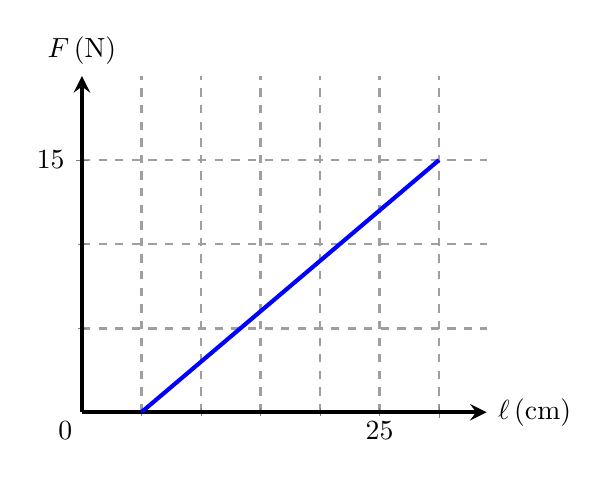
\begin{tikzpicture}  
			\begin{axis}[  ultra thick, scale=0.75,
				xmin=0,  
				xmax=34,  
				xtick={0,30},
				ytick={0,15},
				minor x tick num=5,
				minor y tick num=2,
				xticklabels=\empty,
				ymin=0,  
				ymax=20, 
				samples=300,
				axis lines=center, 
				grid style={step=1, line width=1pt, gray!75!white, dashed},
				grid=both, %giới hạn ô lưới
				major grid style={line width=1pt, gray!75!white, dashed},
				xlabel=$\xsi{\ell}{\left(\si{\centi\meter}\right)}$, 		ylabel=$\xsi{F}{\left(\si{\newton}\right)}$,
				every axis y label/.style={at=(current axis.above origin),anchor=south},  
				every axis x label/.style={at=(current axis.right of origin),anchor=west},  ]
				\addplot [line width=1.5pt, blue, smooth, domain=5:30] {0.6*(x-5)};  
				\coordinate (O) at (axis cs: 0,0);
				\coordinate (x) at (axis cs: 25,0);
			\end{axis}  
			\node[below left] at (O) {0};
			\node[below] at (x) {$25$};
		\end{tikzpicture}
	\end{center}
	\choiceTF[t]
	{\True Chiều dài tự nhiên của lò xo là $\SI{5}{\centi\meter}$}
	{\True Khi lò xo dài $\SI{30}{\centi\meter}$ thì lực đàn hồi có giá trị bằng $\SI{15}{\newton}$}
	{Lò xo này đang bị nén}
	{\True Độ cứng của lò xo $k=\SI{60}{\newton/\meter}$}
	\loigiai{}
\end{ex}
% ===================================================================
\begin{ex}\mkstar{3}
Treo vật có khối lượng $\SI{500}{\gram}$ vào một lò xo thì làm nó dãn ra $\SI{5}{\centi\meter}$. Cho $g=\SI{10}{\meter/\second^2}$.
	\choiceTF[t]
	{\True Trọng lực của vật có tác dụng làm cho lò xo dãn ra}
	{Trong giới hạn đàn hồi, nếu treo vật có kích thước càng lớn thì độ dãn của lò xo càng lớn}
	{\True Độ cứng của lò xo là $\SI{100}{\newton/\meter}$}
	{Treo thêm vào lò xo vật $m'=\SI{1}{\kilogram}$ thì lò xo dãn $\SI{10}{\centi\meter}$}
	\loigiai{}
\end{ex}
\Closesolutionfile{ans}
\section{Tự luận}
\setcounter{ex}{0}
\Opensolutionfile{ans}[ans/VN10-Y24-PH-SYL-033P-TL]
% ======================================================================
\begin{ex}\mkstar{2}
	Treo một vật có trọng lượng $\SI{2.0}{N}$ vào một cái lò xo, lò xo dãn ra $\SI{10}{mm}$. Treo một vật khác có trọng lượng chưa biết vào lò xo, nó dãn ra $\SI{80}{mm}$.
	\begin{enumerate}[label=\alph*)]
		\item Tính độ cứng của lò xo.
		\item Tính trọng lượng chưa biết.
	\end{enumerate}
	\loigiai{\begin{enumerate}[label=\alph*)]
			\item Khi treo vật có trọng lượng $P_1=\SI{2.0}{N}$ thì $\Delta l_1 = \SI{10e-3}{m}$. Khi đó trọng lực và lưc đàn hồi cân bằng nên
			$$F_\text{đh 1} = P_1 = k |\Delta l_1| \Rightarrow k = \SI{200}{N/m}$$
			
			\item Tính trọng lượng chưa biết.
			
			$$P_2 = F_\text{đh 2} =k |\Delta l_2| = \SI{16}{N} $$
	\end{enumerate}}
\end{ex}
% ======================================================================
\begin{ex}\mkstar{2}
	Một học sinh thực hiện thí nghiệm đo độ cứng của một lò xo và thu được kết quả như hình. Độ cứng của lò xo này có giá trị bằng bao nhiêu?
	\begin{center}
		\includegraphics[width=0.4\linewidth]{../figs/VN10-2023-PH-TP033-4}
		\captionof{figure}{Kết quả thí nghiệm đo độ cứng lò xo.}
	\end{center}
	\loigiai{Ta có:
		$$F_\text{đh}=P$$
		$$\Leftrightarrow k\Delta\ell=P$$
		$$\Rightarrow k=\dfrac{P}{\Delta\ell}=\dfrac{\SI{1}{\newton}}{\SI{0.05}{\meter}}=\SI{20}{\newton/\meter}.$$}
\end{ex}
% ======================================================================
\begin{ex}\mkstar{3}
	Một lò xo có độ cứng $\SI{100}{N/m}$ được treo thẳng đứng vào một điểm cố định, đầu dưới gắn với vật khối lượng $\SI{1}{kg}$. Vật được đặt trên giá đỡ D. Ban đầu giá đỡ D đứng yên và lò xo dãn $\SI{1}{cm}$. Cho D chuyển động nhanh dần đều hướng xuống với gia tốc $\SI{1}{m/s^2}$. Bỏ qua mọi ma sát và lực cản. Lấy $g=\SI{10}{m/s^2}$. Tính quãng đường mà giá đỡ đi được từ lúc bắt đầu chuyển động đến khi vật rời khỏi giá đỡ và tốc độ của vật khi đó.
	\loigiai{Độ biến dạng của lò xo khi treo vật:
		$$\Delta \ell = \SI{10}{cm}$$
		Áp dụng định luật II Newton cho vật nặng trong quá trình lò xo dãn:
		$$\vec P+\vec N+\vec F_\text{đh}=m\vec a$$
		Chiếu phương trình định luật II Newton lên chiều trọng lực:
		$$P-N-F_\text{đh}=ma$$
		$$\Rightarrow N=P-F_\text{đh}-ma$$
		Khi vật nặng rời khỏi giá đỡ $N=0$:
		$$F_\text{đh}=m\left(g-a\right)\Rightarrow \Delta\ell=\dfrac{m\left(g-a\right)}{k}=\SI{0.09}{\meter}=\SI{9}{\centi\meter}$$
		Mà khi đặt trên D thì lò xo bị dãn $\SI{1}{cm}$, nên lò xo cần dãn thêm $\SI{8}{cm}$ nữa thì vật sẽ rời khỏi D.\\
		Vậy quãng đường mà D đi xuống thêm được là $s=\SI{8}{cm}$.\\
		Áp dụng công thức:
		$$v^2 -0 = 2aS \Rightarrow v = \SI{40}{cm/s}$$}
\end{ex}
% ======================================================================
\begin{ex}\mkstar{3}
\immini{	Một lò xo treo thẳng đứng gồm lò xo nhẹ và vật nhỏ A có khối lượng $m_{\mathrm{A}}$. Lần lượt treo thêm các quả cân vào A thì độ dãn của lò xo tương ứng là $\Delta \ell$. Hình bên biểu diễn sự phụ thuộc của $\Delta\ell$ theo tổng khối lượng $\Delta m$ của các quả cân treo vào A. Tính giá trị của $m_{\mathrm{A}}$.}
{
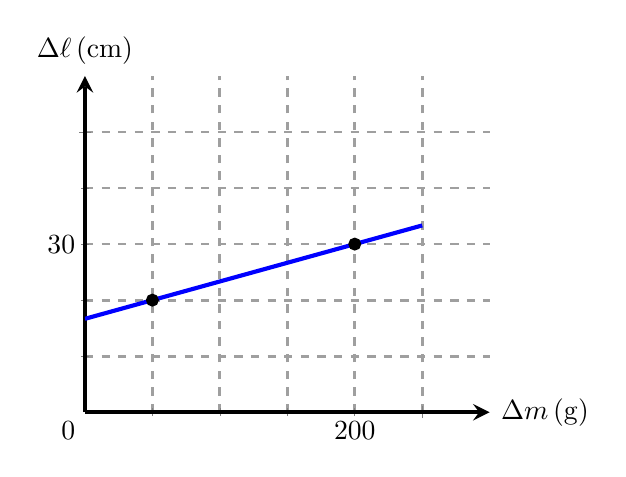
\begin{tikzpicture}  
	\begin{axis}[  ultra thick, scale=0.75,
		xmin=0,  
		xmax=300,  
		xtick={0,250},
		ytick={0,50},
		minor x tick num=4,
		minor y tick num=4,
		xticklabels=\empty,
		yticklabels=\empty,
		ymin=0,  
		ymax=60, 
		samples=300,
		axis lines=center, 
		grid style={step=1, line width=1pt, gray!75!white, dashed},
		grid=both, %giới hạn ô lưới
		major grid style={line width=1pt, gray!75!white, dashed},
		xlabel=$\xsi{\Delta m}{\left(\si{\gram}\right)}$, 		ylabel=$\xsi{\Delta \ell}{\left(\si{\centi\meter}\right)}$,
		every axis y label/.style={at=(current axis.above origin),anchor=south},  
		every axis x label/.style={at=(current axis.right of origin),anchor=west},  ]
		\addplot [line width=1.5pt, blue, smooth, domain=0:250] {20+(x-50)/15};  
		\coordinate (O) at (axis cs: 0,0);
		\coordinate (x) at (axis cs: 200,0);
		\coordinate (y) at (axis cs: 0,30);
		\filldraw[black] (axis cs: 50,20) circle(1.5pt);
		\filldraw[black] (axis cs: 200,30) circle(1.5pt);
	\end{axis}  
	\node[below left] at (O) {0};
	\node[below] at (x) {$200$};
	\node[left] at (y) {$30$};
\end{tikzpicture}
}
	\loigiai{
	Ta cosL $k\Delta\ell=\left(m_{\mathrm{A}}+\Delta m\right)g$.\\
	Vậy: $\dfrac{\Delta \ell_1}{\Delta \ell_2}=\dfrac{m_{\mathrm{A}}+\Delta m_1}{m_{\mathrm{A}}+\Delta m_2}$.\\
	Với $\Delta \ell_1=\SI{20}{\centi\meter}$, $\Delta m_1=\SI{50}{\gram}$, $\Delta\ell_2=\SI{30}{\centi\meter}$, $\Delta m_2=\SI{200}{\gram}$.\\
	Tính được $m_{\mathrm{A}}=\SI{250}{\gram}$.
	}
\end{ex}
% ======================================================================
\begin{ex}\mkstar{4}
	Một lò xo khối lượng không đáng kể, độ cứng $\SI{100}{N/m}$ và có chiều dài tự nhiên $\SI{40}{cm}$. Giữ đầu trên của lò xo cố định và buộc vào đầu dưới của lò xo một vật nặng khối lượng $\SI{500}{g}$, sau đó lại buộc thêm vào điểm chính giữa của lò xo đã bị dãn thêm một vật thứ hai khối lượng $\SI{500}{g}$. Lấy $g=\SI{10}{m/s^2}$. Tính chiều dài của lò xo khi đó.
	\loigiai{Chiều dài của lò xo khi treo vật thứ nhất:
		$$l_1 = l_0 + \Delta l_1 = l_0 + \dfrac{m_1g}{k} = \SI{45}{cm}$$
		Treo thêm vật thứ hai vào điểm chính giữa của lò xo đang dãn ($l_2 = \dfrac{l_1}{2} = \SI{22.5}{cm}$) thì tương ứng với cắt lò xo ra còn một nửa 
		$$k_1l_1= k_2 l_2 \Rightarrow k_2 = \dfrac{k_1l_1}{l_2} = \SI{200}{N/m}$$
		Độ biến dạng thêm của lò xo khi treo vật thứ hai:
		$$\Delta l_2 = \SI{2.5}{cm}$$
		Vậy với chiều dài khi theo vật thứ nhất là $\SI{45}{cm}$ mà còn biến dạng thêm một đoạn $\SI{2.5}{cm}$ thì chiều dài lò xo lúc này là $\SI{47.5}{cm}$.}
\end{ex}
\Closesolutionfile{ans}
				\stopMyChapterToc
		\stopPartToc
	\chapter*{Ôn tập chương \thepart}
	\addcontentsline{toc}{mychapter}{\bfseries Ôn tập chương \thepart}
	\let\lesson\undefined
\newcommand{\lesson}{\phantomlesson{Ôn tập chương 9}}
\setcounter{section}{2}
\setcounter{ex}{0}
\Opensolutionfile{ans}[ans/VN10-2023-PH-TP0009-TN]
% ===================================================================
\begin{ex}\mkstar{1}
Lực đàn hồi xuất hiện tỉ lệ với độ biến dạng khi 	
	\choice
	{một vật bị biến dạng dẻo}
	{\True một vật biến dạng đàn hồi}
	{một vật bị biến dạng}
	{ta ấn ngón tay vào một viên đất nặn}
	\loigiai{Lực đàn hồi xuất hiện tỉ lệ với độ biến dạng khi một vật biến dạng đàn hồi.}
\end{ex}
% ===================================================================
\begin{ex}\mkstar{1}
	Kết luận nào sau đây \textbf{không} đúng đối với lực đàn hồi?
	\choice
	{Xuất hiện khi vật bị biến dạng}
	{\True Luôn là lực kéo}
	{Tỉ lệ với độ biến dạng}
	{Ngược hướng với lực làm nó bị biến dạng}
	\loigiai{	Lực đàn hồi có khi là lực kéo, có khi là lực nén.}
\end{ex}
% ===================================================================
\begin{ex}\mkstar{1}
Điều nào sau đây là \textbf{sai} khi nói về phương và độ lớn của lực đàn hồi?	
	\choice
	{Với cùng độ biến dạng như nhau, độ lớn của lực đàn hồi phụ thuộc vào kích thước và bản chất của vật đàn hồi}
	{Với các mặt tiếp xúc bị biến dạng, lực đàn hồi vuông góc với các mặt tiếp xúc}
	{Với các vật như lò xo, dây cao su, thanh dài, lực đàn hồi hướng dọc theo trục của vật}
	{\True Lực đàn hồi có độ lớn tỉ lệ nghịch với độ biến dạng của vật biến dạng}
	\loigiai{Lực đàn hồi tỉ lệ thuận với độ biến dạng của vật biến dạng.}
\end{ex}
% ===================================================================
\begin{ex}\mkstar{1}
	Khẳng định nào sau đây là đúng khi ta nói về lực đàn hồi của lò xo và lực căng của dây?
	\choice
	{\True Đó là những lực chống lại sự biến dạng đàn hồi của lò xo và sự căng của dây}
	{Đó là những lực gây ra sự biến dạng đàn hồi của lò xo và sự căng của dây}
	{Chúng đều là những lực kéo}
	{Chúng đều là những lực đẩy}
	\loigiai{Lực đàn hồi của lò xo và lực căng của dây: đó là những lực chống lại sự biến dạng đàn hồi của lò xo và sự căng của dây.}
\end{ex}
% ===================================================================
\begin{ex}\mkstar{1}
	Một vật tác dụng một lực vào một lò xo có đầu cố định và làm lò xo biến dạng. Điều nào dưới đây là \textbf{không đúng}?
	\choice
	{Độ đàn hồi của lò xo có độ lớn bằng lực tác dụng và chống lại sự biến dạng của lò xo}
	{Lực đàn hồi cùng phương và ngược chiều với lực tác dụng}
	{\True Lực đàn hồi lớn hơn lực tác dụng và chống lại lực tác dụng}
	{Khi vật ngừng tác dụng lên lò xo thì lực đàn hồi của lò xo cũng mất đi}
	\loigiai{}
\end{ex}
% ===================================================================
\begin{ex}\mkstar{1}
Chọn phát biểu \textbf{sai} về lực đàn hồi của lò xo.	
	\choice
	{Lực đàn hồi của lò xo có xu hướng chống lại nguyên nhân gây ra biến dạng}
	{Lực đàn hồi của lò xo dài có phương là trục lò xo, chiều ngược với chiều biến dạng của lò xo}
	{Lực đàn hồi của lò xo có độ lớn tuân theo định luật Hooke}
	{\True Lực đàn hồi của lò xo chỉ xuất hiện ở đầu lò xo đặt ngoại lực gây biến dạng}
	\loigiai{Lực đàn hồi xuất hiện ở hai đầu của lò xo và tác dụng vào các vật tiếp xúc (hay gắn) với lò xo làm nó biến dạng.}
\end{ex}
% ===================================================================
\begin{ex}\mkstar{1}
Lực đàn hồi của lò xo có tác dụng làm cho lò xo	
	\choice
	{chuyển động}
	{thu gia tốc}
	{\True có xu hướng lấy lại hình dạng và kích thước ban đầu}
	{vừa biến dạng vừa thu gia tốc}
	\loigiai{}
\end{ex}
% ===================================================================
\begin{ex}\mkstar{2}
	Một lò xo có chiều dài tự nhiên là $\SI{20}{cm}$. Khi lò xo có chiều dài $\SI{24}{cm}$ thì lực đàn hồi của nó bằng $\SI{5}{N}$. Hỏi khi lực đàn hồi của lò xo bằng $\SI{10}{N}$ thì chiều dài của nó bằng bao nhiêu?
	\choice
	{$\SI{22}{cm}$}
	{\True $\SI{28}{cm}$}
	{$\SI{40}{cm}$}
	{$\SI{48}{cm}$}
	\loigiai{Ta có:
		$$F = k \Delta l.$$
		Vậy: 
		$$F_1 = k \Delta l_1; F_2 = k \Delta l_2.$$
		Lập tỉ số:
		$$\dfrac{F_1}{F_2} = \dfrac{\Delta l_1}{\Delta l_2} \Rightarrow \Delta l_2 = \SI{0,08}{m} = \SI{8}{cm}.$$
		Chiều dài của lò xo là
		$$l' = l_0 + \Delta l_2 = \SI{28}{cm}.$$}
\end{ex}
% ===================================================================
\begin{ex}\mkstar{2}
	Một lò xo có chiều dài tự nhiên bằng $\SI{22}{cm}$. Lò xo được treo thẳng đứng, một đầu giữ cố định, còn đầu kia gắn một vật nặng. Khi ấy lò xo dài $\SI{27}{cm}$, cho biết độ cứng lò xo là $\SI{100}{N/m}$. Độ lớn lực đàn hồi bằng 	
	\choice
	{$\SI{500}{N}$}
	{\True $\SI{5}{N}$}
	{$\SI{20}{N}$}
	{$\SI{50}{N}$}
	\loigiai{Độ biến dạng của lò xo:
		$$\Delta l = l-l_0 = \SI{5}{cm} = \SI{0,05}{m}.$$
		Độ lớn của lực đàn hồi:
		$$F_\text{đh} = k\Delta l = \SI{5}{N}.$$}
\end{ex}
% ===================================================================
\begin{ex}\mkstar{2}
	Phải treo một vật có khối lượng bằng bao nhiêu vào lò xo có độ cứng $\SI{100}{N/m}$ để lò xo dãn ra được $\SI{10}{cm}$? Lấy $g = \SI{10}{m/s}^2$.
	\choice
	{\True $\SI{1}{kg}$}
	{$\SI{10}{kg}$}
	{$\SI{100}{kg}$}
	{$\SI{1000}{kg}$}
	\loigiai{Ta có: 
		$$F_\text{đh} = k\Delta l = \SI{10}{N}.$$
		Mà $F_\text{đh} = P.$\\
		Suy ra:
		$$m = \dfrac{P}{g} = \SI{1}{kg}.$$}
\end{ex}
	
% ===================================================================
\begin{ex}\mkstar{2}
Dùng một lò xo để treo một vật có khối lượng $\SI{300}{g}$ thì thấy lò xo dãn một đoạn $\SI{2}{cm}$. Nếu treo thêm một vật có khối lượng $\SI{150}{g}$ thì độ dãn của lò xo là	
	\choice
	{$\SI{1}{cm}$}
	{$\SI{2}{cm}$}
	{\True $\SI{3}{cm}$}
	{$\SI{4}{cm}$}
	\loigiai{Khi treo vật khối lượng $\SI{300}{g}$:
		$$m_1g = k\Delta l_1 \Rightarrow k = \dfrac{m_1 g}{\Delta l_1}.$$
		Khi treo thêm một vật ta có:
		$$(m_1+m_2)g = k\Delta l_2 \Rightarrow \Delta l_2 = \dfrac{(m_1+m_2)g}{k} = \SI{0,03}{m} = \SI{3}{cm}.$$}
\end{ex}
% ===================================================================
\begin{ex}\mkstar{2}
	Một lò xo có chiều dài tự nhiên bằng $\SI{20}{cm}$. Khi bị kéo lò xo dài $\SI{24}{cm}$ và lực đàn hồi của nó bằng $\SI{5}{N}$. Hỏi khi lực đàn hồi của lò xo bằng $\SI{15}{N}$ thì chiều dài của nó bằng bao nhiêu?
	\choice
	{$\SI{28}{cm}$}
	{\True $\SI{32}{cm}$}
	{$\SI{45}{cm}$}
	{$\SI{20}{cm}$}
	\loigiai{	Ta có:	
		$$F = k \Delta l.$$	
		Vậy: 
		$$F_1 = k \Delta l_1; F_2 = k \Delta l_2.$$	
		Lập tỉ số:	
		$$\dfrac{F_1}{F_2} = \dfrac{\Delta l_1}{\Delta l_2} \Rightarrow \Delta l_2 = \SI{0,12}{m} = \SI{12}{cm}.$$	
		Chiều dài của lò xo là	
		$$l' = l_0 + \Delta l_2 = \SI{32}{cm}.$$}
\end{ex}

% ===================================================================
\begin{ex}\mkstar{3}
Một lò xo có chiều dài tự nhiên $\ell_0=\SI{27}{\centi\meter}$, được treo thẳng đứng. Khi treo vào một vật có trọng lượng $P_1=\SI{5}{\newton}$ thì lò xo dài $\ell_1=\SI{44}{\centi\meter}$. Khi treo vật khác có trọng lượng $P_2$ chưa biết, lò xo dài $\ell_2=\SI{35}{\centi\meter}$. Độ cứng của lò xo và trọng lượng $P_2$ là	
	\choice
	{$k=\SI{25.3}{\newton/\meter}$, $P_2=\SI{2.35}{\newton}$}
	{\True $k=\SI{29.4}{\newton/\meter}$, $P_2=\SI{2.35}{\newton}$}
	{$k=\SI{25.3}{\newton/\meter}$, $P_2=\SI{3.5}{\newton}$}
	{$k=\SI{29.4}{\newton/\meter}$, $P_2=\SI{3.5}{\newton}$}
	\loigiai{Độ cứng lò xo:
		$$k=\dfrac{P_1}{\ell_1-\ell_0}=\dfrac{\left(\SI{5}{\newton}\right)}{\SI{0.44}{\meter}-\SI{0.27}{\meter}}\approx\SI{29.4}{\newton/\meter}$$
		Trọng lượng $P_2$:
		$$P_2=k\left|\Delta\ell_2\right|=\left(\SI{29.4}{\newton/\meter}\right)\cdot\left|\SI{0.35}{\meter}-\SI{0.27}{\meter}\right|\approx\SI{2.35}{\newton}.$$}
\end{ex}
% ===================================================================
\begin{ex}\mkstar{3}
	Một lò xo có độ cứng $k$, chiều dài tự nhiên $\ell_0$ được treo thẳng đứng, đầu trên cố định. Khi người ta treo quả cân có khối lượng $\SI{200}{\gram}$ vào đầu dưới của lò xo, lò xo có độ dài $\SI{32}{\centi\meter}$. Nếu treo thêm quả cân có khối lượng $\SI{500}{\gram}$ vào đầu dưới của lò xo thì lò xo có chiều dài $\SI{37}{\centi\meter}$. Lấy $g=\SI{10}{\meter/\second^2}$. Độ dài tự nhiên và độ cứng của lò xo là
	\choice
	{$\ell_0=\SI{30}{\centi\meter}$, $k=\SI{1000}{\newton/\meter}$}
	{$\ell_0=\SI{32}{\centi\meter}$, $k=\SI{300}{\newton/\meter}$}
	{$\ell_0=\SI{32}{\centi\meter}$, $k=\SI{2300}{\newton/\meter}$}
	{\True $\ell_0=\SI{30}{\centi\meter}$, $k=\SI{100}{\newton/\meter}$}
	\loigiai{Độ cứng của lò xo:
		$$k=\dfrac{m_2g}{\ell_2-\ell_1}=\dfrac{\left(\SI{0.5}{\kilogram}\right)\cdot\left(\SI{10}{\meter/\second^2}\right)}{\SI{0.37}{\meter}-\SI{0.32}{\meter}}=\SI{100}{\newton/\meter}$$
		Độ biến dạng của lò xo khi treo vật khối lượng $m_1=\SI{200}{\gram}$:
		$$\Delta\ell_1=\dfrac{m_1g}{k}=\SI{0.02}{\meter}=\SI{2}{\centi\meter}$$
		Độ dài tự nhiên của lò xo:
		$$\ell_0=\ell_1-\Delta\ell_1=\SI{30}{\centi\meter}.$$}
\end{ex}
% ===================================================================
\begin{ex}\mkstar{3}
Người ta treo một đầu lò xo vào một điểm cố định, đầu dưới của lò xo là những chùm quả nặng, mỗi quả đều có khối lượng $m$. Khi chùm quả nặng có 2 quả, chiều dài lò xo là $\SI{15}{\centi\meter}$. Khi chùm quả nặng có 4 quả, chiều dài lò xo là $\SI{17}{\centi\meter}$. Cho $g=\SI{10}{\meter/\second^2}$. Số quả nặng cần treo để lò xo dài $\SI{21}{\centi\meter}$ là	
	\choice
	{\True 8 quả}
	{10 quả}
	{6 quả}
	{9 quả}
	\loigiai{Độ biến dạng của lò xo khi treo quả nặng:
		\begin{eqnarray*}
			&&\Delta\ell=\dfrac{mg}{k}\\
			&\Rightarrow& \dfrac{\ell_2-\ell_1}{\ell_3-\ell_1}=\dfrac{\left(m_2-m_1\right)g}{\left(m_3-m_1\right)g}\\
			&\Leftrightarrow& \dfrac{4m-2m}{N\cdot m-2m}=\dfrac{\SI{17}{\centi\meter}-\SI{15}{\centi\meter}}{\SI{21}{\centi\meter}-\SI{15}{\centi\meter}}\\
			&\Rightarrow& N=8.
	\end{eqnarray*}}
\end{ex}
% ===================================================================
\begin{ex}\mkstar{3}
	\immini{Một vật có khối lượng $M$ được gắn vào một dầu của lò xo có độ cứng $k$ được đặt trên mặt phẳng nghiêng góc $\theta$ so với phương ngang, bỏ qua ma sát giữa vật và mặt nghiêng, vật ở trạng thái đứng yên. Độ dãn của lò xo là
	\choice
	{$x=\dfrac{2Mg\sin\theta}{k}$}
	{\True $x=\dfrac{Mg\sin\theta}{k}$}
	{$x=\dfrac{Mg}{k}$}
	{$x=\sqrt{2Mg}$}
	}
	{\includegraphics[scale=0.7]{../figs/VN10-2023-PH-TP0009-1}}
	\loigiai{Vật nhỏ cân bằng:
		\begin{equation}
			\label{eq:0009-1}
			\vec P+\vec N+\vec F_\text{đh}=\vec 0
		\end{equation}
		Chiếu phương trình (\ref{eq:0009-1}) lên phương song song măt nghiêng:
		\begin{eqnarray*}
			&&P\sin\theta=F_\text{đh}\\
			&\Leftrightarrow& mg\sin\theta=kx\\
			&\Rightarrow& x=\dfrac{Mg\sin\theta}{k}.
	\end{eqnarray*}}
\end{ex}
% ===================================================================
\begin{ex}\mkstar{3}
\immini{Hai lò xo A và B được bố trí như hình vẽ. Độ cứng của lò xo A là $k_A=\SI{100}{\newton/\meter}$. Khi kéo đầu tự do của lò xo B ra, lò xo A dãn $\SI{5}{\centi\meter}$, lò xo B dãn $\SI{1}{\centi\meter}$. Độ cứng của lò xo B là
\choice
{$\SI{100}{\newton\meter}$}
{$\SI{25}{\newton/\meter}$}
{$\SI{350}{\newton/\meter}$}
{\True $\SI{500}{\newton/\meter}$}
}	
{\includegraphics[scale=0.7]{../figs/VN10-2023-PH-TP0009-2}}
	\loigiai{Vì hai lò xo được ghép nối tiếp, lực đàn hồi trên hai lò xo có độ lớn như nhau:
		\begin{eqnarray*}
			&&F_\text{đh A}=F_\text{đh B}\\
			&\Leftrightarrow& \dfrac{k_B}{k_A}=\dfrac{\Delta\ell_A}{\Delta\ell_B}=5\\
			&\Rightarrow& k_B=5k_A=\SI{500}{\newton/\meter}.
	\end{eqnarray*}}
\end{ex}
% ===================================================================
\begin{ex}\mkstar{3}
	\immini{Hai lò xo giống nhau có cùng độ cứng $\SI{100}{\newton/\meter}$ được bố trí như hình vẽ. Vật $m$ có khối lượng $\SI{200}{\gram}$. Khi vật nặng cân bằng, độ dãn của mỗi lò xo là
	\choice
	{\True $\SI{1}{\centi\meter}$}
	{$\SI{2}{\centi\meter}$}
	{$\SI{1.5}{\centi\meter}$}
	{$\SI{3}{\centi\meter}$}
	}
	{\includegraphics[scale=0.5]{../figs/VN10-2023-PH-TP0009-4}}
	\loigiai{Vật nặng cân bằng:
		$$F_\text{đh 1}+F_\text{đh 2}=mg$$
		$$\Leftrightarrow \Delta\ell=\dfrac{mg}{2k}=\SI{0.01}{\meter}=\SI{1}{\centi\meter}.$$}
\end{ex}
% ===================================================================
\begin{ex}\mkstar{3}
	\immini{Hình bên là đồ thị gồm hai đường thẳng xiên góc đi qua gốc toạ độ $O$, mô tả sự thay đổi giá trị của lực đàn hồi theo các độ dãn khác nhau của lò xo X và lò xo Y. Chọn kết luận đúng về độ cứng của hai lò xo.
	\choice
	{$k_X<k_Y$}
	{$k_X\le k_Y$}
	{$k_X=k_Y$}
	{\True $k_X>k_Y$}
	}
	{\includegraphics[scale=0.6]{../figs/VN10-2023-PH-TP0009-3}}
	\loigiai{Với cùng độ lớn lực đàn hồi, lò xo Y dãn nhiều hơn lò xo X, do đó:
		$$k_X>k_Y.$$}
\end{ex}
\Closesolutionfile{ans}
\end{document}